% =============================================================================
%  Kapustin & Witten, "Electric-Magnetic Duality And The Geometric Langlands
%  Program" —— 中文学术译注本
%
%  原文：A. Kapustin & E. Witten, arXiv:hep-th/0604151v3 (231 pp.)
%  编译：xelatex main.tex 三遍（或 python tools/build.py）
%
%  体例：
%    * 公式编号锁定原文编号（脚手架已写 \setcounter{equation}{N}），可与原文逐式对照；
%    * 36 个片段 zh/NN-sXX.tex 依次 \input；
%    * 「本节重点」（蓝框）与「译注」（橙框）为译者所加，非原文内容；
%    * 译注可一键关闭：\showyizhutrue → \showyizhufalse。
% =============================================================================
\documentclass[11pt,a4paper]{article}

%% 导言区（由 tools/split_preamble.py 从 main.tex 抽出，请直接改这里）
\usepackage[UTF8, fontset=windows, heading=true]{ctex}
\usepackage{amsmath}
\usepackage{amssymb}
\usepackage{bm}
\usepackage[a4paper,left=2.5cm,right=2.5cm,top=2.6cm,bottom=2.6cm]{geometry}
\usepackage{graphicx}
\usepackage{xcolor}
\usepackage[most]{tcolorbox}
\usepackage{enumitem}
\usepackage{booktabs}
\usepackage{array}
\usepackage{longtable}
\usepackage{multirow}
\usepackage[font=small,labelfont=bf,labelsep=quad]{caption}
\usepackage[sort,compress]{cite}
\usepackage[colorlinks=true,
            linkcolor=blue!45!black,
            citecolor=blue!45!black,
            urlcolor=blue!45!black]{hyperref}

\numberwithin{equation}{section}
\setlength{\emergencystretch}{3em}
\allowdisplaybreaks[3]
\linespread{1.12}
\renewcommand{\figurename}{图}
\renewcommand{\tablename}{表}
\ctexset{
  section/name    = {},
  section/number  = \arabic{section},
  subsection/name = {},
  subsubsection/name = {},
}

% ---------- 「本节重点」（译者所加） ----------
\newtcolorbox{keytakeaways}[1][本节重点]{
  enhanced,
  colback  = blue!3!white,
  colframe = blue!35!black,
  boxrule  = 0.4pt,
  arc      = 2pt,
  left     = 7pt, right = 7pt, top = 5pt, bottom = 5pt,
  title    = {#1\,{\normalfont\scriptsize（译者所加）}},
  fonttitle= \bfseries\small,
  before skip = 10pt, after skip = 10pt,
}

% ---------- 译注（译者所加，成品中可见；可一键关闭） ----------
\newif\ifshowyizhu
\showyizhutrue
\newcounter{yizhu}
\makeatletter
\newenvironment{yizhu}[1][]{%
  \ifshowyizhu
    \refstepcounter{yizhu}%
    \par\addvspace{5pt}\noindent
    \begin{tcolorbox}[enhanced, breakable,
      colback  = orange!4!white,
      colframe = orange!55!black,
      boxrule  = 0.3pt,
      arc      = 1.5pt,
      left     = 6pt, right = 6pt, top = 4pt, bottom = 4pt,
      title    = {\small\bfseries 译注~\theyizhu
                  \if\relax\detokenize{#1}\relax\else\ ——#1\fi}]%
    \small
  \else
    \setbox\z@\vbox\bgroup\small
  \fi
}{%
  \ifshowyizhu
    \end{tcolorbox}%
  \else
    \egroup
  \fi
}
\makeatother


% ---------- 上下文自适应字体宏（harvmac 的 {\it x} {\bf x} {\rm x} 在文本/数学两处都出现） ----------
\newcommand{\myit}[1]{\ifmmode\mathit{#1}\else\textit{#1}\fi}
\newcommand{\mybf}[1]{\ifmmode\mathbf{#1}\else\textbf{#1}\fi}
\newcommand{\myrm}[1]{\ifmmode\mathrm{#1}\else\textrm{#1}\fi}

% ---------- 原文 harvmac 记号宏（自动移植） ----------
%% KW06 记号宏：由 tools/harvmac2tex.py 自动抽取（勿手改；新增请写 macros-extra.tex）
\def\Bbb#1{\mathbb{#1}}
\def\frak#1{\mathfrak{#1}}
\def\cal#1{\mathcal{#1}}
\def\bf#1{\mathbf{#1}}
\def\it#1{\textit{#1}}
\def\rm#1{\mathrm{#1}}
\def\BG{{\overline \Gamma}}
\def\CC{{\Bbb{C}}}
\def\CM{{\EUM}}
\def\CZ{{\cal Z}}
\def\EUA{\eusm A}
\def\EUB{\eusm B}
\def\EUBB{\cmmib B}
\def\EUC{\eusm C}
\def\EUD{\eusm D}
\def\EUE{\eusm E}
\def\EUF{\eusm F}
\def\EUG{\eusm G}
\def\EUH{\eusm H}
\def\EUI{\eusm I}
\def\EUJ{\eusm J}
\def\EUK{\eusm K}
\def\EUL{\eusm L}
\def\EUM{\eusm M}
\def\EUN{\eusm N}
\def\EUO{\eusm O}
\def\EUP{\eusm P}
\def\EUQ{\eusm Q}
\def\EUR{\eusm R}
\def\EUS{\eusm S}
\def\EUT{\eusm T}
\def\EUU{\eusm U}
\def\EUV{\eusm V}
\def\EUW{\eusm W}
\def\EUWW{\eurm W}
\def\EUX{\eusm X}
\def\EUY{\eusm Y}
\def\EUZ{\eusm Z}
\def\End{{\rm End}}
\def\G{{\Gamma}}
\def\Gad{{G_{\rm ad}}}
\def\HG{{\widehat \Gamma}}
\def\Im{{\rm Im ~}}
\def\LG{{^L\negthinspace G}}
\def\M{{\EUM}}
\def\MH{{{\EUM}_H}}
\def\MHAD{\MH(G_{\rm ad})}
\def\N{{\EUN}}
\def\PP{{\Bbb{P}}}
\def\R{{\bf R}}
\def\RR{{\Bbb{R}}}
\def\Re{{\rm Re ~}}
\def\S{{\bf S}}
\def\T{{\bf T}}
\def\Tr{{\rm Tr}}
\def\Z{{\bf Z}}
\def\ZZ{\hbox{\zfont Z\kern-.4emZ}}
\def\ad{\rm {ad}}
\def\bar{\overline}
\def\bigone{\hbox{1\kern -.23em {\rm l}}}
\def\botampo{fig.~12}
\def\bpartial{{\bar\partial}}
\def\bsigma{{\bar\sigma}}
\def\bt{{\bar t}}
\def\by{{\bar y}}
\def\bz{{\bar z}}
\def\cA{{\cal A}}
\def\cD{{\cal D}}
\def\cF{{\cal F}}
\def\cI{{\cal I}}
\def\cJ{{\cal J}}
\def\cK{{\cal K}}
\def\cL{{\cal L}}
\def\cM{{\EUM}}
\def\cN{{\EUN}}
\def\cO{{\cal O}}
\def\cQ{{\cal Q}}
\def\dunamp{fig.~6}
\def\eps{\epsilon}
\def\figin{\epsfcheck\figin}
\def\figins{\epsfcheck\figins}
\def\g{{\frak g}}
\def\gog{{\frak g}}
\def\half{{\litfont {1 \over 2}}}
\def\hat{\widehat}
\def\namp{fig.~4}
\def\neg{\negthinspace}
\def\notampo{fig.~14}
\def\ot{\otimes}
\def\otampo{fig.~13}
\def\pf{{\rm Pf ~}}
\def\quadramp{fig.~8}
\def\quintamp{fig.~9}
\def\ra{\rightarrow}
\def\rr{r}
\def\sdtimes{\mathbin{\hbox{\hskip2pt\vrule
height 4.1pt depth -.3pt width .25pt\hskip-2pt$\times$}}}
\def\tI{{\tilde I}}
\def\tg{{\frak t}}
\def\tilde{\widetilde}
\def\tonamp{fig.~5}
\def\tpsi{{\tilde\psi}}
\def\trampo{fig.~3}
\def\trinamp{fig.~7}
\def\utampo{fig.~15}
\def\xdtampo{fig.~18}
\def\xitampo{fig.~19}
\def\xtampo{fig.~17}
\def\xunko{fig.~2}
\def\xutampo{fig.~16}
\def\xytampo{fig.~20}
\def\zingop{fig.~10}
\def\zunko{fig.~1}

%% =============================================================================
%%  macros-extra.tex —— 转换器输出（macros.tex）之外的人工补丁
%%  每次重跑 tools/harvmac2tex.py 都不会覆盖本文件；preamble.tex 在 macros 之后 input 它。
%% =============================================================================

%% ---- 1. harvmac 用的 euler 字体在本机不存在，用 LaTeX 数学字母代替 ----
\def\eusm#1{{\cal #1}}
\def\eurm#1{{\rm #1}}
\def\cmmib#1{{\bf #1}}
\def\Tr{\operatorname{Tr}}
\def\tr{\operatorname{tr}}

%% ---- 2. 原文正文中段才定义、只被导言区抽取漏掉的记号 ----
\def\CMF{{\cmmib F}}
\def\CF{{\cal F}}
\def\VV{{\eurm V}}
\def\bone{{\bf 1}}
\def\btwo{{\bf 2}}
\def\b4{{\bf 4}}
\def\bb4{{\bf \bar 4}}

%% ---- 3. 源文件中从未定义（疑为旧版 harvmac 残留），按上下文补 ----
\def\lie{{\cal L}}
\def\CA{{\cal A}}
\def\CO{{\cal O}}

%% ---- 4. plain TeX 写法 / 字体切换宏的 shim ----
\def\half{\frac{1}{2}}
\def\litfont{}
\def\tenrm{}\def\sevenrm{}\def\fiverm{}
\def\tenbf{}\def\sevenbf{}\def\fivebf{}
\def\tenit{}\def\sevenit{}\def\teniit{}
\def\tensy{}\def\sevensy{}\def\fivesy{}
\makeatletter
\def\rightarrowfill{$\m@th\smash-\mkern-7mu\cleaders\hbox{$\mkern-2mu\smash-\mkern-2mu$}\hfill\mkern-7mu\mathord\rightarrow$}
\def\underarrow#1{\vbox{\ialign{##\crcr$\hfil\displaystyle{#1}\hfil$\crcr\noalign{\kern1pt\nointerlineskip}\rightarrowfill\crcr}}}
\makeatother


\hypersetup{
  pdftitle  = {电磁对偶与几何 Langlands 纲领（中译注本）},
  pdfauthor = {Anton Kapustin, Edward Witten（原著）；中文翻译与译注：DeepSeek Harness 智能体},
  pdfsubject = {Electric-Magnetic Duality; Geometric Langlands; 中文学术译注本},
  pdfkeywords = {电磁对偶, 几何Langlands纲领, 规范场论, 拓扑场论, Hitchin模空间, Hecke特征层},
}

\title{\bfseries 电磁对偶\\[2pt] \large 与几何 Langlands 纲领}
\author{Anton Kapustin \quad Edward Witten\\
        \small 加州理工学院物理系；普林斯顿高等研究院自然科学学院\\
        \small (California Institute of Technology; Institute for Advanced Study, Princeton)}
\date{arXiv:hep-th/0604151v3 \quad 2006 年 4 月（v3：2007 年 1 月）}



\begin{document}

% =============================================================================
%  front.tex —— 扉页、译本说明、体例说明
% =============================================================================
\begin{titlepage}
\centering
\vspace*{2.2cm}
{\LARGE\bfseries 电磁对偶}\\[10pt]
{\LARGE\bfseries 与几何 Langlands 纲领}\\[28pt]
{\large Electric-Magnetic Duality\\[4pt] And The Geometric Langlands Program}\\[34pt]
{\large Anton Kapustin \quad$\cdot$\quad Edward Witten}\\[26pt]
{\normalsize 中文学术译注本}\\[6pt]
{\small 译本附：思路导读、译注、译对报告、插件评估}\\[40pt]
{\small 底本：arXiv:hep-th/0604151v3 \quad 2006 年 4 月（v3：2007 年 1 月），231 页}\\[6pt]
{\small \today}
\vfill
\end{titlepage}

\thispagestyle{empty}
\section*{译本说明}
\addcontentsline{toc}{section}{译本说明}

\noindent\textbf{底本。}本译本的底本是 A.~Kapustin 与 E.~Witten 的
\emph{Electric-Magnetic Duality And The Geometric Langlands Program}
（arXiv:hep-th/0604151v3，231 页，12 节、362 个编号公式（由 348 处公式定义生成）、146 条参考文献）。译文直接从作者提交
arXiv 的 \LaTeX{} 源码（harvmac 格式）逐段生成，而不是从 PDF 文字层转写：公式、编号、
文献编号、图表都来自源码本身，因此可与原书逐式对照。

\medskip
\noindent\textbf{译文。}正文只放译文，不混入解释。译者所加的内容一律放进两类方框：
\begin{itemize}[leftmargin=1.6em,itemsep=2pt,topsep=2pt]
  \item \textbf{本节重点}（蓝框）：每节开头 3--5 条，交代该节要解决的问题、用到的工具、得到的结果；
  \item \textbf{译注}（橙框）：针对具体难点的补白，分「易错点」「含糊点拨」「物理图像」「原文疑误」四类。
\end{itemize}
译注可以整体关闭（\texttt{main.tex} 中 \verb|\showyizhutrue| 改为 \verb|\showyizhufalse|），
关闭后即为纯粹的译文。

\medskip
\noindent\textbf{编号。}编号公式与原文编号一一对应（如原文式 (3.41) 在本译本仍是式 (3.41)），
参考文献沿用原文的 [N] 编号。原文的图形按 \texttt{figures/} 下的图片重新排入，图号与原文一致。

\medskip
\noindent\textbf{原文疑误。}凡译者判断原文有笔误的地方，译文照原文保留，并紧接一条
「译注 [原文疑误]」说明理由与建议改法；不做静默修订。

\medskip
\noindent\textbf{致谢与声明。}原作者的版权、文字与观点归原作者所有；本译本仅供学习与研究使用，
译注部分的文责由译者承担。


\tableofcontents
\newpage

%% 自动生成：请勿手改（由 tools/build.py 生成）

%% ============================================================
%% 分片 01：原文第 1 节「Introduction」（原文 glshort.tex 起于第 313 行）
%% 由 tools/harvmac2tex.py 从 arXiv 源码（hep-th/0604151v3）自动生成。
%% 只译英文散文；公式、编号、\label、\cite 一律不改。
%% ============================================================

\section{引言}
\label{sec:intro}

\begin{keytakeaways}
\begin{itemize}[leftmargin=1.4em,itemsep=2pt,topsep=2pt]
\item \textbf{物理图像}：把 ${\EUN}=4$ 超对称杨-米尔斯理论放在 $\Sigma\times C$ 上、令 $\Sigma$ 的尺度趋于零，低能有效理论是以 $C$ 上 Hitchin 模空间 ${\EUM}_H$ 为靶空间的二维拓扑 sigma 模型；四维的电-磁对偶（$S$-对偶）在二维约化为 Hitchin 纤维化纤维上的 $T$-对偶，即镜像对称。
\item \textbf{数学工具}：超凯勒流形 ${\EUM}_H$ 及其复结构 $I$（稳定 Higgs 丛）与 $J$（平坦 ${}^L\negthinspace G_{\Bbb{C}}$-丛）、Hitchin 纤维化与 SYZ 纤维 $T$-对偶、Fourier--Mukai 变换、Hecke 特征层与 ${\cal D}$-模、Wilson 与 't Hooft 线算子。
\item \textbf{关键结论}：GNO 双群就是 Langlands 对偶群 ${}^L\negthinspace G$（Atiyah 于 1977 年的提示）；Montonen--Olive 对偶在 ${\EUN}=4$ 理论中自然扩展为 $SL(2,\Bbb{Z})$（计入 theta 角后）；全文的六个主要想法串起「扭化 $\to$ 紧化 $\to$ 膜 $\to$ 线算子即 Hecke 算子 $\to$ ${\cal D}$-模」这条链条。
\item \textbf{边界与展望}：本文只处理几何 Langlands 对应的非分歧情形；二维共形场论在其中的作用尚未阐明；分歧情形与更一般的边界条件留待后续工作。
\end{itemize}
\end{keytakeaways}

 数域上的 Langlands 纲领 \cite{ref1} 统一了数论中许多经典与当代的成果，
是广阔的研究领域。
它对于有限域上的曲线有类似物，这方面同样有大量著名的工作 \cite{ref2,ref3}。此外，曲线的几何版本
Langlands 纲领也已得到很大的发展 
\cite{ref4,ref5,ref6,ref7,ref8}，既针对特征 $p$ 的域上的曲线，也针对通常的复黎曼面。关于一份对物理学家
相对易读、且附有大量参考文献的综述，见 \cite{ref9}。

 本文关注的是复黎曼面上的几何 Langlands 纲领。我们希望说明，这一纲领
可以如何被理解为量子场论中的一个篇章。我们不预设读者熟悉 Langlands
纲领；相反，我们预设读者熟悉超对称规范理论、电-磁对偶、sigma 模型、镜像
对称、膜以及拓扑场论这些题材。本文的主题是说明：当这些熟悉的物理要素
被用到恰好合适的问题上时，几何 Langlands 纲领会自然浮现。诸如 Hecke
特征层、${\cal D}$-模之类看似艰深的概念，会自发地出现在物理之中，并带来
关于其性质的新洞见。

 Langlands 纲领与量子场论之间存在联系的第一个线索，来自 Goddard、Nuyts
与 Olive（GNO）的工作：他们在 1976 年指出 \cite{ref10}，在规范理论中，尽管
电荷取值于规范群的权格，磁荷却取值于某个对偶群的权格。一般紧 Lie 群的
磁荷，最早由 Englert 与 Windey 分析 \cite{ref11}。GNO 的分析促成了
Montonen--Olive 电-磁对偶猜想 \cite{ref12}：基于某个给定规范群的一个具体规范
理论，等价于一个类似的、耦合常数取倒数、且规范群换为其对偶群的理论。

 对规范群 $G$ 而言，GNO 双群实际上就是 Langlands 对偶群 $^L\negthinspace G$，
后者在表述 Langlands 猜想时起着重要作用。（关于 $G$ 与 $^L\negthinspace
G$ 之间对应的若干例子，见下表。）这一点由 Atiyah 指出：1977 年末，他
向第二作者建议，Langlands 纲领与量子场论有关，并推荐了这两篇文章
\cite{ref10,ref12}。由此产生了进一步的发展 \cite{ref13}：人们认识到，
Montonen--Olive 对偶在超对称规范理论中更为自然。后来人们又认识到，
${\EUN}=4$ 超对称（即四维中可能的最大超对称）正是这一对偶的恰当语境
\cite{ref14}；而当把规范理论的 theta 角计入时，最初提出的
$\Bbb{Z}_2$ 对偶可以自然地推广为 $SL(2,\Bbb{Z})$ 
\cite{ref15,ref16}。\par\medskip \begin{table}[htbp]
\centering
\begin{tabular}{ll}
\toprule
$G$ & ${}^L G$ \\
\midrule
$U(N)$ & $U(N)$ \\
$SU(N)$ & $PSU(N)=SU(N)/\Bbb{Z}_N$ \\
$Spin(2n)$ & $SO(2n)/\Bbb{Z}_2$ \\
$Sp(n)$ & $SO(2n+1)$ \\
$Spin(2n+1)$ & $Sp(n)/\Bbb{Z}_2$ \\
$G_2$ & $G_2$ \\
$E_8$ & $E_8$ \\
\bottomrule
\end{tabular}
\caption{一个 Lie 群 $G$ 与其 Langlands 对偶（或 GNO 对偶）${}^L\negthinspace G$ 之间对应的若干例子。（原文 Table~1）}
\label{tab:gno-dual}
\end{table}

\cite{ref17}
 1990 年代初，人们猜想 Montonen--Olive 对偶可以推广到弦论
。此后，Montonen--Olive 对偶及其种种推广从许多新的视角得到
研究，并被认识到是理解场论与弦论的一个关键要素（尽管它仍然神秘）。
这些发展范围太广，无法在此综述；但那段时间的一个观察，虽然当时只是
旁支，却是本文的起点。${\EUN}=4$ 超对称杨-米尔斯理论从四维到二维的
紧化已得到研究 \cite{ref18,ref19}，并已证明低能下给出一类二维超对称
sigma 模型，其靶空间是一个超凯勒流形，即稳定 Higgs 丛的 Hitchin 模空间
${\EUM}_H$ \cite{ref20}。四维中的电-磁对偶在二维约化为 sigma 模型的
$T$-对偶。这一特定的 $T$-对偶随后在数学上被用来证明 \cite{ref21}（对
$SU(N)$ 而言）：规范群 $G$ 的 Higgs 丛模空间的 Hodge 数与
${}^L\negthinspace G$ 的相同。这一 $T$-对偶背后的几何，在 \cite{ref22}
中得到研究，随后又在 \cite{ref23} 中对任意半单 Lie 群 $G$ 得到研究。

 关于几何 Langlands 纲领与量子场论之关系的其他线索，来自相对晚近的
数学工作。Beilinson 与 Drinfeld 处理几何 Langlands 纲领的方法，建立在
$\MH$ 的量子化之上——正如他们论文的标题所示 \cite{ref5}。${\EUM}_H$
的 $T$-对偶在数学上被理解为 Fourier--Mukai 变换，它被解释为几何
Langlands 纲领的某种半经典近似。这一观点是 \cite{ref24} 一文的基础。
据了解，其他数学家（包括 Donagi 与 Pantev）也有重要的未发表贡献。
第二作者是从 D. Ben-Zvi 的一次演讲中得知 $\MH$ 的 $T$-对偶的这一
解释的；那是在 2004 年春于 IAS 举行的几何 Langlands 纲领会议上。这是
一个极其强烈的提示：必定可以用四维电-磁对偶（它导致这一特定的
$T$-对偶）以及膜（把 $T$-对偶解释为 Fourier--Mukai 变换的自然量子
场论框架）来理解几何 Langlands 纲领。这一提示正是本文的起点。

\cite{ref25}
 用尽可能简短的话来概括本文：我们将发展六个主要想法。第一个是：从
${\EUN}=4$ 超对称杨-米尔斯理论在四维中的某个扭化版本出发，可以构造
一族四维拓扑场论。在第~\ref{sec:review}~节回顾若干背景之后，我们在
第~\ref{sec:tqftfour}~节解释这一构造。扭化程序在形式上恰好类似于由
${\EUN}=2$ 超杨-米尔斯理论得到 Donaldson 理论  的构造。
第二个主要想法在第~\ref{sec:compacthitchin}~节与第~\ref{sec:tqfttwo}~节
展开：推广 \cite{ref18,ref19} 的洞见，在黎曼面 $C$ 上紧化会在二维给出
一族拓扑 sigma 模型，其靶空间为 ${\EUM}_H$，它们就是「广义 $B$-模型」。
而且，在参数的某个特殊值处，四维 $S$-对偶表现为二维镜像对称。第三个
主要想法在第~\ref{sec:loopop}~节展开：Wilson 与 't Hooft 线算子是
拓扑算子，它们以自然的方式作用在二维 sigma 模型的膜上。这里我们考虑的
是把一个膜映到另一个膜（粗略地说，把一个理论映到另一个理论）的算子，
而不是 Hilbert 空间中更熟悉的那种把一个态映到另一个态的算子。若一个
膜被 Wilson 或 't Hooft 算子映到（粗略地说）自身的倍数，我们就称它为
电特征膜或磁特征膜。$S$-对偶会自动交换电特征膜与磁特征膜。第四个主要
想法在第~\ref{sec:electricbranes}~节解释：在恰当的语境中，电特征膜与
$\pi_1(C)$ 到 Langlands 对偶群的复化 $^L\negthinspace G_{\Bbb{C}}$ 的
同态之间存在自然的对应。第五个主要想法在第~\ref{sec:thooftheckeop}~节
与第~\ref{sec:bogeqheck}~节展开：'t Hooft 算子自然地对应于几何 Hecke
算子——它们类似于几何 Langlands 纲领中的 Hecke 算子，但作用在 Higgs 丛
而非普通 $G$-丛上。还需要再一个重要的想法（在第~\ref{sec:abranes}~节
展开），才能与几何 Langlands 对应的通常表述建立联系。我们说明：由于
${\EUM}_H$ 上存在一个典范余各向同性膜，我们意义下的磁特征膜自然地与
${\cal D}$-模（微分算子层的模）相联系，后者定义在 $C$ 上全纯 $G$-丛的
模空间 ${\EUM}(G,C)$ 上。

 本文第 7、8、9、10 节以及其他各节中的部分综述性内容，主要改编自
一本即将出版的书 \cite{ref26}，该书还将包含一些额外的结果。把这些
材料纳入本文，是为了让本文更易理解。


 我们分析中的一个明显空白是：我们只考虑了几何 Langlands 对应的
非分歧情形。我们预期，把大体类似的想法用于分歧情形是可能的。第二个
主要空白是：对于二维共形场论在几何 Langlands 纲领中的用处，我们未能
有所阐明 \cite{ref5,ref9,ref27,ref28,ref29,ref30}。这些文献中的最后一篇
把共形场论用于分歧情形。我们希望，能够从本文的规范场论方法推出共形
场论方法。事实上，即使在朴素的层面上，共形场论与自守表示论之间也
存在类比 \cite{ref31}，而后者正是 Langlands 纲领的基础。最后，尽管我们
在此无可贡献，但关于 Langlands 纲领与物理之关系的又一条线索，想必来自
自守形式进入弦论的种种不同方式。若要一个极小的样本，见
\cite{ref32,ref33,ref34,ref35,ref36,ref37,ref38,ref39,ref40}。

 A.K. 感谢 D. Arinkin、R. Bezrukavnikov 与 D. Orlov 的有益讨论。特别是，
Orlov 在 2002 年关于几何 Langlands 纲领阿贝尔情形的解释，部分地促成了
\cite{ref41} 一文，该文将在第 11 节进入我们的故事。

 E.W. 感谢多年来向他解释 Langlands 纲领相关问题的众多数学家，包括
A. Beilinson、P. Deligne、V. Drinfeld 与 K. Vilonen，尤其感谢 M. F. Atiyah、
D. Ben-Zvi、R. Donagi、E. Frenkel 与 D. Kazhdan，以及最近的 M. Goresky 与
R. MacPherson。此外，T. Hausel、N. Hitchin、M. Hopkins、P. Kronheimer、
L. Jeffrey、J. Morgan、G. Moore、D. Morrison、N. Nekrasov、M. Thaddeus、
C. Vafa 与 E. J. Weinberg 等人澄清了与本文相关的若干要点；IAS 的许多
物理学家，包括 S. Hellerman、K. Intriligator、J. Maldacena、N. Seiberg 与
J. Walcher，也提出了有益的意见。


\begin{yizhu}[物理图像]
按：GNO 双群与 Langlands 对偶群之所以是同一个群，是因为二者都由同一份根数据（root data）以完全相同的方式得到：把权格与余权格互换，把单根与余单根互换。对单连通型（simply-laced）群，根与余根等长，$G$ 与 ${}^L\negthinspace G$ 因而有相同的 Lie 代数，区别只在整体形式（即中心）。这正是表中 $SU(N)$ 的对偶是 $PSU(N)=SU(N)/\Bbb{Z}_N$、$Spin(2n)$ 的对偶是 $SO(2n)/\Bbb{Z}_2$ 的原因；而 $G_2$、$E_8$ 的根数据自对偶，故它们自身对偶。
\end{yizhu}

\begin{yizhu}[易错点]
按：原文说磁荷取值于「对偶群的权格」，这句话容易与「原群的余权格」混淆，二者其实是同一个格：${}^L\negthinspace G$ 的权格按定义就是 $G$ 的余权格。因此，若只强调电荷格与磁荷格互换，两种说法等价。但要注意，电-磁对偶互换的是「格」而不只是「群」：规范群的中心与整体形式会随之改变，这正是 GNO 与 Langlands 两套语言能够对上号的关键。
\end{yizhu}

\begin{yizhu}[原文疑误]
按：原文此处记作 1976 年；GNO 一文（Goddard、Nuyts、Olive，\emph{Gauge Theories and Magnetic Charge}）正式刊于 Nuclear Phys. B125 (1977) 1--28。这里所记的年份应是其预印本流传的时间，引用时宜以期刊年份为准。
\end{yizhu}

\begin{yizhu}[物理图像]
按：这一段的物理图像值得展开。把 ${\EUN}=4$ 超对称杨-米尔斯理论放在 $\Sigma\times C$ 上，并令 $\Sigma$ 的尺度趋于零，四维理论在低能下约化为以 $C$ 上 Hitchin 模空间 ${\EUM}_H$ 为靶空间的二维 sigma 模型。${\EUM}_H$ 是超凯勒流形，带有一族复结构（$I$、$J$ 与 $K=IJ$）；四维的 $S$-对偶交换 $G\leftrightarrow{}^L\negthinspace G$，在二维则表现为 Hitchin 纤维化 ${\EUM}_H\to B$ 的纤维环面上的 $T$-对偶，也就是镜像对称的 SYZ 图景。文中提到的 Hodge 数相等，正是这一镜像对称的一个可检验推论。
\end{yizhu}

\begin{yizhu}[含糊点拨]
按：「${\EUN}=4$ 超对称杨-米尔斯理论的某个扭化版本」指的是 Kapustin--Witten 的 GL 扭化：取超对称代数中一个特定的标量超荷 $Q$（它是两个反交换超荷的线性组合，其参数取值于 $\Bbb{P}^1$），把 $Q$ 当作 BRST 算子并取 $Q$-上同调。扭化后的理论是拓扑场论，参数的选取决定二维约化后得到哪一种（广义）$B$-模型；四维 $S$-对偶作用在这些参数上，在二维就成为镜像对称。详见本文第 3、4 节。
\end{yizhu}

\begin{yizhu}[物理图像]
按：这里「特征」二字的含义要留意。Wilson 与 't Hooft 算子作用在膜的范畴上，把膜 $A$ 送到 $W(A)$；所谓「特征膜」，是指 $W(A)\cong V\otimes A$ 中的 $V$ 是一个向量空间（更一般地是一个复形或层），而不是一个数。这正是几何 Langlands 中 Hecke 特征层的范畴化版本：Hecke 算子作用在 $G$-丛模空间上的 ${\cal D}$-模范畴上，而其「特征值」是与某个局部系统相伴的向量空间。这种「算子作用在范畴上」而非「作用在态上」的现象，是本文反复使用的核心机制。
\end{yizhu}

\begin{yizhu}[含糊点拨]
按：从磁特征膜到 ${\EUM}(G,C)$ 上 ${\cal D}$-模的这一步，机制如下。${\EUM}_H$ 包含余切丛 $T^*{\EUM}_{\mathrm{st}}$ 作为 Zariski 开集（${\EUM}_{\mathrm{st}}$ 是半稳定 $G$-丛的模空间），而 $T^*{\EUM}_{\mathrm{st}}$ 上的典范余各向同性膜 $A_{\mathrm{cc}}$ 的自同态代数给出 ${\EUM}_{\mathrm{st}}$ 上的微分算子层，于是 $A\mapsto\operatorname{Hom}(A_{\mathrm{cc}},A)$ 把 A-膜送到 ${\cal D}$-模。原文此处说的是 $C$ 上全纯 $G$-丛的模空间，细节见第 6 节。
\end{yizhu}

%% ============================================================
%% 分片 02：原文第 2 节「${\EUN}=4$ Super Yang-Mills Theory And $S$-Duality」（原文 glshort.tex 起于第 642 行）
%% 由 tools/harvmac2tex.py 从 arXiv 源码（hep-th/0604151v3）自动生成。
%% 只译英文散文；公式、编号、\label、\cite 一律不改。
%% ============================================================

\section{${\EUN}=4$ 超对称杨-米尔斯理论与 $S$-对偶}

\label{sec:review}

\begin{keytakeaways}
\begin{itemize}[leftmargin=1.4em,itemsep=2pt,topsep=2pt]
\item \textbf{物理图像}：十维超对称杨-米尔斯理论经维数约化给出四维 ${\EUN}=4$ 理论——十维规范场分解为四维规范场与六个标量场，十维的 16 分量旋量分解为四组四维 Weyl 旋量，即四个超荷；这是四维可能的最大超对称。
\item \textbf{数学工具}：Clifford 代数与旋量表示、$\Gamma$ 矩阵的手征性与 $\bar\Gamma$ 分次、超荷代数 $\{Q_a,Q_b\}=\sum_I\Gamma^I_{ab}P_I$、$Spin(6)\cong SU(4)$ 的 $R$-对称、复耦合 $\tau=\theta/2\pi+4\pi i/e^2$。
\item \textbf{关键结论}：四维作用量在要求关于导数二次时由两个参数 $e$ 与 $\theta$ 唯一确定；$\theta$ 是角变量（$\theta\cong\theta+2\pi$），$\tau\to\tau+1$ 是初等对称性；超荷代数在边界条件下出现附加的中心荷项，为下一小节的 $S$-对偶与几何 Langlands 纲领埋下伏笔。
\item \textbf{边界与展望}：本节只做「回顾」，真正的舞台是下一小节：$S$-对偶把 $\tau\to-1/\tau$ 与规范群的对偶 ${}^L\negthinspace G$ 联系起来。
\end{itemize}
\end{keytakeaways}


 本节回顾 ${\EUN}=4$ 超对称杨-米尔斯理论及其 $S$-对偶的若干性质。

\subsection{${\EUN}=4$ 超对称杨-米尔斯理论回顾}
\label{sec:reviewsym}

如同原始文献 \cite{ref42} 中那样，${\EUN}=4$ 超对称杨-米尔斯理论
最容易由十维的维数约化构造。根据 Nahm 定理 \cite{ref43}，十维是
超对称杨-米尔斯理论可能的最大维数；并且对给定的规范群 $G$，存在一个
非常简单的超对称拉格朗日量，而且如果我们要求拉格朗日量关于曲率是
二次的，那么它在选定几个耦合参数之外是唯一的。本文中我们总假定 $G$
紧，并记其复化为 $G_{\Bbb{C}}$。这一点与几何 Langlands 纲领的大多数
其他论述不同。

  
  
  

  

\par\medskip{\it 时空约定}

 

 我们先描述一些约定。我们将在 Lorentz 号差 $-++\dots +$ 或欧几里得
号差 $+++\dots +$ 下工作。基本上，当强调拓扑场论的问题时，我们用
欧几里得号差；而当要强调这些构造在物理上合理的酉量子场论中是自然的
时候，我们用 Lorentz 号差。

 我们把十维 Minkowski 空间 $\Bbb{R}^{1,9}$ 或欧几里得空间
$\Bbb{R}^{10}$ 的度规写成
$ds^2=\sum_{I,J=0}^9g_{IJ}\,dx^I\,dx^J=\mp (dx^0)^2+(dx^1)^2+\dots
+(dx^9)^2$。它们的对称群是 $SO(1,9)$ 或 $SO(10)$，其旋量表示
${\EUS}^+$ 与 ${\EUS}^-$ 的秩为 16。在 Lorentz 号差下它们是实表示（且
互为对偶），而在欧几里得号差下它们是复共轭表示。

 $\Gamma$ 矩阵 $\Gamma_I,\,I=0,\dots,9$（在 Lorentz 号差下为实）反转
手征性，把 ${\EUS}^\pm$ 映到 ${\EUS}^\mp$，并满足 Clifford 代数
$\{\Gamma_I,\Gamma_J\}=2g_{IJ}$。此外，算子
% 式 (2.1)
\setcounter{equation}{0}
\begin{equation}\label{eq:thop}
\bar\Gamma=\Gamma_0\Gamma_1\cdots\Gamma_9
\end{equation}
 作用在
${\EUS}^+$ 或 ${\EUS}^-$ 上为乘以 1 或 $-1$。由于
${\EUS}^+$ 与 ${\EUS}^-$ 互为对偶，我们可以不把 $\Gamma$ 矩阵看作从
${\EUS}^\pm$ 到 ${\EUS}^{\mp}$ 的映射，而看作双线性映射
$\Gamma_I:{\EUS}^+\otimes {\EUS}^+\to \Bbb{R}$ 或
$\Gamma_I:{\EUS}^-\otimes{\EUS}^-\to \Bbb{R}$。（本段中我们假定
Lorentz 号差；在欧几里得号差下，所有这类映射都映到 $\Bbb{C}$，因为
旋量是复的。）若 $\beta,\gamma\in {\EUS}^+$，习惯上把双线性映射
$\Gamma_I(\beta,\gamma)$ 写成 $\bar\beta
\Gamma_I\gamma$，它在分量下也可写成
$\sum_{a,b=1}^{16}\Gamma_{I\,ab}\beta^a\gamma^b$。（$\bar \beta$ 中的
横杠是旋量的习惯记号，或许应读作转置，而非复共轭。）一个标准的约定
是：若指标 $I_1,I_2,\dots,I_k$ 不两两不同，则定义
$\Gamma_{I_1I_2\dots I_k}$ 为零；否则它等于乘积
$\Gamma_{I_1}\Gamma_{I_2}\cdots \Gamma_{I_k}$。于是当 $k$ 为奇数时
$\Gamma_{I_1I_2\dots I_k}$ 反转手征性，并且同样可以看作双线性映射
${\EUS}^+\otimes {\EUS}^+\to \Bbb{R}$（或 ${\EUS}^-\otimes {\EUS}^-\to \Bbb{R}$）。
这些映射对 $k=1,5,9$ 是对称的，对 $k=3,7$ 是反对称的。对
$\beta,\gamma\in {\EUS}^+$，我们再次把这些双线性映射
$\Gamma_{I_1\dots I_k}(\beta,\gamma)$ 写成
$\bar\beta\Gamma_{I_1\dots I_k}\gamma$。当 $k$ 为偶数时，我们有
$\Gamma_{I_1I_2\dots I_k}:{\EUS}^\pm\to{\EUS}^\pm$，等价地说，我们有
双线性映射 $\Gamma_{I_1I_2\dots
I_k}:{\EUS}^+\otimes {\EUS}^-\to \Bbb{R}$，同样记作
$\bar\beta\Gamma_{I_1\dots I_k}\gamma$。

\par\medskip{\it 场、变换律与拉格朗日量}

 十维超对称杨-米尔斯理论的场，是规范场 $A$（即 $G$-丛 $E$ 上的一个
联络）与一个费米场 $\lambda$，后者是 ${\EUS}^+\otimes {\rm
ad}(E)$ 的一个截面；换言之，$\lambda$ 是一个取伴随表示值的正手征
旋量场。在 Lorentz 号差下 $\lambda$ 是实的，因为丛 ${\EUS}^+$ 与
${\EUS}^-$ 是实丛。在欧几里得号差下 $\lambda$ 不是实的，但它的复共轭
并不进入形式体系。协变导数为 $D=d+A$，$A$ 的曲率为
$F=D^2=dA+A\wedge A$。

 我们考虑 $A$ 与 $\lambda$ 取值于 $G$ 的实 Lie 代数，其结构常数为实。
这意味着，在 $G$ 的酉表示中，$A$ 与 $\lambda$ 取值于反厄米矩阵。这与
通常的物理约定相反，但与数学文献一致。（把场取为反厄米，对 $G=U(1)$
而言可能显得不自然——这正是通常物理约定的由来——但对一般的 $G$，
它避免了不自然的 $i$ 因子。）在一套标准的物理约定中（见 \cite{ref44} 第 4 页），协变导数为 $D=d-iA'$，其中规范场
$A'$ 是厄米的。我们所用的反厄米 $A$ 与这个厄米规范场 $A'$ 之间的关系
因此是
% 式 (2.2)
\setcounter{equation}{1}
\begin{equation}\label{eq:boloko}
A=-iA'.
\end{equation}
  $A'$ 的曲率定义为
$F'=i(D)^2=dA'-i A'\wedge A'$，所以 % 式 (2.3)
\setcounter{equation}{2}
\begin{equation}\label{eq:obolko}
F=-iF'.
\end{equation}

 我们用符号「$\Tr$」表示 $G$ 的 Lie 代数上一个不变且负定的二次型。
由于我们假定 $G$ 单，这样的二次型在相差一个常数倍的意义下唯一；我们
把它归一化，使得对 $M=S^4$，特征类 ${1\over 8\pi^2}\int_M\Tr\, F\wedge F$
取任意整数值。对 $G=SU(N)$，这个二次型可由 $N$ 维表示中的迹得到，
这正是把它记作 $\Tr$ 的缘由。由于我们的 Lie 代数由反厄米矩阵生成，
$\Tr$ 是{\it 负}定的。

 在作此理解之后，十维超对称杨-米尔斯理论的超对称变换律与拉格朗日量
可以如下描述。超对称的生成元是一个取值于 ${\EUS}^+$ 的常旋量
$\epsilon$，因而满足 % 式 (2.4)
\setcounter{equation}{3}
\begin{equation}\label{eq:goggo}
\bar\Gamma\epsilon=\epsilon.
\end{equation}
（$\bar
\Gamma$ 的定义见 \eqref{eq:thop}；我们取 $\epsilon$ 为玻色性的。）
由 $\epsilon$ 生成的超对称变换为
% 式 (2.5)
\setcounter{equation}{4}
\begin{equation}\label{eq:hygo}
\begin{aligned}\delta_S A_I & = i\bar\epsilon\Gamma_I\lambda
\\
                   \delta_S\lambda & = {1\over 2}
                   \Gamma^{IJ}F_{IJ}\epsilon.\\\end{aligned}
\end{equation}

 对任意场 $\Phi$，记号 $\delta_S \Phi$ 是\footnote{在
$\Bbb{Z}_2$-分次代数中，记号 $[A,B\}$ 表示 $AB-(-1)^{AB}BA$。}
$\sum_{a=1}^{16}[\epsilon^aQ_a,\Phi\}$ 的简写，其中 $Q_a$ 取值于
${\EUS}^-$，是十六个超对称。记号 $\delta_S$ 表示超对称变分。不变
作用量为\footnote{这是按 Lorentz 号差写出的，采用的是动能取正的通常
约定。对欧几里得号差，必须改变拉格朗日量的整体符号，才能使作用量的
玻色部分正定。} % 式 (2.6)
\setcounter{equation}{5}
\begin{equation}\label{eq:ygo}
{{\cmmib I}}_{10}={1\over e^2}\int
d^{10}x\,\Tr\left({1\over
2}F_{IJ}F^{IJ}-i\bar\lambda\Gamma^ID_I\lambda\right),
\end{equation}
 其中
$e$ 是任意常数，即规范耦合。超对称性的验证见 \cite{ref42}。最后，生成
这些超对称 \eqref{eq:hygo} 的守恒超流为
% 式 (2.7)
\setcounter{equation}{6}
\begin{equation}\label{eq:bygo}
J^I=\half\Tr\, \Gamma^{JK}F_{JK}\Gamma^I\lambda.
\end{equation}

 这个理论的玻色对称性不只是 $SO(1,9)$，而是「Poincaré 群」$\EUP$，
它是 $SO(1,9)$ 被 $\Bbb{R}^{1,9}$ 的「平移」群所作的扩张。这个平移群
同构于 $\Bbb{R}^{1,9}$ 本身（视作阿贝尔群），而 ${\EUP}$ 是一个扩张 % 式 (2.8)
\setcounter{equation}{7}
\begin{equation}\label{eq:ugy}
0\to
\Bbb{R}^{1,9}\to \EUP\to SO(1,9)\to 1.
\end{equation}
  $\Bbb{R}^{1,9}$ 的生成元称为「动量算子」$P_I$。守恒超荷 $Q_a$，
$a=1,\dots,16$ 所满足的代数为 % 式 (2.9)
\setcounter{equation}{8}
\begin{equation}\label{eq:realify}
\{Q_a,Q_b\}=\sum_{I=1}^{10}\Gamma^I_{ab}P_I.
\end{equation}
 此外，
$Q_a$ 与 $P_I$ 对易，并在 $SO(1,9)$ 下按 ${\EUS}^-$ 变换。

\par\medskip{\it 约化到四维}

 要约化到四维，我们只需让所有场与坐标 $x^4,\dots,x^9$ 无关。分量
$A_I$，$I=0,\dots,3$ 描述四维规范场
$A=\sum_{\mu=0}^3A_\mu dx^\mu$，而分量 $A_I$，$I\ge
4$ 变成四维标量场 $\phi_i=A_{i+4}$，
$i=0,\dots,5$。十维曲率 $F_{IJ}$ 有三类贡献：视指标
$I,J$ 落在范围 $4,\dots, 9$ 内的个数为零、一或二，我们分别得到
四维曲率 $F_{\mu\nu}$、标量场的导数
$D_\mu\phi_i$，或标量场的对易子 $[\phi_i,\phi_j]$。

 在四维中，作用量的玻色部分包含全部三类贡献，成为 % 式 (2.10)
\setcounter{equation}{9}
\begin{equation}\label{eq:loopy}
{{\cmmib
I}}_4={1\over e^2}\int d^4x\,\Tr\,\left({1\over
2}\sum_{\mu,\nu=0}^3F_{\mu\nu}F^{\mu\nu}+\sum_{\mu=0}^3\sum_{i=1}^6D_\mu\phi_i
D^\mu\phi_i +{1\over 2}\sum_{i,j=1}^6[\phi_i,\phi_j]^2\right).
\end{equation}

 再加上作用量中涉及费米子的部分（它同样可以用四维的语言写出，尽管
我们不这样做），这本质上就是具有最大可能超对称的唯一四维规范理论。
若 $G$ 单，且我们要求拉格朗日量关于导数是二次的（这是通向合理量子
理论的情形），则作用量在以下选择之外是唯一的：参数 $e$，以及在四维中
另一个度量 $G$-丛 $E$ 拓扑的参数： % 式 (2.11)
\setcounter{equation}{10}
\begin{equation}\label{eq:oopy}
{{\cmmib I}}_{\theta}=-{\theta\over
8\pi^2}\int \Tr \,F\wedge F.
\end{equation}
 最后这一项是 $\theta$ 乘以该丛的第二 Chern 类，或称瞬子数。参数
$e$ 与 $\theta$ 组合成一个复参数
% 式 (2.12)
\setcounter{equation}{11}
\begin{equation}\label{eq:ingo}
\tau={\theta\over 2\pi}+{4\pi i\over e^2}.
\end{equation}
 只要
我们在 $\Bbb{R}^4$ 上，或在任何满足 $H^2(M,\Bbb{Z})=0$ 的四维流形
$M$ 上（至于 $\pi_1(G)$ 开始起作用的推广，见 \cite{ref45,ref26}），
就有一个初等的对称性 $\tau\to\tau+1$；它表达的事实是：
$(1/8\pi^2)\int\Tr F\wedge F$ 取整数值，而在量子力学中人们只关心
作用量模去 $2\pi$ 的整数倍。等价地，$\theta$ 是一个角变量，
$\theta\cong\theta+2\pi$。

 十维中的 $SO(1,9)$（或 $SO(10)$）对称性，在维数约化到四维后变为
$SO(1,3)\times
SO(6)$（或 $SO(4)\times SO(6)$）。考虑到理论中存在旋量，真正的对称性
是 $Spin(1,9)$ 约化为 $Spin(1,3)\times Spin(6)$（或 $Spin(10)$ 约化为
$Spin(4)\times Spin(6)$）。群 $Spin(6)$ 同构于 $SU(4)$，被称为该理论的
「$R$ 对称群」。我们将称它为 $SU(4)_{{\cal R}}$。

 十维中的手征条件 $\bar\Gamma\epsilon=\epsilon$ 在四维中变为 % 式 (2.13)
\setcounter{equation}{12}
\begin{equation}\label{eq:yug}
\hat\Gamma
\Gamma'\epsilon=\epsilon,
\end{equation}
 其中
$\hat\Gamma=\Gamma_0\Gamma_1\Gamma_2\Gamma_3$ 度量 $Spin(1,3)$ 手征性，
$\Gamma'=\Gamma_4\Gamma_5\dots\Gamma_9$ 度量 $Spin(6)$ 手征性。
$\hat \Gamma$ 与 $\Gamma'$ 的特征值为 $\pm i$；\eqref{eq:yug} 意味着
$\Gamma'$ 的特征值是 $\hat \Gamma$ 的特征值的相反数。$\hat\Gamma$ 的
两个特征值区分 $Spin(1,3)$ 的两个旋量表示，而 $\Gamma'$ 的特征值
同样标记 $Spin(6)$ 的旋量表示。$Spin(1,3)$ 的复化为
$SL(2)\times SL(2)$，两个旋量表示对应于 $SL(2)\times SL(2)$ 的表示
$({\bf 2},{\bf 1})$ 与 $({\bf 1},{\bf 2})$（这里 $({\bf
2},{\bf 1})$ 是第一个 $SL(2)$ 的二维表示与第二个 $SL(2)$ 的一维平凡
表示作张量积；$({\bf 1},{\bf 2})$ 反之）。$Spin(6)$ 的旋量表示是
$SU(4)_{{\cal R}}$ 的定义四维表示及其对偶；我们记之为 ${\bf 4}$ 与
$\bar{\bf 4}$。我们选取定向，使得 $\hat \Gamma$ 在
$({\bf 2},{\bf 1})$ 与 $({\bf 1},{\bf 2})$ 上分别作用为 $i^{-1}$ 与
$i$，而 $\Gamma'$ 在 $\bar {\bf 4}$ 与 ${\bf
4}$ 上作用为 $i$ 与 $i^{-1}$。
 于是
\eqref{eq:yug} 意味着，四维超对称在 $Spin(1,3)\times Spin(6)\sim SL(2)\times SL(2)\times
Spin(6)$ 下按 % 式 (2.14)
\setcounter{equation}{13}
\begin{equation}\label{eq:jugo}
({\bf 2},{\bf 1},\bar{\bf 4})\oplus ({\bf 1},{\bf 2},{\bf 4}).
\end{equation}
 变换。

 费米场 $\lambda$ 在 $Spin(1,3)\times Spin(6)$ 下按同样的方式变换。

 如果我们把 $({\bf 2},{\bf 1},\bar{\bf 4})$ 型的超对称记作
$\bar Q_{AX}$（$A=1,2$，$X=1,\dots, 4$），类似地把
$({\bf 1},{\bf 2},{\bf  4})$ 型的超对称记作 $ Q_{\dot A }^Y$
（$\dot A=1,2$，$Y=1,\dots,4$），那么由这些超对称生成的代数就是
\eqref{eq:realify} 的约化，
% 式 (2.15)
\setcounter{equation}{14}
\begin{equation}\label{eq:ugo}
\begin{aligned}\{\bar Q_{AX}, Q_{\dot A}^
Y\}&=\delta_X{}^Y\sum_{\mu=0}^3\Gamma^\mu_{A\dot A}P_\mu\\
\{Q,Q\}=\{\bar Q,\bar Q\}&=0,\\\end{aligned}
\end{equation}
 其中四维动量算子 $P_\mu$ 现在生成 $\Bbb{R}^{1,3}$ 的平移。
在适当的边界条件下，会出现附加项 \cite{ref13}，位于 \eqref{eq:ugo} 的右端
（它们与在约化到四维时被丢弃的另外六个动量以及它们的磁对偶有关）。
这些项将在本节末尾短暂出场。

\begin{yizhu}[易错点]
按：本节的号差与符号约定必须成套地看：$ds^2=\mp(dx^0)^2+\cdots$ 中上符号对应 Lorentz 号差、下符号对应欧几里得号差；反厄米规范场约定 $A=-iA'$ 连带曲率 $F=-iF'$；欧几里得号差下还必须整体翻转拉格朗日量的符号才能让作用量的玻色部分正定。后面 BPS 方程与 Hitchin 方程的符号都建立在这些约定之上，抄公式时不要混用物理文献的厄米约定。
\end{yizhu}

\begin{yizhu}[含糊点拨]
按：「十维是超对称杨-米尔斯理论可能的最大维数」是 Nahm 定理（1978）的内容：无引力的超对称理论最高只能到十维，十一维只允许超引力。超荷必须是该维数旋量表示的元素，而十维的 Majorana--Weyl 旋量恰有 16 个分量；再往上一维，超荷代数就无法与规范场的表示内容相容。
\end{yizhu}

\begin{yizhu}[物理图像]
按：十维到四维的约化之所以恰好给出 ${\EUN}=4$，可以这样数：十维规范场 $A_I$ 的十个分量分解为四维规范场 $A_\mu$（$\mu=0,\dots,3$）与六个标量场 $\phi_i=A_{i+4}$，而十维的 16 分量旋量分解为四组四维 Weyl 旋量，正是 ${\EUN}=4$ 的四个超荷（每个超荷本身又是 $\bar Q_{AX}$ 这样的多重态）。超对称的个数由旋量分量数决定，而标量个数由「十减四」决定，两者被超对称代数锁定。
\end{yizhu}

\begin{yizhu}[易错点]
按：$Spin(6)\cong SU(4)$ 是 ${\EUN}=4$ 理论的 $R$-对称群，四个超荷属于 $\mathbf{4}$ 与 $\bar{\mathbf{4}}$（见式 \eqref{eq:jugo}）。$R$-对称是超荷之间的对称性，与规范群 $G$ 无关；后文讨论拓扑扭化时，正是从 $SU(4)_{{\cal R}}$ 里挑出一个 $U(1)$ 或 $SU(2)$ 子群来定义扭化，因此这里的表示分解不是装饰，而是后文构造的出发点。
\end{yizhu}

\begin{yizhu}[易错点]
按：手征性在十维与四维的记号不同：十维的 $\bar\Gamma=\Gamma_0\cdots\Gamma_9$ 特征值为 $\pm1$，而四维的 $\hat\Gamma$、$\Gamma'$ 特征值成了 $\pm i$（欧几里得号差下的约定）。式 \eqref{eq:yug} 说的不是「两者各自为正」，而是「两者的特征值互为相反数」。若按 Lorentz 号差的实特征值去套，会差出 $i$ 因子。
\end{yizhu}

\begin{yizhu}[物理图像]
按：复耦合 $\tau=\theta/2\pi+4\pi i/e^2$ 中的 $4\pi$ 不是笔误：在本文的归一化下瞬子的作用量为 $8\pi^2|k|/e^2$，于是第 $k$ 个瞬子扇区的权重可写成 $e^{2\pi i\tau k}=e^{i\theta k-8\pi^2k/e^2}$，这正是 $\theta$ 角与瞬子数配对的方式。也正因为 $\theta$ 是角变量，$\tau\to\tau+1$ 才是理论的一个初等对称性；下文的 $SL(2,\Bbb{Z})$ 对偶群便由 $T:\tau\to\tau+1$ 与 $S:\tau\to-1/\tau$ 生成。
\end{yizhu}

\begin{yizhu}[含糊点拨]
按：本段末尾预告的「附加项」就是 ${\EUN}=4$ 超荷代数在非平凡边界条件下的中心荷：被约化丢弃的六个动量 $P_{i+4}$ 的期望值（标量场的渐近值）会作为中心荷出现，而它们在 $S$-对偶下的像就是磁荷。后文正是用这些中心荷来定义 't Hooft 线算子，并进而把 Wilson/'t Hooft 算子解释为 Hecke 算子。
\end{yizhu}

%% ============================================================
%% 分片 03：原文第 2 节「${\EUN}=4$ Super Yang-Mills Theory And $S$-Duality」（原文 glshort.tex 起于第 642 行）
%% 由 tools/harvmac2tex.py 从 arXiv 源码（hep-th/0604151v3）自动生成。
%% 只译英文散文；公式、编号、\label、\cite 一律不改。
%% ============================================================

\subsection{$S$-对偶}

\label{sec:reviewsd}

对 $S$-对偶的全面回顾不幸超出了本文的范围。我们只提及几个相关的事实。

由于虚部为正，$\tau=\theta/2\pi +4\pi i/e^2$ 定义了上半平面 ${\EUH}$ 中的一个点。群
$SL(2,\Bbb{R})$ 按标准方式 $\tau\to (a\tau+b)/(c\tau+d)$ 作用在 ${\EUH}$ 上，其中 $ad-bc=1$。\footnote{忠实作用于 ${\EUH}$ 的群是商群 $PSL(2,\Bbb{R})$，但在应用于四维规范理论时，人们实际需要的是它的双重覆盖。}变换 $T:\tau\to\tau+1$ 不过是角 $\theta$ 的 $2\pi$ 平移，因此对任何规范群 $G$，它都是 $\Bbb{R}^4$ 上理论的经典对称性。$S$-对偶猜想断言，存在一个额外的量子对称性，它反演 $\tau$、把 $G$ 换成 $^L\negthinspace G$，并交换电、磁荷。此外，这个我们将称之为 $S$ 的对称性与经典对称性 $T:\tau\to\tau+1$ 结合，生成 $SL(2,\Bbb{R})$ 的一个无限离散子群 $\Gamma$。

最熟悉的情形是 $G$ 为单连通型。此时
% 式 (2.16)
\setcounter{equation}{15}
\begin{equation}\label{eq:bivolo}
S=\left(\begin{matrix} 0 & 1\\ -1 & 0\\\end{matrix}\right)
\end{equation}
作用为 $\tau\to -1/\tau$，并与 $T$ 一起生成群
$SL(2,\Bbb{Z})$。

如果 $G$ 不是单连通型，那么 $S$-变换就不是 $\tau\to -1/\tau$。相反，它是
$\tau\to -1/n_{\frak g}\tau$，其中 $n_{\frak g}$ 对 $F_4$ 为 $2$、对 $G_2$ 为 3。这个
变换可以由如下 $SL(2,\Bbb{R})$ 变换来实现：
% [WARN] 公式 \eqn\eqref{eq:bivolo} 无编号或重复
\begin{equation*}
\tag*{(2.17)}
S=\left(\begin{matrix} 0 & 1/\sqrt {n_{\frak
g}}\\ -\sqrt {n_{\frak g}} & 0\\\end{matrix}\right).
\end{equation*}
因子 2 或 3 出现在 $S$ 对 $\tau$ 的作用中，这一点
可以通过考察电、磁荷的 BPS 质量公式看出 \cite{ref46,ref47}，
并且反映了这些群的根与余根之间的关系。它也可以从非单连通型
群的 $S$-对偶的弦论解释中提取出来 \cite{ref48}。因子 2 或 3 意味着 $G_2$ 或 $F_4$ 的
对偶群不是 $SL(2,\Bbb{Z})$ 本身，而是 $SL(2,\Bbb{R})$ 的某些无限离散子群，即所谓的 Hecke 群。

其余的单李群 $Sp(k)$ 与 $Spin(2k+1)$（以及它们各自对 $\Bbb{Z}_2$ 的商）
需要一些特别的说明，因为它们是仅有的满足 $G$ 与 $^L\negthinspace G$ 的李代数不同构的单李群。
杨-米尔斯拉格朗日量、因而 $\tau$ 参数的定义，只依赖于规范群
的李代数 $\frak g$。因此，只要 $G$ 与 $^L\negthinspace G$ 具有相同的
李代数，我们就可以讨论 $S$-变换如何作用于 $\tau$，而不必区分心里想的是
规范群为 $G$ 的理论的 $\tau$，还是规范群为 $^L\negthinspace G$ 的理论的
$\tau$。这确实就是我们到目前为止隐含地所做的。

然而，对 $Sp(k)$ 与 $Spin(2k+1)$ 这一对群，没有
同样直接的方式来比较这两个 $\tau$ 参数。因此，
人们可以引入各自的规范耦合参数，比如说，对 $Sp(k)$ 或 $Sp(k)/\Bbb{Z}_2$ 规范理论取 $\tau$，
对 $Spin(2k+1)$ 或 $Spin(2k+1)/\Bbb{Z}_2=SO(2k+1)$ 规范理论取 $\tau'$。如果
人们归一化各自的 $\tau$ 参数，使得各自的 $T$-变换按 $\tau\to \tau+1$ 与
$\tau'\to\tau'+1$ 作用，那么 $S$ 按 $\tau=-1/2\tau'$、$\tau'=
-1/2\tau$ 作用，正如对 $F_4$ 那样。（因此我们对
$Spin(2k+1)$ 与 $Sp(k)$ 取 $n_{\frak g}=2$。）

这种归一化是自然的，因为它给出任意规范群下最统一的
规范理论公式。一个小小的复杂之处在于，对同样的这些群
还存在第二种也可能被认为是自然的归一化。$Sp(k)/Spin(2k+1)$ 对偶的一个
有用的弦论实现，涉及 orientifold 三平面 \cite{ref49}，实际上
提示了一种不同的归一化。在这种归一化中，
$Sp(k)$ 理论由耦合参数
$\tilde\tau=2\tau$ 描述，于是 $S$ 简单地按 $\tilde \tau =
-1/\tau'$ 作用，但 $T$ 改为按 $\tilde\tau\to \tilde \tau+2$ 作用。
（在 \cite{ref49} 的图 3 中，$Sp(k)$ 理论出现两次，
正是因为该文中 $Sp(k)$ 耦合参数 $\tilde\tau$ 的归一化使得 $T$-对称性按
$\tilde\tau\to\tilde\tau+2$ 作用。）

关于这一点，最后要说明的是，Montonen-Olive
对偶交换 $G$ 与 $^L\negthinspace G$ 这一断言并不完全是全部故事。在 $\Bbb{R}^4$ 上，这是一个足够好的描述，但
在一般的四维流形上，完整的故事要更复杂一些。四维流形上的 $G$-丛有一个特征
类 $\xi\in H^2(M,\pi_1(G))$，本文在
第~\ref{sec:centertop}~节中研究它。对 $\xi$ 的每个取值都可以定义
路径积分，而所得的配分函数 $Z_\xi$ 按对偶群
\cite{ref45,ref26} 的幺正表示变换。

这些内容对几何 Langlands 纲领有多重要？
基本的几何 Langlands 对偶就是按 $\tau\to -1/n_{\frak g}\tau$ 作用的变换 $S$。
它作用在典范参数 $\Psi$（在第~\ref{sec:canonpar}~节引入）上，方式为
$\Psi\to -1/n_{\frak g}\Psi$。基本的几何 Langlands
对偶涉及把 $\Psi=\infty$ 与 $\Psi=0$ 相比较。无论 $n_{\frak g}$ 取何值，
这两者都被 $S$ 交换。所以对基本的
几何 Langlands 对偶来说，$n_{\frak g}$ 的值并不太重要。在第~\ref{sec:genotics}~节中，我们将转向
几何 Langlands 对偶对任意 $\Psi$ 的推广。在那里，精确的对偶群是重要的，
因此 $n_{\frak g}$ 的值确实起作用。

\par\medskip{\it 超对称的变换}

关于 Montonen-Olive 对偶，有一个问题实际上
将在本文中扮演更重要的角色：它如何作用于
超对称？

我们无法通过直接检查
经典拉格朗日量来回答这个问题，因为除了由 $\tau\to \tau+1$ 生成的子群
之外，$\Gamma$ 并不由经典理论的对称性
组成。毕竟，这正是使 $S$-对偶有趣的原因。所以，要得到答案将需要
更精细的推理。

在确定答案之前，让我们问一问答案在多大程度上是
唯一的。考虑由 $S$ 与 $T$ 生成的对偶群 $\Gamma$ 的元素 $\gamma=\left(\begin{matrix}a & b
\\ c & d \\\end{matrix}\right)$。这样的元素按 $\tau\to
(a\tau+b)/(c\tau+d)$ 作用于 $\tau$，并按一个自同构作用于超对称代数。
这个自同构并非唯一确定，因为它
可以与 ${\EUN}=4$ 超对称杨-米尔斯理论（在 $\tau$ 取固定值时）的一个对称性复合。一个重要的
简化是，根据 Montonen-Olive 猜想，$\gamma$ 与 Poincar\'e 群交换。此外，
人们可以定义它使得它与整体 $R$-对称群
$SU(4)_{{\cal R}}$ 交换。\footnote{为说明这一点，我们首先注意到，用 $\gamma$ 作共轭
生成 $SU(4)_{{\cal R}}$ 的一个自同构。这个自同构必然是内自同构，因为
经典理论没有任何对称性既在时空上平凡地作用、又按
$SU(4)_{{\cal R}}$ 的外自同构作用。最后，既然
$\gamma$ 生成 $SU(4)_{{\cal R}}$ 的内自同构，我们
就可以把它与一个生成逆自同构的 $SU(4)_{{\cal R}}$ 元素复合，从而得到
一个与 $SU(4)_{{\cal R}}$ 交换的对偶对称性。}综合这些事实可以推出，
$\gamma$ 在按 $\bar{\bf 4}$（即 $\bar Q_{AX}$）变换的
超对称上表现为标量乘法 $\exp(i\hat\phi)$，而在按
${\bf 4}$（即 $ Q_{\dot A}^Y$）变换的超对称上表现为 $\exp(-i\hat\phi)$。此外，$\hat\phi$ 必须是
实数，以保持代数的实结构（相对于这个实结构，在 Lorentz 号差下 $P$ 是厄米的，
而 $\bar Q$ 是 $Q$ 的厄米伴随）。我们将称这些对称性为
$U(1)$ 手征转动。$\gamma$ 的作用定义到
$SU(4)_{{\cal R}}$ 的中心的一个元素为止。该中心由
元素 ${\EUI}$ 生成，它在 $SU(4)_{{\cal R}}$ 的 ${\bf 4}$ 上作用为 $i$
、在 $\bf{ \bar 4}$ 上作用为 $-i$。因此
$\hat\phi(\gamma)$ 定义到
$\hat\phi(\gamma)\to\hat\phi(\gamma)+\pi/2$ 为止。

为确定 $\hat\phi(\gamma)$，我们可以在任意方便的态中
计算 $\gamma$ 的作用。我们选择在理论的 Coulomb 分支上进行计算，在那里规范
群破缺为 $U(1)^r$，而超对称代数被电、磁荷中心扩张。对
$U(1)$ 或 $U(1)^r$ 这样的阿贝尔规范群，人们可以显式地
算出一切，从而确定 $\gamma$ 如何作用于超对称。或者，人们可以利用
${\cal N}=4$ 超对称杨-米尔斯理论作为 IIB 型超弦理论中 $D3$-膜上
规范理论的实现；这给出一个几何的方式来
对 $G=U(1)$ 确定 $\gamma$ 对超荷的作用（而且
这一方法也直接推广到 $U(N)$ 这样的经典群）。


我们将采用另一种方法来确定结果，
即考察 BPS 态的质量公式。为简化
记号，我们聚焦于超对称代数的一个 ${\EUN}=2$ 子代数，它有一对右手
超荷 $Q_{\dot A}^i$，$i=1,2$，以及单个中心荷
$Z$。它们满足 % 式 (2.18)
\setcounter{equation}{17}
\begin{equation}\label{eq:hilj}
\{Q_{\dot A}^i,Q_{\dot
B}^j\}=\eps_{\dot A\dot B}\eps^{ij} Z.
\end{equation}
作为无质量规范场的 ${\EUN}=2$ 超伴侣的复标量
取值于李代数 ${\frak g}$ 的 Cartan 子代数 ${\frak t}$。我们归一化这个标量，使其动能项
与 $\tau$ 无关，并记它的期望值为
$\vec{\phi}$。电、磁荷记为
$\vec{\eurm n}$ 与 $\vec{\eurm m},$ 取值于 $\frak g$ 的权格与
余权格。向量 $\vec{\phi},\vec{\eurm
n},\vec{\eurm m}$ 定义到 Weyl 群的作用为止。

为使我们的约定清晰，我们将给出
$G=U(1)$ 时 $\eurm n$ 与 $\eurm m$ 的显式定义。物理上，
人们通常用曲率为 $F'=dA'$ 的实联络 $A'$ 来描述 $U(1)$ 规范理论。
我们把 Minkowski 时空写成
$\Bbb{R}^{1,3}=\Bbb{R}\times \Bbb{R}^3$，其中第一个因子
参数化时间，第二个因子参数化空间。为了与 Maxwell 方程一致（例如见
\cite{ref51} 第 42 页），电、磁场定义为
$E_i=F'{}^{0i}$ 与 $B_i=\half\epsilon_{ijk}F'_{jk}$（这里
$\epsilon_{ijk}$ 是 $\Bbb{R}^3$ 上的反对称张量，且
$\epsilon_{123}=1$）。于是 $\eurm n$ 与 $\eurm m$ 定义为
% 式 (2.19)
\setcounter{equation}{18}
\begin{equation}\label{eq:eltro}
\begin{aligned}{\eurm n} & = {1\over 4\pi}\int_Y d\Omega\,
\vec n\cdot \vec E\\ {\eurm m}&={1\over 4\pi}\int_Yd\Omega\,\vec
n\cdot \vec B\\\end{aligned}
\end{equation}
其中 $Y$ 是 $\Bbb{R}^3$ 中无穷远处的一个大球面，
其体积形式为 $d\Omega$，法向量为 $\vec n$。
改用与 $A'$ 通过 $A=-iA'$ 与 $F=-iF'$ 相联系的反厄米规范场 $A$ 来表示
（回忆式 \eqref{eq:boloko}\ 与 \eqref{eq:obolko}），我们有
% 式 (2.20)
\setcounter{equation}{19}
\begin{equation}\label{eq:feltro}
\begin{aligned}{\eurm n} & = {i\over 4\pi}\int_Y d\Omega\,
n^i F^{0i}\\ {\eurm m}&={i\over 4\pi}\int_Yd\Omega\,\half
\epsilon_{ijk}n^i F^{jk}.\\\end{aligned}
\end{equation}
用微分形式来表示，第二个
公式为 % 式 (2.21)
\setcounter{equation}{20}
\begin{equation}\label{eq:ofeltro}
{\eurm m}={i\over 2\pi}\int_YF
=\int_Y c_1({\cal L}),
\end{equation}
其中 ${\cal L}$ 是 $A$ 为其上一个联络的
线丛。

中心荷 $Z$ 由下式给出 % 式 (2.22)
\setcounter{equation}{21}
\begin{equation}\label{eq:pikf}
Z=\sqrt{2\over {\rm
Im}\,\tau}\,\left(\vec{\eurm m}~\vec{\eurm n}\right)\cdot
\left(\begin{matrix}\tau\vec \phi \\\vec \phi \\\end{matrix}\right)=\sqrt {2\over
{\rm Im}\,\tau}\,\vec \phi\cdot (\vec{\eurm n}+\tau \vec{\eurm m})
\end{equation}
对于单连通型 $G$，Coulomb 分支上的低能阿贝尔规范理论
允许有一个 $SL(2,\Bbb{Z})$ 对偶对称群，使得一般元素
$\eurm M=\left(\begin{matrix}a&b\\ c&d\\\end{matrix}\right)$ 按
$\tau\to (a\tau+b)/(c\tau+d)$ 作用于 $\tau$，并按如下方式作用于 $\vec{\phi},\,
\vec{{\eurm m}},\, \vec{{\eurm n}} $：
% 式 (2.23)
\setcounter{equation}{22}
\begin{equation}\label{eq:xilj}
\begin{aligned}\vec{\phi} & \to
\vec{\phi}\\\left(\begin{matrix}\vec{{\eurm m}} & \vec{{\eurm
n}}\end{matrix}\right)&\to \left(\begin{matrix}\vec{{\eurm m}} & \vec{{\eurm
n}}\end{matrix}\right){\eurm M}^{-1}=\left(\begin{matrix} \vec{{\eurm m}} &
\vec{{\eurm n}}\end{matrix}\right)\left(\begin{matrix}d & -b  \\ -c & a
\\\end{matrix}\right).\end{aligned}
\end{equation}
$S$-对偶猜想断言，低能理论的这个
对称性实际上延拓为整个理论的对称性，并且必然以同样的方式作用。对偶群 $\Gamma$ 的生成元
$T:\tau\to\tau+1$ 延拓到整个理论是清楚的（因为它只是 $\theta$ 角的 $2\pi$ 平移），
所以猜想真正说的是 $S:\tau\to
-1/\tau$ 也同样延拓到整个理论。$T$ 在 \eqref{eq:xilj}\ 中所断言的作用
可以在整个理论中通过直接计算看出来 \cite{ref50}。这个直接计算对
所有 $G$ 都成立，无论是否单连通型；它的一个变体将在
第~\ref{sec:tophooft}~节中给出。由 \eqref{eq:pikf}\ 与 \eqref{eq:xilj}，可以推出
中心荷的变换： % 式 (2.24)
\setcounter{equation}{23}
\begin{equation}\label{eq:mujk}
Z\to
{|c\tau+d|\over {c\tau+d}}\, Z.
\end{equation}
那么，中心扩张的
超对称代数意味着右手
超对称乘以
% 式 (2.25)
\setcounter{equation}{24}
\begin{equation}\label{eq:tokio}
\exp(-i\hat\phi(\gamma))=\left({|c\tau+d|\over
{c\tau+d}}\right)^{1/2}.
\end{equation}

这个平方根意味着，作用在
超对称上的群是对偶群 $\Gamma$ 的双重覆盖。
这个扩张由一个二阶对称性 $(-1)^F$ 给出，它改变
所有费米子的符号。这个对称性是 $SU(4)_{\cal R}$ 的中心生成元 ${\EUI} $ 的{\it 平方}。我们之所以避免
让 $\Gamma$ 被整个中心扩张，是因为我们把
$\vec{\phi}$ 取为在 $\Gamma$ 下不变，而不是只不变到一个符号。

当 $G$ 不是单连通型时，这个论证需要更仔细地
表述。对偶群由 $T:\tau\to
\tau+1$ 与 $S:\tau\to -1/n_{\frak g}\tau$ 生成。$T$ 使
超对称保持不变，所以对 $T$ 有 $\hat\phi=0$，这与 \eqref{eq:tokio}
相符。至于 $S$，其作用现在为 % 式 (2.26)
\setcounter{equation}{25}
\begin{equation}\label{eq:xiljo}
\begin{aligned}\vec{\phi} &
\mapsto {\frak R}\cdot\vec{\phi}\\\left(\begin{matrix}\vec{{\eurm m}} &
\vec{{\eurm n}}\end{matrix}\right)&\mapsto \left(\begin{matrix}{\frak R}\cdot
\vec{{\eurm m}} & {\frak R}\cdot\vec{{\eurm
n}}\end{matrix}\right)\left(\begin{matrix}0 & -1/\sqrt n_{\frak g} \\ \sqrt
n_{\frak g} & 0 \\\end{matrix}\right).\end{aligned}
\end{equation}
这里 $\frak R$ 是 $\frak t$ 的一个正交
变换，对单连通型群它可以取为
平凡的，对非单连通型群则在 \cite{ref47} 中描述。$\frak R$ 的平方属于 Weyl 群，所以 $S$
的平方在模空间上平凡地作用。$\frak R$ 不
影响中心荷变换的计算，而一个小计算表明 $n_{\frak g}$ 会抵消，
所以 \eqref{eq:tokio}\ 在一般情形下仍然成立。
\begin{yizhu}[易错点]
按：「单连通型」（simply-laced）这一译名容易与拓扑上的「单连通」（$\pi_1(G)=0$）混淆，两者无关。simply-laced 指 Dynkin 图上没有多重边、所有根等长，即 $A_n$、$D_n$、$E_6$、$E_7$、$E_8$；与之相对的是 $B_n$、$C_n$、$F_4$、$G_2$（有长根与短根）。本文用 $n_{\frak g}$ 统一记这一「链环数」：单连通型为 $1$，$B_n$、$C_n$、$F_4$ 为 $2$，$G_2$ 为 $3$。译名以术语表为准。
\end{yizhu}

\begin{yizhu}[含糊点拨]
按：正文这里只说 $n_{\frak g}$ 对 $F_4$ 为 $2$、对 $G_2$ 为 $3$，似乎只涉及例外群；但 $B_n$、$C_n$（即 $Spin(2n+1)$ 与 $Sp(n)$）同样有长根与短根，$n_{\frak g}$ 也等于 $2$。正文紧接着就用「因此我们对 $Spin(2k+1)$ 与 $Sp(k)$ 取 $n_{\frak g}=2$」把这一点补上了，读时不要以为 $n_{\frak g}=2$ 只适用于 $F_4$。这个数就是 Frenkel 综述（\emph{Lectures on the Langlands Program and Conformal Field Theory}）第 4 节所说的 lacing number。
\end{yizhu}

\begin{yizhu}[含糊点拨]
按：正文写「$S$ 按 $\tau=-1/2\tau'$ 作用」，字面上用了等号，这里应读作映射 $\tau\mapsto -1/(2\tau')$（以及对 $\tau'$ 的相应映射），即先把 $Sp(k)$ 与 $Spin(2k+1)$ 的耦合互换，再做 $n_{\frak g}=2$ 的 $S$-变换。验证：矩阵 $\left(\begin{matrix}0 & 1/\sqrt{n}\\ -\sqrt n & 0\\\end{matrix}\right)$ 对 $\tau$ 的作用是 $(a\tau+b)/(c\tau+d)=-\dfrac{1/\sqrt n}{\sqrt n\,\tau}=-\dfrac{1}{n\tau}$，取 $n=2$ 并交换 $\tau$ 与 $\tau'$ 即得。原文把「作用」写成等号的这种写法在下文还会出现，宜按映射理解。
\end{yizhu}

\begin{yizhu}[物理图像]
按：式~\eqref{eq:tokio} 中的平方根不是书写上的方便，而有物理含义：中心荷按 $|c\tau+d|/(c\tau+d)$ 变换，这个相位是模 $2\pi$ 的；而超荷是中心荷的「平方根」（BPS 质量 $M=|Z|$），所以超荷拿到的相位是它的一半。取遍所有 $\gamma$，这一半相位一般不能拼成 $\Gamma$ 的表示，只能拼成 $\Gamma$ 的双重覆盖的表示；多出来的 $\Bbb{Z}_2$ 正是 $(-1)^F$，它把超荷变号而对玻色子无作用。正文随后说明 $(-1)^F$ 是 $SU(4)_{\cal R}$ 的中心元 ${\EUI}$ 的平方，因此这个扩张已经包含在 $R$-对称群的中心之内，而不是新东西。
\end{yizhu}

\begin{yizhu}[含糊点拨]
按：为什么 $\hat\phi(\gamma)$ 只能定义到 $\pi/2$ 而不能再细？因为 $\gamma$ 与 $SU(4)_{\cal R}$ 的中心元素复合后仍是同一个对偶对称性。中心元 ${\EUI}$ 在 ${\bf 4}$ 上作用为 $i$、在 $\bar{\bf 4}$ 上作用为 $-i$；把它并进 $\gamma$，相当于在 $\bar Q$ 上多乘 $-i$、在 $Q$ 上多乘 $i$，也就是把 $\hat\phi$ 平移 $\pi/2$ 的奇数倍。因此 $\hat\phi(\gamma)$ 是一个 $\Bbb{R}/\frac{\pi}{2}\Bbb{Z}$ 中的元素，只有当群的中心平凡、或进一步固定规范时，才能把它提升为逐点确定的数。
\end{yizhu}

\begin{yizhu}[原文疑误]
按：原文此句在动词 answer 前多了一个冠词 the（「We cannot the answer this question」），所据 arXiv 源码（hep-th/0604151v3）亦然；英文本意是「We cannot answer this question」。译文按后者处理。
\end{yizhu}

\begin{yizhu}[物理图像]
按：这一段把 $S$-对偶的群论部分讲完了：$\tau$ 住在上半平面 ${\EUH}$ 中，$T:\tau\to\tau+1$ 与 $S$ 一起生成 $\Gamma\subset SL(2,\Bbb{R})$；单连通型时 $\Gamma=SL(2,\Bbb{Z})$，非单连通型时是 Hecke 群（$SL(2,\Bbb{R})$ 的指数有限的离散子群）。几何 Langlands 关心的不是 $\tau$ 的数值，而是 $\Psi$ 的两个端点：$\Psi=\infty$（电侧，Wilson 算子所在）与 $\Psi=0$（磁侧，'t Hooft 算子所在），它们恰好被 $S$ 互换；而 $\Psi$ 的一般值需要整个 $\Gamma$ 才能描述——这就是本节末句「$n_{\frak g}$ 的值确实起作用」的含义。
\end{yizhu}

%% ============================================================
%% 分片 04：原文第 3 节「Topological Field Theory From ${\EUN}=4$ Super Yang-Mills Theory」（原文 glshort.tex 起于第 1216 行）
%% 由 tools/harvmac2tex.py 从 arXiv 源码（hep-th/0604151v3）自动生成。
%% 只译英文散文；公式、编号、\label、\cite 一律不改。
%% ============================================================

\section{从 ${\EUN}=4$ 超对称杨--米尔斯理论得到的拓扑场论} \label{sec:tqftfour}

\begin{keytakeaways}
\begin{itemize}[leftmargin=1.4em,itemsep=2pt,topsep=2pt]
\item \textbf{物理图像}：把 ${\EUN}=4$ 超对称杨--米尔斯理论的自旋群 $Spin(4)$ 换成它在 $Spin(4)\times Spin(6)$ 中的对角子群——这就是扭化；其效果是让某个超荷变成标量荷 $Q$，从而在任意四维流形上得到一族以 $\Bbb{CP}^1$ 为参数的拓扑场论，$S$-对偶作用在这个参数上。
\item \textbf{数学工具}：$Spin(4)$ 与 $R$-对称群 $Spin(6)=SU(4)_R$ 的表示论、${\EUN}=4$ 超对称变换律、十维旋量在四维语言下的分解、标量超荷确定的 $Q$-上同调，以及后文的消灭定理与单圈局域化。
\item \textbf{关键结论}：扭化后的拓扑超荷取 $Q=uQ_\ell+vQ_r$，参数 $t=v/u$ 只在 $t\mapsto-t$ 下等价（这一等价来自经典作用量的 $U(1)$ 对称性）；因此本质的区分是按 $t=\pm i$（平坦 $G_{\Bbb{C}}$ 联络）与实 $t$（椭圆方程、计数解）来划分的。
\item \textbf{边界与展望}：扭化在 Lorentz 号差下并不好用，故全文以欧氏号差为准，只在 $M=\Bbb{R}\times W$、$\Bbb{R}^2\times C$ 这类有「时间方向」的分解下临时回到 Lorentz 号差。本节随后将写出超对称拉格朗日量，并引入典范参数 $\Psi$。
\end{itemize}
\end{keytakeaways}

我们的下一个目标是描述如何通过扭化 ${\EUN}=4$ 超对称杨--米尔斯理论，在任意四维流形\footnote{我们通常假定 $M$ 可定向，因为此时构造更有趣。然而，如果只限于式~\eqref{eq:oopy} 的 $\theta$ 角为零、且第~\ref{sec:canonpar}~节的典范参数 $\Psi$ 等于 $0$ 或 $\infty$ 的情形，那么即使 $M$ 不可定向，该构造也有意义。} $M$ 上构造四维拓扑量子场论（TQFT）。在构造 TQFT 时，使用欧氏号差最为自然：拓扑场论与欧氏号差之间的联系本就最为自然，而且无论如何，我们所用的扭化在 Lorentz 号差下都不太好用。当我们取 $M=\Bbb{R}\times W$ 或 $M=\Bbb{R}^2\times C$（$W$ 为三维流形、$C$ 为二维流形）时，让 $\Bbb{R}$ 或 $\Bbb{R}^2$ 取 Lorentz 号差，就能有用地回到 Lorentz 号差。

\begin{yizhu}[物理图像]
按：脚注里「$\theta=0$ 且典范参数 $\Psi=0$ 或 $\infty$ 时构造对不可定向 $M$ 也有意义」这一句，值得记下它的来源。四维 TQFT 的构造通常依赖定向（因为要与体积形式配对）；而 $\theta$ 项 $\theta\int_M\Tr F\wedge F$ 中的被积量就是瞬子数密度，它在定向反转下变号——相应地，定向反转在扭化参数上的作用为 $\Psi\mapsto-\Psi$。因此若 $\theta=0$ 且 $\Psi$ 取端点值 $0$ 或 $\infty$（它们在 $\Psi\mapsto-\Psi$ 下不动），定向反转就不改变理论，构造便可延拓到不可定向的四维流形。关于扭化与 Hitchin 方程的一般图景，可参见 Witten 2008 综述。
\end{yizhu}

转到欧氏号差会带来一个重要变化：$Spin(4)$ 的两个自旋表示 $(\btwo,\bone)$ 与 $(\bone,\btwo)$ 是伪实的，而在 $Spin(1,3)$ 下这两个表示互为复共轭。相应地，区分这两个自旋表示的算子 $\Gamma_0\Gamma_1\Gamma_2\Gamma_3$ 现在平方为 $+1$；为避免混淆，我们在使用欧氏号差时称它为 $\hat\Gamma_E$，而把 $\hat\Gamma$ 留给 Lorentz 号差的情形。类似地，两个自旋表示 ${\EUS}^\pm$ 在欧氏号差下互为复共轭，区分它们的算子 $\Gamma_0\Gamma_1\dots\Gamma_9$——我们现在称它为 $\bar\Gamma_E$——在 ${\EUS}^\pm$ 上以 $\mp i$ 为本征值。

\begin{yizhu}[易错点]
按：这一段同时出现两个「手征算子」，极易混淆。$\hat\Gamma_E=\Gamma_0\Gamma_1\Gamma_2\Gamma_3$ 是四维的，它区分 $Spin(4)$ 的两个 Weyl 表示 $(\btwo,\bone)$ 与 $(\bone,\btwo)$；而 $\bar\Gamma_E=\Gamma_0\cdots\Gamma_9$ 是十维的，它区分十维旋量的手征性，在四维语言里就是区分 ${\EUS}^\pm$。式~\eqref{eq:nohinks} 里的 $-i$ 只是一个约定，取决于我们选定的 Wick 转动方向 $ix^0_L=x^0_E$；但它是全文符号簿记的起点：后文式~\eqref{eq:banother} 的 $\Gamma_{89}\epsilon=-i\epsilon$、以及扭化超荷的 $\EUK=-1$ 标定，都由此决定。若把转动方向反过来，全篇的 $i$ 会一致地变号，而物理结论不变。
\end{yizhu}

为确定符号，约定下标 $L$ 或 $E$ 分别指 Lorentz 号差或欧氏号差；我们通过 $ix^0_L=x^0_E$ 做从 Lorentz 号差到欧氏号差的 Wick 转动，于是 $\partial/\partial x^0_L=i\partial/\partial x^0_E$，$\Gamma_{0\,L}=i\Gamma_{0\,E}$。因此 $\bar\Gamma_L=i\bar\Gamma_E$；又因 $\bar\Gamma=\bar\Gamma_L$ 在 ${\EUS}^\pm$ 上以乘以 $\pm 1$ 的方式作用，$\bar\Gamma_E$ 便以乘以 $\mp i$ 的方式作用。特别地，若 $\epsilon$ 是超对称生成元，则
% 式 (3.1)
\setcounter{equation}{0}
\begin{equation}\label{eq:nohinks}
\bar\Gamma_E\epsilon=-i\epsilon.
\end{equation}

\begin{yizhu}[含糊点拨]
按：原文说「扭化在 Lorentz 号差下不好用」，用本段的表示论语言就能看清原因。扭化要求把四维自旋群的自旋表示与 $R$-对称群 $Spin(6)$ 的表示放在同一个实形式上配对；在 Lorentz 号差下 $Spin(1,3)$ 的两个 Weyl 表示互为复共轭，十维旋量的手征性与四维的左右手性无法像欧氏号差下那样统一处理——本段所说的「伪实」正是欧氏号差才具有的性质。因此全文以欧氏号差为准，只在 $M=\Bbb{R}\times W$、$\Bbb{R}^2\times C$ 这类分解下临时回到 Lorentz 号差。
\end{yizhu}

%% ============================================================
%% 分片 05：原文第 3 节「Topological Field Theory From ${\EUN}=4$ Super Yang-Mills Theory」（原文 glshort.tex 起于第 1216 行）
%% 由 tools/harvmac2tex.py 从 arXiv 源码（hep-th/0604151v3）自动生成。
%% 只译英文散文；公式、编号、\label、\cite 一律不改。
%% ============================================================

\subsection{扭化 ${\EUN}=4$ 超对称杨--米尔斯理论}

\label{sec:twisting}

\par\medskip{\it 扭化的一般想法}


${\EUN}=2$ 超对称杨--米尔斯理论可以扭化，从而给出 Donaldson 理论的量子场论实现 \cite{ref25}。类似地 \cite{ref45}，${\EUN}=4$ 超对称杨--米尔斯理论可以用三种方式扭化，得到拓扑场论。其中两种扭化理论——包括 \cite{ref45} 中详细研究过的那一种——与 Donaldson 理论密切类似，因为它们给出瞬子不变量，而这些不变量像四维流形的 Donaldson 不变量一样，可以用 Seiberg-Witten 不变量表示。第三种扭化曾在 \cite{ref52} 中提及，并在 \cite{ref53,ref54,ref55,ref56,ref57} 中得到研究，但此前一直没有应用。结果表明它正是与几何 Langlands 纲领相关的扭化，我们将称之为 GL 扭化。

\begin{yizhu}[易错点]
按：这里说的三种扭化，不要与 ${\EUN}=2$ 理论的 Donaldson--Witten 扭化混为一谈。对 ${\EUN}=4$ 而言，三种扭化对应同态 $\varkappa:Spin(4)\to Spin(6)$ 的三种不等价取法（相差 Weyl 群的作用）：其中两种给出与 Donaldson 理论类似的瞬子不变量，只有第三种——本文的 GL 扭化——与几何 Langlands 纲领有关。一个实用的判据是 $S^+$ 中保留几个 $Spin'(4)$-不变旋量：前两种各保留一个，GL 扭化保留的则是两个独立不变旋量张成的整个二维复空间（正是这一点使后文出现以 $\Bbb{CP}^1$ 为参数的扭化族）。
\end{yizhu}

为了给扭化的概念一个不可避免会非常简短的说明，我们首先取 $M=\Bbb{R}^4$。它的旋转对称群当然是 $Spin(4)$，而 ${\EUN}=4$ 理论具有更大的对称性 $Spin(4)\times Spin(6)$。「扭化」意味着把 $Spin(4)$ 换成 $Spin(4)\times Spin(6)$ 中另一个同构于 $Spin(4)$ 的子群 $Spin'(4)$：它在 $\Bbb{R}^4$ 上的作用与 $Spin(4)$ 相同，但在 ${\EUN}=4$ 规范理论上的作用不同。为做到这一点，我们取一个同态 $\varkappa:Spin(4)\to Spin(6)$，并令 $Spin'(4)=(1\times \varkappa)(Spin(4))\subset Spin(4)\times Spin(6)$。

\begin{yizhu}[物理图像]
按：扭化的物理图像可以概括为一句话：同一个量子场论，换一套「自旋」的定义。理论的场按 $Spin(4)\times Spin(6)$ 的表示变换；把 $Spin(4)$ 换成对角子群 $Spin'(4)=(1\times\varkappa)(Spin(4))$ 之后，原本按 $({\bf 2},\bone)$ 变换的超对称生成元在 $Spin'(4)$ 下变成标量（不变），于是它可以在任意弯曲流形上定义，相应的超荷 $Q$ 就是拓扑对称。Witten 2008 综述（《Mirror Symmetry, Hitchin's Equations, And Langlands Duality》）第 2 节说明的正是同一件事：${\EUN}=4$ 超对称规范理论经扭化后，其类 Higgs 标量场变成 Hitchin 方程中的 Higgs 场。本文特别之处在于：扭化之后 $S^+$ 中留下两个独立的不变旋量，因此可选的 $Q$ 构成一整族。
\end{yizhu}

我们还希望选取 $\varkappa$，使得 $Spin'(4)$ 在 ${\EUS}^+$ 上的作用有一个非零的不变向量。由于超对称生成元 $\epsilon$ 取值于 ${\EUS}^+$，在 ${\EUS}^+$ 中选取一个不变向量，就给出一个 $Spin'(4)$-不变的超对称，我们称它为 $Q$。由式~\eqref{eq:ugo}，它将自动满足 $Q^2=0$。（式~\eqref{eq:ugo} 的右边没有 $Spin'(4)$ 不变算子；而 $Q^2=\half\{Q,Q\}$ 是 $Spin'(4)$-不变的，故它必须为零。）一旦选定了 $Q$，我们就改变理论的物理解释：只关心 $Q$-不变的路径积分、算子与态，并把任何形如 $[Q,{\EUO}\}$ 的量（${\EUO}$ 为任意算子）视为平凡的。因此从此以后，有趣的算子或态都落在 $Q$ 的适当上同调群中。

\begin{yizhu}[含糊点拨]
按：$Q^2=0$ 的论证值得慢慢看。超对称代数中 $\{Q,Q\}$ 正比于平移生成元 $P_\mu$（式~\eqref{eq:ugo} 的右边正是 $\Gamma^\mu P_\mu$ 结构），所以裸的超荷平方并不为零。要点在于：$Spin'(4)$-不变意味着 $Q^2=\half\{Q,Q\}$ 也是 $Spin'(4)$-不变的；而扭化之后，$\Gamma^\mu P_\mu$ 这类算子不再含有 $Spin'(4)$ 的不变分量，于是这个不变算子只能是零。换句话说，$Q$ 成为标量超荷这件事与 $Q^2=0$ 是同一枚硬币的两面。后文 §6.4 讨论拓扑超荷的三种叫法（标量/拓扑/BRST）时会再回到这一点。
\end{yizhu}

结果表明，这样得到的理论松散地说是拓扑场论。（它们可能依赖于 $M$ 的光滑结构，因为光滑结构在扭化之前或之后进入了量子场论的定义。）其证明方式是：把理论在平坦 $\Bbb{R}^4$ 上的定义延拓到任意四维流形，使得 $Q$ 对称性得以保留，而度规的选取只差 $Q$-恰当项。对于 ${\EUN}=4$ 超对称杨--米尔斯理论的 GL 扭化，这一进路的一种做法可见 \cite{ref56} 第 7 节。在本文中我们走另一条路：一旦算出了拓扑方程与消灭定理，我们就会在第~\ref{sec:toplag}~节直接看出，弯曲四维流形上的哪个作用量具有正确的性质。

\par\medskip{\it 扭化的描述}

现在我们来描述 GL 扭化。同态 $\varkappa:Spin(4)\to Spin(6)$ 的选取使得 $Spin(6)=SU(4)_{{\cal R}}$ 的 ${\bf 4}$ 按 $Spin(4)=SU(2)\times SU(2)$ 的 $({\bf 2},\bone)\oplus(\bone,{\bf 2})$ 变换，我们把后者记作 $SU(2)_\ell\times SU(2)_\rr$。\footnote{$SU(2)_\ell$ 与 $SU(2)_\rr$ 中的「$\ell$」与「$r$」通常读作「左」与「右」，指物理无质量粒子的自旋。}（$Spin(6)$ 的 $\bar{\bf 4}$ 是 ${\bf 4}$ 的复共轭，它在 $Spin(4)$ 下按同样的方式变换，因为 $Spin(4)$ 的 $({\bf 2},\bone)$ 与 $(\bone,{\bf 2})$ 是伪实的。）

这一 $\varkappa$ 的选取相当于按如下方式把 $SU(2)_\ell\times SU(2)_\rr$ 嵌入 $Spin(6)=SU(4)_{{\cal R}}$：
% 式 (3.2)
\setcounter{equation}{1}
\begin{equation}\label{eq:norml}
\left(\begin{matrix}SU(2)_\ell &  0 \\
                                                  0    &
                                                  SU(2)_\rr\\\end{matrix}\right).
\end{equation}

这一嵌入显然与一个额外的 $U(1)$ 群交换，\footnote{这个联合群的全局结构其实不是乘积 $SU(2)_\ell\times SU(2)_\rr\times U(1)$，而是商 $(SU(2)_\ell\times SU(2)_\rr\times U(1))/\Bbb{Z}_2$。}我们可以把它的生成元 ${\cal K}$ 取为如下形式 % 式 (3.3)
\setcounter{equation}{2}
\begin{equation}\label{eq:orml}
{\cal K}=i\left(\begin{matrix}1&  0 \\
                                                  0    &
                                                  -1\\\end{matrix}\right)
\end{equation}

其中分 $2\times 2$ 块。于是我们的嵌入使得 $Spin(6)$ 的 ${\bf 4}$ 在 $SU(2)_\ell\times SU(2)_\rr\times U(1)$ 下按 $({\bf 2},\bone)^{1}\oplus(\bone,{\bf 2})^{-1}$ 变换；这里上标指数是 $-i{\cal K}$ 的本征值，我们称它为 ${\EUK}$。$\bar{\bf 4}$ 按上式的复共轭变换，即 $({\bf 2},\bone)^{-1}\oplus(\bone,{\bf 2})^{1}$。

\begin{yizhu}[易错点]
按：$({\bf 2},\bone)^{1}\oplus(\bone,{\bf 2})^{-1}$ 里的上标 $1,-1$ 是 $-i{\cal K}$ 的本征值 ${\EUK}$，而不是 ${\cal K}$ 本身的本征值——式~\eqref{eq:orml} 中 ${\cal K}$ 的定义带一个因子 $i$，所以 ${\cal K}$ 的本征值是 $i$ 与 $-i$，$-i{\cal K}$ 的本征值才是 $\pm 1$。这个约定贯穿全文：$\phi_\mu$ 的 ${\EUK}=0$，$\sigma,\bar\sigma$ 的 ${\EUK}=\pm 2$，扭化超荷的 ${\EUK}=1$，全部按此记账。另外 ${\bf 4}$ 与 $\bar{\bf 4}$ 的指数互为相反数：${\bf 4}$ 是 $({\bf 2},\bone)^{1}\oplus(\bone,{\bf 2})^{-1}$，$\bar{\bf 4}$ 是 $({\bf 2},\bone)^{-1}\oplus(\bone,{\bf 2})^{1}$，切勿混用。
\end{yizhu}

这个扭化也可以方便地用 $SO$ 群而不是 $Spin$ 群来描述。为此我们用到：$SO(6)$ 的基本六维矢量表示 ${\bf 6_v}$，用 $Spin(6)=SU(4)_{{\cal R}}$ 的语言来说，就是 $\wedge^2 {\bf 4}$，即 ${\bf 4}\otimes{\bf 4}$ 的反对称部分。于是 ${\bf 6_v}=\wedge^2(({\bf 2},\bone)^{1}\oplus(\bone,{\bf 2})^{-1})=(\btwo,\btwo)^0\oplus(\bone,\bone)^2\oplus(\bone,\bone)^{-2}$。这里 $(\btwo,\btwo)$ 就是 $SO(4)$ 的矢量表示 ${\bf 4_v}$。因此 ${\bf 6_v}$ 是一个 ${\EUK}=0$ 的 $SO(4)$ 矢量 ${\bf 4_v}$ 与两个 ${\EUK}=\pm 2$ 的 $SO(4)$ 标量之和。这对应于 $SO(4)\times U(1)=SO(4)\times SO(2)$ 到 $SO(6)$ 的显然同态：\footnote{$(SU(2)\times SU(2)\times U(1))/\Bbb{Z}_2\subset SU(4)$ 中的 $U(1)$ 是 $SO(4)\times U(1)\subset SO(6)$ 中 $U(1)$ 的双覆盖。} % 式 (3.4)
\setcounter{equation}{3}
\begin{equation}\label{eq:tomo}
\left(\begin{matrix}SO(4) &
0 \\ 0 & SO(2)\\\end{matrix}\right).
\end{equation}

${\EUN}=4$ 超对称杨--米尔斯理论的六个自旋为零的场 $\phi_i$（$i=0,\dots,5$）按 $SO(6)$ 的 ${\bf 6_v}$ 变换，因此上述分析适用于它们。我们可以选取坐标，使得前四个场 $\phi_0,\dots,\phi_3$ 构成 $SO(4)$ 的 ${\bf 4_v}$，而 $\phi_4$ 与 $\phi_5$ 是 $SO(4)$ 标量，它们在 $SO(2)$ 下转动。此外，我们可以对标量场作如下标号：使得线性组合 $\sigma=(\phi_4-i\phi_5)/\sqrt 2$ 与 $\bar\sigma=(\phi_4+i\phi_5)/\sqrt 2$ 分别具有 ${\EUK}=2$ 与 ${\EUK}=-2$。于是场 $\phi_0,\dots,\phi_3$ 可以在几何上解释为一个伴随丛取值的 1-形式的各个分量，而 $\sigma$ 是取值于李代数复化的标量场（零形式）。因此理论的玻色场是：一个规范场（局部上即伴随丛取值的 1-形式 $A=A_\mu \,dx^\mu$），以及第二个伴随丛取值的 1-形式 $\phi=\phi_\mu\,dx^\mu$，还有复标量 $\sigma$ 与 $\bar\sigma$。

\par\medskip{\it 超对称的变换}

我们同样可以分析超对称在 $Spin'(4)$ 下如何变换。$Spin(6)$ 的 $\bar{\bf 4}$ 按 $Spin'(4)\times U(1)$ 的 $({\bf 2},\bone)^{-1}\oplus(\bone,{\bf 2})^{1}$ 变换，而 ${\bf 4}$ 按 $({\bf 2},\bone)^{1}\oplus(\bone,{\bf 2})^{-1}$ 变换。于是利用式~\eqref{eq:jugo}，按 $Spin(4)$ 的 $({\bf 2},\bone)$ 变换的那些超对称，在 $Spin'(4)\times U(1)$ 下按如下方式变换： % 式 (3.5)
\setcounter{equation}{4}
\begin{equation}\label{eq:lollypop}
(\btwo,\bone)^0\otimes
((\btwo,\bone)^{-1}\oplus (\bone,\btwo)^{1}) =
(\bone,\bone)^{-1}\oplus ({\bf 3},\bone)^{-1}
\oplus(\btwo,\btwo)^{1}.
\end{equation}
而按 $Spin(4)$ 的 $(\bone,{\bf 2})$ 变换的那些超对称，在 $Spin'(4)\times U(1)$ 下按如下方式变换： % 式 (3.6)
\setcounter{equation}{5}
\begin{equation}\label{eq:tollypop}
(\bone,\btwo)^0\otimes
((\btwo,\bone)^{1}\oplus (\bone,\btwo)^{-1}) = (\bone,\bone)^{-1}
\oplus (\bone,{\bf 3})^{-1} \oplus(\btwo,\btwo)^{1}.
\end{equation}

接下来我们可以找出 $Spin'(4)$ 不变的那些超对称。由式~\eqref{eq:lollypop} 与式~\eqref{eq:tollypop}，存在一个在四维意义下为左手的（即在原 $Spin(4)$ 下按 $({\bf 2},\bone)$ 变换的）不变超对称生成元 $\epsilon_\ell$，以及一个这样的右手生成元 $\epsilon_\rr$（按 $(\bone,{\bf 2})$ 变换）。在我们的约定下，二者由下式区分：
% 式 (3.7)
\setcounter{equation}{6}
\begin{equation}\label{eq:onog}
\begin{aligned}\hat\Gamma_E\epsilon_\ell& = -\epsilon_\ell\\
\hat\Gamma_E\epsilon_\rr& = \epsilon_\rr.\\\end{aligned}
\end{equation}
$\epsilon_\ell$ 的选取决定了 $\epsilon_\rr$ 的一个自然选取，即 % 式 (3.8)
\setcounter{equation}{7}
\begin{equation}\label{eq:huy}
\epsilon_\rr=N\epsilon_\ell,
\end{equation}
其中 $N={1\over 4}\sum_{\mu=0}^3\Gamma_{\mu+4}\Gamma_{\mu}$。这里的想法是：$N$ 与 $Spin'(4)$ 交换，但与 $\hat\Gamma_E$ 反交换，因此定义~\eqref{eq:huy} 是合理的。我们已对 $N$ 作了归一化，使得当 $\epsilon$ 为 $Spin'(4)$-不变时 $N^2\epsilon=-\epsilon$。因此我们同样有
% 式 (3.9)
\setcounter{equation}{8}
\begin{equation}\label{eq:uy}
\epsilon_\ell=-N\epsilon_\rr.
\end{equation}
利用 $Spin'(4)$ 对称性可以证明，当 $\mu=0,\dots,3$ 时，我们有 % 式 (3.10)
\setcounter{equation}{9}
\begin{equation}\label{eq:uzu}
\Gamma_{\mu+4}\epsilon_\ell =
-\Gamma_\mu\epsilon_r,~\Gamma_{\mu+4}\epsilon_r=\Gamma_\mu\epsilon_\ell.
\end{equation}

\begin{figure}[htbp]
\centering
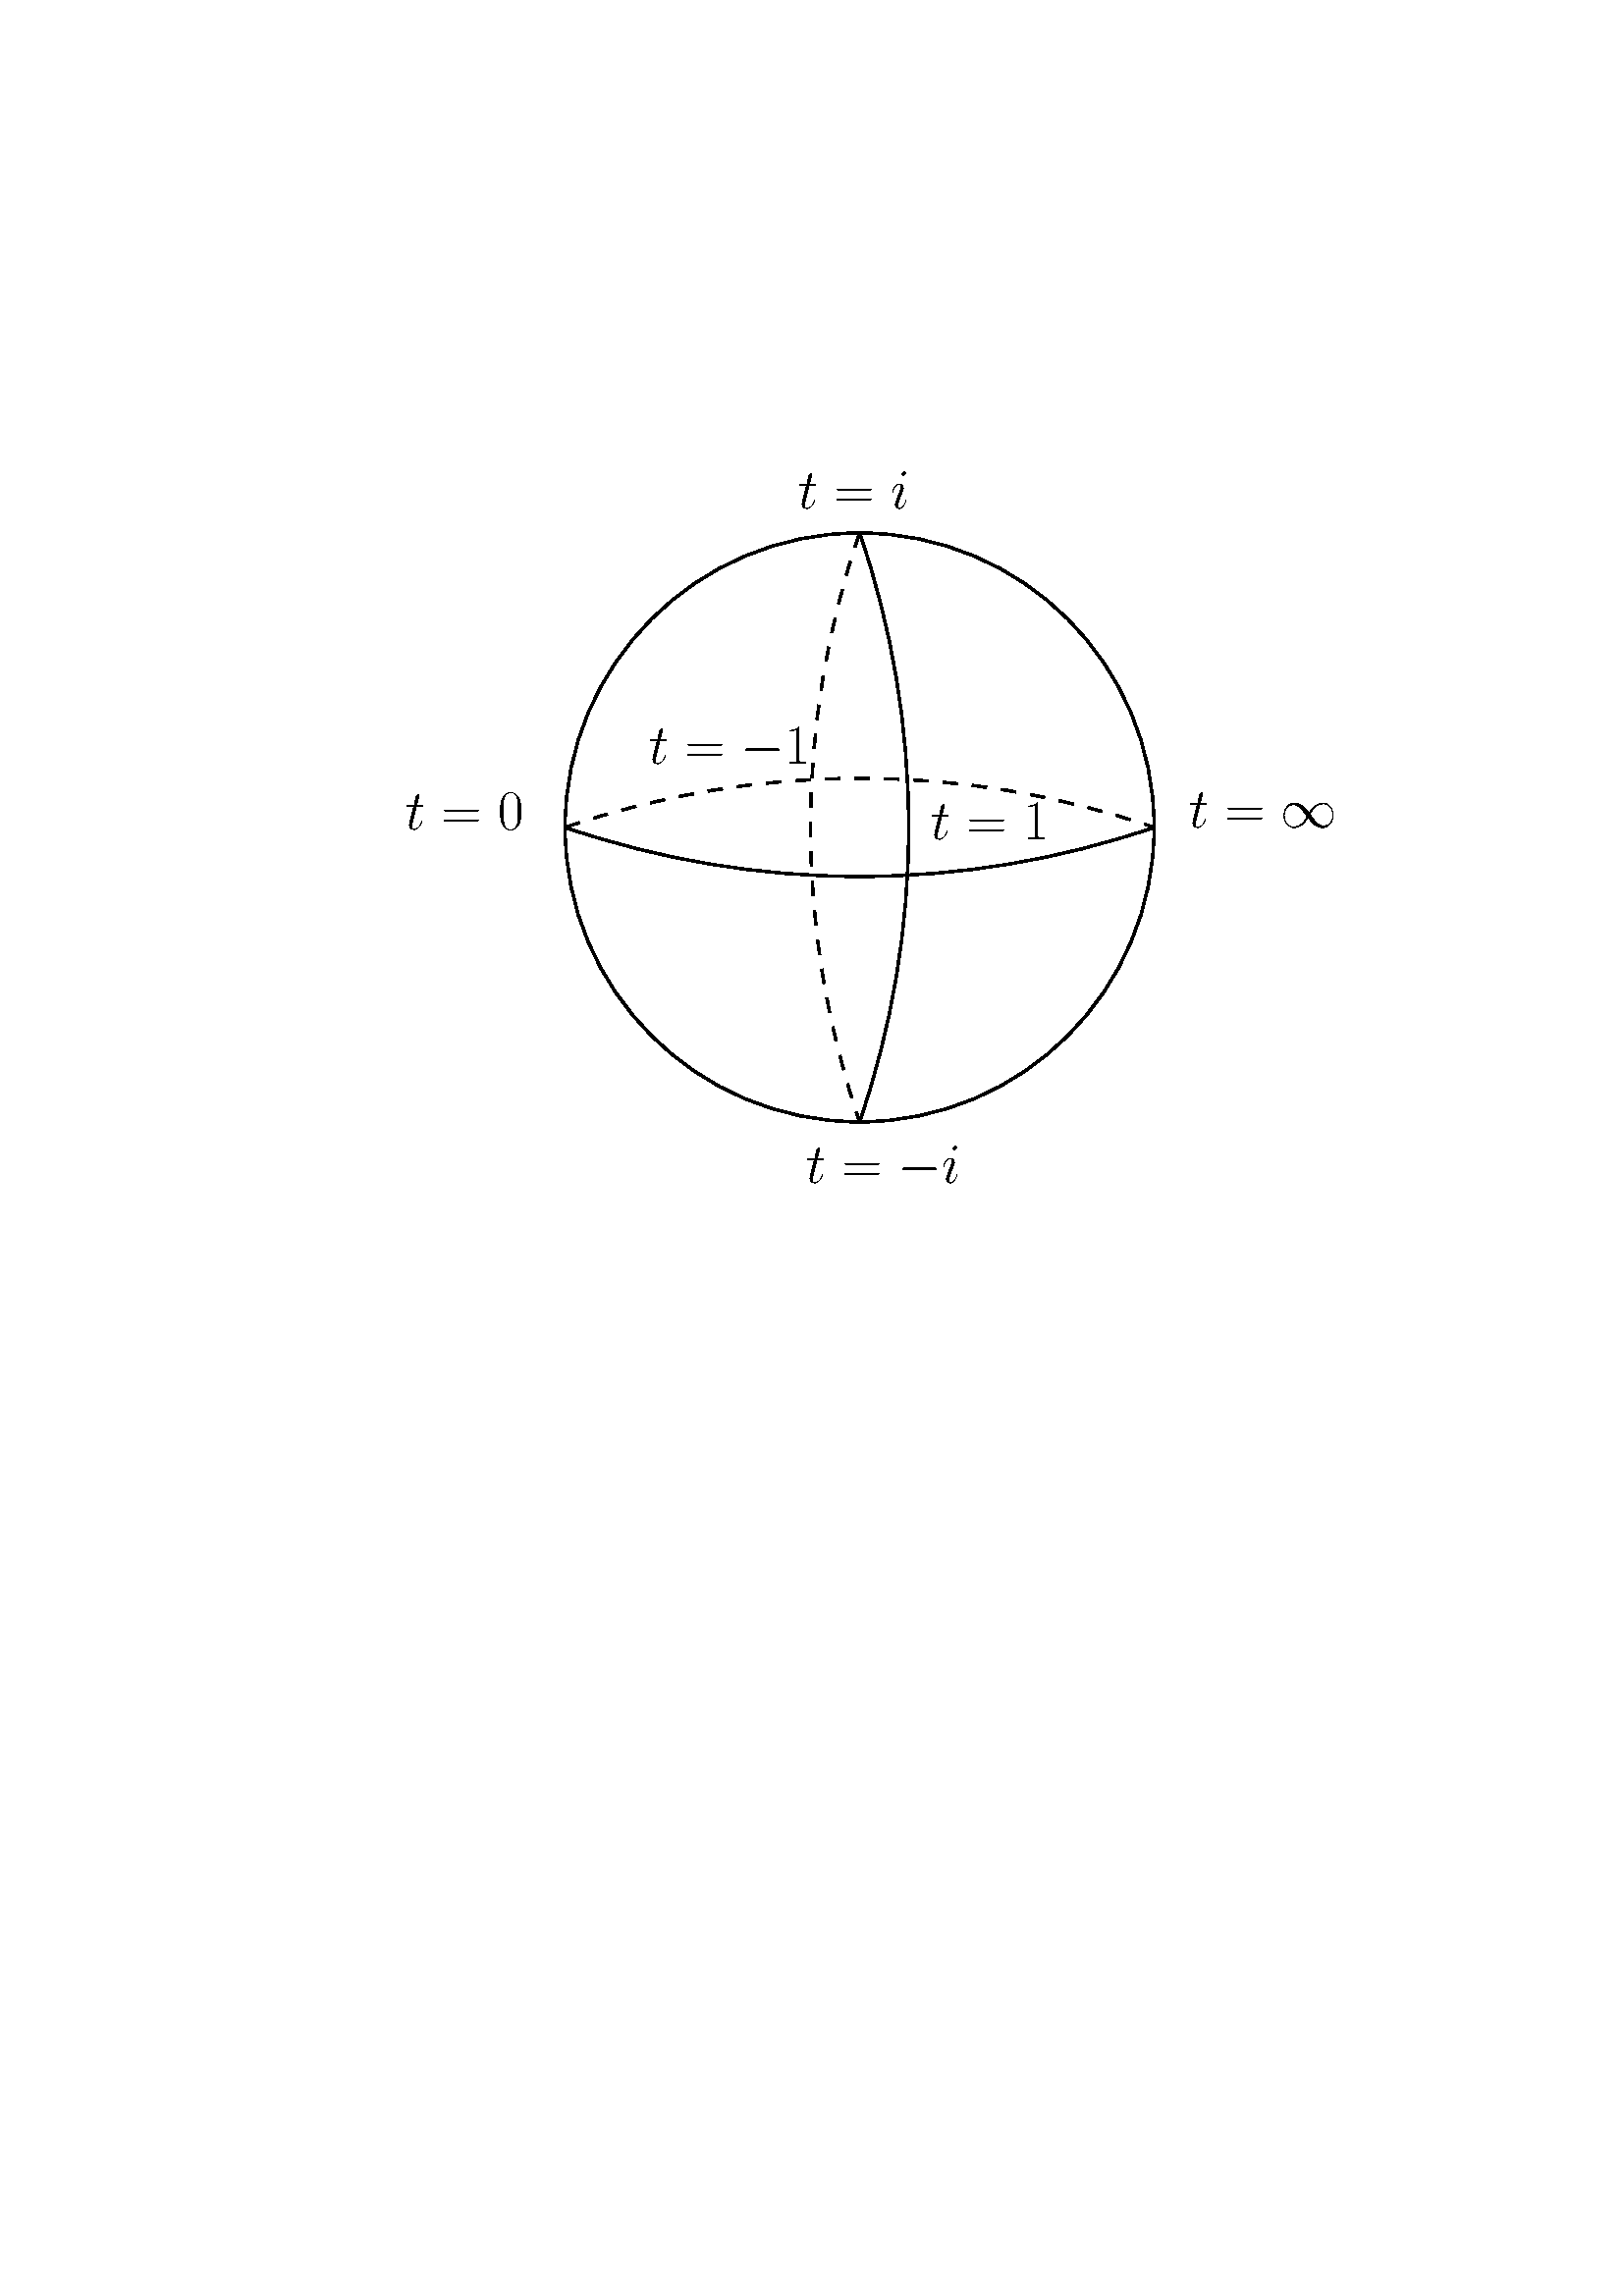
\includegraphics[width=0.75\linewidth]{figures/gla0-1.png}
\caption{ \medskip 以变量 $t$ 为参数的一族拓扑场论。（原文 Fig.~1）}
\label{fig:zunko}
\end{figure}

$Spin'(4)$ 的生成元是 $\Gamma_{\mu\nu}+\Gamma_{\mu+4,\nu+4}$（$\mu,\nu=0,\dots,3$），因此 $Spin'(4)$-不变旋量 $\epsilon$ 满足 $(\Gamma_{\mu\nu}+\Gamma_{\mu+4,\nu+4})\epsilon=0$。取 $\mu,\nu=0,1$，可知 $\Gamma_{0145}\epsilon=\epsilon$；取 $\mu,\nu=2,3$，可知 $\Gamma_{2367}\epsilon=\epsilon$。于是 $\Gamma_0\Gamma_1\dots\Gamma_7\epsilon=\epsilon$；再利用式~\eqref{eq:nohinks} 的手征条件 $\Gamma_0\Gamma_1\dots\Gamma_9\epsilon=-i\epsilon$，可知
% 式 (3.11)
\setcounter{equation}{10}
\begin{equation}\label{eq:banother}
\Gamma_{89}\epsilon=-i\epsilon.
\end{equation}
特别地，由此可知 ${\cal K}=\Gamma_{89}$ 在 $\epsilon_\ell$ 与 $\epsilon_r$ 上以相同的本征值 ${\EUK}=-i{\cal K}=-1$ 作用。还可知 $\Gamma_{8-i9}\epsilon=0$，其中 $\Gamma_{8-i9}=(\Gamma_8-i\Gamma_9)/\sqrt 2$。这些事实有助于验证下文给出的超对称变换律。

现在我们可以看出，为什么这一构造给出以 $\Bbb{CP}^1$ 为参数的一族拓扑场论（\zunko）。我们取 $\epsilon_\ell$ 与 $\epsilon_\rr$ 的任意非零复线性组合 % 式 (3.12)
\setcounter{equation}{11}
\begin{equation}\label{eq:utu}
\epsilon=u\epsilon_\ell+v\epsilon_\rr,
\end{equation}

并把它取作拓扑对称的生成元。对 $\epsilon$ 作整体标度无关紧要，因此拓扑对称的可能选取由 $\Bbb{CP}^1$ 参数化。由于给定 $\epsilon_\ell$ 后 $\epsilon_\rr$ 有自然的选取，这里比一个抽象的 $\Bbb{CP}^1$ 有更多的结构：它带有自然的仿射参数 $t=v/u$。

我们可以用式~\eqref{eq:tokio} 确定 $u$、$v$ 与 $t$ 在 $S$-对偶下的变换。在对偶群 $\Gamma$ 的元素 $\gamma$ 下，有 $\epsilon_\ell\to\exp(i\hat\phi(\gamma))\epsilon_\ell$，$\epsilon_\rr\to\exp(-i\hat\phi(\gamma))\epsilon_\rr$。因此，要保证 $\epsilon=u\epsilon_\ell+v\epsilon_\rr$ 不变，需有 $u\to\exp(-i\hat\phi(\gamma))u$、$v\to\exp(i\hat\phi(\gamma))v$；最终 $t=v/u$ 的变换为

\begin{yizhu}[含糊点拨]
按：式~\eqref{eq:duco} 给出的 $t\mapsto\exp(2i\hat\phi(\gamma))t=\frac{c\tau+d}{|c\tau+d|}t$，与 Frenkel 2009 综述（Séminaire Bourbaki 1010）第 4 节中的 $t\mapsto\frac{\tau}{|\tau|}t$ 相差一个负号：在 $S$-对偶 $\tau\mapsto-1/\tau$ 下，$\frac{c\tau+d}{|c\tau+d|}=\frac{-1/\tau}{1/|\tau|}=-\frac{\tau}{|\tau|}$。两者并不矛盾，因为本文马上就说明 $t$ 与 $-t$ 给出等价的拓扑场论（式~\eqref{eq:ungu}），这个负号被那个平凡等价吸收。记录这一点是因为：不同文献对 twisting parameter 的归一化可能相差一个符号或整体标度，比较公式之前务必先对齐约定。
\end{yizhu} % 式 (3.13)
\setcounter{equation}{12}
\begin{equation}\label{eq:duco}
t\to
\exp(2i\hat\phi(\gamma))t={{c\tau+d}\over\ {|c\tau+d|}}t.
\end{equation}

类似地，我们可以确定 $SU(4)_{{\cal R}}$ 的中心在 $t$ 上的作用。中心的生成元 ${\EUI}$ 按 $\epsilon_\ell\to i\epsilon_\ell$、$\epsilon_\rr\to i^{-1}\epsilon_\rr$ 作用，因此与上面类似的推理给出 % 式 (3.14)
\setcounter{equation}{13}
\begin{equation}\label{eq:ungu}
{\EUI}(t)=-t.
\end{equation}

因此，参数为 $t$ 的拓扑场论与参数为 $-t$ 的拓扑场论彼此等价。这是一种平凡的等价，含义是它来自经典作用量的对称性——而不是来自非平凡的 $S$-对偶。$\Bbb{Z}_2$ 对称性~\eqref{eq:ungu} 是以 $t$ 参数化的一族扭化拓扑场论中唯一的平凡等价。作此断言时，关键的一点是 $\epsilon_\ell$ 与 $\epsilon_\rr$ 具有相同的 ${\cal K}$ 本征值。否则，由 ${\cal K}$ 生成的群 $\Bbb{C}^*$ 中的一个变换将非平凡地作用在 $t$ 上，从而使得整个以 $\Bbb{CP}^1$ 为参数的拓扑场论族都平凡地等价。当然，正因为（几乎）没有平凡等价，来自 $S$-对偶的非平凡等价才有可能生成像几何 Langlands 纲领那样有趣的东西。

\begin{yizhu}[易错点]
按：$t\sim-t$ 是唯一的平凡等价，这句话的分量全在「唯一」二字。理由本段已经给出，但值得用群论重述一遍：如果 $\epsilon_\ell$ 与 $\epsilon_\rr$ 的 ${\cal K}$ 本征值不同，那么由 ${\cal K}$ 生成的连通群 $\Bbb{C}^*$ 会连续地移动 $t$，把 $\Bbb{CP}^1$ 上的每个参数都推入同一个等价类，整族理论随之平凡化，$S$-对偶带来的对偶性也就无从谈起。正因为两者本征值相同（都等于 $-1$，见式~\eqref{eq:banother}），连通的 $\Bbb{C}^*$ 在 $t$ 上作用平凡，只剩下中心元给出的离散 $\Bbb{Z}_2$：$t\mapsto-t$。
\end{yizhu}

我们把由 $\epsilon_\ell$ 与 $\epsilon_\rr$ 生成的超对称记作 $Q_\ell$ 与 $Q_\rr$。由线性组合 $\epsilon=u\epsilon_\ell+v\epsilon_\rr$ 生成的超对称则是 % 式 (3.15)
\setcounter{equation}{14}
\begin{equation}\label{eq:hut}
Q=uQ_\ell+vQ_\rr,
\end{equation}
这就是扭化理论的拓扑对称。写下如下记号也很方便：
% 式 (3.16)
\setcounter{equation}{15}
\begin{equation}\label{eq:nut}
\delta_T=\epsilon_\ell\delta_\ell+\epsilon_\rr\delta_\rr,
\end{equation}

其中对任意场 $\Phi$，
% 式 (3.17)
\setcounter{equation}{16}
\begin{equation}\label{eq:but}
\delta_T\Phi=[Q,\Phi\},~~~\delta_\ell\Phi=
[Q_\ell,\Phi\},~~~\delta_\rr\Phi=[Q_\rr,\Phi\}.
\end{equation}
（$T$ 表示 twisted 或 topological。）由于 $\epsilon_\ell$ 与 $\epsilon_r$ 具有 ${\EUK}=-1$，可知 $Q_\ell$、$Q_\rr$ 与 $Q$ 都具有 ${\EUK}=1$。事实上，下文给出的超对称变换律明确显示，$\delta_T$ 把每个场的 ${\EUK}$ 都提高 $1$。因此在数学语言中，规范不变算子或态构成一个复形，它按 ${\EUK}$ 作 $\Bbb{Z}$-分次，微分是 $Q$。

\begin{yizhu}[易错点]
按：这里的 ${\EUK}$ 记账是全文最容易出错的地方：扭化旋量 $\epsilon_\ell,\epsilon_\rr$ 的 ${\EUK}=-1$，而由它们生成的超荷 $Q_\ell,Q_\rr,Q$ 的 ${\EUK}=+1$；因为 $\delta_T\Phi=[Q,\Phi\}$，$\delta_T$ 把每个场的 ${\EUK}$ 提高 $1$。于是费米场与玻色场的配对不按自旋，而按 ${\EUK}$ 的奇偶：${\EUK}=1$ 的费米场（$\psi,\tilde\psi$）是 $Q$ 的搭档，${\EUK}=-1$ 的（$\chi^\pm,\eta,\tilde\eta$）出现在 $\delta_T$ 的右边。这也解释了为什么 $\sigma$（${\EUK}=2$）在 $\delta_T$ 下不变：要把它映到某个 ${\EUK}=3$ 的场，而理论中没有这样的场。
\end{yizhu}

\par\medskip{\it 费米场与超对称变换}

费米场 $\lambda$ 与超对称生成元 $\epsilon$ 按同样的方式变换，因此利用式~\eqref{eq:lollypop} 与式~\eqref{eq:tollypop}，可以用四维语言识别它们。具有 ${\EUK}=1$ 的场是两个 $({\bf 2},{\bf 2})^1$ 的拷贝，对应两个 1-形式 $\psi$ 与 $\tilde\psi$。按 $({\bf 3},{\bf 1})^{-1}$ 与 $({\bf 1},{\bf 3})^{-1}$ 变换的场，是 ${\EUK}=-1$ 的 2-形式 $\chi$ 的自对偶部分与反自对偶部分 $\chi^\pm$。最后，还有两个 ${\EUK}=-1$ 的零形式 $\eta$ 与 $\tilde\eta$。

为把这些四维场定义得更精确，一个有用的办法是指定十维旋量场 $\lambda$ 按四维费米场的如下展开：\footnote{由于 $\lambda$、$\epsilon_\ell$ 与 $\epsilon_\rr$ 都是正手征的，这一展开只能使用 Clifford 代数的偶元素。为保证这一点，展开中包含若干个因子 $\Gamma_{8+i9}={1\over \sqrt 2}\left(\Gamma_8+ i \Gamma_9\right)$。}
 % 式 (3.18)
\setcounter{equation}{17}
\begin{equation}\label{eq:iko}
\begin{aligned}\lambda=&\left(\eta
+\sum_\mu\Gamma^\mu\psi_\mu \Gamma_{8+i9}
+\sum_{\mu<\nu}\Gamma^{\mu\nu}\chi^+_{\mu\nu}\right)\epsilon_\ell
\\+& \left(\tilde\eta +\sum_{\mu}\Gamma^\mu\tilde\psi_\mu
\Gamma_{8+i9}+\sum_{
\mu<\nu}\Gamma^{\mu\nu}\chi^-_{\mu\nu}\right)\epsilon_\rr.\\\end{aligned}
\end{equation}

这个公式用 $\lambda$ 的十六个分量唯一地确定了十六个场（$\eta$ 与 $\tilde\eta$，$\psi$ 与 $\tilde\psi$ 各四个分量，以及 $\chi$ 的六个分量）。注意，由于 $\hat\Gamma_E\epsilon_\ell=-\epsilon_\ell$，$\Gamma_{\mu\nu}\epsilon_\ell$ 是自对偶的，因此 $\Gamma^{\mu\nu}\chi_{\mu\nu}\epsilon_\ell=\Gamma^{\mu\nu}\chi^+_{\mu\nu}\epsilon_\ell$。同样，$\Gamma^{\mu\nu}\chi_{\mu\nu}\epsilon_\rr=\Gamma^{\mu\nu}\chi^-_{\mu\nu}\epsilon_\rr$。所以在式~\eqref{eq:iko} 中可以把 $\chi^\pm$ 等价地换成 $\chi$。

方便的做法是把 $\epsilon_\ell$ 归一化（允许差一个符号），使得
% 式 (3.19)
\setcounter{equation}{18}
\begin{equation}\label{eq:zomop}
\bar\epsilon_\ell \Gamma_{8+i9}\epsilon_\ell = 1.
\end{equation}
于是由 $\epsilon_r=N\epsilon_\ell$ 同样可得
% 式 (3.20)
\setcounter{equation}{19}
\begin{equation}\label{eq:omop}
\bar\epsilon_r\Gamma_{8+i9}\epsilon_r=1.
\end{equation}
由四维手征性的考虑可得
% 式 (3.21)
\setcounter{equation}{20}
\begin{equation}\label{eq:tomop}
\bar\epsilon_\ell\Gamma_{8+i9}\epsilon_r
=\bar\epsilon_r\Gamma_{8+i9}\epsilon_\ell=0.
\end{equation}

下一步是描述各场在拓扑对称（即由 $\epsilon_\ell$ 与 $\epsilon_\rr$ 生成的超对称）下如何变换。例如，要变换玻色子，我们从 $\delta_S A_I=i\bar\epsilon\Gamma_I\lambda$ 出发。令 $\epsilon=u\epsilon_\ell+v\epsilon_\rr$，就得到四维规范场的变换 % 式 (3.22)
\setcounter{equation}{21}
\begin{equation}\label{eq:kono}
\delta_T A_\mu = iu\bar \epsilon_\ell
\Gamma_\mu \lambda +iv\bar\epsilon_\rr\Gamma_\mu\lambda.
\end{equation}
经过一番 $\Gamma$-矩阵运算，可以得到四维规范场在拓扑超对称下的变换： % 式 (3.23)
\setcounter{equation}{22}
\begin{equation}\label{eq:bono}
\delta_T A_\mu=iu
\psi_\mu+iv\tilde\psi_\mu.
\end{equation}
类似地，对其他玻色场我们得到 % 式 (3.24)
\setcounter{equation}{23}
\begin{equation}\label{eq:lono}
\delta_T\phi_\mu=iv\psi_\mu -
iu\tilde\psi_\mu.
\end{equation}
 % 式 (3.25)
\setcounter{equation}{24}
\begin{equation}\label{eq:otono}
\begin{aligned}\delta_T\sigma & = 0 \\
                       \delta_T\bar\sigma & = iu\eta+iv\tilde\eta.\\\end{aligned}
\end{equation}

$\delta_T\sigma$ 之所以为零，其实只源于 $\sigma$ 具有 ${\EUK}=2$，而并不存在 ${\EUK}=3$ 的合适场。

同样地，我们可以从基本的变换律出发，求出四维费米场的变换：
% 式 (3.26)
\setcounter{equation}{25}
\begin{equation}\label{eq:invo}
\delta_T\lambda=\half\sum_{I,J=0}^9F_{IJ}\Gamma^{IJ}\epsilon,
\end{equation}

其中 $\epsilon=u\epsilon_\ell+v\epsilon_\rr$。具有 ${\EUK}=-1$ 的费米场的变换为
% 式 (3.27)
\setcounter{equation}{26}
\begin{equation}\label{eq:helpme}
\begin{aligned}\delta_T\chi^+ & = u(F-\phi\wedge\phi)^+
+v(D\phi)^+\\ \delta_T\chi^-& = v(F-\phi\wedge\phi)^- -
u(D\phi)^-\\ \delta_T\eta& = vD^*\phi+u[\bar\sigma,\sigma] \\
\delta_T\tilde\eta& = -uD^* \phi+v[\bar\sigma,\sigma].\\\end{aligned}
\end{equation}
具有 ${\EUK}=1$ 的那些场的变换为 % 式 (3.28)
\setcounter{equation}{27}
\begin{equation}\label{eq:mimo}
\begin{aligned}\delta_T\psi& = u\,
D\sigma +v[\phi,\sigma]\\ \delta_T\tilde\psi & = v\, D\sigma - u
[\phi,\sigma].\\\end{aligned}
\end{equation}
在这些公式中，$D=d+[A,\,\cdot \,]$ 是相对于联络 $A$ 的协变导数；在伴随丛取值的 2-形式 $\phi\wedge\phi$ 中隐含着一个李括号；而 $D^*\phi=\star D \star \phi=D_\mu\phi^\mu$，其中 $\star$ 是 Hodge 星算子。

%% ============================================================
%% 分片 06：原文第 3 节「Topological Field Theory From ${\EUN}=4$ Super Yang-Mills Theory」（原文 glshort.tex 起于第 1216 行）
%% 由 tools/harvmac2tex.py 从 arXiv 源码（hep-th/0604151v3）自动生成。
%% 只译英文散文；公式、编号、\label、\cite 一律不改。
%% ============================================================

\subsection{一族 $A$-模型}

\label{sec:familya}

我们处于如下一般情形。我们有一个量子理论，它带有费米对称性 $Q=uQ_\ell+vQ_\rr$，且满足 $Q^2=0$（模一个规范变换）。在这种情形下，路径积分一般会局域化到 $Q$-不变的场上。当 $Q$-不变场的空间 ${\eurm Y}$ 光滑、且规范群在它上面自由作用时，路径积分可以通过在 ${\eurm Y}$ 附近展开的高斯近似或单圈近似来计算。更一般地，也许需要走到更高阶，但路径积分总由 ${\eurm Y}$ 的有限阶无穷小邻域的结构决定。

只需找出 $Q$-不变的玻色场就够了，因为费米场无论如何都是无穷小的，会自动被纳入微扰论。一个玻色场在 $Q$ 下不变的条件是：对每个费米场 $\Psi$，$\delta_T\Psi$ 都为零。换句话说，${\eurm Y}$ 由把式~\eqref{eq:helpme} 与式~\eqref{eq:mimo} 的右边取零来定义。

这些表达式为零这一条件在 $u$ 与 $v$ 的标度变换下不变，因此只依赖于 $t=v/u$。式~\eqref{eq:helpme} 的右边为零给出\footnote{要得到第三个方程，我们在 $t\not=\pm i$ 时取条件 $\delta_T\eta=0$ 与 $\delta_T\tilde\eta=0$ 的一个依赖于 $t$ 的线性组合。$t=\pm i$ 时会怎样，下面再讨论。}

\begin{yizhu}[易错点]
按：脚注里"取 $\delta_T\eta=0$ 与 $\delta_T\tilde\eta=0$ 的 $t$-依赖线性组合"这句话，是理解式~\eqref{eq:loopme} 中第三条方程 $D^*\phi=0$ 来历的关键。直接由式~\eqref{eq:helpme} 令 $\delta_T\eta=0$ 与 $\delta_T\tilde\eta=0$，得到的是 $vD^*\phi+u[\bar\sigma,\sigma]=0$ 与 $-uD^*\phi+v[\bar\sigma,\sigma]=0$；把两式按适当系数组合消去 $[\bar\sigma,\sigma]$，就得到 $D^*\phi=0$，但组合系数的行列式正比于 $u^2+v^2$，故只在 $t^2\not=-1$（即 $t\not=\pm i$）时可以这样做。$t=\pm i$ 时这两式线性相关，只能得到 $D^*\phi\pm i[\bar\sigma,\sigma]=0$，这正是后文在式~\eqref{eq:toopme} 之后特别说明的情形。
\end{yizhu}
% 式 (3.29)
\setcounter{equation}{28}
\begin{equation}\label{eq:loopme}
\begin{aligned}(F-\phi\wedge\phi+tD\phi)^+ & = 0
\\
                      (F-\phi\wedge\phi-t^{-1}D\phi)^-& = 0 \\
                      D^* \phi & = 0.\\\end{aligned}
\end{equation}

对这些方程最初步的解释是取 $-t^{-1}=t$，或等价地 $t=\pm i$。对几何 Langlands 纲领很重要的正是这些 $t$ 值；此时令 ${\cal A}$ 为 ${G}_{\Bbb{C}}$ 取值的联络 ${\cal A}=A+i\phi$，其曲率为 ${\cal F}=d{\cal A}+{\cal A}\wedge{\cal A}$。于是式~\eqref{eq:loopme} 的前两个方程等价于 ${\cal F}=0$，从而 $t=\pm i$ 时式~\eqref{eq:loopme} 的解给出一个复值平坦联络，进而给出同态 $\pi_1(M)\to G_{{\Bbb{C}}}$。式~\eqref{eq:loopme} 还要求我们再添上条件 $D^*\phi=0$，并模去 $G$ 取值的规范变换。把这两步合起来，就构造出同态 $\vartheta:\pi_1(M)\to {{{G}}}_{\Bbb{C}}$ 的模空间 ${\cal Y}$（需要更明确时，我们把这个空间记作 ${\cal Y}_M$ 或 ${\cal Y}_M(G)$）。

\begin{yizhu}[含糊点拨]
按：为什么 $t=\pm i$ 时前两个方程合起来就是 ${\cal F}=0$？要点是：当 $-t^{-1}=t$ 时，$(F-\phi\wedge\phi+tD\phi)^+=0$ 与 $(F-\phi\wedge\phi+tD\phi)^-=0$ 恰好是同一个复方程 $F-\phi\wedge\phi+iD\phi=0$ 的自对偶投影与反自对偶投影；把 ${\cal A}=A+i\phi$ 的曲率展开，${\cal F}=F+iD\phi-\phi\wedge\phi$，正是这个组合。这一步是整套构造的关键：它把"扭化后的 BPS 方程"变成"平坦联络方程"，从而把四维规范场论与二维的 Higgs 丛/平坦丛语言连接起来。注意 $t=i$ 与 $t=-i$ 分别对应 ${\cal A}$ 与 $\bar{\cal A}$，具体哪个对应哪个取决于 $\phi$ 的符号约定；后文在讨论 $t$ 与 $-t$ 等价处还会回到类似的符号问题。
\end{yizhu}
这一陈述依赖于 Corlette 的一个定理 \cite{ref58}（二维情形也由 Donaldson 在 \cite{ref20} 的附录中证明）：对 $(A,\phi)$ 模去 $G$ 取值的规范变换、要求 ${\cal F}=0$ 并加上 $D^*\phi=0$，等价于直接去掉最后一个方程、只要求 ${\cal F}=0$ 以及一个稳定性条件\footnote{正如涉及 $G_{\Bbb{C}}$ 这类非紧对称群的模问题通常那样，模空间 ${\cal Y}_M(G)$ 并不字面地参数化 $\pi_1(M)\to G_{\Bbb{C}}$ 的所有共轭类。要得到好的模空间，必须去掉某些「不稳定轨道」，在这类问题里它们对应于可约化为三角形式但不能约化为直和的和同态。取 $D^*\phi=0$ 并模去 $G$ 取值的规范变换恰好去掉这些不稳定轨道，这一点在 \cite{ref58} 中得到了证明。关于稳定性所起的作用，我们在第~\ref{sec:complexstr}~节有更充分的说明。}，并模去 $G_{\Bbb{C}}$ 取值的规范变换群。

更一般地，若 $t$ 不是实数，则对取值于 $G$ 的实李代数的场 $A,\phi$，方程~\eqref{eq:loopme} 是超定的而非椭圆型的。把这些方程的厄米部分与反厄米部分分别取零，即可知对任何非实 $t$，它们都推出 ${\cal F}=0$。

然而我们想弄清楚当 $t$ 为实数时会发生什么。（对几何 Langlands 纲领最重要的 $t$ 值是 $t=\pm i$ 与 $t=\pm 1$。）此时方程是实的，我们得到一族以 $t$ 为参数的实椭圆方程。按字面写法，这些方程在 $t\not=0,\infty$ 时是正则的。不过，由式~\eqref{eq:helpme} 右边的齐次表达式可以看出，通过把第二个方程乘以 $t$、或把第一个方程乘以 $t^{-1}$，方程可以延拓到 $t=0$ 或 $t=\infty$。于是在 $t=0$ 处，我们应把第二个方程换成 $(D\phi)^-=0$；在 $t=\infty$ 处，把第一个方程换成 $(D\phi)^+=0$。这样便得到一族以 $\Bbb{RP}^1$ 为参数的实椭圆方程。

我们可以类似地理解来自式~\eqref{eq:mimo} 的未破缺超对称条件：
 % 式 (3.30)
\setcounter{equation}{29}
\begin{equation}\label{eq:toopme}
\begin{aligned}D\sigma + t[\phi,\sigma]& = 0\\
                     D\sigma - t^{-1}[\phi,\sigma]& = 0.\\
                     \end{aligned}
\end{equation}

对任何不等于 $\pm i$ 的 $t$，这些方程都推出 $D\sigma=[\phi,\sigma]=0$；这个条件意味着由 $\sigma$ 生成的规范对称保持~\eqref{eq:loopme} 的给定解不变。
此外，当 $t\not=\pm i$ 时，把方程 $\delta_T\eta=0$ 与 $\delta_T\tilde\eta=0$ 作一个线性组合便给出
% 式 (3.31)
\setcounter{equation}{30}
\begin{equation}\label{eq:woopem}
[\sigma,\bar\sigma]=0.
\end{equation}

只要我们只考虑不可约的超对称场——或者更一般地，考虑自同构群有限的超对称场——式~\eqref{eq:toopme} 就推出 $\sigma=0$。本文一般只考虑不可约的超对称场。关于可约情形的若干简单注记将出现在 \cite{ref26} 中。

在 $t=\pm i$ 处结论类似，只是细节不同。此时式~\eqref{eq:toopme} 说的是：$\sigma$ 生成平坦 $G_\Bbb{C}$ 值联络 $\CA$ 或 $\bar\CA$ 的一个对称。同样，只要只考虑不可约的超对称场，就可以假设 $\sigma=0$。（对 $t=\pm i$，若存在带 $\sigma\not=0$ 的可约超对称位形，我们得不到分离的条件 $D^*\phi=[\sigma,\bar\sigma]=0$，而只有线性组合 $D^*\phi\pm i[\sigma,\bar\sigma]=0$。）

对实 $t$，这里讨论的理论属于上同调场论 \cite{ref59} 的一般框架，就像四维的 Donaldson 理论或二维的 $A$-模型。场是具有 ${\EUK}=0$ 的玻色场 $A,\phi$；方程是~\eqref{eq:loopme}；对称性就是规范对称性。与任何这类理论一样，在没有算子插入时，路径积分可以通过对方程的解带符号计数来计算，只要这些解是孤立且不可约的。一个给定解的贡献符号，就是相应的单圈费米子行列式的符号。由空间 ${\eurm Y}_0$（它是 ${\eurm Y}$ 的一个分支）参数化的一族光滑紧的不可约解，其贡献是 ${\eurm Y}_0$ 的 Euler 示性数加上或减去一个符号，符号仍然来自费米子行列式。${\eurm Y}$ 中奇点的贡献以及可约解的贡献——例如 $A=\phi=0$ 的平凡解——更微妙，这里不予考虑。

由于带符号加权的解的数目在椭圆方程族的连续形变下不变，闭四维流形上无算子插入的配分函数必定与 $t$ 无关，至少对实 $t$ 如此。由全纯性，这对复 $t$ 也成立。闭四维流形上的配分函数与 $t$ 无关这一点，也可以更直接地从路径积分看出，后文会解释。从数学观点看，第~\ref{sec:vanishing}~节的消灭定理将给出关于 $t$-无关性的强陈述：式~\eqref{eq:loopme} 的解空间实际上与 $t$ 无关，$t=0,\infty$ 除外。

参数 $t$ 的重要性在于：可以引入一些算子，或者当 $M$ 有边界时引入一些边界条件，它们只在某个特定的 $t$ 值下保持拓扑对称性。与 Donaldson 理论一样，这里考虑的 TQFT 具有保持拓扑对称性的局部算子。这些算子在 \cite{ref53,ref54,ref55,ref56,ref57} 中讨论过，并将另文进一步分析 \cite{ref26}。然而，它们并不是几何 Langlands 纲领中最重要的算子。最重要的算子是第~\ref{sec:loopop}~节引入的 Wilson 与 't Hooft 线算子，它们在更熟悉的上同调场论中没有明显的近亲。

如果我们在实 $t$ 时的理论多少类比于二维 $A$-模型，那么复 $t$ 时它对应于什么？$t=\pm i$ 处的理论类比于二维 $B$-模型。在描述从黎曼面 $\Sigma$ 到复流形 $X$ 的映射 $\Phi:\Sigma\to X$ 的 $B$-模型中，超对称场是 $\Sigma$ 到 $X$ 的常映射。两种情形之间明显的相似之处是：常映射或平坦的 $G_{\Bbb{C}}$ 值联络都相对容易用超定方程（而非椭圆方程）描述——前者是 $d\Phi=0$，后者是 ${\cal F}=0$——而其中的复结构是显然的。当我们于第~\ref{sec:compacthitchin}~节考虑维数约化时，将会看到更深刻的类比。

\begin{yizhu}[物理图像]
按：把实 $t$ 与 $t=\pm i$ 两端对照起来看，本节给出了一个很有用的三分法：$t=\pm i$ 时方程是复的、超定的，解是平坦 $G_{\Bbb{C}}$ 值联络（类比二维 $B$-模型）；实 $t$ 时方程是实椭圆型的，路径积分按解的带符号计数给出（类比二维 $A$-模型，或四维 Donaldson 理论）；而 $t=0,\infty$ 是两个端点，方程退化，但通过乘以 $t$ 或 $t^{-1}$ 仍有意义（见式~\eqref{eq:loopme} 之后的讨论）。原文只谨慎地说这样得到的理论"松散地说是拓扑场论"，因为它可能依赖 $M$ 的光滑结构；但无论如何，$t$ 是这个理论族中唯一本质的参数（除 $t\sim-t$ 外），这也是为什么 $S$-对偶作用在 $t$ 上能产生非平凡的对偶性。
\end{yizhu}

\subsection{消灭定理}

\label{sec:vanishing}

令 $\EUV^+(t)= (F-\phi\wedge\phi+tD\phi)^+$、$\EUV^-(t)= (F-\phi\wedge\phi-t^{-1}D\phi)^-$、$\EUV_0= D^* \phi$，则超对称方程是 $\EUV^+(t)=\EUV^-(t)=\EUV_0=0$。本节我们集中讨论 $t$ 为实数的情形，此时超对称方程是椭圆型的。

与许多同超对称相联系的一阶方程一样——例如全纯曲线方程、Yang--Mills 瞬子方程、Seiberg--Witten 方程，或 \cite{ref45} 中研究的方程——这些方程受制于不寻常的消灭定理。在目前的情形，我们有：

\par\medskip
 {\it 消灭定理 1~}  设 $M$ 为紧的无边四维流形，$E$ 为 $M$ 上的 $G$-丛，其 Pontryagin 类非零，即 $\int_M\Tr\,F\wedge F\not=0$。那么对任何 $t\not=0,\infty$，超对称方程 $\EUV^+(t)=\EUV^-(t)=\EUV_0=0$ 无解。

\par\medskip  {\it 消灭定理 2~} 在这样的 $M$ 上，任何对某个不为 $0,\infty$ 的 $t$ 值满足这些方程的场，对一切 $t$ 都满足这些方程，因而由一个平坦的 $G_\Bbb{C}$ 值联络给出。

\begin{yizhu}[易错点]
按：消灭定理 1 是关于固定丛 $E$ 上的经典方程无解的陈述，而不是关于配分函数的陈述：它说的是对任意 $t\not=0,\infty$，方程 $\EUV^\pm(t)=\EUV_0=0$ 在 $E$ 上根本没有解，因此配分函数为零。这类"一阶方程 + 非零拓扑荷"的消灭现象在超对称方程中很常见（全纯曲线、Yang--Mills 瞬子、Seiberg--Witten 方程都有类似结论），其共同机制是把方程写成平方和等于拓扑荷的形式（见式~\eqref{eq:hombo} 与式~\eqref{eq:ormob}）：若平方和为零而拓扑荷非零，就不可能。定理 1 的证明只在 $t\not=0,\infty$ 有效，而 $t=0,\infty$ 处确实有解，这一点下文会说明。
\end{yizhu}

\par\medskip

第一个消灭定理的最短证明来自如下恒等式： % 式 (3.32)
\setcounter{equation}{31}
\begin{equation}\label{eq:hombo}
\int_M\Tr\,F\wedge
F=\int_M\Tr\left(\EUV^+(t)\wedge \EUV^+(-t^{-1})+\EUV^-(t)\wedge
\EUV^-(-t^{-1})\right).
\end{equation}
这个恒等式的证明是直接的，用到分部积分。显然，这个恒等式说明：若对某个 $t$ 有 $\EUV^\pm(t)=0$，则 $\int_M\Tr\, F\wedge F=0$。

当 $t=0,\infty$ 时，由于 $\EUV^\pm$ 的极点，这个证明失效。事实上，$t=0,\infty$ 时结论确实不成立：$t=0$ 或 $t=\infty$ 的方程至少有明显的解，即取 $\phi=0$ 的瞬子或反瞬子。

对第二消灭定理，我们需要一个类似但更复杂的恒等式： % 式 (3.33)
\setcounter{equation}{32}
\begin{equation}\label{eq:ormob}
\begin{aligned}&-\int_Md^4x\sqrt
g\,\Tr\,\left({t^{-1}\over
t+t^{-1}}\EUV^+(t)_{\mu\nu}\EUV^+(t)^{\mu\nu}+{t\over
t+t^{-1}}\EUV^-(t)_{\mu\nu}\EUV^-(t)^{\mu\nu}+\EUV_0^2\right)\\
&=-\int d^4x\sqrt g\,\Tr\,\left({1\over 2}F_{\mu\nu}
F^{\mu\nu}+D_\mu\phi_\nu D^\mu\phi^\nu
+R_{\mu\nu}\phi^\mu\phi^\nu+ {1\over
2}[\phi_\mu,\phi_\nu]^2\right)\\&~~~~~~~+{t-t^{-1}\over
(t+t^{-1})}\int_M\Tr\, F\wedge F. \\\end{aligned}
\end{equation}
这个恒等式令人惊讶之处在于：除了一项正比于 $\int\,\Tr\,F\wedge F$ 的拓扑不变量之外，右边与 $t$ 无关。其证明类似于式~\eqref{eq:hombo} 的证明，但更繁复。$R_{\mu\nu}$ 是 $M$ 的 Ricci 张量，它出现在把 $\int_Md^4x\sqrt g D_\mu\phi_\nu D^\nu\phi^\mu$ 与 $\int d^4x\sqrt g (D_\mu\phi^\mu)^2$ 联系起来的分部积分中。与式~\eqref{eq:hombo} 不同，式~\eqref{eq:ormob} 在 $t\to 0,\infty$ 时有自然的极限：只需把 $t (\EUV^-)^2/(t+t^{-1})$ 换成 $\lim_{t\to 0}(t\EUV^-)^2$，或把 $t^{-1}(\EUV^+)^2/(t+t^{-1})$ 换成 $\lim_{t\to \infty}(t^{-1}\EUV^+)^2$。因此基于式~\eqref{eq:ormob} 的论证在 $t=0,\infty$ 处也成立。

\begin{yizhu}[含糊点拨]
按：式~\eqref{eq:ormob} 是消灭定理的技术核心，值得看清它的结构：左边是 $-\int\sqrt g\,\Tr(\text{三组平方项})$，右边是 $-\int\sqrt g\,\Tr(\text{与 $t$ 无关的"能量"})$ 加上 $f(t)\int\Tr F\wedge F$。也就是说，两边之差给出了一个正比于拓扑荷的项，这是"对 $t$ 的依赖只能来自拓扑项"这一事实的定量形式；正因如此，$t\to 0,\infty$ 的极限存在，论证可以覆盖端点。它本质上是 Bogomolny 型平方和恒等式的高维版本，与四维瞬子方程、二维 $A$-模型的能量恒等式同源。第~\ref{sec:toplag}~节会通过超对称作用量的 $Q$-恰当分解给出它的物理解释。
\end{yizhu}

在第~\ref{sec:toplag}~节，我们将理解式~\eqref{eq:ormob} 的物理意义。现在，我们只用它来完成消灭定理的证明。

为证明第二消灭定理，我们必须证明：若丛 $E$ 上存在一对 $A,\phi$，使得对某个不为 $0,\infty$ 的 $t$ 值有 $\EUV^\pm(t)=\EUV_0=0$，则这些方程对一切 $t$ 都成立。我们已经知道，在这样的解中 $\int_M\Tr\,F\wedge F=0$，因此式~\eqref{eq:ormob} 的右边与 $t$ 无关。于是若左边对某个 $t$ 值取零，则它对一切 $t$ 都取零。此外，左边是平方和，因此对给定的 $t$，它取零当且仅当 $\EUV^\pm(t)=\EUV_0=0$。再者，如我们已经注意到的，$\EUV^\pm(t)$ 与 $\EUV_0$ 对一切 $t$ 取零，等价于 $G_{\Bbb{C}}$ 值联络 ${\cal A}=A+i\phi$ 的曲率 ${\cal F}=d{\cal A}+{\cal A}\wedge{\cal A}$ 取零。这就完成了论证。

最后，我们可以用式~\eqref{eq:ormob} 证明第一消灭定理的一个稍强版本：

\par\medskip{\it 消灭定理 1$'$~} 当 $\int_M\Tr\,F\wedge F>0$ 时，超对称方程除 $t=0$ 外无解；当 $\int_M\Tr\,F\wedge F<0$ 时，除 $t=\infty$ 外无解。\par\medskip

令 ${\eurm B}(t)$ 记式~\eqref{eq:ormob} 的左边，并令 $f(t)=(t-t^{-1})/(t+t^{-1})$。对任意 $t,u$，我们有
% 式 (3.34)
\setcounter{equation}{33}
\begin{equation}\label{eq:toto}
{\eurm B}(u)-{\eurm B}(t)=(f(u)-f(t))\int_M\Tr \,F\wedge
F.
\end{equation}
若 $\EUV^\pm(t)=\EUV_0=0$，则 ${\eurm B}(t)=0$；又因函数 ${\eurm B}$ 是正半定的，式~\eqref{eq:toto} 的左边是正半定的。为使右边正半定，若 $\int_M\Tr\,F\wedge F>0$，$t$ 必须是函数 $f$ 的最小值点；若 $\int_M\Tr\,F\wedge F<0$，$t$ 必须是最大值点。而唯一的最小值在 $t=0$，唯一的最大值在 $t=\infty$。

\begin{yizhu}[原文疑误]
按：这里有一个符号疑点，值得记录。式~\eqref{eq:ormob} 的左边显含一个负号，括号内的量对 $t\not=0$ 是正的平方和（系数的正负可直接验证），所以按字面计算 ${\eurm B}(t)\le 0$，即 ${\eurm B}$ 是负半定的；但本段接着说 ${\eurm B}$ 是正半定，并用"正半定"推理两次，最后得出 $t=0$ 为最小值点——定理 1$'$ 的陈述也与此一致。已核对的 arXiv 源文与已出版版本（PDF 第 31 页）此处均写作 positive semidefinite，故这是原文自身的符号不一致，而非抄录错误：要么式~\eqref{eq:ormob} 左边的负号应当去掉，要么"正半定/最小/最大"这串推理应整体取反。两种改法给出的 $\int\Tr F\wedge F$ 符号与 $t=0,\infty$ 的对应关系并不相同，读者若要引用该结论，宜先按自己的符号约定把式~\eqref{eq:ormob} 重新验算一遍。本书照原文逐字译出，未在正文改动。
\end{yizhu}

\par\medskip{\it 关于紧化的一个注记}

消灭定理的一个特例与紧化有关。我们取 $M=\Sigma\times C$，其中 $\Sigma$ 与 $C$ 是紧黎曼面。在我们的应用中，$C$ 是研究几何 Langlands 纲领所在的黎曼面，而我们把 $\Sigma$ 想成比 $C$ 大得多。不过在拓扑场论中，$\Sigma$ 与 $C$ 上的度规都无关紧要。

对 $t\not=0,\infty$，第二消灭定理说 $M$ 上超对称方程的任何解都由一个平坦的 $G_{\Bbb{C}}$ 值联络给出。$M=\Sigma\times C$ 上的平坦丛 $E$ 有分解\footnote{在这段讨论中，为简单起见我们使用向量丛的语言，就像 $G=SU(N)$ 一样。要把论证推广到任意 $G$，只需改用 $G$ 的子群而不是 $E$ 的子丛来表述即可。} $E=\oplus_{i=1}^n E'_i\otimes E''_i$，其中 $E'_i$ 是从 $\Sigma$ 拉回的平坦丛，$E''_i$ 是从 $C$ 拉回的平坦丛。

\begin{yizhu}[物理图像]
按：这个分解是本节与后文（第~\ref{sec:compacthitchin}~节）之间的桥梁，值得记住它的几何含义：$M=\Sigma\times C$ 上的平坦丛可以拆成"沿 $\Sigma$ 方向"与"沿 $C$ 方向"两部分的直和；限制到一点 $x\in\Sigma$ 之后，剩下的只是 $C$ 上的平坦丛 $E_x$，它正是 Hitchin 模空间 ${\MH}$ 中的一个点。于是 $\Sigma\times C$ 上的超对称场给出映射 $\Sigma\to{\MH}$；在 ${\EUN}=4$ 与 $S$-对偶的图景中，这正是四维理论紧化到二维后靶空间为 Hitchin 模空间的 sigma 模型的开端。Witten 2008 综述在讨论 Hitchin 纤维化与镜像对称时用的也是这套语言。
\end{yizhu}

若我们限制到一点 $x\in \Sigma$，则 $E'_i$ 变为平凡的。若 $d_i$ 是 $E_i'$ 的秩，则 $E$ 约化为 $E_x=\oplus_{i=1}^n d_iE''_i$，即从 $C$ 拉回的平坦丛的直和。$E_x$ 是 $C$ 上的平坦丛，因此定义了 Hitchin 模空间 ${\MH}$ 中的一个点；我们将在第~\ref{sec:compacthitchin}~节更充分地描述该模空间。眼下，我们可以就把 ${\MH}$ 想成 $C$ 上平坦 $G_\Bbb{C}$-丛的模空间。于是 $\Sigma\times C$ 上的任何超对称场都由一个从 $\Sigma$ 到 ${\MH}$ 的映射给出，即 $x\to E_x$。

模空间 ${\MH}$ 有对应于可约平坦丛的奇点。在当前的构造中，当 $n>1$ 时丛 $E_x$ 是可约的。对 $n=1$，有 $E=E'\otimes E''$，其中两个因子分别是从 $\Sigma$ 与 $C$ 拉回的。除非 $E'$ 的秩为 $1$（此时对 $G=SU(N)$ 它必为平凡的），$E_x$ 仍是可约的。因此，避开 ${\MH}$ 奇点的情形，恰好是 $E$ 为某个不可约平坦丛 $E''\to C$ 的拉回的情形。

超对称场同时也是使作用量取极小的位形；这一点在我们于第~\ref{sec:toplag}~节构造超对称拉格朗日量时就会清楚。在上述推理中，我们取 $\Sigma$ 与 $C$ 为紧的。在我们的应用里，我们也关心 $\Sigma$ 为完备但非紧的二维流形的情形，例如 $\Bbb{R}^2$、$\Bbb{R}^2_+$ 或 $\Bbb{R}\times I$（其中 $\Bbb{R}^2_+$ 是半空间，$I$ 是闭区间）。只要给定适当的边界条件与无穷远处的渐近行为，使得第二消灭定理的证明得以成立，这些情形下超对称场仍有分解 $E=\oplus_{i=1}^nE'_i\otimes E''_i$。（当 $\Sigma$ 平坦且单连通时，我们所说的 $E'_i$ 指带有平凡联络与协变常值 Higgs 场的丛。）由此得到与紧 $\Sigma$ 时相同的结论：避开 ${\MH}$ 奇点的超对称场是来自 $C$ 的拉回。

%% ============================================================
%% 分片 07：原文第 3 节「Topological Field Theory From ${\EUN}=4$ Super Yang-Mills Theory」（原文 glshort.tex 起于第 1216 行）
%% 由 tools/harvmac2tex.py 从 arXiv 源码（hep-th/0604151v3）自动生成。
%% 只译英文散文；公式、编号、\label、\cite 一律不改。
%% ============================================================

\subsection{拓扑拉格朗日量}

\label{sec:toplag}

现在我们的目标是找到一个拉格朗日量：它对任意 $t$ 值都具有拓扑对称，并且在 $M$ 平坦时退化为底层 ${\EUN}=4$ 超对称杨--米尔斯理论的拉格朗日量。我们可以手工来做这件事——从平坦 $M$ 下的式~\eqref{eq:ygo} 出发，追问当 $M$ 不再平坦时，需要哪些依赖于曲率的项才能保持拓扑对称。但我们将采取另一种途径。

一个非常有用的第一步，是计算超对称 $Q_\ell$ 与 $Q_\rr$ 在场上生成的代数；等价地，计算 $Q=uQ_\ell+vQ_\rr$ 生成的代数。对场 $A,\phi,\psi$、$\tilde\psi$ 与 $\sigma$，我们算得
% 式 (3.35)
\setcounter{equation}{34}
\begin{equation}\label{eq:ibo}
\begin{aligned}\delta_T{}^2 A & = -i(u^2+v^2)(-D\sigma)\\
\delta_T{}^2\phi & = -i(u^2+v^2)[\sigma,\phi]\\ \delta_T{}^2 \psi
& = -i(u^2+v^2)[\sigma,\psi]\\ \delta_T{}^2\tilde\psi& =
-i(u^2+v^2)[\sigma,\tilde\psi]\\ \delta_T{}^2\sigma& = 0.\\\end{aligned}
\end{equation}

这些结果可以概括为：若 $\Phi$ 是任何 $\EUK\geq 0$ 的场，则 $\delta_T{}^2\Phi=-i(u^2+v^2){{\lie}}_\sigma(\Phi)$，其中 ${{\lie}}_\sigma(\Phi)$ 是 $\Phi$ 在由 $\sigma$ 生成的规范变换下的一阶变化（因此 $\lie$ 代表 Lie 导数）。例如 ${{\lie}}_\sigma(A)=-D\sigma$；对此处的其他场，${{\lie}}_\sigma(\Phi)=[\sigma,\Phi]$。关系式 $\delta_T{}^2\Phi=-i(u^2+v^2){{\lie}}_\sigma(\Phi)$ 可以按 $u$ 与 $v$ 的幂展开，它等价于
% 式 (3.36)
\setcounter{equation}{35}
\begin{equation}\label{eq:uvu}
\begin{aligned}\delta_\ell^2\Phi=\delta_r^2\Phi&=-i{{\lie}}_\sigma(\Phi)\\
\{\delta_\ell,\delta_\rr\}\Phi& = 0.\\\end{aligned}
\end{equation}

然而，若对 $\EUK<0$ 的场计算 $\delta_T{}^2\Phi$，并不能以显然的方式得到 $-i(u^2+v^2){{\lie}}_\sigma(\Phi)$。事实上，在扭化后的 ${\EUN}=4$ 超对称杨--米尔斯理论中，关系式 $\delta_T{}^2\Phi=-i(u^2+v^2){{\lie}}_\sigma(\Phi)$ 对所有 $\Phi$ 都成立；但对某些场，它只有在用到运动方程时才成立。

\begin{yizhu}[易错点]
按：(3.35) 给出的代数对 $\EUK\geq 0$ 的场无需运动方程即成立。$\EUK$ 是扭化所用的那个 $U(1)$ 荷（第~\ref{sec:twisting}~节已逐个标定各场取值）：$A$ 与 $\phi$ 的 $\EUK=0$，$\psi$ 与 $\tilde\psi$ 的 $\EUK=1$，$\chi,\eta,\tilde\eta$ 的 $\EUK=-1$，而 $\sigma$ 的 $\EUK=2$、$\bar\sigma$ 的 $\EUK=-2$；相应地，$\delta_T$ 每作用一次便把 $\EUK$ 提高 1。$\sigma$ 位于最高处，$[\sigma,\sigma]=0$ 使 (3.35) 的最后一行 $\delta_T{}^2\sigma=0$ 与通式自洽；反过来，对 $\EUK<0$ 的 $\chi,\eta,\tilde\eta$，其变换含 $\sigma$ 以外的非线性项，代数在壳外并不闭合，这正是下一段需要辅助场的根源。
\end{yizhu}

一般说来，构造超对称拉格朗日量要容易得多，只要能够引入「辅助场」——它们是额外的场，若愿意，最终可以用其运动方程消去；引入它们的目的是让代数（在这里即 $\delta_T{}^2\Phi=-i(u^2+v^2){{\lie}}_\sigma(\Phi)$）无需借助运动方程便得到满足。在具有大量超对称的理论（例如 ${\EUN}=4$ 超对称杨--米尔斯理论）中，要找到合适的辅助场可能非常困难。正如 \cite{ref53} 首先指出的那样，本例正是这一问题出现的情形。

不过，这一困难可以通过引入一个辅助场 $P$ 而大大缓解：$P$ 是取值于李代数的零形式，引入它是为了让 $\eta$ 与 $\tilde\eta$ 的代数闭合（但不包括 $\chi$）。我们取 $\bar\sigma,\eta,\tilde\eta$ 与 $P$ 的变换律为
% 式 (3.37)
\setcounter{equation}{36}
\begin{equation}\label{eq:yfog}
\begin{aligned}\delta_T\bar\sigma & = iu\eta +i v\tilde\eta
\\
                    \delta_T\eta & = vP+u[\bar\sigma,\sigma]\\
                    \delta_T\tilde\eta & =
                    -uP+v[\bar\sigma,\sigma]\\
                    \delta_T P & =
                    -iv[\sigma,\eta]+i u[\sigma,\tilde\eta].\\\end{aligned}
\end{equation}

这些方程一旦施加运动方程，就化为第~\ref{sec:twisting}~节中的那些方程——值得注意的是，它们会令 $P=D^*\phi$。

一旦在某一组场上得到闭合代数——在本例中，即理论中除 $\chi$ 之外的所有场（含 $P$），因为我们尚未让代数在 $\chi$ 上闭合——寻找可能的不变拉格朗日量一般是件简单的事。在本例中，我们希望为代数已在其上闭合的那些场找到一个部分作用量 ${{\cmmib I}}_0$，它满足 $\delta_\ell{{\cmmib I}}_0=\delta_\rr{{\cmmib I}}_0=0$，从而对任意 $u,v$ 满足 $\delta_T{{\cmmib I}}_0=0$，其中 $\delta_T=u\delta_\ell+v\delta_\rr$。只要 ${{\cmmib I}}_0=\delta_\ell\delta_\rr V$（$V$ 为某个规范不变者），这些性质便成立。确实，若 $V$ 是规范不变的，则 ${{\lie}}_\sigma(V)=0$，而式~\eqref{eq:uvu} 便化为 $\delta_\ell^2V=\{\delta_\ell,\delta_\rr\}V=\delta_\rr^2V=0$。于是 $\delta_\ell\delta_\rr V$ 自动被 $\delta$ 湮灭。

此外，我们希望选取 $V$，使得 $P$ 的运动方程为 $P=D^*\phi$，以便与第~\ref{sec:twisting}~节中的公式相容。因此我们取% 式 (3.38)
\setcounter{equation}{37}
\begin{equation}\label{eq:obo}
V={2\over e^2}\int_M
d^4x\sqrt g\left(-{1\over 2}\Tr\,\eta\tilde\eta -i\Tr\,\bar\sigma
D^*\phi\right),
\end{equation}
并算得 ${\cmmib I}_0=\delta_\ell\delta_\rr V$ 为% 式 (3.39)
\setcounter{equation}{38}
\begin{equation}\label{eq:nobo}
\begin{aligned}{{\cmmib
I}}_0= {2\over e^2}\int_Md^4x\sqrt g\Tr& \left({1\over 2}P^2
-PD^*\phi+{1\over 2}[\bar\sigma,\sigma]^2-
D_\mu\bar\sigma\,D^\mu\sigma
-[\phi_\mu,\sigma][\phi^\mu,\bar\sigma]\right.\\ & + i\tilde\eta
D_\mu\tilde\psi^\mu+i\eta
D_\mu\psi^\mu-i\tilde\eta[\psi_\mu,\phi^\mu]+i\eta[\tilde\psi_\mu,\phi^\mu]
\\ &\left.-{i\over 2}[\sigma,\tilde\eta]\tilde\eta -{i\over
2}[\sigma,\eta]\eta+i[\bar\sigma,\psi_\mu]\psi^\mu
+i[\bar\sigma,\tilde\psi_\mu]\tilde\psi^\mu\right).\\\end{aligned}
\end{equation}
$P$ 的 Euler--Lagrange 方程正如所愿为 $P=D^*\phi$，并且可以作替换% 式 (3.40)
\setcounter{equation}{39}
\begin{equation}\label{eq:olgog}
\Tr\left(
P^2-2PD^*\phi\right)\to-\Tr (D^*\phi)^2,
\end{equation}
若愿意的话。

${{\cmmib I}}_0$ 显然对任意 $t=v/u$ 都具有拓扑对称。此外，由于它具有 $\delta_\ell\delta_\rr V$ 的形式——其中 $M$ 的度规并不进入 $\delta_\ell$ 与 $\delta_\rr$ 的定义，而只进入 $V$ 的选取——它还具有导致拓扑场论的关键性质：它对 $M$ 的度规的依赖具有 $\delta_\ell\delta_\rr(\dots)$ 的形式。

\begin{yizhu}[物理图像]
按：这就是拓扑场论的定义方式之一：作用量对度规的依赖必须是 $\delta_t$ 恰当的形式。由于 $\delta_t$ 与度规无关，把度规从 $g$ 形变到 $g'$ 时，作用量的改变可以写成 $\delta_t(\dots)$，于是对 $\delta_t$-闭的可观测量，其关联函数在度规形变下不变——$\delta_t$-恰当项在 $Q$-上同调意义下为零。要注意这里说的是 $\delta_tV$ 中「看得见」的度规依赖；$\delta_t$ 本身的定义不含度规，这一点在把理论放到弯曲 $M$ 上时至关重要。参见 Witten 2008 综述中关于拓扑扭化的一般讨论。
\end{yizhu}

${{\cmmib I}}_0$ 之所以不是令人满意的作用量，唯一原因在于它退化：它既不含规范场的动能，也不含任何含 $\chi$ 的项。要想以像上面那样简单的构造来完成作用量的构造，似乎做不到。虽然可以添加辅助场使代数在 $\chi$ 上闭合，但似乎无法以同时纳入 $\delta_\ell$ 与 $\delta_\rr$、并且有助于理解相应的扭化 ${\EUN}=4$ 作用量的方式来做到这一点。（\eqref{eq:ormob} 的右端出现一个依赖于 $t$ 的拓扑不变量，看来正是此事的障碍。）于是我们固定一个特定的 $t$ 值，只考虑微分 $\delta_t=\delta_\ell+t\delta_\rr$。我们添加一个辅助场 $H$，它将是取值于李代数的 2-形式，并假设% 式 (3.41)
\setcounter{equation}{40}
\begin{equation}\label{eq:hco}
\begin{aligned}\delta_t\chi& = H\\
                           \delta_t H & =
                           -i(1+t^2)[\sigma,\chi].\end{aligned}
\end{equation}

这与
% 式 (3.42)
\setcounter{equation}{41}
\begin{equation}\label{eq:kino}
\delta_t^2(\Phi)=-i(1+t^2){{\lie}}_\sigma(\Phi),
\end{equation}
相容（$\Phi=\chi,H$）；它是 $\delta_T^2=-i(u^2+v^2)\lie_\sigma$ 在 $(u,v)=(1,t)$ 处的特化。为使式~\eqref{eq:hco} 与第~\ref{sec:twisting}~节中得到的 $\chi$ 的变换相一致，运动方程必须给出 $H^+=\EUV^+(t)$、$H^-=t\EUV^-(t)$。我们将构造作用量来保证这一点。

与之前一样，被 $\delta_t$ 湮灭的作用量可以取 ${\cmmib I}_1=\delta_t V_1$，其中 $V_1$ 为任意规范不变者。我们取
% 式 (3.43)
\setcounter{equation}{42}
\begin{equation}\label{eq:usefuld}
V_1={2\over e^2}\int_Md^4x \sqrt g{1\over
(1+t^2)}\Tr\left(\chi^+_{\mu\nu}\left({1\over
2}H^{+\mu\nu}-\EUV^+(t)^{\mu\nu}\right)
+\chi^-_{\mu\nu}\left({1\over
2}H^{-\mu\nu}-t\EUV^-(t)^{\mu\nu}\right)\right).
\end{equation}
于是
% 式 (3.44)
\setcounter{equation}{43}
\begin{equation}\label{eq:usefuldud}
\begin{aligned}{{{\cmmib I}}}_1= {1\over e^2}\int_Md^4x
\sqrt g&\left({2\over (1+t^2)}\Tr\left({1\over
2}H^+_{\mu\nu}H^{+\mu\nu}-H^+_{\mu\nu}\EUV^+(t)^{\mu\nu}\right)\right.\\
& + {2\over (1+t^2)}\Tr\left({1\over
2}H^-_{\mu\nu}H^{-\mu\nu}-tH^-_{\mu\nu}\EUV^-(t)^{\mu\nu}\right)\\
&+
2\Tr\left(\chi^+_{\mu\nu}\left(iD\psi+i[\tilde\psi,\phi]\right)^{\mu\nu}
+\chi^-_{\mu\nu}\left(iD\tilde\psi-i[\psi,\phi]\right)^{\mu\nu}\right)\\
&+\Tr\left(i\chi^+_{\mu\nu}[\sigma,\chi^{+\mu\nu}]+
i\chi^-_{\mu\nu}[\sigma,\chi^{-\mu\nu}] \right)\biggr).\\\end{aligned}
\end{equation}
把 $H^{\pm}$ 从其中积掉，便可写出等价的作用量% 式 (3.45)
\setcounter{equation}{44}
\begin{equation}\label{eq:usefuldudd}
\begin{aligned}{{\cmmib I}}_1= {1\over
e^2}\int_Md^4x \sqrt g&\left(-{t^{-1}\over
(t+t^{-1})}\Tr\,\EUV^+(t)_{\mu\nu}\EUV^+(t)^{\mu\nu}-{t\over
(t+t^{-1})}\Tr\,\EUV^-(t)_{\mu\nu}\EUV^-(t)^{\mu\nu}\right)\\ &+
2\Tr\left(\chi^+_{\mu\nu}\left(iD\psi+i[\tilde\psi,\phi]\right)^{\mu\nu}
+\chi^-_{\mu\nu}\left(iD\tilde\psi-i[\psi,\phi]\right)^{\mu\nu}\right)\\
&+\Tr\bigl(i\chi^+_{\mu\nu}[\sigma,\chi^{+\mu\nu}]+
i\chi^-_{\mu\nu}[\sigma,\chi^{-\mu\nu}] \bigr)\biggr).\\\end{aligned}
\end{equation}

\begin{yizhu}[易错点]
按：$H$ 是 2-形式（其自对偶部分 $H^+$ 与反自对偶部分 $H^-$ 分别与 $\chi^+$、$\chi^-$ 配对），而前面那个 $P$ 是零形式；两者都是为使代数在壳外闭合而引入的辅助场，最后分别由代数运动方程消去。特别留意 (3.43) 中 $H^\pm$ 前的系数并不对称：$H^+$ 配 $\EUV^+(t)$，而 $H^-$ 配 $t\EUV^-(t)$。这个不对称正是 $\delta_t=\delta_\ell+t\delta_\rr$ 中 $t$ 的权重造成的（$\chi^+$ 与 $\chi^-$ 在 $\delta_\ell,\delta_\rr$ 下的相对权重不同）；若想当然地把两项都写成同一个系数，拓扑对称就会被破坏。
\end{yizhu}

最后，有用的恒等式 \eqref{eq:ormob} 使我们能够写出
% 式 (3.46)
\setcounter{equation}{45}
\begin{equation}\label{eq:nuseful}
\begin{aligned}{{\cmmib I}}_1=-{1\over e^2}\int_Md^4x \sqrt
g&\left(\Tr\left({1\over 2}F_{\mu\nu} F^{\mu\nu}+D_\mu\phi_\nu
D^\mu\phi^\nu +R_{\mu\nu}\phi^\mu\phi^\nu+ {1\over
2}[\phi_\mu,\phi_\nu]^2-(D^*\phi)^2
  \right)\right.\\ &-
2\Tr\left(\chi^+_{\mu\nu}\left(iD\psi+i[\tilde\psi,\phi]\right)^{\mu\nu}
+\chi^-_{\mu\nu}\left(iD\tilde\psi-i[\psi,\phi]\right)^{\mu\nu}\right)\\
&-\Tr\left(i\chi^+_{\mu\nu}[\sigma,\chi^{+\mu\nu}]+
i\chi^-_{\mu\nu}[\sigma,\chi^{-\mu\nu}] \right)\biggr)\\ &
~~~~~~~+{t-t^{-1}\over e^2(t+t^{-1})}\int_M\Tr\, F\wedge F.\\\end{aligned}
\end{equation}

除拓扑项之外，${{\cmmib I}}_0+{{\cmmib I}}_1$ 中仅依赖于 $A$ 与 $\phi$ 的那部分也可以写成 \cite{ref53}% 式 (3.47)
\setcounter{equation}{46}
\begin{equation}\label{eq:wingo}
{{\cmmib I}}^{(A,\phi)}=-{1\over
e^2}\int d^4x\,\sqrt g\, \Tr\left({1\over 2}
\cF_{\mu\nu}\bar\cF^{\mu\nu}+(D^*\phi)^2\right),
\end{equation}
正如用一些与证明消灭定理时所用的类似的分部积分可以说明的那样。含 $\sigma$ 的类似项可在式~\eqref{eq:nobo} 中找到，它们为% 式 (3.48)
\setcounter{equation}{47}
\begin{equation}\label{eq:uwingo}
{\cmmib
I}^\sigma={2\over e^2}\int d^4x \sqrt g\,\Tr\left( {1\over
2}[\bar\sigma,\sigma]^2- D_\mu\bar\sigma\,D^\mu\sigma
-[\phi_\mu,\sigma][\phi^\mu,\bar\sigma]\right).
\end{equation}

\begin{yizhu}[含糊点拨]
按：(3.47) 中的 $\cF_{\mu\nu}$ 是原文只用这一次的记号，应理解为把 (3.46) 中只含 $A,\phi$ 的玻色项重新打包之后的复合曲率，而不是 $F_{\mu\nu}$ 的笔误。原文紧接着说，这个等式要「用一些与证明消灭定理时类似的分部积分」才能证明，因此逐项对照 (3.46) 与 (3.47) 是行不通的：$R_{\mu\nu}\phi^\mu\phi^\nu$ 这类项正是在分部积分中被重新分配进 $\cF\bar\cF$ 与 $(D^*\phi)^2$ 的组合里。读 (3.47) 时只需把它当作一个方便的整体写法，其含义由右端给出。
\end{yizhu}

关键的一点——我们在证明消灭定理时已经用过它——是：除最后一项之外，${{\cmmib I}}_1$ 与 $t$ 无关。但最后那一项是拓扑不变量，它自动被 $\delta_t$ 湮灭，而且事实上单独就被 $\delta_\ell$ 与 $\delta_\rr$ 两者湮灭。因此，在不破坏拓扑对称的前提下，我们可以给作用量再加一项% 式 (3.49)
\setcounter{equation}{48}
\begin{equation}\label{eq:ucno}
{{\cmmib I}}_2=-\left({t-t^{-1}\over
e^2(t+t^{-1})}-i{\theta\over 8\pi^2}\right)\int_M\Tr\,F\wedge F.
\end{equation}

我们只是选取系数以抵消 ${{\cmmib I}}_1$ 中的 $t$ 依赖，结果这一项在作用量中留下的是标准的 $\theta$ 参数。

于是，总作用量为 ${{\cmmib I}}={{\cmmib I}}_0+{{\cmmib I}}_1+{{\cmmib I}}_2$。这一构造使下一点变得显然：对构造 ${{\cmmib I}}_1$ 时所用的那个特定 $t$ 值，${{\cmmib I}}$ 被 $\delta_t$ 湮灭。但由于 ${{\cmmib I}}$ 实际上与 $t$ 无关，它对所有 $t$ 都被 $\delta_t$ 湮灭。

此外，${{\cmmib I}}$ 是拓扑场论的作用量。当 $M$ 的度规改变时，${{\cmmib I}}$ 的变化具有 $\delta_t(\dots)$ 的形式：因为 ${{\cmmib I}}_0$ 与 ${{\cmmib I}}_1$ 甚至在变更度规之前就已具有这种形式，而 ${{\cmmib I}}_2$ 完全不含 $M$ 的度规。

我们已完成目标：构造出一个具有完整 ${\Bbb{ CP}}^1$ 族拓扑对称的作用量——这尤其清楚地表明，该理论在闭四维流形 $M$ 上（无算子插入时）的配分函数与 $t$ 无关。容易验证：在通过式~\eqref{eq:olgog} 消去 $P$（此时 $(D^*\phi)^2$ 各项相消）之后，${{\cmmib I}}$ 的玻色部分在 $M=\Bbb{R}^4$ 时化为式~\eqref{eq:loopy}。拓扑对称蕴含费米子项也一致。因此，这个理论是 ${\EUN}=4$ 超对称杨--米尔斯理论到弯曲四维流形的推广。

\subsection{典范参数}

\label{sec:canonpar}

迄今为止，我们得到了一族依赖于耦合参数 $\tau=\theta/2\pi+4\pi i/e^2$ 与扭化参数 $t$ 的拓扑场论。但这些参数并非真的全都独立。下面我们将说明，该理论其实只依赖于 $t$ 与 $\tau$ 的某个特定组合 $\Psi$，我们称之为典范参数。

我们把 ${{\cmmib I}}_2$ 中拓扑项的系数——其形式为 $-\left({(t-t^{-1})/e^2(t+t^{-1})}-i{\theta/8\pi^2}\right)$——写成 $-\Psi/4\pi i$，其中
% 式 (3.50)
\setcounter{equation}{49}
\begin{equation}\label{eq:yorgo}
\Psi = {\tau+\bar\tau\over 2}+{\tau-\bar\tau\over
2}\left({t-t^{-1}\over t+t^{-1}}\right).
\end{equation}
我们称 $\Psi$ 为典范参数。

\begin{yizhu}[含糊点拨]
按：$\Psi$ 与 $\tau$ 不是一回事，前者把 $t$ 混了进来。把 (3.50) 中的 $\tau$ 写成 $\tau={\rm Re}\,\tau+i\,{\rm Im}\,\tau$（注意 ${\rm Im}\,\tau=4\pi/e^2>0$），便有
\[
\Psi={\rm Re}\,\tau+i\,{\rm Im}\,\tau\cdot{t-t^{-1}\over t+t^{-1}}.
\]
由此立刻看出本节后面列举的几个特殊值：$|t|=1$ 时 $(t-t^{-1})/(t+t^{-1})$ 为纯虚数，于是 $\Psi$ 为实；$|t|>1$ 时 $\Psi$ 落在上半平面（$|t|<1$ 时落在下半平面）；$t=\pm i$ 时分母为零，$\Psi=\infty$，与 $\tau$ 无关。也就是说 $\Psi$ 的取值范围是整个 $\Bbb{CP}^1$，$\tau$ 只控制 $\Psi$ 的实部与虚部的尺度。
\end{yizhu}

我们断言，任何可观测量 ${\EUO}(\tau,\bar\tau,t)$ 其实只依赖于典范参数 $\Psi$。确实，该理论的作用量具有形式% 式 (3.51)
\setcounter{equation}{50}
\begin{equation}\label{eq:juty}
{{\cmmib I}}=\delta_tV
+{i\Psi\over 4\pi }\int_M\Tr \,F\wedge F.
\end{equation}
在 $\delta_tV$ 项无关紧要的程度上，理论自然只依赖于系数 $\Psi$。

乍看之下，这一论证有个谬误。除了 ${{\cmmib I}}$ 中可能显含的 $t$ 依赖（我们已经安排得没有这种依赖，尽管各个项分别依赖于 $t$）之外，还可能存在一种 $t$ 依赖，它来自 $\delta_t$ 的定义本身依赖于 $t$。毕竟，理论的界定既依赖于作用量，也依赖于拓扑对称 $\delta_t$。但事实上，只要 $t\not=\pm i$，就可以通过重新定义场来消除 $\delta_t$ 的 $t$ 依赖。把 $\delta_t$ 重标度为 $\delta'_t=\delta_t/\sqrt{1+t^2}$，于是代数变为 $(\delta'_t)^2=-i{{\lie}}_\sigma$，与 $t$ 无关。然后，在把辅助场 $P$ 与 $H$ 包含进来、并对费米子作一些小的重新定义之后，每个多重态都取形式 $\delta'_t U=V$、$\delta'_tV=-i{{\lie}}_\sigma(U)$，其中 $U,V$ 为某对场。（这是上同调场论中标准的一类多重态，在数学上与等变上同调的 Cartan 模型相关。）这样一来，多重态的变换律就完全与 $t$ 无关了。

\par\medskip{\it 若干特殊值}

关于 $\Psi$、$t$ 与 $\tau$ 之间关系的一些特殊情况值得注意。我们尤其关注那些在 $S$-对偶下行为简单、并且在紧化到二维之后解释简单的取值。

若 $t=\pm 1$，则 $\Psi={\rm Re}\,\tau$。因此，任何实值的 $\Psi$ 都可以在 $t=\pm 1$ 处达到，只需改变规范场论的 $\theta$ 角；但这时只可能出现实值。更一般地，若 $|t|=1$，则 $\Psi$ 为实。

要使 $\Psi$ 成为复数，必须离开 $|t|=1$。上半平面与下半平面中的 $\Psi$ 值都是可能的：前者对应于模大于 1 的实 $t$，后者对应于模小于 1 的实 $t$。

若 $t=\pm i$，则 $\Psi=\infty$，与 $\tau$ 无关。因此，在 $t=\pm i$ 处，$\tau$ 的取值完全无关紧要。这一点本质上已由 Marcus \cite{ref53} 直接论证。

最后一个观察：$\Psi$ 的一切值都可以在任意弱的耦合——即任意大的 ${\rm Im}\,\tau$——下实现。确实，把 $\Psi$ 的定义反解出来，我们有
% 式 (3.52)
\setcounter{equation}{51}
\begin{equation}\label{eq:helmo}
t^2=-{\Psi-\bar\tau\over \Psi-\tau},
\end{equation}
这表明，若固定 $\Psi$ 与 ${\rm Re}\,\tau$ 并令 ${\rm Im}\,\tau\to\infty$，则 $t\to\pm 1$。极限 ${\rm Im}\,\tau\to\infty$ 是弱耦合极限，此时理论应当是容易理解的。

\par\medskip\emph{$S$-对偶在典范参数上的作用}

现在我们要确定 $\Psi$ 在 $S$-对偶下如何变换。我们断言，使 $\tau$ 按 $\tau\to(a\tau+b)/(c\tau+d)$ 变换的变换以同样的方式作用于 $\Psi$：% 式 (3.53)
\setcounter{equation}{52}
\begin{equation}\label{eq:yrto}
\Psi\to
{a\Psi+b\over c\Psi+d}.
\end{equation}

显然，在保持 $t$ 不变的 $T:\tau\to\tau+1$ 下，我们有 $\Psi\to\Psi+1$。我们还必须检查在 $S:\tau\to-1/n_{\frak g}\tau$ 下的行为。按式~\eqref{eq:duco}，这一映射把 $t$ 变为 $\pm t\tau/|\tau|$。（符号取决于 $S$ 如何提升到 $SL(2,\Bbb{R})$；由于 $\Psi$ 在 $t\to-t$ 下不变，这无关紧要。）于是 $\Psi$ 按
% 式 (3.54)
\setcounter{equation}{53}
\begin{equation}\label{eq:nelmo}
\Psi\to -{1\over 2}\left({1\over n_{\frak
g}\tau}+{1\over n_{\frak g}\bar \tau}\right)-{1\over
2}\left({1\over n_{\frak g}\tau}-{1\over n_{\frak
g}\bar\tau}\right)\left({t^2(\tau/ \bar\tau)-1\over t^2(
\tau/\bar\tau)+1}\right)=-{1\over n_{\frak g} \Psi},
\end{equation}
变换，其中已用到式~\eqref{eq:helmo}。

\par\medskip{\it 定向反转}

发现像 $SL(2,\Bbb{Z})$ 这样的离散群作用于一个复参数 $\Psi$——如此处这样，$\Psi$ 取值于 $\Bbb{CP}^1$ 而不只是复平面的上半部分——有点不寻常。既然情况如此，就可以设想通过增加一个额外的对称性把 $SL(2,\Bbb{Z})$ 扩充为 $GL(2,\Bbb{Z})$，这个对称性可以取为% 式 (3.55)
\setcounter{equation}{54}
\begin{equation}\label{eq:ysnon}
{\EUT}=\left(\begin{matrix}-1 & 0 \\
0 & 1\end{matrix}\right).
\end{equation}
这样的元素将按 $\Psi\to-\Psi$ 作用于 $\Psi$，把上半平面与下半平面互换。

事实上，只要四维流形 $M$ 具有一个反转其定向的对称性 ${\EUT}:M\to M$，这样的对称性就存在。这样的变换保持规范耦合 $e^2$ 不变，从而保持 ${\rm Im}\,\tau=4\pi/e^2$ 不变；另一方面，它反转瞬子数的符号，从而反转 ${\rm Re}\,\tau$ 的符号。回顾式~\eqref{eq:yorgo} 中典范参数的定义可见，若 ${\EUT}$ 按% 式 (3.56)
\setcounter{equation}{55}
\begin{equation}\label{eq:zongor}
t\to
{1\over t}.
\end{equation}
作用，我们便得到 $\Psi\to-\Psi$。点 $t=\pm 1$ 是该变换的不动点。

\begin{yizhu}[含糊点拨]
按：定向反转把 $\Psi$ 换成 $-\Psi$，要同时看两件事。其一，$\Theta$ 保持 $e^2$（故 ${\rm Im}\,\tau$ 不变）但反转瞬子数的符号，等效于 $\tau\to-\bar\tau$，即 ${\rm Re}\,\tau$ 变号而 ${\rm Im}\,\tau$ 不变。其二，(3.56) 令 $t\to t^{-1}$，于是 (3.53) 中的 $(t-t^{-1})/(t+t^{-1})$ 变号。两者合起来，由本片译文所给的分解式 $\Psi={\rm Re}\,\tau+i\,{\rm Im}\,\tau\,(t-t^{-1})/(t+t^{-1})$ 立即得到 $\Psi\to-\Psi$。这正是 $\Psi\to-\Psi$ 可以作为理论的一个对称、从而把 $\Psi$ 的取值范围看成整个 $\Bbb{CP}^1$ 的原因。
\end{yizhu}

若取 ${\EUT}$ 按
% 式 (3.57)
\setcounter{equation}{56}
\begin{equation}\label{eq:yoro}
(A,\phi)\to ({\EUT}^*A,-{\EUT}^*\phi).
\end{equation}
作用于玻色子 $(A,\phi)$，我们便得到拓扑方程 \eqref{eq:loopme} 的一个对称性。对费米子的作用为% 式 (3.58)
\setcounter{equation}{57}
\begin{equation}\label{eq:zoro}
\begin{aligned}(\psi,\tilde\psi)&\to
({\EUT}^*\tilde\psi,{\EUT}^*\psi)\\ (\chi^+,\chi^-)&\to
({\EUT}^*\chi^-,{\EUT}^*\chi^+)\\ (\eta,\tilde\eta)&\to
({\EUT}^*\tilde\eta,{\EUT}^*\eta).\\\end{aligned}
\end{equation}
这给出作用量的一个显式对称性。超对称生成元按 $(u,v)\to(v,u)$ 变换，从而 $\delta_t\to t\delta_{t^{-1}}$。

一个重要的应用（我们将会看到）是 $M=\Bbb{R}\times W$ 的情形，其中 ${\EUT}$ 是「时间反演」对称性：它平凡地作用于 $W$，而在 $\Bbb{R}$ 上按乘以 $-1$ 的方式作用。

%% ============================================================
%% 分片 08：原文第 4 节「Compactification And The Geometry Of Hitchin's Moduli Space」（原文 glshort.tex 起于第 2325 行）
%% 由 tools/harvmac2tex.py 从 arXiv 源码（hep-th/0604151v3）自动生成。
%% 只译英文散文；公式、编号、\label、\cite 一律不改。
%% ============================================================

\section{紧化与 Hitchin 模空间的几何}

\label{sec:compacthitchin}

\begin{keytakeaways}
\begin{itemize}[leftmargin=1.4em,itemsep=2pt,topsep=2pt]
\item \textbf{物理图像}：把四维扭化 ${\EUN}=4$ 超对称杨--米尔斯理论放到 $M=\Sigma\times C$ 上，并令 $C$ 远小于 $\Sigma$；于是在 $\Sigma$ 上只剩一个以 Hitchin 模空间 $\MH(G,C)$ 为靶空间的超对称 sigma 模型，四维规范场论退居为构造 Wilson 算子与 't Hooft 算子的「母体」。
\item \textbf{数学工具}：$C$ 上的 Hitchin 方程 $F-\phi\wedge\phi=0$、$D\phi=D^*\phi=0$；当亏格 $g>1$ 时，$\MH(G,C)$ 是复维数为 $(2g-2){\rm dim}\,G$ 的复流形，它的奇点对应于带有连续未破缺规范对称性的可约解。
\item \textbf{关键结论}：$\MH$ 光滑点处的位形给出从 $\Sigma$ 到 $\MH$ 的常映射（零作用量），近似零作用量则给出缓变映射；$\Sigma$ 远大于 $C$ 的假设保证缓变映射存在且作用量很小，于是 $\Sigma$ 上的长距离物理就由该 sigma 模型描述。
\item \textbf{边界展望}：上述图像在 $\MH$ 的奇点处失效（此时 $\sigma\not=0$，解不必从 $C$ 拉回），$G=U(1)$、$U(N)$ 的情形也需要额外修正；本文因此始终避开奇点，只考虑不可约平坦丛的 Langlands 对应。
\end{itemize}
\end{keytakeaways}

现在我们考虑紧化到两维。我们取四维流形为 $M=\Sigma\times C$，即两个二维流形的乘积。我们取 $C$ 为紧黎曼面，并将在其上研究几何 Langlands 纲领。一般地，我们假设 $C$ 的亏格大于一，从而对单规范群 $G$，$C$ 上的通有平坦联络是不可约的。$\Sigma$ 可以是完备但非紧的二维流形（如 $\Bbb{R}^2$），也可以是第二个紧黎曼面。在后一情形，我们假设 $\Sigma$ 的尺度远大于 $C$ 的尺度。我们的目标是把 $M=\Sigma\times C$ 上的四维规范场论约化为 $\Sigma$ 上一个有效场论的另一种描述。

为求出 $\Sigma$ 上的有效物理，我们必须找出 $M$ 上使作用量（欧几里得号差）或能量（洛伦兹号差）取极小或接近极小的位形。无论用哪种方式，都会得到 \cite{ref18} 中所得的结论（\cite{ref19} 中有密切相关的结果）：四维扭化 ${\EUN}=4$ 超对称规范场论在 $\Sigma$ 上约化为一个 sigma 模型，其映射为 $\Phi:\Sigma\to\MH$，其中 $\MH$ 是 $C$ 上规范群为 $G$ 的 Hitchin 方程解的模空间。

这可由我们在第~\ref{sec:toplag}~节中的结果得到。除拓扑项（它不影响运动方程，也不影响经典位形的能量）之外，扭化 ${\EUN}=4$ 超杨--米尔斯理论的作用量是平方和。由 \eqref{eq:wingo}\ 与 \eqref{eq:uwingo} 可见，它恰在所有 $t$ 下拓扑方程都被满足时取极小，换言之，当 ${\cal F}=D^*\phi=0$，同时 $D\sigma=[\phi,\sigma]=[\sigma,\bar\sigma]=0$ 时取极小。这些方程的一类简单解是取 $A$ 与 $\phi$ 为来自 $C$ 的拉回，且 $\sigma=0$。事实上，对黎曼面 $C$ 上的联络 $A$ 与伴随值 1-形式 $\phi$ 而言，方程 ${\cal F}=D^*\phi=0$ 就是 Hitchin 方程 \cite{ref20} 的一种书写方式。取 ${\cal F}$ 的实部与虚部，这些方程也可改写为
% 式 (4.1)
\setcounter{equation}{0}
\begin{equation}\label{eq:zongo}
\begin{aligned} F-\phi\wedge\phi & = 0\\ D\phi=D^*\phi&=0
.\\\end{aligned}
\end{equation}

我们将这些方程在 $C$ 上的解模去规范变换所得的模空间记作 $\MH$，或更详细地记作 $\MH(G,C)$。若 $C$ 的亏格 $g$ 大于一，则 $\MH(G,C)$ 是复维数为 $(2g-2){\rm dim}\,G$ 的复流形。它带有奇点，对应于 Hitchin 方程的可约解，即具有连续未破缺规范对称性的解。

正如我们在第~\ref{sec:vanishing}~节末尾所解释的，$M$ 上方程 ${\cal F}=D^*\phi=0$ 的任一解都联系着一个从 $\Sigma$ 到 $\MH$ 的映射。此外，若避开 $\MH$ 的奇点，则 $M$ 上的解实际上是从 $C$ 上的解拉回而来。此时，关于 $\sigma$ 的条件要求 $\sigma=0$。因此，一个能量或作用量为零且避开 $\MH$ 奇点的场，就是从 $\Sigma$ 到 $\M_H$ 中某个光滑点的常映射。

相应地，能量或作用量近乎为零的场来自从 $\Sigma$ 到 $\M_H$ 的缓变映射。（若一个映射只在 $\Sigma$ 中远大于 $C$ 的尺度上才有显著变化，就称它是缓变的。）于是，只要不遇到 $C$ 上具有连续规范对称性的场，$\Sigma$ 上长距离处的有效物理就由一个超对称 sigma 模型给出，其靶空间为 $\M_H(G,C)$。

假设 $\Sigma$ 远大于 $C$ 的重要性在于：它保证非常值但缓变的映射 $\Sigma\to \MH(G,C)$ 可以存在，而且还保证决定缓变映射 $\Phi:\Sigma\to \MH(G,C)$ 的一对场 $(A,\phi)$ 具有很小的作用量。\footnote{反之亦然，我们将在第~\ref{sec:wilbranes}~节中说明。给定缓变映射 $\Phi:\Sigma\to \MH(G,C)$，可以重构出 $M$ 上决定该映射且作用量很小的一对场 $(A,\phi)$。} 反之，若假设 $C$ 远大于 $\Sigma$，则代表非常值通有映射 $\Phi:\Sigma\to \MH(G,C)$ 的一对 $(A,\phi)$ 具有很大的作用量；此时，我们反而可以得到一个涉及缓变映射 $\tilde\Phi:C\to \MH(G,\Sigma)$ 的良好描述。

以上分析假设 $G$ 是半单的。若 $G=U(1)$ 或 $U(N)$，则需要作一些修正，因为 Hitchin 方程的每个解都带有一个 $U(1)$ 对称群。因此，低能描述涉及一个 sigma 模型与一个超对称 $U(1)$ 规范场论的乘积。此外，对任意 $G$，低能描述在 $\M_H$ 的奇点处失效，这些奇点对应于具有连续规范对称性（对 $G=U(1)$ 或 $U(N)$ 则是额外的连续规范对称性）的 Hitchin 方程解。在这些点处，额外的自由度开始起作用：能量或作用量为零的场可以有 $\sigma\not=0$，并且不必是从 $C$ 拉回而来。（它具有更一般的分解 $E=\oplus_{i=1}^nE'_i\otimes E''_i$，这一点已在第~\ref{sec:vanishing}~节末尾描述过。）对半单 $G$，若 $C$ 的亏格至少为 2，Hitchin 方程的通有解是不可约的。在本文中，我们将远离 $\M_H$ 的奇点（例如通过考虑不可约平坦 $^L\negthinspace G_{\Bbb{C}}$ 丛的 Langlands 对应）。一些简单的推广将在 \cite{ref26} 中考虑。

以 $\MH(G,C)$ 为靶空间的 sigma 模型将被证明是理解几何 Langlands 纲领的有力工具。但它与底层规范场论的关系很重要。一方面，故事中的关键角色是 Wilson 算子与 't Hooft 线算子，它们最自然地在底层的四维规范场论中构造。此外，当 sigma 模型由于 $\MH$ 的奇点而失效时，底层规范场论是一个重要的工具。但许多东西可以直接在 sigma 模型中理解。

本节余下部分将回顾 $\MH$ 的经典几何，只聚焦于本文所需的那些主题。

\begin{yizhu}[物理图像]
这里的「紧化到两维」是 Kaluza--Klein 式的红外约化：$C$ 的尺度远小于 $\Sigma$，于是 $C$ 上高阶 Kaluza--Klein 模式的能标约为 $1/{\rm size}(C)$，在 $\Sigma$ 的长距离下被积掉，只剩沿 $C$ 不变的零模与缓变模。Hitchin 模空间之所以出现，正因为它参数化了四维拓扑扭化理论在 $C$ 上的 BPS 位形。
\end{yizhu}

\begin{yizhu}[易错点]
式 (4.1) 中 $D^*\phi$ 的星号是 $C$ 上二维的 Hodge 星算子；$D\phi=0$ 与 $D^*\phi=0$ 是两个独立的实方程，不要把它误认成四维的 $D\star\phi=0$。原式第二行末尾的句点是排版遗留，与数学内容无关。
\end{yizhu}

\begin{yizhu}[含糊点拨]
复维数 $(2g-2)\dim G$ 可以拆开来看：稳定 $G$-丛模空间的复维数为 $(g-1)\dim G$，而 Higgs 场 $\phi\in H^0(C,K_C\otimes{\rm ad}E)$ 由 Riemann--Roch 也给出 $(g-1)\dim G$ 个复自由度（$\deg K_C=2g-2$，且稳定丛的 $H^1$ 消失）；两者相加即得。$\MH$ 作为实流形的维数是这个复维数的两倍。
\end{yizhu}

\begin{yizhu}[物理图像]
奇点处 $\sigma\not=0$ 并非细节：它意味着「零作用量位形必为从 $C$ 的拉回」这一论证失效，额外的连续规范对称性带来了新的自由度。这正是本文后面必须回到四维规范场论去处理更一般边界条件的原因，也是后来把 $\MH$ 换成含 $\sigma$ 的 DG 栈的出发点。
\end{yizhu}

%% ============================================================
%% 分片 09：原文第 4 节「Compactification And The Geometry Of Hitchin's Moduli Space」（原文 glshort.tex 起于第 2325 行）
%% 由 tools/harvmac2tex.py 从 arXiv 源码（hep-th/0604151v3）自动生成。
%% 只译英文散文；公式、编号、\label、\cite 一律不改。
%% ============================================================

\subsection{$\M_H$ 作为超凯勒商}

\label{sec:mhhyper}

对我们来说，核心重要的事实是：$\M_H$ 可以看作一个超凯勒商，因而本身就是一个超凯勒流形。我们的第一个目标就是说明这是如何产生的。

我们考虑黎曼面 $C$ 上的一个规范场论问题：其中的场是一个规范场 $ A$ 以及一个取值于伴随表示的一形式 $\phi$。（它们来自把第~\ref{sec:tqftfour}~节 中为在一般四维流形 $M$ 上构造扭化规范场论而出现的场 $A,\phi$ 限制到 $C$ 上。）我们把所有场 $A,\phi$ 构成的空间看作一个无穷维仿射空间 $\EUW$。我们用 $\delta$ 表示 $\EUW$ 上的外微分（若把它记作 $d$，就会与 $C$ 上的外微分混淆；但愿也不会与第~\ref{sec:tqftfour}~节 中用符号 $\delta_S$ 表示超对称变分相混淆）。

我们通过% 式 (4.2)
\setcounter{equation}{1}
\begin{equation}\label{eq:igob}
ds^2=-{1\over
4\pi}\int_C|d^2z|\,\Tr\left(\delta A_z\otimes \delta A_{\bar
z}+\delta A_{\bar z}\otimes \delta A_z +\delta \phi_z\otimes
\delta \phi_{\bar z}+\delta \phi_{\bar z}\otimes \delta
\phi_z\right).
\end{equation}在 $\EUW$ 上定义一个平坦度规。这里，对 $C$ 上的局部复坐标 $z$，我们写 $A=dz\,A_z+d\bar z A_{\bar z}$，$\phi = dz\,\phi_z+d\bar z\,\phi_{\bar z}$，而 $|d^2z|$ 是 $(1,1)$-形式 $i dz\wedge d\bar z$ 所对应的测度。这个 $\EUW$ 上的度规（在它之下 $\EUW$ 是无穷维欧氏空间）由 $C$ 上的复结构决定（并且不依赖于我们书写它时所用的局部坐标 $z$）。

我们希望把这个 $\EUW$ 上的平坦度规延拓为一个平坦的超凯勒结构。为此，我们在 $\EUW$ 上引入三个复结构 $I,J,$ 与 $K$，它们服从某些公理。它们都将在这仿射空间 $\EUW$ 上平移不变，因此可以由一形式空间上的（常）线性变换来定义。任何平方为 $-1$ 的线性变换都定义一个复结构；可积性是自动的。

\begin{figure}[htbp]
\centering
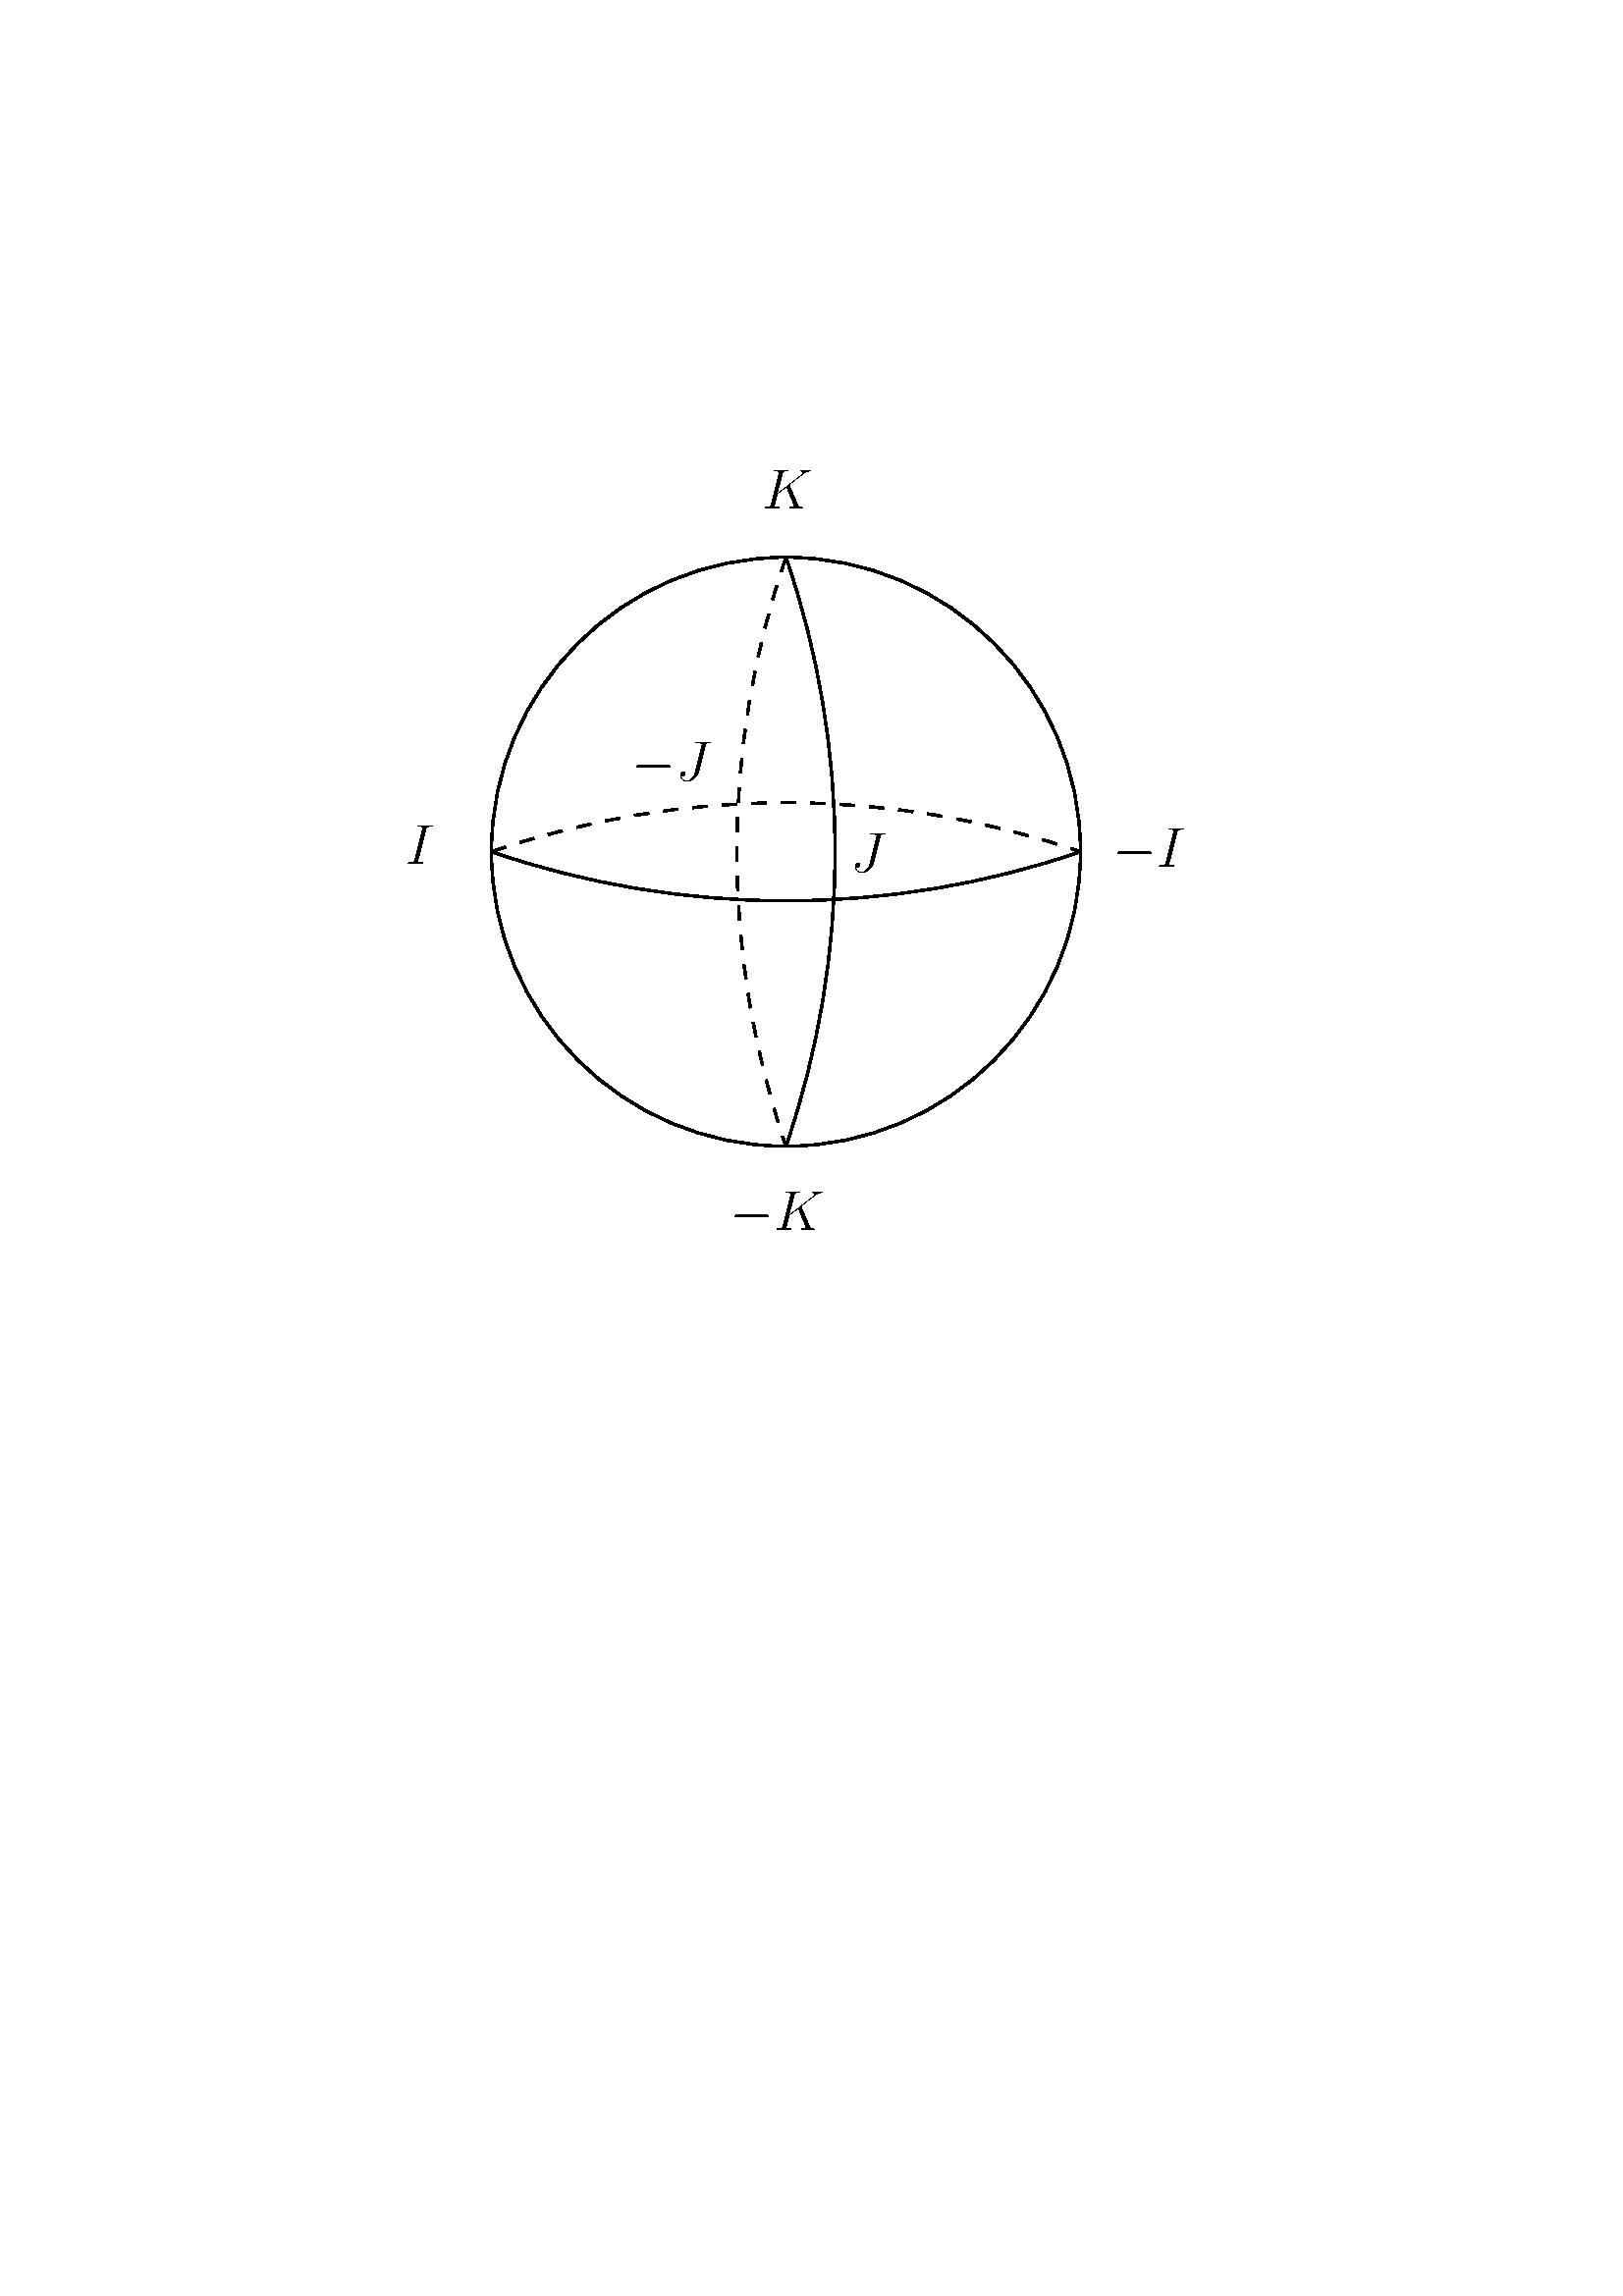
\includegraphics[width=0.75\linewidth]{figures/gla0-2.png}
\caption{ \medskip 超凯勒流形 $\M_H$ 上的一族复结构。（原文 Fig.~2）}
\label{fig:xunko}
\end{figure}
像 $I, J$ 或 $K$ 这样的复结构，通常定义为切空间上的线性变换，但我们改为写下作用在余切空间上的转置矩阵 $I^t$、$J^t$ 与 $K^t$。我们用下式定义 $I^t$% 式 (4.3)
\setcounter{equation}{2}
\begin{equation}\label{eq:uttu}
\begin{aligned} I^t(\delta A_{\bar z} )& =
i\delta A_{\bar z} \\ I^t(\delta \phi_{z}) & = i\delta \phi_{ z}
\\ I^t(\delta A_{ z}) & = -i\delta A_{ z} \\ I^t(\delta
\phi_{\bar z}) & = -i\delta \phi_{\bar z}, \\\end{aligned}
\end{equation}它们确实保证 $I^2=(I^t)^2=-1$。仿射空间 $\EUW$ 上的平移不变复结构也可以这样刻画：指明 $\EUW$ 上哪些线性函数是全纯的。对于复结构 $I$，线性全纯函数是 $A_{\bar z}$ 与 $\phi_z$（在 $C$ 上任意点取值）。

类似地，我们通过下式定义复结构 $J$：
% 式 (4.4)
\setcounter{equation}{3}
\begin{equation}\label{eq:buttu}
\begin{aligned}J^t(\delta A_{\bar z}) & = -\delta \phi_{\bar
z}\\ J^t(\delta A_z) & = -\delta \phi_z \\  J^t(\delta\phi_{\bar
z}) &  = \delta A_{\bar z} \\ J^t(\delta \phi_{ z}) & = \delta
A_z.\\\end{aligned}
\end{equation}
线性全纯函数是 $\CA_{\bar z}=A_{\bar z}+i\phi_{\bar z}$ 与 $\CA_z=A_{z}+i\phi_z$，或者更简洁地写成 $\CA=A+i\phi$。

最后，我们通过下式定义复结构 $K$：
% 式 (4.5)
\setcounter{equation}{4}
\begin{equation}\label{eq:bluttu}
\begin{aligned}K^t(\delta A_{\bar z} )& = -
i\delta\phi_{\bar z} \\ K^t(\delta \phi_{\bar z}) & = - i\delta
A_{\bar z} \\ K^t(\delta A_{ z} )& =  i\delta\phi_{ z} \\
K^t(\delta \phi_{ z}) & = i\delta A_{ z}. \\\end{aligned}
\end{equation}
线性全纯函数是 $A_{\bar z}-\phi_{\bar z}$ 与 $A_z+\phi_z$。

这些 $\EUW$ 余切空间上的线性变换满足 $I^tJ^t=-J^tI^t=-K^t$ 及其循环置换。取转置，我们就得到四元数关系的通常形式 $IJ=-JI=K$，等等。

除四元数关系之外，超凯勒结构的定义还要求度规 $ds^2$ 在每一个复结构下都是 $(1,1)$ 型。等价地，我们希望 $ds^2=I^t\otimes I^t(ds^2)=J^t\otimes J^t(ds^2)=K^t\otimes K^t(ds^2).$ 这一点可以直接验证。由于 $\EUW$ 是仿射空间且我们的复结构是线性的，没有别的东西需要检查；我们已经得到 $\EUW$ 上的一个平坦超凯勒结构。

一个超凯勒流形有（\xunko）由 $\Bbb{CP}^1$ 参数化的一族复结构，它们是 $I$、$J$ 与 $K$ 的线性组合。在我们所考虑的情形中，可以很简单地描述这族结构。对任意 $w\in \Bbb{C}^*$，我们考虑复结构 $I_w$，在其中 $A_{\bar z}-w\phi_{\bar z}$ 与 $A_z+w^{-1}\phi_z$ 全纯。于是 $w=-i$ 对应复结构 $J$，$w=1$ 对应 $K$。我们把定义延拓到包含 $w=0,\infty$：置 $I_0=I$，$I_\infty=-I$（这里 $-I$ 是与 $I$ 相反的复结构，其中 $A_z$ 与 $\phi_{\bar z}$ 全纯），因为它们是 $I_w$ 在 $w\to 0,\infty$ 时的极限。这样我们就得到所期望的那族复结构，它由一份 $\Bbb{CP}^1$ 参数化，我们把它记作 $\Bbb{CP}^1_h$（见 \zunko）。$I_w$ 的显式为
% 式 (4.6)
\setcounter{equation}{5}
\begin{equation}\label{eq:wyre}
I_w={1-\bar w w\over 1+\bar w w}I+{i(w-\bar w)\over
1+\bar w w}J+{w+\bar w\over 1+\bar w w}K.
\end{equation}
当然，它具有 $aI+bJ+cK$ 的形式，其中 $a^2+b^2+c^2=1$。

\providecommand{\CU}{{\cal U}}
我们引入一个群 $\CU_1\cong U(1)$，它按 $\phi_z\to \lambda\phi_z$、$\phi_{\bar z}\to \lambda^{-1}\phi_{\bar z}$（$|\lambda|=1$）作用于 $\phi$，同时保持 $A$ 固定。$\CU_1$ 保持超凯勒度规，并按下式作用于 $\Bbb{CP}^1_h$：% 式 (4.7)
\setcounter{equation}{6}
\begin{equation}\label{eq:zungo}
I_w\to I_{\lambda^{-1}w};
\end{equation}

它使两个点 $w=0,\infty$ 保持不动。我们在第~\ref{sec:complexstr}~节 末尾说明，$\CU_1$ 的作用在什么意义上延拓为其复化 $\CU\cong \Bbb{C}^*$ 的作用。

这族中 $\EUW$ 上的大多数复结构依赖于 $C$ 的复结构。例外的是 $J$——它可以刻画为使得 $\CA=A+i\phi$ 全纯的复结构——以及 $-J$，在其中 $\bar\CA=A-i\phi$ 全纯。$\EUW$ 上其余的复结构对 $A$ 与 $\phi$ 的 $z$ 分量与 $\bar z$ 分量区别对待，而这种区分依赖于 $C$ 的复结构。

对称群 ${\cal U}_1$ 是否来自四维杨--米尔斯理论的对称性？这个问题的答案稍微微妙。扭化的 ${\EUN}=4$ 超对称杨--米尔斯理论紧化到 $C$ 上后确实具有对称群 $\CU_1$。它通过旋转 $\phi_2-\phi_3$ 平面来作用；这是 $SU(4)_{\cal R}$ 的一个子群，在此特定紧化中未被破坏。然而，这并不给出底层那族四维拓扑场论的对称性，因为它不保持那族超对称生成元 $\epsilon=u\epsilon_\ell+v\epsilon_\rr$（它把这族生成元映到一个更大的族，我们在第~\ref{sec:twistedtft}~节 中讨论其解释，这些超对称缺少完整的 $Spin'(4)$ 对称性）。

但元素 $-1\in {\cal U}_1$ 确实来自四维拓扑场论的对称性。这个元素在 $\MH$ 上的作用，就像我们在第~\ref{sec:reviewsd}~节 中引入的中心元素 ${\EUI}\in SU(4)_{\cal R}$ 那样。事实上，${\EUI}$ 在 $SU(4)_{{\cal R}}$ 的 ${\bf 4}$ 中作用为 $i$，因此它在 ${\bf 6}=\wedge^2{\bf 4}$ 上作用为 $-1$，而后者正是包含 $\phi$ 的表示。（注意 ${\EUI}$ 也反转未扭化标量的符号。）变换 $\phi\to-\phi$ 在复结构 $I$ 下全纯，但在结构 $J$ 与 $K$ 下反全纯。这个变换的不动点集的显然分支由 $\phi=0$ 定义（正如我们后面讨论的，这给出稳定丛模空间 $\M$ 到 $\MH$ 的一个嵌入）。还有 \cite{ref20} 其他不动点集分支，在其中 $\phi$ 与 $-\phi$ 规范等价。

\par\medskip{\it 辛结构}

与 $\EUW$ 上超凯勒结构相联系的三个辛结构可定义为 $\omega_I = I^t\otimes 1(ds^2)$，类似地 $\omega_J=J^t\otimes 1(ds^2)$ 与 $\omega_K=K^t\otimes 1(ds^2)$。我们得到% 式 (4.8)
\setcounter{equation}{7}
\begin{equation}\label{eq:tomog}
\begin{aligned}\omega_I
& = -{i\over 2\pi}\int_C|d^2z|\,\Tr\left(\delta A_{\bar z}\wedge
\delta A_z-\delta \phi_{\bar z}\wedge \delta\phi_z\right)\\
&=-{1\over 4\pi}\int_C\,\Tr\left(\delta A\wedge \delta A
-\delta\phi\wedge\delta \phi\right) \\
                      \omega_J & ={1\over 2\pi}\int_C |d^2z|\,\Tr\left(
                      \delta\phi_{\bar z}\wedge \delta A_z+\delta\phi_z\wedge
                      \delta A_{\bar z} \right)\\
                      \omega_K & =
                      {i\over 2\pi}\int_C|d^2z|\,\Tr\left(\delta\phi_{\bar z}
                      \wedge\delta A_z-\delta\phi_z\wedge\delta A_{\bar z}\right)\\
                      & = {1\over 2\pi}\int_C \,\Tr\,\delta\phi
                      \wedge\delta A.\\\end{aligned}
\end{equation}

这里，$\omega_J$ 依赖于 $C$ 的复结构，而 $\omega_I$ 与 $\omega_K$ 不依赖。

此外，$\omega_I$ 关于复结构 $I$ 是 $(1,1)$ 型，$\omega_J$ 与 $\omega_K$ 也类似。我们还定义 $\Omega_I=\omega_J+i\omega_K$，以及循环置换 $\Omega_J=\omega_K+i\omega_I$、$\Omega_K=\omega_I+i\omega_J$：
 % 式 (4.9)
\setcounter{equation}{8}
\begin{equation}\label{eq:ninto}
\begin{aligned}\Omega_I & =
{1\over \pi}\int_C|d^2z|\,\Tr\,\delta\phi_z\wedge \delta A_{\bar
z} \\
        \Omega_J & =-{i\over 4\pi}\int_C\,\Tr\,\delta \CA\wedge\delta \CA          \\
        \Omega_K & = -{i\over 2\pi}\int_C |d^2z|\,\Tr\,\left( \delta A_{\bar z}\wedge
\delta A_z-\delta \phi_{\bar z}\wedge \delta\phi_z -
\delta\phi_{\bar z}\wedge \delta A_z-\delta\phi_z\wedge
                      \delta A_{\bar z}\right).\\\end{aligned}
\end{equation}

$\Omega_I$ 在复结构 $I$ 下是 $(2,0)$ 型，类似地 $\Omega_J$ 与 $\Omega_K$ 在各自的复结构下也是 $(2,0)$ 型。$\Omega_I$ 与 $\Omega_K$ 依赖于 $C$ 的复结构，但 $\Omega_J$ 不依赖。

闭二形式 $\omega_J$ 与 $\omega_K$ 实际上是恰当的。确实，我们可以非常显式地写出 $\omega_J=\delta\lambda_J$，其中 $\lambda_J={1\over 2\pi}\int_C |d^2z|\,\Tr\,\left(\phi_{\bar z}\delta A_z+\phi_z\delta A_{\bar z}\right)$。$\lambda_J$ 是规范不变的，因为 $\phi$ 与 $\delta A$（不同于 $A$ 本身）都在 $G$ 的伴随表示中变换。类似地 $\omega_K=\delta\lambda_K$，其中 $\lambda_K={1\over 2\pi}\int_C\,\Tr\,\phi\wedge \delta A$。除其他事项外，这意味着 $\MH$ 上的一个拓扑平凡线丛可以被赋予一个联络，其曲率是 $\omega_J$ 与 $\omega_K$ 的任意所需线性组合。只需把该联络取为 $\lambda_J$ 与 $\lambda_K$ 的适当线性组合即可。

另一方面，$\omega_I$ 在拓扑上非平凡。要按上面的方式写出 $\omega_I=\delta\lambda_I$，就需要在 $\lambda_I$ 中包含一个正比于 $\int \Tr \,A\wedge \delta A$ 的项，但由于 $A$ 在规范变换下的非齐次变换，这一项不是规范不变的。不过，我们可以写 $\omega_I=\omega_I'+\delta\lambda_I$，其中 $\lambda_I=(1/4\pi)\int_C\Tr\,\phi\wedge\delta\phi$，而
% 式 (4.10)
\setcounter{equation}{9}
\begin{equation}\label{eq:frox}
\omega_I'=-{1\over 4\pi}\int_C\Tr\,\delta A\wedge\delta
A.
\end{equation}
于是 $\omega_I$ 与 $\omega_I'$ 上同调，且特别地 $\omega_I$ 的上同调类是从 $\phi=0$ 的子空间拉回得到的。对单连通的 $G$，$\M$ 上线丛的 Picard 群是 $\Bbb{Z}$，由一个线丛 ${{\frak L}}$ 生成，其第一 Chern 类在 de Rham 上同调中由 $\omega_I'/2\pi$ 代表。我们会不严格地把 ${{\frak L}}$ 称作行列式线丛，因为对经典 $G$，它可以定义为 \cite{ref60} 一个 $\bar\partial$ 算子的行列式。\footnote{对 $G=SU(N)$，若 $E\to C$ 是秩为 $N$ 的全纯向量丛，则行列式线丛 $\frak L$ 在 $E$ 处的纤维 ${\frak L}_E$ 为 ${\frak L}_E=\det\,H^0(C,E)^{-1}\otimes \det\, H^1(C,E)$，其中 $\det\,V$ 表示向量空间 $V$ 的最高外幂。如此定义的线丛 $\frak L\to \M$ 是丰沛的。有些作者把我们称为 $\frak L$ 的东西写作 ${\frak L}^{-1}$。}

\par\medskip{\it Hitchin 模空间作为超凯勒商}

现在我们考虑按显然方式作用于 $\EUW$ 的规范变换群。它显然保持度规 \eqref{eq:igob}\ 与三个辛结构 \eqref{eq:tomog}。一个简短的计算表明，Hitchin 方程 \eqref{eq:zongo}\ 等价于对应于辛结构 \eqref{eq:tomog} 的三个 moment map 的消失。具体地说，设 $\epsilon$ 生成一个无穷小规范变换（因此 $\epsilon$ 是取值于 ${\rm ad}(E)$ 的零形式），并设 $V(\epsilon)$ 是 $\EUW$ 上相应的向量场，它按 $\delta A=-D\epsilon$、$\delta\phi=[\epsilon,\phi]$ 作用。那么辛结构 $\omega$ 的 moment map $\mu$ 通过解条件 $\iota_{V(\epsilon)}\omega=\delta\mu$ 得到（这里 $\iota_{V(\epsilon)}$ 是与 $V(\epsilon)$ 缩并的算子）。取 $\omega$ 为 $\omega_I$、$\omega_J$ 或 $\omega_K$，相应的 moment map 为
% 式 (4.11)
\setcounter{equation}{10}
\begin{equation}\label{eq:joget}
\begin{aligned}\mu_I & =-{1\over
2\pi}\int_C\,\Tr\,\epsilon(F-\phi\wedge \phi),\\ \mu_J &
=-{1\over 2\pi}\int_C|d^2z|\,\Tr\,\epsilon\left(D_z\phi_{\bar
z}+D_{\bar z}\phi_z\right), \\ \mu_K& = -{i\over
2\pi}\int_C|d^2z|\,\Tr\,\epsilon\left(D_z\phi_{\bar z}-D_{\bar
z}\phi_z\right).\\\end{aligned}
\end{equation}
一般地，若 $X$ 是一个超凯勒流形，李群 $H$ 以 moment map $\vec\mu=(\mu_I,\mu_J,\mu_K)$ 作用于其上，则方程 $\vec\mu=0$ 的解集对 $H$ 的商是超凯勒流形 \cite{ref61}，称为 $X$ 对 $H$ 的超凯勒商 $X/\negthinspace/\negthinspace/H$。因此特别地，$\M_H$ 是无穷维空间 ${\EUW}$ 对规范变换群的超凯勒商，并且是一个超凯勒流形。

可以给出一个更「物理」的解释，说明为什么 sigma 模型的靶空间是 $\EUW$ 的超凯勒商。一般地，在具有 $(4,4)$ 超对称与规范群 $H$ 的二维规范场论中，超多重态参数化一个超凯勒流形 $X$，而低能物理（为简单起见假设 $H$ 自由作用于 $X$）是一个 sigma 模型，其靶空间为超凯勒商 $X/\negthinspace/\negthinspace/H$。（超凯勒商构造最初正是在这一背景下被发现的 \cite{ref61}。）在目前的例子中，把四维扭化拓扑规范场论紧化到二维，得到的就是一个具有 $(4,4)$ 超对称的理论。（扭化与紧化保留了原来十六个超对称中的八个，其中四个具有一种二维手征性，另外四个具有另一种。）这个二维理论的规范群是 $C$ 到 $G$ 的映射构成的群 ${\cal G}$，而超多重态参数化 $\EUW$。这正是导致 $\MH$ 作为超凯勒商出现的那套设定。所以低能物理是一个 sigma 模型，其靶空间为 $\EUW$ 的超凯勒商。

\par\medskip{\it 维数约化的更精确描述}

我们现在可以更精确地讨论从扭化四维超对称杨--米尔斯理论到靶空间为 $\MH$ 的 sigma 模型的维数约化。这样的 sigma 模型有一个度规与一个 $B$-场。我们想确定它们是什么。

我们考虑 $M=\Sigma\times C$ 上的四维超对称杨--米尔斯理论，其中 $\Sigma $ 的半径远大于 $C$ 的半径。规范场的动能是
% 式 (4.12)
\setcounter{equation}{11}
\begin{equation}\label{eq:kinen}
{{\cmmib I}}_{kin}=-{1\over 2e^2}\int_{\Sigma\times C}
|d^2y|\,|d^2z|\,\Tr\,F_{\mu\nu}F^{\mu\nu},
\end{equation}
其中 $|d^2y|$ 与 $|d^2z|$ 分别是 $\Sigma$ 与 $C$ 上的黎曼测度。这个表达式有 $(p,q)$ 型的贡献（$p+q=2$），其中 $p$ 是切于 $\Sigma$ 的指标 $\mu,\,\nu$ 的个数，$q$ 是切于 $C$ 的个数。把 $\Sigma\times C$ 上的规范场写成 $A=A_\Sigma+A_C$ 是有用的，其中 $A_\Sigma$ 切于 $\Sigma$，$A_C$ 切于 $C$。

$(0,2)$ 型的项是 $A_C$ 的势能的一部分，它使理论局域在缓变映射 $\Phi:\Sigma\to \MH$ 上。$(2,0)$ 型的项给出 $A_\Sigma$ 的动能；在 $\MH$ 的奇点之外，由于规范群被完全破坏，这些场是有质量的，可以在红外区被积掉（正如我们在第~\ref{sec:wilbranes}~节 中明确描述的）。

sigma 模型的动能来自 $(1,1)$ 型的项。这些项是% 式 (4.13)
\setcounter{equation}{12}
\begin{equation}\label{eq:binen}
-{1\over e^2}\int
|d^2y|\,|d^2z|\,\sum_{\mu=0,1}\sum_{\nu=2,3}\,\Tr\,F_{\mu\nu}F^{\mu\nu}.
\end{equation}

我们想把它与映射 $\Phi:\Sigma\to X$ 的一般 sigma 模型相比较，其中靶空间 $X$ 用局部坐标 $X^I$ 写成度规 $ds^2_X=g_{IJ}(X)\,dX^I\,dX^J$。于是 sigma 模型的动能为
% 式 (4.14)
\setcounter{equation}{13}
\begin{equation}\label{eq:zinen}
\int |d^2y|\, g_{IJ}\sum_{\mu=0,1}\partial_\mu
X^I\partial^\mu X^J.
\end{equation}
在比较 \eqref{eq:binen}\ 与 \eqref{eq:zinen}\ 时，$X^I$ 的角色由 $A_C$ 扮演，而 $F_{ij}$ 对应于 $\partial_i X^I$。如果把 \eqref{eq:binen}\ 与 \eqref{eq:zinen}\ 和我们对 ${\EUW}$ 上超凯勒度规 $ds^2$ 的原始定义 \eqref{eq:igob}\ 相比较（该度规在超凯勒商 $\MH$ 上诱导出一个我们也称为 $ds^2$ 的度规），就会看到由四维规范场论诱导的度规 $ds^2_g$ 与 $ds^2$ 的关系为% 式 (4.15)
\setcounter{equation}{14}
\begin{equation}\label{eq:inog}
ds^2_g={4\pi\over e^2}\,ds^2=({\rm
Im}\,\tau)\,ds^2.
\end{equation}

类似地，我们想约化规范场论的 $\theta$ 项，它在欧氏号差下为% 式 (4.16)
\setcounter{equation}{15}
\begin{equation}\label{eq:bloko}
{\cmmib
I}_\theta={i\theta\over 8\pi^2}\int_{\Sigma\times C}\,\Tr\,
F\wedge F.
\end{equation}
同样地，我们对代表到 $\MH$ 的缓变映射的规范场来赋值这个耦合。由于 ${{\cmmib I}}_\theta$ 的拓扑不变性，在计算 \eqref{eq:bloko}\ 时我们可以形变到 $F$ 在 $C$ 上的限制为零的情形（即 $F_{23}=0$）。形变到 $F|_C=0$ 可以通过一个复规范变换或利用 Hitchin 的第二纤维化 $\MH\to\M$ 来实现（这两个概念我们后面都会解释）。既然如此，在计算 ${\cmmib I}_\theta$ 时，我们可以把 $F={1\over 2}\sum_{\mu,\nu=0}^3dx^\mu\wedge dx^\nu \,F_{\mu\nu}$ 替换为 $F^{1,1}=\sum_{\mu=0,1}\sum_{\nu=2,3}dx^\mu\wedge dx^\nu \,F_{\mu\nu}$。在 sigma 模型极限下，$F^{1,1}$ 对应于 $\delta A_C=\sum_{\mu=0,1}dx^\mu \,D_\mu A_C$，而 ${\cmmib I}_\theta$ 约化为\footnote{出现一个负号是因为：在定义 $\omega_I'$ 时，$\delta$——即联络 $A_C$ 构成的空间上的外微分——被取为与 $C$ 上诸如 $dx^ j$（$j=2,3$）这样不依赖于 $A_C$ 的一形式交换。而对于 $\Sigma\times C$ 上的微分形式（${\cmmib I}_\theta$ 正是用它定义的），它们会反交换。}
% 式 (4.17)
\setcounter{equation}{16}
\begin{equation}\label{eq:ino}
-{i\theta\over 8\pi^2}\int_\Sigma \int_C \Tr\,\delta
A_C\wedge \delta A_C.
\end{equation}

与 $\omega_I'$ 的定义 \eqref{eq:frox}\ 相比较，我们看到这等价于% 式 (4.18)
\setcounter{equation}{17}
\begin{equation}\label{eq:zinok}
{i\theta\over
2\pi}\int_\Sigma\Phi^*(\omega'_{I})={i\theta\over 2\pi}\int_\Sigma
\Phi^*(\omega_I),
\end{equation}
其中最后一步用到了 $\omega_{I}-\omega'_{I}$ 是恰当的这一事实。在一般 sigma 模型中，$B$-场是靶空间 $X$ 上的闭二形式；它通过一项 $-i\int_\Sigma\,\Phi^*(B)$ 出现在作用量中。因此，有效低能 sigma 模型的 $B$-场为
% 式 (4.19)
\setcounter{equation}{18}
\begin{equation}\label{eq:palooka}
B=-{\theta\over 2\pi}\omega_I=-({\rm
Re}\,\tau)\,\omega_I.
\end{equation}

我们可以更概念化地描述这一点。对单连通的 $G$，瞬子数 $(1/8\pi^2)\int_M \Tr\,F\wedge F$ 对任意四维流形 $M$ 都取整数值。此外，对单连通的 $G$，$\MH$ 是单连通的，因而 $H^2(\MH,\Bbb{Z})=\pi_2(\MH)$。形式 $\omega_I$ 的归一化使得 $\omega_I/2\pi$ 是 $H^2(\MH,\Bbb{Z})$ 的一个生成元在 de Rham 上同调中的像。这些事实意味着：对任意 $\Sigma$ 与 $C$，存在映射 $\Phi:\Sigma\to \MH$ 使 $\int_\Sigma\Phi^*(\omega_I/2\pi)=1$（而且这是可达到的最小值）。这样的映射对应于 $M=\Sigma\times C$ 上一个规范场，其瞬子数按约定为 $\pm 1$。\footnote{在物理论文中，四维瞬子一般取为自对偶规范场，满足 $F^-=0$；而在数学文献中，一般取为反自对偶，满足 $F^+=0$。如果把 sigma 模型中的瞬子理解为到 $\MH$ 的全纯映射，并采用四维中通常的物理约定，那么瞬子数为 1 的 sigma 模型场来自瞬子数为 $-1$ 的规范场论瞬子。通常的数学约定避免了这一负号。}更简单地说，二维与四维中的 $\theta$ 角相同，因为瞬子是相同的。若 $G$ 不是单连通的，情况会稍复杂一些；瞬子数不总是整数，而在 sigma 模型一侧也有相应的复杂化。

\begin{yizhu}[易错点]
按：$I$ 与 $J$ 的区分是本节乃至整个 §4 的枢纽，务必记牢。复结构 $I$ 中的线性全纯函数是 $A_{\bar z}$ 与 $\phi_z$：这把 $A$ 的 $(0,1)$ 部分读作全纯丛的结构、把 $\phi$ 的 $(1,0)$ 部分读作 Higgs 场，于是 $I$ 对应「半稳定 Higgs 丛」的图像；复结构 $J$ 中的全纯函数是 $\CA=A+i\phi$，即复平坦联络，于是 $J$ 对应「平坦 $G_{\Bbb C}$ 丛」的图像（记作 $Y$，而且 $J$ 不依赖 $C$ 的复结构）；$K=IJ$ 是第三个结构。相应地把参数对应关系记住：$w=-i\leftrightarrow J$，$w=1\leftrightarrow K$，$w=0\leftrightarrow I$，$w=\infty\leftrightarrow -I$。后面讨论 $S$-对偶时交换的是 $I$ 与 $J$（A-模型与 B-模型的靶空间互换），若把这两个复结构弄混，膜与 Hitchin 纤维的对应就会全部颠倒。
\end{yizhu}

\begin{yizhu}[易错点]
按：(4.11) 的三个 moment map 方程 $\mu_I=\mu_J=\mu_K=0$ 就是 Hitchin 方程。具体地，$\mu_I=0$ 给出 $F-\phi\wedge\phi=0$；而 $\mu_J=0$ 与 $\mu_K=0$ 合起来等价于两个复方程 $D_z\phi_{\bar z}=0$ 与 $D_{\bar z}\phi_z=0$——取 $\mu_J$ 与 $\mu_K$ 的线性组合时，对称部分与反对称部分分别消去一个方向。这正是四维中 $D\phi=0$、$D\star\phi=0$ 两个实方程在二维的化身。另一个易混点是量纲：$\EUW$ 是无穷维仿射空间，$\epsilon$ 取值在 ${\rm ad}(E)$ 中，moment map 作为 $\EUW$ 上的「函数」其实取值在对偶空间（即分布）里，所以 (4.11) 中保留了 $\int_C\Tr\,\epsilon(\dots)$ 的积分形式；不要以为这是多余的记号。
\end{yizhu}

\begin{yizhu}[物理图像]
按：这一段是超凯勒商构造的原始物理背景。二维 $(4,4)$ 超对称规范理论中，超多重态的参数空间是超凯勒流形 $X$，规范群 $H$ 的作用给出超凯勒商 $X/\negthinspace/\negthinspace/H$：低能下超多重态被约束到 moment map 零点，而规范多重态有质量、被积掉。在本例中 $X=\EUW$（无穷维！）、$H={\cal G}={\rm Maps}(C,G)$，所以 $\MH=\EUW/\negthinspace/\negthinspace/{\cal G}$ 自动继承超凯勒结构。无穷维的商之所以能给出有限维流形，是因为 Hitchin 方程是椭圆方程组，其解模空间有限维；这一「无穷维商仍超凯勒」的机制正是后面所有超凯勒几何论证的基础。
\end{yizhu}

\begin{yizhu}[含糊点拨]
按：(4.15) 与 (4.19) 合起来说明二维 sigma 模型的两个连续参数恰好来自四维的规范耦合：度规由 $e^2$ 决定、$B$-场由 $\theta$ 决定。若取本书的复耦合约定 $\tau=\theta/2\pi+4\pi i/e^2$，则 ${\rm Im}\,\tau=4\pi/e^2$ 给出度规、${\rm Re}\,\tau=\theta/2\pi$ 给出 $B$-场，二者合起来正是 $\tau$。注意 $B$-场正比于 $\omega_I$（而不是 $\omega_J$ 或 $\omega_K$）：因为 $\theta$ 项的约化只留下 $\omega_I'$ 的部分，而 $\omega_I$ 与 $\omega_I'$ 上同调，故在作用量中可以互换。$B$-场不是四维理论的基本数据，而是 $\theta$ 项在紧化下的产物；话虽如此，它在二维理论中却是能灵敏感知瞬子数的数据。
\end{yizhu}

\begin{yizhu}[易错点]
按：为什么二维 sigma 模型的 $\theta$ 角与四维规范理论的 $\theta$ 角相同？关键在于 $\int_\Sigma\Phi^*(\omega_I/2\pi)=1$ 与四维瞬子数是同一个拓扑量：$\omega_I/2\pi$ 是 $H^2(\MH,\Bbb{Z})$ 生成元的 de Rham 像，故它在二维的积分是整数；而这个整数正是四维第二 Chern 数（瞬子数）在约化下的像，所以两边用同一个 $\theta$ 加权。末段脚注提醒物理与数学文献对自对偶/反自对偶的约定差一个符号，故同一个位形在两边瞬子数标号相反（$\pm 1$）；这是约定问题，并非方程不一致。
\end{yizhu}

\begin{yizhu}[含糊点拨]
按：$\omega_J,\omega_K$ 恰当而 $\omega_I$ 不恰当，这个不对称是 Hitchin 模空间几何的核心之一。$\omega_I$ 的上同调类来自 $\phi=0$ 的子空间（即稳定丛模空间 $\M$）的拉回，并由行列式线丛 $\frak L$ 的第一 Chern 类代表；$\omega_J,\omega_K$ 的恰当性则让 $\MH$ 上存在曲率为任意线性组合的联络。脚注中的行列式线丛在经典群时可用 $\bar\partial$ 算子的行列式定义，其丰沛性（ample）与稳定性及嵌入有关。另：本片用到的 harvmac 遗留宏不要展开或改名——\xunko 展开为「fig.~2」、\zunko 展开为「fig.~1」（是原文图号，不是 \verb|\ref{fig:...}|，勿替换）；$\CU$ 在此处是群 $\CU_1\cong U(1)$ 及其复化 $\CU\cong \Bbb{C}^*$，与别处把 $\CU$ 用作 Bun$_G$ 的记号不同，注意区分。
\end{yizhu}

%% ============================================================
%% 分片 10：原文第 4 节「Compactification And The Geometry Of Hitchin's Moduli Space」（原文 glshort.tex 起于第 2325 行）
%% 由 tools/harvmac2tex.py 从 arXiv 源码（hep-th/0604151v3）自动生成。
%% 只译英文散文；公式、编号、\label、\cite 一律不改。
%% ============================================================

\subsection{$\MH$ 的复结构}

\label{sec:complexstr}

我们下一步的任务是更具体地理解 $\MH$ 上的复结构。

\par\medskip\emph{用全纯数据描述}

让我们从复结构 $I$ 的角度来考察 $\EUW$ 的超凯勒商。组合
$\nu_I=\mu_J+i\mu_K$ 在这个复结构下是全纯的：
% 式 (4.20)
\setcounter{equation}{19}
\begin{equation}\label{eq:uttup}
\nu_I=-{1\over \pi}\int_C|d^2z|\,\Tr\,\epsilon\,D_{\bar
z}\phi_z.
\end{equation}
 $\nu_I$ 在复结构 $I$ 下全纯，因为它是从 $\Omega_I$ 导出的 moment map，而
后者在复结构 $I$ 下是 $(2,0)$ 型的（具体地说，$\nu_I$ 之所以全纯，是因为它只依赖于 $A_{\bar z}$ 与 $\phi_z$）。
在这类问题中，把全纯 moment map $\nu_I$ 的零点与实 moment map $\mu_I$ 的零点分开考虑，往往是很方便的 \cite{ref61}。

黎曼面 $C$ 上光滑 $G$-丛 $E$ 上的任何联络 $A$ 都自动把 $E$ 变成全纯 $G$-丛
（我们仍用同一个名字记它，但愿这不会引起混淆）。只需把 $\bar\partial$ 算子定义为
$\bar D=d\bar z\,D_{\bar z}$；在复维数为一的情形，它平凡地满足 $\bar D^2=0$。全纯
moment map $\nu_I$ 为零告诉我们 $\bar D\phi=0$；换言之，
$\varphi=\phi_z\,dz$ 是 $K_C\otimes {\rm
ad}(E)$ 的一个全纯截面，其中 $K_C$ 是 $C$ 的典范线丛。
换个说法，$\varphi$ 是一个取值于伴随表示、也就是取值于 $E$ 的伴随丛的全纯
1-形式。我们把由 $G$-丛 $E$ 与 $K_C\otimes {\rm ad}(E)$ 的全纯截面 $\varphi$ 组成的
对 $(E,\varphi)$ 称为 Hitchin 对。$\varphi$ 常被称为 Higgs 场，而赋以 $\varphi$
之选择的丛 $E$ 也称为 Higgs 丛。

要得到模空间 $\MH$，我们还必须把实 moment map $\mu_I$ 置零，并模去取值于 $G$ 的
规范变换所构成的群。然而，正如 \cite{ref20} 所利用的（这也是模问题中常有的情形），
理解这些合在一起的步骤有一个更简单的办法。全纯 moment map $\nu_I$ 的零点空间 $\EUW_0$
不仅容许通常取值于 $G$ 的规范变换作用，还容许取值于 $G$ 的复化 $G_{\Bbb{C}}$ 的
规范变换作用。这一点从 $\nu_I$ 的全纯性看得很清楚。于是我们可以对 $\EUW_0$
施行以下两种操作之一：

\emph{(I)} 限制到 $\EUW_0$ 中满足 $\mu_I=0$ 的子空间，再模去取值于 $G$ 的规范变换。

\emph{(II)} 用取值于 $G_{\Bbb{C}}$ 的规范变换去除 $\EUW_0$。

操作 \emph{(I)} 给出所要的模空间
$\MH$，但操作 \emph{(II)} 容易理解得多，且与它几乎重合。
（两者几乎重合的原因是：几乎每条复规范变换轨道都包含唯一一条满足 $\mu_I=0$ 的通常规范变换轨道。）
理解操作 \emph{(I)} 最容易的办法，常常是先理解操作 \emph{(II)}，再理解它与操作 \emph{(I)} 的关系。

在当前的例子中，操作 \emph{(II)} 的结果很容易描述。它的意思是：我们不关心 $A_{\bar z}, $ $\phi_z$ 的具体取法，
而只关心由 $A_{\bar z}$ 决定的全纯 $G$-丛 $E$，以及与之相关联的
$K_C\otimes {\ad}(E)$ 的全纯截面 $\varphi$。
因此，在当前的例子中，操作 \emph{(II)} 给出的是 Hitchin 对 $(E,\varphi)$ 的等价类的集合。

这个集合在许多用途上都是 $\MH$ 的极好近似；
例如当 $C$ 的亏格至少为 2 时，两者只相差余维相当高的集合。更准确地说（本文大部分
内容并不依赖于这些细节），我们需要稳定性这一概念。
对 $G=SU(2)$，我们把 $E$ 解释为 $C$ 上秩为二的复全纯向量丛，把 $\varphi$ 解释为全纯映射 $\varphi:E\to E\otimes K_C$。
若一个线丛 ${\cal L}\subset E$ 满足 $\varphi({\cal L})\subset {\cal L}\otimes K_C$，则称它
为 $\varphi$-不变的。若每个 $\varphi$-不变的线丛 ${\cal L}\subset E$ 的第一 Chern 类都是负的，则称
Hitchin 对 $(E,\varphi)$ 为稳定的。若每个这样的 ${\cal L}$ 的第一 Chern 类都非正，则称它
为半稳定的。对一般的 $G$，必须考虑把 $E$ 的结构群约化到 $G_{\Bbb{C}}$ 的极大抛物子群 $P$ 的 $\varphi$-不变约化。带这种约化的丛 $E$ 有一个自然的第一 Chern 类
（因为 $P$ 带有一个特殊的 $U(1)$）；若对每个这样的约化，第一 Chern 类都是负的（或非正的），则称对
$(E,\varphi)$ 为稳定（或半稳定）的。半稳定但不稳定的对称为严格半稳定的。

稳定性是一个温和的条件，意思是：例如若
$(E,\varphi)$ 是稳定的，则每个邻近的对也是稳定的。此外，不稳定的对具有很高的余维（如果 $C$ 的亏格大于 1）。

现在我们可以回到比较操作 \emph{(I)} 与 \emph{(II)} 的问题，或者等价地说，回到用全纯语言描述 Hitchin 方程解的模空间 $\MH$ 的问题。
\cite{ref20} 证明的结果是：$\MH$ 等同于「稳定对 $(E,\varphi)$ 的模空间」，即稳定 Hitchin 对。要得到这个模空间，我们扔掉不稳定的 Hitchin 对，对半稳定的那些施加某种等价关系，然后模去复值规范变换。这个对操作 \emph{(II)} 稍作修改的版本——称之为操作 \emph{(II)$'$}——与操作 \emph{(I)} 恰好一致。

总之，$\MH$ 参数化稳定的 Hitchin 对 $(E,\varphi)$，以及严格半稳定 Hitchin 对的某些等价类。稳定对对应于 $\MH$ 中的光滑点，也对应于（对某些 $G$）某些轨形奇点（orbifold 奇点）。严格半稳定的对一般会导致 $\MH$ 中比轨形奇点更糟糕的奇点。

\par\medskip\emph{复结构 $J$ 的类比}

以上这些在复结构 $J$ 中都有类比。复结构 $J$ 中的全纯 moment map 是 $\nu_J=\mu_K+i\mu_I$：
% 式 (4.21)
\setcounter{equation}{20}
\begin{equation}\label{eq:nuJ}
\nu_J =-{i\over 2\pi}\int_C\,\Tr\,\epsilon{\cal F}
\end{equation}
 为
构造 $\MH$，我们首先要求 $\nu_J$ 为零。$\nu_J$ 的一个零点不过是一对 $A,\phi$，使得曲率
${\cal F}$（属于取值于 $G_{\Bbb{C}}$ 的联络 $\CA=A+i\phi$）等于零。因此，如果我们用取值于 $G_{\Bbb{C}}$ 的
规范变换群去除 $\nu_J$ 的零点集，就恰好得到全部同态 $\vartheta:\pi_1(C)\to G_{\Bbb{C}}$ 在共轭下的集合 ${\cal Y}_0$。这就是操作 \emph{(II)}。

相反，要得到 $\MH$，我们应当施行操作 \emph{(I)}。换句话说，我们应当置 $\mu_J=0$，即施加条件 $D^*\phi=0$，并且只模去取值于 $G$ 的规范变换。
与复结构 $I$ 的情形一样，在比较这两种操作时，稳定性这一概念会介入。
对 $G=SU(2)$，若同态 $\vartheta:\pi_1(C)\to G_{\Bbb{C}}$ 的单值不能同时化归为三角形式 % 式 (4.22)
\setcounter{equation}{21}
\begin{equation}\label{eq:yto}
\left(\begin{matrix} \alpha &
\beta \\ 0 & \alpha^{-1}\end{matrix}\right).
\end{equation}
   则称该同态为稳定的。若 $\vartheta$ 有这样的化归，则称它为严格半稳定的。（在复结构
$J$ 中，没有不稳定表示的概念。）若两个严格半稳定表示具有相同的对角单值元素，即相同的 $\alpha$，则认为它们等价。
注意每个这样的等价类都含一个 $\beta=0$ 的特殊代表元。

对任何 $G$，把单值放进三角形式的类比，是把它们共轭进 $G$ 的一个抛物子群 $P$ 中。若一个表示不能被这样共轭，则称它为稳定的，
否则称为严格半稳定的。严格半稳定表示上的等价关系对任何 $G$ 都有自然的类比
（两个都约化到 $P$ 的严格半稳定表示等价，如果这两个平坦 $P$-丛投影到 $P$ 的极大约化子群后变得等价）。

Corlette \cite{ref58} 与 Donaldson 的一个定理（见 \cite{ref20} 的附录）说：$\MH$ 在复结构 $J$ 中就是
参数化稳定同态 $\vartheta:\pi_1(C)\to G_{\Bbb{C}}$ 以及半稳定同态之等价类的模空间 ${{\cal Y}}$。

\par\medskip\emph{$I_w$ 的类比}

我们刚才所说的，在每个复结构 $I_w$（$w\not= 0,\infty$）中都有直接的类比。复结构 $I_w$ 中的全纯
变量是 $A_{\bar z}-w\phi_{\bar z}$、$A_z+w^{-1}\phi_z$。
Hitchin 方程中的两个方程合起来给出全纯条件 $[D_{\bar z}-w\phi_{\bar
z},D_z+w^{-1}\phi_z]=0$，第三个是一个 moment map 条件。
该全纯条件说明：分量为 $(A_{\bar z}-w\phi_{\bar z},A_z+w^{-1}\phi_z)$ 的复值联络是平坦的。
把 moment map 置零并模去规范变换，得到的模空间与我们在复结构 $J$ 中找到的 ${{\cal Y}}$ 相同。
因此所有复结构 $I_w$（$w\not=0,\infty$）都是等价的。

事实上，在复结构 $I=I_{w=0}$ 中，我们可以定义一个对称群 ${\cal U}\cong \Bbb{C}^*$，它作用在
Higgs 丛上为 $(E,\varphi)\to (E,\lambda\varphi)$，
$\lambda\in\Bbb{C}^*$。（稳定性条件在这个变换下不变。）当 $|\lambda|=1$ 时，它约化为第~\ref{sec:mhhyper}~节中描述的群
${\cal U}_1$，后者是 $\MH$ 的超凯勒度量的一个对称群。当 $|\lambda|\not=1$ 时，
我们得不到 $\MH$ 的超凯勒度量的对称，但正如 \cite{ref20} 第 107-8 页所示，
我们得到 $\MH$ 的一个微分同胚群，它保持复结构 $I$，并通过 % 式 (4.23)
\setcounter{equation}{22}
\begin{equation}\label{eq:trymodo}
I_w\to
I_{\lambda^{-1}w},
\end{equation}
 变换其他复结构，从而把式 \eqref{eq:zungo}\ 推广到
$|\lambda|\not=1$。

\subsection{Hitchin 纤维化}

\label{sec:hitchfib}

现在我们来更详细地讨论 $\MH$ 的几何。

若 $E$ 是稳定的 $G$-丛，则对 $(E,0)$ 是稳定的
Hitchin 对。于是我们得到 $C$ 上稳定 $G$-丛的模空间 $\M$ 到 Hitchin 模空间
$\MH$ 的自然嵌入。在复结构 $I$ 中，$\M$ 是 $\MH$ 的全纯子流形，因为它由方程
$\phi_z=0$ 定义，而这些方程在复结构 $I$ 中全纯。在复结构
$J$ 与 $K$ 中，$\M$ 不是全纯的。相反，它是 Lagrangian 的，因为 $\phi=0$ 蕴含 $\delta\phi=0$，从而
$\mu_J=\mu_K=0$。

若 $E$ 是稳定的，则对每个 $\varphi\in H^0(C,K_C\otimes\ad(E))$，Hitchin 对 $(E,\varphi)$ 都是稳定的。此外，${\EUM}$ 在点 $E$ 处的
切丛是 $H^1(C,\ad(E))$（它参数化 $E$ 的一阶形变），故由 Serre
对偶，$\M$ 在点 $E$ 处的余切空间是
$H^0(C,K_C\otimes\ad(E))$。于是 $\varphi$ 取遍这个
余切空间中的值，而所有满足 $E$ 稳定的 $(E,\varphi)$ 构成的空间就是余切丛
$T^*\M$。因此我们实际上得到
$T^*\M$ 到 $\MH$ 的嵌入。$\MH$ 在复结构 $I$ 中的全纯辛形式
$\Omega_I$ 限制到 $T^*\M$ 上，正好是它作为全纯余切丛的自然辛结构
（也就是说，对 $\M$ 上任意的局部全纯坐标 $q^\alpha$
，存在在 $T^*\M\to \M$ 的纤维上线性的全纯函数 $p_\alpha$，使得
$\Omega_I=\sum_\alpha dp_\alpha\wedge dq^\alpha$）。\footnote{这个断言成立，是因为类似
的断言在取超凯勒商之前的全部对 $(A,\phi)$ 构成的空间 $\EUW$ 上实际上成立。$\EUW$
可以理解为联络空间 ${\EUA}$ 的余切空间，$A$ 参数化 ${\EUA}$，而 $\phi$
参数化 ${\EUA}$ 的余切空间；$\Omega_I$ 就是 ${\EUW}$ 看作
$T^*{\EUA}$ 时的自然全纯辛形式。一般来说，这种类型的结构在取复辛商
（在现下的情形中，即置 $\nu_I=0$ 并模去取值于 $G_{\Bbb{C}}$ 的规范变换）时保留下来。}

$T^*\M$ 在 $\MH$ 中的像并不是整个 $\MH$，因为 Hitchin 对 $(E,\varphi)$ 可能在 $E$ 不稳定时仍然稳定。
然而，那些 $E$ 不稳定的稳定 Hitchin 对 $(E,\varphi)$ 构成一个余维非常高的集合。扔掉
这个集合后，$\MH$ 同构于 $T^*\M$，并且有一个通过忘掉 $\varphi$ 而得到的到
$\M$ 的自然映射。尽管这个映射只在去掉一个余维非常高的集合之后才有定义，它却
极其有用。我们称它为 Hitchin 的第二纤维化（第一个纤维化是我们马上就要引入的另一个映射）。

\par\medskip\emph{Hitchin 纤维化}

在复结构 $I$ 中，除了把 $\varphi$ 映为零之外，另一个自然的操作
是计算 $\varphi$ 的规范不变多项式。对 $G=SU(2)$，这简单意味着我们考虑
二次 Casimir 算子 $w=\Tr\,\varphi^2$。由于
$\bar D\varphi=0$，我们有 $\bar\partial w=0$，所以 $w$ 是一个全纯二次微分，取值于
${\EUBB}=H^0(C,K_C^2)\cong \Bbb{C}^{3g-3}$。最常被称为 Hitchin 纤维化的映射，是把对 $(E,\varphi)$ 映到
$w=\Tr\,\varphi^2$ 所得的映射 $\pi:\MH\to {\EUBB}$。

对任何 $G$，Hitchin 纤维化的定义类似，只是人们用 $\varphi$ 的全部独立
Casimir（即全部独立的 $G$-不变多项式）来刻画 $\varphi$，而不只是二次的那个。例如
对 $G=SU(N)$，我们定义 $w_n=\Tr\,\varphi^n$
（$n=2,\dots,N$），并令 ${\EUBB}=\oplus_{n=2}^NH^0(C,K_C^n)$。
于是 Hitchin 纤维化就是把 $(E,\varphi)$ 映到点 $(w_2,w_3,\dots,w_n)\in {\EUBB}$ 的映射。对任何 $G$，人们考虑
的则是代替 $\Tr\,\varphi^n$ 的适当独立齐次 $G$-不变多项式 ${\cal P}_i$。这些多项式的个数
等于 $G$ 的秩 $r$，它们的次数 $d_i$ 满足恒等式 % 式 (4.24)
\setcounter{equation}{23}
\begin{equation}\label{eq:yty}
\sum_{i=1}^r(2d_i-1)={\rm
dim}(G).
\end{equation}
 例如对 $G=SU(N)$，$d_i$ 是 $2,3,\dots,N$，
于是 $\sum_i(2d_i-1)=N^2-1={\rm dim}(G)$。最后，一般地我们定义 ${\EUBB}=\oplus_i H^0(C,K_C^{d_i})$。

由于 $\dim \,H^0(C,K_C^n)=(2n-1)(g-1)$，由 \eqref{eq:yty}\
可知 ${\EUBB}$ 的复维数是 $(g-1){\rm dim}(G)$，
它等于 $\M$ 的维数，也等于
$\M_H$ 维数的一半。Hitchin 纤维化 $\pi:\MH\to {\EUBB}$ 是满射，这一点我们马上就会讨论。由于 Hitchin 纤维化的底空间
${\EUBB}$（即映射 $\pi:\MH\to {\EUBB}$ 的靶空间）的维数是 $\MH$ 维数的一半，可知 $\pi$ 的一般纤维 $\CMF$ 的维数也是 $\MH$ 维数的一半，
从而等于 ${\EUBB}$ 的维数：
% 式 (4.25)
\setcounter{equation}{24}
\begin{equation}\label{eq:yrof}
\dim\,\CMF=\dim\,{\EUBB}={1\over
2}\dim\,\MH=(g-1)\dim\,G.
\end{equation}

让我们定性地解释为什么 Hitchin 纤维化是满射。例如取 $G=SU(2)$。取一个稳定的 $SU(2)$
丛 $E$。考虑方程 $\Tr\,\varphi^2=w$，其中
$\varphi $ 在 $(3g-3)$ 维空间
$H^0(C,K_C\otimes \ad(E))$ 中变化，而 $w$ 是
$(3g-3)$ 维空间 ${\EUBB}=H^0(C,K_C^2)$ 中的固定元素。这是
$3g-3$ 个复变量的 $3g-3$ 个二次方程组成的方程组。
解的一般个数是 $2^{3g-3}$。对其他 $G$ 也可以作类似的计数。

\par\medskip\emph{完全可积性}

\cite{ref62}

 我们现在想解释 Hitchin 的一个主要结果 ：$\MH$ 在复结构 $I$ 中是一个完全可积的哈密顿系统。我们可以找到 ${1\over 2}{\rm
dim}\MH$ 个 $\MH$ 上的函数 $H_a$，它们在复结构
$I$ 中全纯、代数无关，并且关于由全纯辛形式 $\Omega_I$ 得到的 Poisson 括号两两
Poisson 交换。\footnote{读者可能不习惯这种全纯意义上的完全可积系统。
从这样的系统可以提取通常实意义上的完全可积哈密顿系统（而且有趣且重要的构造正以这种方式出现；例子见
\cite{ref63,ref64}）。我们选取 $C$ 使它能容许一个实结构——即一个反转其复结构的对合。这在 $\M$ 与 $\MH$ 上诱导出实结构。
通过特殊化到 $\MH$ 中的一个实切片，就得到完全可积的哈密顿系统，其中相空间坐标、辛结构与交换的哈密顿量全都是实的。}

事实上，我们可以取 $H_a$ 为 ${\EUBB}$ 上的线性函数，因为 ${\EUBB}$ 的维数恰好等于所需的函数个数。
我们先对 $G=SU(2)$ 解释这一构造。首先取 $(3g-3)$ 维空间 $ H^1(C,T_C)$ 的一组基 $\alpha_a$
（$a=1,\dots,3g-3$），该空间与 $H^0(C, K_C^2)\cong {\EUBB}$ 对偶。（这里 $T_C$ 是
$C$ 的全纯切丛。）我们把 $\alpha_a$ 用取值于 $T_C$ 的 $(0,1)$-形式表示，并仍用同一个名字称呼它们，
然后定义 % 式 (4.26)
\setcounter{equation}{25}
\begin{equation}\label{eq:miro}
H_a=\int_C\alpha_a \wedge \Tr\,\varphi^2.
\end{equation}
 我们断言，这些函数关于全纯辛形式 $\Omega_I$ 两两 Poisson 交换。

一个自然的证明利用了下述事实：$H_a$ 的定义在取超凯勒商之前、在无穷维空间 $\EUW$ 上就有意义。
用 $\EUW$ 上的辛结构 $\Omega_I$ 来定义 Poisson 括号，$H_a$ 显然两两 Poisson 交换。因为在这些 Poisson 括号下（给定 $\Omega_I$ 的形式 \eqref{eq:ninto}\ ），$\varphi_z$ 与 $A_{\bar z}$ 共轭，
而与自身交换。但 $H_a$ 只是 $\varphi_z$ 的函数，不是 $A_{\bar z}$ 的函数。

这些函数 $H_a$ 可以限制到 $\nu_I=0$ 的轨迹上，
又因为它们在取值于 $G_{\Bbb{C}}$ 的规范变换下不变，它们下降到 $\MH$ 上的全纯函数。辛约化
的一个一般性质是：它把 Poisson 交换的函数映为 Poisson 交换的函数
（辛约化即把某个 moment map——这里是 $\nu_I$——置零，再模去相应的群——这里是取值于 $G_{\Bbb{C}}$ 的规范变换群）。
所以 $H_a$ 作为 $\MH$ 上的函数两两 Poisson 交换。它们的个数足够多，足以建立 $\MH$ 的完全可积性。

这个构造中有一点需要注意：作为 $\EUW$ 上的函数，$H_a$
依赖于代表上同调类的、取值于 $T$ 的 $(0,1)$-形式 $\alpha_a$ 的具体选取。
任何选取都可以，但我们必须作出选择。然而在限制并下降到 $\MH$ 之后，我们在 $\MH$ 上得到的函数只依赖于 $\alpha_a$ 的上同调类。事实上，一旦有 $\bar D\varphi=0$，从而
$\bar\partial\Tr\,\varphi^2=0$，$H_a$ 显然在
$\alpha_a\to\alpha_a+\bar\partial\epsilon_a$ 下不变。

Poisson 交换的函数 $H_a$ 在
$\MH$ 上生成彼此交换的流，这些流在复结构 $I$ 中全纯。
复环面容许交换的流，人们可能会猜测由 $H_a$ 生成的轨道至少一般地是复环面。这一点
由关于全纯辛结构与 Hitchin 纤维化的纤维紧性的普遍结果推出，也可以更直接地证明，即使用
谱覆盖技术 \cite{ref20,ref62}。这项技术在本课题的进一步发展中有
许多应用，将在别处解释 \cite{ref26}。在本文中，我们将在不使用谱覆盖构造的前提下尽量推进。

对任何 $G$，上述构造的类比是把 $\Tr\,\varphi^2$ 换成一个次数为 $d_i$ 的一般规范不变多项式 ${\cal
P}_i$。相应的交换哈密顿量取形式 $H_{\alpha,i}=\int_C \alpha \,{\cal P}_i(\varphi)$，其中
$\alpha\in H^1(C,K_C^{1-d_i})$。利用维数公式 \eqref{eq:yty} 作一个简单的维数计数即可说明，这些哈密顿量
在数目上恰好足以建立 $\MH$ 的完全可积性。利用 Hitchin 纤维化的纤维是紧的（从而全纯函数必是该纤维化底空间上的拉回）这一事实，可以证明这些交换哈密顿量生成
$\MH$ 上的全纯函数环。

完全可积性的一个简单而重要的推论是：Hitchin 纤维化的纤维是
$\Omega_I$ 这一全纯辛结构中的 Lagrangian 子流形，等价地也是实辛结构 $\omega_J$ 与
$\omega_K$ 中的 Lagrangian 子流形。事实上，该纤维化的一条纤维由方程 $H_k-h_k=0$ 定义，其中 $H_k$ 是交换的哈密顿量
而 $h_k$ 是复常数。一般来说，一组中间维数的 Poisson 交换函数（如
现下的 $H_k-h_k$）的零点集是 Lagrangian 的。

\begin{yizhu}[易错点]
稳定性的方向容易记反：对 $G=SU(2)$，稳定要求每个 $\varphi$-不变线丛 ${\cal L}\subset E$ 的第一 Chern 类为负（半稳定则要求非正）。这里的「负」是就 ${\cal L}$ 的第一 Chern 数即次数而言，不是就某个斜率的大小而言。对一般 $G$，要看的对象变成 $E$ 到极大抛物子群 $P$ 的 $\varphi$-不变约化，其第一 Chern 类由 $P$ 中那个特殊的 $U(1)$ 给出。
\end{yizhu}

\begin{yizhu}[含糊点拨]
为什么操作 (II) 与操作 (I) 几乎重合？原文只说「几乎每条复规范变换轨道都包含唯一一条满足 $\mu_I=0$ 的通常规范变换轨道」。按：这是 Kempf-Ness 型的论断——复群 $G_{\Bbb{C}}$ 的轨道与 $\mu_I^{-1}(0)$ 的交在稳定点处是单个 $G$-轨道，只有严格半稳定的轨道才会出现多解，所以本小节末尾要额外加上「半稳定对之间的等价关系」这一层。
\end{yizhu}

\begin{yizhu}[物理图像]
$T^*\M\hookrightarrow\MH$ 给出了 Hitchin 模空间的直观图像：在复结构 $I$ 下，$\MH$ 在余维很高的坏集之外就是稳定 $G$-丛模空间 $\M$ 的余切丛，而 Higgs 场 $\varphi$ 正是余切方向上的坐标。按：这正是几何 Langlands 把「$G$-丛上的 Hecke 修正」与「$\MH$ 中膜的形变」联系起来的几何基础（参见 Witten 2008 综述第 2 节）。
\end{yizhu}

\begin{yizhu}[原文疑误]
本片倒数第四个自然段中「取值于 $T$ 的 $(0,1)$-形式 $\alpha_a$」里的 $T$，按前文应读作 $T_C$（$C$ 的全纯切丛）；注意到 $\alpha_a$ 是 $H^1(C,T_C)$ 中元素的代表，原文此处显系笔误，译文照录。
\end{yizhu}

\begin{yizhu}[易错点]
$w=\Tr\,\varphi^2$ 不是函数而是二次微分，它取值于 $K_C^2$，所以 Hitchin 底空间是 ${\EUBB}=H^0(C,K_C^2)$ 而不是某个函数空间。对 $SU(2)$ 有 $\dim {\EUBB}=3g-3=\dim\M=\frac12\dim\MH$；这个「维数正好是一半」的事实正是后面纤维维数公式 (4.25) 的来源，也是完全可积性所需的函数个数。
\end{yizhu}

\begin{yizhu}[含糊点拨]
完全可积性的证明是「先在无穷维空间算、再下降到模空间」的典型：$H_a$ 定义在超凯勒商之前的 $\EUW$ 上，在那里 $\Omega_I$ 使 $\varphi_z$ 与 $A_{\bar z}$ 共轭，而 $H_a$ 只含 $\varphi_z$，故 Poisson 交换是显然的；再由辛约化把 Poisson 交换性带到 $\MH$。按：这也是原文不必写出具体括号计算的原因——真正的内容是「辛约化保持 Poisson 交换性」这一普遍性质。
\end{yizhu}

%% ============================================================
%% 分片 11：原文第 5 节「Topological Field Theory In Two Dimensions」（原文 glshort.tex 起于第 3264 行）
%% 由 tools/harvmac2tex.py 从 arXiv 源码（hep-th/0604151v3）自动生成。
%% 只译英文散文；公式、编号、\label、\cite 一律不改。
%% ============================================================

\section{二维拓扑场论}
\label{sec:tqfttwo}

\begin{keytakeaways}
  \begin{itemize}[leftmargin=1.4em,itemsep=2pt,topsep=2pt]
    \item \textbf{物理图像}：把第~\ref{sec:tqftfour}~节得到的四维扭化规范理论放到 $M=\Sigma\times C$ 上紧化（$C$ 是一张黎曼面），低能有效理论就是以 Hitchin 模空间 $\MH$ 为靶空间的二维拓扑 sigma 模型；$\MH$ 的超凯勒结构使它自动具有 $(4,4)$ 超对称。
    \item \textbf{数学工具}：四维扭化参数族 $\Bbb{CP}^1_g$ 与二维 $(2,2)$ 超对称所需的复结构对 $(J_+,J_-)$（即 $\Bbb{CP}^1_h\times\Bbb{CP}^1_h$ 中的一点）可以对齐，嵌入由 $w_+=-t$、$w_-=t^{-1}$ 给出，这里 $t$ 是四维扭化参数。
    \item \textbf{关键结论}：四维 $S$-对偶在二维表现为镜像对称——它交换 $A$-模型与 $B$-模型，从而把几何 Langlands 纲领表述为 Hitchin 模空间上膜范畴之间的等价。
    \item \textbf{边界与展望}：当 $J_-\ne\pm J_+$ 时所得模型既非 $A$-模型也非 $B$-模型，需要广义复几何才能把它约化为 $A$-模型；这正是本节后半与后续各节的出发点。
  \end{itemize}
\end{keytakeaways}

在第~\ref{sec:tqftfour}~节中，我们分析了 ${\cal N}=4$ 超对称杨-米尔斯理论在一个一般四维流形 $M$ 上的一个扭化版本。扭化保留了那些在子群 $Spin'(4)\subset Spin(4)\times Spin(6)$ 下不变的超对称。一个超对称生成元在 $Spin'(4)$ 下不变的条件是
% 式 (5.1)
\setcounter{equation}{0}
\begin{equation}\label{eq:tory}
\left(\Gamma_{\mu\nu}+\Gamma_{4+\mu,4+\nu}\right)\epsilon=0,
~~\mu,\nu=0,\dots,3.
\end{equation}
  此外，全部 16 个超对称生成元还满足一个十维手征条件，
% 式 (5.2)
\setcounter{equation}{1}
\begin{equation}\label{eq:nory}
\Gamma_0\Gamma_1\dots\Gamma_9\epsilon=\begin{cases}\epsilon&
~\text{in Lorentz signature}\\-i\epsilon&~\text{in Euclidean
signature.}\\\end{cases}
\end{equation}
 在扭化理论中，${\EUN}=4$ 超对称杨-米尔斯理论的六个标量场 $\phi_0,\dots,\phi_5$ 当中有四个被重新解释为一个 1-形式 $\phi=\sum_{\mu=0}^3\phi_\mu\,dx^\mu$。两个标量场 $\phi_4$ 与 $\phi_5$ 没有被扭化，它们在一个群 $SO(2)_{\cal R}$（我们在第~\ref{sec:twisting}~节中把它的生成元记作 ${\cal K}$）下转动。把费米子也一并计入，扭化理论的对称群是 $Spin(2)_{\cal R}$，即 $SO(2)_{\cal R}$ 的双重覆盖。

扭化理论是一种形式上的构造，因为扭化破坏酉性，并且只在欧几里得号差下才成立。\footnote{要在 Lorentz 号差下构造扭化理论，我们需要一个合适的同态 $Spin(1,3)\to Spin(6)$。由于 $Spin(6)$ 是紧的，这样的非平凡同态并不存在。若改把 $Spin(6)$ 换成 $Spin(1,5)$ 来绕开这一困难，则与费米子的耦合就不再是厄米的，能量也不再下有界。}然而，假定我们把时间方向分离出来，取 $M=\Bbb{R}\times W$，其中 $\Bbb{R}$ 参数化时间，$W$ 是一个三维流形，并且 $M$ 上的度量为乘积度量。那么时间不参与扭化，扭化理论在 Lorentz 号差或欧几里得号差下都说得通，并且是酉的、物理上合理的。此时 $M$ 的和乐群（holonomy group）约化为 $SO(3)$，未破缺的超对称只需在子群 $Spin'(3)\subset Spin'(4)$ 下不变；等价地说，我们只需对 $\mu,\nu=1,\dots,3$ 施加 \eqref{eq:tory}。共有四个未破缺的超对称生成元，它们对 $\mu,\nu=1,\dots 3$ 满足 \eqref{eq:tory}。有三个标量没有被扭化，即 $\phi_0$、$\phi_4$ 与 $\phi_5$，它们在一个 $Spin(3)_{\cal R}$ 对称下转动，该对称扩充了任何 $M$ 上都存在的 $Spin(2)_{\cal R}$ 对称。

让我们进一步特殊化到 $M=\Bbb{R}^{1,1}\times C$（或 $\Bbb{R}^2\times C$）的情形，其中 $C$ 是一张黎曼面。$M$ 的和乐群约化为 $SO(2)$，而 \eqref{eq:tory} 归结为单个条件
\begin{equation*}
\tag*{(5.3)}
\Gamma_{2367}\epsilon=\epsilon,\label{eq:ytytag}
\end{equation*}
留下一个八维的未破缺超对称空间。四个标量 $\phi_0,\phi_1,\phi_4$ 与 $\phi_5$ 没有被扭化，而转动未扭化标量的对称群此时扩充为 $Spin(4)_{\cal R}$。

事实上，二维中的结构恰好就是 $(4,4)$ 超对称的结构。若把 \eqref{eq:ytytag} 与 \eqref{eq:nory} 结合起来，我们得到（在 Lorentz 号差下）% 式 (5.4)
\setcounter{equation}{3}
\begin{equation}\label{eq:byty}
\Gamma_{01}\epsilon
=\Gamma_{4589}\epsilon.
\end{equation}
 这里 $\Gamma_{01}$ 是区分 $\Bbb{R}^{1,1}$ 的 Lorentz 群 $SO(1,1)$ 的两个旋量表示的算子。类似地，$\Gamma_{4589}$ 区分 $Spin(4)_{\cal R}=SU(2)'\times SU(2)''$ 的两个旋量表示。这两个旋量表示在 $SU(2)'\times SU(2)''$ 下分别按 $({\bf 2},{\bf 1})$ 与 $({\bf 1},{\bf 2})$ 变换。式 \eqref{eq:byty} 说明：对所有的二维超对称，$\Gamma_{01}$ 与 $\Gamma_{4589}$ 的本征值都相等。

于是，在适当选取 $\Bbb{R}^{1,1}$ 的定向之后，超对称按 $({\bf 2},{\bf 1})^-\oplus({\bf 1},{\bf 2})^+$ 变换，其中上标标记 $\Gamma_{01}$ 的本征值。但这正是二维中 $(4,4)$ 超对称的通常结构：一个 $SU(2)$ 的 $R$-对称群——即 $SU(2)'$——作用在负 $Spin(1,1)$ 手征的超对称上，而第二个这样的群——$SU(2)''$——作用在正手征的超对称上。事实上，在第~\ref{sec:compacthitchin}~节中，我们已经把低能有效理论确定为靶空间是超凯勒流形 $\MH$ 的 sigma 模型。一般来说，靶空间为超凯勒流形的 sigma 模型具有 $(4,4)$ 超对称 \cite{ref65}。

除了 $Spin(4)_{\cal R}$ 整体对称之外，$\Bbb{R}^{1,1}\times C$ 上的扭化规范理论还有一个额外对称，它之所以出现，是因为我们据以扭化的 $C$ 的和乐群是阿贝尔的。即使在扭化 $\phi_2$ 与 $\phi_3$ 之后，仍然可以对 $\phi_2-\phi_3$ 平面作转动。这就是第~\ref{sec:mhhyper}~节中称为 ${\cal U}_1$ 的对称群，它作用在 Hitchin 对 $(E,\varphi)$ 上，把 $\varphi$ 的相位转动。

\begin{yizhu}[原文疑误]
此处原文说的是把式 (5.3) 与式 (5.2) 结合起来。harvmac 源码里 $\Gamma_{2367}\epsilon=\epsilon$ 这个词条被写成了无编号的 \texttt{tag*} 公式（源文件用同名宏 \verb|\yty| 定义了两次，第二次即 (5.3)），译本已为它补上标签 \texttt{eq:ytytag}，故 \eqref{eq:ytytag} 正确指向 (5.3)。按：这是排版脚手架问题，不是原文笔误。
\end{yizhu}

\begin{yizhu}[易错点]
扭化只在欧几里得号差下成立：它破坏酉性（脚注给出了理由——紧群 $Spin(6)$ 与非紧的 $Spin(1,3)$ 之间不存在非平凡同态）。但一旦把时间方向分离出来写成 $M=\Bbb{R}\times W$，扭化就与时间无关，理论在 Lorentz 号差下也可以既酉又物理。读本文时不要因为第一句话就把扭化理论当作纯形式的玩具。
\end{yizhu}

\begin{yizhu}[含糊点拨]
注意未被扭化的标量数目随流形而变：一般四维流形 $M$ 上为 2 个（$\phi_4,\phi_5$），$\Bbb{R}\times W$ 上为 3 个（$\phi_0,\phi_4,\phi_5$），$\Bbb{R}^{1,1}\times C$ 上为 4 个（$\phi_0,\phi_1,\phi_4,\phi_5$）；相应地 $R$-对称从 $Spin(2)_{\cal R}$ 逐步扩充为 $Spin(3)_{\cal R}$、$Spin(4)_{\cal R}$。按：这些数目正是二维 $(4,4)$ 超对称中每个「4」的来源。
\end{yizhu}

\begin{yizhu}[物理图像]
$\Gamma_{01}\epsilon=\Gamma_{4589}\epsilon$ 把两件不同的事绑在一起：$\Gamma_{01}$ 标记 $\Bbb{R}^{1,1}$ 上 $SO(1,1)$ 的两种手征，$\Gamma_{4589}$ 标记 $R$-对称群 $SU(2)'\times SU(2)''$ 的两个二重态。二者本征值相等，意味着二维的手征与 $R$-对称的 $SU(2)$ 标记同步，这正是二维 $(4,4)$ 超对称的标准结构；也正因为如此，靶空间为超凯勒流形的 sigma 模型才「自动」是 $(4,4)$ 的。
\end{yizhu}

\begin{yizhu}[含糊点拨]
本节最后一段的 ${\cal U}_1$ 对称值得留意：它之所以存在，是因为用来扭化的 $C$ 的和乐群 $SO(2)$ 是阿贝尔的——扭化用掉了 $\phi_2,\phi_3$ 所在的二维平面，但该平面内仍可整体转动。这个 ${\cal U}_1$ 与复结构 $I_w$ 族上的 $\Bbb{C}^*$ 作用（第~\ref{sec:complexstr}~节末）是同一件事在 $|\lambda|=1$ 时的限制，后面讨论 T-对偶与镜像对称时还会用到。
\end{yizhu}

%% ============================================================
%% 分片 12：原文第 5 节「Topological Field Theory In Two Dimensions」（原文 glshort.tex 起于第 3264 行）
%% 由 tools/harvmac2tex.py 从 arXiv 源码（hep-th/0604151v3）自动生成。
%% 只译英文散文；公式、编号、\label、\cite 一律不改。
%% ============================================================

\subsection{扭化拓扑场论}

\label{sec:twistedtft}

我们现在想从拓扑场论的观点来研究靶空间为 $\MH$ 的 sigma 模型，因此把
$\Bbb{R}^{1,1}$ 换成一个一般的二维流形 $\Sigma$，最终我们将取它带有欧几里得号差。我们想
讨论：由靶空间为 $\MH$ 的 sigma 模型可以构造出 $\Sigma$ 上的哪些扭化拓扑场论，以及其中哪些实际上来自把我们在第~\ref{sec:tqftfour}~节中
构造的四维拓扑场论在黎曼面 $C$ 上紧化。

 \cite{ref66}
 \cite{ref67}
\cite{ref68}


为了由靶空间为 $X$ 的 sigma 模型构造拓扑场论，人们在 $X$ 上取一\emph{对}满足 $(2,2)$ 超对称某些条件的
复结构 $(J_+,J_-)$ 。\footnote{广义复几何给出这一构造的一个推广，我们这里不需要它：在推广中，由对 $(J_+,J_-)$ 可以形成的两个广义复结构中 \cite{ref67}\ 只有一个可积。
然后人们像  那样，试图用这个可积的广义复结构来定义拓扑场论。}这些
条件最近被重新解释 ，所用语言是广义复几何 \cite{ref69}。一旦有了 $(2,2)$ 超对称，就有一个
标准配方 \cite{ref70}（通过我们在第~\ref{sec:twisting}~节中回顾过的扭化程序）来构造拓扑
场论。

若 $X$ 是超凯勒的，事情会简化。靶空间为 $X$ 的
sigma 模型具有 $(4,4)$ 超对称，而 $(2,2)$ 超对称的结构可以通过取
$(4,4)$ 超对称代数的一个 $(2,2)$ 子代数得到。\footnote{相差 $Spin(4)_{\cal R}$ 共轭的两个 $(2,2)$ 子代数
视为等价的。}就复结构的选择而言，这相当于以下内容。$X$ 有一族由一份
$\Bbb{CP}^1$ 参数化的复结构，我们把它记作
$\Bbb{CP}^1_h$；而取一对点 $(J_+,J_-)\in \Bbb{CP}_h^1$ 就可以定义一个 $(2,2)$ 结构。\cite{ref66}\ 中的条件对这样一对点
自动满足。对 $\MH$ 而言，这就给出对几何 Langlands 纲领重要的那族
拓扑场论。

我们可以如下方便地刻画与对 $(J_+,J_-)$ 相联的拓扑场论。设 $\Phi: \Sigma\to
\MH$ 是 sigma 模型的玻色场。那么未破缺超对称的方程为
% 式 (5.5)
\setcounter{equation}{4}
\begin{equation}\label{eq:hson}
(1-iJ_+)\bar\partial\Phi=0,
\end{equation}
 以及
% 式 (5.6)
\setcounter{equation}{5}
\begin{equation}\label{eq:hsono}
(1-iJ_-)\partial \Phi=0.
\end{equation}
  这里 $\partial$ 与
$\bar\partial$ 是 $\Sigma$ 上外微分的通常 $(1,0)$ 与 $(0,1)$ 部分；而 $\partial\Phi$ 与
$\bar\partial \Phi$ 理解为 $\Sigma$ 上取值于切丛 $TX$ 的拉回（$J_+$
与 $J_-$ 作用在其上）的 1-形式。第一个条件说映射
$\Phi:\Sigma\to X$ 在复结构 $J_+$ 中全纯；第二个说它在复结构 $J_-$ 中反全纯。
与我们在第~\ref{sec:familya}~节中找出未破缺超对称条件的方式类似，这些方程之所以出现，是因为存在费米场 $\chi_+$、$\chi_-$，使得
$\{Q,\chi_+\}=(1-iJ_+)\bar\partial\Phi$、
$\{Q,\chi_-\}=(1-iJ_-)\partial\Phi$。

方程 \eqref{eq:hson}\ 与 \eqref{eq:hsono}\ 中的信息远多于其解中的信息。为了讨论
方程的解，人们通常特殊化到欧几里得号差的 $\Sigma$（对拓扑场论来说这是最自然的情形）。
此时对一般的 $J_+$、$J_-$，它们蕴含映射
$\Phi:\Sigma\to X$ 必须是常值映射，而这个结果并不依赖于
$J_+$ 与 $J_-$。方程本身若从代数上理解、并且不固定二维流形
$\Sigma$ 上的实结构，则依赖于 $J_+$ 与 $J_-$。

一个重要的例子是 $J_+=J_-=\hat J$ 的情形（在我们的应用中，$\hat J$ 将是 $\MH$ 的复结构 $I_w$
之一，如式 \eqref{eq:wyre} 所述）。这些方程合起来给出
$(1-i\hat J\,)d\Phi = 0$，从而蕴含 $d\Phi=0$。该模型
称为复结构 $\hat J$ 中的 $B$-模型。反之若
$J_+=-J_-=\hat J$，我们就得到复结构 $\hat J$ 中的 $A$-模型。（这个模型实际上依赖于与复结构 $\hat J$ 相联的辛形式
$\omega_{\hat J}$，而不是复结构本身。但有时把「复结构 $\hat J$ 中的 $A$-模型」当作方便的简称。）对欧几里得号差的 $\Sigma$，
$A$-模型的方程是多余的，因为式 \eqref{eq:hsono}\ 是 \eqref{eq:hson}\ 的复共轭。
其中任何一个都断言映射 $\Phi:\Sigma\to \MH$ 在复结构 $\hat
J$ 中全纯。若 $J_-\not= \pm J_+$，我们得到的模型既不是
$A$-模型也不是 $B$-模型，但可以用广义复几何把它约化为 $A$-模型，正如我们在第~\ref{sec:gencpx}~节中讨论的那样。

我们回顾式 \eqref{eq:wyre}\ 中由 $\Bbb{CP}_h^1$ 参数化的 $\MH$ 上复结构族的显式形式。用
$\Bbb{CP}_h^1$ 的仿射参数 $w$ 来说，我们定义了一个复结构 $I_w$，其全纯坐标是
$A_{\bar z}-w\phi_{\bar z}$ 与 $A_z+w^{-1}\phi_z$。具体地，我们
得到 % 式 (5.7)
\setcounter{equation}{6}
\begin{equation}\label{eq:wyrre}
I_w={1-\bar w w\over 1+\bar w w}I+{i(w-\bar
w)\over 1+\bar w w}J+{w+\bar w\over 1+\bar w w}K.
\end{equation}

 在这个参数化下，对
$(J_+,J_-)$ 对应于对
$(w_+,w_-)$。

\par\medskip\emph{从四维约化}

现在让我们把它与从四维约化所得的结果作比较。我们在第~\ref{sec:tqftfour}~节中了解到，规范理论
给出定义在任何四维流形 $M$ 上、并由一份我们记作
$\Bbb{CP}^1_g$ 的 $\Bbb{CP}^1$ 参数化的一族拓扑量子场论（TQFT）。
这一族对 $M=\Sigma\times C$ 当然约化为族
$\Bbb{CP}_h^1\times \Bbb{CP}_h^1$ 中从二维观点看自然的子族。两族都来自对
四维流形 $M$ 上 ${\EUN}=4$ 超对称杨-米尔斯理论施行扭化程序。在该程序中，拓扑场论
由适当选取的超对称线性组合 $Q$ 的上同调得到。要得到族 $\Bbb{CP}^1_g$，我们
要求 $Q$ 是 $Spin'(4)$-不变的，以便构造对所有的 $M$ 都有效。但要得到靶空间为 $\MH$ 的 sigma 模型，我们
特殊化到约化和乐流形 $M=\Sigma\times C$，此时如我们后面更明确讨论的，对 $Q$ 的较弱条件就够了，从而得到更大的族 $\Bbb{CP}_h^1\times
\Bbb{CP}_h^1$。

我们希望把四维拓扑场论族 $\Bbb{CP}^1_g$ 辨认作 sigma 模型族
$\Bbb{CP}_h^1\times \Bbb{CP}_h^1$ 的子族。$\Bbb{CP}^1_g$
到 $\Bbb{CP}_h^1\times \Bbb{CP}_h^1$ 的嵌入可以用函数
$w_+(t)$、$w_-(t)$ 描述。通过特殊化到一个方便的构型或物理态，我们可以算出这些函数。

一个非常方便的做法是干脆把问题阿贝尔化，即在一个由某些未扭化标量场的
期望值把 $G$ 破缺到其极大环面的真空中工作。在阿贝尔情形，由 \eqref{eq:loopme}，四维中未破缺超对称的方程为
% 式 (5.8)
\setcounter{equation}{7}
\begin{equation}\label{eq:onso}
\begin{aligned}(F+t\,d\phi)^+&=0\\
(F-t^{-1}d\phi)^-&=0.\\
\end{aligned}
\end{equation}

这里，1-形式 $\phi$ 是 $T^*M=T^*\Sigma\oplus
T^*C$ 的截面，而规范场 $A$ 局部地是一个 1-形式或 $T^*M$ 的截面。为了与 $\Sigma$ 上靶空间为
$\MH(G,C)$ 的 sigma 模型比较，我们必须取 $\Sigma $ 的半径远大于
$C$ 的半径。在该极限下，$A$ 与 $\phi$ 中取值于
$T^*\Sigma$ 的部分是「有质量的」，可以丢掉；于是
$A$ 与 $\phi$ 可以解释为 $T^*C$ 的截面，在 $\Sigma$ 上缓慢
变化。

我们用 $y$ 记 $\Sigma$ 上的局部复坐标，用 $z$
记 $C$ 上的局部复坐标。2-形式 $d\bar
y\wedge d\bar z$ 是自对偶的，而 $dy\wedge d\bar z$ 是
反自对偶的。因此 \eqref{eq:onso} 中的第一个方程给出
% 式 (5.9)
\setcounter{equation}{8}
\begin{equation}\label{eq:igot}
\partial_{\bar y}\left(A_{\bar z}+t \phi_{\bar
z}\right)=0,
\end{equation}
 而第二个方程给出
% 式 (5.10)
\setcounter{equation}{9}
\begin{equation}\label{eq:nigot}
\partial_y\left(A_{\bar z}-t^{-1}\phi_{\bar
z}\right)=0.
\end{equation}

把这些结果与式 \eqref{eq:hson}\ 和 \eqref{eq:hsono}\ 比较，就可以读出函数 $w_+(t)$ 与 $w_-(t)$。式 \eqref{eq:igot}\ 断言：
若在 $\MH(G,C)$ 上取使 $A_{\bar z}+t\phi_{\bar
z}$ 全纯的复结构，则映射 $\Sigma\to \MH(G,C)$ 全纯。这与式 \eqref{eq:hson} 一致；后者断言
在复结构 $I_{w_+}$ 中全纯，当且仅当
$w_+=-t$。类似地，式 \eqref{eq:nigot}\ 断言映射 $\Sigma\to
\MH(G,C)$ 反全纯，如果我们在 $\MH(G,C)$ 上取使 $A_{\bar z}-t^{-1} \phi_{\bar z}$
全纯的复结构。这与式 \eqref{eq:hsono} 一致；后者断言在复结构 $I_{w_-}$ 中
反全纯，当且仅当
$w_-=t^{-1}$。

于是 $\Bbb{CP}^1_g$ 到 $\Bbb{CP}_h^1\times
\Bbb{CP}_h^1$ 的嵌入由 % 式 (5.11)
\setcounter{equation}{10}
\begin{equation}\label{eq:tyroy}
\begin{aligned}w_+ & = -t\\
                                              w_- & = t^{-1}.\\
\end{aligned}
\end{equation}
定义。

\par\medskip\emph{一些简单的考虑}

现在让我们对这个结果作几点简单的观察。

首先，我们什么时候得到 $B$-模型？对 $B$-模型，我们
要求 $w_+=w_-$。所以条件是 $t^{-1}=-t$，它恰好出现在
$t=\pm i$ 时。由于 $w=\mp i$ 时的复结构 $I_w$ 与 $J$、$-J$ 重合，这样我们就得到
复结构 $J$ 或 $-J$ 中的 $B$-模型。

我们什么时候得到 $A$-模型？对 $A$-模型，复结构
$I_{w_+}$ 与 $I_{w_-}$ 应当相反。映射
$w\to -1/\bar w$ 把 $I_w$ 映到它的相反结构（这从
\eqref{eq:wyrre} 看得很清楚），所以若 $w_-=-1/\bar
w_+$，我们就得到二维的 $A$-模型，这归结为 $t=\bar t$。换句话说，恰对实的 $t$，我们得到 $A$-模型。
例如对 $t=1$ 或
$-1$，我们得到复结构 $K$ 或 $-K$ 中的 $A$-模型。对
$t=0$ 或 $\infty$，我们得到复结构 $I$
或 $-I$ 中的 $ A$-模型。

现在，让我们把这个族与 sigma 模型更完整的族
$\Bbb{CP}_h^1\times \Bbb{CP}_h^1$ 作比较。在第~\ref{sec:complexstr}~节末尾，我们描述了 $\MH(G,C)$ 的微分同胚群 ${\cal U}\cong
\Bbb{C}^*$；它作用在复结构族 $I_w$ 上为 $w\to \lambda^{-1} w$，$\lambda\in
\Bbb{C}^*$。由对\footnote{这个拓扑场论还依赖于 $\MH$ 的超凯勒度量与 $B$-场。
对全部变量的完整依赖关系将在第~\ref{sec:gencpx}~节中用广义复几何确定。}
$(w_+,w_-)$ 确定的拓扑场论与由 $(\lambda^{-1} w_+,\lambda^{-1} w_-)$ 确定的相同。从二维观点看，我们能定义多少种真正不等价的 TQFT？
由对 $(w_+,w_-)$ 能构成的唯一不变量是比值 $q=w_+/w_-$。我们看到
\begin{equation*}
\tag*{(5.12)}
q=-t^2,
\end{equation*}
 所以 $q$ 的所有值都可以实现，但并非完全唯一。$\Bbb{CP}^1_g$ 上的点 $t$ 与 $-t $ 导致二维中相互等价的理论。这一等价
反映了 $SU(4)_{\cal R}$ 的中心的作用（回忆式
\eqref{eq:ungu}）。

尽管不变量 $q$ 的所有值确实都来自
四维 TQFT，但并非 $\Bbb{CP}_h^1\times \Bbb{CP}_h^1$ 上所有的 $\Bbb{C}^*$
轨道都有这种来源的代表元。缺失的轨道是
$\Bbb{C}^*$-不变点 $(0,0)$ 与 $(\infty,\infty)$，以及
$w_+$ 或 $w_-$（而不是两者）为 0 或
$\infty$ 的轨道。特别值得注意的是，点 $(0,0)$
与 $(\infty,\infty)$ 并不等价于源于四维 TQFT 的理论。这些点对应于
复结构 $I$ 与 $-I$ 中的 $B$-模型。

复结构 $I$ 中的 $B$-模型一直是数学方面努力的出发点
——引言中已简要概述过——这些努力要把几何 Langlands 纲领解释为
$\MH$ 的几何。由于 Hitchin 纤维化在复结构 $I$ 中全纯，Hitchin 纤维化纤维上的
$T$-对偶（它与四维 $S$-对偶的关系我们很快就会回顾）把复结构 $I$ 的 $B$-模型映到
自身，并通过 Fourier-Mukai 变换作用在 $D$-膜上，而后者正是数学描述的出发点。尽管
与这个 $B$-模型对应的点 $(0,0)$ 不在来自四维 TQFT 的族 $\Bbb{CP}_g^1$ 中，但
有趣的是，它可以被无穷小地扰动，从而给出与 $\Bbb{CP}^1_g$ 上几乎任意点对应的 $\Bbb{C}^*$ 轨道上的点。
我们只需把 $(0,0)$ 扰动到 $(\alpha,\beta)$，其中 $\alpha$、$\beta$ 无穷小；不变量 $q=w_+/w_-$ 于是为 $q=\alpha/\beta$，而对任意小的
$\alpha,\beta$ 它可以取任何值。也许这一事实最终会带来一种基于从复结构 $I$ 的 $B$-模型出发作扰动的几何 Langlands 纲领理解。
然而，我们的方法将依赖于直接来自四维的族 $\Bbb{CP}^1_g$。

尽管某些 $\Bbb{C}^*$ 轨道（例如点 $(0,0)$）不能通过把四维 TQFT 特殊化到
$M=\Sigma\times C$ 而出现，这并不意味着它们不能用四维规范理论描述。在第~\ref{sec:twisting}~节中，
我们利用被约束为 $Spin'(4)$-不变的超对称生成元 % 式 (5.13)
\setcounter{equation}{12}
\begin{equation}\label{eq:klop}
\epsilon=u\epsilon_\ell+v\epsilon_\rr
\end{equation}
 得到了族 $\Bbb{CP}^1_g$。
若特殊化到
$M=\Sigma\times C$，就不必要求 $Spin'(4)$
不变性。$\Sigma\times C$ 的和乐群是
$SO(2)\times SO(2)\subset SO(4)$，而 $Spin'(2)\times Spin'(2)$
不变性就足够了。这意味着我们可以把 \eqref{eq:klop}\ 推广为
% 式 (5.14)
\setcounter{equation}{13}
\begin{equation}\label{eq:blop}
\hat\epsilon=\left(u+\tilde u\,
\Gamma^*\right)\epsilon_\ell
                 +\left(v+\tilde v\,\Gamma^*\right)\epsilon_\rr,
\end{equation}

                其中
% 式 (5.15)
\setcounter{equation}{14}
\begin{equation}\label{eq:ujbyty}
\Gamma^*=\begin{cases}\Gamma_{01}&\text{in Lorentz
signature}\\ i\Gamma_{01}&\text{in Euclidean signature}\\\end{cases}
\end{equation}
 是区分二维旋量两种手征的算子。这里我们将采用欧几里得号差，
因为这对拓扑场论更自然。

\eqref{eq:blop}\ 中的超对称生成元恰好就是满足下列条件的那些：
% 式 (5.16)
\setcounter{equation}{15}
\begin{equation}\label{eq:zonop}
\begin{aligned}\Gamma_{2367}\epsilon& = \epsilon \\
\Gamma_{0145}\epsilon & = \epsilon.\\\end{aligned}
\end{equation}
 第一个是式 \eqref{eq:ytytag}，
它说由 $\epsilon$ 生成的超对称不被 $C$ 的曲率破缺；第二个说它
同样不被 $\Sigma$ 的曲率破缺。有了这个更一般的出发点，就有可能从
四维规范理论得到二维 TQFT 的整个族
$\Bbb{CP}_h^1\times \Bbb{CP}_h^1$，尽管不是从四维
TQFT 得到。

实际上，把 \eqref{eq:blop}\ 改写在 $\Gamma^*$ 的本征基中是很方便的：
% 式 (5.17)
\setcounter{equation}{16}
\begin{equation}\label{eq:bilop}
\hat\epsilon=\half\left(1-\Gamma^*\right)(u'\epsilon_\ell+v'\epsilon_r)
+\half\left(1+\Gamma^*\right)(u''\epsilon_\ell+v''\epsilon_r).
\end{equation}

这里 $(u',v')$ 与 $(u'',v'')$ 分别是 $\Bbb{CP}^1_h\times
\Bbb{CP}^1_h$ 两个因子的齐次坐标。设 $\hat\delta_T$ 是由 $\hat \epsilon$ 生成的扩充拓扑
对称。为确定两个复结构 $(J_+,J_-)$，或等价地确定对
$(w_+,w_-)$，我们只需计算
$\hat\delta_T\chi^+_{\bar y\,\bar z}$ 与
$\hat\delta_T\chi^-_{y\bar z}$。把它们置零就给出
\eqref{eq:onso} 的推广。为确定式 \eqref{eq:helpme} 的通常公式的推广，我们只需要知道：
若 $\tilde\chi^+=\Gamma^{\bar y\,\bar z}\chi^+_{\bar y\,\bar z}$
且 $\tilde\chi^-=\Gamma^{y\bar z}\chi^-_{y\bar z}$，则
$\tilde\chi^+\Gamma^*=\tilde\chi^+$ 且
$\tilde\chi^-\Gamma^*=-\tilde\chi^-$。利用这一点，我们得到
% 式 (5.18)
\setcounter{equation}{17}
\begin{equation}\label{eq:qengo}
\begin{aligned}\hat\delta_T\chi^+_{\bar y\,\bar
z}&=u'(F-\phi\wedge\phi)_{\bar y\,\bar z}+v'(D\phi)_{\bar y\,\bar
z}\\ \hat\delta_T\chi^-_{ y \bar z}&=v''(F-\phi\wedge\phi)_{y
z}-u''(D\phi)_{yz}.\\\end{aligned}
\end{equation}
 于是，若 $t'=v'/u'$ 且
$t''=v''/u''$，则式 \eqref{eq:igot}\ 与
\eqref{eq:nigot}\ 的推广为 % 式 (5.19)
\setcounter{equation}{18}
\begin{equation}\label{eq:pokodo}
\begin{aligned}\partial_{\bar y}(A_{\bar
z}+t'\phi_{\bar z})&=0\\ \partial_y(A_{\bar
z}-(t'')^{-1}\phi_{\bar z})&=0 .\\\end{aligned}
\end{equation}
 这确定了两个
复结构： % 式 (5.20)
\setcounter{equation}{19}
\begin{equation}\label{eq:plombob}
(w_+,w_-)=(-t',(t'')^{-1}).
\end{equation}

现在我们可以确定 $S$-对偶如何作用在整个族
$\Bbb{CP}^1_h\times \Bbb{CP}^1_h$ 上。我们在式 \eqref{eq:duco}\ 中了解到，
对偶变换 $\left(\begin{matrix}a & b \\ c & d\end{matrix}\right)\in
SL(2,\Bbb{Z})$（或它对非单连通型规范群的类比）
作用在 $t$ 上为 % 式 (5.21)
\setcounter{equation}{20}
\begin{equation}\label{eq:utlo}
t\to t{c\tau+d\over
|c\tau+d|}.
\end{equation}
  同样的推理说明 $t'$ 与 $t''$
以完全相同的方式变换。由此及 \eqref{eq:plombob} 可知，$S$-对偶对 $\Bbb{CP}^1_h\times \Bbb{CP}^1_h$ 的作用是
\begin{equation*}
\tag*{(5.22)}
\begin{aligned}w_+ & \to w_+{c \tau+d\over
|c\tau+d|}\\
                   w_-  & \to w_-{|c\tau+d|\over c
                   \tau+d}.\\\end{aligned}
\end{equation*}

一个重要的特例是，复结构 $I$ 中的 $B$-模型（对应于 $(w_+,w_-)=(0,0)$）在
对偶变换下完全不变。复结构 $I$ 中的 $A$-模型（对应于
$(w_+,w_-)=(0,\infty)$）同样不变。关于二维 TQFT 的这一结论以及其他不在
特殊族 $\Bbb{CP}^1_g$ 上的结论将是有用的辅助
工具，但正如将要变得清楚的，几何 Langlands 纲领
实际上是关于那个特殊族的一个陈述或一族陈述。

\par\medskip\emph{对度量的依赖}

一般说来，靶空间为 $\MH(G,C)$ 的二维 TQFT 将
依赖于 $C$ 的复结构，因为这会影响
$\MH(G,C)$ 的超凯勒结构。然而，若一个二维 TQFT（例如由
$\Bbb{CP}^1_g$ 参数化的那些）来自四维理论，它就必须
与 $C$ 上的复结构无关。毕竟，$M=\Sigma\times C$ 上的
四维 TQFT 与 $M$ 上的度量无关，特别地与 $C$ 上的度量无关。

在某些情形下，我们可以直接看出这些模型与 $C$ 的复结构无关。在 $t=\pm i$ 时，我们
得到复结构 $\pm J$ 中的 $B$-模型；正如我们在
第~\ref{sec:mhhyper}~节中观察到的，这个复结构与 $C$ 的度量无关。对实的 $t$，我们得到某个复结构中的 $A$-模型，
该复结构是复结构 $I$ 与 $K$ 的线性组合。$A$-模型由相应的
辛结构决定，而该辛结构是辛结构 $\omega_I$ 与 $\omega_K$ 的线性组合；我们在第~\ref{sec:mhhyper}~节中发现它们与 $C$ 的度量无关。

为了走得更远，我们将使用广义复几何。

\begin{yizhu}[原文疑误]
本片「第一个是式 \eqref{eq:ytytag}」处，原文指 §5 的式 (5.3) $\Gamma_{2367}\epsilon=\epsilon$（不是 §4 的 (4.24)）；harvmac 源码对该公式只给了 \texttt{tag*}、未给编号标签，译本已补标签 \texttt{eq:ytytag}，引用正确。按：这是排版脚手架问题，不是原文笔误。
\end{yizhu}

\begin{yizhu}[原文疑误]
原文「a few simple simple observations」中 simple 重复了一次，显系笔误（应为一个 simple）；译文按「几点简单的观察」译出。
\end{yizhu}

\begin{yizhu}[原文疑误]
原文「this does not meant that they cannot be described」中 meant 应为 mean，属笔误；译文按「并不意味着」译出。
\end{yizhu}

\begin{yizhu}[易错点]
$w_+=-t$、$w_-=t^{-1}$ 这一嵌入是在把 $G$ 阿贝尔化（破缺到极大环面）之后算出的；它给出四维扭化参数 $t$（即 $\Bbb{CP}^1_g$ 上的仿射参数）与二维复结构对 $(J_+,J_-)$ 的对应关系。注意 $t$ 与 $-t$ 给出二维中相互等价的理论，这来自 $SU(4)_{\cal R}$ 的中心，而不是来自四维层面的等价。
\end{yizhu}

\begin{yizhu}[含糊点拨]
$B$-模型要求 $w_+=w_-$，即 $t^{-1}=-t$，故只有 $t=\pm i$；$A$-模型要求两个复结构相反，而 $w\to-1/\bar w$ 把 $I_w$ 映到相反复结构，故 $t$ 为实数即可（$t=0,\infty$ 也包含在内）。按：这两条是本片后面「$B$-模型不变、$A$-模型在实 $t$ 处出现」的几何根据，也是把四维 $S$-对偶翻译成二维镜像对称的入口。
\end{yizhu}

\begin{yizhu}[物理图像]
点 $(0,0)$ 对应于复结构 $I$ 中的 $B$-模型，它是数学上几何 Langlands 的出发点；Hitchin 纤维化纤维上的 $T$-对偶（在其上作用为 Fourier-Mukai 变换）把该 $B$-模型映到自身。虽然 $(0,0)$ 不在来自四维 TQFT 的族 $\Bbb{CP}^1_g$ 中，但把它取无穷小扰动 $(\alpha,\beta)$ 就得到 $\Bbb{CP}^1_g$ 上任意点附近的 $\Bbb{C}^*$ 轨道；原文把它作为一个可能的将来方向提出。
\end{yizhu}

\begin{yizhu}[易错点]
「复结构 $\hat J$ 中的 $A$-模型」只是简称：原文明确指出 $A$-模型真正依赖的是辛形式 $\omega_{\hat J}$，而不是复结构本身。后文把四维 $S$-对偶化归为二维镜像对称时，$A$-模型这一侧对应的正是 $\MH$ 的辛结构 $\omega_K$。
\end{yizhu}

\subsection{广义复几何的作用}

\label{sec:gencpx}

广义复几何是描述可由扭化二维 sigma 模型构造出的拓扑场论的自然框架，靶空间为 $\MH$ 的 sigma 模型即为一例。我们这里的目标是用广义复几何从二维的观点澄清几个问题：$\Bbb{CP}^1_g$ 这个族是什么，它为何与 $C$ 的复结构无关？从二维的观点，如何理解第~\ref{sec:canonpar}~节引入的典范参数 $\Psi$？以及，在这些构造中真正需要的是 $\MH$ 的什么几何？

设 $TX$ 与 $T^*X$ 是流形 $X$ 的切丛与余切丛。令 $\hat T=TX\oplus T^*X$，并把 $\hat T$ 的一个截面写成 $\left(\begin{matrix}v\\ \xi\\\end{matrix}\right)$，其中 $v$ 是 $TX$ 的截面、$\xi$ 是 $T^*X$ 的截面。$\hat T$ 带有自然的不定度量（indefinite metric）：其中 $TX$ 与 $T^*X$ 都迷向（null），而 $TX$ 与 $T^*X$ 的内积取自然配对，即 $\left(\begin{matrix}v\\ \xi\\\end{matrix}\right)$ 与 $\left(\begin{matrix}v'\\ \xi'\\\end{matrix}\right)$ 的内积为 $v^i\xi'_i+v'{}^i\xi_i$。

% 说明：以下五行是脚手架把原文的 \nref 文献定义转成的 \cite；原文此处并不产生引用标记，
% 这些文献在下文已有正常引用。为保持 \cite 计数与 skel 一致，此处按注释保留。
% 
% 
% 
% 
% 

流形 $X$ 上的广义近复结构是 $\widehat T=TX\oplus T^*X$ 的一个线性变换 ${\cal I}$，它保持度量并满足 ${\cal I}^2=-1$。若满足某个可积性条件，就称之为广义复结构 \cite{ref69}。（更多细节见 Gualtieri 的学位论文 \cite{ref67}；在 sigma 模型中的应用见 \cite{ref71,ref72,ref73,ref74,ref68}，在超引力中的应用见 \cite{ref75,ref76,ref77}。）广义复结构的一个基本例子是 % 式 (5.23)
\setcounter{equation}{22}
\begin{equation}\label{eq:momo}
{\cal I}_{\hat J}=\left(\begin{matrix} {\hat J} &
0 \\ 0 & -{\hat J}\,^t\\\end{matrix}\right),
\end{equation}
其中 ${\hat J}:TX\to TX$ 是通常的复结构，${\hat J}\,^t:T^*X\to T^*X$ 是它的转置。若 $\omega$ 是辛结构，则广义复结构的第二个基本例子如下：
% 式 (5.24)
\setcounter{equation}{23}
\begin{equation}\label{eq:zomo}
{\cal I}_\omega=\left(\begin{matrix}0 & -\omega^{-1}\\ \omega
& 0\\\end{matrix}\right).
\end{equation}
这里我们把 $\omega$ 看作从 $TX$ 到 $T^*X$ 的线性映射，$\omega^{-1}$ 是从 $T^*X$ 到 $TX$ 的逆映射。与 ${\cal I}_{\hat J}$ 相联系的拓扑场论是复结构 ${\hat J}$ 中的 $B$-模型，与 ${\cal I}_\omega$ 相联系的是具有辛结构 $\omega$ 的 $A$-模型。\footnote{$A$-模型最常考虑的场合是 Kähler 流形，此时 $\omega$ 就是 Kähler 形式。由于 $A$-模型在更一般的辛流形上也有意义，我们就径直把 $\omega$ 称为辛形式。}

\begin{yizhu}[物理图像]
按：广义复结构是「复结构」与「辛结构」的统一包装：${\cal I}_{\hat J}$ 是复结构 $\hat J$ 的推广，${\cal I}_\omega$ 是辛结构 $\omega$ 的推广。扭化后的 $B$-模型只「看见」${\cal I}_{\hat J}$，$A$-模型只「看见」${\cal I}_\omega$；开启 $B$-场相当于用 ${\cal M}(B_0)$ 作共轭，这一步正是后面 $\Psi$ 参数出现的技术来源。
\end{yizhu}

在以上各情形中，$B$-场均为零。$B$-场可以如下开启。对任意闭二形式 $B_0$，令
% 式 (5.25)
\setcounter{equation}{24}
\begin{equation}\label{eq:hyt}
{\cal M}(B_0)=\left(\begin{matrix}1 & 0 \\
                                   B_0 & 1 \\\end{matrix}\right).
\end{equation}

那么若 ${\cal I}$ 是可积广义复结构，下式给出的 ${\cal I}(B_0)$ 也是 % 式 (5.26)
\setcounter{equation}{25}
\begin{equation}\label{eq:nyt}
{\cal I}(B_0)={\cal M}(B_0){\cal I}{\cal
M}(B_0)^{-1}.
\end{equation}
变换 ${\cal I}\to {\cal I}(B_0)$ 的效果是把 $B$-场平移 $B_0$。因此特别地，由 ${\cal I}_{\hat J}(B_0)$ 导出的拓扑场论是复结构 ${\hat J}$ 与 $B$-场 $B_0$ 的 $B$-模型，而 ${\cal I}_\omega(B_0)$ 类似地对应于辛结构 $\omega$ 与 $B$-场 $B_0$ 的 $A$-模型。用 ${\cal M}(B_0)$ 作共轭称为 $B$-场变换。

\cite{ref67} 第 6 章证明了，\cite{ref66} 中 sigma 模型具有 $(2,2)$ 超对称的条件等价于存在一对满足某个相容性条件的广义复结构。如果该 $(2,2)$ 模型具有无反常的 $R$-对称，则可以用两种方式扭化以得到拓扑场论。人们相信，一般说来这两个拓扑场论各自由两个广义复结构之一决定，而与第二个无关。（例如，若靶空间是 Kähler 流形且 $B$-场平坦，则两个广义复结构就是上面描述的 ${\cal I}_{\hat J}$ 与 ${\cal I}_\omega$；两个拓扑场论分别是由第一个决定的 $B$-模型与由第二个决定的 $A$-模型。）支持这一论断的论证可见 \cite{ref72,ref68}，但完整的证明尚不清楚。

在与我有关的情形中，$(2,2)$ 模型来自超凯勒度量 $g$ 以及一对点 $J_+,J_-\in \Bbb{CP}^1_h$，此时 \cite{ref67} 的公式略有简化，因为 $B$-场可以取为零（之后再通过 $B$-场变换恢复）。令 $\omega_\pm$ 为两个辛结构 $\omega_\pm = gJ_\pm$。于是按 \cite{ref67} 的式 6.3，由 $J_+$、$J_-$ 与超凯勒度量 $g$ 这组数据确定的两个广义复结构之一是 % 式 (5.27)
\setcounter{equation}{26}
\begin{equation}\label{eq:ugg}
{\cal J}={1\over 2}\left(\begin{matrix}J_++J_- &
-(\omega_+^{-1}-\omega_-^{-1})\\ \omega_+-\omega_- &
-(J_+^t+J_-^t)\\\end{matrix}\right).
\end{equation}
第二个与我们无关，可通过把 $J_-$ 与 $\omega_-$ 反号得到。

利用 \eqref{eq:wyrre}\ 以及 $(w_+,w_-)=(-t,t^{-1})$，我们有 % 式 (5.28)
\setcounter{equation}{27}
\begin{equation}\label{eq:ytro}
\begin{aligned} J_+ & = {1-\bar t t\over 1+\bar t t}I-{i(t-\bar t)\over
1+\bar t t}J-{t+\bar t\over 1+\bar t t}K  \\ J_- & = -{1-\bar
tt\over 1+\bar t t}I-{i(t-\bar t)\over 1+\bar t t}J+{t+\bar t\over
1+\bar t t}K  .\\\end{aligned}
\end{equation}
相应的辛结构为
 % 式 (5.29)
\setcounter{equation}{28}
\begin{equation}\label{eq:bytro}
\begin{aligned} \omega_+ &={\rm Im}\,\tau\left( {1-\bar t t\over 1+\bar
t t}\omega_I-{i(t-\bar t)\over 1+\bar t t}\omega_J-{t+\bar t\over
1+\bar t t}\omega_K\right) \\ \omega_- & = {\rm
Im}\,\tau\left(-{1-\bar tt\over 1+\bar t t}\omega_I-{i(t-\bar
t)\over 1+\bar t t}\omega_J+{t+\bar t\over 1+\bar t
t}\omega_K\right) .\\\end{aligned}
\end{equation}
（${\rm Im}\,\tau$ 这一因子来自 \eqref{eq:inog}。）于是我们算出由这些数据确定的广义复结构为 % 式 (5.30)
\setcounter{equation}{29}
\begin{equation}\label{eq:islo}
{\cal I}_t={1\over
1+\bar t t}\left(\begin{matrix}-i(t-\bar t)J & -({\rm
Im}\,\tau)^{-1}((1-\bar t t)\omega_I^{-1}-(t+\bar
t)\omega_K^{-1})\\ {\rm Im}\,\tau ((1-\bar t t)\omega_I-(t+\bar
t)\omega_K)& i(t-\bar t)J^t\\\end{matrix}\right).
\end{equation}
（要得到这个公式，有用的知识是：在超凯勒流形上，若 $a^2+b^2+c^2=1$，则 $(a\omega_I+b\omega_J+c\omega_K)^{-1}=a\omega_I^{-1}+b\omega_J^{-1}+c\omega_K^{-1}$。）

第一个重要的观察是：$I$、$K$ 与 $\omega_J$ 都消失了。${\cal I}_t$ 只依赖于 $J$、$\omega_K$ 与 $\omega_I$，或等价地只依赖于 $J$ 与全纯二形式 $\Omega_J=\omega_K+i\omega_I$（及其复共轭）。但正如我们在第~\ref{sec:mhhyper}~节所指出的，这些数据与 $C$ 的度量无关。这就从二维的观点解释了：为什么由四维维数约化得到的这族拓扑场论不依赖于度量。

\begin{yizhu}[易错点]
按：${\cal I}_t$ 中 $I$ 与 $\omega_J$ 之所以「消失」，是因为 $J_\pm$、$\omega_\pm$ 的组合把这两项相消掉了；剩下的数据恰好是 $J$ 与 $\Omega_J=\omega_K+i\omega_I$。因此这族拓扑场论与 $C$ 的度量的无关性，根源在于超凯勒结构及其全纯二形式 $\Omega_J$ 都不依赖 $C$ 的度量，而不在于某个近似或特殊取值。
\end{yizhu}

在任意超凯勒流形 $X$ 上也可构造类似的广义复结构族，\cite{ref67} 第 4.6 节对此有描述。那里（命题 4.34）解释说，这样一族中的一般元素是某个由辛结构导出的广义复结构的 $B$-场变换。的确，稍作计算就得到
% 式 (5.31)
\setcounter{equation}{30}
\begin{equation}\label{eq:huffy}
{\cal I}_t={\cal M}(B_0)\left(\begin{matrix}0 &
-\omega_0^{-1}\\ \omega_0 & 0\\\end{matrix}\right){\cal M}(B_0)^{-1},
\end{equation}

其中 % 式 (5.32)
\setcounter{equation}{31}
\begin{equation}\label{eq:nutty}
\begin{aligned}\omega_0 & = {\rm Im}\,\tau{1-\bar
t{}^2t^2\over (1+t^2)(1+\bar t{}^2)}\left(\omega_I-{t+\bar t\over
1-\bar t t}\omega_K\right)\\
                      B_0 &= -{\rm Im}\,\tau\left.{i(t^2-\bar t{}^2)\over(1+t^2)(1+\bar
                      t{}^2)}\right.
                      \left(\omega_I+{1-\bar t t\over t+\bar t}\omega_K\right).\\\end{aligned}
\end{equation}

因此，对于 $t\neq \pm i$，由广义复结构 ${\cal I}_t$ 导出的 TQFT 等价于具有辛结构 $\omega_0$ 与 $B$-场 $B_0$ 的 $A$-模型。这一事实将使我们能从二维的观点理解第~\ref{sec:canonpar}~节引入的典范参数 $\Psi$。

一般地，具有辛形式 $\omega_0$ 与 $B$-场 $B_0$ 的 $A$-模型只依赖于上同调类 $[B_0+i\omega_0]$。（在 Kähler 流形上，这称为复化凯勒类。）在本问题中，由于 $\omega_K$ 的上同调类为零（正如我们在第~\ref{sec:mhhyper}~节所解释的），我们有 % 式 (5.33)
\setcounter{equation}{32}
\begin{equation}\label{eq:gutty}
[B_0+i\omega_0]=-i\,{\rm
Im}\,\tau\left(t-t^{-1}\over t+t^{-1}\right) [\omega_I].
\end{equation}
因此，当四维 $\theta$ 角为零时（我们通过从 ${\cal I}_t$ 而非其 $B$-场变换出发来取它为零），模型只通过 \eqref{eq:gutty} 中出现的那种组合依赖于 ${\Im}\tau$ 与 $t$。

如我们在第~\ref{sec:mhhyper}~节末尾所解释的，四维 $\theta$ 角会给二维 $B$-场带来额外贡献 $B'=-(\theta/2\pi)\omega_I=-({\rm Re}\,\tau)\,\omega_I$。这可以简单地通过用 ${\cal M}(B')$ 作共轭而纳入广义复结构。所得的模型依赖于上同调类 $[B_0+B'+i\omega_0]$，它等于 $-[\omega_I]$ 乘以
% [WARN] 公式 \eqn\eqref{eq:loopy} 无编号或重复
\begin{equation*}
\tag*{(5.34)}
\Psi={\rm Re}\,\tau +i\,{\rm Im}\,\tau
\left(t-t^{-1}\over t+t^{-1}\right).
\end{equation*}
这就从二维的观点解释了模型为何只通过组合 $\Psi$ 依赖于 $t$ 与 $\tau$。

\begin{yizhu}[含糊点拨]
按：$\Psi$ 的引入逻辑是：$A$-模型只依赖复化凯勒类 $[B_0+i\omega_0]$，而在计入 $\theta$ 角贡献的 $B'=-({\rm Re}\,\tau)\omega_I$ 之后，这个类正比于 $-[\omega_I]$ 乘以组合式 (5.34)。所以「只依赖 $\Psi$」并非新的动力学输入，而是四维 $\theta$ 角与二维 $B$-场变换的记账结果；$t=\pm i$ 处 $\Psi=\infty$，此推导失效，须单独处理。
\end{yizhu}

\par\medskip{\it 几处零碎的收尾}

最后，我们来收拾几处未了的细节。

首先，若 $t$ 为实数，则由复结构 $J_+(t),J_-(t)$ 确定的 TQFT 本身就是 $A$-模型，而上面证明 $\Psi$ 是唯一相关参数的论证其实并不需要广义复几何。我们本可以基于实情形并利用对 $t$ 的全纯性来推理。我们选择不这样做，是因为我们认为广义复几何是理解这一问题的自然框架，尽管目前对它的理解尚存一些技术上的缺口。

其次，在上面的分析中我们用了「$A$-模型只依赖于 $B+i\omega$ 的上同调类」这一事实。其证明是把作用量写成 $\{Q,V\}+\int_\Sigma \Phi^*(\omega-iB)$，其中 $\Phi:\Sigma\to X$ 是 sigma 模型的映射。

在上述推导中，$B$-场并不只是 $(1,1)$ 型的（在使辛形式成为 Kähler 形式的那个复结构中）；它还有 $(2,0)\oplus (0,2)$ 型的分量。事实上，$A$-模型对 $B$-场的所有分量都敏感，包括 $(2,0)\oplus (0,2)$ 型的那部分，但这一点可能需要澄清。

若 $\Phi:\Sigma\to X$ 是全纯映射，而 $B$ 是 $X$ 上 $(2,0)\oplus (0,2)$ 型的形式，则 $\Phi^*(B)=0$。于是，如果人们把 $A$-模型纯粹解释为通过对全纯映射求和来计算关联函数的机制，$B$ 的 $(2,0)\oplus (0,2)$ 部分就显得无关紧要。但若考虑膜（为了理解几何 Langlands 纲领，我们肯定会这样做），人们立刻会看到 $B$ 的 Hodge 分解的所有部分都相关。带有曲率 $F$ 的 Chan-Paton 线丛 ${\cal L}$ 的 Lagrangian 子流形 $N\subset X$ 给出一个 $A$-膜，当且仅当 $F+B|_N=0$。这个条件显然对 $B$ 的 $(2,0)\oplus (0,2)$ 部分敏感。

最后，我们关于 $\Psi$ 是唯一相关参数的分析在 $t=\pm i$ 时其实并不成立，因为公式在该处有极点。在这些 $t$ 值下，模型实际上不是某个 $A$-模型的 $B$-场变换，而是复结构 $\pm J$ 中的 $B$-模型。为补全这些 $t$ 值下的分析，我们将直接用 $B$-模型来论证。

在 $t=\pm i$ 时 $\Psi=\infty$，与 $\tau$ 无关；因此为完成「$\Psi$ 是唯一相关参数」的证明，我们必须证明 $\tau$ 在 $t=\pm i$ 时完全无关。${\Im}\,\tau$ 控制 $\MH$ 的 Kähler 类，而后者在 $B$-模型中当然无关。改变 ${\rm Re}\,\tau$ 会给 $B$-场加上 $\omega_I$ 的一个倍数。为说明该项在复结构 $J$ 的 $B$-模型中无关，我们写 $\omega_I=-i\Omega_J+i\omega_K$。来自 $\omega_K$ 的贡献无关，因为形式 $\omega_K$ 是恰当的。来自 $\Omega_J$ 的贡献无关，因为 $\Omega_J$ 是 $(2,0)$ 型形式。而在 $B$-模型中，若 $B$ 是 $(1,1)$ 型或 $(2,0)$ 型，$B$-场贡献 $-i\int_\Sigma\Phi^*(B)$ 可以写成 $\{Q,\dots\}$。（相反，$B$-场的 $(0,2)$ 分量确实会影响 $B$-膜的范畴 \cite{ref71}。）当然，在复结构 $-J$ 中，我们从 $\omega_I=i\bar\Omega_J-i\omega_K$ 出发作同样的论证。

\begin{yizhu}[易错点]
按：$t=\pm i$ 是两个特殊值：此时模型是复结构 $\pm J$ 中的 $B$-模型，而非某个 $A$-模型的 $B$-场变换，因此 $\Psi$ 的推导在极点处不适用。另一个容易忽略的细节是 $B$-场的 $(0,2)$ 分量在 $B$-模型中会影响 $B$-膜的范畴，而 $(1,1)$、$(2,0)$ 分量不进入范畴。
\end{yizhu}

\subsection{一些特例}

\label{sec:somespec}

在本文余下部分（除第~\ref{sec:genotics}~节外），我们主要关注特殊值 $\Psi=0$ 与 $\Psi=\infty$，以及对偶 % 式 (5.35)
\setcounter{equation}{34}
\begin{equation}\label{eq:rtu}
S=\left(\begin{matrix}0 & 1/\sqrt {n_{\frak
g}}\\ -\sqrt {n_{\frak g}}& 0\\\end{matrix}\right)
\end{equation}
它把 $\Psi\to -1/n_{\frak g}\Psi$，从而交换 $\Psi=0$ 与 $\Psi=\infty$。我们回忆，对单连通型 $G$ 有 $n_{\frak g}=1$。当我们说 $S$-对偶时，对于指的是由 $S$ 与 % 式 (5.36)
\setcounter{equation}{35}
\begin{equation}\label{eq:ntu}
T=\left(\begin{matrix}1 & 1\\ 0& 1\\\end{matrix}\right),
\end{equation}
生成的整个对偶群 $\Gamma$、还是仅指由 $S$ 生成的子群，我们会有少许不精确。事实上，完整的故事还需要把 $T$ 包括进来，但在几何 Langlands 纲领中 $S$ 才是主要角色。

为得到 $\Psi=\infty$，我们取 $t=i$，从而 $(w_+,w_-)=(-i,-i)$。所得的模型是复结构 $J$ 中的 $B$-模型。这一陈述不受 $\tau$ 选取的影响，但取 $\tau$ 为虚数较为方便。

施加变换 $S$，我们发现 $\tau$ 仍为虚数，而 $t$ 被映为 $t'=-t({\tau}/|\tau|)=-it=1$。这导致 $(w_+,w_-)=(-1,1)$，从而是复结构 $K$ 中的 $A$-模型。因此 $S$-对偶蕴含：复结构 $J$ 中 $\MH(G,C)$ 的 $B$-模型等价于复结构 $K$ 中 $\MH(\LG,C)$ 的 $A$-模型。若把 $S$ 与把复结构 $K$ 转回复结构 $J$ 的变换 ${\EUI}:\varphi\to i\varphi$ 结合，我们得到把复结构 $J$ 中的 $B$-模型映到复结构 $J$ 中的 $A$-模型的镜像对称。于是复流形 $\MH(G,C)$ 与 $\MH(\LG,C)$ 在复结构 $J$ 中构成一对镜像。

然而，我们这里用到的自同构 ${\EUI}$ 并不十分自然，因为它把我们移出了由 $\Bbb{CP}^1_g$ 参数化的四维 TQFT 族。它必须把我们移出这个族，因为复结构 $J$ 中的 $A$-模型并不是这个族的成员！

\begin{yizhu}[物理图像]
按：在二维图像里，$S$-对偶把 $J$ 中的 $B$-模型送到 $K$ 中的 $A$-模型（见下表），再复合自同构 ${\EUI}$（它把 $K$ 转回 $J$，代价是离开 $\Bbb{CP}^1_g$ 族）就得到 $J$ 中的镜像对称。于是 $S$-对偶的一部分可视为镜像对称的「一半」，这也是 $S$ 在几何 Langlands 纲领中扮演核心角色的根源。
\end{yizhu}

此外，我们在讨论 \eqref{eq:yfog}\ 时已经注意到，$S$（以及整个对偶群）保持复结构 $I$ 中的 $B$-模型不变，同样也保持该复结构中的 $A$-模型不变。最后，既然 $S$ 把复结构 $J$ 中的 $B$-模型与复结构 $K$ 中的 $A$-模型互换，我们可以猜测它同样把复结构 $J$ 中的 $A$-模型与复结构 $K$ 中的 $B$-模型互换。事实上，自同构 ${\EUI}$ 把这两个陈述联系起来，但我们不这样论证，而改用式 \eqref{eq:yfog}。复结构 $J$ 中的 $A$-模型对应于 $(w_+,w_-)=(-i,i)$。它被 $S$ 映到 $(w_+,w_-)=(1,1)$，而后者确实对应于复结构 $K$ 中的 $B$-模型。我们把上述陈述汇总成一张表。

\par\medskip

\begin{table}[htbp]
\centering
\begin{tabular}{ll}
\toprule
模型 & $S$-对偶 \\
\midrule
$I_B$ & $I_B$ \\
$I_A$ & $I_A$ \\
$J_B$ & $K_A$ \\
$J_A$ & $K_B$ \\
$K_B$ & $J_A$ \\
$K_A$ & $J_B$ \\
\bottomrule
\end{tabular}
\caption{一个模型及其 $S$-对偶。例如 $I_B$ 表示复结构 $I$ 中的 $B$-模型，它是自身的 $S$-对偶。（原文 Table~2）}
\label{tab:sdual-models}
\end{table}

\begin{yizhu}[易错点]
按：表中下标 $B$/$A$ 指模型类型，与复结构记号 $I,J,K$ 搭配：$J_B$ 是「复结构 $J$ 中的 $B$-模型」。$I_B$、$I_A$ 是自身的 $S$-对偶，这来自 \eqref{eq:yfog}（$S$ 保持 $I$ 中的 $B$-模型与 $A$-模型不变）；同时不要把复结构 $I$ 与广义复结构 ${\cal I}$ 混淆。
\end{yizhu}

\subsection{Hitchin 纤维化的 $S$-对偶}

\label{sec:sdualhitfib}

我们这里以及第~\ref{sec:twodimint}~节的目标，是说明 $S$-对偶在 Hitchin 纤维化 $\pi:\MH\to {\EUBB}$ 的基上经典地作用，而在纤维上通过 $T$-对偶作用。

我们回忆，Hitchin 纤维化的基是复向量空间 ${\EUBB}$。如第~\ref{sec:hitchfib}~节所述，${\EUBB}$ 上的线性函数是可积系统 $\MH$ 的相互对易的哈密顿量。它们形如
% 式 (5.37)
\setcounter{equation}{36}
\begin{equation}\label{eq:utyr}
H_{{\cal P},\alpha}=\int_C\alpha {\cal P}(\varphi),
\end{equation}

其中 ${\cal P}$ 是 Lie 代数 $\g$ 上基本齐次不变多项式之一。若 ${\cal P}$ 的次数为 $n$，则 $\alpha$ 是 $H^1(C,K_C^{1-n})$ 的元素。群 ${\cal U}\cong \Bbb{C}^*$ 通过 $\varphi\to\lambda\varphi$ 作用于 $\varphi$，并表现为 ${\cal P}\to \lambda^n{\cal P}$。这个群作用赋予 ${\EUBB}$ 上的全纯多项式函数以分次环的结构。

\begin{yizhu}[原文疑误]
按：原文此处作「If ${\cal P}$  of degree $n$」，脱漏系动词 is；印刷版（arXiv 版同）亦如此。译文按「若 ${\cal P}$ 的次数为 $n$」处理，文义不受影响。
\end{yizhu}

粗略地说，我们想说明 $S$-对偶不仅保持 Hitchin 纤维化，还保持基上这个分次函数环。这一陈述对 $T$ 是平凡的（$T$ 对眼前的一切都平凡地作用），所以它实际上是关于对偶变换 $S$ 的陈述。$S$ 把 $G$ 映到 $^L\negthinspace G$，而我们的断言是：它把 $\MH(G,C)$ 的 sigma 模型映到 $\MH(^L\negthinspace G,C)$ 的 sigma 模型，把一个 Hitchin 纤维化映到另一个，并保持分次。

然而，我们需要确切解释这些概念在量子层面如何解读。把拓扑规范场论紧化在 $\Sigma\times C$ 上之后，我们取一点 $z\in \Sigma$，然后，若 ${\hat P}$ 是 $H_{{\cal P},\alpha}$ 的任意多项式，就在 $z$ 处求值 ${\hat P}$，得到 $\Sigma$ 上有效二维 sigma 模型中的一个局部算子 ${\EUO}_{\hat P}(z)$。对任意 $z$，这类算子构成一个分次环 ${{\eurm R}}$；$\varphi$ 上的全纯性保证这些算子的乘积没有奇点。我们想要论证的断言是：$S$ 在两个对偶群的分次环 ${{\eurm R}}(G)$ 与 ${{\eurm R}}(^L\negthinspace G)$ 之间建立同构。（不存在与 ${\EUO}_{\hat P}$ 类似、可用来同样地测量 Hitchin 纤维化的纤维的局部算子，因此也没有类似办法说明 $S$-对偶在纤维上经典地作用。鉴于它与镜像对称的关系，它几乎不可能如此！）

\begin{yizhu}[含糊点拨]
按：这里的「局部算子」是把四维理论中的哈密顿量 $H_{{\cal P},\alpha}$ 在 $z\in\Sigma$ 处取值，从而在紧化后的二维有效 sigma 模型中得到的一个算子；所谓「分次环 ${{\eurm R}}$」的乘法来自四维算子乘积展开。括号内那句话提前点出全文的技术难点：纤维上没有与 $H_{{\cal P},\alpha}$ 类似的局部算子，所以 $S$ 在纤维上的作用只能表现为 $T$-对偶，不能表现为经典几何作用。
\end{yizhu}

这一断言可以通过考虑靶空间为 $\MH$ 的 sigma 模型直接建立。我们只需注意：在复结构 $I$ 的 $B$-模型中，刚才定义的环正是通常所谓手征环 \cite{ref78} 的鬼数（或上同调次数）为零的子环。一般地，在靶空间为 $X$ 的 $B$-模型中，手征环是双分次环 $H^q(X,\wedge^pTX)$（$TX$ 是 $X$ 的切丛）。特别地，手征环中 $p=q=0$ 的子环恰是 $X$ 上的全纯函数环。但在复结构 $I$ 中，$\MH$ 上的全纯函数必须在 Hitchin 纤维化的纤维（它们都是紧复子流形）上为常数，因而必须来自基上的全纯函数。所以复结构 $I$ 中 $\MH$ 上的全纯函数恰好是 ${\EUBB}$ 上的全纯函数。而如我们上面所学，对偶变换 $S$ 保持复结构 $I$ 中的 $B$-模型不变；更确切地说，它把 $\MH(G,C)$ 的这个 $B$-模型映到 $\MH(^L\negthinspace G,C)$ 的相应模型。因此 $S$ 把 $\MH(G,C)$ 的手征环映到 $\MH(^L\negthinspace G,C)$ 的手征环。等价地，$G$ 的 Hitchin 纤维化的基 ${\EUBB}$ 映到 $^L\negthinspace G$ 的相应基 $^L\negthinspace{\EUBB}$。此外，$S$ 与 $R$-对称群 ${\cal U}_1$（${\cal U}\cong \Bbb{C}^*$ 的酉子群）对易。这一点加上全纯性，保证 $S$ 的作用与两边的 $\Bbb{C}^*$ 作用相容。

\begin{yizhu}[易错点]
按：手征环的双分次是 $H^q(X,\wedge^pTX)$，其中 $p$ 记 $\wedge^pTX$ 的阶、$q$ 记上同调次数，两者不要写反。「鬼数为零」指的是这个双分次中的 $(p,q)=(0,0)$ 部分，它恰好是全纯函数环。因此「$\MH$ 在复结构 $I$ 中手征环的零次部分 = 基 ${\EUBB}$ 上的全纯函数」这一步，实际上用到了 Hitchin 纤维的紧性——全纯函数在紧复子流形上为常数。
\end{yizhu}

我们刚才所见的，是利用 $\MH$ 为超凯勒流形这一事实的典型例子。我们在复结构 $I$ 的 $B$-模型中进行论证，尽管我们将把结果用于复结构 $J$ 中的 $B$-模型与复结构 $K$ 中的 $A$-模型。

也可以从四维规范场论出发更显式地论证同一结果。四维的论证给出更多信息；它会精确告诉我们，对偶如何在 Hitchin 纤维化的基上作用。

我们从 $\Bbb{R}^4$ 上的 ${\EUN}=4$ 超杨--米尔斯理论出发。对任意正整数 $n$，令 ${\EUD}_n$（若要指明规范群则记作 ${\EUD}_n(G)$）为如下形式的局部算子构成的空间：${\EUD}_n$ 的元素是 $\phi_i$ 的 $G$-不变多项式函数 ${\hat Q}(\phi_0,\dots,\phi_5)$，关于 $\phi_i$ 为 $n$ 次齐次，并且还受如下约束：在 $Spin(6)_{\cal R}=SU(4)_{\cal R}$ 下，$\hat Q$ 变换在表示 ${\rm Sym}_0^n{\bf 6}$ 中（该表示由 ${\bf 6}$ 中的无迹 $n$ 次多项式组成，换言之，是最高权为 ${\bf 6}$ 的最高权的 $n$ 倍的不可约表示）。

我们把 ${\EUD}_n$ 的元素解释为可在任意点 $x\in \Bbb{R}^4$ 处取值的局部算子。这些算子恰是 ${\EUN}=4$ 超杨--米尔斯理论中维数为 $n$ 的「半 BPS」算子，即被保持点 $x$ 固定的超共形对称性中的一半所湮灭的算子。

由于空间 ${\EUD}_n$ 是由超对称作用的某种内禀判据定义的，$S$-对偶必定在 ${\EUD}_n(G)$ 与 ${\EUD}_n(\LG)$ 之间建立同构。特别地，若 $G$ 的 Lie 代数是自对偶的（$\Bbb{R}^4$ 上的 ${\EUN}=4$ 超杨--米尔斯理论只依赖 $G$ 的 Lie 代数），人们可以期望 $S$-对偶在 ${\EUD}_n$ 上平凡地作用。若标量被归一化到具有正则动能，这对单连通型 $G$ 确实成立，这从 $S$-对偶的弦论推导中可以看出。对 $G_2$ 与 $F_4$，对偶变换 $S$ 在 ${\EUD}_n$ 上作为非平凡对合作用 \cite{ref47}。

\begin{yizhu}[物理图像]
按：${\EUD}_n$ 中「无迹」这一约束来自 $Spin(6)_{\cal R}$ 的表示论：${\rm Sym}_0^n{\bf 6}$ 是 ${\bf 6}$ 的无迹对称幂，正是半 BPS 条件对应的表示。自对偶 Lie 代数（$A_n$、$D_n$、$E_6,E_7,E_8$）情形下 $S$ 在 ${\EUD}_n$ 上平凡作用，但前提是标量取正则动能归一化；$G_2$、$F_4$ 并非 simply-laced，$S$ 在其上是非平凡对合，这是一种「量子」而非经典的效应。
\end{yizhu}

如果分次和 ${\EUD}=\oplus_n {\EUD}_n$ 在算子乘积下构成分次环，我们就能用这个环得出关于 Hitchin 纤维化想要的结论。这实际上并不成立，主要因为 $\hat Q$ 在 $Spin(6)_{\cal R}$ 下如何变换这一条件。

不过，若固定 $Spin(6)_{\cal R}$ 的一个 Weyl 腔并限制到 ${\EUD}_n$ 中按最高权向量变换的那些算子，我们确实得到分次环。的确，考虑子群 $Spin(2)\times Spin(4)\subset Spin(6)_{{\cal R}}$，其中在我们构造扭化 TQFT 时，$Spin(2)$ 旋转 $\phi_2-\phi_3$ 平面，$Spin(4)$ 旋转未扭化的标量。（于是 $Spin(2)$ 正是通过 $\varphi$ 的相位旋转作用的群 ${\cal U}_1$。）那么在标量 $\phi_0,\dots,\phi_5$ 张成的 $Spin(6)$ 表示中，对某个 Weyl 腔的选取，场 $\varphi$ 可以解释为最高权向量。而最高权向量的子空间 ${\EUD}'_n\subset {\EUD}_n$ 由规范不变多项式 $P(\varphi)$ 组成。等价地说，它们是具有最大可能 $Spin(2)$ 特征值的 $Spin(4)$-不变量。由于 $S$-对偶与 $Spin(6)_{\cal R}$ 对易，从而与 $Spin(2)\times Spin(4)$ 对易，这些条件在 $S$-对偶下不变。因此 $S$-对偶把 ${\EUD}'_n$ 映到自身。

现在 ${\EUD}'=\oplus_{n\geq 0}{\EUD}'_n$ 在算子乘积下 {\it 确实} 构成分次环。它是规范场论通常所谓手征环的一部分（算子 $P(\varphi)$ 关于其中一个超对称是手征超场，它们的乘积也是手征超场）。$S$ 在 ${\EUD}'$ 上的作用保持其分次环结构，因为该结构是理论算子乘积展开的一部分。

对 $\varphi$ 中规范不变多项式的变换，出于量纲与对称性的理由，不受扭化与紧化的影响。此外，$\varphi$ 中次数为 $n$ 的相互对易的哈密顿量 $H_{{\cal P},\alpha}$，是把元素 ${\cal P}(\varphi)\in\EUD'_n$ 以某个权 $\alpha\in H^1(C,K_C^{1-n})$ 在 $C$ 上积分得到的（更确切地说，是在 $z\times C\subset \Sigma\times C=M$ 上积分，其中 $z\in\Sigma$ 是某一点）。这个在 $C$ 上积分的过程不影响 $S$-对偶下的变换，所以 $S$-对偶在 Hitchin 纤维化基 ${\EUBB}$ 上全纯函数分次环上的作用，就完全由它在四维分次环 $\EUD'$ 上的作用决定。因此特别地，变换 $S$ 把 $G$ 的 Hitchin 纤维化的基映到 $^L\negthinspace G$ 的 Hitchin 纤维化的基，并在两个 $\Bbb{C}^*$ 作用之间建立交织。

\subsection{$S$-对偶的二维解释}

\label{sec:twodimint}

现在我们可以得到关于运算 $S$ 如何作用于靶空间为 $\MH$ 的 sigma 模型的一个有用刻画。由于 $S$-变换本质上归结为镜像对称，我们将遵循 Strominger、Yau 与 Zaslow \cite{ref79} 的洞见：关键在于理解 $S$ 对零膜的作用。在这一分析以及后文许多关于膜的讨论中，只需考虑有效二维 sigma 模型（靶空间为 $\MH$）中的膜就够了。如何把这些膜解释为底层规范场论中的对象，在第~\ref{sec:zapendix}~节有简要讨论，并将进一步在 \cite{ref26} 中描述。我们描述的图景此前已被论证过 \cite{ref18,ref19}，并已在数学上被利用 \cite{ref21}。

我们从支撑在点 $p\in \MH(G,C)$ 的零膜 ${\cal B}_p$ 出发。像任何膜一样，它对应 sigma 模型中的一个边界条件。支撑在 $p$ 处的零膜的具体含义如下：若把该边界条件施加在 $\Sigma$ 的边界分量 $\gamma$ 上（此时我们说 $\gamma$ 被 ${\cal B}_p$ {\it 标记}），则意味着 sigma 模型的映射 $\Phi:\Sigma\to\MH(G,C)$ 把 $\gamma$ 映到点 $p$。

点在每个复结构中都是复子流形。所以零膜就是我们所谓的 $(B,B,B)$ 型膜；也就是说，它在三个复结构 $I,J,K$ 中每一个里都是 $B$-膜。

\begin{figure}[htbp]
\centering
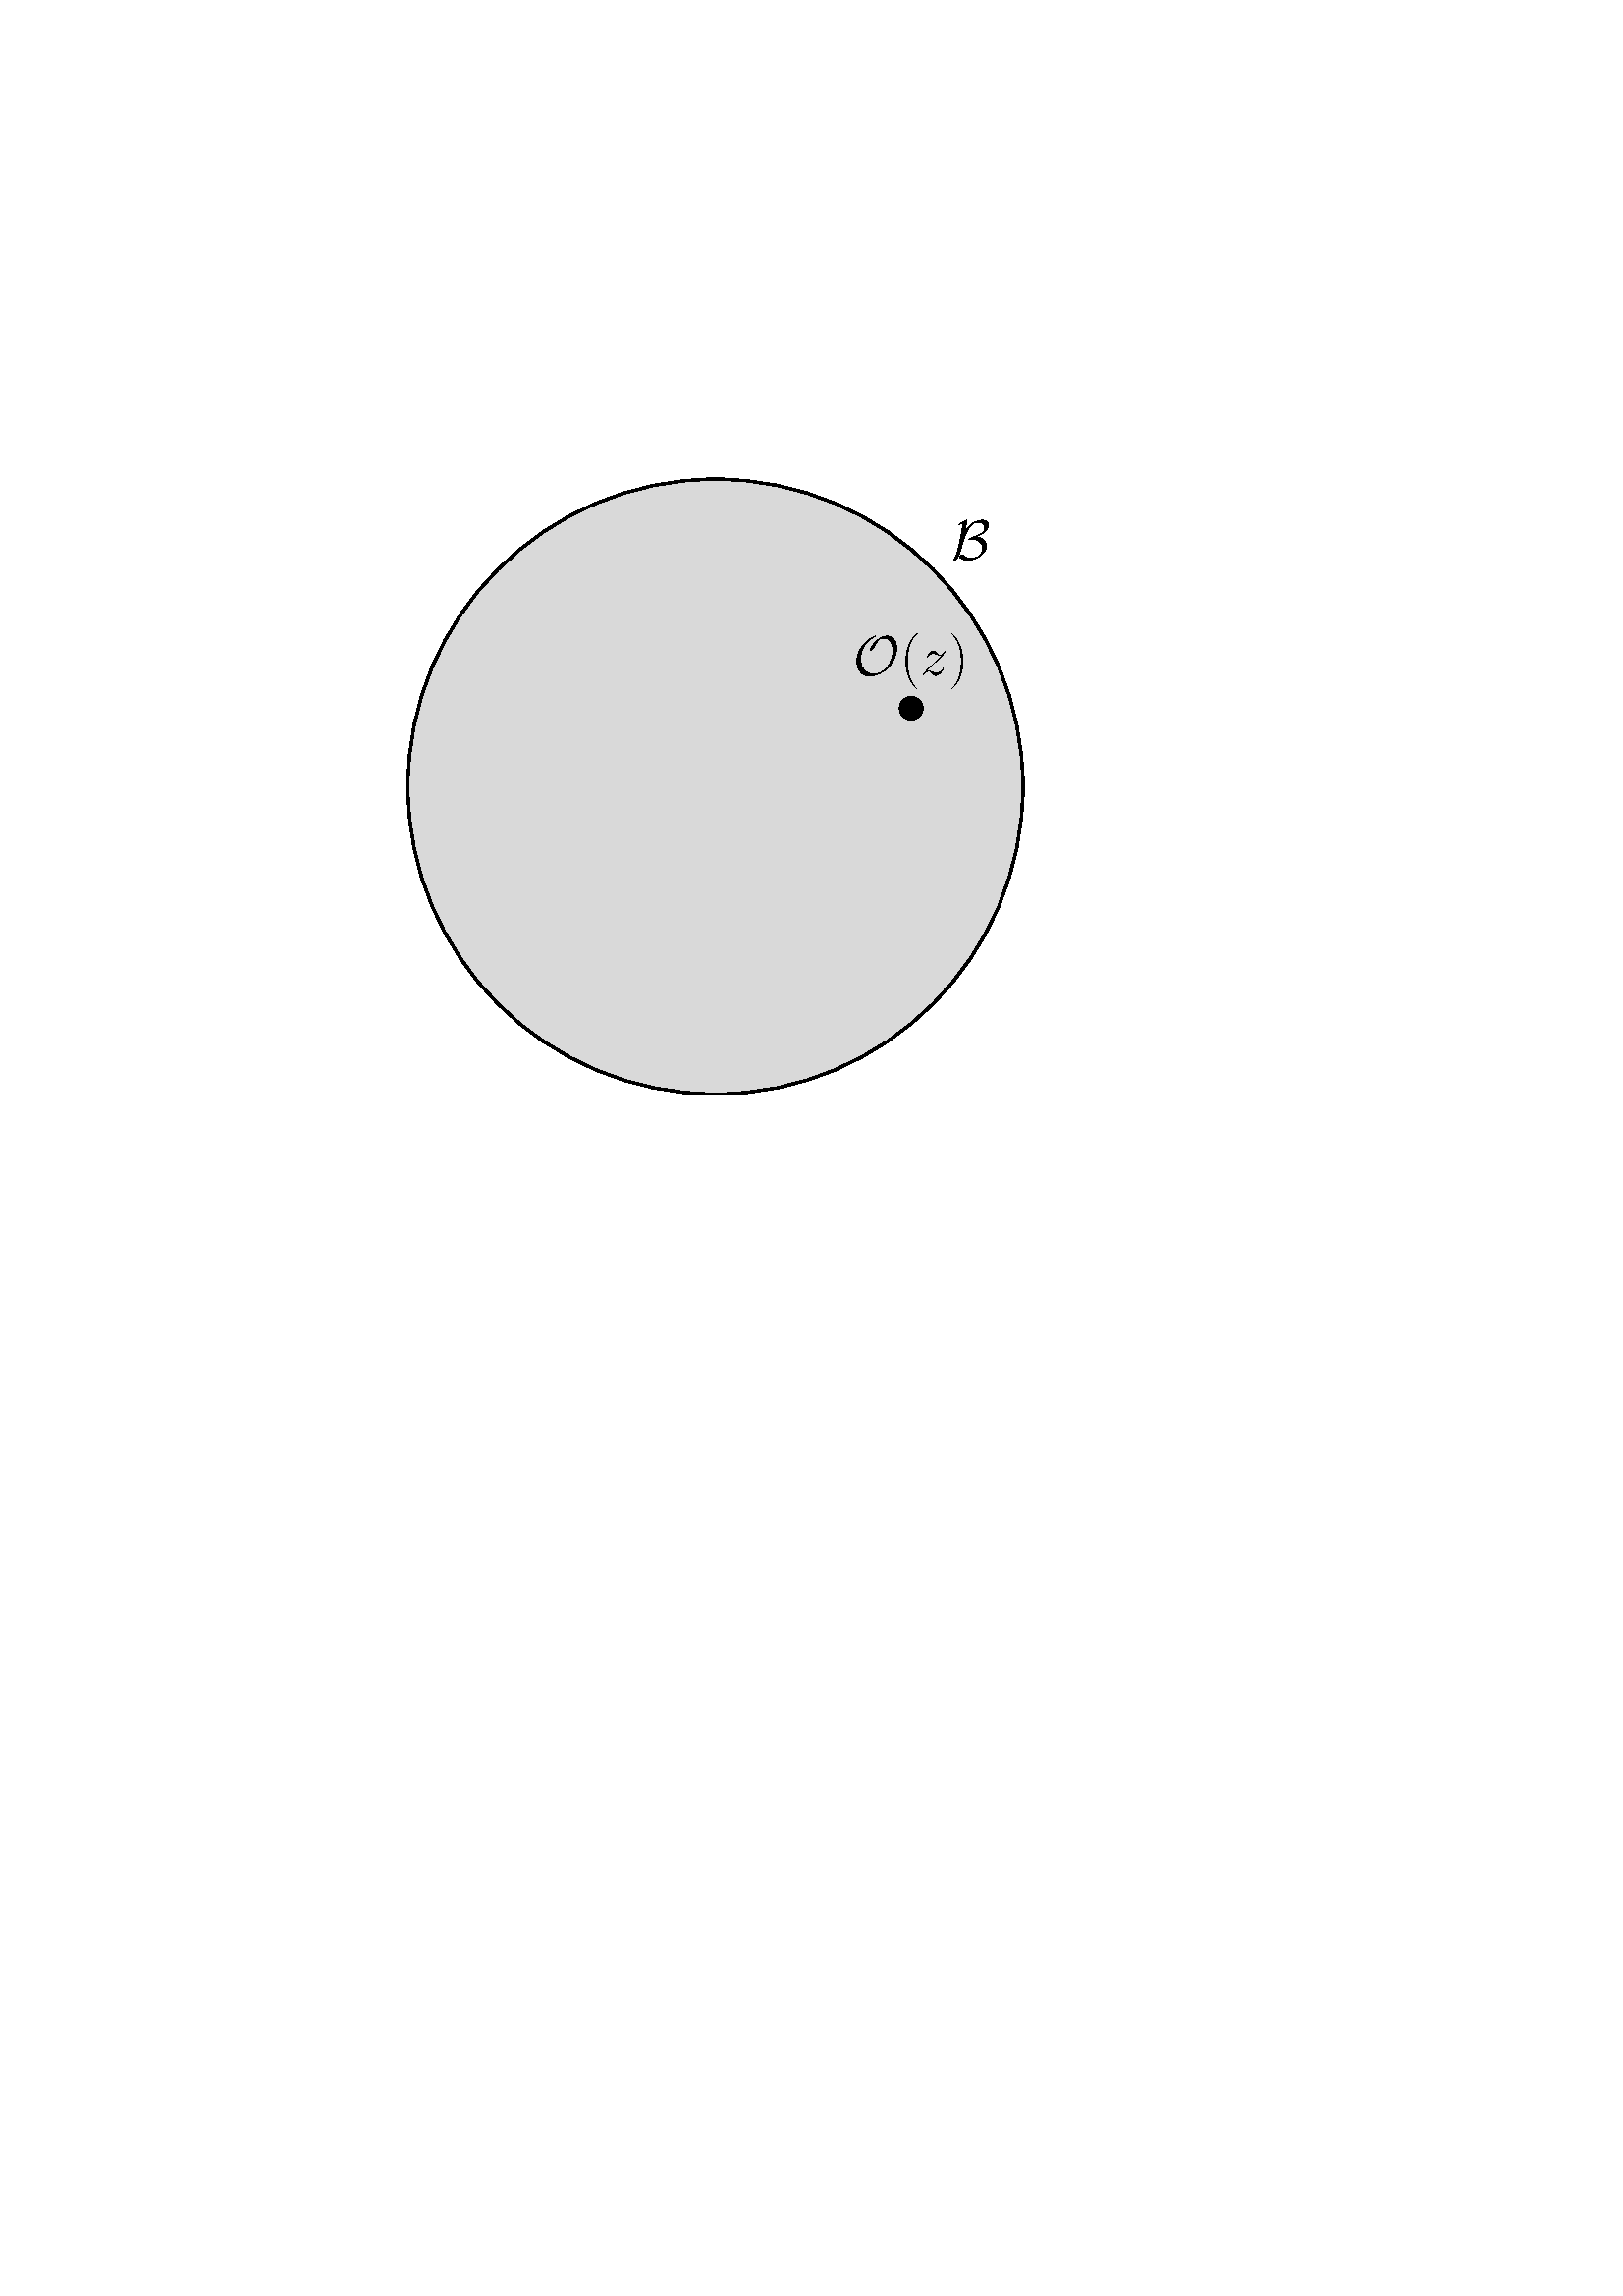
\includegraphics[width=0.75\linewidth]{figures/gla3-1.png}
\caption{ \medskip 在圆盘（阴影区域）内部一点 $z$ 处插入的局部算子 ${\EUO}(z)$，该圆盘的边界由膜 ${\cal B}$ 标记。当 $z$ 趋近圆盘边界时，${\EUO}(z)$ 可能趋于一个复常数。若对适当的算子 ${\EUO}_{H_\alpha}$ 这一点成立，我们就说 ${\cal B}$ 支撑在 Hitchin 纤维化的纤维 $\CMF$ 上。（原文 Fig.~3）}
\label{fig:trampo}
\end{figure}

由于零膜支撑在单个点上，它位于 Hitchin 纤维化的单根纤维 $\CMF_p$ 上。这根纤维由方程 $H_\alpha = h_\alpha$ 刻画，其中 $H_\alpha$ 是相互对易的哈密顿量，$h_\alpha$ 是复常数。在量子层面，我们说膜 ${\cal B}$ 支撑在纤维 ${\CMF}_p$ 上，如果当 $z$ 趋近由膜 ${\cal B}$ 标记的边界时，算子 ${\EUO}_{H_\alpha}(z)$ 趋于 $c$-数 $h_\alpha$（\trampo）。膜 ${\cal B}_p$ 当然具有这一性质。

现在我们考虑对偶运算 $S$。它把 $G$ 换成 Langlands 对偶群 $^L\negthinspace G$，从而把零膜 ${\cal B}_p$ 变成靶空间为 $\MH(^L\negthinspace G,C)$ 的 sigma 模型中的对偶膜 $\tilde{\cal B}_p$。回看表 2，我们看到，由于 ${\cal B}_p$ 是 $(B,B,B)$ 型膜，$\tilde {\cal B}_p$ 将是 $(B,A,A)$ 型膜，即在复结构 $I$ 中为 $B$-膜、在复结构 $J$ 与 $K$ 中为 $A$-膜。

变换 $S$ 给出映射 $\Xi:{\EUBB}\to {}^L\negthinspace{\EUBB}$，其中 ${\EUBB}$ 是 $G$ 的 Hitchin 纤维化的基，$^L\negthinspace{\EUBB}$ 是 $^L\negthinspace G$ 的相应基。具体地说，若点 $v\in {\EUBB}$ 由方程 $H_\alpha-h_\alpha=0$ 定义，而 $S$ 把 $H_{\alpha}$ 映到 $^LH_{\alpha}$，则 $\Xi(v)$ 由方程 $^LH_\alpha-h_\alpha=0$ 定义。如上所述，对单连通型 $G$，映射 $\Xi$ 是恒等映射。

把 $S$ 应用到 \trampo 的情形，我们观察到：若对膜 ${\cal B}$，算子 ${\EUO}_{H_\alpha}(z)$ 当 $z$ 趋近边界时趋于 $h_\alpha$，则对对偶膜 $\tilde {\cal B}$，对偶算子 ${\EUO}_{\tilde H_\alpha}(z)$ 在同一极限下同样趋于 $h_\alpha$。因此，若膜 ${\cal B}$ 支撑在 $G$ 的 Hitchin 纤维化的纤维 ${\CMF}$ 上，则其 $S$-对偶是支撑在 $^L\negthinspace G$ 的 Hitchin 纤维化的相应纤维 $\tilde {\CMF}=\Xi({\CMF})$ 上的膜 $\tilde {\cal B}$。

因此，$\tilde{\cal B}_p$ 是 $(B,A,A)$ 型膜，且支撑在对偶 Hitchin 纤维化的纤维 $\tilde {\CMF}$ 上。让我们聚焦于 $\tilde{\cal B}_p$ 为 $A$-膜的那些复结构 $J$ 与 $K$。一般地，空间 $X$ 中 $A$-膜的支撑至少是中间维数的。最熟悉的 $A$-膜支撑在中间维数的 Lagrangian 子流形上；也存在更奇异的余各向同性（coisotropic）$A$-膜，其支撑高于中间维数 \cite{ref80}。但中间维数是 $A$-膜支撑维数的下界。

然而，像 $\tilde {\cal B}_p$ 这样支撑在纤维 $\tilde {\CMF}$ 上的 $A$-膜，其支撑 {\it 至多} 是中间维数的。为调和这些约束，$\tilde{\cal B}_p$ 的支撑必须恰好是 $\tilde {\CMF}$。的确，如第~\ref{sec:hitchfib}~节所解释，$\tilde {\CMF}$ 在复结构 $I$ 中全纯，并且关于辛结构 $\omega_J$ 与 $\omega_K$ 是 Lagrangian 的。所以包在 $\tilde {\CMF}$ 上、并带有平坦酉 Chan-Paton 丛 ${\cal L}$ 的膜确实是 $(B,A,A)$ 型膜。

下面我们比较两边的模空间，只限于一边支撑在 ${\CMF}$ 上或另一边支撑在 $\tilde {\CMF}$ 上的膜。在这一限制下，${\cal B}_p$ 的模空间就是 ${\CMF}$ 的一份拷贝：$p$ 可以是 ${\CMF}$ 中任意点。

与此同时，对偶膜 $\tilde{\cal B}_p$ 的模空间是复环面 ${\EUJ}_{\tilde {\CMF}}$，它参数化 $\tilde {\CMF}$ 上秩为 1 的平坦 Chan-Paton 丛。（秩为 1，否则 $\tilde{\cal B}_p$ 的模空间维数将大于 ${\cal B}_p$ 的，$S$-对偶就不能成立。）${\EUJ}_{\tilde {\CMF}}$ 与 ${\CMF}$ 或 $\tilde {\CMF}$ 维数相同。显然，$S$-对偶在 ${\CMF}$ 与 ${\EUJ}_{\tilde {\CMF}}$ 之间建立同构。

当然，我们也可以反向进行。$\MH(^L\negthinspace G,C)$ 中位于 $\tilde {\CMF}$ 上一点处的零膜，同样被 $S$ 变换为 $\MH(G,C)$ 中包在 ${\CMF}$ 上、并带有平坦酉 Chan-Paton 丛的膜。所以 $S$-对偶同样在 $\tilde {\CMF}$ 与 ${\EUJ}_{\CMF}$（${\CMF}$ 上秩为 1 的平坦 Chan-Paton 丛的模空间）之间建立同构。

这幅图景就是环面纤维化之间的 SYZ 对偶。${\CMF}$ 参数化 $\tilde {\CMF}$ 上秩为 1 的平坦 Chan-Paton 丛，反之亦然。非正式地说，我们可以这样描述：运算 $S$ 通过映射 $\Xi:{\EUBB}\to{}^L\negthinspace{\EUBB}$（从一个 Hitchin 纤维化的基到对偶纤维化的基）连同在相应环面纤维上的 $T$-对偶来作用。这就是镜像对称通常的 SYZ 图景，只不过映射 $\Xi$ 通常被假定为平凡。

\begin{yizhu}[物理图像]
按：SYZ 图景把镜像对称拆成两部分：底空间之间一个通常取为恒等的映射，以及纤维环面之间的 $T$-对偶。对 Hitchin 纤维化，这个底映射恰好是四维 $S$-对偶在基上的经典作用 $\Xi$，对 simply-laced $G$ 取恒等；而纤维上的 $T$-对偶对应零膜到包在纤维上的膜的转换。这就是本节开头「在基上经典地作用、在纤维上通过 $T$-对偶作用」的精确含义。
\end{yizhu}

对酉群，$G$ 与 $^L\negthinspace G$ 的 Hitchin 纤维化的相应纤维互为对偶复环面，这一点已由 Hausel 与 Thaddeus \cite{ref21} 证明。对例外 Lie 群 $G_2$，Hitchin 最近建立了这一对偶 \cite{ref81}。Donagi 与 Pantev 用谱覆盖的抽象方法对任意半单 Lie 群分析了这一问题 \cite{ref82}。另见 Faltings 关于 $G$-丛的工作 \cite{ref83}。

在这一解释中，我们略去了关于该对偶的若干重要微妙之处。有些问题涉及 $G$ 的中心与基本群，在第~\ref{sec:centertop}~节有简要讨论。另一些问题涉及 $C$ 上自旋结构的作用，本文不分析。关于自旋结构的作用，以及中心与基本群的作用、酉群情形的对偶的更多细节，将另文发表 \cite{ref26}。

\subsection{$\MH$ 上的膜}

\label{sec:mhbranes}

我们已经遇到 $\MH$ 上膜的若干有趣例子——零膜与包在纤维上的膜。我们还会遇到其他例子。如同最初的例子，大多数重要的膜将关于三个复结构 $I$、$J$、$K$ 都具有超对称性质，这在理解它们的行为时非常有用。最令人感兴趣的膜保持有效二维 sigma 模型的一半超对称，而后者又具有底层规范场论的一半超对称。

例子包括 $(B,B,B)$-膜，即在每个复结构 $I,J,K$ 中都是 $B$-膜的膜，以及 $(B,A,A)$、$(A,B,A)$、$(A,A,B)$ 型膜，它们在一个复结构中为 $B$-型、在另外两个中为 $A$-型。我们已经看到 $S$ 把一个 $(B,B,B)$ 型膜与一个 $(B,A,A)$ 型膜互换。由表 2 还可看出，$S$ 把 $(A,B,A)$ 型膜映到同型的另一个膜，$(A,A,B)$ 型膜亦然。

给出这四种类型膜的例子并不困难；它们将是我们研究几何 Langlands 纲领时的重要膜。当然，更一般地，可以有这样的膜：它对复结构 $I,J,K$ 的任意线性组合为 $B$-型，而对两个正交的复结构为 $A$-型。\footnote{然而，不存在 $(B,B,A)$ 型膜。在复结构 $I$ 与 $J$ 中全纯的子簇自动在复结构 $K$ 中全纯。同样也不存在 $(A,A,A)$ 型膜。}

\begin{yizhu}[易错点]
按：膜类型的三个字母按复结构 $(I,J,K)$ 的次序排列，$B$/$A$ 分别指在该复结构中为 $B$-膜/$A$-膜。脚注的两个「不存在」来自超凯勒流形的复结构关系：在 $I,J$ 中全纯自动在 $K$ 中全纯，故没有 $(B,B,A)$；对 $A$-型也不可能有三个方向同时成立，故没有 $(A,A,A)$。
\end{yizhu}

我们已经研究过的零膜是最显然的 $(B,B,B)$ 型膜。$(B,B,B)$-膜的其他例子是填满空间的膜，其靶空间是整个 $\MH$，并带有在三个复结构中每一个都全纯的 Chan-Paton 向量丛。这类丛包括平凡丛，也包括其他例子，它们在几何 Langlands 纲领中的作用将另文讨论 \cite{ref26}。

一大类 $(B,A,A)$-膜的例子如下。设 $N$ 是 $\MH$ 在复结构 $I$ 中的复子流形，它关于全纯辛结构 $\Omega_I$、从而关于 $\omega_J$ 与 $\omega_K$ 是 Lagrangian 子流形。则支撑在 $N$ 上、带有平凡 Chan-Paton 丛的膜是 $(B,A,A)$-膜。我们已经遇到一个重要例子：$N$ 可以是 Hitchin 纤维化的纤维。另一个例子是，从复结构 $I$ 的角度，取 $N$ 为所有对 $(E,\varphi)$ 构成的空间，其中 $E$ 固定而 $\varphi$ 可变。从规范场论的观点，这意味着 $A_{\bar z}$ 在规范变换下固定，从而保证 $\Omega_I=(1/\pi)\int_C\,|d^2z|\,\Tr\,\delta\phi_z\wedge\delta A_{\bar z}$ 的消失。因此这给出 $(B,A,A)$ 型膜。

类似地，$(A,B,A)$ 与 $(A,A,B)$-膜的例子来自关于复结构 $J$ 或 $K$ 的复 Lagrangian 流形。复结构 $J$ 中复 Lagrangian 流形的一个简单例子，只需保持 ${\cal A}_{\bar z}=A_{\bar z}+ i\phi_{\bar z}$ 固定而让 ${\cal A}_z=A_z+i\phi_z$ 变化即可得到。这给出具有指定全纯结构的所有平坦 $G_{{\Bbb{C}}}$ 丛构成的族。类似地，通过指定 $A_{\bar z}-\phi_{\bar z}$ 并让 $A_z+\phi_z$ 变化，我们得到复结构 $K$ 中的复 Lagrangian 流形。在第~\ref{sec:abranes}~节，我们将把 $(A,B,A)$ 或 $(A,A,B)$ 型膜的更精细例子构造成「余各向同性膜」。

\section{圈算子与线算子}

\label{sec:loopop} 

\begin{keytakeaways}
\begin{itemize}[leftmargin=1.4em,itemsep=2pt,topsep=2pt]
\item \textbf{物理图像}：本节讨论的四维 TQFT 允许插入与定向一维子流形 ${\cal S}\subset M$ 相联系的算子。这些算子的参数不是普通的「点」，而是环路或通向无穷远的线，因而被称为圈算子与线算子。
\item \textbf{数学工具}：这类算子依赖 ${\cal S}$ 的同伦类而不只是同调类；在 $t=\pm i$ 处，可以用 $A$ 与标量场 $\phi$ 的复化联络 $\CA=A+i\phi$（或 $\overline\CA=A-i\phi$）的 holonomy 构造具有拓扑对称性的 Wilson 算子。
\item \textbf{关键结论}：Wilson 算子是四维理论中最基本的圈算子；它的磁对偶 't Hooft 算子将在第~\ref{sec:tophooft}~节引入。紧化到二维后，线算子可以被解释为作用在膜上的算子，这正是通向几何 Langlands 纲领的入口。
\item \textbf{边界与展望}：对有端点或通向无穷远的线算子须小心处理；在非紧四维流形上，静态线算子必须纳入量子化以构造物理态空间，这是本文应用中最重要的情况。
\end{itemize}
\end{keytakeaways}

与第~\ref{sec:twisting}~节引入的四维 TQFT 表面上来源相似的其他理论相比，这些 TQFT 真正特别之处在于：它们允许与定向一维流形 ${\cal S}\subset M$ 相联系的算子，而且这些算子依赖 ${\cal S}$ 的同伦类，而不只是同调类。要点并不是我们想研究 $M$ 的基本群，而是这些一维流形算子在关于膜的问题上被证明具有非常有趣的性质。

若 $M$ 是紧的且没有边界，则要求 ${\cal S}$ 是闭圈。为反映这一情形，一维流形算子通常被称为圈算子。然而更一般地，在非紧四维流形上，我们允许通向无穷远的线算子。一个重要的例子是静态线算子，其轨迹在空间中某个固定点处贯穿全部时间。在量子化理论以构造物理态空间时，必须把这样的线算子包括进来。这实际上将是我们应用中最重要的情况。\footnote{因此，其他情形——例如终止在膜上的线算子——虽然在一般情况下有意义，但在本文中并不重要。}

% 说明：以下四行是脚手架把原文的 \nref 文献定义转成的 \cite；原文此处并不产生引用标记，
% 这些文献在下文已有正常引用。为保持 \cite 计数与 skel 一致，此处按注释保留。
% \cite{ref84}
% \cite{ref85}
% 
% 

在第~\ref{sec:topwil}~节，我们讨论最基本的圈算子或线算子，通常称为 Wilson 算子。在与本文所考虑的理论类似的 TQFT 中，Wilson 算子最早由 Blau 与 Thompson 构造 ，其中的联络被一个标量场修改以保证拓扑对称性。类似的规范不变算子也被用于研究五维超对称杨--米尔斯理论 。这类算子在弦论的当代进展中是重要的（连同它们的磁对偶，我们将在第~\ref{sec:tophooft}~节引入）。它们最早是在半 BPS 情形下被引入的 \cite{ref86,ref87}。我们所考虑的拓扑线算子，与 \cite{ref88} 中对任意环路 ${\cal S}\subset \Bbb{R}^4$ 定义的 1/16 BPS 线算子最为相似。

\begin{yizhu}[含糊点拨]
按：「依赖同伦类而非同调类」是本节标题所示算子的关键特征：算子的插入位置是 $M$ 中带定向的一维子流形，拓扑对称性使关联函数只依赖其同伦类。原文特意声明这并不是要研究 $\pi_1(M)$——研究基本群本身没有意义，有意义的是这类算子与膜的关系，后文会看到它们变成膜范畴上的函子。
\end{yizhu}

在第~\ref{sec:tophooft}~节，我们描述对偶的 't Hooft 算子。在第~\ref{sec:comptwo}~节，我们讨论这类算子在紧化到二维后的解释。最后，在第~\ref{sec:lineop}~节，我们把线算子作为膜上的算子来研究。

\subsection{拓扑 Wilson 算子}

\label{sec:topwil}

在规范场论中，最基本的圈算子是 Wilson 圈算子。我们考虑规范群为 $G$、$G$-丛 $E\to M$ 上的联络为 $A$ 的规范场论。令 ${\cal S}$ 是 $M$ 中的定向闭圈，其定向比如说由选取一个一形式 $ds$ 给出，其中 $s$ 是沿 ${\cal S}$ 的参数。我们取定 $G$ 的一个不可约表示 $R$，并令\footnote{由于我们的协变导数为 $D=d+A$，holonomy 算子在指数上带一个负号。用 hermitian 规范场 $A'=iA$（回忆式 \eqref{eq:boloko}）表述时，holonomy 算子为 ${\rm Tr}_R\,P\,\exp\left(i\oint_{\cal S} A'\right)$。}
% [WARN] 公式 \eqn\eqref{eq:ytro} 无编号或重复
\begin{equation*}
\tag*{(6.1)}
W_0(R,{{\cal S}})={\rm Tr}_R
\,P\,\exp\left(-\oint_{{\cal S}} A\right).
\end{equation*}
换言之，$W_0(R,{\cal S})$ 是 $A$ 绕 ${\cal S}$ 的 holonomy 在表示 $R$ 中的迹。

\begin{yizhu}[易错点]
按：式 (6.1) 指数上的负号来自协变导数约定 $D=d+A$（见脚注），换成 hermitian 规范场 $A'=iA$ 后就是通常的 ${\rm Tr}_R P\exp(i\oint A')$。这里的 $W_0$ 还是普通（未扭化）的 Wilson 圈算子；它一般不具有拓扑对称性，正是下面要修改的对象。
\end{yizhu}

现在我们回看第~\ref{sec:twisting}~节中的式 \eqref{eq:bono}，其中我们确定了 $A$ 在拓扑对称性下的变换规律：% 式 (6.2)
\setcounter{equation}{1}
\begin{equation}\label{eq:likp}
\delta_T
A_\mu=iu\psi_\mu+iv\tilde\psi_\mu.
\end{equation}
显然，对任意非零的 $(u,v)$，Wilson 圈算子不是不变的。然而，扭化的 ${\EUN}=4$ 杨--米尔斯理论还有一个伴随值的一形式 $\phi=\sum_{\mu=0}^3\phi_\mu\,dx^\mu$，其变换为
% 式 (6.3)
\setcounter{equation}{2}
\begin{equation}\label{eq:nikp}
\delta_T\phi_\mu=iv\psi_\mu-iu\tilde\psi_\mu.
\end{equation}
可以通过给联络 $A$ 加上 $\phi$ 的一个倍数来修改它。

确切地说，当 $t=v/u$ 等于 $\pm i$ 时，$A$ 与 $\phi$ 的一个线性组合是不变的。对 $t=i$，不变的组合是 $\CA=A+i\phi$；在 $t=-i$ 时，它是 $\overline\CA=A-i\phi$。于是我们把超对称 Wilson 圈算子定义为 $\CA$ 或 $\overline\CA$ 绕 ${\cal S}$ 的 holonomy。因此
% 式 (6.4)
\setcounter{equation}{3}
\begin{equation}\label{eq:ymop}
W(R,{\cal S})=\Tr_R\,P\exp\left(-\oint_{{\cal
S}}\CA\right)=\Tr_R\,P\exp\left(-\oint_{{\cal
S}}(A+i\phi)\right),~~ t=i
\end{equation}
以及 % 式 (6.5)
\setcounter{equation}{4}
\begin{equation}\label{eq:jymop}
W(R,{{\cal S}})=
\Tr_R\,P\exp\left(-\oint_{{\cal S}}{\overline\CA}\right)
=\Tr_R\,P\exp\left(-\oint_{{\cal S}}(A-i\phi)\right), ~~t=-i.
\end{equation}
$SU(4)_{{\cal R}}$ 的中心生成元 $\EUI$ 通过 $t\to -t$ 与 $\phi\to -\phi$ 作用，把其中一个公式变成另一个。

\begin{yizhu}[物理图像]
按：$t=\pm i$ 是 GL 扭化的两个特殊点：此时拓扑超荷的组合恰好使 $A\pm i\phi$ 不变，于是可以取它的 holonomy 作为拓扑不变的圈算子。$\CA=A+i\phi$ 正是 Hitchin 方程中出现的复化联络；在 $t=i$ 时拓扑方程 \eqref{eq:loopme} 断言 $\CA$ 平坦，这与后面把 Wilson 算子解释为膜上的算子密切相关。
\end{yizhu}

在 $t=\pm i$ 时，具有拓扑对称性的 Wilson 圈算子的存在是极其自然的。在这些 $t$ 值下，拓扑方程 \eqref{eq:loopme}\ 断言 $\CA$ 的平坦性。所以 $\CA$ 或 $\bar\CA$ 绕闭圈的 holonomy 是自然的不变量。同样地，若 $t\not=\pm i$，这类 holonomy 不是自然的不变量，因为拓扑方程不一定蕴含平坦性。（第~\ref{sec:vanishing}~节的消灭定理把超对称位形与一般 $t$ 下的复平坦联络联系起来，但它们需要某些整体输入，并不在所有情形下成立，例如涉及可能应用该 TQFT 的膜时。）

\begin{yizhu}[易错点]
按：$-i$ 与 $+i$ 给出的两个公式由 $\EUI$ 互换，注意不要漏掉 $t\not=\pm i$ 的例外：此时 $\CA$ 或 $\bar\CA$ 的 holonomy 不是拓扑不变量。括号内的提醒也很重要——消灭定理（把超对称位形等同于复平坦联络）依赖整体性假设，在有膜的情形可能失效，这一点在后文把线算子变成膜上算子时会反复用到。
\end{yizhu}

虽然我们是对闭圈 ${\cal S}$ 表述这些定义的，但它们在开曲线情形有很好的类比。若 ${\cal S}$ 的端点为 $p$ 与 $q$，我们就把 $W(R,{{\cal S}})$ 不定义为迹，而定义为从 $p$ 处 $E$ 的纤维（在表示 $R$ 中取）到 $q$ 处纤维的平行移动（关于联络 $\CA$ 或 $\bar\CA$）矩阵。于是 $W(R,{{\cal S}})$ 是从 $p$ 处的向量空间到 $q$ 处的向量空间的映射。它随后被纳入一个更大的量子构造，涉及初始与最终的量子态，正如我们在引言中所提到的。当我们真正进入几何 Langlands 纲领时，Wilson 算子的这个推广版本将是必不可少的。

\begin{yizhu}[物理图像]
按：开曲线情形把 Wilson 算子从「一个数」（迹）升级为「一个矩阵」（平行移动），从而可以作用在边界态空间上。这正是「线算子作为膜上的算子」的技术雏形：线算子的两个端点可以贴在膜上（或对应初始/末态），于是它的作用变成膜上态空间之间的映射，后文将把它实现为 Hecke 算子之类的函子。
\end{yizhu}

上下文清楚时，我们把 $W(R,{{\cal S}})$ 简写为 $W(R)$ 或干脆写 $W$。

%% ============================================================
%% 分片 16：原文第 6 节「Loop and Line Operators」（原文 glshort.tex 起于第 4483 行）
%% 由 tools/harvmac2tex.py 从 arXiv 源码（hep-th/0604151v3）自动生成。
%% 只译英文散文；公式、编号、\label、\cite 一律不改。
%% ============================================================

\subsection{拓扑 't Hooft 算子}

\label{sec:tophooft}

我们已在 $t=\pm i$、即 $\Psi=\infty$ 处的拓扑场论中找到了 Wilson 算子。按 $S$-对偶 $S:\Psi\to -1/n_{\frak g}\Psi$，在 $\Psi=0$ 处必定存在对偶的算子。拓扑 Wilson 算子是由 $G$ 的一个表示 $R$ 的选择来分类的。因此，既然 $S$ 交换 $G$ 与 $^L\negthinspace G$，那么出现在 $\Psi=0$ 处 TQFT 中的对偶算子就必须由 $^L\negthinspace G$ 的一个表示 $^L\negthinspace R$ 来分类。

Wilson 算子就是统计力学中常说的「有序」（order）算子的一个例子。有序算子由某个经典表达式（例如联络绕一个圈的和乐）构造，随后被解释为量子算子，并作为一项因子纳入路径积分。

有序算子的对偶常常是「无序」（disorder）算子。无序算子是通过指定经典场所应具有的奇异性来定义的，并在该奇异性存在的情况下作路径积分（或量子化）。在经典层面，有序算子与无序算子看起来像是完全不同类型的对象。但在量子层面，在适当的情形下它们具有相同的形式性质，并且常常被对偶互换。在我们的问题中，Wilson 算子的对偶是 't Hooft 算子，它是无序算子的一个例子。\footnote{关于在 $G=U(1)$ 情形下 Wilson 算子的对偶确为 't Hooft 算子的一个显式论证，见 \cite{ref89}。}

要定义与一个圈 ${\cal S}\subset M$ 相伴的 Wilson 圈算子，我们需要 ${\cal S}$ 的一个定向。't Hooft 圈算子需要的则是 ${\cal S}$ 的法丛的一个定向。事实上，方便的做法是把 ${\cal S}$ 的一个小邻域等同于 ${\cal S}\times \Bbb{R}^3$，并记 $\epsilon_3$ 为 $\Bbb{R}^3$ 上的一个体积形式。't Hooft 算子的定义只依赖于法丛的定向，而不依赖于这些选择的细节。若 $r$ 表示到 ${\cal S}$ 的距离（在某个度规下），则我们也可以写 % 式 (6.6)
\setcounter{equation}{5}
\begin{equation}\label{eq:congo}
\epsilon_3=dr\,d{\rm
Vol},
\end{equation}
 其中 $d{\rm Vol}$ 是固定 $r$ 处的二维球面上的体积形式。

在本文中，当我们就 $U(N)$ 或 $SU(N)$ 规范理论中的 't Hooft 算子写出显式公式时，我们把规范场看作秩 $N$ 向量丛上的联络。这意味着 $A$ 与 $\phi$ 是取值为 $N\times N$ 反 Hermite 矩阵的 1-形式；当 $N=1$ 时，它们就简单地是虚 1-形式。

让我们先描述 $U(1)$ 规范理论中最基本的 't Hooft 算子。在 $\Bbb{R}^4=\Bbb{R}\times \Bbb{R}^3$ 上取坐标 $(s,\vec x)$。奇异的 Dirac 单极子是 Maxwell 方程的一个经典解，它在 $s$ 的平移下以及 $\vec x$ 的旋转下不变，并在由 $\vec x=0$ 定义的直线 $L$ 上有奇异性。若 $F=dA$ 是 $U(1)$ 联络 $A$ 的曲率，则 Maxwell 方程读作 $dF=d\star F=0$，而它可以在 $\Bbb{R}^3\backslash \{0\}$ 上（即在 $\Bbb{R}^3$ 中挖去点 $\vec x=0$ 之后）由下式求解 % 式 (6.7)
\setcounter{equation}{6}
\begin{equation}\label{eq:izo}
F={i\over 2}\star d\left({1\over |\vec
x|}\right).
\end{equation}
  使用 Hodge $\star$ 算子显式地显示出对 $L$ 的法丛定向的依赖。要得到 $\Bbb{R}^4\backslash L$ 上的解，只需利用投影 $\Bbb{R}^4\backslash L\to \Bbb{R}^3\backslash \{0\}$，把 $F$ 拉回到 $\Bbb{R}^4\backslash L$ 上，作为 Maxwell 方程的解。
 $F$ 已被归一化，使得若 $Y$ 是包围 $\vec x=0$ 处奇异性的二维球面，则 $\int_Y \,iF/2\pi =1$。因此存在一个酉线丛 ${\cal L}\to \Bbb{R}^4\backslash L$，它容许一个曲率为 $F$ 的联络。这就是奇异的 Dirac 单极子。它以 $\int_Yc_1({\cal L})=1$ 为特征。

阿贝尔规范理论中最基本的 't Hooft 算子的定义是：路径积分须在 $\Bbb{R}^4\backslash L$ 上的线丛的联络上进行，而这些联络在 $L$ 附近与奇异的 Dirac 单极子相符。这里没有必要只考虑直线。$L$ 可以换成一般四维流形 $M$ 中任意一条闭曲线 ${{\cal S}}$，或者（若 $M$ 是测地完备的）换成任意一条通向无穷远的曲线。在曲线 ${{\cal S}}$ 上插入 't Hooft 圈算子 $T_{(0)}$ 的路径积分，是通过对 $M\backslash {{\cal S}}$ 上的阿贝尔规范场\footnote{若 ${\cal S}$ 在 $H_1(M,\Bbb{Z})$ 中的同调类非零，则不存在这样的阿贝尔规范场，我们规定该路径积分为零。其对偶的说法是：若 ${\cal S}$ 的同调类非零，则 Wilson 算子 $W(R,{\cal S})$ 在对所有联络积分之后的期望值为零；这一为零来自用平坦线丛作扭化时的行为。}作路径积分而得到的，并要求曲率在 ${{\cal S}}$ 附近发散如 $F\sim {i\over 2}\star_3d (1/r)$，其中 $r=|\vec x|$ 现在是到 ${{\cal S}}$ 的距离，而 $\star_3$ 是作用在形式上的一个运算，它在 ${{\cal S}}$ 附近看起来就像法向于 ${{\cal S}}$ 的平面上的 $\star$ 算子。更一般地，取定一个整数 $m$ 并要求 $F$ 的奇异部分为 $F\sim{(im/ 2)}\star_3 d (1/r)$，就得到电荷为 $m$ 的 't Hooft 圈算子 $T_{(0)}(m)$。

现在让我们考虑规范群为 $U(1)$ 的 ${\EUN}=4$ 超对称杨–米尔斯理论。我们可以要求规范场具有 Dirac 单极子奇异性、而其余场非奇异，以此定义一个 't Hooft 算子。但这样的算子与 $\Psi=0$ 处的拓扑对称相容吗？

我们可以如下判定这个问题。要到达 $\Psi=0$，我们取 $t=1$ 且 $\tau$ 为虚数。为使 't Hooft 算子保持拓扑对称，场在 ${{\cal S}}$ 附近的奇异行为必须与该对称相容。由于问题只涉及 ${{\cal S}}$ 附近的局部行为，方便的做法是暂时回到 ${{\cal S}}$ 为 $\Bbb{R}^4$ 中直线 $L$ 的情形。

 一组场 $(A,\phi)$ 保持拓扑对称的条件已在式 \eqref{eq:loopme} 中求出。若这些方程与 't Hooft 算子所要求的那类奇异性相容，则 't Hooft 算子保持超对称。否则，在 't Hooft 算子存在时任何场组态都不可能超对称，我们就说 't Hooft 算子破坏超对称。

在 $t=1$ 且对阿贝尔规范理论，所需条件读作 % 式 (6.8)
\setcounter{equation}{7}
\begin{equation}\label{eq:nurot}
(F+d\phi)^+=(F-d\phi)^-=0.
\end{equation}
 若 $F$ 具有 Dirac 单极子奇异性而 $\phi$ 非奇异，这些方程就不被满足。要得到保持拓扑对称的 't Hooft 算子，正如 Wilson 的情形一样，我们必须以适当的方式把 $\phi$ 包含进来。

为使方程 \eqref{eq:nurot}\ 得到满足，$\phi$ 必须伴随 $F$ 的 Dirac 单极子奇异性而具有何种奇异性？这个问题有一个简单的答案：我们应取 $\phi=(i/2|\vec x|)ds$，其中 $s$ 是沿 $L$ 的「时间」坐标。于是，若取
% 式 (6.9)
\setcounter{equation}{8}
\begin{equation}\label{eq:hildo}
\begin{aligned}F& ={i\over 2}\star_3 d{1\over |\vec x|}\\
                    \phi& = {i\over 2|\vec x|} ds,\\\end{aligned}
\end{equation}

其中 $\star_3$ 是沿法向于 $L$ 的方向的三维 Hodge $\star$ 算子。

这就告诉我们，对于一般的闭一维流形 ${{\cal S}}\subset M$，如何定义在 $\Psi=0$ 处保持拓扑对称的基本 't Hooft 算子 $T$：要计算该算子的矩阵元，就对在 ${{\cal S}}$ 附近具有 \eqref{eq:hildo} 所描述奇异性的场作路径积分。类似地，对任意整数 $m$，要得到电荷为 $m$ 的拓扑 't Hooft 算子 $T(m)$，只需要求场沿 ${{\cal S}}$ 的奇异性是 \eqref{eq:hildo} 所描述奇异性的 $m$ 倍。

\par\medskip{\it 推广到任意 $G$ 与 Langlands 对偶}

下一步是把这一构造推广到任意 $G$。这可以简单地做到 \cite{ref90}。我们只需任取一个同态 $\rho:U(1)\to G$，然后要求场沿 ${{\cal S}}$ 的奇异性看起来像 \eqref{eq:hildo} 中奇异性在 $\rho$ 下的像，以此定义拓扑 't Hooft 算子。

这样定义的算子只依赖于 $\rho$ 的共轭类。但同态 $\rho:U(1)\to G$ 的共轭类由对偶群 $^L\negthinspace G$ 的最高权来分类。换言之，它们由 $^L\negthinspace G$ 的不可约表示来分类。

因此，对 $^L\negthinspace G$ 的每个不可约表示 $^L\negthinspace R$ 以及每个一维流形 ${{\cal S}}$，我们都得到了一个拓扑 't Hooft 算子 $T({}^L\negthinspace R,{{\cal S}})$。与 Wilson 的情形一样，若上下文清楚，我们就简单地称此算子为 $T({}^L\negthinspace R)$ 或 $T$。$G$ 的 't Hooft 算子由 $^L\negthinspace G$ 的表示来分类这一事实，就是经典的 GNO 对偶（GNO duality）\cite{ref10}，它近来被重新解释为关于算子而非态的对偶 \cite{ref90}。

't Hooft 算子的分类还与 Grothendieck 对 ${\Bbb {CP}}^1$ 上 $G$-丛的分类密切相关。按照这一分类，${\Bbb {CP}}^1$ 上的一个 $G$-丛通过一个同态 $\rho:U(1)\to G$（或其复化 $\rho:\Bbb{C}^*\to G_{\Bbb{C}}$）与基本线丛 ${\cal O}(1)\to\Bbb{CP}^1$ 相联系。我们把环绕 't Hooft 算子所定义奇异性的一个小二维球面与 $\Bbb{CP}^1$ 等同起来。黎曼面上的每个 $G$-丛，即便不稳定，也容许一个满足 Yang-Mills 方程的联络 \cite{ref91}；而在 $\Bbb{CP}^1$ 上，Yang-Mills 方程的每个解都等价于用来构造 't Hooft 算子的阿贝尔解之一。所以 't Hooft 算子的分类与 $\Bbb{CP}^1$ 上 $G$-丛的分类相同。

\par\medskip{\it 拓扑非平凡的 't Hooft 算子}

$S^2=\Bbb{CP}^1$ 上的全纯 $G$-丛在拓扑上可以非平凡，尽管 $G$-丛的拓扑分类远不如全纯分类精细。

$S^2$ 上的 $G$-丛由一个特征类 $\xi\in H^2(S^2,\pi_1(G))\cong \pi_1(G)$ 分类。但 $\pi_1(G)$ 自然同构于 $^L\negthinspace G$ 的中心。用于构造 't Hooft 算子 $T(^L\negthinspace R)$ 的 $S^2$ 上丛在拓扑上非平凡，当且仅当 $^L\negthinspace G$ 的中心在 $^L\negthinspace R$ 上非平凡地作用。

\par\medskip{\it 混合 Wilson-'t Hooft 算子：阿贝尔情形}

到目前为止，我们在 $\Psi=\infty$ 处找到了 Wilson 线算子，在 $\Psi=0$ 处找到了 't Hooft 线算子。通过施加对偶变换，我们找到 $\Psi$ 的其它特殊值，在这些值处存在保持拓扑对称的线算子。事实上，$\Psi$ 的所有有理值、并且只有这些值，可以由 $\Psi=0$（或 $\Psi=\infty$）通过对偶变换得到。无论对偶群 $\Gamma$ 是 $SL(2,\Bbb{Z})$（当 $G$ 为单边（simply-laced）型时就是如此）还是 $G$ 非单边时出现的某个 Hecke 群，这一点都成立。

要到达 $\Psi$ 的有理值，我们取 $t=1$ 且 $\theta=2\pi \Psi$。于是，我们在规范场的作用量中添加一项 % 式 (6.10)
\setcounter{equation}{9}
\begin{equation}\label{eq:into}
{{\cmmib I}}_\theta=i{\Psi\over 4\pi}\int
\Tr\,F\wedge F.
\end{equation}
 至此，有必要假定 $M$ 可定向，比如说通过选取一个体积形式 $\epsilon_4$。 ${\EUN}=4$ 超对称杨–米尔斯理论在不可定向的四维流形 $M$ 上也有意义。但我们此刻想考察其作用的相互作用 \eqref{eq:into}，只有在 $M$ 可定向时才能引入，因为定义积分 $\int_M\Tr\,F\wedge F$ 需要这一点。（更一般地，如我们在第~\ref{sec:canonpar}~节末尾所指出的，$\Psi$ 在定向反转下变号，所以要到达非零的有理 $\Psi$，我们需要 $M$ 上的一个定向。）因此我们假定 $M$ 可定向，并用体积形式 $\epsilon_4$ 的选择来表达这一方向。

定义支撑在 ${\cal S}$ 上的 Wilson 圈算子，需要用一个 1-形式 $ds$ 给出 ${\cal S}$ 的定向。定义支撑在 ${\cal S}$ 上的 't Hooft 圈算子，则需要 ${\cal S}$ 的法丛的一个定向 $\epsilon_3$。一旦 $M$ 可定向，我们就可以要求 ${\cal S}$ 的定向与其法丛的定向是相容的，即要求 % 式 (6.11)
\setcounter{equation}{10}
\begin{equation}\label{eq:delo}
\epsilon_4=ds\wedge \epsilon_3
\end{equation}
 沿 ${\cal S}$ 成立。
把 ${\cal S}$ 在 $M$ 中的一个小邻域等同于 ${\cal S}\times \Bbb{R}^3$，我们可以把 $ds$ 延拓到该邻域上，使得 \eqref{eq:delo}\ 在整个 ${\cal S}\times \Bbb{R}^3$ 上保持成立。然后如 \eqref{eq:congo} 那样写 $\epsilon_3=dr\wedge d{\rm Vol}$，我们就有 % 式 (6.12)
\setcounter{equation}{11}
\begin{equation}\label{eq:nelo}
\epsilon_4=ds\wedge dr\wedge d{\rm Vol}=-dr\wedge
ds\wedge d{\rm Vol}.
\end{equation}

在 $\Psi$ 的有理值处保持拓扑对称的线算子称为混合 Wilson-'t Hooft 算子。由于这些算子将兼具 't Hooft 算子与 Wilson 算子的性质，为定义它们，重要的是在 ${\cal S}$ 及其法丛上选取相容的定向，正如我们在上一段所做的那样。为构造这些算子，我们先考虑 $G=U(1)$ 的情形。

乍看起来，我们如此定义的 't Hooft 算子似乎对任意 $\Psi$ 都已经具有拓扑对称。但事实并非如此，因为 't Hooft 算子的奇异性使得 ${{\cmmib I}}_\theta$ 在拓扑对称下并不不变。

这需要一些解释。设 $A_0$ 是一个固定的联络，其曲率沿曲线 ${{\cal S}}$ 具有 Dirac 单极子奇异性。在电荷为 $m$ 的算子 $T_m({{\cal S}})$ 存在时的路径积分按如下方式计算：取规范场为 $A=mA_0+\hat A$，其中 $\hat A$ 在 ${{\cal S}}$ 附近光滑；然后在对 $\hat A$ 积分、$A_0$ 固定的情况下计算路径积分。$A_0$ 的精确选择无关紧要（只要它具有正确的奇异性），因为我们会对所有 $\hat A$ 积分。

作为朝这个方向的一步，让我们把 ${{\cmmib I}}_\theta$ 作为 $A$ 的函数来计算。我们写 $F=mF_0+\hat F$，其中 $F_0$ 与 $\hat F$ 分别是 $A_0$ 与 $\hat A$ 的曲率。由于我们将遇到一些奇异性，我们引入一个截断。设 $V_\epsilon$ 是以 ${{\cal S}}$ 为中心、半径为 $\epsilon$ 的管状邻域，我们将计算 $\int_{M-V_\epsilon} F\wedge F$，并考虑 $\epsilon\to 0$ 的极限。

其中一项来自 $\int_{M-V_\epsilon}m^2 F_0\wedge F_0$。这一项不太有意思，因为它与积分变量 $\hat A$ 无关。\footnote{这一项对 ${{\cmmib I}}_\theta$ 的贡献当 $\epsilon\to 0$ 时实际上收敛，因为 $F_0$ 的奇异部分秩为二。}另一项对我们当前的目的同样没有意思的贡献是 $\int_{M-V_\epsilon}\hat F\wedge \hat F$。由于 $\hat A$ 光滑，当 $\epsilon\to 0$ 时它有极限，即 $\int_M \hat F\wedge \hat F$。这个极限泛函是一个拓扑不变量，因此当然在拓扑对称所生成的 $\hat A$ 改变下不变。

有意思的贡献是交叉项 $\tilde {{\cmmib I}}_\theta =(im\Psi/2\pi)\int_{M-V_\epsilon}\,F_0\wedge \hat F$。我们想判定这个表达式是否被拓扑对称的生成元 $\delta_T$ 消灭。我们用 $\delta_T A_0=0$（因为 $A_0$ 是固定的规范场）与 $\delta_T\hat A=\delta_TA$ 来定义 $\delta_T$ 对 $A_0$ 与 $\hat A$ 的作用。我们有 $\delta_T \hat F=d (\delta_T\hat A)$，所以
% 式 (6.13)
\setcounter{equation}{12}
\begin{equation}\label{eq:juqu}
\delta_T\tilde {{\cmmib I}}_\theta={im\Psi\over
2\pi}\int_{M-V_{\epsilon}}d\left(F_0\wedge \delta_T\hat
A\right)={im\Psi\over 2\pi}\int_{\partial V_\epsilon} F_0\wedge
\delta_T\hat A.
\end{equation}
 要为这里的分部积分辩护，我们必须用 $M-V_\epsilon$ 的外法向量与 $M$ 的定向形式缩并来给出 $\partial V_\epsilon$ 的定向。由于 $M-V_\epsilon$ 的外法向是 $-d/dr$，我们从 \eqref{eq:nelo}\ 看出 $\partial V_\epsilon$ 必须由 $ds\wedge d{\rm Vol}$ 定向。

现在 $V_\epsilon$ 的边界是曲线 ${{\cal S}}$ 上的一个二维球丛。对 $V_\epsilon\to {{\cal S}}$ 的纤维上的积分可以利用 $F_0$ 在一条纤维上的积分为 $-2\pi i$ 这一事实来计算。于是我们得到
% 式 (6.14)
\setcounter{equation}{13}
\begin{equation}\label{eq:hugu}
\delta_T {{\cmmib I}}_\theta=m\Psi \int_{{\cal
S}}\delta_T \hat A.
\end{equation}

所以 ${{\cmmib I}}_\theta$ 在 't Hooft 算子存在时破坏拓扑对称；等价地说，当 $\theta\not= 0$ 时 't Hooft 算子破坏了拓扑对称。我们怎样才能恢复该对称？让我们回想量子力学中处理作用量 ${{\cmmib I}}$ 的办法：对所有场积分时带上因子 $\exp(-{{\cmmib I}})$。\footnote{在 Lorentz 号差下，这个因子应是 $\exp(i{{\cmmib I}})$，而 ${{{\cmmib I}}}_\theta$ 会多一个因子 $i$，得到的结果相同。}因此，把 \eqref{eq:hugu}\ 重新表述为 $\exp(-{{\cmmib I}}_\theta)$ 的变分公式是有用的：
% 式 (6.15)
\setcounter{equation}{14}
\begin{equation}\label{eq:jugu}
\delta_T(\exp(-{{\cmmib
I}}_\theta))=-m\Psi\,\exp(-{{\cmmib I}}_\theta)\, \int_{{\cal S}}
\delta_T\hat A.
\end{equation}

{}从这里出发，只差一小步就能看出
% 式 (6.16)
\setcounter{equation}{15}
\begin{equation}\label{eq:flugu}
\delta_T\left(\exp\left(m\Psi\int_{{\cal S}} \hat
A\right)\exp\left(-{{\cmmib I}}_\theta\right)\right)=0.
\end{equation}
 因此，只要在路径积分中把 Wilson 算子 $\exp(m\Psi\int_{{\cal S}} \hat A)$ 作为额外的因子乘进去，我们就能恢复拓扑对称。 （注意这里必须使用朴素的 Wilson 算子，而不是带 $\phi$ 贡献的超对称 Wilson 算子。）

然而，对一般的实数 $n$，表达式 $\exp(-n\int_{{\cal S}} \hat A)$ 并非规范不变。它规范不变当且仅当 $n$ 是整数。所以要恢复拓扑对称，$n=-m\Psi$ 必须是整数。换句话说，$\Psi$ 必须是有理数 $-n/m$。对有理的 $\Psi=-n/m$，我们已看到拓扑对称被电荷为 $n$ 的 Wilson 算子 $\exp(-n\int_S \hat A)$ 与电荷为 $m$ 的 't Hooft 算子的乘积所保持。该乘积称为 Wilson-'t Hooft 算子。我们把它记为 $WT_{n,m}({{\cal S}})$。

对有理的 $\Psi$，我们把 $\Psi$ 写成 $\Psi=-n/m$，其中 $n$ 与 $m$ 是互素的整数。在对偶变换 $\Psi\to (a\Psi+b)/(c\Psi+d)$ 下，$n$ 与 $m$ 按
% [WARN] 公式 \eqn\eqref{eq:yto} 无编号或重复
\begin{equation*}
\tag*{(6.17)}
\left(\begin{matrix} m  & n \\\end{matrix}\right)\to  \left(\begin{matrix} m &
n\\\end{matrix}\right) \left(\begin{matrix} d & -b\\ -c & a \\\end{matrix}\right) .
\end{equation*}
 变换。正如式 \eqref{eq:xilj} 中那样，这是磁荷与电荷 $\eurm m$ 与 $\eurm n$ 在对偶下的标准变换。其原因是：在静态 Wilson-'t Hooft 算子 $WT_{n,m}$（且没有其它电荷或源）存在时，把阿贝尔规范理论量子化所得的态具有 $({\eurm m}~{\eurm n})=(m~n)$。对磁荷，这一点相当清楚，因为 $m$ 与 ${\eurm m}$ 都是通过第一陈类定义的（分别在无穷远处或在奇异性附近测量）。对电荷，可以通过求解 Maxwell 方程、确定 Wilson 算子存在时电场的渐近行为来证明。我们刚刚完成的计算表明，$n=-\Psi m$ 在 $\Psi\to\Psi+1$ 下的变换与 \eqref{eq:yto} 中所断言的一致。

\par\medskip{\it 混合 Wilson-'t Hooft 算子：非阿贝尔情形}

与 't Hooft 算子一样，Wilson-'t Hooft 算子到一般单规范群 $G$ 的推广，是通过同态 $\rho:U(1)\to G$ 把阿贝尔构造嵌入 $G$ 中来完成的。然而，这需要一些解释。

我们写 $A=\rho(A_0)+\hat A$，其中 $A_0$ 是沿 ${{\cal S}}$ 具有 Dirac 奇异性的奇异 $U(1)$ 规范场，而 $\hat A$ 光滑。（对 $G=U(1)$，同态 $\rho$ 在李代数层面就是乘以某个整数 $m$，所以我们写 $A=mA_0+\hat A$。）然而现在我们必须澄清 $\hat A$ 光滑意味着什么。由于曲率 $F=dA+A\wedge A$ 中有非线性项，我们必须要求
% 式 (6.18)
\setcounter{equation}{17}
\begin{equation}\label{eq:milfo}
[\rho(A_0),\hat A]=0
\end{equation}
 沿 ${{\cal S}}$ 成立，否则曲率沿 ${{\cal S}}$ 的奇异部分将依赖于 $\hat A$，不与 Dirac 奇异性相符。

为使条件 \eqref{eq:milfo}\ 有意义，我们还必须把沿 ${{\cal S}}$ 的规范变换限制到与 $\rho(U(1))$ 交换的子群 $H\subset G$。于是，限制到 ${{\cal S}}$ 上时，$\hat A$ 的结构群是 $H$。

$H$ 的李代数有一个 $H$-不变投影 $\pi_\rho$ 到 $\rho(\frak{u}(1))$，即 $\rho(U(1))$ 的李代数。沿 ${{\cal S}}$，我们可以定义投影 $\pi_\rho(\hat A)$，它是一个取值于 $\rho(\frak{u}(1))$ 的规范场。

与阿贝尔情形相同的计算表明，对应于 $\rho$ 的 't Hooft 算子当 $\Psi\not= 0$ 时不再在拓扑对称下不变。取而代之的是
% 式 (6.19)
\setcounter{equation}{18}
\begin{equation}\label{eq:yugo}
\delta_T {{\cmmib I}}_\theta={\Psi}\int_{{\cal S}}
\Tr\,\rho(1)\,\delta_T\hat A.
\end{equation}
 这里 $\rho(1)$ 就是 $1\in \frak u(1)$ 在李代数同态 $\rho:\frak u(1)\to \frak g$ 下的像。表达式 $\Tr\,\rho(1)\,\delta_T \hat A$ 是 $\pi_\rho(\delta_T\hat A)$ 的一个倍数。

与阿贝尔情形一样，只要把 't Hooft 算子乘上
 % 式 (6.20)
\setcounter{equation}{19}
\begin{equation}\label{eq:yrot}
\exp\left(\Psi\int_{{\cal S}} \Tr \,\rho(1)\hat A\right).
\end{equation}
 就能恢复拓扑不变性。其规范不变性对 $\Psi$ 提出一个条件，非正式地说，就是 $\rho$ 必须能被 $\Psi$ 的分母整除。对任意有理的 $\Psi$，只要取合适的 $\rho$，这一条件就得到满足。

这样得到的算子称为 Wilson-'t Hooft 算子。底层的超对称规范理论有更一般的 Wilson-'t Hooft 算子，其电荷权与磁荷权线性无关 \cite{ref90}。拓扑场论中的 Wilson-'t Hooft 算子全部由 $\Psi=\infty$ 处的 Wilson 算子经对偶产生，所以它们的电荷权与磁荷权成正比。

关于 Wilson-'t Hooft 算子的近期相关讨论，另见 \cite{ref92}。

\begin{yizhu}[易错点]
Wilson 圈算子需要 ${\cal S}$ 的切向定向（1-形式 $ds$），而 't Hooft 圈算子需要的是法丛的定向（$\epsilon_3$）。两者并不独立：一旦 $M$ 可定向，\eqref{eq:delo} 的相容条件 $\epsilon_4=ds\wedge\epsilon_3$ 把二者联系起来。这一步在 \eqref{eq:juqu} 的分部积分中至关重要——正是用它才断定 $\partial V_\epsilon$ 的定向为 $ds\wedge d{\rm Vol}$，从而边界项的符号正确。若混用定向，会得到 $\delta_T{{\cmmib I}}_\theta=-m\Psi\int\delta_T\hat A$ 之类的符号错误。
\end{yizhu}

\begin{yizhu}[易错点]
式 (6.17) 中的 $(m\ n)$ 是行向量，其分量依次为磁荷与电荷，右乘的 $2\times 2$ 矩阵属于对偶群。原文的 harvmac 源把 2$\times$2 矩阵压成了 1$\times$2 的写法（矩阵中多出的空行即由此而来），阅读时须按「行向量右乘矩阵」理解，而不是把它当作标量等式。
\end{yizhu}

\begin{yizhu}[物理图像]
't Hooft 算子的分类等于 $\Bbb{CP}^1$ 上 $G$-丛的全纯分类：绕奇异点的二维球面把 $U(1)$ 单极子按同态 $\rho:U(1)\to G$ 嵌入 $G$，而 $\rho$ 的共轭类又对偶于 $^L\negthinspace G$ 的最高权，即 $^L\negthinspace G$ 的不可约表示。丛的拓扑类型由 $\pi_1(G)\cong Z(^L\negthinspace G)$ 刻画，故「拓扑非平凡」当且仅当 $^L\negthinspace G$ 的中心在相应的表示 $^L\negthinspace R$ 上非平凡地作用。这三层（同态、最高权、中心作用）是同一件事的三种说法。
\end{yizhu}

\begin{yizhu}[含糊点拨]
为什么只有有理的 $\Psi$ 才有保持拓扑对称的线算子？'t Hooft 算子使 $\theta$ 项在奇异背景下不再规范不变，其变化正比于 $m\Psi\int_{{\cal S}}\delta_T\hat A$；要抵消它必须乘上一个 Wilson 因子 $\exp(-n\int_{{\cal S}}\hat A)$，而后者规范不变当且仅当 $n$ 为整数。于是 $\Psi=-n/m$ 必须是有理数，且由 $\Psi=0$ 处的 't Hooft 算子与 $\Psi=\infty$ 处的 Wilson 算子按 $m:n$ 的比例混合而成。反过来，任何有理 $\Psi$ 都可由对偶变换从 $0$ 或 $\infty$ 得到。
\end{yizhu}

\begin{yizhu}[易错点]
非阿贝尔情形不能简单地把 $A=mA_0+\hat A$ 搬过来：曲率的非线性项 $A\wedge A$ 含有 $\rho(A_0)\wedge\hat A$，所以必须附加条件 \eqref{eq:milfo} $[\rho(A_0),\hat A]=0$，否则奇异部分会随 $\hat A$ 改变。相应地，沿 ${{\cal S}}$ 的规范变换只能取与 $\rho(U(1))$ 交换的子群 $H$，而 $\hat A$ 的结构群降为 $H$；把 $\hat A$ 投到 $\rho(\frak{u}(1))$ 上的 $H$-不变投影 $\pi_\rho$ 正是用来把非阿贝尔情形化归为阿贝尔情形的工具。
\end{yizhu}

\begin{yizhu}[物理图像]
式 \eqref{eq:juqu}--\eqref{eq:flugu} 是典型的「反常流入」式计算：$\theta$ 项在 't Hooft 奇异背景下的变分不是零，而是化为管状邻域边界上的通量积分；把 $F_0$ 在纤维上的积分 $\int_{\rm fiber}F_0=-2\pi i$ 代入，即得 $\delta_T{{\cmmib I}}_\theta=m\Psi\int_{{\cal S}}\delta_T\hat A$。再把这个变分写成 $\exp(-{{\cmmib I}}_\theta)$ 的变分，就能看出乘上适当的 Wilson 因子恰好抵消它。注意在 Lorentz 号差下插入因子是 $\exp(i{{\cmmib I}})$，结论不变。
\end{yizhu}

\begin{yizhu}[原文疑误]
原文第 59 行作 「This means that $A$ and $\phi$ are are one-forms valued in ...」，其中「are are」是重复词，应为单个 are（底本笔误）。译文按单次出现处理，未改动任何数学内容；此处不涉及公式。另原文在本小节两处重复声明「assume $M$ to be oriented」，属行文重复而非错误，译文照原文的重复结构分别译出。
\end{yizhu}

%% ============================================================
%% 分片 17：原文第 6 节「Loop and Line Operators」（原文 glshort.tex 起于第 4483 行）
%% 由 tools/harvmac2tex.py 从 arXiv 源码（hep-th/0604151v3）自动生成。
%% 只译英文散文；公式、编号、\label、\cite 一律不改。
%% ============================================================

\subsection{紧化到二维}

\label{sec:comptwo}

现在我们要考虑，紧化到二维之后，圈算子或线算子应作何解释。我们取 $M=\Sigma\times C$，其中 $\Sigma$ 与 $C$ 都是黎曼面。设想 $\Sigma$ 远大于 $C$，我们要问：在 $\Sigma$ 上的二维有效理论中，圈算子看起来是什么样子？首先，我们假定 $\Sigma$ 没有边界。

\begin{figure}[htbp]
\centering
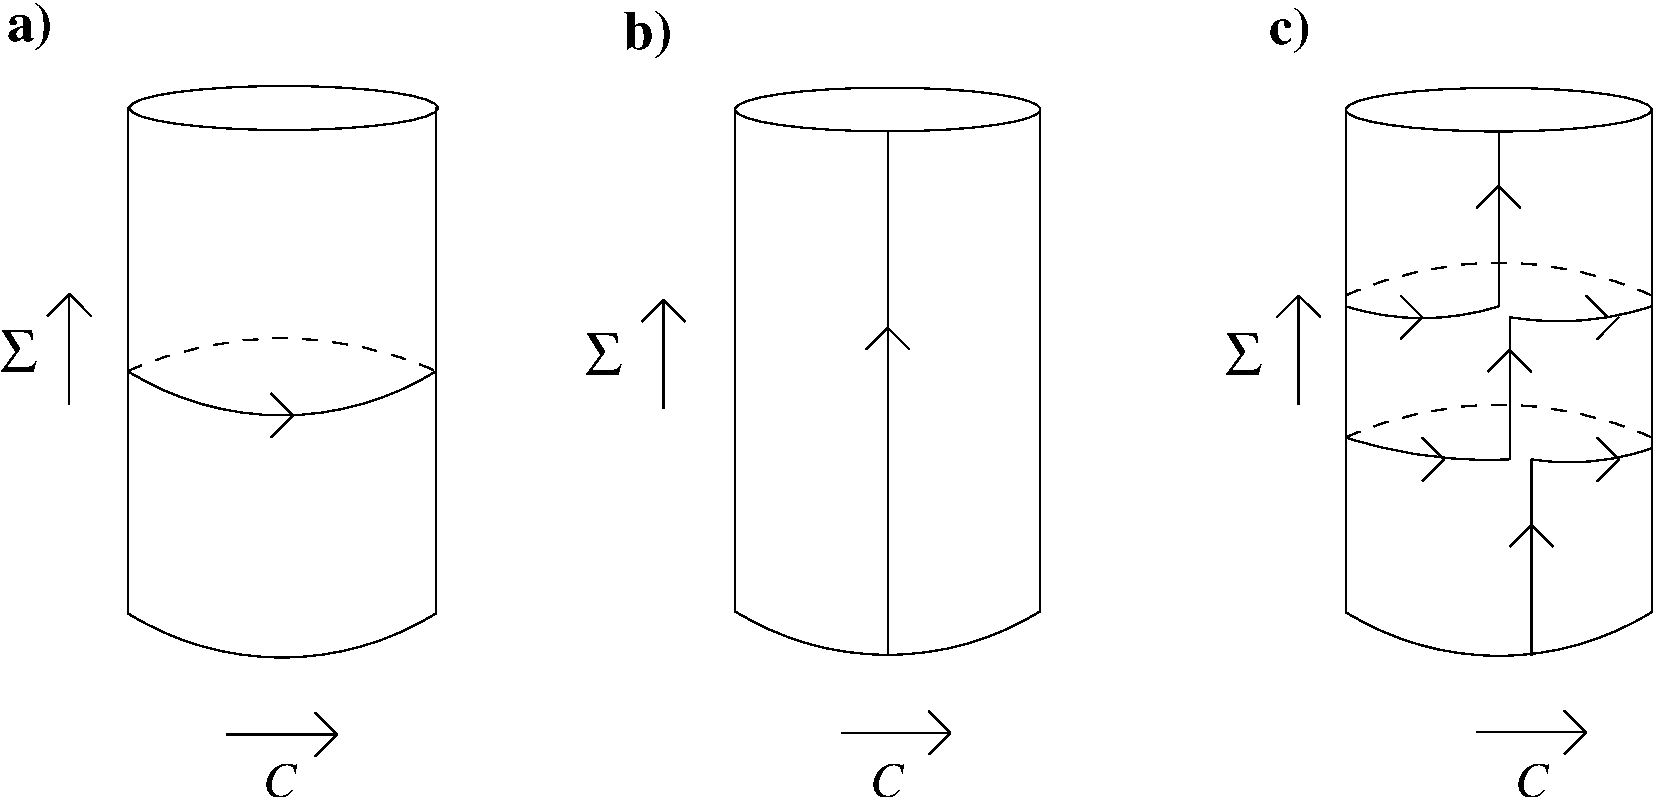
\includegraphics[width=0.75\linewidth]{figures/gla4-1.png}
\caption{四维流形 $\Sigma\times C$ 的示意图，其中 $\Sigma$ 竖直延伸、$C$ 水平延伸。(a) 沿 $C$ 方向传播的 Wilson 线。(b) 沿 $\Sigma$ 方向传播的 Wilson 线。(c) 沿 $\Sigma$ 方向传播、但在两个时刻绕着 $C$ 中一维闭链走一圈的 Wilson 线。（原文 Fig.~4）}
\label{fig:namp-four}  % 原文 \ifig\namp 同名重复（§6 Fig.~4 与 §8 Fig.~11），此处改名以免冲突
\end{figure}
 可以区分出几种情形。一种情形（\namp(a)）是形如 ${{\cal
S}}=p\times {{\cal S}}'$ 的圈，其中 $p$ 是 $\Sigma$ 中的一点，${{\cal S}}'$ 是 $C$ 中的一个圈。显然，支撑在这种圈上的算子，在 $\Sigma$ 上的有效理论中看起来就只是一个点状的局部算子。所有普通的量子场论以及许多 TQFT 都有这样的局部算子，所以在这个例子中，圈算子经过紧化之后变成了 $\Sigma$ 上有效理论中相当普通的东西。

相反的情形（\namp(b)）是 ${{\cal S}}={{\cal S}}''\times q$，其中 ${{\cal S}}''$ 是 $\Sigma$ 中的一个圈，$q$ 是 $C$ 中的一点。此时圈算子在二维有效理论中仍然是圈算子。

一般情形当然是一条在 $\Sigma$ 与 $C$ 中都非平凡地延伸的曲线 ${{\cal S}}$。任何这样的曲线都同伦于一条先在 $\Sigma$ 中延伸、再在 $C$ 中延伸、再在 $\Sigma$ 中延伸……如此反复的曲线，如 \namp(c) 所示。设 $\bar {{\cal S}}$ 是 ${{\cal S}}$ 到 $\Sigma$ 的投影。则 ${{\cal S}}$ 上的圈算子在 $\Sigma$ 上的有效理论中约化为 $\bar {{\cal S}}$ 上的圈算子，并在 $\bar {{\cal S}}$ 的一些特定点上插入了局部算子，这些点正是 ${{\cal S}}$ 绕着 $C$ 延伸的那些点。我们马上会给出这种圈算子的另一种解释。

\begin{figure}[htbp]
\centering
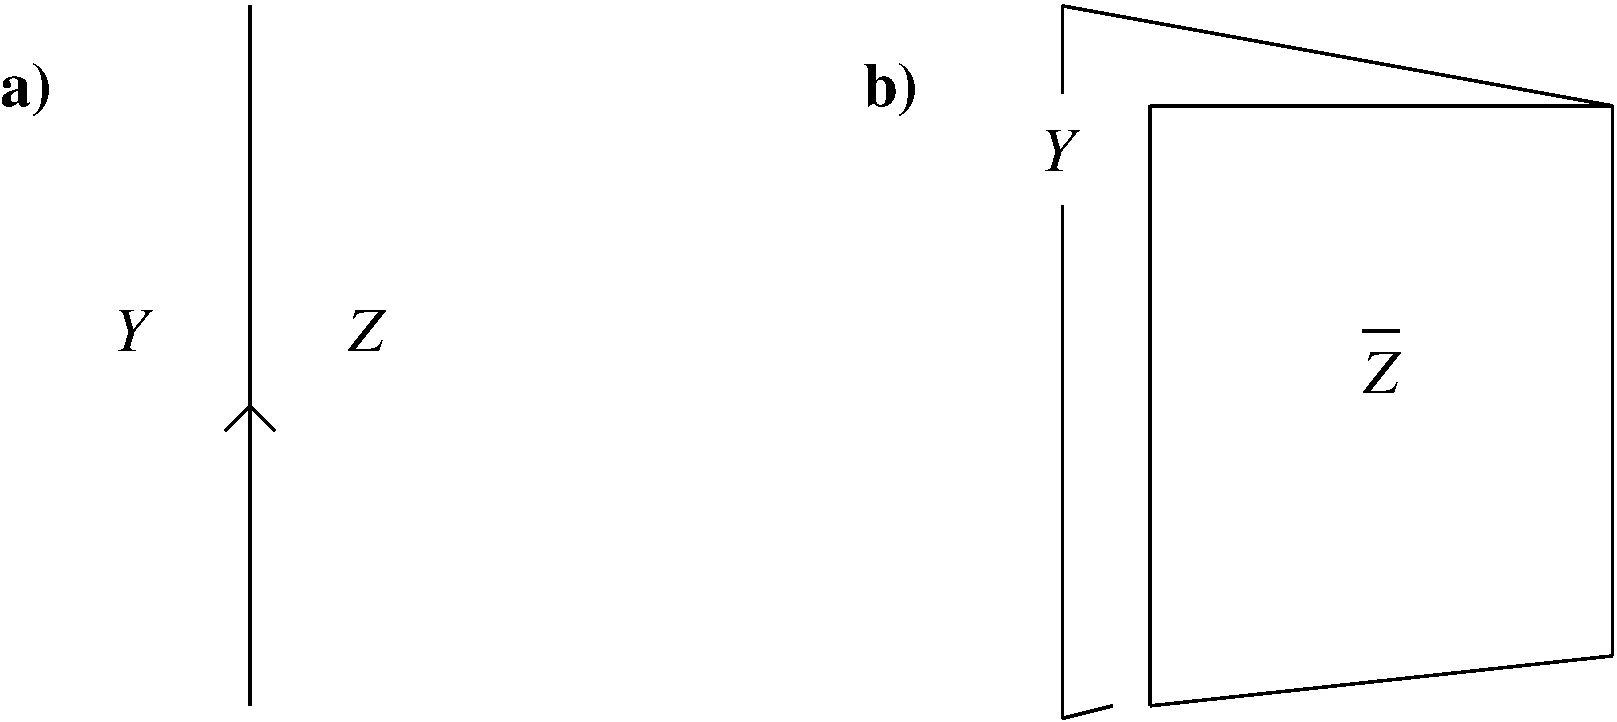
\includegraphics[width=0.75\linewidth]{figures/gla4-2.png}
\caption{(a) 一条线算子把平面分成两个区域，分别由理论 $Y$ 与 $Z$ 标记。(b) 同一图像折叠后的版本，用半平面上的理论 $Y\times \bar Z$ 来解释；其边界由 $(Y,Z)$-膜标记。（原文 Fig.~5）}
\label{fig:tonamp}
\end{figure}
 要点显然在于理解圈算子或线算子在二维中的含义。这里应当注意，一个二维流形局部地被一个一维流形分成两个不相交的区域。因此，一条圈算子或线算子可以产生长程效应；二维有效理论中的耦合常数可能在两侧不同。（Wilson 与 't Hooft 线算子如何能产生这种效应，将在第~\ref{sec:wilbranes}~节中讨论。）这一可能性已包含在 \tonamp(a) 中：那里画出的二维线算子把平面分成两个区域，分别由两个不同的理论 $Y$ 与 $Z$ 标记。

为了把这一情形放进更熟悉的框架，我们可以使用一个「折叠」（folding）技巧（例如见 \cite{ref93,ref94,ref95}）。代价是把区域 $Z$ 的定向反转，得到我们称之为理论 $\bar Z$ 的东西；这样我们就可以把 \tonamp(a)「折叠」，得到一幅类似的图，其中区域 $Y$ 与 $Z$ 位于同一侧，并终止于线算子所在的位置（\tonamp(b)）。

从抽象的观点来看，此时我们得到的是张量积理论 $Y\otimes \bar Z$ 中的一个边界条件。就本文的目的而言，所谓「膜」（brane），一般就是指量子场论中的一个局部边界条件。（换言之，我们的膜全都是 $D$-膜。）我们把乘积理论 $Y\otimes \bar Z$ 中的膜称为 $(Y,Z)$-膜。于是线算子在二维中约化为一个 $(Y,Z)$-膜。

现在我们也能够更好地理解 \namp(c)。此前我们把这一组态解释为带插入局部算子的线算子。折叠之后，二维有效理论被表述在带边界的黎曼面 $\Sigma$ 上，并且在边界上插入了局部算子。它们的存在正是膜物理的特征；一般而言，对任何膜，都存在一个局部算子空间，其元素可以插入到 $\Sigma$ 的由该膜标记的边界分支上。

\begin{figure}[htbp]
\centering
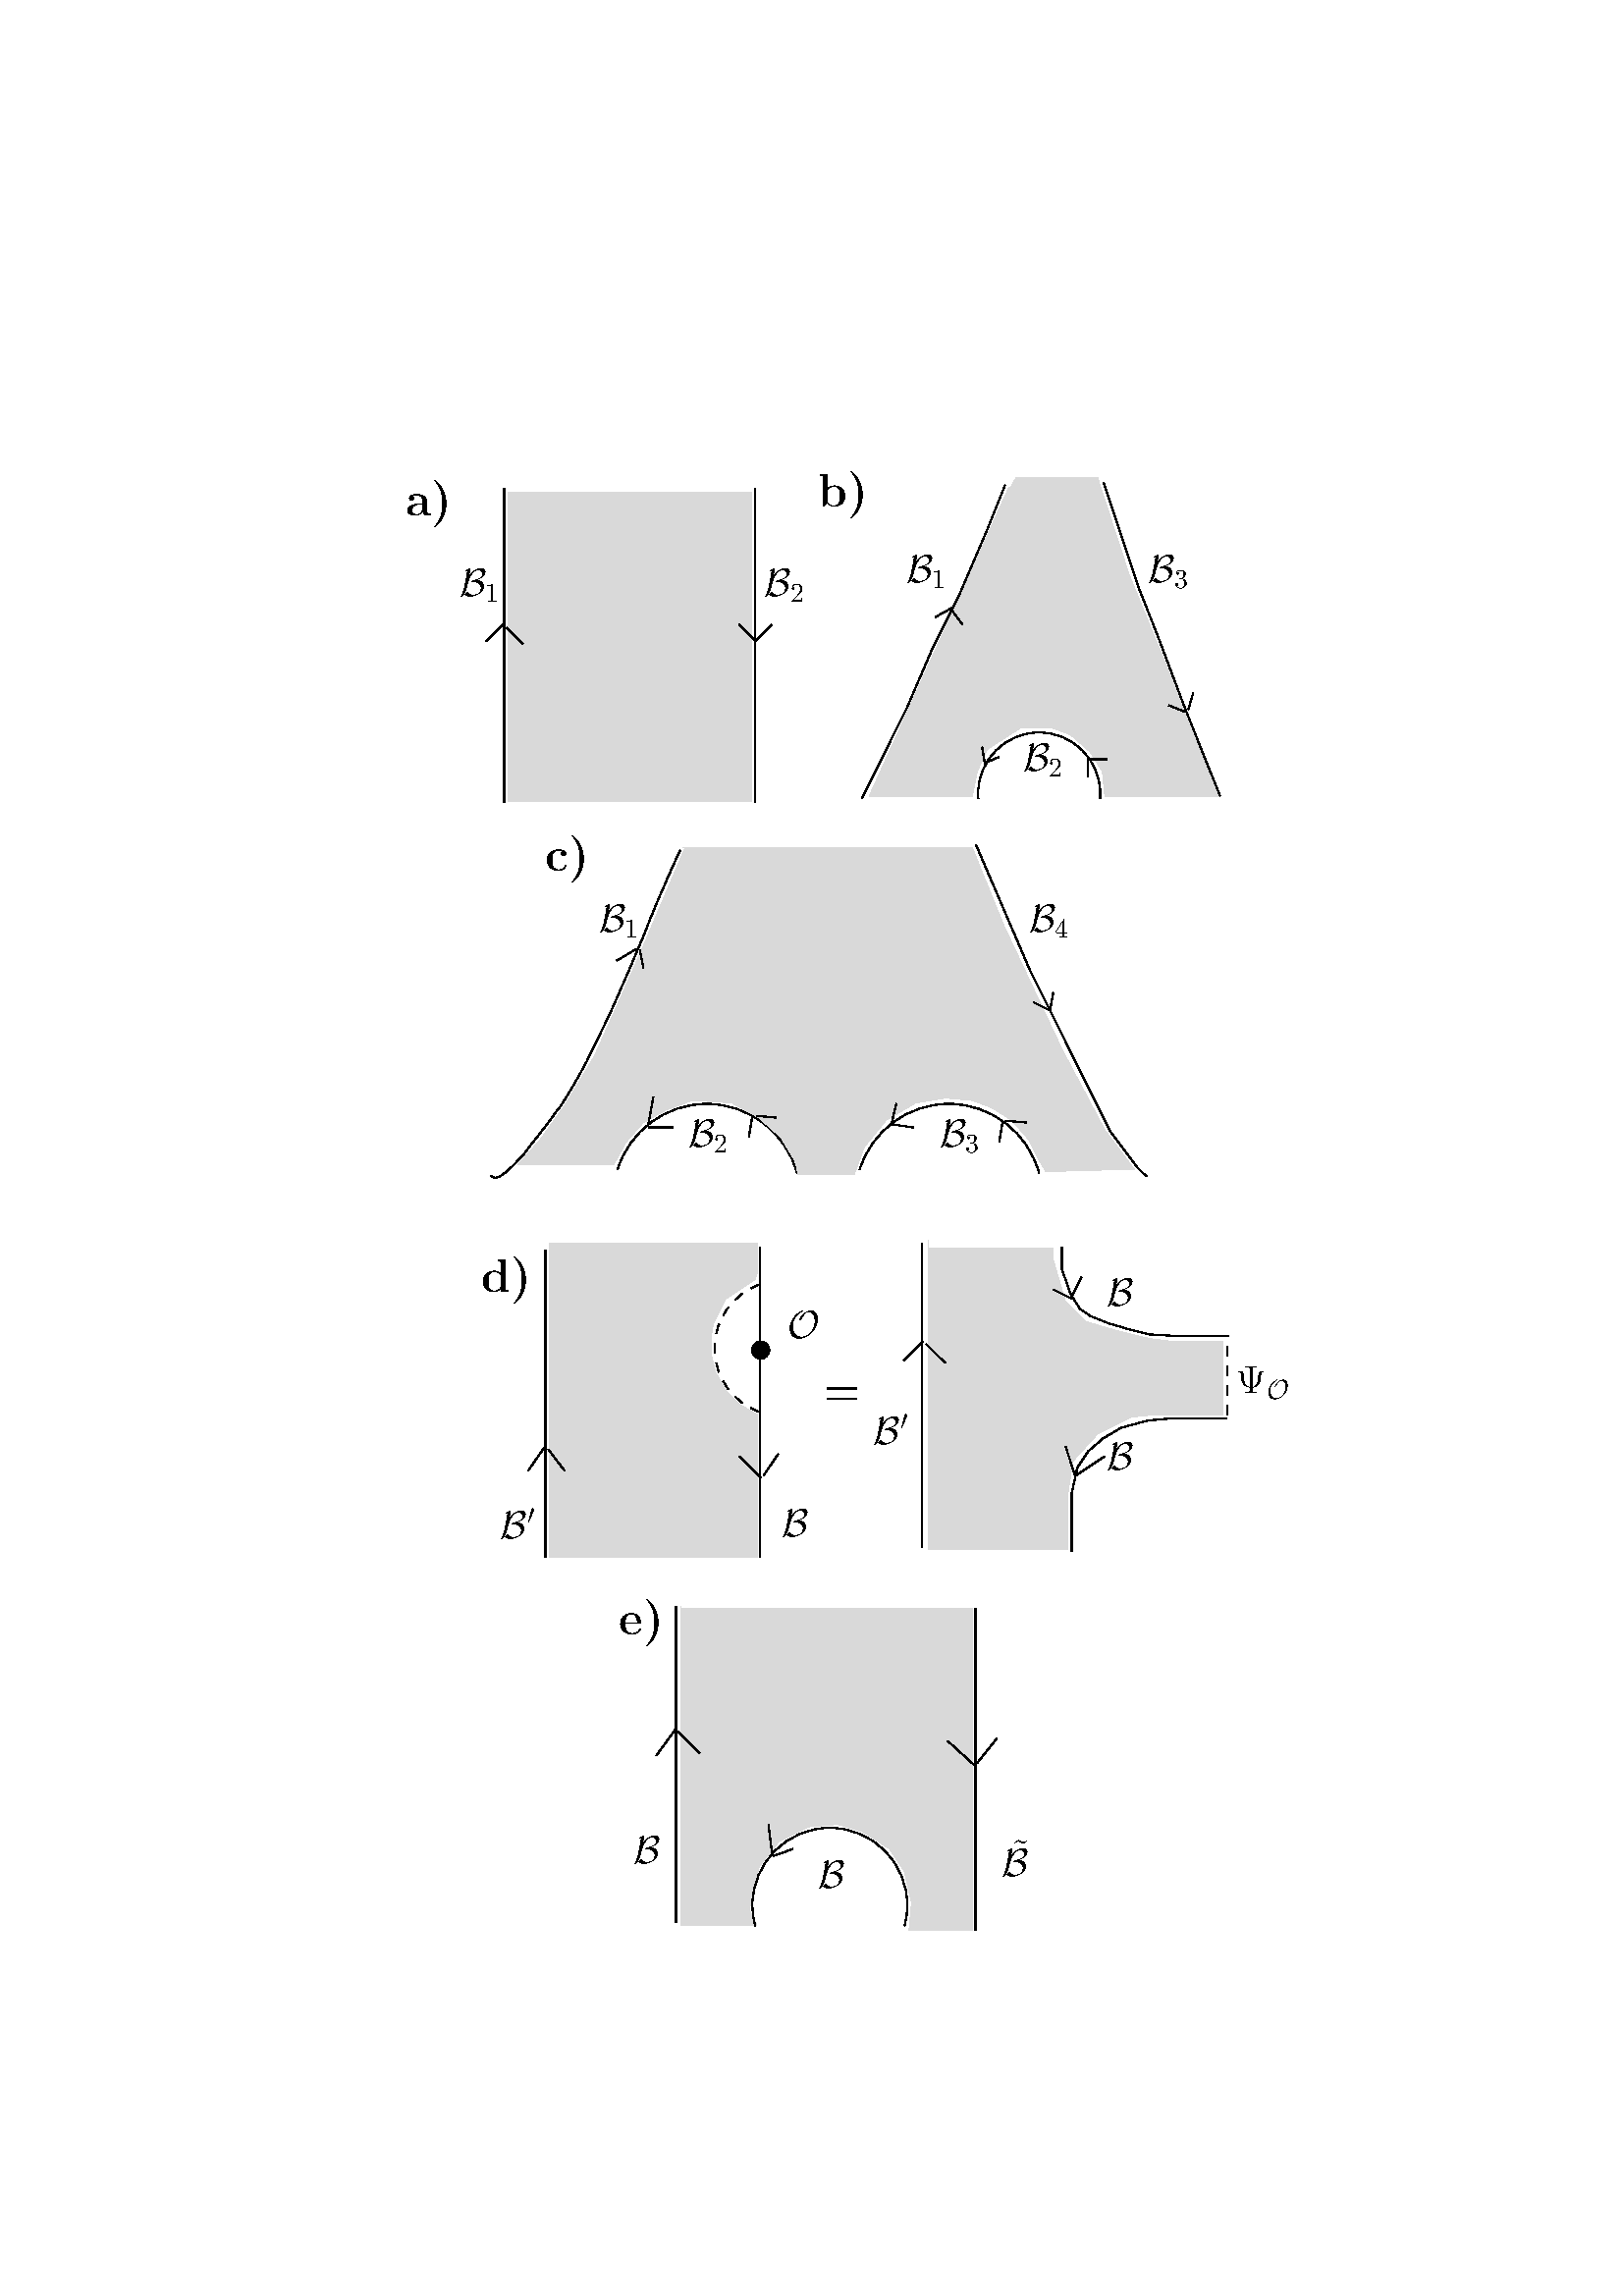
\includegraphics[width=0.75\linewidth]{figures/gla4-3.png}
\caption{(a) $({\cal B}_1,{\cal B}_2)$ 弦的空间。(b) 弦的粘接给出乘积 ${\cal H}_{{\cal B}_1,{\cal B}_2}\otimes {\cal H}_{{\cal B}_2,{\cal B}_3}\to {\cal H}_{{\cal B}_1,{\cal B}_3}$。(c) 由三条弦粘接得到的结合律关系。(d) 可插入由膜 ${\cal B}$ 标记的边界上的局部算子空间 ${\EUO}$ 与空间 ${\cal H}_{{\cal B},{\cal B}}$ 相同。为看出这一点，我们在 ${\EUO}$ 插入点附近的小区域（左图中未着色的区域）作路径积分，得到一个物理态 $\Psi_{\EUO}$，把它插入虚线处即可复现 ${\EUO}$ 的效应；所得图像可写成右图所示的形式。(e) 对每个 ${\cal B}$ 与 $\tilde{\cal B}$，空间 ${\cal H}_{{\cal B},\tilde{\cal B}}$ 是代数 ${\cal H}_{{\cal B},{\cal B}}$ 的一个模。（原文 Fig.~6）}
\label{fig:dunamp}
\end{figure}

 让我们回忆如何刻画这样的局部算子。这也有助于回忆关于膜的几个基本事实。对每个二维量子场论 $X$ 以及每一对膜 ${\cal B}_1$ 与 ${\cal B}_2$，都可以定义一个向量空间 ${\cal H}_{{\cal
B}_1,{\cal B}_2}$，即 $({\cal B}_1,{\cal B}_2)$ 弦的空间。在酉量子场论中，这些空间是 Hilbert 空间；即便没有酉性，${\cal H}_{{\cal B}_1,{\cal B}_2}$ 也对偶于 ${\cal H}_{{\cal B}_2,{\cal B}_1}$。${\cal H}_{{\cal
B}_1,{\cal B}_2}$ 的定义方式是：在 $\Sigma=\Bbb{R}\times I$ 上量子化理论 $X$，其中 $I$ 是单位区间，其两端分别由 ${\cal B}_1$ 与 ${\cal B}_2$ 标记（\dunamp(a)）。${\cal H}_{{\cal B}_1,{\cal B}_2}$ 也称为该理论在 $I$ 两端给定边界条件下的物理态空间。

而在拓扑场论中，对任意膜 ${\cal
B}_1,{\cal B}_2,$ 与 $ {\cal B}_3$，都有自然映射 ${\cal H}_{{\cal
B}_1,{\cal B}_2}\otimes {\cal H}_{{\cal B}_2,{\cal B}_3}\to {\cal
H}_{{\cal B}_1,{\cal B}_3}$，它们由把黎曼面粘接起来定义（\dunamp(b)）。（在没有拓扑不变性的二维量子场论中，必须把度规或曲面的共形结构考虑进去，其结果是一个类似的讨论会导出算子乘积展开。）这些映射满足显然的结合律关系，即当三条弦粘接时（\dunamp(c)），不必说清哪两条先粘接。特别地，把所有膜 ${\cal B}_i$ 都取为 ${\cal B}$，我们发现 ${\cal H}_{{\cal B},{\cal B}}$ 总具有结合代数的自然结构。

事实上，在 TQFT 中，可插入由膜 ${\cal B}$ 标记的边界上的局部算子空间 ${\EUO}$ 与 ${\cal H}_{{\cal B},{\cal B}}$ 相同，因为（\dunamp(d)）在这样的 ${\EUO}$ 附近施加一次「切割」操作，就会显示出 ${\cal H}_{{\cal B},{\cal B}}$ 的一个元素。由类似的推理（\dunamp(e)），我们发现，对任意 ${\cal B}$ 与 $ \tilde{\cal
B}$，${\cal H}_{{\cal B}, \tilde{\cal B}}$ 总具有左 ${\cal H}_{{\cal B},{\cal B}}$-模的自然结构。同样，它具有右 ${\cal H}_{\tilde
{\cal B},\tilde{\cal B}}$ 模的自然结构。事实上，${\cal H}_{{\cal B},
\tilde{\cal B}}$ 是一个 $({\cal H}_{{\cal B},{\cal B}},{\cal
H}_{\tilde{\cal B},\tilde{\cal B}})$ 双模。这只不过是说，可以用 ${\cal H}_{{\cal B},{\cal B}}$ 在左边贴一条弦来作用，也可以用 ${\cal H}_{\tilde{\cal B},\tilde{\cal
B}}$ 在右边贴一条弦来作用，而且这两个作用交换。

\begin{yizhu}[易错点]
圈算子约化到 $\Sigma$ 上并不总是圈算子。按其在 $C$ 与 $\Sigma$ 中走向的不同要分三类：（a）$p\times{{\cal S}}'$ 约化为 $\Sigma$ 上的点状局部算子；（b）${{\cal S}}''\times q$ 仍是 $\Sigma$ 上的圈算子；（c）一般曲线约化为 $\bar{{\cal S}}$ 上的圈算子加若干特定点处的局部算子插入。把（a）也当成「圈算子」留在二维理论里是最常见的误读。
\end{yizhu}

\begin{yizhu}[物理图像]
折叠技巧（folding trick）的要点：线算子把平面分成标记为 $Y$ 与 $Z$ 的两个区域；把 $Z$ 反定向、改称 $\bar Z$ 并把图折过来，就得到 $Y\otimes\bar Z$ 张量积理论中位于半平面上的一个边界条件，即 $(Y,Z)$-膜。于是「线算子」被翻译成「膜（=局部边界条件）」。这一步也是后文把四维线算子变成二维膜、进而用膜范畴讨论线算子的起点。
\end{yizhu}

\begin{yizhu}[易错点]
${\cal H}_{{\cal B}_1,{\cal B}_2}$ 是量子化所得的态空间，不是某个几何上预先给定的向量空间：它由在 $\Sigma=\Bbb{R}\times I$ 上量子化、两端分别贴膜 ${\cal B}_1$ 与 ${\cal B}_2$ 定义，并要求 $I$ 是单位区间。粘接黎曼面给出乘积 ${\cal H}_{{\cal B}_1,{\cal B}_2}\otimes{\cal H}_{{\cal B}_2,{\cal B}_3}\to{\cal H}_{{\cal B}_1,{\cal B}_3}$，其结合律使 ${\cal H}_{{\cal B},{\cal B}}$ 成为结合代数；对一般的 ${\cal B},\tilde{\cal B}$，${\cal H}_{{\cal B},\tilde{\cal B}}$ 是左 ${\cal H}_{{\cal B},{\cal B}}$-模、右 ${\cal H}_{\tilde{\cal B},\tilde{\cal B}}$-模，即双模，两种作用交换。
\end{yizhu}

\begin{yizhu}[含糊点拨]
原文特意声明「by a brane, in general, we simply mean a local boundary condition in a quantum field theory」并补一句「our branes are all $D$-branes」。按 GLOSSARY 的定译，本文一律译作「膜」而不加 D-；但读者应记住这里的膜就是局部边界条件（特殊的 D-膜），并非任意延展对象。
\end{yizhu}

\begin{yizhu}[物理图像]
图 6(d) 的「切割」论证是 TQFT 中「局部算子 = 边界态」的标准等价：在算子 ${\EUO}$ 的插入点周围的小区域里作路径积分，得到边界上的一个物理态 $\Psi_{\EUO}$，把这个态插回虚线处就复现了 ${\EUO}$ 的效应。正因如此，${\EUO}$ 的空间才等于 ${\cal H}_{{\cal B},{\cal B}}$；而在非拓扑的二维量子场论中，对应的构造会给出算子乘积展开。
\end{yizhu}

\begin{yizhu}[原文疑误]
原文第 136 行作 「can be inserted on a a boundary labeled by ...」，其中「a a」是重复冠词，系底本笔误（应为单个 a）。译文按单数不定冠词处理，语义不受影响。
\end{yizhu}

%% ============================================================
%% 分片 18：原文第 6 节「Loop and Line Operators」（原文 glshort.tex 起于第 4483 行）
%% 由 tools/harvmac2tex.py 从 arXiv 源码（hep-th/0604151v3）自动生成。
%% 只译英文散文；公式、编号、\label、\cite 一律不改。
%% ============================================================

\subsection{边界附近的线算子}

\label{sec:lineop}

几何 Langlands 纲领围绕的是这样一种情形：$\Sigma$ 有边界，而线算子平行于该边界。

\begin{figure}[htbp]
\centering
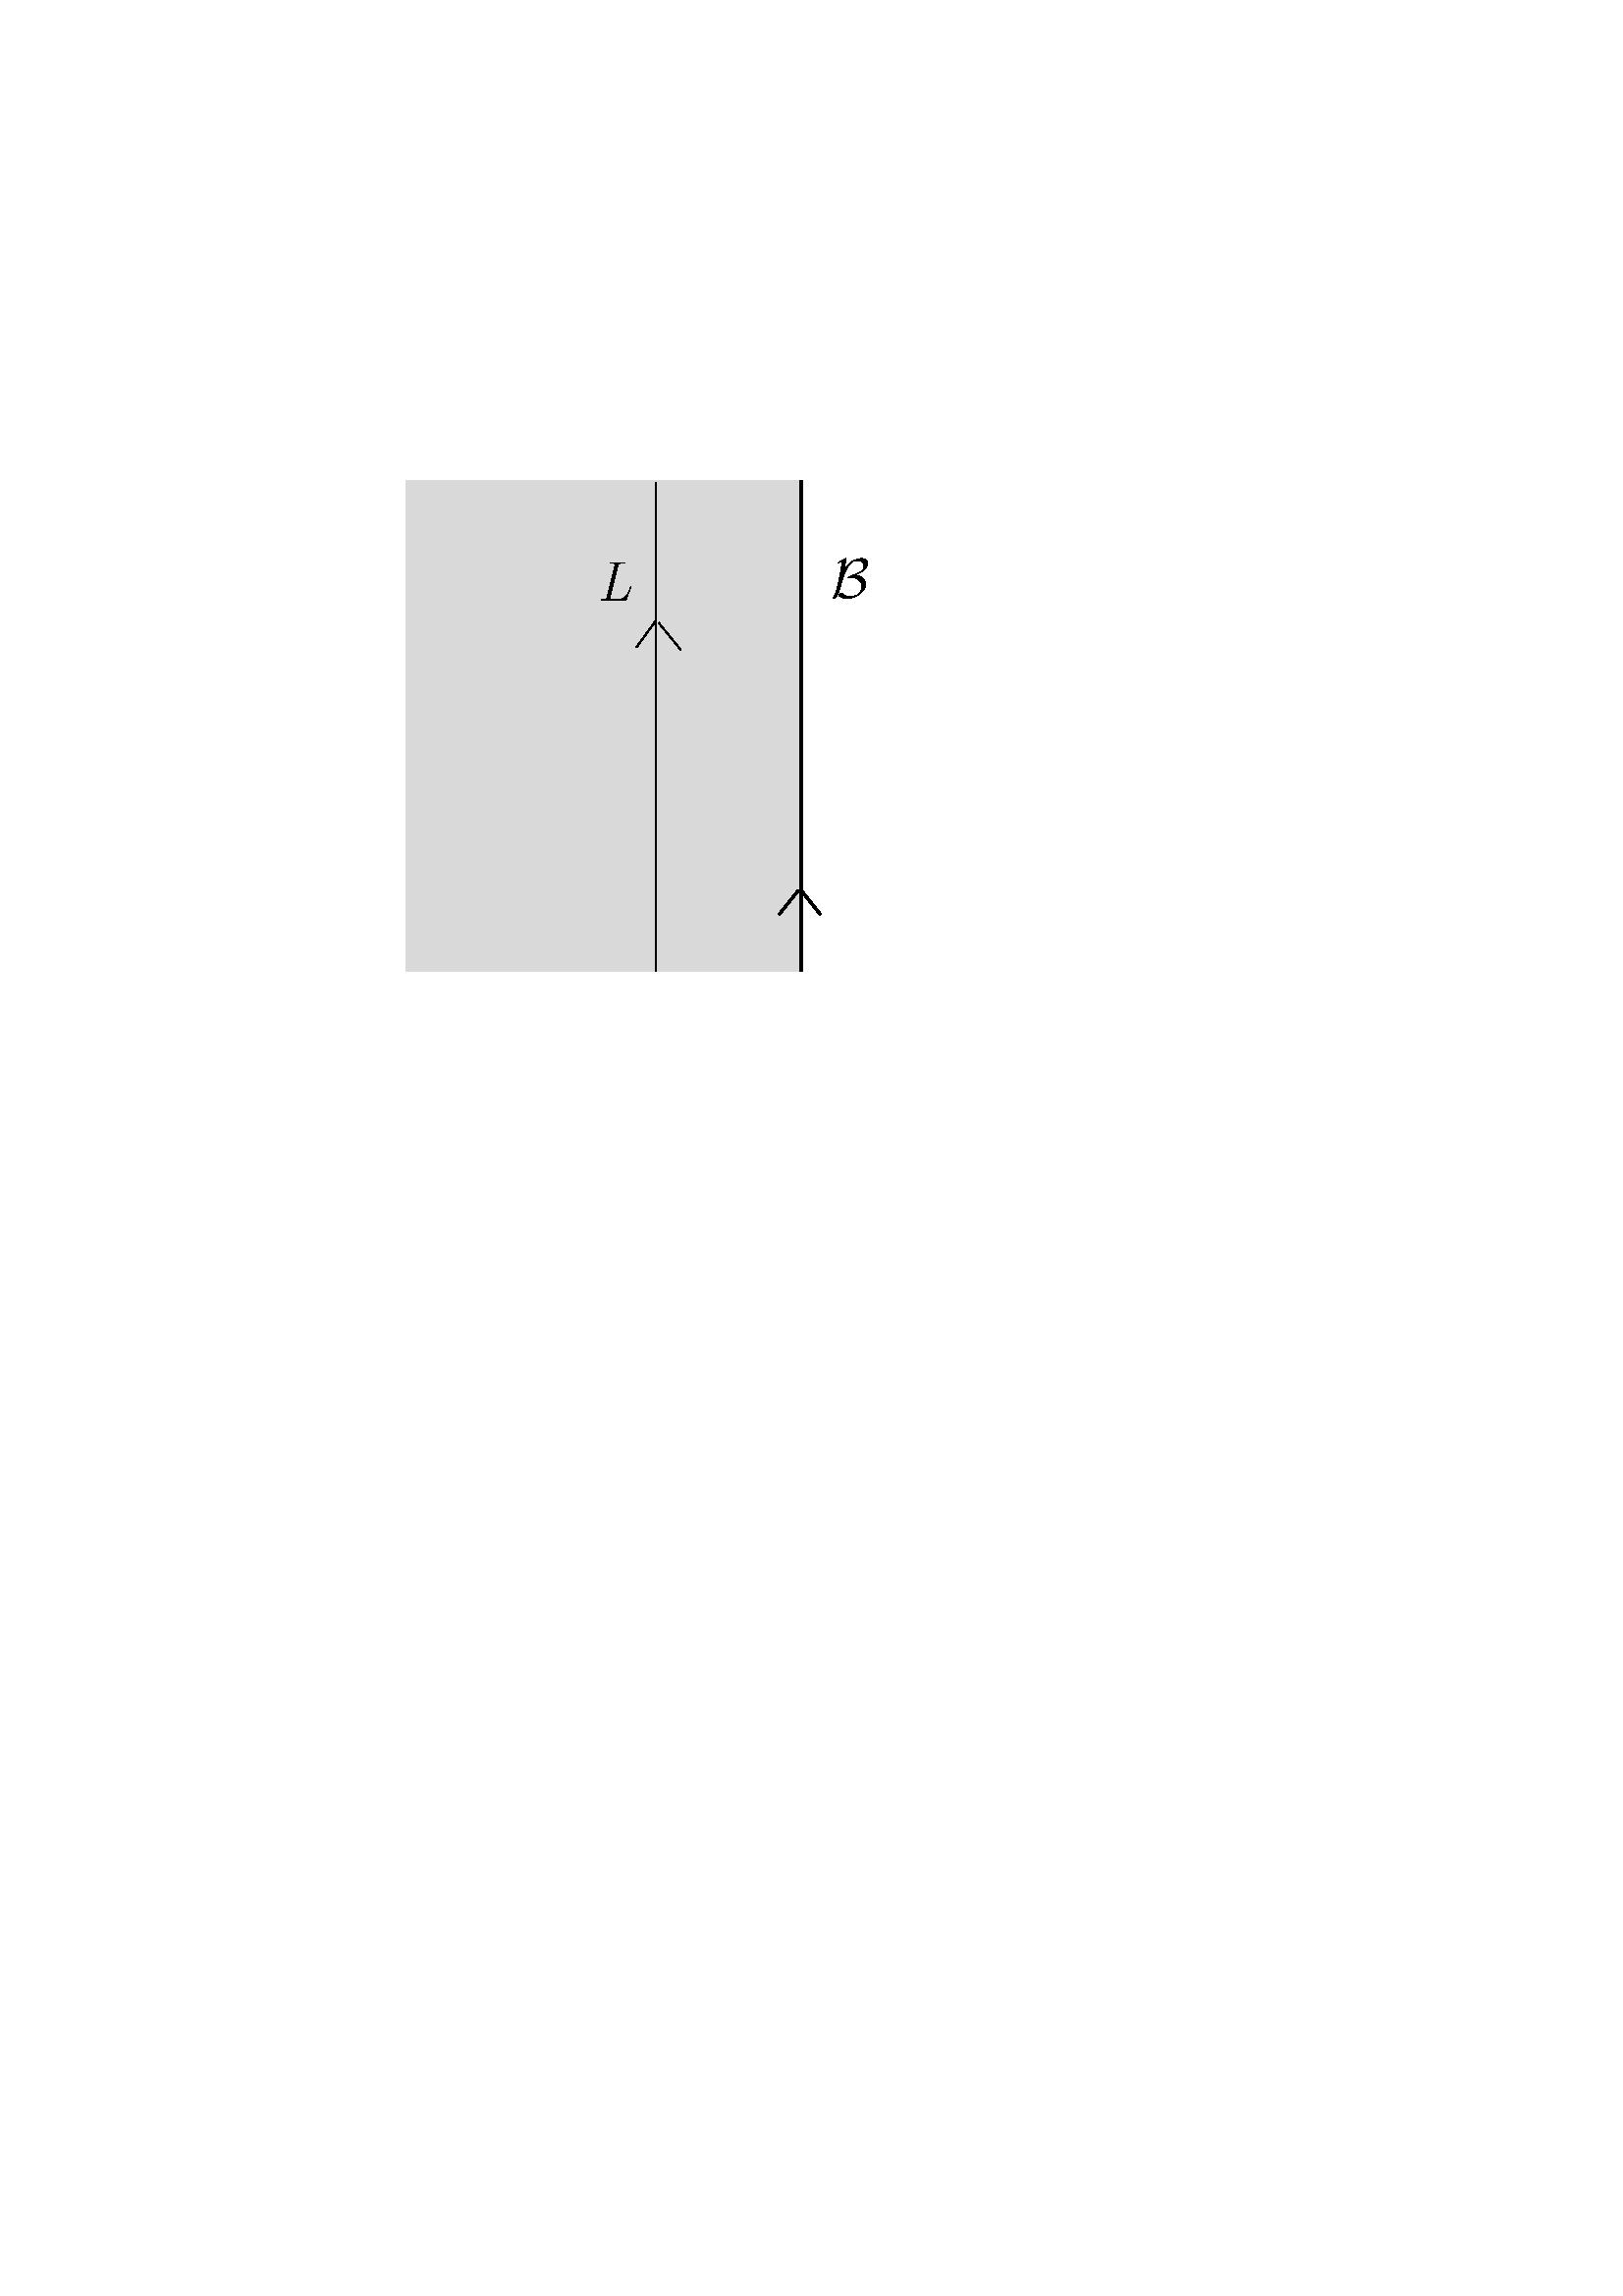
\includegraphics[width=0.75\linewidth]{figures/gla4-4.png}
\caption{带边界的黎曼面，其边界由膜 ${\cal B}$ 标记，另有一条平行于边界的线算子 $L$。（原文 Fig.~7）}
\label{fig:trinamp}
\end{figure}

 在带边界的黎曼面 $\Sigma$ 上定义量子场论需要选定一个边界条件——也就是选定一个膜，我们把它记作 ${\cal B}$。在 \trinamp 中，我们画出一个带边界的黎曼面 $\Sigma$ 以及一条平行于边界的线 $L$。该边界已由膜 ${\cal B}$ 标记，它规定了该边界处的边界条件。线算子 $\EUX$ 支撑在 $L$ 上。$\EUX$ 可以是 Wilson 算子、't Hooft 算子或混合 Wilson-'t Hooft 算子。

{}从宏观观点看，$\EUX$ 与 ${\cal B}$ 只不过合并成一个有效边界条件 ${\cal B}'$。人们可以把 ${\cal B}'$ 刻画为：由于 ${\cal B}$ 与 $\EUX$ 的联合效应，在大距离处看到的那个有效边界条件。或者也可以简单地取 $L$ 趋近边界的极限，让 ${\cal B}'$ 成为所得的极限边界条件。

无论用哪种方式，我们都把由 $\EUX$ 作用于旧膜所产生的新膜记作 ${\cal B}'=\EUX {\cal B}$。这样，我们就把线算子看作作用在边界条件上、产生新边界条件的东西。

\begin{figure}[htbp]
\centering
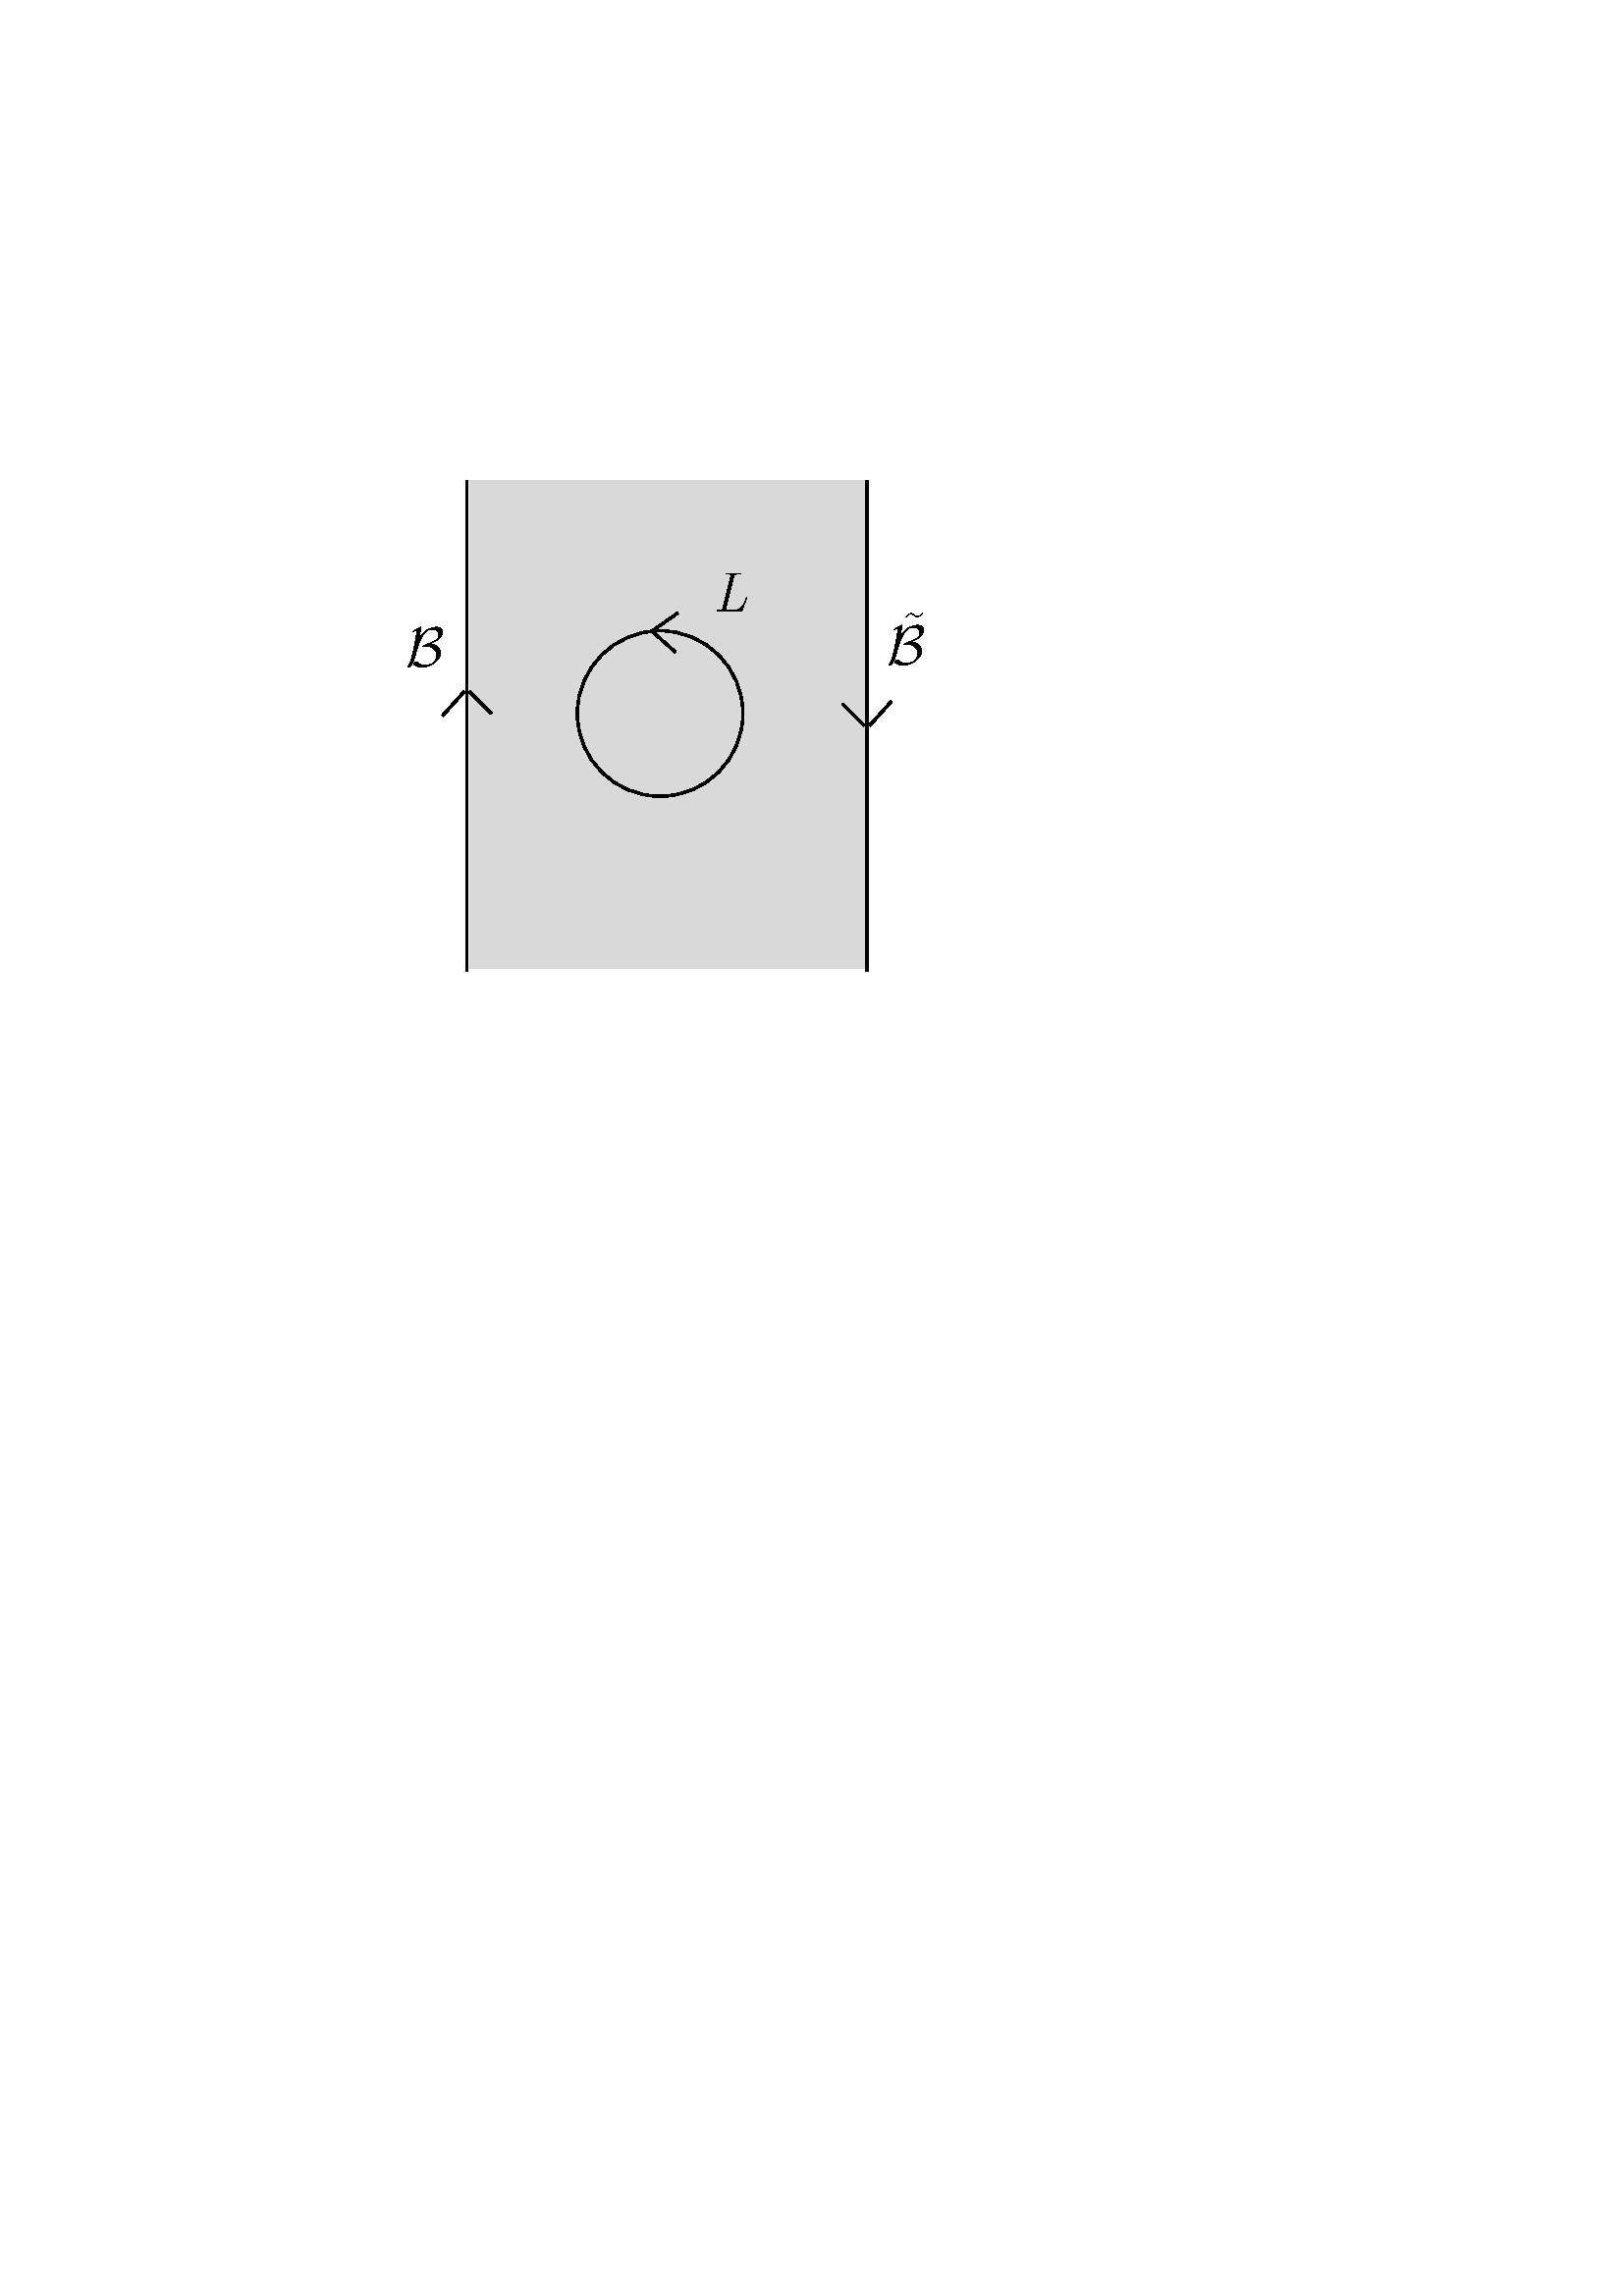
\includegraphics[width=0.75\linewidth]{figures/gla4-5.png}
\caption{圈算子作为普通算子作用在空间 ${\cal H}_{\cal B,\tilde{\cal B}}$ 上。（原文 Fig.~8）}
\label{fig:quadramp}
\end{figure}
 这是一种比算子通常作用于向量空间更为抽象的作用。如我们在上面所见，要得到与 ${\cal B}$ 相联系、可供某个算子作用的向量空间 ${\cal H}_{{\cal B},\tilde
{\cal B}}$，我们需要一对膜 ${\cal B}$ 与 $\tilde {\cal B}$。当然，我们也可以就取 $\tilde {\cal B}={\cal B}$。但即便构造出物理态空间 ${\cal H}_{{\cal B},\tilde {\cal B}}$，真正作用在该空间上的其实是一个{\it 圈}算子——它定域于时间——其作用方式是对 \quadramp 的图景作量子化。而沿时间方向延伸的开线算子（如 \trinamp 中那样）则是另一回事：它是量子化时必须纳入的数据的一部分，只有纳入它才能得到正确的物理态空间。

如果我们{\it 确实}有一个向量空间 ${\cal H}$ 和一个算子 ${\EUO}:{\cal H}\to {\cal H}$，我们就可以寻找 ${\EUO}$ 的本征向量 $\psi\in
{\cal H}$：
% 式 (6.21)
\setcounter{equation}{20}
\begin{equation}\label{eq:reot}
{\EUO}\psi=\lambda\psi.
\end{equation}
 这里 $\lambda$ 是一个普通的复数。

在我们的问题中，不是作用于 Hilbert 空间向量的算子，而是一个更奇异的、经由 ${\cal B}\to {\cal B}'=\EUX {\cal B}$ 作用于理论上的算子。在这种情况下，普通的复本征值没有意义。取而代之，起「本征值」作用的是一个向量空间 $V$。

对每个膜 ${\cal B}$ 与向量空间 $V$，都可定义一个新膜 ${\cal B}\otimes V$。刻画 ${\cal B}\otimes V$ 的一种抽象方式是：对任意膜 $\tilde {\cal B}$，Hilbert 空间 ${\cal H}_{\tilde {\cal B},{\cal B}\otimes V}$ 等于 ${\cal H}_{\tilde {\cal B}, {\cal B}}\otimes V$。

对于由几何构造出的膜，我们可以说得更具体。当理论 $X$ 是靶空间为 $\hat X$ 的二维 sigma 模型时，可以从一个向量丛 ${\cal W}\to \hat X$（或更一般的、可能支撑在子流形上的层）构造出膜。${\cal
W}$ 称为 Chan-Paton 丛。把这样的膜与固定的向量空间 $V$ 作张量积，只不过是把 ${\cal W}$ 换成 ${\cal
W}\otimes V$。当 ${\cal W}$ 换成更一般的层时，这一运算毫无困难地推广。

若把 $V$ 等同于某个 $\Bbb{C}^k$，则把 Chan-Paton 丛与 $V$ 作张量积相当于取原膜的 $k$ 个拷贝。所以 ${\cal B}$ 是 $\EUX$ 的特征膜（eigenbrane）意味着 $\EUX{\cal B}$ 同构于 ${\cal B}$ 的 $k$ 个拷贝的直和。然而，远为更好的做法是把「本征值」想成一个向量空间 $V$，而不只是它的整数维数 $k$，因为 $V$ 实际上可以作为某个参数空间上向量丛的纤维而随附加参数变化。

建立了把膜与向量空间作张量积的概念之后，我们现在就可以定义特征膜的概念。若存在向量空间 $V$ 使得
% 式 (6.22)
\setcounter{equation}{21}
\begin{equation}\label{eq:intico}
\EUX {\cal B}={\cal B}\otimes V,
\end{equation}
 则称膜 ${\cal B}$ 是线算子 $\EUX$ 的特征膜。这一概念对应于 Beilinson 与 Drinfeld 在几何 Langlands 纲领中定义的「特征层」（eigensheaf）概念 \cite{ref5}。

\begin{figure}[htbp]
\centering
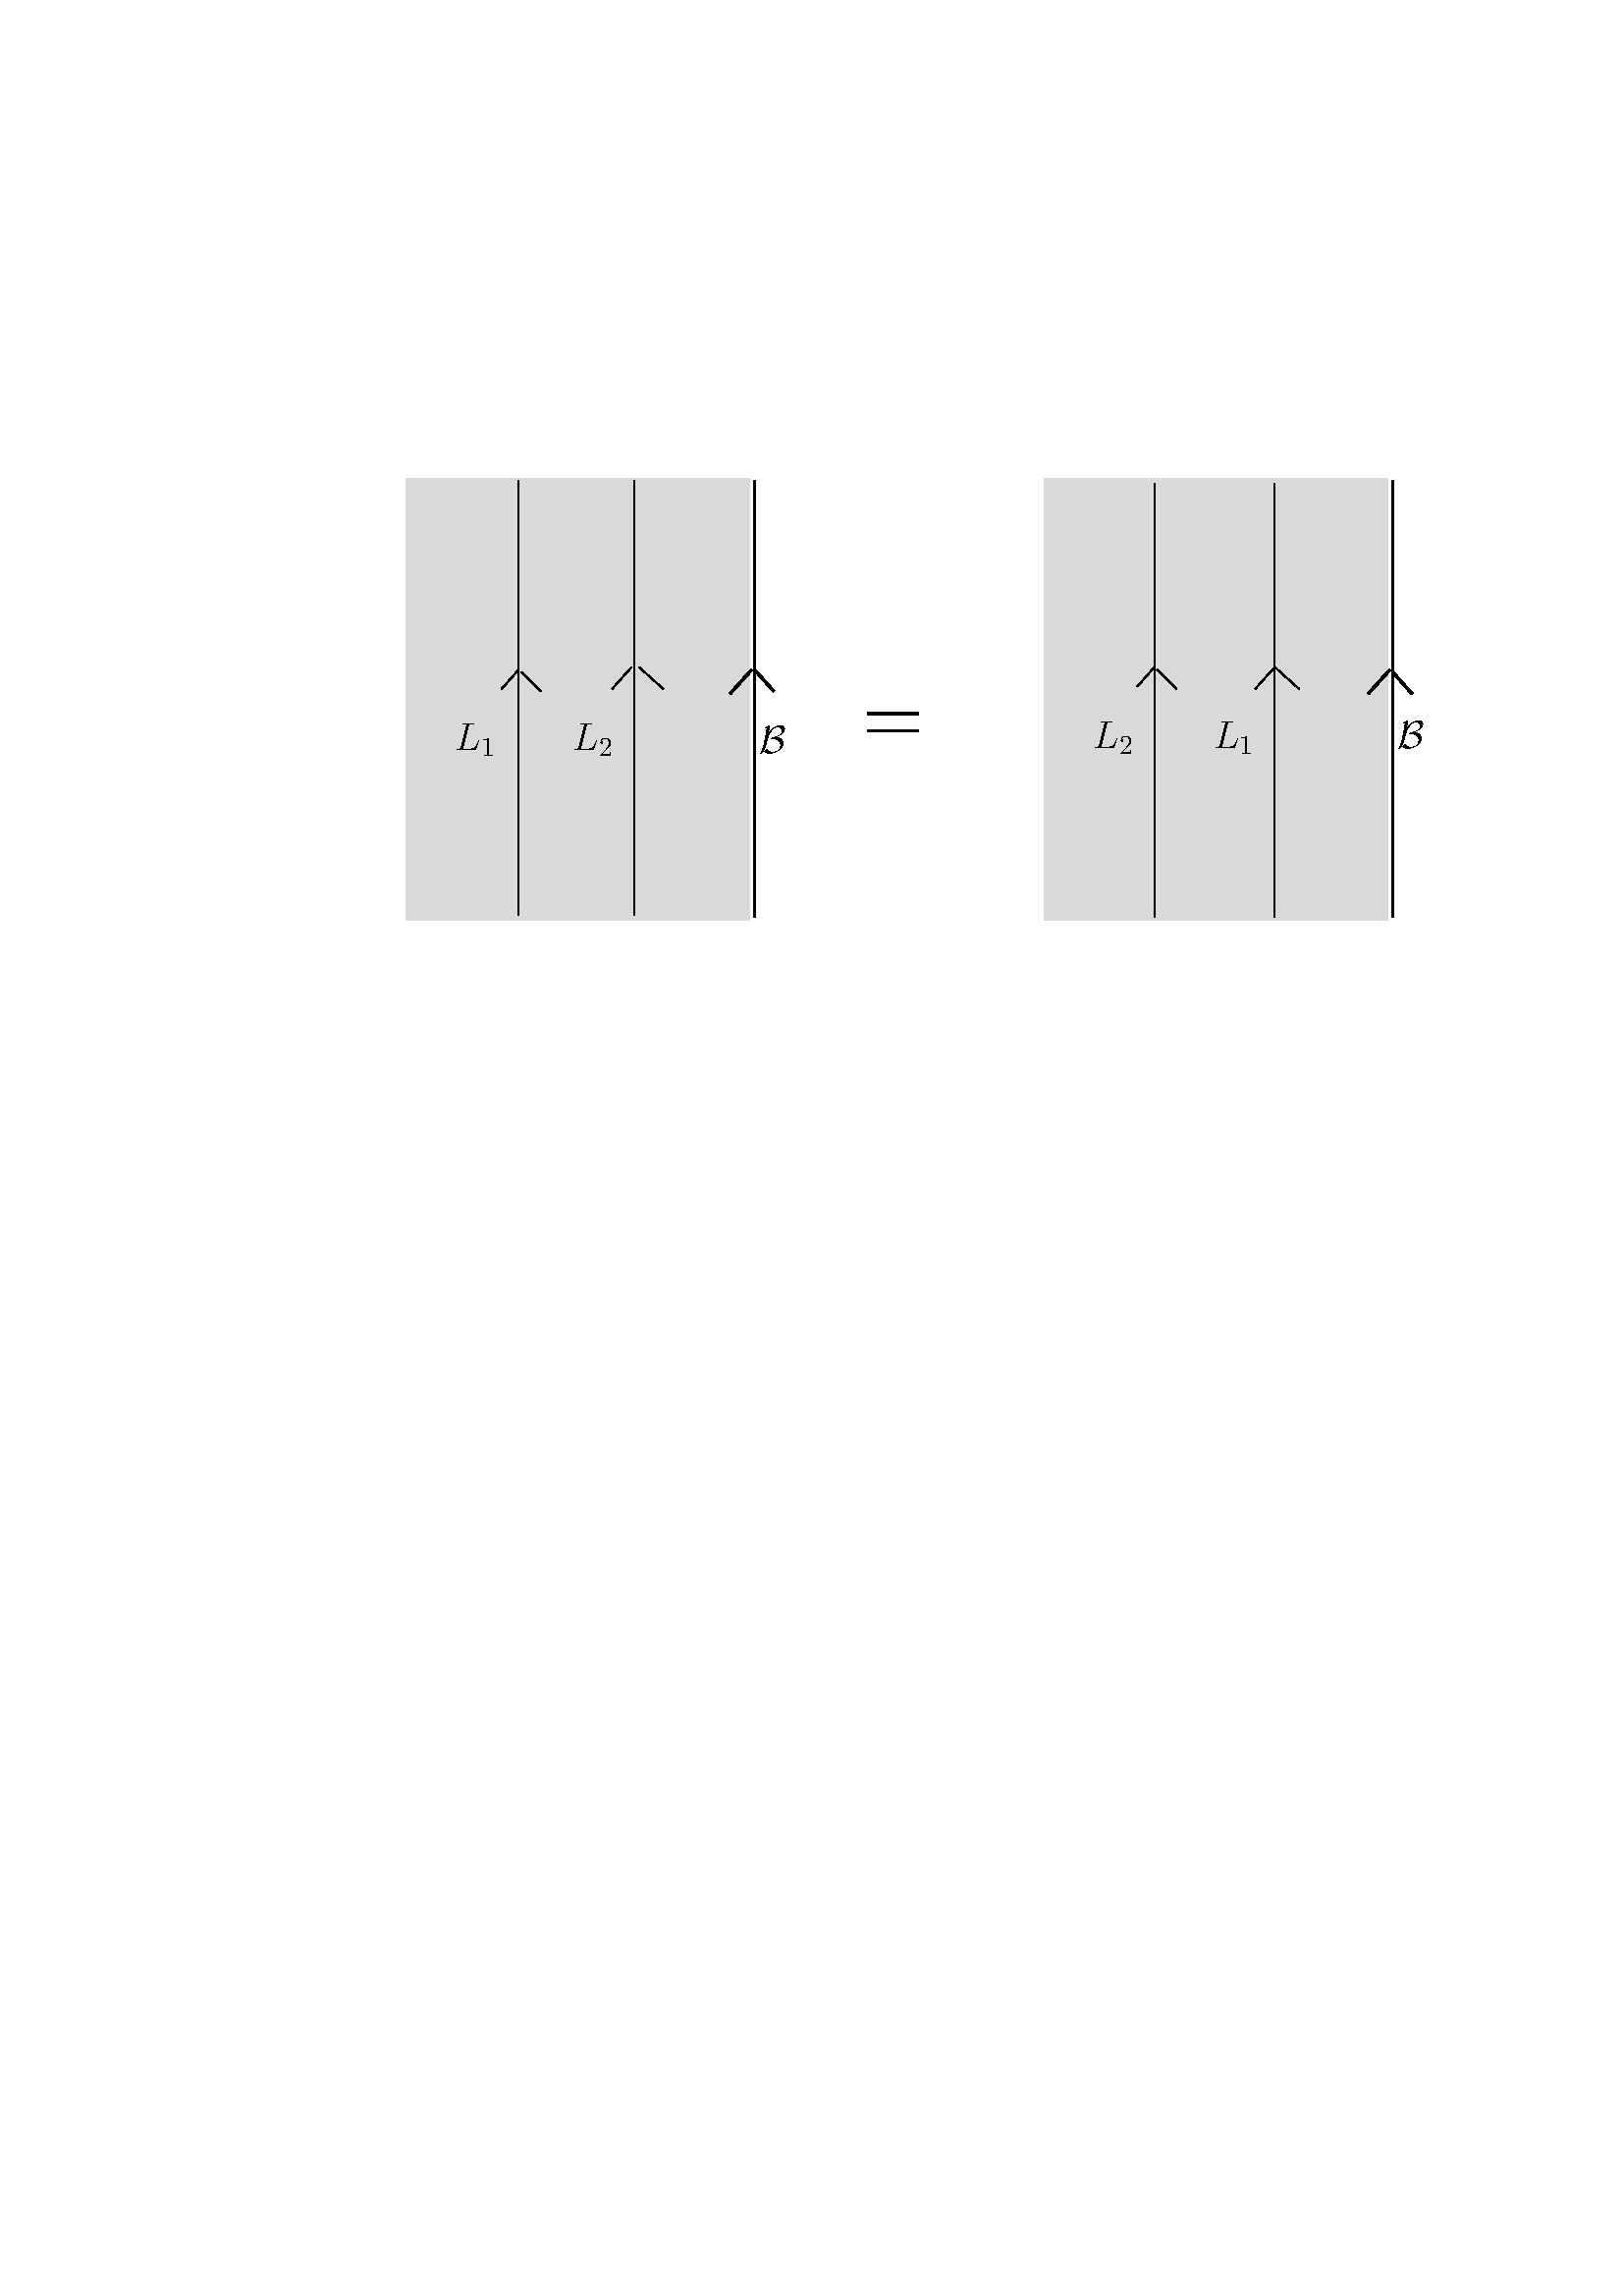
\includegraphics[width=0.75\linewidth]{figures/gla4-6.png}
\caption{若两条线算子 $L_1$ 与 $L_2$ 能彼此穿过而不产生奇异性，则称它们交换。在拓扑场论中，这不过是说此处所画的两幅图可以视为等价。（原文 Fig.~9）}
\label{fig:quintamp}
\end{figure}
 若 $\EUX_1$ 与 $\EUX_2$ 是支撑在平行线 $L_1$ 与 $L_2$ 上的两个线算子，且对所有 ${\cal B}$ 都有
% 式 (6.23)
\setcounter{equation}{22}
\begin{equation}\label{eq:pintico}
\EUX_1\EUX_2{\cal B}=\EUX_2\EUX_1{\cal B}.
\end{equation}
 我们就说它们交换。这一陈述可以用一幅方便的图来说明：它意味着线 $L_1$ 与 $L_2$ 可以彼此穿过而不产生任何不连续性（\quintamp）。正如 Hilbert 空间上的普通算子那样，若两个线算子在此意义下交换，它们就可能具有共同特征膜，即满足下式的膜 ${\cal B}$：
% [WARN] 公式 \eqn\eqref{eq:pintico} 无编号或重复
\begin{equation*}
\tag*{(6.24)}
\begin{aligned}\EUX_1{\cal B}& = {\cal B}\otimes V_1\\
\EUX_2{\cal B}& = {\cal B}\otimes V_2.\\\end{aligned}
\end{equation*}
 更一般地，任意一族交换的线算子都可以有共同特征膜。

\par\medskip{\it 来自四维的线算子}

在我们的问题中，我们关心的是把四维 TQFT 在黎曼面 $C$ 上约化所得的二维 TQFT。此外，我们的线算子全都来自四维的线算子。这就足以保证某些特殊行为。

首先，每个线算子 $\EUX$ 都可以对任意点 $p\in C$ 定义。为明确起见，我们把线算子写成 $\EUX_p$。若保持拓扑对称的膜 ${\cal B}$ 对某个 $p$ 是 $\EUX_p$ 的特征膜，它就必定对每个 $p$ 都是特征膜，因为 $p$ 本来就无关紧要。所以
% 式 (6.25)
\setcounter{equation}{24}
\begin{equation}\label{eq:hintico}
\EUX_p{\cal B}={\cal B}\otimes V_p
\end{equation}
 对某个 $V_p$ 成立。
这里，局部地说，向量空间 $V_p$ 必须与 $p$ 无关，因为 $p$ 无关紧要。但拓扑不变性容许一种可能：当 $p$ 在黎曼面 $C$ 上变化时，$V_p$ 可以有整体单值。所以这些 $V_p$ 是 $C$ 上某个平坦向量丛的纤维。

更明确地说，移动 $p$ 等价于改变 $C$ 上度规的一个特殊情形，而这会把底层作用量改变一个 BRST-平凡的项 $\{Q,\cdot\}$。这一事实使人能够为 $p\in C$ 的向量空间族 $V_p$ 找到一个平坦联络，从而局部地证明 $V_p$ 与 $p$ 无关。但这个平坦联络可以有非平凡的整体单值。

假设给定若干个都保持同一拓扑对称的圈算子 $\EUX_i$。例如，在 $\Psi=\infty$ 处，它们可以是与 $G$ 的表示 $R_i$ 相联系的 Wilson 算子；在 $\Psi=0$ 处，它们可以是与 $^L\negthinspace G$ 的表示 $^L\negthinspace R_i$ 相联系的 't Hooft 算子。无论如何，这些 $\EUX_i$ 都依赖于点 $p_i\in C$。由于我们可以自由地把点 $p_i$ 取为互不相同，我们就可以施行 \quintamp 中的交换——从二维观点看这可能是奇异的——而不遇到任何奇异性。（线算子在四维中并不相交，所以不可能出现奇异性。而且，由于 $C$ 是二维的，移动线算子时有足够的余地，使我们不会遇到沿 $C$ 局部出现的单值。\footnote{若 $L$ 与 $L'$ 是支撑在同一点 $p\in C$ 的两条线算子，要使它们在 $\Sigma\times C$ 中无奇异地彼此穿过，我们把它们分开到两个不同的点 $p,p'\in C$，其中 $p'$ 靠近 $p$。这可以在一个小开球 $U\subset C$ 中做到。对 $\Sigma=\Bbb{R}\times I$，静态线算子支撑在三维流形 $W=I\times C$ 中的点上，而把 $L$ 移过 $L'$ 的操作可以在子空间 $W'=I\times U$ 中完成。$W'$ 中不同点对构成的空间是单连通的，所以在这个局部模型中没有单值，也不存在如何把 $L$ 移过 $L'$ 的歧义。若 $C$ 是一维的，这一论证就不成立。}）因此，具有四维起源的拓扑线算子自动交换。

\par\medskip{\it 电特征膜与磁特征膜}

作为一个特例，$\Psi=\infty$ 处的拓扑 Wilson 算子交换。因此它们可以有共同特征膜。Wilson 线算子的共同特征膜称为电特征膜（electric eigenbrane）。

类似地，$\Psi=0$ 处的拓扑 't Hooft 算子交换，同样可以有共同特征膜。't Hooft 算子的共同特征膜称为磁特征膜（magnetic eigenbrane）。

$S$-变换 $S:\Psi\to -1/n_{\frak g}\Psi$ 把拓扑 Wilson 算子映为拓扑 't Hooft 算子，从而把电特征膜映为磁特征膜。

与任何一族来自四维的线算子的特征膜一样，电特征膜与磁特征膜自动与 $C$ 上的平坦向量丛相联系。这是几何 Langlands 纲领中的一个重要陈述。如我们所见，它反映了二维以上存在一个底层的 TQFT。

\par\medskip{\it 交换线算子的代数}

来自四维的线算子交换这一事实引出了另一个问题：它们生成的是什么交换代数？

在 Wilson 线算子的情形，它就是 $G$ 的表示的张量代数。换句话说，设 $R$ 与 $\tilde R$ 是 $G$ 的两个表示，并设 $R\otimes \tilde R$ 按不可约表示的分解为 % 式 (6.26)
\setcounter{equation}{25}
\begin{equation}\label{eq:ico}
R\otimes \tilde R=\oplus_\alpha n_\alpha R_\alpha.
\end{equation}

这里我们取 $R_\alpha$ 为{\it 互不相同}的不可约表示；整数 $n_\alpha$ 是 $R_\alpha$ 在 $R\otimes \tilde R$ 的分解中出现的重数。（关系 \eqref{eq:ico}\ 以及下面的其它关系，都可以用维数为 $n_\alpha$ 的向量空间 $N_\alpha$ 更精确地表述，但我们把这个精化推迟到第~\ref{sec:opprod}~节。）

我们考虑平行线 $L$ 与 $L'$，并考虑 $L$ 趋近 $L'$ 的极限。我们断言 % 式 (6.27)
\setcounter{equation}{26}
\begin{equation}\label{eq:tryo}
\lim_{L\to
L'}W(R,L)\cdot W(\tilde R,L')=\sum_\alpha n_\alpha W(R_\alpha,L').
\end{equation}
 事实上，由于超对称，该极限可以经典地计算。若我们考虑的是普通的 Wilson 算子而非超对称的 Wilson 算子，则在 $L\to L'$ 的极限中会有各种量子效应。在超对称情形，我们可以直接令 $L=L'$ 并作经典计算。

有了这一点，计算便一路顺风。对闭圈而言，$W(R)$ 与 $W({\tilde R})$ 分别是表示 $R$ 与 $\tilde R$ 中的和乐。它们的乘积是表示 $R\otimes \tilde R$ 中的和乐；而由 \eqref{eq:ico}，它可以展开为表示 $R_\alpha$ 中和乐之和，从而给出 \eqref{eq:tryo}。对线算子而言，$W(R)$ 或 $W(\tilde R)$ 通过平行移动作用在 $R$ 或 $\tilde R$ 表示中的初态上，而这些初态的张量积具有如 \eqref{eq:tryo} 那样的直和分解。

更不正式地说，Wilson 算子 $W(R)$ 与 $W(\tilde R)$ 描述表示 $R$ 与 $\tilde R$ 中的外电荷。它们的乘积描述表示 $R\otimes\tilde R$ 中的一对电荷，其按不可约表示的分解给出超对称 Wilson 算子的 OPE。

对偶地，我们预期：若 $^L\negthinspace R$ 与 $^L\negthinspace{\tilde R}$ 是 $^L\negthinspace G$ 的表示，且 % 式 (6.28)
\setcounter{equation}{27}
\begin{equation}\label{eq:itro}
^L\negthinspace R\otimes{}
^L\negthinspace\tilde R=\oplus_\alpha n_\alpha\, {}^L\negthinspace R_\alpha,
\end{equation}

则 % 式 (6.29)
\setcounter{equation}{28}
\begin{equation}\label{eq:hffo}
\lim_{L\to L'}T({}^L\negthinspace
R,L)T({}^L\negthinspace\tilde R,L')=\sum_\alpha n_\alpha T({}^L\negthinspace
R_\alpha,L').
\end{equation}


对某些群与表示，例如在 \cite{ref86,ref87} 所研究的情形，规范理论与弦之间的对偶使这一结果变得清楚。但在物理学文献中，我们不知道有任何尝试直接在规范理论中计算 't Hooft 算子的算子乘积展开。在第~\ref{sec:thooftheckeop}~节中，我们将建立 't Hooft 算子与 Hecke 变换之间的关系，然后在第~\ref{sec:opprod}~节中我们将看到 \eqref{eq:hffo}\ 这一陈述如何与数学文献中所知的结果相关 \cite{ref97,ref98}。

我们可以通过在 Coulomb 分支上研究 't Hooft 算子的算子乘积展开来获得 \eqref{eq:hffo} 中系数的一些信息；在 Coulomb 分支上，规范群破缺到一个阿贝尔子群。给定两个 't Hooft 算子 $T({}^L\negthinspace R,L)$ 与 $T({}^L\negthinspace  R',L')$，设 $^L\negthinspace w$ 与 $^L\negthinspace w'$ 分别是两个表示 $^L\negthinspace R $ 与 $^L\negthinspace R'$ 的最高权。在 Coulomb 分支上，这些 't Hooft 算子通过奇异单极子解起作用，其磁荷是 $^L\negthinspace G$ 的权 $^L\tilde w$ 与 $^L\tilde w'$；这里 $^L\tilde w$ 与 $^L\tilde w'$ 可以是 $^L\negthinspace w$ 与 $^L\negthinspace w'$ 的任意 Weyl 变换。两个 't Hooft 算子的乘积由一个磁荷为 $^L\tilde w+{}^L\tilde w'$ 的奇异阿贝尔单极子表示。为使表示 $^L\negthinspace R_i$ 出现在算子乘积展开 \eqref{eq:hffo} 中，其最高权 $^L\negthinspace w_i$ 必须等于 $^L\tilde w+{}^L\tilde w'$，其中 $^L\tilde w$ 与 ${}^L\tilde w'$ 取某种选择。无论我们怎样选择 $^L\tilde w$ 与 $^L\tilde w'$，它们的和 $^L\hat w={}^L\tilde w+{}^L\tilde w'$ 都被 $^L\bar w={}^L\negthinspace w+{}^L\negthinspace w'$ 支配（意思是 $^L\bar w -{}^L\hat w$ 是支配权，可以为零）。$^L\negthinspace R_i$ 的一种可能是：它可以是最高权恰为 $^L\bar w$ 的那个表示 $^L\negthinspace\bar R$。这个表示在展开 \eqref{eq:hffo}\ 中以恰好 $n=1$ 的重数出现，因为使 $^L\tilde w$ 与 $^L\tilde w'$ 之和等于 $^L\bar w$ 的选择恰有一种。其它可能出现的表示，是其最高权被 $^L\bar w$ 支配的那些表示。我们把它们称为 $^L\negthinspace\bar R$ 的相伴表示（associated representations）。对于这些次支配的或相伴的表示，没有直接的办法推出算子乘积展开中的系数。最终我们会在第~\ref{sec:opprod}~节看到，它们来自 Hecke 修改空间的奇异性，这就解释了为什么确定它们很微妙。

\par\medskip{\it 作用在膜范畴上的函子}

到目前为止我们所说的，还没有完全把握住线算子在二维中的形式性质。

我们已经说明，保持适当拓扑对称的线算子 $\EUX$ 在膜上有自然的作用。若 ${\cal B}$ 与 ${\cal B}'$ 是任意两个膜，我们可以用 $\EUX$ 作用在它们上，得到新膜 $\EUX{\cal B}$ 与 $\EUX{\cal B}'$。与这对膜 ${\cal B}$ 和 ${\cal B}'$ 相联系的是一个物理态空间 ${\cal H}_{{\cal
B},{\cal B}'}$，它由量子化 $({\cal B},{\cal B}')$ 开弦得到。同样，与这对膜 $\EUX{\cal B}$ 和 $\EUX{\cal B}'$ 相联系的是物理的 $(\EUX{\cal B},\EUX{\cal
B}')$ 弦的空间 ${\cal H}_{\EUX
{\cal B},\EUX{\cal B}'}$。

\begin{figure}[htbp]
\centering
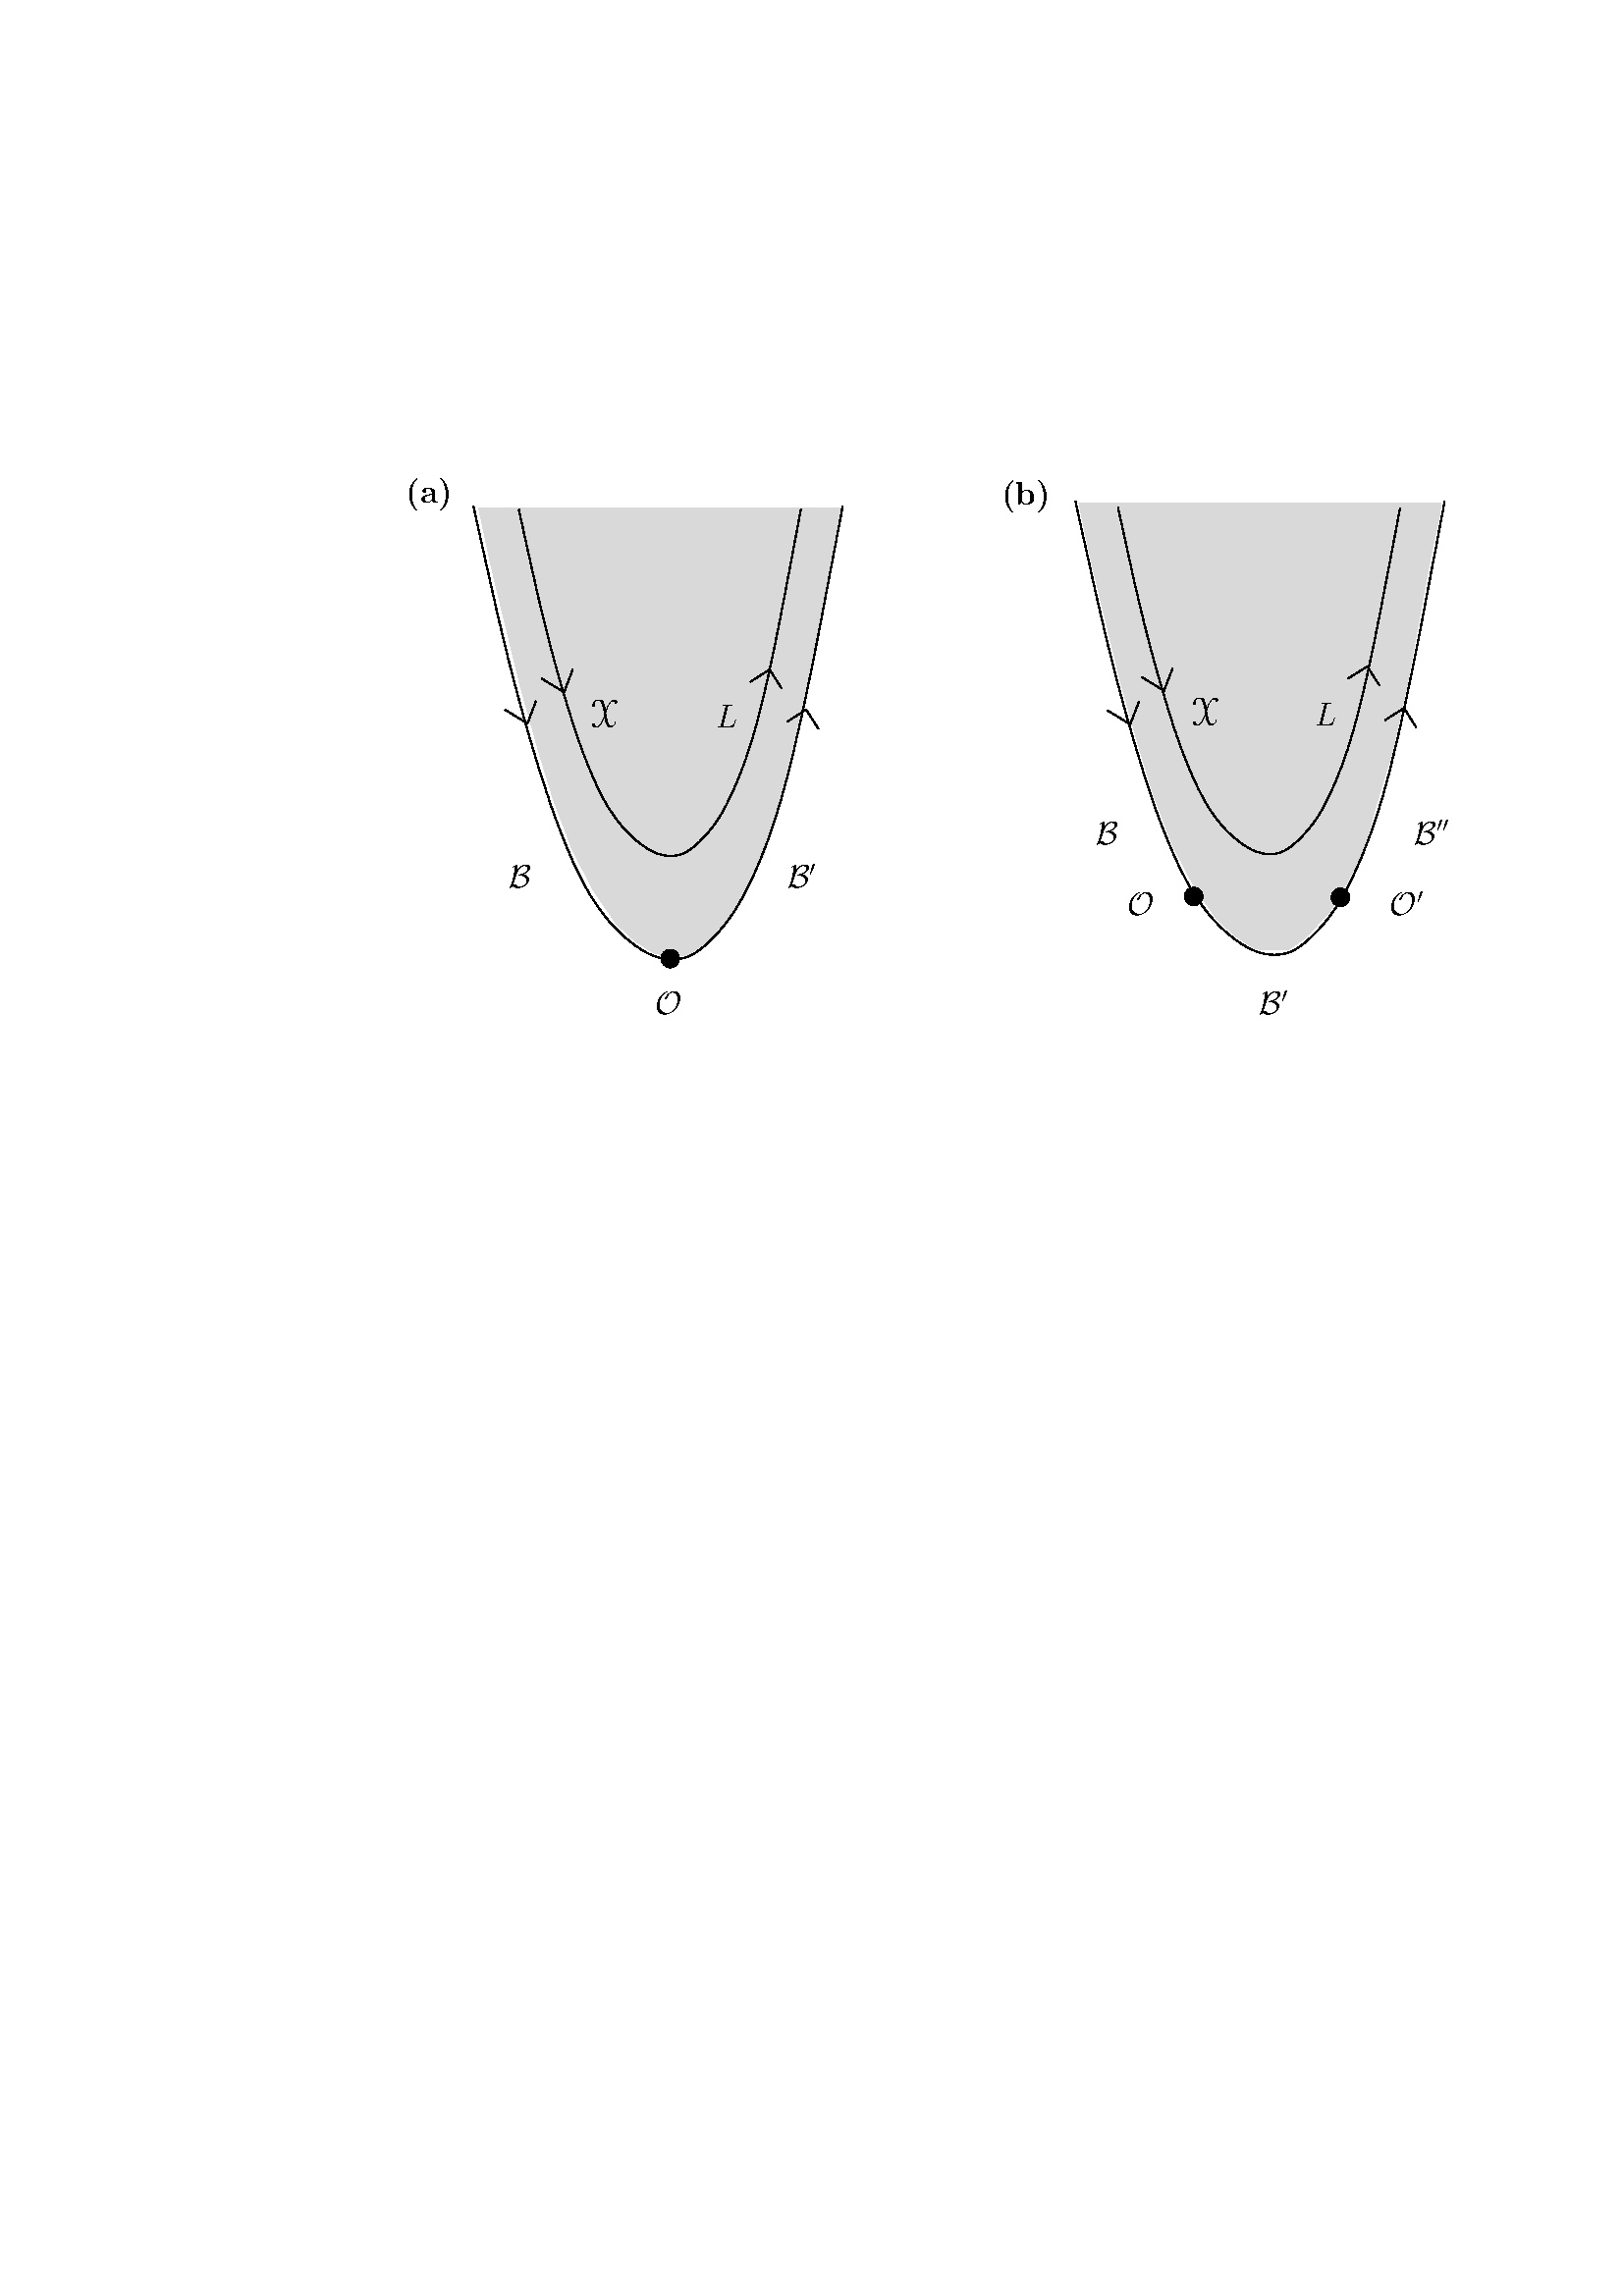
\includegraphics[width=0.75\linewidth]{figures/gla4-6-5.png}
\caption{(a) 支撑在线 $L$ 上的线算子 $\EUX$ 把膜 ${\cal B}$ 与 ${\cal B}'$ 映为膜 $\EUX{\cal B}$ 与 $\EUX{\cal B}'$，同样把 $({\cal B},{\cal B}')$ 弦映为 $(\EUX{\cal B},\EUX{\cal B}')$ 弦。图中算子 ${\EUO}$ 确定一条 $({\cal B},{\cal B}')$ 弦，它被线算子映为一条 $(\EUX{\cal B},\EUX{\cal B}')$ 弦。(b) 这些映射保持开弦乘法的结合律。（原文 Fig.~10）}
\label{fig:zingop}
\end{figure}
 与线算子 $\EUX$ 相联系的是一个自然映射 $\hat\EUX:{\cal H}_{{\cal
B},{\cal B}'}\to{\cal H}_{\EUX{\cal B},\EUX{\cal B}'}$。$\hat \EUX$ 的定义从 \zingop(a) 应当很清楚。在那幅图中，从微观观点看，算子 ${\EUO}$ 确定 ${\cal H}_{{\cal B},{\cal B}'}$ 中的一个态；但从宏观观点看，当 $L$ 趋近边界时，我们看到的是 ${\cal H}_{\EUX{\cal
B},\EUX{\cal B}'}$ 中的一个态。

恰当地说，若 ${\EUO}$ 是恒等算子的倍数，则边界上不存在 ${\EUO}$ 被插入的特殊点，而在线算子 $\EUX$ 趋近边界之前或之后这都是对的。所以 $\hat\EUX$ 把 ${\cal H}_{{\cal B},{\cal B}}$ 中的恒等元（即对应于恒等算子 ${\EUO}=1$ 的开弦态）映为 ${\cal H}_{\EUX{\cal B},\EUX{\cal B}}$ 中的恒等元。它还保持开弦的乘法。事实上，给定三个膜 ${\cal B}$、${\cal B}'$ 与 ${\cal B}''$，结合乘法 ${\cal H}_{{\cal B},{\cal B}'}\otimes{\cal
H}_{{\cal B}',{\cal B}''}\to {\cal H}_{{\cal B},{\cal B}''}$ 是由如 \dunamp(b) 那样粘接开弦定义的，或者等价地由边界上插入算子的算子乘积展开定义，如 \zingop(b) 所示。这显然与把线算子移到边界处的操作交换。概括这些陈述的漂亮说法是：线算子 $\EUX$ 确定了一个把膜范畴映到自身的函子。

把线算子看作膜范畴的对称性，在 \cite{ref99} 中已从不同的观点独立讨论过。它们与对偶变换的关系将在别处讨论 \cite{ref26}。关于用类 Wilson 算子描述二维共形场论中边界微扰的例子，见 \cite{ref100} 的第 5.5 节。

\par\medskip{\it 线算子与增强超对称}

特殊的 Wilson 或 't Hooft 算子可以具有比我们迄今所声称的更多的超对称。

让我们回到超对称 Wilson 算子的定义 \eqref{eq:ymop}。它是 ${\cal
A}_\mu=A_\mu+i\phi_\mu$ 的函数，所以它在任何保持 $A_\mu+i\phi_\mu$ 不变的超对称下不变。按照场在超对称下变换的微观公式 \eqref{eq:hygo}，在由无穷小参数 $\epsilon$ 生成的超对称下，$A_\mu+i\phi_\mu$ 的变分正比于 $(\Gamma_\mu+i\Gamma_{\mu+4})\epsilon$。$\epsilon$ 生成任意 Wilson 线算子的超对称的条件是：该量对 $\mu=0,\dots,3$ 为零，即
% 式 (6.30)
\setcounter{equation}{29}
\begin{equation}\label{eq:pimbo}
\Gamma_{\mu}\Gamma_{\mu+4}\epsilon=i\epsilon,~\mu=0,\dots,3.
\end{equation}

这个条件只留下一个未破缺的超对称，也就是我们迄今所利用的那一个。

然而，假设 $M=\Sigma\times C$ 且度规为乘积度规。此时，扭化保持 \eqref{eq:zonop} 中所刻画的四个超对称。再考虑定义在形如 $\gamma\times
p$ 的一维流形 ${{\cal S}}$ 上的 Wilson 算子，其中 $\gamma$ 是 $\Sigma$ 中的曲线、$p$ 是 $C$ 中的点。对这类算子（我们称之为特殊 Wilson 算子），条件 \eqref{eq:pimbo}\ 归结为
% 式 (6.31)
\setcounter{equation}{30}
\begin{equation}\label{eq:relfo}
\Gamma_{04}\epsilon=\Gamma_{15}\epsilon=i\epsilon.
\end{equation}

这些条件蕴含 \eqref{eq:zonop} 中的第二个条件，而合并起来的条件组留下两个未破缺的超对称。

我们可以很容易地看出额外超对称意味着什么。特殊 Wilson 算子不依赖于 $\varphi$，所以它们在第~\ref{sec:mhhyper}~节引入的 ${\cal U}_1$ 对称下不变；该对称作用在 Higgs 场上为 $\varphi\to\lambda\varphi$，$|\lambda|=1$。这个对称把复结构 $J$ 旋转到复结构 $K$，从而把复结构 $J$ 中的 $B$-模型映为复结构 $K$ 中的 $B$-模型。因此，这两个超对称分别是复结构 $J$ 与 $K$ 中 $B$-模型的拓扑超荷。而复结构 $I_w$ 中任一个 $B$-模型的拓扑超荷都是它们的线性组合。于是可知，特殊 Wilson 算子就是我们或可称为 $(B,B,B)$ 型线算子的东西，也就是说，它保持 $\MH$ 的每个复结构中 $B$-模型的拓扑超对称。

对特殊 't Hooft 算子——即支撑在同类曲线 ${{\cal S}}$ 上的 't Hooft 算子——我们可以用同样的方式推理。特殊 't Hooft 算子同样不依赖于 $\varphi$，因而在群 ${\cal U}_1$ 下不变。这个群把复结构 $K$ 中的 $A$-模型旋转成复结构 $J$ 中的 $A$-模型。一般的 't Hooft 算子保持复结构 $K$ 中的 $A$-型超对称，所以特殊 't Hooft 算子也保持复结构 $J$ 中的 $A$-型超对称。复结构 $I$ 中 $B$-模型的拓扑超荷是复结构 $J$ 与 $K$ 中 $A$-模型的拓扑超荷的线性组合。所以实际上，特殊 't Hooft 算子属于 $(B,A,A)$ 型，也就是说，它们对复结构 $I$、$J$ 与 $K$ 分别保持所指出的那些拓扑超对称。

这与预期完全一致。$S$-变换把 Wilson 算子映为 't Hooft 算子，而从第~\ref{sec:somespec}~节的表 2 可以看出，它把 $(B,B,B)$ 型超对称映为 $(B,A,A)$ 型超对称。

我们还可以进一步特殊化这一情形：取 $\Sigma$ 上的度规为平直度规，并取 ${{\cal S}}$ 为直线。此时，线算子描述静态外电荷或外磁荷。这种形式的 Wilson 或 't Hooft 算子实际上保持四个超对称。例如，对支撑在沿时间方向的直线上的一条 Wilson 算子，未破缺超对称的条件归结为 $\Gamma_{04}\epsilon=i\epsilon$ 与 $\Gamma_{2367}\epsilon=\epsilon$。这个系统在物理上是合理的（如果我们用 Lorentz 号差来解释它）；它由一个实、正定的 Hilbert 空间以及一个正定、Hermite 的 Hamilton 量 $H$ 描述。四个未破缺的超对称就是前面描述的两个拓扑超荷 $Q_i$（$i=1,2$）及其 Hermite 伴随 $Q^\dagger_i$。它们满足物理的超对称代数 $\{Q_i,Q^\dagger_j\}=2\delta_{ij}H$、$\{Q_i,Q_j\}=0=\{Q^\dagger_i,Q^\dagger_j\}$，其中 $i,j=1,2$。

\begin{yizhu}[易错点]
特征膜的定义 \eqref{eq:intico} 是 $\EUX{\cal B}={\cal B}\otimes V$，而不是 $\EUX{\cal B}\cong{\cal B}$。这里是「本征值」位置的是向量空间 $V$，不是数；当 $V=\Bbb{C}^k$ 时 $\EUX{\cal B}$ 才同构于 $k$ 个 ${\cal B}$ 的直和。更一般地 $V$ 会作为向量丛的纤维随参数变化，所以必须保留整个 $V$ 而不能把它压成维数 $k$。它对应的数学概念是 Beilinson–Drinfeld 的 Hecke 特征层。
\end{yizhu}

\begin{yizhu}[易错点]
$V_p$ 只是局部地与 $p$ 无关：拓扑不变性保证移动 $p$（等价于改变 $C$ 上度规，作用量只差 BRST-平凡项 $\{Q,\cdot\}$）给出 $V_p$ 上的平坦联络，从而局部 $V_p$ 不变；但整体上 $V_p$ 可以是 $C$ 上平坦向量丛的纤维，带有非平凡单值。正是这一点把线算子与几何 Langlands 中的平坦丛联系起来——不要把「局部无关」误读成「整体平凡」。
\end{yizhu}

\begin{yizhu}[易错点]
超对称层级要分清：一般的 Wilson 或 't Hooft 线算子只保 1 个超对称（由 \eqref{eq:pimbo} 给出）；乘积度规下、支撑在 $\gamma\times p$ 上的特殊 Wilson 算子保 2 个，属 $(B,B,B)$ 型；同类特殊 't Hooft 算子也保 2 个，但属 $(B,A,A)$ 型；再把度规取为平直、${{\cal S}}$ 取为直线（静态外电荷/外磁荷）则保 4 个，其代数 $\{Q_i,Q^\dagger_j\}=2\delta_{ij}H$、$\{Q_i,Q_j\}=\{Q^\dagger_i,Q^\dagger_j\}=0$。$S$-变换把 $(B,B,B)$ 映为 $(B,A,A)$，与表 2 一致。
\end{yizhu}

\begin{yizhu}[物理图像]
$(B,B,B)$ 与 $(B,A,A)$ 这两个名字来自三个复结构 $I,J,K$：特殊 Wilson 算子不依赖 $\varphi$，在 ${\cal U}_1$（$\varphi\to\lambda\varphi$）下不变，而 ${\cal U}_1$ 把 $J$ 旋转到 $K$，所以它在 $I,J,K$ 三个复结构中都保持 $B$-模型的拓扑超荷；特殊 't Hooft 算子一般保持 $K$ 中 $A$-型超对称，${\cal U}_1$ 把它转到 $J$ 中的 $A$-型，而 $I$ 中 $B$-模型的超荷是 $J,K$ 中 $A$-模型超荷的线性组合，于是得到 $(B,A,A)$。
\end{yizhu}

\begin{yizhu}[物理图像]
Wilson 算子的 OPE 可以经典地算出，原因正是超对称：超对称使 $L\to L'$ 的极限不必经历量子修正，可以直接令 $L=L'$ 并把 $W(R)W(\tilde R)$ 看成表示张量积 $R\otimes\tilde R$ 的和乐，按不可约分解即得 \eqref{eq:tryo}。对偶的 't Hooft OPE \eqref{eq:hffo} 则要微妙得多：在 Coulomb 分支上其系数由磁荷（最高权之和）支配，被 $^L\bar w$ 支配的表示（相伴表示）的系数无法这样直接推出，它们最终来自 Hecke 修改空间的奇异性。
\end{yizhu}

\begin{yizhu}[物理图像]
线算子作为膜范畴的自函子：$\EUX$ 给出映射 $\hat\EUX:{\cal H}_{{\cal B},{\cal B}'}\to{\cal H}_{\EUX{\cal B},\EUX{\cal B}'}$，它把恒等开弦态映为恒等开弦态，并且保持开弦的乘法（即保持结合律），所以它是一个范畴自函子。这就是「对称性 = 范畴的自等价」在二维 TQFT 中的具体体现，也是后文用 Hecke 函子与 Wilson 函子比较的出发点。
\end{yizhu}

%% ============================================================
%% 分片 19：原文第 7 节「Fluxes and $S$-Duality」（原文 glshort.tex 起于第 5685 行）
%% 由 tools/harvmac2tex.py 从 arXiv 源码（hep-th/0604151v3）自动生成。
%% 只译英文散文；公式、编号、\label、\cite 一律不改。
%% ============================================================

\section{通量与 $S$-对偶}

\label{sec:centertop}

\begin{keytakeaways}
  \begin{itemize}[leftmargin=1.4em,itemsep=2pt,topsep=2pt]
    \item \textbf{物理图像}：规范群的中心 $\CZ=\pi_1(G_{\rm ad})$ 是有限阿贝尔群，并且具有自然的自对偶；这使离散磁通量 ${\bf m}$ 与离散电通量 ${\bf e}$ 可以取遍互为对偶的有限群 ${\bf M}$、${\bf E}$，从而让 $S$-对偶在量子理论中得以实现。
    \item \textbf{数学工具}：把理论放在 $M=S^1\times W$ 上，$\Gad$-丛的特征类 $\xi(E)$ 分解为 ${\bf a}\in H^1(W,\CZ)$ 与 ${\bf m}\in H^2(W,\CZ)$ 两部分；庞加莱对偶给出完美配对 $H^1(W,\CZ)\times H^2(W,\CZ)\to U(1)$，故二者互为对偶的有限阿贝尔群。
    \item \textbf{关键结论}：固定 ${\bf m}$ 有 Hilbert 空间解释，固定 ${\bf a}$ 则没有，因此须对 ${\bf a}$ 作傅里叶变换、引入特征标 ${\bf e}$，得到 ${\cal H}_{{\bf e},{\bf m}}$；$S$-对偶交换 ${\bf E}$ 与 ${\bf M}$，把 $({\bf e},{\bf m})$ 送到 $(-{\bf m},{\bf e})$，并把 $\tau$ 送到 $-1/\tau$。
    \item \textbf{边界与展望}：泛丛对伴随群 $G_{\rm ad}$ 存在，对单连通覆盖 $\bar G$ 则被非平凡类 $\zeta=\xi(\EUE_{\rm ad})\in H^2(\M,\CZ)$ 所阻碍；但它总可以作为扭化向量丛存在。
  \end{itemize}
\end{keytakeaways}

本节我们将考察与规范群中心有关的现象，这些现象对于理解 Hitchin 模空间的 $S$-对偶以及几何 Langlands 纲领是相关的。

我们先在第~\ref{sec:reviewthis}~节回顾离散电通量与磁通量以及 $S$-对偶对它们的作用。更多细节可参看 \cite{ref45} 第 3 节以及 \cite{ref26}。关于规范场论中的离散电、磁通量，原始文献是 \cite{ref101}。我们还会解释一些数学概念，例如泛丛的概念。然后在第~\ref{sec:comptwop}~节展开我们的应用。

\subsection{回顾}

\label{sec:reviewthis}

本节中，$G$ 表示紧半单李群；$\bar G$ 是它的万有覆盖；$G_{\rm {ad}}$ 是对应的伴随群。$\bar G$ 的中心（它同时也是 $G_{\rm {ad}}$ 的基本群）是一个有限阿贝尔群 $\CZ$。对于单的 $G$，除 $\bar G=Spin(4n)$ 外，$\CZ$ 在所有情形下都是循环群，如表中所列。

从表中可以注意到一个令人欣慰的事实：对于非单连通型（non-simply-laced）的群，$S$-对偶的某些微妙之处无关紧要，因为 $G_2$ 与 $F_4$ 的中心是平凡的。

\begin{yizhu}[术语]
按：simply-laced（各根等长，A、D、E 型）本文译作「单连通型」，与 simply connected（单连通的）只差一字；两者英文原词不同，阅读时须按上下文区分。本节的「单连通覆盖 $\bar G$」指的是后者。
\end{yizhu}

\par\medskip

\begin{table}[htbp]
\centering
\begin{tabular}{ll}
\toprule
群 & 中心 \\
\midrule
$SU(N)$ & $\Bbb{Z}_N$ \\
$Spin(2n+1)$ & $\Bbb{Z}_2$ \\
$Spin(4n+2)$ & $\Bbb{Z}_4$ \\
$Spin(4n)$ & $\Bbb{Z}_2\times\Bbb{Z}_2$ \\
$Sp(n)$ & $\Bbb{Z}_2$ \\
$E_6$ & $\Bbb{Z}_3$ \\
$E_7$ & $\Bbb{Z}_2$ \\
\bottomrule
\end{tabular}
\caption{具有非平凡中心的单连通单李群。表中略去的 $F_4$、$G_2$ 与 $E_8$ 有平凡中心。（原文 Table~3；原文此处误作 $F_2$、$G_4$）}
\label{tab:centers}
\end{table}

一个重要性质是：群 ${\cal Z}$ 自然地自对偶。阿贝尔群 $B$ 的对偶是 $B^\vee={\rm Hom}(B,U(1))$。有限阿贝尔群总与它自己的对偶同构，但并不是自然地同构。然而 $\bar G$ 的中心 $\CZ$ 总具有自然的自对偶。这一对偶最好用同态 % 式 (7.1)
\setcounter{equation}{0}
\begin{equation}\label{eq:plook}
\Upsilon:\CZ\times \CZ\to
U(1),
\end{equation}
来表达，它是对称的，即 $\Upsilon(a,b)=\Upsilon(b,a)$，并且使得 $\CZ$ 到 $U(1)$ 的任一同态都可写成 $a\to \Upsilon(a,b)$，其中 $b$ 唯一。这样的 $\Upsilon$ 称为「完美配对」。$\Upsilon$ 的构造如下。若 $G$ 是单连通型，则 $\CZ=\Lambda^\vee/\Lambda$，其中 $\Lambda$ 是 $\bar G$ 的根格，$\Lambda^\vee$ 是权格。此时配对 $\Upsilon$ 定义为
% 式 (7.2)
\setcounter{equation}{1}
\begin{equation}\label{eq:rofo}
\Upsilon(a,b)=\exp(2\pi i\langle a,b\rangle),
\end{equation}
其中 $\langle~,~\rangle$ 是 $\Lambda^\vee$ 上通常的二次型（它在 $\Lambda$ 上的限制是偶的、整值的，并在 $\Lambda^\vee$ 上取有理值）。若 $G$ 不是单连通型，则它的中心平凡或为 $\Bbb{Z}_2$，于是恰好容许一种自对偶，我们称之为 $\Upsilon$。

$M$ 上的 $\Gad$-丛 $E$ 有一个特征类 $\xi(E)$，取值于 $H^2(M,\CZ)$。例如若 $G_{{\rm ad}}=SO(3)$，则 $\xi(E)$ 是第二 Stieffel-Whitney 类 $w_2(E)$。对每一种 $\xi$ 的选取，都可以通过把路径积分限制到具有给定 $\xi$ 的丛上来定义配分函数 $Z_\xi$。这些 $Z_\xi$ 按 $S$-对偶群的幺正表示变换 \cite{ref45,ref26}，但这一点我们在此不作解释。

\begin{yizhu}[原文疑误]
按：原文拼作 Stieffel-Whitney，通行拼法为 Stiefel-Whitney（施蒂费尔-惠特尼类）；这里指的是第二 Stiefel-Whitney 类 $w_2(E)$。
\end{yizhu}

我们转而集中于哈密顿描述，并取 $M=S^1\times W$，其中 $W$ 是三维流形。此时有 $H^2(M,\CZ)=H^1(W,\CZ)\oplus H^2(W,\CZ)$，因此 $\xi(E)$ 可以分解为 $\xi={\bf a}\oplus {\bf m}$，其中 ${\bf a}\in H^1(W,\CZ)$，${\bf m}\in H^2(W,\CZ)$。

\begin{yizhu}[物理图像]
按：这里的「通量」是拓扑（离散）数据，而不是场强通量：${\bf m}\in H^2(W,\CZ)$ 是绕 $W$ 中闭曲面的磁通量，${\bf a}\in H^1(W,\CZ)$ 是沿 $S^1$ 方向、与 $W$ 中闭曲线相配对的对应量；二者是同一个特征类 $\xi(E)$ 的两个分量。参见 Witten 2008 综述中关于离散通量与对偶群的讨论。
\end{yizhu}

考虑配对 % 式 (7.3)
\setcounter{equation}{2}
\begin{equation}\label{eq:junko}
\hat \Upsilon:H^2(M,\CZ)\times
H^2(M,\CZ)\to H^4(M,U(1))=U(1)
\end{equation}
它由把上积 $H^2(M,\CZ)\times H^2(M,\CZ)\to H^4(M,\CZ\times\CZ)$ 与映射 $\Upsilon:\CZ\times\CZ\to U(1)$ 复合而得。按庞加莱对偶，$\hat\Upsilon$ 是完美配对，从而使 $H^2(M,\CZ)$ 成为自对偶阿贝尔群。更一般地，对 $n$ 维闭定向流形 $Y$，庞加莱对偶连同 $\CZ$ 的自对偶给出完美配对
% 式 (7.4)
\setcounter{equation}{3}
\begin{equation}\label{eq:unko}
H^d(Y,\CZ)\times H^{n-d}(Y,\CZ)\to U(1), ~~0\leq d\leq
n.
\end{equation}
特别地，我们有完美配对
% 式 (7.5)
\setcounter{equation}{4}
\begin{equation}\label{eq:normo}
\bar\Upsilon:H^1(W,\CZ)\times H^2(W,\CZ)\to U(1).
\end{equation}
所以它们是互为对偶的阿贝尔群，特别地
% 式 (7.6)
\setcounter{equation}{5}
\begin{equation}\label{eq:junok}
H^2(W,\CZ)={\rm Hom}(H^1(W,\CZ),U(1)).
\end{equation}

现在我们来回顾 $S$-对偶如何在哈密顿框架中实现。指定了 ${\bf m}$ 的规范场论配分函数有自然的 Hilbert 空间解释，因为 ${\bf m}$ 是初始时刻数据的一部分，并且与时间无关。然而，由于 ${\bf a}$ 不能由固定时刻的数据表达出来，固定 ${\bf a}$ 的配分函数不能赋予哈密顿解释。于是必须引入有限阿贝尔群 $H^1(M,\CZ)$ 的一个特征标 ${\bf e}$，即同态
% 式 (7.7)
\setcounter{equation}{6}
\begin{equation}\label{eq:kilno}
{\bf e}:H^1(W,\CZ)\to U(1).
\end{equation}
对每一组 ${\bf e}$ 与 ${\bf m}$ 的选取，和 $\sum_{{\bf a}}{\bf e}({\bf a})Z_{{\bf a},{\bf m}}$ 都可以解释为某个 Hilbert 空间 ${\cal H}_{{\bf e},{\bf m}}$ 中的迹。这个和有 Hilbert 空间解释，是因为以权因子 ${\bf e}({\bf a})$ 对 ${\bf a}$ 求和与沿 $S^1$ 方向的切割、粘合（量子场论中通常称为集团分解）相容。${\bf e}$ 与 ${\bf m}$ 分别称为离散电通量与离散磁通量 \cite{ref101}。由 \eqref{eq:junok}，${\bf e}$ 也可以等价地看作 $H^2(W,\CZ)$ 中的一个元素，正如 ${\bf m}$ 一样。

\begin{yizhu}[原文疑误]
按：原文正文说特征标 ${\bf e}$ 是 $H^1(M,\CZ)$ 的同态，而紧随其后的式 (7.7) 写作 $H^1(W,\CZ)\to U(1)$。既然 ${\bf a}\in H^1(W,\CZ)$，对偶的特征标应定义在 $H^1(W,\CZ)$ 上；原文此处疑把 $W$ 写成了 $M$。译文照原文保留了这一措辞。
\end{yizhu}

于是对每一组
% [WARN] 公式 \eqn\eqref{eq:ytro} 无编号或重复
\begin{equation*}
\tag*{(7.8)}
\begin{aligned}{\bf e}&\in {\bf E}={\rm
Hom}(H^1(W,\CZ), U(1))\\
                             {\bf m}& \in {\bf M}=H^2(W,\CZ).
\end{aligned}
\end{equation*}
的选取，我们都得到一个 Hilbert 空间 ${\cal H}_{{\bf m},{\bf e}}$。所幸由 \eqref{eq:junok}，有限群 ${\bf E}$ 与 ${\bf M}$ 同构。这使得 $S$-对偶对称性成为可能。对偶变换 $S$ 交换 ${\bf E}$ 与 ${\bf M}$，并把 $({\bf e},{\bf m})\to (-{\bf m},{\bf e})$：
% 式 (7.9)
\setcounter{equation}{8}
\begin{equation}\label{eq:coco}
S:{\cal H}_{{\bf e},{\bf m}}\to {\cal H}_{-{\bf m},{\bf
e}}.
\end{equation}
当然，它还把 $\tau\to -1/\tau$。（式 \eqref{eq:coco} 是 \eqref{eq:xilj} 的离散类比，其中 $(\vec{\eurm m},\vec{\eurm n})$ 换成了它们的离散对应物 $({\bf m},{\bf e})$。）

\begin{yizhu}[物理图像]
按：$S$ 把固定 $({\bf e},{\bf m})$ 的扇区送到 $(-{\bf m},{\bf e})$，即交换电、磁通量并带一个符号；这与连续理论中 $S:\tau\to-1/\tau$ 以及 $(E,B)\to(B,-E)$ 的变换互为影子。参见 Witten 2008 综述。
\end{yizhu}

虽然可以定义所有这些 Hilbert 空间 ${\cal H}_{{\bf e},{\bf m}}$，但给定的规范场论构造未必用到全部。若我们在 $M=S^1\times W$ 上以单连通规范群 $\bar G$ 作规范场论，则必须把进入配分函数 $Z_{{\bf a},{\bf m}}(M)$ 的特征类 ${\bf a}$ 与 ${\bf m}$ 置零。在 Hilbert 空间层面，这意味着 ${\bf e}$（它由关于 ${\bf a}$ 的傅里叶变换产生）任取，而 ${\bf m}=0$。于是 % 式 (7.10)
\setcounter{equation}{9}
\begin{equation}\label{eq:ytoto}
{\cal H}(\bar G,W)=\oplus_{{\bf e}}{\cal
H}_{{\bf e},0}.
\end{equation}
计及假定下的 ${\bf e},{\bf m}$ 在 $S$-对偶下的变换律，我们看到对偶理论的 Hilbert 空间必为 % 式 (7.11)
\setcounter{equation}{10}
\begin{equation}\label{eq:momjo}
\oplus_{{\bf
m}}{\cal H}_{0,{\bf m}}.
\end{equation}
这个 Hilbert 空间与 $M=S^1\times W$ 上的路径积分有何关系？令 ${\bf e}$ 为零意味着对 ${\bf a}$ 求和。因此在变量 ${\bf a},{\bf m}$ 的表述下，\eqref{eq:momjo} 意味着必须以相同的权重对所有 ${\bf a},{\bf m}$ 求和。换言之，在对偶理论中我们对具有一切可能 $\xi$ 的 $^L\Gad$-丛求和。于是对偶理论的规范群为 $^L\Gad$，正如所期。

\par\medskip\emph{泛丛}

我们还需要另一项背景知识，即泛丛的概念。

先考虑黎曼面 $C$ 上 $G$-丛的模空间 $\M(G,C)$。对每个点 $p\in \M(G,C)$，都有相应的一个由 $p$ 参数化的 $G$-丛 $E_p\to C$；它在同构意义下由 $p$ 确定。泛丛（若存在）是一个 $G$-丛 ${\EUE} \to \M\times C$，使得对任意 $p\in \M$，${\EUE}$ 限制到 $p\times C$ 上都同构于 $E_p$。规范场论给出 \cite{ref91} 一个分析泛丛的非常直接的途径，但我们在此不作解释。

朴素地，我们只需这样定义 ${\EUE}$：使其限制到 $p\times C$ 上就是由 $p$ 决定的 $C$ 上「那个」丛。问题之所以出现，是因为首先 $p$ 只决定 $C$ 上 $G$-丛的同构类，而不是一个具体的丛。这在局部不会造成困难\footnote{这一陈述在 $\M$ 的光滑点附近成立。比本文更精细的分析表明，阻碍泛丛的类 $\zeta(\EUE_{\rm ad})$ 可以在奇点处有局部贡献。}；我们只需在某个特定的 $p$ 处取同构类中正确的一个丛，然后在小邻域内变形它。于是对每个小开集 $U_i\subset \M$，我们都可以选取一个泛丛 ${\EUE}_i\to U_i\times C$，而且 ${\EUE}_i$ 在同构意义下唯一。

下一步是把这些 ${\EUE}_i$ 在 $(U_i\cap U_j)\times C$ 上粘起来。${\EUE}_i$ 与 ${\EUE}_j$ 在 $(U_i\cap U_j)\times C$ 上同构，所以我们在这个交叠上选取同构 $\Theta_{ij}:{\EUE}_i\cong {\EUE}_j$，并令 $\Theta_{ji}=\Theta_{ij}^{-1}$。

现在，如果在三重交叠 $(U_i\cap U_j\cap U_k)\times C$ 上复合 $\Theta_{ki}\Theta_{jk}\Theta_{ij}$ 等于 1，那么我们就可以相容地把这些 ${\EUE}_i$ 粘起来，得到所要的泛丛 ${\EUE}$。

若规范群是伴随群 $G_{{\rm ad}}$，粘合没有问题。一般的 $G_{{\rm ad}}$-丛没有自同构（例外出现在 $\M$ 的奇点处）。因此 $\Theta_{ki}\Theta_{jk}\Theta_{ij}$ 由于是 ${\EUE}_i$（限制到 $(U_i\cap U_j\cap U_k)\times C$）到自身的同构，在三重交叠的一般点上等于恒等，从而处处等于恒等。

于是，泛 $G_{{\rm ad}}$-丛 ${\EUE}_{\rm {ad}}$ 确实存在。现在我们把规范群换成单连通覆盖 $\bar G$（更一般地，换成 $G_{\rm{ad}}$ 的任意具有非平凡中心的覆盖）来重复这一讨论。我们从同样的方式开始。对每个小开集 $U_i\in \M$，选取 $U_i\times C$ 上的泛丛 $\bar {\EUE}_i$，并试图把它们粘成泛 $\bar G$-丛 $\bar {\EUE}$。

结果之所以不同，是因为一般的 $\bar G$-丛确实有非平凡的自同构群；中心 $\CZ$ 是任意 $\bar G$-丛 $E$ 的一个自同构群。

因此在上面的论证中，三重交叠上的复合映射 $\Theta_{ki}\Theta_{jk}\Theta_{ij}$ 未必是恒等；而是 % 式 (7.12)
\setcounter{equation}{11}
\begin{equation}\label{eq:yrf}
\Theta_{ki}\Theta_{jk}\Theta_{ij}=f_{ijk},
\end{equation}
其中 $f_{ijk}\in\CZ$。这些 $f_{ijk}$ 组成一个二维闭链，定义了一个元素 $\zeta\in H^2(\M,\CZ)$。已知 $\zeta$ 是非平凡的；它是泛 $\bar G$-丛 $\bar{\EUE}$ 存在性的障碍。

\begin{yizhu}[易错点]
按：障碍 $\zeta$ 是 $H^2(\M,\CZ)$ 中的类，而不是 $H^1$ 中的类；它来自三重交叠上 $\Theta_{ki}\Theta_{jk}\Theta_{ij}\in\CZ$ 的粘合失败。$G_{\rm ad}$-丛没有自同构，故无此问题；$\bar G$-丛的全纯中心 $\CZ$ 自同构正是根源。
\end{yizhu}

还有另一种方式解释 $\zeta$ 的存在。设 $\M(G_{\rm{ad}},C)_0$ 是 $\M(G_{\rm{ad}},C)$ 中参数化拓扑平凡丛的分支——这些丛限制到 $p\times C$（$p\in \M(G_{\rm{ad}},C)$）上时可以提升为 $\bar G$-丛。考虑 $\M(G_{\rm{ad}},C)_0\times C$ 上的泛丛 ${\EUE}_{\rm{ad}}$。如果我们能把 ${\EUE}$ 提升为 $\bar G$-丛 $\bar {\EUE}$，那么（把它拉回到 $\M(\bar G,C)\times C$，后者是 $\M(G_{\rm {ad}},C)_0\times C$ 的有限覆盖）这就是泛 $\bar G$-丛。一般地，把 $G_{\rm ad}$-丛 ${\EUE}_{\rm{ad}}$ 提升为 $\bar G$-丛 $\bar {\EUE}$ 的障碍是特征类 $\xi({\EUE}_{\rm{ad}})$。所以泛 $\bar G$-丛存在性的障碍是 $\zeta=\xi({\EUE}_{\rm {ad}})$。

对 Higgs 丛有类似的故事。泛 Higgs 丛是一个对 $( {\EUE},\hat \varphi)$，其中 $ {\EUE} $ 是 $\MH(G,C)\times C$ 上的 $G$-丛，$\hat\varphi\in H^0( \MH(G,C)\times C,{\rm {ad}}({\EUE})\otimes K_C)$，并满足如下条件：对每个 $p\in \MH(G,C)$，$( {\EUE},\hat\varphi)$ 限制到 $p\times C$ 上应当同构于由 $p$ 参数化的 Hitchin 对 $(E_p,\varphi_p)$。

把已经给出的论证原封不动地搬过来，即可证明对规范群 $G_{\rm{ad}}$，泛 Higgs 丛 $( {\EUE}_{\rm {ad}},\hat\varphi)$ 确实存在。但对单连通规范群 $\bar G$（或 $G_{\rm {ad}}$ 的任一非平凡覆盖），泛 Higgs 丛不存在。其障碍在于：一般的 Hitchin 对 $(E,\varphi)$（其中 $E$ 为 $\bar G$-丛）具有自同构群 $\CZ$。这个障碍正是把泛 $G_{{\rm ad}}$ Higgs 丛 $({\EUE}_{\rm{ad}},\hat\varphi)$ 的「丛」部分提升为 $\bar G$-丛的障碍。因此它是
% 式 (7.13)
\setcounter{equation}{12}
\begin{equation}\label{eq:plooo}
\zeta=\xi({\EUE}_{\rm{ad}}).
\end{equation}

\par\medskip\emph{泛丛作为扭化向量丛}

虽然对非伴随型的 $G$，泛 $G$-丛作为向量丛或主丛不存在，但它作为扭化向量丛确实存在。我们将以一种非常初等的方式来描述这个概念。

构造流形 $X$ 上秩为 $N$ 的普通向量丛 $V$ 的一种办法是：用小的开集 $U_i$ 覆盖 $X$，在每个开集上选取秩 $N$ 的平凡丛 $V_i\cong U_i\times \Bbb{C}^N$。然后在交叠 $U_i\cap U_j$ 上用粘合映射 $v_{ij}:V_i\cap V_j\to U(N)$ 把 $V_i$ 粘到 $V_j$，并令 $v_{ji}=v_{ij}^{-1}$。如果在三重交叠上有 % 式 (7.14)
\setcounter{equation}{13}
\begin{equation}\label{eq:nofto}
v_{ki}v_{jk}v_{ij}=1,
\end{equation}
那么这些 $V_i$ 就可以相容地粘成一个秩 $N$ 的向量丛 $V\to X$。

现在假设给定 $b\in H^2(X,U(1))$。则 $b$ 可以由三重交叠 $U_i\cap U_j\cap U_k$ 上定义的 $U(1)$-值闭链 $b_{ijk}$ 显式表示。扭化向量丛由同样类型的数据 $v_{ij}:V_i\cap V_j\to U(N)$ 定义。但现在我们要求的不再是 \eqref{eq:nofto}，而是
% 式 (7.15)
\setcounter{equation}{14}
\begin{equation}\label{eq:hofto}
v_{ki}v_{jk}v_{ij}=b_{ijk}.
\end{equation}
于是，$b$-扭化向量丛 $V$ 不是通常意义上的向量丛。然而，伴随向量丛 ${\rm ad}(V)$ 是普通向量丛，因为一旦转到伴随表示，\eqref{eq:hofto} 中的相位 $b_{ijk}$ 就消失了。

现在回到构造泛丛的问题。本文一般对下面一点稍欠精确：所谓 $G$-丛，究竟是指纤维为 $G$ 的副本的主 $G$-丛，还是在 $G$ 的某个忠实表示下的相伴向量丛。主丛使得对任意 $G$ 都适用的统一分析成为可能；但对像 $U(N)$ 这样具有方便的忠实表示（$N$ 维表示）的群，用向量丛来思考是有益的。

在讨论泛丛时，更精确一些是有帮助的。我们把上面讨论中的过渡函数 $\Theta_{ij}$ 解释为 $\bar G$-值函数，不选取任何特定的表示。它们到 $G_{ad}$ 的投影给出泛主 $G_{ad}$-丛 ${\EUE}_{\rm ad}$ 的过渡函数，但由于关系
% 式 (7.16)
\setcounter{equation}{15}
\begin{equation}\label{eq:flutter}
\Theta_{ki}\Theta_{jk}\Theta_{ij}=f_{ijk},
\end{equation}
其中 $f_{ijk}$ 定义了类 $\zeta=\xi({\EUE}_{ad})\in H^2(\MH(G_{\rm ad},C),\CZ)$，我们无法把它提升为主 $\bar G$-丛。现在取 $\bar G$ 的一个不可约表示 $\varrho$。我们把 $\Theta_{ij}$ 在表示 $\varrho$ 下求值所得的过渡函数记作 $\Theta_{ij}^\varrho$。同样把 $f$ 在表示 $\varrho$ 下求值记作 $\varrho(f)$。在不可约表示 $\varrho$ 中，$\bar G$ 的中心按纯量乘法作用，因此 $\varrho(f)$ 取值于 $U(1)$。我们有
% 式 (7.17)
\setcounter{equation}{16}
\begin{equation}\label{eq:glutter}
\Theta^\varrho_{ki}\Theta^\varrho_{jk}\Theta^\varrho_{ij}=\varrho(f_{ijk}).
\end{equation}

这些量 $\varrho(f_{ijk})$ 是一个闭链，定义了元素 $\varrho(\zeta)\in H^2(\MH(G_{\rm ad},C),U(1))$。

若 $\varrho(f)=1$，则这些对象 $\Theta^\varrho$ 就是过渡函数，它们定义了一个向量丛 ${\EUE}_\varrho\to \MH(\bar G,C)\times C$，我们可以称之为表示 $\varrho$ 中的泛丛。一般情形下并非如此。然而，比较式 \eqref{eq:flutter} 与 \eqref{eq:hofto} 可以看出，虽然 ${\EUE}_\varrho$ 可能不作为普通向量丛存在，但它总是作为扭化向量丛存在，其扭化为 $\varrho(\zeta)\in H^2(\MH(G_{\rm ad},C),U(1))$。

\begin{yizhu}[易错点]
按：扭化向量丛的粘合只在三重交叠上差一个 $U(1)$ 相位 $b_{ijk}$，因此它不是通常意义上的丛；但取伴随丛时这个相位消失，故 ${\rm ad}(V)$ 仍是普通向量丛。对泛丛而言，取不可约表示 $\varrho$ 后相位变为 $\varrho(f_{ijk})$，于是 ${\EUE}_\varrho$ 是以 $\varrho(\zeta)$ 扭化的向量丛，而不是普通丛。
\end{yizhu}

%% ============================================================
%% 分片 20：原文第 7 节「Fluxes and $S$-Duality」（原文 glshort.tex 起于第 5685 行）
%% 由 tools/harvmac2tex.py 从 arXiv 源码（hep-th/0604151v3）自动生成。
%% 只译英文散文；公式、编号、\label、\cite 一律不改。
%% ============================================================

\subsection{紧化到二维} \label{sec:comptwop}

现在我们把理论紧化到二维。考虑 $M=\Sigma\times C$ 上规范群为 $G_{\rm{ad}}$ 的 ${\EUN}=4$ 超 Yang-Mills 理论。该理论的数据是 $G_{\rm{ad}}$-丛 $E\to\Sigma\times C$、$E$ 上的联络 $A$ 以及各种其他场。任取 $E$ 都决定一个类 $\xi(E)\in H^2(\Sigma\times C,\CZ)$。由于 $H^2(\Sigma\times C,\CZ)=H^2(\Sigma,\CZ)\oplus H^1(\Sigma,H^1(C,\CZ))\oplus H^2(C,\CZ)$，我们有 % [WARN] 公式 \eqn\eqref{eq:ytro} 无编号或重复
\begin{equation*}
\tag*{(7.18)}
\xi(E)\in H^2(\Sigma,\CZ)\oplus
H^1(\Sigma,H^1(C,\CZ))\oplus
H^2(C,\CZ).
\end{equation*}
相对于这一分解，我们写 $\xi(E)=\xi(E)^{2,0}+\xi(E)^{1,1}+\xi(E)^{0,2}$。

我们可以用低能有效 sigma 模型描述同一件事。这里我们考虑 $\Sigma\times C$ 上的低能数据，当它们限制到 $p\times C$（$p\in \Sigma$）上时，决定 $\MHAD$ 中的一个点。随着 $p$ 变化，我们得到映射 $\Phi:\Sigma\to \MHAD$。把 $\Phi$ 与 $C$ 上的恒等映射复合，得到映射 $\Phi\times 1:\Sigma\times C\to \MHAD\times C$。现在回忆泛丛 ${\EUE}_{\rm ad}$ 与类 $\zeta=\xi({\EUE}_{\rm {ad}})\in H^2( \MHAD\times C,\CZ)$。把它拉回到 $\Sigma\times C$，我们得到类 $(\Phi\times 1)^*(\zeta)\in H^2(\Sigma\times C,\CZ)$。梳理一遍定义即可看出 % 式 (7.19)
\setcounter{equation}{18}
\begin{equation}\label{eq:yrog}
\xi(E)=(\Phi\times
1)^*(\zeta).
\end{equation}
事实上，泛丛 ${\EUE}_{ad}$ 正是这样定义的，使得 $(\Phi\times 1)^*({\EUE}_{{\rm ad}})=E$，所以 $(\Phi\times 1)^*(\zeta)=(\Phi\times 1)^*(\xi(\EUE_{{\rm ad}}))=\xi((\Phi\times 1)^*(\EUE_{{\rm ad}}))=\xi(E)$。

\begin{yizhu}[物理图像]
按：式 (7.18) 按 Künneth 分解把 $\xi(E)$ 分成 $\Sigma$ 与 $C$ 两个方向上的分量，$\xi(E)^{p,q}$ 即 $\Sigma$ 方向 $p$ 次、$C$ 方向 $q$ 次的部分。其中 $\xi(E)^{0,2}={\bf m}_0$ 度量 $E$ 限制到 $C$ 上的拓扑类型，$\xi(E)^{2,0}={\bf a}_0$ 是沿 $\tilde S^1$ 方向的数据；式 (7.19) 说明它们全部是从泛丛的障碍类 $\zeta$ 拉回得到的，这是后文把 $\zeta$ 解释为平坦 $B$-场的基础。
\end{yizhu}

我们进一步取 $\Sigma=S^1\times \tilde S^1$，其中两个因子都是圆周。我们写 $W=\tilde S^1\times C$，于是 $\Sigma\times C=S^1\times W$。$\xi(E)$ 有熟悉的展开 $\xi(E)={\bf a}+{\bf m}$，其中 ${\bf a}\in H^1(W,\CZ)$，${\bf m}\in H^2(W,\CZ)$。但现在我们还可以进一步展开 $H^1(W,\CZ)=H^1(\tilde S^1,\CZ)\oplus H^1(C,\CZ)$，于是有 ${\bf a}={\bf a}_0+{\bf a}_1$，其中 % 式 (7.20)
\setcounter{equation}{19}
\begin{equation}\label{eq:mimot}
\begin{aligned}{\bf
a}_0&\in H^1(\tilde S^1,\CZ) =\CZ,\\ {\bf a}_1& \in
H^1(C,\CZ).
\end{aligned}
\end{equation}
类似地，我们可以展开 $H^2(W,\CZ)=H^1(\tilde S^1,H^1(C,\CZ))\oplus H^2(C,\CZ)$，于是有 ${\bf m}={\bf m}_0+{\bf m}_1$，其中 % 式 (7.21)
\setcounter{equation}{20}
\begin{equation}\label{eq:nimot}
\begin{aligned}{\bf
m}_0&\in H^2(C,\CZ)=\CZ \\
                     {\bf m}_1&\in
                     H^1(\tilde S^1,H^1(C,\CZ))=H^1(C,\CZ).
\end{aligned}
\end{equation}

与展开 \eqref{eq:ytro} 相对照，我们看到
% 式 (7.22)
\setcounter{equation}{21}
\begin{equation}\label{eq:zimot}
\xi(E)^{2,0}={\bf a}_0,~\xi(E)^{0,2}={\bf m}_0.
\end{equation}

我们可以类似地分解与 $\bf a$ 对偶的特征标 $\bf e$。显然有 ${\bf e}={\bf e}_0+{\bf e}_1$，其中 ${\bf e}_0$ 是 ${\bf a}_0\in \CZ$ 的特征标，${\bf e}_1$ 是 ${\bf a}_1\in H^1(C,\CZ)$ 的特征标。因此，利用 $\CZ$ 的自对偶与庞加莱对偶， % 式 (7.23)
\setcounter{equation}{22}
\begin{equation}\label{eq:tew}
\begin{aligned} {\bf e}_0 & \in
\CZ^\vee=\CZ\\ {\bf e}_1&\in H^1(C,\CZ)^\vee=H^1(C,\CZ).
\end{aligned}
\end{equation}
鉴于 \eqref{eq:coco}，$S$-对偶下的变换为
% 式 (7.24)
\setcounter{equation}{23}
\begin{equation}\label{eq:niko}
\begin{aligned}({\bf e}_0,{\bf m}_0)&\to (-{\bf m}_0,{\bf
e}_0)\\ ({\bf e}_1,{\bf m}_1)&\to (-{\bf m}_1,{\bf e}_1).
\end{aligned}
\end{equation}

我们的下一个目标是在靶为 $\MHAD$ 的有效二维 sigma 模型中解释 ${\bf e}_0$、${\bf e}_1$、${\bf m}_0$ 与 ${\bf m}_1$。我们将同时考虑闭黎曼面 $\Sigma$ 的情形与 $\Sigma$ 带边界的情形。后一情形将使我们能够理解 \eqref{eq:niko} 对几何 Langlands 纲领的含义。

\par\medskip\emph{${\bf m}_0$ 的解释}

最容易解释的是 ${\bf m}_0=\xi(E)^{0,2}$。我们 sigma 模型的靶空间 $\MH(G_{\rm ad},C)$ 不连通。它的各连通分支由 $G_{\rm ad}$-丛 $E\to C$ 的拓扑类型标记。而这正是 ${\bf m}_0$ 所度量的。

\par\medskip\emph{${\bf e}_0$ 的解释}

一般地，考虑映到某个流形 $X$ 的映射 $\Phi:\Sigma\to X$ 的 sigma 模型。平坦 $B$-场是元素 $b\in H^2(X,U(1))$。在 $\Sigma$ 无边界的情形，平坦 $B$-场以下述方式进入 sigma 模型路径积分。给定映射 $\Phi:\Sigma\to X$，把 $b$ 拉回为 $\Phi^*(b)\in H^2(\Sigma,U(1))=U(1)$，然后在路径积分中乘入因子 $\Phi^*(b)$。于是，在这种情形下，引入平坦 $B$-场的作用是给 $\Sigma$ 到 $X$ 的不同映射分支赋以相位权重。

现在 ${\bf e}_0$ 在映射 $\Phi:\Sigma\to \MH(G_{\rm ad},C)$ 的 sigma 模型中决定一个平坦 $B$-场。事实上，如我们已经解释过的，存在自然的类 $\zeta\in H^2(\MH(G_{\rm ad},C),\CZ)$，它表示把泛 $G_{\rm{ad}}$-丛 ${\EUE}_{\rm {ad}}\to\MH(G_{\rm ad},C)\times C$ 提升为 $\bar G$-丛的障碍。把 $\zeta$ 与 ${\bf e}_0:\CZ\to U(1)$ 复合，我们得到平坦 $B$-场 $b_{{\bf e}_0}={\bf e}_0(\zeta)\in H^2(\MH(G_{\rm{ad}},C),U(1))$。我们断言：${\bf e}_0$ 在映射 $\Sigma\to \MHAD$ 的有效 sigma 模型中的作用，正是按带平坦 $B$-场 $b_{{\bf e}_0}$ 的 sigma 模型所预期的方式给每个映射赋权。

事实上，${\bf e}_0$ 的定义就是路径积分包含相位因子 ${\bf e}_0({\bf a}_0)={\bf e}_0(\xi(E)^{2,0})$。但 $\xi(E)^{2,0}=\Phi^*(\zeta)$；这可由把 \eqref{eq:yrog} 限制到 $C$ 中一点看出。所以 ${\bf e}_0$ 在路径积分中诱导的相位因子是 ${\bf e}_0(\Phi^*(\zeta))=\Phi^*({\bf e}_0(\zeta))=\Phi^*(b_{{\bf e}_0})$。这就证实了我们的断言：${\bf e}_0$ 在 sigma 模型中的作用是生成平坦 $B$-场 $b_{{\bf e}_0}$。

因此 \eqref{eq:niko} 意味着 $S$-对偶把平坦 $G_{\rm{ad}}$-丛的拓扑类 ${\bf m}_0$ 与由 ${\bf e}_0$ 决定的平坦 $B$-场互换。

\begin{yizhu}[物理图像]
按：这里把两个量分得很清楚：${\bf m}_0$ 是离散拓扑数据，它标记 $\MHAD$ 的连通分支（即 $E$ 在 $C$ 上的拓扑类型）；${\bf e}_0$ 是相位数据，它经由 $\zeta$ 给出平坦 $B$-场 $b_{{\bf e}_0}$，从而给不同映射分支加权。式 (7.24) 说的正是 $S$-对偶把这两者互换。参见 Witten 2008 综述关于离散 $\theta$ 角与 $B$-场的讨论。
\end{yizhu}

\par\medskip\emph{膜的引入}

对于几何 Langlands 纲领的应用而言，真正的收获在于理解这一切对膜的含义。

于是我们取 $\Sigma$ 为带边界的黎曼面。$M=\Sigma\times C$ 因此是带边界 $\partial M=\partial\Sigma\times C$ 的四维流形。在 $\partial M$ 上，我们放置某个超对称边界条件。

有效的二维描述是映射 $\Phi:\Sigma\to \MHAD$ 的 sigma 模型，其边界条件对应某个膜。我们想理解 ${\bf e}_0$ 与 ${\bf m}_0$ 在这一描述中的作用。

关于 ${\bf m}_0$ 没有什么新东西可说。无论 $\Sigma$ 是否有边界，它都标记 $\MHAD$ 的连通分支。

${\bf e}_0$ 的作用则更微妙。如我们所见，靶为 $\MHAD$ 的 sigma 模型配备有平坦 $B$-场 ${\bf e}_0(\zeta)$。平坦 $B$-场对膜有非常有趣的影响 \cite{ref102}。没有 $B$-场时，$\MHAD$ 上的膜有 Chan-Paton 丛，它是 $\MHAD$ 上的向量丛（更一般地，是可能支撑在子流形上的层，它定义 $\MHAD$ 的一个 $K$-理论类）。然而，当存在平坦 $B$-场（对应元素 $b\in H^2(\MHAD,U(1))$）时，Chan-Paton 丛变成扭化向量丛（更一般地，是与 $\MHAD$ 的扭化 $K$-理论中某元素相关的扭化层），其扭化由 $b$ 按式 \eqref{eq:hofto} 的意义给出。正是因为这个，我们才引入了扭化向量丛的概念。

所以简而言之，当 ${\bf e}_0\not=0$ 时，膜的 Chan-Paton 丛是扭化向量丛，扭化为 $b_{{\bf e}_0}={\bf e}_0(\zeta)$。所幸，由第~\ref{sec:reviewthis}~节末的分析，我们有大量这样的扭化向量丛可用。若 $\varrho$ 是 $\bar G$ 的任意不可约表示，使得由 $\varrho$ 定义的 $\bar G$ 中心的特征标等于 ${\bf e}_0$，则表示 $\varrho$ 中的泛丛 ${\EUE}_\varrho$ 就是平坦 $B$-场 $b_{{\bf e}_0}$ 的一个扭化向量丛的例子。

其他重要的扭化膜例子可以这样构造：选取子流形 $Y\subset \MHAD$，使得 $b_{{\bf e}_0}$ 限制到 $Y$ 上平凡。此时，支撑在 $Y$ 上的膜的定义与 ${\bf e}_0$ 无关（相差一个并不完全典范的同构）。例如，$Y$ 可以是 $\MHAD$ 中的一点。$b_{{\bf e}_0}$ 限制到一点上当然是平凡的，所以对任意 ${\bf e}_0$，零膜都存在。由这样的零膜，我们可以构成电特征膜，这将在第~\ref{sec:electricbranes}~节解释。稍微更微妙的例子是磁特征膜，即支撑在 Hitchin 纤维化的一条纤维 ${\CMF}$ 上的秩一膜。这种膜的 Chan-Paton 丛应当是平坦\footnote{这里可以把「平坦」理解为与普通线丛一样，即过渡函数是常数。}扭化线丛。文献 \cite{ref21} 证明了平坦 $b$-场 $b_{{\bf e}_0}$ 限制到 ${\CMF}$ 上平凡，因此平坦扭化线丛的空间与 ${\CMF}$ 上普通平坦线丛的空间同构，但并非典范同构。

现在我们可以从 $S$-对偶推出一个关于膜的陈述。对偶变换 $S$ 把 $({\bf e}_0,{\bf m}_0)\to (-{\bf m}_0,{\bf e}_0)$，所以它把「膜所支撑的 $\MH$ 分支的拓扑」与「其 Chan-Paton 丛扭化所依据的平坦 $B$-场 $b_{{\bf e}_0}$」互换。当然，它还把 $G_{\rm ad}$ 与\footnote{所谓 $^L\negthinspace G_{\rm ad}$，我们指群 $^L\negthinspace G$ 的伴随形式。这里描述的陈述最好用双侧的伴随丛来表述，以便容许所有可能的拓扑。我们只在暂时需要时会明确说明，所取的是 $\MH$ 的某个分支还是它的万有覆盖。} $^L\negthinspace G_{{\rm ad}}$ 互换，并且（如我们在本节结尾评注中所解释的）把 $\MH(G_{{\rm ad}})$ 与 $\hat\M_H({}^L\negthinspace G_{{\rm ad}})$ 互换，后者我们定义为 $\MH({}^L\negthinspace G_{{\rm ad}})$ 的万有覆盖。

作为这种对偶的特例，一侧位于 Hitchin 纤维化某条纤维 ${\CMF}$ 中的一点，被映射到另一侧支撑在 Hitchin 纤维化相应纤维 $^L\negthinspace{\CMF}=\Xi({\CMF})$ 上、并配有平坦扭化线丛的秩一膜。${\CMF}$ 是一族复环面之并，由 Higgs 丛的特征类 ${\bf m}_0=\xi(E)$ 标记。一侧 ${\CMF}$ 分支的选取，决定了另一侧的离散电场 ${\bf e}_0$，从而决定了扭化。${\CMF}$ 上一点的选取，决定了 $^L\negthinspace{\CMF}$ 上的平坦扭化线丛（在 $S$-对偶变换下它被映到那里）。当然，${\CMF}$ 与 $^L\negthinspace{\CMF}$ 之间的这种关系是相互的。${\CMF}$ 与 $^L\negthinspace{\CMF}$ 之间的这种扭化对偶，实际上是 Hausel 与 Thaddeus \cite{ref21} 的主要结果之一。

\begin{yizhu}[易错点]
按：$^L\negthinspace G_{\rm ad}$ 指 Langlands 对偶群 $^L\negthinspace G$ 的伴随形式，而不是 $G_{\rm ad}$ 本身的 Langlands 对偶群。原文选择在两侧都用伴随丛来陈述对偶，是为了容纳所有可能的拓扑；否则就得同时选定 $\MH$ 的某个分支或它的万有覆盖。$\hat\M_H$ 是 $\MH$ 的万有覆盖，两者的区别在第 7.2 节末的评注中还会出现。
\end{yizhu}

\par\medskip\emph{${\bf e}_1$ 与 ${\bf m}_1$ 的解释}

最后让我们用二维的语言讨论 ${\bf e}_1$ 与 ${\bf m}_1$ 的解释。先比较规范群为 $\bar G$ 与 $G_{\rm{ad}}$ 的两个理论会有帮助。

$\MH(\bar G)$ 是单连通的。它有一个自然的对称群 ${\bf E}_C=H^1(C,\CZ)$。事实上，${\bf E}_C$ 参数化 $C$ 上的 $\CZ$-丛。一个 $\bar G$ Higgs 丛 $(E,\varphi)$ 可以与一个 $\CZ$-丛作张量积，得到新的 $\bar G$ Higgs 丛。（具体地说，这个操作把 $E$ 绕 $C$ 中非可缩闭圈的 holonomy 乘以 $\bar G$ 中心的元素。）所以这给出靶为 $\MH(\bar G)$ 的 sigma 模型的一个对称群 ${\bf E}_C$。该 sigma 模型的 Hilbert 空间可以按 ${\bf E}_C$ 的特征标分解。

另一方面，$\MHAD$ 没有这样的几何对称性。但它有基本群 ${\bf M}_C=H^1(C,\CZ)$，与 ${\bf E}_C$ 同构。要理解这个基本群从何而来，一个捷径是注意到 $\MHAD$ 的一个分支 $\MHAD_0$，即参数化可提升为 $\bar G$ 的 Higgs 丛的那个分支，恰好是 $\MHAD_0=\MH(\bar G)/{\bf E}_C$。除以 ${\bf E}_C$ 消去了 $\MH(\bar G)$ 的几何对称性，但当然也产生了基本群。\footnote{${\bf E}_C$ 的作用并不自由，所以 $\M_H(G_{ad})$ 有轨形奇点。（它还有来自可约 Higgs 丛的更严重奇点。）正如 sigma 模型中所熟悉的，$\M_H(G_{ad})$ 的基本群必须在轨形意义下理解。或者，也可以依赖四维规范场论，而不必约化到带有奇点的 sigma 模型。}所以 $\pi_1(\MHAD_0)\cong {\bf E}_C$。

实际上，$\MHAD$ 任一连通分支的基本群都相同。$\MHAD$ 的定义是：把规范群为 $G_{\rm {ad}}$ 的 Hitchin 方程的所有解空间，除以 $C$ 上所有 $G_{\rm{ad}}$-值规范变换构成的群 ${\cal G}_{\rm{ad}}(C)$。如果只除以 ${\cal G}_{\rm{ad}}(C)$ 的连通分支，得到的就是万有覆盖 $\hat\M_H(G_{\rm {ad}},C)$。因此 $\MHAD$ 的基本群就是 ${\cal G}_{\rm ad}(C)$ 的分支群，而对 $\MHAD$ 的任一分支，这个群都是 ${\bf E}_C=H^1(C,\CZ)$。

总之，在 $\MHAD$ 上运动的弦有一个离散的守恒缠绕数群 ${\bf M}_C=\pi_1(\MHAD)=H^1(C,\CZ)$。同样，在 $\MH(\bar G)$ 上运动的弦有一个离散的守恒动量群 ${\bf E}_C=H^1(C,\CZ)$。

让我们把对称性 ${\bf E}_C$ 与 ${\bf M}_C$ 同我们在底层规范场论中能看到的东西作比较。在 $M=\Sigma\times C=S^1\times \tilde S^1\times C$ 上的 $G_{\rm{ad}}$ 规范场论中，丛 $E$ 及其他数据决定映射 $\Phi:S^1\times \tilde S^1\to \MHAD$。在分析这一情形的拓扑时，我们把特征类 $\xi(E)$ 展开为 $\xi(E)={\bf a}\oplus {\bf m}$，其中 ${\bf m}$ 是 $\xi(E)$ 在 $\tilde S^1\times C$ 上的限制（更确切地说，是针对 $p\in S^1$ 限制到 $p\times \tilde S^1\times C$）。在低能 sigma 模型中，${\bf a}$ 与 ${\bf m}$ 是 $\Phi:\Sigma\to \MHAD$ 的不变量。特别地，${\bf m}$ 只依赖于 $\Phi$ 在 $\tilde S^1$ 上的限制 $\Phi|_{\tilde S^1}$。

在 \eqref{eq:nimot} 中，我们进一步展开了 ${\bf m}={\bf m}_0\oplus {\bf m}_1$，其中 ${\bf m}_1\in H^1(\tilde S^1,H^1(C,\CZ))$。${\bf m}_1$ 是 $\Phi|_{\tilde S^1}$ 的一个拓扑不变量，当 $\tilde S^1$ 到 $\MHAD$ 的映射为常值时它为零。所以它度量映射 $\Phi|_{\tilde S^1}$ 在 $\pi_1(\MHAD)=H^1(C,\CZ)$ 中的同伦类。

类似地，我们可以交换 $S^1$ 与 $\tilde S^1$ 的角色。$\xi(E)$ 在 $S^1\times C$ 上的限制（即对 $q\in \tilde S^1$ 限制到 $S^1\times q\times C$），在上述记号中是 ${\bf m}_0\oplus {\bf a}_1$。特别地，${\bf a}_1\in H^1(S^1,H^1(C,\CZ))$ 度量 $\Phi$ 在 $S^1$（即「时间」）方向上的缠绕。因此与 ${\bf a}_1$ 对偶的特征标 ${\bf e}_1$ 度量弦的守恒动量。

\begin{yizhu}[物理图像]
按：$\MH(\bar G)$ 上的几何对称群 ${\bf E}_C$ 与 $\MHAD$ 的基本群 ${\bf M}_C$ 都同构于 $H^1(C,\CZ)$，但物理含义不同：前者给出弦的守恒动量，后者给出弦的守恒缠绕数——正如紧致圆上弦的动量与缠绕。$S$-对偶（Langlands 对偶）把这两者互换，这正是它与二维 $T$-对偶（半径 $R\leftrightarrow 1/R$）相关的表现。参见 Frenkel 2009 综述中关于 $S$-对偶与镜像对称的讨论。
\end{yizhu}

\par\medskip\emph{一个例子}

作为这一切的一个重要说明，考虑 Langlands 对偶对 $G_{\rm{ad}}$ 与 $^L\negthinspace\bar G$。在 $G_{\rm{ad}}$ 规范场论中，我们令 ${\bf e}=0$，并考虑靶为 $\MHAD$ 的 sigma 模型。在这个模型中，没有守恒动量，但有关于弦缠绕的对称群 ${\bf M}_C$。

在对偶图景中，规范群为 $^L\negthinspace\bar G$，我们令 ${\bf m}=0$，靶为 $\MH(\bar G)$ 的 sigma 模型没有守恒的弦缠绕，但有一个离散守恒动量的对称群 ${\bf E}_C$。

$S$-对偶、或 Montonen-Olive 对偶、或 Langlands 对偶交换这两幅图景，把 ${\bf E}_C({}^L\negthinspace\bar G)$ 与 ${\bf M}_C(G_{\rm{ad}})$ 互换。这个对偶交换弦的离散守恒动量与缠绕这一事实，是它与二维 $T$-对偶之关系的一个侧面。

\par\medskip\emph{结尾评注}

更一般地，我们可以随意指定 ${\bf m}_0$ 与 ${\bf e}_0$。然后我们考虑按 ${\bf m}_0$ 作拓扑标记的 $\MHAD$ 的某个分支上的膜；这些膜的 Chan-Paton 丛被 ${\bf e}_0$ 扭化。

我们仍有两条量子化途径。如果除以所有 $G_{\rm {ad}}$-值规范变换，则靶空间是按 ${\bf m}_0$ 标记的 $\MH(G_{\rm ad},C)$ 的分支。此时有一个分类弦缠绕数的有限群 ${\bf M}_1$，但没有几何对称群 ${\bf E}_1$。如果只除以连通规范变换，则靶是万有覆盖 $\hat\M_H(G_{\rm ad},C)$。此时有几何对称群 ${\bf E}_1$，但没有弦缠绕数群 ${\bf M}_1$。$S$-对偶交换 ${\bf E}_1$ 与 ${\bf M}_1$，所以（除了交换 $G$ 与 $^L\negthinspace G$ 之外）它还交换两种量子化方式。

特别地，当我们把 $S$-对偶作用于给定 ${\bf e}_0$ 与 ${\bf m}_0$ 的膜时，除了交换两个伴随群 $G_{\rm ad}$ 与 $^L\negthinspace G_{\rm ad}$ 之外，还必须交换两种量子化方式。

\begin{yizhu}[含糊点拨]
按：本节的论证依赖一个容易被忽略的环节：$\MHAD$ 上「除以全部规范变换」与「只除以连通规范变换」给出不同的靶空间（前者是某个分支，后者是其万有覆盖），二者的对称性也互补——一个只有缠绕数群，另一个只有几何对称群。$S$-对偶必须同时交换这两者，这也是原文结尾评注的要点。
\end{yizhu}

%% ============================================================
%% 分片 21：原文第 8 节「Electric Eigenbranes」（原文 glshort.tex 起于第 6379 行）
%% 由 tools/harvmac2tex.py 从 arXiv 源码（hep-th/0604151v3）自动生成。
%% 只译英文散文；公式、编号、\label、\cite 一律不改。
%% ============================================================

\section{电特征膜}

\label{sec:electricbranes}

\begin{keytakeaways}
  \begin{itemize}[leftmargin=1.4em,itemsep=2pt,topsep=2pt]
    \item \textbf{物理图像}：Wilson 线算子作用于膜，就是把 Chan-Paton 丛（或层）与泛丛在 $p\in C$ 处的表示版本 ${\EUE}_p(R)$ 作张量积；由于 ${\EUE}_p(R)$ 一般只是扭化向量丛，这一作用同时把离散电场 ${\bf e}_0$ 平移 $\theta_R$。
    \item \textbf{数学工具}：零膜的 Chan-Paton 层是天穹层 $U_x$，限制到点上一切丛都平凡，于是特征值只是一个固定向量空间 ${\EUE}_q(R)|_x$；随 $q$ 变化它成为 $C$ 上平坦丛的纤维（取复结构 $J$ 时即泛平坦 $G_{\Bbb{C}}$ 丛），这正是几何 Langlands 一侧的数据。
    \item \textbf{关键结论}：支撑在 $\MH$ 光滑点 $x$ 的零膜是电特征膜；对它作 $S$-对偶得到 $\MH(G,C)$ 中支撑在 Hitchin 纤维 ${\CMF}$ 上、带秩一平坦 Chan-Paton 丛的磁特征膜（type ${\CMF}$ 膜），后者对应几何 Langlands 纲领中的 Hecke 特征层与完整 ${\cal D}$-模。
    \item \textbf{边界与展望}：更精确地说，电特征膜是不同 ${\bf e}_0$ 的扭化零膜之和，磁特征膜是 $\MH$ 各拓扑分支上膜之和；本文后续各节用 't Hooft 算子与 Hecke 算子的对应来验证 type ${\CMF}$ 膜确实具有 Hecke 特征层所需的性质。
  \end{itemize}
\end{keytakeaways}

在第~\ref{sec:loopop}~节中，我们引入了拓扑 Wilson 算子与 't Hooft 算子、它们对膜的作用，以及电特征膜与磁特征膜的概念。我们在第~\ref{sec:wilbranes}~节的目标是明确理解 Wilson 算子如何作用于膜。随后在第~\ref{sec:zerobelectric}~节，我们将利用这些信息把零膜辨认成电特征膜。

\subsection{Wilson 算子如何作用于膜}

\label{sec:wilbranes}

如本文一贯所述，所关心的理论是四维流形 $M$ 上规范群为 $G$ 的扭化 ${\cal N}=4$ 超 Yang-Mills 理论。场中包括 $G$-丛 $E\to M$ 上的一个联络 $A$。我们假定 $M$ 有一个边界，该边界由尊重拓扑对称性的膜 ${\cal B}$ 所标记；当然，这一条件依赖于参数 $\Psi$。

当 $\Psi=\infty$ 时存在拓扑 Wilson 线算子，我们通过取 $t=i$、规范耦合 $\tau$ 任意来实现这一点。设 $R$ 是 $G$ 的一个表示。表示 $R$ 中、支撑在曲线 ${\cal S}$ 上的 Wilson 算子在路径积分中贡献一个因子 % 式 (8.1)
\setcounter{equation}{0}
\begin{equation}\label{eq:yrgy}
W_{{\cal S}}(R)=P\exp\left(-\int_{{\cal S}}(A+i\phi)
 \right).
\end{equation}

更明确地说，记 $E(R)$ 为与 $E$ 相伴、在 $G$ 的表示 $R$ 中的丛。Wilson 线算子是在丛 $E(R)$ 中沿 ${\cal S}$ 的平行移动矩阵，所用联络为 $\CA=A+i\phi$。加入这个算子的效果是添加一个表示 $R$ 中的外源电荷，其在时空中的轨迹为 ${\cal S}$。若 ${\cal S}$ 是闭圈，我们取 $W_{{\cal S}}(R)$ 的迹；若 ${\cal S}$ 反而延伸到无穷远，则把 $W_{{\cal S}}(R)$ 与 ${\cal S}$ 两端的初态、末态结合起来，以得到规范不变的表达式。

现在特殊到 $M=\Sigma\times C$，以便把讨论约化为靶为 $\MH(G,C)$ 的二维 sigma 模型。
 在这个 sigma 模型中，${\cal B}$ 由靶空间 $\MH$ 上的一个 Chan-Paton 丛 $U$（也可能是更一般的层或层的复形 \cite{ref103,ref104}）表示。$U$ 带有一个联络 $\alpha$。既然膜 ${\cal B}$ 由它的 Chan-Paton 丛（或层）定义，Wilson 线算子就必须以某种方式作用于这个丛或层，从而作用于膜。

\begin{yizhu}[物理图像]
按：Wilson 线算子实际上就是带外源荷的平行移动矩阵；联络 $\CA=A+i\phi$ 中的 $i\phi$ 正是第~\ref{sec:topwil}~节为使 Wilson 线超对称而作的位移，闭圈情形取迹便得到规范不变的 Wilson 圈。它与式 \eqref{eq:tomfo} 的 Chan-Paton 边界因子形式相同，这正是下文把 Wilson 线的作用化为「与泛丛张量积」的出发点。
\end{yizhu}

让我们回顾 Chan-Paton 丛如何进入 sigma 模型。考虑映射 $\Phi:\Sigma\to \MH$ 的 sigma 模型，以及一个带有 Chan-Paton 丛 $U\to \MH$ 与联络 $\alpha$ 的膜 ${\cal B}$。量子理论由对可能映射 $\Phi$ 的积分定义，并伴随某些费米子变量。路径积分中的一个因子来自体作用量 ${\cmmib I}$，其形式为 $\exp\left(-\int_\Sigma {{\cmmib I}}\right)$。此外还有一个边界因子，涉及 Chan-Paton 丛中的平行移动。设 $\eurm Q$ 是 $\Sigma$ 的边界中由膜 ${\cal B}$ 标记的部分，并记 $\Phi_{\eurm Q}$ 为 $\Phi$ 到 $\eurm Q$ 的限制。路径积分中涉及 $\eurm Q$ 的边界因子由丛 $\Phi_{\eurm Q}^*(U)$ 沿 $\eurm Q$ 的平行移动或 holonomy 给出：
% 式 (8.2)
\setcounter{equation}{1}
\begin{equation}\label{eq:tomfo}
P\exp\left(-\int_{\eurm Q} \left(\Phi_{\eurm Q}^*(\alpha)
+\dots\right)\right).
\end{equation}
 若 $\eurm Q$ 是闭圈，我们取这个 holonomy 的迹；否则该因子在 $\eurm Q$ 的两端与其它因子结合——取决于所进行的具体计算——以给出规范不变的表达式。式 \eqref{eq:tomfo} 中的省略号是丛 $\Phi_{\eurm Q}^*(U)$ 上联络 $\Phi_{\eurm Q}^*(\alpha)$ 的费米子修正。超对称要求它们，正如第~\ref{sec:topwil}~节中为定义超对称 Wilson 算子需要平移 $A\to {\cal A}=A+i\phi$ 一样。

Chan-Paton 丛借以进入 sigma 模型的因子 \eqref{eq:tomfo} 与 Wilson 线算子借以影响底层四维规范场论的因子 \eqref{eq:yrgy} 之间有显然的类比。这个类比甚至更贴近，因为要定义 Wilson 算子对膜 ${\cal B}$ 的作用，我们必须取 ${\cal S}$（更确切地说，是它从 $\Sigma\times C$ 到 $\Sigma$ 的投影）逼近 $\eurm Q$ 的极限。

\begin{yizhu}[含糊点拨]
按：两个因子的类比要成为精确陈述，必须取「${\cal S}$ 的投影逼近 $\Sigma$ 的边界 $\eurm Q$」这一极限，此时 Wilson 线的围道与膜的边界重合。两式中的省略号（费米子项）都由拓扑对称性唯一确定，因此比较时不必逐项核对——这正是原文「不需要担心比较它们」的意思。
\end{yizhu}

为了从这个类比中得到确切的东西，我们从下面的观察开始。当 $G$-丛 $E\to M=\Sigma\times C$ 上的规范场论用映射 $\Phi:\Sigma\to \MH$ 描述时，$G$-丛 $E$ 可以等同于 $(\Phi\times 1)^*({\EUE})$，其中 ${\EUE}$ 是 $\MH$ 上泛 Higgs 丛 $({\EUE},\hat\varphi)$ 的「丛」部分，而 $(\Phi\times 1)^*({\EUE})$ 是它经由映射 $\Phi\times 1:\Sigma\times C\to \MH\times C$ 的拉回。这句话的意思只是：在 sigma 模型是良好描述的范围内，对每个点 $q\in \Sigma$，规范场论的玻色场 $A,\phi$ 限制到 $q\times C$ 上时，由对应于 $\Phi(q)\in \MH$ 的 Hitchin 方程解给出。这个解在相差一个规范变换的意义下正是泛 Higgs 丛 $({\EUE},\hat\varphi)$ 到 $\Phi(q)\times C$ 的限制。

为了用 sigma 模型解释 \eqref{eq:yrgy} 中的联络 ${\cal A}=A+i\phi$，我们注意到，一般地这个联络同时涉及 $\cA_\Sigma$（联络的切于 $\Sigma$ 的部分）与 $\cA_C$（切于 $C$ 的部分）。在低能理论中，我们可以假定 $\cA_C$ 服从 Hitchin 方程；并且只要避开 $\MH$ 的奇点，场 $\cA_\Sigma$ 在 sigma 模型中是有质量的。因此可以把它们积掉，换成 sigma 模型场 $\cA_C$。对非常大的 ${\rm Im}\,\tau$，在经典层次积掉 $\cA_\Sigma$ 就足够了。规范场论作用量中只依赖 $A$ 与 $\phi$ 的部分已在 \eqref{eq:wingo} 中写出。假定 $A_C$ 与 $\phi_C$ 满足 Hitchin 方程，并丢掉当 $C$ 的体积趋于零时消失的项，我们得到 $\cA_\Sigma$ 的二次作用量。相应的运动方程为
% 式 (8.3)
\setcounter{equation}{2}
\begin{equation}\label{eq:integrout}
\cD_C{}^\dagger \cD_C \cA_\Sigma=\cD_C{}^\dagger
d_\Sigma \cA_C+\dots,
\end{equation}
 其中 $\cD_C$ 是关于联络 $\cA_C$ 的协变微分。省略号指涉及四维规范场论费米子 $\psi$、$\tilde\psi$ 等的零模的项；我们不显式写出这些项。映射 $\Phi:\Sigma\to \MH$ 决定 $\cA_C$，从而也决定 $d_\Sigma \cA_C$；于是，假定远离 $\MH$ 的奇点，方程 \eqref{eq:integrout} 对 $\cA_\Sigma$ 有唯一解。

因此，一旦给定 $\Phi:\Sigma\to \MH$（并假定远离 $\MH$ 的奇点），联络 $\CA=(\cA_\Sigma,\cA_C)$ 就被确定。当然，$\CA$ 是丛 $E=(\Phi\times 1)^*({\EUE})$ 上的联络。实际上，$\CA$ 是 $\MH\times C$ 上丛 ${\EUE}\to \MH\times C$ 的某个联络 $\hat\CA$ 在 $\Phi\times 1$ 下的拉回。事实上，为定义 $\hat\CA$，必须指定它切于 $\MH$ 与 $C$ 的分量 $\CA_{\MH},\CA_C$。$\CA_C$ 是 Hitchin 方程的相应解，而 $\CA_{\MH}$ 由把 \eqref{eq:integrout} 以显然的方式推广来定义：\footnote{\eqref{eq:integrout} 中的省略号涉及费米子零模，它们代表 $\MH$ 的切向量，因而在 $\MH\times C$ 的情形中有类比物。}
% 式 (8.4)
\setcounter{equation}{3}
\begin{equation}\label{eq:pintegrout}
\cD_C{}^\dagger \cD_C \cA_{\M_H}=\cD_C{}^\dagger
d_{{\eusm M}_H} \cA_C+\dots.
\end{equation}

现在让我们特殊到 ${\cal S}=\gamma\times p$ 的情形，其中 $\gamma$ 是 $\Sigma$ 中的曲线、$p$ 是 $C$ 中的点。记 ${\EUE}_p(R)$ 为 ${\EUE}(R)$ 到 $\MH\times p$ 的限制。还记 $\Phi_p$ 为映射 $\Phi\times 1:\Sigma\times C\to \MH\times C$ 到 $\Sigma\times\{p\}\subset \Sigma\times C$ 的限制。我们可以把 \eqref{eq:yrgy} 中的联络 $\CA=A+i\phi$ 换成 $\Phi_p^*(\hat\CA)$。因此，路径积分中来自在围道 ${\cal S}$ 上、表示 $R$ 中插入 Wilson 算子的因子可以写成 % 式 (8.5)
\setcounter{equation}{4}
\begin{equation}\label{eq:zico}
W_R({{\cal S}})=
P\exp\left(-\int_\gamma\,\Phi_p^*(\hat\CA)\right).
\end{equation}
 当 $\gamma$ 逼近 $\Sigma$ 的边界 $\eurm Q$ 时，这与本来就从原膜 ${\cal B}$ 的 Chan-Paton 丛 $U$ 出现的项具有相同的形式：\footnote{式 \eqref{eq:zomfo} 中的省略号代表费米子项，它们在 \eqref{eq:zico} 中的类比物来自 \eqref{eq:integrout} 中的省略号，后者反映费米子对 $\CA_\Sigma$ 的贡献。所有这些项都由拓扑对称性唯一确定，因此不必费心比较它们。} % 式 (8.6)
\setcounter{equation}{5}
\begin{equation}\label{eq:zomfo}
P\exp\left(-\int_{\eurm Q} (\Phi_{\eurm Q}^*(\alpha)
+\dots)\right).
\end{equation}

于是我们得知 Wilson 线如何作用于膜。表示 $R$ 中、支撑在点 $p\in C$ 的 Wilson 线把膜 ${\cal B}$ 的 Chan-Paton 丛 $U$ 变换为 % 式 (8.7)
\setcounter{equation}{6}
\begin{equation}\label{eq:yuq}
U\to
U\otimes {\EUE}_p(R).
\end{equation}

\begin{yizhu}[物理图像]
按：式 \eqref{eq:yuq} 是本节的核心——Wilson 线在膜上的作用完全由泛丛在 $p$ 处的表示版本 ${\EUE}_p(R)$ 决定。但如紧接着的一段将说明的，${\EUE}_p(R)$ 一般只是扭化向量丛，所以这个张量积还会同时改变背景 $B$-场，亦即移动离散电场。这一点是后文 $S$-对偶论证的入口。
\end{yizhu}

\par\medskip\emph{$B$-场的变换}

如我们在第~\ref{sec:reviewthis}~节所讨论的，${\EUE}(R)$ 从而 ${\EUE}_p(R)$ 一般并不作为向量丛存在。但它总作为扭化向量丛存在，扭化为平坦 $B$-场 $\theta_{R}(\zeta)$，其中 $\theta_{R}$ 是由 $R$ 决定的规范群中心的特征标。

膜范畴依赖于 $B$-场的选取，这一事实我们在第~\ref{sec:comptwop}~节已加以利用。给定离散电场 ${\bf e}_0$，$\MH$ 上 sigma 模型中的背景 $B$-场为 $b_{{\bf e}_0}={\bf e}_0(\zeta)$，其中 $\zeta=\xi({\EUE}_{\rm{ad}})$ 是泛 $\bar G$ Higgs 丛存在的障碍。与扭化为 $\theta_R(\zeta)$ 的扭化丛作张量积，把扭化为平坦 $B$-场 $b$ 的膜映为扭化为 $b+\theta_R(\zeta)$ 的膜。因此，Wilson 线算子对膜的作用按 $b\to b+\theta_R(\zeta)$ 改变 $B$-场。换言之，它按 ${\bf e}_0\to {\bf e}_0+\theta_R$ 改变第~\ref{sec:centertop}~节所研究的离散电场。

我们想知道这个结果对 $S$-对偶意味着什么。于是把它写成关于对偶规范场论的陈述：对偶理论的规范群为 $^ LG$，Wilson 线 $W(^L\negthinspace R)$ 由表示 $^L\negthinspace R$ 决定。这条 Wilson 线按 % 式 (8.8)
\setcounter{equation}{7}
\begin{equation}\label{eq:nuko}
{\bf e}_0\to
{\bf e}_0+\theta(^L\negthinspace R),
\end{equation}
 变换离散电场，其中为方便起见，我们写 $\theta(^L\negthinspace R)$ 而不写 $\theta_{^L\negthinspace R}$。

\begin{figure}[htbp]
\centering
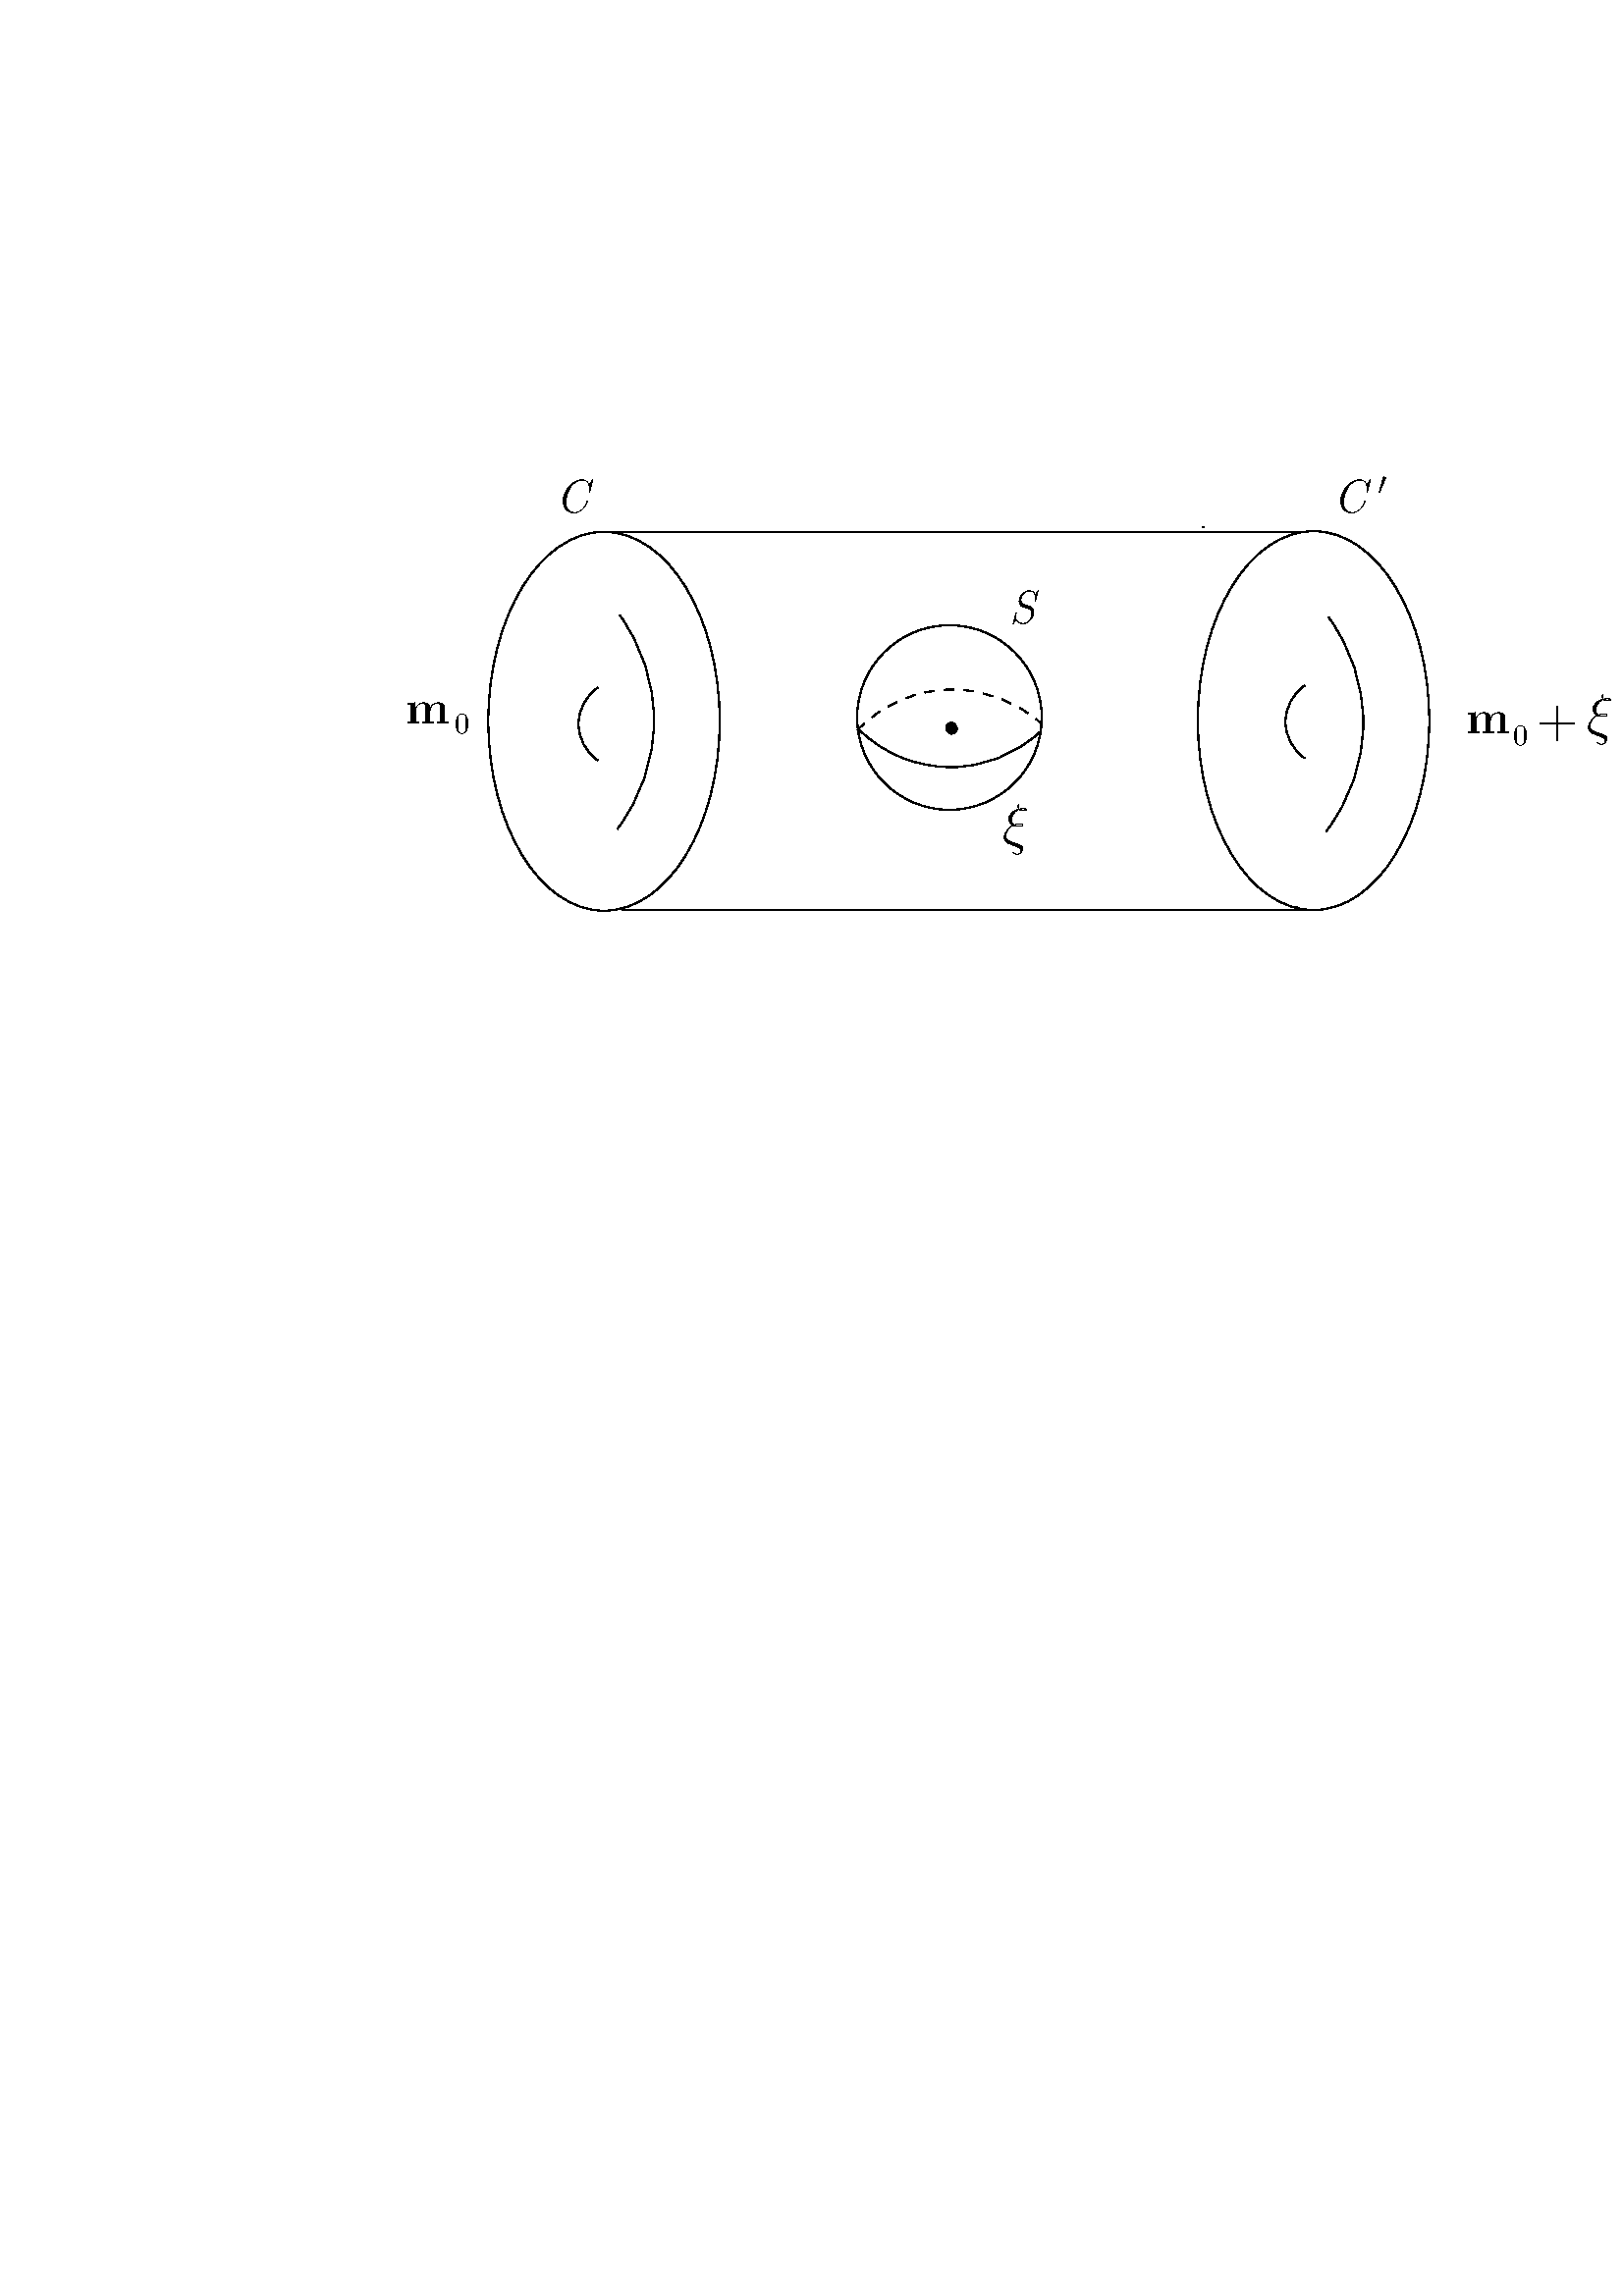
\includegraphics[width=0.75\linewidth]{figures/gla6-1.png}
\caption{插入一个 't Hooft 算子会改变 $G$-丛的拓扑，如图所示。图中画的是一个三维流形，其边界分支由两个黎曼面 $C$ 与 $C'$ 以及一个包围着 't Hooft 算子插入点的小二维球面 $S$ 组成。特征类的配边不变性意味着：若 ${\bf m}_0$ 是 $G$-丛 $E\to C$ 的特征类，则 $E\to C'$ 的特征类必为 ${\bf m}_0+\xi$，其中 $\xi=\xi({}^L\negthinspace R)$ 是与该 't Hooft 算子相联系的特征类。（原文 Fig.~11）}
\label{fig:namp}
\end{figure}
 在 $S$-对偶下，Wilson 线算子能改变离散电场 ${\bf e}_0$ 这一事实，对应着 't Hooft 线算子能改变特征类 ${\bf m}_0\in H^2(C,\pi_1(G))$ 这一事实，后者分类 $G$-丛 $E\to C$ 的拓扑。事实上，如我们在第~\ref{sec:tophooft}~节所解释的，'t Hooft 算子 $T(^L\negthinspace R)$ 是由 $S^2\cong \Bbb{CP}^1$ 上的一个 $G$-丛（可称之为 $E(^L\negthinspace R)$）构造的。这个 $G$-丛有特征类 $\xi(^L\negthinspace R)=\xi(E(^L\negthinspace R))$。't Hooft 算子对 ${\bf m}_0$ 的作用为 % 式 (8.9)
\setcounter{equation}{8}
\begin{equation}\label{eq:zuko}
{\bf m}_0\to {\bf
m}_0+\xi(^L\negthinspace R).
\end{equation}
 这个陈述是 \eqref{eq:nuko} 的 $S$-对偶，它只是来自特征类在配边下的行为，如 \namp 所示。

\begin{yizhu}[物理图像]
按：图 \ref{fig:namp} 的论证只用到特征类在配边下的不变性：三维流形的两个边界分支 $C$ 与 $C'$ 上 $G$-丛的特征类之差，等于包围 't Hooft 算子插入点的 $S^2$ 上 $G$-丛的特征类 $\xi$。这既给出式 \eqref{eq:zuko}，也解释了它为何是式 \eqref{eq:nuko} 在 $S$-对偶下的像。
\end{yizhu}

\par\medskip\emph{Wilson 算子与超对称}

让我们看看运算 \eqref{eq:yuq} 保持何种超对称。对曲线 ${\cal S}\subset \Sigma\times C$ 的一般选取，超对称 Wilson 线 $W(R,{\cal S})$ 只保持 $\MH$ 的复结构 $J$ 中的 $B$-型超对称，别的都不保持。然而，若取 ${\cal S}=\gamma\times p$，其中 $\gamma$ 是 $\Sigma$ 中的曲线、$p$ 是 $C$ 中的点，则 Wilson 算子保持更多超对称。事实上，正如我们在第~\ref{sec:lineop}~节末所证明的，它保持 $(B,B,B)$ 型超对称，即在每个复结构中都保持 $B$-型超对称。

现在我们能具体看出这一点如何反映在 Wilson 算子对膜的作用中。对点 $p\in C$，丛 ${\EUE}_p(R)$ 在 $\MH$ 的每个复结构下都是全纯的。（这可以用 $\MH$ 的超凯勒商构造自然地证明。）所以运算 \eqref{eq:yuq} 对每个复结构都保持 $B$-型超对称。

\subsection{零膜作为电特征膜}

\label{sec:zerobelectric}

现在我们可以寻找电特征膜了。考虑表示 $R$ 中、位于点 $q\in C$ 的 Wilson 线 $W_q(R)$。它把 Chan-Paton 层为 $U$ 的膜 ${\cal B}$ 映为 Chan-Paton 层为 $U\otimes {\EUE}_q(R)$ 的膜。按定义，若 $U\otimes {\EUE}_q(R)$ 与某个固定向量空间 $V$ 的 $U\otimes V$ 同构，则 ${\cal B}$ 是电特征膜。因此，条件就是：带有联络 $\Phi_q^*(\hat \CA)$ 的 ${\EUE}_q(R)$，当限制到 $U$ 的支撑集上时，必须是全纯平凡的——即同构于纤维为常数 $V$ 的向量丛。

设 $x$ 是 $\MH$ 中的一点，${\cal B}_x$ 是支撑在 $x$ 的零膜。换言之，${\cal B}_x$ 是 Chan-Paton 层为支撑在 $x$ 的天穹层 $U_x$ 的膜。我们将假定 $x$ 是 $\MH$ 的光滑点，从而可以在经典层次把场 $A_\Sigma,\phi_\Sigma$ 积掉。

任何向量丛限制到一点上都是平凡的，特别地丛 ${\EUE}_q(R)$ 限制到 $x\in \MH$ 上平凡。它到 $x$ 的限制（记作 ${\EUE}_q(R)|_x$）只是一个固定向量空间。所以
% 式 (8.10)
\setcounter{equation}{9}
\begin{equation}\label{eq:insto}
U_x\otimes {\EUE}_q(R)=U_x\otimes {\EUE}_q(R)|_x.
\end{equation}

因此，${\cal B}_x$ 是电特征膜，Wilson 圈算子 $W_q(R)$ 的「本征值」是向量空间 ${\EUE}_q(R)|_x$。

等价地，对应于零膜的 sigma 模型场边界条件说：$\cA_C$ 在 $\Sigma$ 的边界上在相差一个规范变换的意义下为常数。借助 \eqref{eq:integrout}，这意味着 ${\cal A}_\Sigma$ 在 $\Sigma$ 的边界上平凡。

我们在第~\ref{sec:lineop}~节基于底层四维拓扑场论论证过：电特征膜或磁特征膜的「本征值」必须随 $q\in C$ 变化，正如 $C$ 上平坦丛的纤维那样。确实，当 $q\in C$ 变化时，空间 ${\EUE}_q(R)|_x$ 正像平坦向量丛的纤维那样变化。事实上，取复结构 $J$，泛丛到 $x\times C$ 的限制 $({\EUE},\hat\varphi)|_x$ 给出平坦 $G_{\Bbb{C}}$ 丛 ${\EUE}|_x\to C$（因为 Hitchin 方程的解在复结构 $J$ 下对应平坦 $G_{\Bbb{C}}$-丛）。把这个丛取在表示 $R$ 中，就得到所需的平坦丛，其在 $q\in C$ 的纤维为 ${\EUE}_q(R)|_x$。我们这里选取复结构 $J$，是因为它被底层拓扑超对称特别挑出。

\begin{yizhu}[物理图像]
按：零膜的本征值虽然只是一个固定向量空间，但 $q$ 变化时它按 $C$ 上平坦丛的纤维变化；在复结构 $J$ 下这个平坦丛正是 Langlands 参数（平坦 $G_{\Bbb{C}}$ 丛）的表示版本。于是「电特征膜」同时承载了 Wilson 算子的本征值与一个局部系统——这正是几何 Langlands 对应中两侧数据会合的地方。
\end{yizhu}

在把零膜描述为电特征膜时，我们在一个关键点上稍显不正式：离散 $B$-场 ${\bf e}_0(\zeta)$ 的作用。$B$-场限制到一点上平凡，所以只要考虑零膜，就可以如我们刚才那样不正式地忽略 $B$-场。然而，更精确的描述方式如下。对每个 ${\bf e}_0$，膜范畴都包含一个对象，它是支撑在（光滑）点 $x\in \MH$ 的零膜。由于 Wilson 线算子的作用可以改变 ${\bf e}_0$，电特征膜实际上是具有不同 ${\bf e}_0$ 的扭化零膜之和（它们全都同构，因为扭化限制到一点上平凡）。对偶地，由于 't Hooft 算子可以改变 ${\bf m}_0$，磁特征膜将是支撑在 $\MH$ 不同分支上的膜之和，取遍所有可能的 ${\bf m}_0$。在几何 Langlands 纲领的标准处理中，人们说 Hecke 特征层支撑在 $\M(G,C)$ 的所有拓扑分支之并上。

\begin{yizhu}[易错点]
按：严格地说，电特征膜不是单个零膜，而是对每个 ${\bf e}_0$ 取一个在 $x$ 处的扭化零膜后作直和；这些扭化限制到点上都平凡，故彼此同构，但它们被 Wilson 算子相互联系（Wilson 算子把 ${\bf e}_0$ 平移）。对偶地，磁特征膜要对所有 ${\bf m}_0$ 分支求和，这正解释了为何 Hecke 特征层支撑在 $\M(G,C)$ 所有拓扑分支之并上，而不是单一分支上。
\end{yizhu}

\par\medskip\emph{与几何 Langlands 纲领的关系}

现在至少可以隐约看到这一切与几何 Langlands 纲领的关系。

在几何 Langlands 纲领中，人们从群 $^L\negthinspace G$ 以及同态 $\vartheta:\pi_1(C)\to{}^L\negthinspace G_{\Bbb{C}}$ 出发。（要求这个同态在第~\ref{sec:complexstr}~节所解释的某种意义下半稳定。）这样的同态构成的空间就是 Hitchin 模空间 $\MH(^L\negthinspace G,C)$。所以 $\vartheta$ 定义了 $\MH(^L\negthinspace G,C)$ 中的一点 $x(\vartheta)$。

若 $\vartheta$ 不可约，则 $x(\vartheta)$ 是光滑点，支撑在 $x(\vartheta)$ 的零膜 ${\cal B}_{x(\vartheta)}$ 是电特征膜。把 $S$-对偶作用于这个电特征膜，将得到靶为 $\MH(G,C)$ 的 sigma 模型中的磁特征膜。由第~\ref{sec:sdualhitfib}~节与第~\ref{sec:twodimint}~节可知，$\MH(^L\negthinspace G,C)$ 的零膜的 $S$-对偶是 $\MH(G,C)$ 中的膜，其支撑是 Hitchin 纤维化的一条纤维 ${\CMF}$，并配有秩一平坦 Chan-Paton 丛。我们把这样的膜称为 type ${\CMF}$ 的膜。

几何 Langlands 纲领的主要断言是：同态 $\vartheta:\pi_1(C)\to {}^L\negthinspace G_{\Bbb{C}}$ 以自然的方式联系着 $\M(G,C)$ 上的一个层，它既是 Hecke 特征层，又是完整的 ${\cal D}$-模。本文第~\ref{sec:thooftheckeop}~节至第~\ref{sec:abranes}~节将致力于解释为什么 $\MH(G,C)$ 上 type ${\CMF}$ 的膜具有正确的性质。在第~\ref{sec:thooftheckeop}~节与第~\ref{sec:bogeqheck}~节，我们把量子规范场论的 't Hooft 算子与几何 Langlands 纲领的 Hecke 算子联系起来，说明我们的磁特征膜概念如何与 Hecke 特征层的数学概念相关。在第~\ref{sec:abranes}~节，我们论证：由于 $\MH(G,C)$ 上存在某个余各向同性 $A$-膜，type ${\CMF}$ 的膜自然地联系着 $\M(G,C)$ 上微分算子的一个模。

%% ============================================================
%% 分片 22：原文第 9 节「't Hooft And Hecke Operators」（原文 glshort.tex 起于第 6755 行）
%% 由 tools/harvmac2tex.py 从 arXiv 源码（hep-th/0604151v3）自动生成。
%% 只译英文散文；公式、编号、\label、\cite 一律不改。
%% ============================================================

\section{'t Hooft 算子与 Hecke 算子}
\label{sec:thooftheckeop}

\begin{keytakeaways}
  \begin{itemize}[leftmargin=1.4em,itemsep=2pt,topsep=2pt]
    \item \textbf{物理图像}：在 $\Psi=0$（即令 $t=1$、$\theta=0$）处，四维拓扑场论在二维约化为靶空间为 Hitchin 模空间 $\MH$、复结构为 $K$ 的 $A$-模型；支撑在 $\Bbb{R}\times p$ 上的静态 't Hooft 圈算子在二维就是该 $A$-模型中的缺陷，它靠制造指定的奇点来起作用。
    \item \textbf{数学工具}：$A$-模型的经典位形是全纯映射，其态空间的经典近似是常值映射空间的上同调（在 Floer 理论中即两个拉格朗日子流形之交的上同调，需按 Maslov 指标移动维数）；四维侧用消灭定理与 Bogomolny 方程 $F=\star D\phi_0$（BPS 单极子方程）把问题化到三维。
    \item \textbf{关键结论}：静态 't Hooft 算子实现 $G$-丛的 Hecke 变换。局部写 $E=\oplus_i{\cal L}_i$ 后，算子 $T({}^L w)$ 的作用恰为 ${\cal L}_i\to{\cal L}_i\otimes{\cal O}(p_0)^{m_i}$，这正是几何 Langlands 纲领中 Hecke 修正的标准数学定义，因此 't Hooft 算子对应 Hecke 算子。
    \item \textbf{边界与展望}：本节只处理普通 Bogomolny 方程；几何 Langlands 的实际应用需要放宽时间反演对称性，改用复化（扩展）的 Bogomolny 方程，此时 't Hooft 算子给出 Hitchin 对 $(E,\varphi)$ 的 Hecke 变换，见第~\ref{sec:extbog}~节。
  \end{itemize}
\end{keytakeaways}

本节的目的是开始研究在 $\Psi=0$ 处出现的超对称 't Hooft 算子；这个取值通过令 $t=1$、$\theta=0$ 达到。主要结果将是证明：'t Hooft 算子对应于几何 Langlands 纲领中的 Hecke 算子。

我们将主要考虑静态 't Hooft 算子。于是四维流形取为 $M=\Bbb{R}\times W$，其中 $W$ 是某个三维流形；而 't Hooft 线算子将支撑在形如 $\Bbb{R}\times p$ 的一维流形上，其中 $p\in W$ 是某个点。正如我们在第~\ref{sec:loopop}~节讨论过的，这类线“算子”并不是通常意义下作用在某个预先存在的向量空间上的算子；相反，它们必须被纳入物理的、超对称的态空间的定义之中。

我们的 $\Psi=0$ 处四维拓扑场论在二维约化为靶空间为 $\MH$、复结构为 $K$ 的 $A$-模型。所以先回顾 $A$-模型的一些事实。一般地，在靶空间为 $X$ 的二维 $A$-模型中，超对称经典场位形是全纯映射 $\Phi:\Sigma\to X$。此外，超对称态空间的第一近似是 $\Sigma=\Bbb{R}\times I$ 上不依赖时间的超对称经典场所构成空间的上同调，其中 $I$ 是一个区间。超对称场就是全纯映射 $\Phi:\Sigma\to X$。但一个既全纯又不依赖时间的映射必为常值映射。所以在 $A$-模型中，物理态空间的经典近似就是满足边界条件的、到 $X$ 的常值映射所构成空间的上同调。例如在 Floer 理论中，人们取这样的边界条件：$\Bbb{R}\times I$ 的两个边界分支分别映入两个指定的拉格朗日子流形 $N,N'\subset X$。满足这些边界条件的常值映射必须把 $\Sigma$ 映入交 $N\cap N'$，于是超对称态空间的经典近似就是 $N\cap N'$ 的上同调。（必须移动上同调类的维数或鬼数（ghost number），以计入真空中被填满的费米子态数目。数学上，这个移动涉及 Maslov 指标。）

一般地，这个经典交会受到瞬子修正；对瞬子的研究正是 Floer 理论的主要内容。但我们将会看到，对于我们考虑的膜，$\Psi=0$ 处的 $A$-模型没有瞬子修正；超对称位形全都不依赖时间。

\par\medskip{\it 约化到二维}

为了约化到 $\Bbb{R}\times I$ 上的二维模型，我们特殊化迄今一直取为 $M=\Bbb{R}\times W$ 的四维流形：取 $W=I\times C$，其中 $C$ 是黎曼面，$I$ 是一个区间，并在其两端取由膜的选择所定义的边界条件。总起来说，我们在 $M=\Bbb{R}\times I\times C$ 上工作。超对称条件与第~\ref{sec:familya}~节中所见的相同：
% 式 (9.1)
\setcounter{equation}{0}
\begin{equation}\label{eq:oops}
\begin{aligned}(F-\phi\wedge\phi+tD\phi)^+ & = 0 \\
                      (F-\phi\wedge\phi-t^{-1}D\phi)^-& = 0 \\
                      D^* \phi & = 0.\\\end{aligned}
\end{equation}

在 $t=1$（研究 't Hooft 算子时我们通常作此假设）时，\eqref{eq:oops}\ 的前两个方程可写为 $F-\phi\wedge \phi+\star D\phi=0$。用复联络 $\CA=A+i\phi$ 及其曲率 $\CF=d\CA+\CA\wedge\CA$ 表示，这等价于 % 式 (9.2)
\setcounter{equation}{1}
\begin{equation}\label{eq:nops}
{\cal F}+i\star\bar\CF=0.
\end{equation}

在没有 't Hooft 圈、并取适当边界条件时，与第~\ref{sec:vanishing}~节类似的消灭定理表明：这些方程在 $M=\Bbb{R}\times I\times C$ 上的解是从 $C$ 拉回的，并且来自 $\Sigma=\Bbb{R}\times I$ 到 $\MH$ 的常值映射。这是四维拓扑场论约化为二维 sigma 模型的一部分。

\begin{figure}[htbp]
\centering
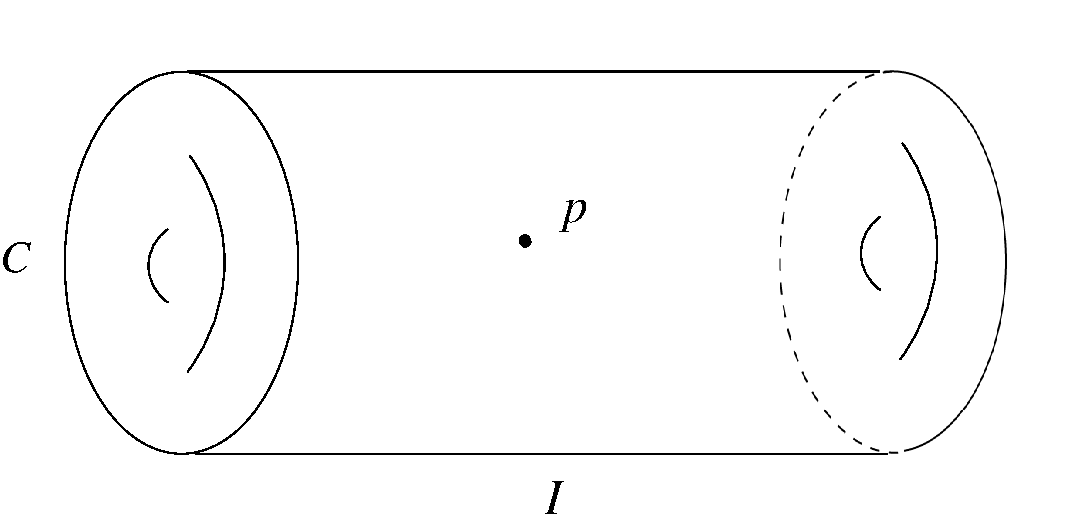
\includegraphics[width=0.75\linewidth]{figures/gla7-1.png}
\caption{插在 $I\times C$ 中点 $p=y\times p_0$ 处的静态 't Hooft 线。在该点附近，Bogomolny 方程的解具有指定的奇点。（原文 Fig.~12）}
\label{fig:botampo}
\end{figure}

把 't Hooft 线包含进来后，事情变得更复杂（\botampo）。如我们从第~\ref{sec:tophooft}~节回忆的那样，'t Hooft 算子在经典场位形中制造指定的奇点。对于支撑在直线 $\Bbb{R}\times p$ 上的 't Hooft 算子（其中 $p\in I\times C$），奇点将妨碍我们证明解是从 $C$ 拉回的。但对某些边界条件，仍有一个较弱的消灭结果成立：\eqref{eq:oops}\ 的相关解不依赖时间，即在对 $\Bbb{R}$ 的平移下不变。

为解释这一点，回忆一下：从几何 Langlands 对偶的观点看，最重要的 $A$-膜是 type ${\CMF}$ 的膜，它们支撑在 Hitchin 纤维化的一个纤维上，并带秩 1 的平坦 Chan-Paton 丛。它们是零膜的 $S$-对偶，因此预期是磁特征膜。正如第~\ref{sec:mhbranes}~节所解释的，它们是 $(B,A,A)$ 型膜，即相应的边界条件与两个线性无关的拓扑超荷相容，而这两个超荷的适当线性组合生成复结构 $I$ 中 $B$-模型的拓扑超对称，以及复结构 $J$ 和 $K$ 中 $A$-模型的拓扑超对称。

当我们考虑具有 $(B,A,A)$ 边界条件并插入 't Hooft 算子的 BRST 不变场位形时，可以区分两类位形：保持两个费米对称性的位形，以及只保持复结构 $K$ 中 $A$-型超对称的位形。在后一情形，破缺的超对称产生一个额外的费米零模；由于它由一个对称性生成，不会被量子修正消除，从而阻止这类瞬子对任何拓扑可观测量作出贡献。（也可能存在其他费米零模，其存在性并不来自费米对称性。）因此，感兴趣的贡献只来自同时保持两个超对称的瞬子。

事实上，具备所需性质的瞬子不依赖时间。从 sigma 模型即可猜到此点，因为复结构 $I$ 中的 $B$-模型没有非平凡瞬子。在 $\Bbb{R}\times I\times C$ 上完整扭化超对称规范场论的框架中，即使存在静态 't Hooft 算子，该结论也成立。最一般的证明涉及 moment map 论证，将另文给出 \cite{ref26}。这里我们概述另一个论证，它对最重要的 $(B,A,A)$-膜（例如 ${\CMF}$ 型膜）已经足够。

首先我们需要一个关于 $\phi_1$ 的消灭定理，$\phi_1$ 是 $\phi$ 在 $M=\Bbb{R}\times I\times C$ 的 $I$ 方向上的分量。在任何一个经典瞬子解中，$\phi_1$ 满足它自己的二阶 Euler-Lagrange 方程，这些方程可由经典作用量 \eqref{eq:nuseful}\ 推出，其形式为 % [WARN] 公式 \eqn\eqref{eq:zungo} 无编号或重复
\begin{equation*}
\tag*{(9.3)}
-D_\mu
D^\mu\phi_1+[\phi_\mu,[\phi_1,\phi^\mu]]=0.
\end{equation*}
 我们假设 $\phi_1$ 在每个膜上满足 Dirichlet 或 Neumann 边界条件；对最重要的那些膜这是成立的。用 $\phi_1$ 乘该方程、取迹并在时空上积分，得到
% 式 (9.4)
\setcounter{equation}{3}
\begin{equation}\label{eq:wungo}
\int d^4x\ \Tr\left( D_\mu\phi_1
D^\mu\phi_1+[\phi_1,\phi_\mu][\phi_1,\phi^\mu]\right)=0.
\end{equation}

分部积分不产生边界项，因为已假定了边界条件；而且 't Hooft 算子带来的奇点也不成问题，因为 $\phi_1$ 在静态 't Hooft 算子附近非奇异。由于被积式是负定的，上述恒等式蕴含 $D_\mu\phi_1=[\phi_\mu,\phi_1]=0$，从而在解不可约的情形下 $\phi_1=0$。

在这个论证中，我们默认分部积分在遥远的过去或未来不产生边界项。我们并不能先验地知道方程的超对称解不依赖时间。然而，我们至少假设所需的解在遥远的过去或未来趋近于不依赖时间的“真空”解。先对时间无关的情形运行上一段的论证，便可得知每个真空中 $\phi_1=0$。于是，由于 $W$ 紧，$\phi$ 在遥远的过去或未来以指数速度趋于 0。因此，上一段用来证明处处 $\phi_1=0$ 的分部积分中没有边界项。

现在我们要证明：一个既具有复结构 $J$ 中又具有复结构 $K$ 中 $A$-模型的拓扑超对称、并且满足 $\phi_1=0$ 的场，实际上不依赖时间。复结构 $K$ 中 $A$-模型的超对称方程就是 $t=1$ 时的方程 \eqref{eq:oops}；复结构 $J$ 中 $A$-模型的方程则由此作一个 ${\cal U}_1$ 变换 $\varphi\to i\varphi$ 得到。把 $M=\Bbb{R}\times I\times C$ 上合并后的方程组写出来，并证明若再加上 $\phi_1=0$，它们便蕴含场在规范变换下不依赖时间，这是一个小练习。

不依赖时间的超对称场可以在 $M=\Bbb{R}\times W$ 连同静态 Wilson 线的更一般框架中方便地分析（不必特殊化到 $W=I\times C$），尽管我们关于所有相关超对称场都不依赖时间的论证在这种一般性下并不成立。当特殊化到 $M=\Bbb{R}\times W$ 时，还有时间反演不变性这一额外对称性 ${\EUT}$，它作用为 $s\to -s$，其中 $s$ 是 $\Bbb{R}$ 上的“时间”坐标；${\EUT}$ 在 $W$ 上平凡作用，并把 $(A,\phi)\to ({\EUT}^*A,-{\EUT}^*\phi)$。（这是第~\ref{sec:canonpar}~节末尾讨论的定向反转对称性的一个例子。）$\phi$ 的符号改变是必要的，因为 ${\EUT}$ 反转向 \eqref{eq:nops} 中 Hodge $\star$ 算子的符号。

因此，我们可以一致地只考虑既不依赖时间又 ${\EUT}$ 不变的解。在这样的解中，$G$-丛 $E$ 与联络 $A$ 是从 $W$ 拉回的。此外，$\phi$ 取形式 $\phi_0\,ds$，其中 $\phi_0$ 是 $W$ 上取值于 ${\rm ad}(E)$ 的零形式。方程约化为
% 式 (9.5)
\setcounter{equation}{4}
\begin{equation}\label{eq:bogeq}
F=\star D\phi_0.
\end{equation}
 我们的定向约定使四维中 $\star(dx^0\wedge dx^1)=dx^2\wedge dx^3$，三维中 $\star(dx^1)=dx^2\wedge dx^3$。方程 \eqref{eq:bogeq}\ 是标准的 Bogomolny 方程 \cite{ref105}，描述超对称或 BPS 单极子\footnote{这个名称反映了这样一个事实：基本的超对称单极子解也在 \cite{ref106} 中作为二阶 Yang-Mills-Higgs 方程的解被发现。}，并且已得到广泛研究，例如 
\cite{ref107,ref108,ref109}。得到 Bogomolny 方程的更熟悉的方式，是寻找 $\Bbb{R}^4$ 上沿某一方向平移不变的 Yang-Mills 瞬子方程的解。

本节中，我们将首先在普通 Bogomolny 方程 \eqref{eq:bogeq} 的框架下分析静态 't Hooft 算子。我们将证明它们实现 $G$-丛的 Hecke 变换，也就是几何 Langlands 纲领中通常定义的 Hecke 变换（Hecke transformation）。这将涉及研究带有由 't Hooft 算子造成的点奇点的 BPS 单极子解。Bogomolny 方程的这种奇异解最早由 Kronheimer 在未发表的工作 \cite{ref110} 中研究过。它们可以作为更大规范群的光滑单极子解的极限出现 
\cite{ref111,ref112,ref113,ref114}，也可来自某些弦论膜位形 \cite{ref115}，后者启发了更晚近的研究 
\cite{ref116,ref117,ref118}。然后我们将对 $G$-丛的 Hecke 修正作一个初等的介绍——从数学观点看既不声称新颖、也不声称完备！

在第~\ref{sec:extbog}~节中，我们将推广这一分析，放宽时间反演对称性的假设。我们将会看到，在这种情形下，超对称方程给出 Bogomolny 方程的一种复化或扩展的类似物，它似乎尚未被研究过。在这些扩展方程的框架中，静态 't Hooft 算子通过 Higgs 丛（换言之，Hitchin 对 $(E,\varphi)$）的 Hecke 变换起作用。这种扩展意义上的 Hecke 算子在数学上是自然的，并且此前已被考虑过 
\cite{ref119,ref120}。

几何 Langlands 纲领中的应用实际上依赖于扩展的 Bogomolny 方程与扩展的 Hecke 算子。只有当边界条件（即膜的选择）保证 Higgs 场 $\varphi$ 消失时，我们才能退回到普通的 Bogomolny 方程与 Hecke 算子。典型应用并非这种情形。不过，我们从普通的 Bogomolny 方程与 Hecke 算子讲起，并把大部分注意力放在它们上面，因为这种情形更简单，且能展示主要思想。

\begin{yizhu}[原文疑误]
式 (9.4) 下方原文称被积式是“负定的”（negative-definite），译文照原文译作负定。按：$M=\Bbb{R}\times I\times C$ 是黎曼流形，在 $\Tr$ 下 $D_\mu\phi_1D^\mu\phi_1$ 是半正定的，而 $[\phi_1,\phi_\mu][\phi_1,\phi^\mu]$ 的迹也非负（因 $[\phi_1,\phi_\mu]$ 反厄米，其平方取迹为负），故该被积式应为半正定；原文用“负定”多半是沿用了把作用量写成 $-\int\Tr(\cdots)$ 的符号约定。结论 $D_\mu\phi_1=[\phi_\mu,\phi_1]=0$ 不受影响。
\end{yizhu}

\begin{yizhu}[易错点]
$t=1$ 时式 (9.1) 的前两式为何合并为 $F-\phi\wedge\phi+\star D\phi=0$：记 $X=F-\phi\wedge\phi$。四维中 $\star$ 把自对偶 2-形式映为反自对偶、反之亦然，且 $\star^2=1$，故 $X\pm\star D\phi=0$ 的自对偶部分为 $X^+ +(D\phi)^+$、反自对偶部分为 $X^--(D\phi)^-$；而 $(D\phi)^\pm$ 正是 $D\phi$ 的（反）自对偶投影。于是 $X+\star D\phi=0$ 恰好同时等价于 $(X+D\phi)^+=0$ 与 $(X-D\phi)^-=0$，即式 (9.1) 在 $t=1$ 的前两式。按：这一步是后文把超对称条件写成复联络方程 (9.2) 的关键，读 (9.2) 时须记住 $\CA=A+i\phi$ 的虚部就是 Higgs 场（在复结构 $I$ 中）。
\end{yizhu}

\begin{yizhu}[易错点]
式 (9.5) 前后的定向约定：原文取四维 $\star(dx^0\wedge dx^1)=dx^2\wedge dx^3$，三维 $\star(dx^1)=dx^2\wedge dx^3$。这里 $s=x^0$ 是 $\Bbb{R}$ 上坐标，$x^1$ 是 $W$ 上坐标；两个式子的相容性在于 Hodge 星对分解 $M=\Bbb{R}\times W$ 满足 $\star_4(ds\wedge\alpha)=\star_3\alpha$。由于 $\phi=\phi_0\,ds$ 是沿 $ds$ 的 1-形式，$D\phi$ 与 $F$ 都是 2-形式，式 (9.5) 中出现的 $\star$ 实际是 $W$ 上的三维 $\star$（作用在 $W$ 的 2-形式上）。按：若把这里的 $\star$ 误当成四维 $\star$，会多出 $ds$ 因子，方程 (9.5) 就不成立了。
\end{yizhu}

\begin{yizhu}[易错点]
时间反演 ${\EUT}$ 为何要令 $\phi$ 变号：$s\to -s$ 反转 $M=\Bbb{R}\times W$ 的定向，从而 $\star\to -\star$，方程 (9.2) ${\cal F}+i\star\bar\CF=0$ 不再保持原形。若同时把 $\CA=A+i\phi$ 换成其复共轭 $\bar\CA=A-i\phi$（即 $\phi\to-\phi$），则 ${\cal F}\leftrightarrow\bar\CF$，方程化为原方程的共轭式，仍然成立。按：原文把这条变换放在“定向反转对称性”的一般框架下（第~\ref{sec:canonpar}~节末），$\phi$ 是 1-形式，其时间分量在此变换下的行为正是 $\phi_0\,ds$ 中 $ds$ 被反转、再整体补一个负号的结果；后文推 (9.5) 时用的就是这个不变性。
\end{yizhu}

\begin{yizhu}[物理图像]
为什么 $\Psi=0$ 处“没有瞬子修正”、超对称位形都不依赖时间：在 $(B,A,A)$ 型边界条件下，$B$-模型（复结构 $I$）部分没有非平凡瞬子（$I$ 中 $B$-模型的态空间经典近似即常值映射上同调），而 $A$-模型（复结构 $J,K$）部分的瞬子若只保持一个超荷，就会产生不被量子修正消除的费米零模，从而对拓扑可观测量无贡献；因此有贡献的瞬子必须同时保持两个超荷，而这类位形可证不依赖时间。参见 Witten 2008 综述关于 B-模型/A-模型与 Hitchin 纤维化的讨论。按：这正是本节能把四维问题约化为三维 Bogomolny 方程的依据；一旦放宽时间反演假设（下节），就会出现扩展 Bogomolny 方程。
\end{yizhu}

\begin{yizhu}[易错点]
本片沿用的 harvmac 记号不要展开或改名：${\CMF}$ 是 $\mathbf{F}$（Hitchin 纤维化的典型纤维），不是普通的 $\cal F$；$\botampo$、$\otampo$、$\notampo$ 分别展开为 “fig.~12/13/14”（原文图号，见 macros.tex），与 \verb|\ref| 不同，不要替换成 \verb|\ref{fig:...}|；${\EUT}$ 是时间反演对称性、${\EUN}$ 是 $\cal N$。此外“鬼数（ghost number）”的移动就是按填入的费米子态数平移上同调的次数，与 Maslov 指标在 Floer 理论中的作用相同。
\end{yizhu}

%% ============================================================
%% 分片 23：原文第 9 节「't Hooft And Hecke Operators」（原文 glshort.tex 起于第 6755 行）
%% 由 tools/harvmac2tex.py 从 arXiv 源码（hep-th/0604151v3）自动生成。
%% 只译英文散文；公式、编号、\label、\cite 一律不改。
%% ============================================================

\subsection{'t Hooft 算子与 Hecke 修正}

\label{sec:theck}

先考虑 $W=\Bbb{R}^3$ 上的 Bogomolny 方程，我们把 $\Bbb{R}^3$ 看作 $\Bbb{R}\times\Bbb{C}$，其中 $\Bbb{C}$ 用 $z=x^2+ix^3$ 参数化，$\Bbb{R}$ 用 $y=x^1$ 参数化。我们有 % 式 (9.6)
\setcounter{equation}{5}
\begin{equation}\label{eq:boffo}
\begin{aligned}\star dy&={i\over 2}dz\wedge
d\bar z\\
        \star dz&=-idz\wedge dy\\
        \star d\bar z& = id\bar z\wedge dy.\\\end{aligned}
\end{equation}

把 $F=dz\wedge d\bar z \,F_{z\bar z}+dy\wedge dz
        F_{yz}+dy\wedge d\bar z F_{y\bar z}$ 展开（同样地展开
$D\phi_0=dy D_y\phi_0+dz D_z\phi_0+d\bar z D_{\bar z}\phi_0$），
Bogomolny 方程变为 % 式 (9.7)
\setcounter{equation}{6}
\begin{equation}\label{eq:noffo}
\begin{aligned}F_{z\bar
z}&={i\over 2}D_y\phi_0\\
                    F_{yz}&=iD_z\phi_0\\
                    F_{y\bar z}&=-iD_{\bar z}\phi_0.\\\end{aligned}
\end{equation}

更一般地，取 $W= \Bbb{R}\times C$，其中 $C$ 是黎曼面。用 $z$ 记 $C$ 上的局部复坐标，给 $C$ 配上 Kähler 度量 $h(z,\bar z)|dz|^2$（$h$ 为某正函数），并取 $W$ 上的度量为 $h(z,\bar
z)|dz|^2+dy^2$。\eqref{eq:boffo}\ 与 \eqref{eq:noffo}\ 中的第一式分别变为 % 式 (9.8)
\setcounter{equation}{7}
\begin{equation}\label{eq:jungol}
\begin{aligned}\star dy& ={ih\over 2}\,dz\wedge
d\bar z\\ F_{z\bar z}&={ih\over 2}D_y\phi_0.\end{aligned}
\end{equation}
 其余
方程不变。

复维数为 1 时，$\bar\partial $ 算子没有可积性条件。因此 $G$-丛
$E\to C$ 上的任何联络 $A$ 都给 $E$ 赋予一个全纯结构。我们只需
把 $\bar \partial$ 算子定义为 $\bar D=d\bar z D_{\bar
z}=d\bar z(\partial_{\bar z}+A_{\bar z})$。

\begin{figure}[htbp]
\centering
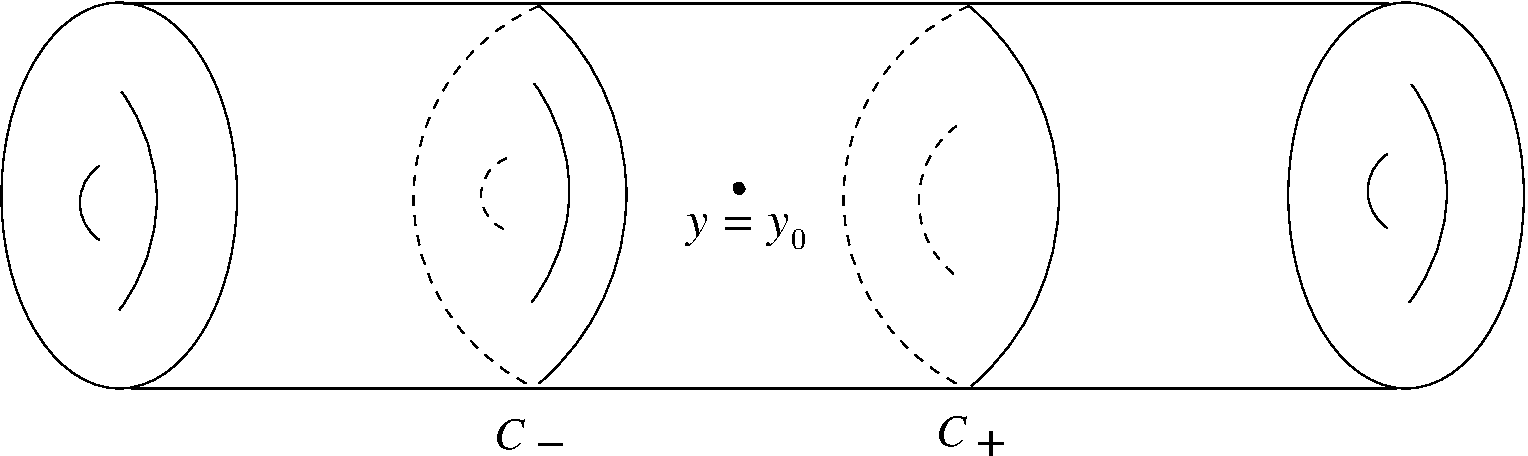
\includegraphics[width=0.75\linewidth]{figures/gla7-2.png}
\caption{在 $G$-丛 $E$ 上 Bogomolny 方程的解中，$E_y$（即 $E$ 到 $\{y\}\times C$ 的限制）的全纯型是常数，除非越过某个 't Hooft 算子的位置。图中画出了位于 $y=y_0$ 的 't Hooft 算子，以及 $y_0$ 左右两侧的 $C_y=\{y\}\times C$ 的一些拷贝，分别记作 $C_-$ 与 $C_+$。（原文 Fig.~13）}
\label{fig:otampo}
\end{figure}

于是，当 $y$ 在 $ \Bbb{R}$ 中变动时，$G$-丛 $E\to  \Bbb{R}\times C$ 上的任何联络 $A$ 都定义了一族全纯 $G$-丛 $E_y\to C$。$E_y$ 就是 $E$ 到 $C_y= \{y\}\times C$ 的限制（\otampo）。现在假设 $A$ 满足 Bogomolny 方程。让我们在规范 $A_y=0$ 中工作。此时 $F_{y\bar z}=\partial_yA_{\bar z}$。因此 \eqref{eq:noffo}\ 中的最后一个方程告诉我们 % 式 (9.9)
\setcounter{equation}{8}
\begin{equation}\label{eq:troffo}
{\partial\over
\partial y}A_{\bar z}=-iD_{\bar z}\phi_0.
\end{equation}

但右端是 $A_{\bar z}$ 在由 $-i\phi_0$ 生成的规范变换下的变化。因此 $E_y$ 的全纯型与 $y$ 无关。（陈述这个论证的另一种方式是注意到 $\partial_y\bar D=-i[\bar D,\phi_0]$，这表明 $\bar D$ 在共轭意义下与 $y$ 无关。）

现在来看看，若在 $\Bbb{R}\times C$ 中的点 $p=y_0\times p_0$ 处加入一个 't Hooft 算子会发生什么。这意味着我们考虑定义在点 $p$ 的补集上、并在 $p$ 附近具有某种类型奇点的丛 $E$ 与联络 $A$，如第~\ref{sec:tophooft}~节所述。

在 $y=y_0$ 之外，上述论证适用，$E_y$ 的全纯型与 $y$ 无关。在 $y=y_0$ 处，由于奇点，丛 $E_y$ 没有定义。越过 $y=y_0$ 时，丛的全纯型可能跳跃。然而，它只能以非常特殊的方式跳跃。若把 $E$ 限制到 $C\backslash p_0$（即 $p_0$ 在 $C$ 中的补集），则上述论证适用，限制后的丛 $E_y$ 的全纯型即使在 $y=y_0$ 处也是常数。所以 $E_y$ 的全纯型可以在 $y=y_0$ 处跳跃，但只能以一种在从 $C$ 中删去点 $p_0$ 后便成为平凡的方式跳跃。

下面我们试图精确描述 $E_y$ 在 $y=y_0$ 处可以如何跳跃。先考虑阿贝尔情形，再考虑非阿贝尔情形。

\par\medskip{\it 阿贝尔情形}

从 $G=U(1)$ 开始。此时 $E$ 是复线丛 ${\cal L}$。把 $y<y_0$ 时的 ${\cal L}_y$ 记为 ${\cal L}_-$，把 $y>y_0$ 时的 ${\cal L}_y$ 记为 ${\cal L}_+$。线丛 ${\cal L}_-$ 与 ${\cal L}_+$ 在点 $p_0\in C$ 的补集上同构。

这意味着线丛 ${\cal L}_+\otimes {\cal L}_-^{-1}$ 在 $p_0$ 之外平凡。于是它有截面 $s$，该截面在 $p_0$ 之外既无零点也无极点；令 $q$ 为其在 $p_0$ 处零点的阶数。则 ${\cal L}_+\otimes {\cal L}_-^{-1}\cong {\cal O}(p_0)^q$。这里照例 ${\cal O}(p_0)$ 是这样一个线丛：其全纯截面是 $p_0$ 之外全纯、在 $p_0$ 处至多有一个单极点的函数。于是 ${\cal L}_+$ 与 ${\cal L}_-$ 的关系为 ${\cal L}_+\cong {\cal L}_-\otimes {\cal O}(p_0)^q$，其中 $q$ 为某个整数。

我们回忆一下，群 $G=U(1)$ 的 't Hooft 算子 $T(m)$ 由整数 $m$ 的选择来分类。（若要指明点 $p_0$，我们把它写成 $T(m;p_0)$。）这提示了一个显然的猜想：$m$ 可能就等于上一段中的整数 $q$。

算子 $T(m)$ 的定义是：在 $p=p_0\times y_0$ 附近，曲率具有奇异行为 % 式 (9.10)
\setcounter{equation}{9}
\begin{equation}\label{eq:formigo}
F\sim
\star d\left({im\over 2}{1\over |\vec x - p|}\right),
\end{equation}
 其中
$|\vec x-p|$ 是 $p$ 到附近点 $\vec x\in
 \Bbb{R}\times C$ 的距离。这意味着，若 $S$ 是如图中那样包围点 $p$ 的小球面，则 $\int_S c_1({\cal L})=m$。因此 't Hooft 算子 $T(m)$ 彼此在拓扑上都是不同的。这个论断（若 $G$ 非阿贝尔则远不成立）将使我们在阿贝尔情形下仅凭拓扑理由就确定 $T(m)$ 的作用。

\begin{figure}[htbp]
\centering
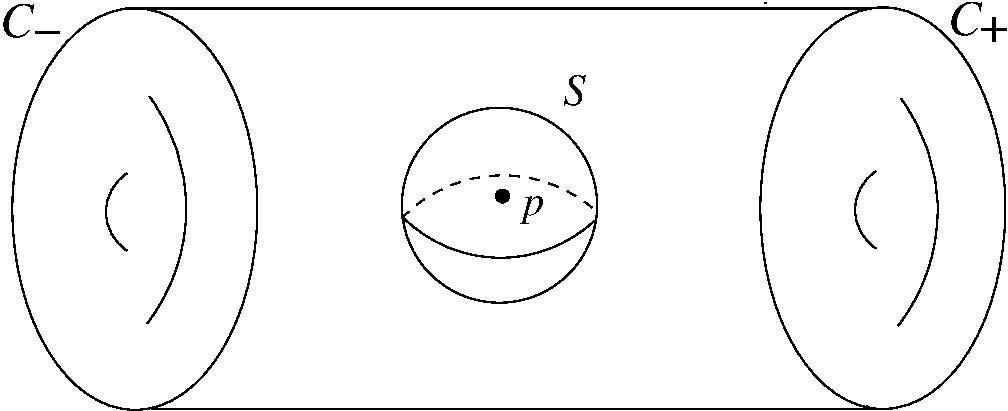
\includegraphics[width=0.75\linewidth]{figures/gla7-3.png}
\caption{二维闭链 $C_-+S$ 与 $C_+$ 之间的一个配边（cobordism），表明同调闭链 $D=C_+-C_--S$ 是一个边界。（原文 Fig.~14）}
\label{fig:notampo}
\end{figure}

 现在取满足 $y_-<y_0<y_+$ 的 $y_\pm$，把 $y_\pm\times C$ 记为 $C_\pm$，于是 ${\cal L}_\pm $ 是 ${\cal L}$ 到 $C_\pm$ 的限制。令 $q_\pm=\int_{C_\pm}c_1({\cal L})$。按 \notampo 中那样显然的定向选择，同调闭链 $D=C_+-C_--S$ 是 $(\Bbb{R}\times C)\backslash p$ 中的一个边界。因此 $0=\int_Dc_1({\cal L})=\int_{C_+}c_1({\cal L})-\int_{C_-}c_1({\cal L})-\int_Sc_1({\cal L})=q_+-m-q_-$。

所以 $q_+=m+q_-$。因此，在 $p_0$ 之外同构的 ${\cal L}_+$ 与 ${\cal L}_-$，其第一 Chern 类相差 $m$。于是 ${\cal L}_+\cong {\cal L}_-\otimes {\cal O}(p_0)^m$。

这样，我们就确定了 $G=U(1)$ 时 't Hooft 算子的作用。't Hooft 算子 $T(m;p_0)$，即在点 $p_0\in C$ 处插入的算子 $T(m)$，通过用 ${\cal O}(p_0)^m$ 扭化来作用。这个结果与 $U(1)$ 的 Hecke 算子的标准定义一致。

我们看到，与第~\ref{sec:lineop}~节的一般论证一致，插入在 $C$ 中不同点处的 't Hooft 算子彼此对易。此外，给定点 $p_0\in C$ 处的 't Hooft 算子构成一个交换群，满足 $T(m;p_0)=T(1;p_0)^m$。

\par\medskip{\it 非阿贝尔情形：$U(N)$}

现在讨论非阿贝尔情形中 't Hooft 算子的作用。先考虑群 $U(N)$。有两件事使这个群易于分析：$U(N)$ 有一个方便的表示，即我们记作 $\VV$ 的 $N$ 维表示；并且 $U(N)$ 是它自己的 Langlands 对偶。

't Hooft 算子的定义依赖于同态 $\rho:U(1)\to U(N)$ 的选择（模共轭）。最一般的这种同态把 $\exp({i\alpha})\in U(1)$ 映为对角矩阵 ${\rm
diag}(\exp({im_1\alpha}),\exp({im_2\alpha}),\dots,
\exp({im_N\alpha}))$，其中整数 $N$ 元组
$^L\negthinspace w=(m_1,m_2,\dots,m_N)$ 在置换意义下唯一。（我们把这个量记作 $^L\negthinspace w$，因为在一般情形下它将是 Langlands 对偶群 $^L\negthinspace G$ 的一个权。）我们通常把 $m_i$ 排序使 $m_1\geq
m_2\geq \dots\geq m_N$。在 Lie 代数层面，$\rho$ 把 $1\in \frak{u}(1)$ 映为对角矩阵
% 式 (9.11)
\setcounter{equation}{10}
\begin{equation}\label{eq:morphy}
\left(\begin{matrix}m_1& & & \dots & \\
                                    &m_2& & \dots & \\
                          & & m_3 &\dots & \\
                & & \vdots & \dots& \\
            & & & & m_N\\\end{matrix}\right).
\end{equation}

相应的 't Hooft 算子 $T(^L\negthinspace w)$ 的定义是：在点 $p\in  \Bbb{R}\times C$ 附近，规范场具有把基本 $U(1)$ 奇点通过该嵌入映入 $U(N)$ 所得的奇点。例如，$p$ 附近曲率的奇异部分为对角的
% 式 (9.12)
\setcounter{equation}{11}
\begin{equation}\label{eq:orphy}
F\sim \star d\left({i\over 2}{1\over |\vec x -
p|}\right) \left(\begin{matrix}m_1& & & \dots & \\
                                    & m_2& & \dots & \\
                          & & m_3 &\dots & \\
                & & \vdots & \dots& \\
            & & & & m_N\\\end{matrix}\right).
\end{equation}

在 $p$ 附近，Bogomolny 方程约化为 $U(N)$ 的某个极大环面 ${\cal T}=U(1)^N$ 中的方程。（从全纯观点看，更自然的做法是考虑相应的、约化到规范群复化中的复化极大环面的方程，即约化到 $U(N)_{\Bbb{C}}=GL(N,\Bbb{C})$。）与方程约化到极大环面相应，丛 $E_y$ 在 $p_0\times y \in C_y$ 附近分裂为线丛之和 ${\cal L}_1\oplus {\cal L}_2\oplus\dots \oplus {\cal L}_N$（它们每一个当然都在 $p$ 附近平凡）。't Hooft 算子对 ${\cal L}_i$ 的作用恰与阿贝尔情形相同，即 ${\cal L}_i\to {\cal L}_i\otimes {\cal O}(p_0)^{m_i}$。

这样，我们就得到了 't Hooft 算子 $T(^L\negthinspace w)$ 在丛 $E$ 上如何作用的描述。相对于 $E$ 在 $p$ 附近作为 $\oplus_{i=1}^N{\cal L}_i$ 的某个分解，它通过 ${\cal L}_i\to {\cal L}_i\otimes {\cal O}(p_0)^{m_i}$ 作用。这与 $U(N)$ 的 Hecke 算子作用的通常数学描述一致。这就是 't Hooft 算子与 Hecke 算子之间的基本联系。

在第~\ref{sec:spaceheck}~节 与 第~\ref{sec:affgrass}~节中，我们将讨论 $E$ 的局部分解 $E=\oplus_{i=1}^N{\cal L}_i$ 中包含何种数据，以及其中多少数据与 't Hooft 算子的作用相关。这个问题的通常答案涉及所谓仿射 Grassmann 流形，我们将在第~\ref{sec:affgrass}~节中简要描述。

\par\medskip{\it 若干例子}

一般地，正如我们从第~\ref{sec:tophooft}~节所知，Langlands 对偶群 $^L\negthinspace G$ 的表示自然地对应于 $G$ 的 't Hooft 算子。最高权为 $^L\negthinspace w$ 的表示 $R(^L\negthinspace w)$ 对应于一个 't Hooft 算子，我们把它写作 $T(R(^L\negthinspace w))$，或简记为 $T(^L\negthinspace w)$。在当前的讨论中，$^L\negthinspace G=G=U(N)$。

例如，$U(N)$ 的基本 $N$ 维表示 $\VV$ 在我们约定 $m_1\geq m_2\geq \dots\geq m_N$ 下的最高权为 $^L\negthinspace w(1)=(1,0,0,\dots,0)$，它对应于 't Hooft 算子 $T(^L\negthinspace w(1))$，或简记为 $T_{(1)}$。对 $k=1,\dots,N$，第 $k$ 个反对称张量表示 $\wedge^k\VV$ 的最高权为 % 式 (9.13)
\setcounter{equation}{12}
\begin{equation}\label{eq:nyto}
^L\negthinspace
w(k)=(\overbrace{1,1,\dots,1}^{\text {$k$ times}},0,\dots,0)
\end{equation}
 并
对应于 't Hooft 算子 $T_{(k)}$。

表示 $\wedge^N\VV$ 是一维的；它是 $g\in U(N)$ 通过乘以 $\det(g)$ 作用的表示。它可以提升到任意整数幂 $u$（正或负），得到 $g$ 通过 $(\det(g))^u$ 作用的表示。这个表示我们记作 $(\wedge^N\VV)^u$，它对应于权 $^L\negthinspace w=(u,u,\dots,u)$。对应于 $\wedge^N\VV$ 的 't Hooft/Hecke 算子 $T_{(N)}$ 简单地通过 $E\to E\otimes {\cal O}(p_0)$ 作用（如同阿贝尔情形），并且显然是可逆的。它的 $u$ 次幂对应于表示 $(\wedge^N\VV)^u$。而 $k<N$ 的 $T_{(k)}$ 不可逆。

$U(N)$ 的中心元素 $\exp(i\alpha)$ 在表示 $\wedge^k\VV$ 上通过乘以 $\exp(ik\alpha)$ 作用。更一般地，它在最高权为 $^L\negthinspace w=(m_1,m_2,\dots,m_N)$ 的任何表示上通过乘以 $\exp(i\alpha\sum_{i=1}^Nm_i)$ 作用。这个陈述的一个特例是：$U(N)$ 的中心平凡作用当且仅当 % 式 (9.14)
\setcounter{equation}{13}
\begin{equation}\label{eq:hoty}
\sum_im_i=0.
\end{equation}
 $S$-对偶，正如我们在第~\ref{sec:electricbranes}~节讨论过的，把 $^L\negthinspace G$ 的中心在表示 $^L\negthinspace R$ 上的作用，映为相应的 't Hooft 算子 $T(^L\negthinspace R)$ 对 $G$-丛拓扑的作用。确实，由于 $T(^L\negthinspace w)$ 局部把 $\oplus_i{\cal L}_i$ 映为 $\oplus_i\left({\cal L}_i\otimes {\cal O}(p_0)^{m_i}\right)$，它把 $c_1(E)$ 改变为 % [WARN] 公式 \eqn\eqref{eq:yorgo} 无编号或重复
\begin{equation*}
\tag*{(9.15)}
c_1(E)\to c_1(E)+\sum_im_i,
\end{equation*}
 于是
$E$ 的拓扑不变当且仅当 $\sum_im_i=0$。

由 $S$-对偶，我们预期 $G$ 的 't Hooft 算子构成一个交换代数，同构于 $^L\negthinspace G$ 的表示环。（事实上，正如我们在第~\ref{sec:lineop}~节讨论过的，'t Hooft 算子的对易性可由四维拓扑场论的更一般考虑得出，而不必借助 $S$-对偶。）我们将在第~\ref{sec:kahstr}~节 从 Bogomolny 方程的角度考察这一点。$U(N)$ 的表示环由表示 $\wedge ^k\VV,\,k=1,\dots,N$ 连同 $(\wedge^N\VV)^{-1}$ 自由生成。相应地，$U(N)$ 的 't Hooft 算子构成的交换代数由 $T_{(k)}$ 连同 $T_{(N)}^{-1}$ 自由生成。在几何 Langlands 纲领的数学文献中，这些生成元通常被取作 $U(N)$ 的基本 Hecke 运算。

\par\medskip{\it 其他群的 't Hooft/Hecke 算子}

把这一切推广到任意紧规范群 $G$ 相当直接。为使讨论相对简单，我们取 $G$ 的一个表示 $R$，并考虑取在表示 $R$ 中的 $G$-丛 $E_R$。（于是，若 $E$ 表示主 $G$-丛，则 $E_R=E\times_G R$。）取 $G$ 的一个极大环面 ${\cal T}$，用 $w$ 记 $G$ 的一个权，即特征 $w:{\cal T}\to U(1)$。令 $R=\oplus_wR_w$ 为 $R$ 按权空间 $R_w$ 的分解（其中除有限多个外，这些权空间都为零）。

$G$ 的 't Hooft 算子由支配余权 $^L\negthinspace w:U(1)\to {\cal T}$ 分类，它是对偶群 $^L\negthinspace G$ 的某个表示 $^L\negthinspace R$ 的最高权。$w:{\cal T}\to U(1)$ 与 $ ^L\negthinspace w:U(1)\to {\cal T}$ 的复合是一个同态 $w\circ{}^L\negthinspace w:U(1)\to U(1)$，其形式为 $\exp(i\alpha)\to \exp(i\langle ^L\negthinspace w,w\rangle\alpha)$，其中 $\langle ^L\negthinspace w,w\rangle$ 是某个整数。

对 $G_{\Bbb{C}}$ 的任一复化极大环面 ${\cal T}_{\Bbb{C}}$ 的选择，$E_R$ 在 $p_0\in C$ 处的纤维都有按权空间的分解 $E_R|_{p_0}=\oplus_w E_{R,w}|_{p_0}$。若把 ${\cal T}$ 延拓为 $p_0$ 附近全纯变化的极大环面族，我们就得到 $E_R$ 相应的、按确定权分解为子丛的局部分解：$E_R=\oplus_w {E}_{R,w}$。通过在 $p_0$ 附近求解 Bogomolny 方程，并考虑到奇点的阿贝尔性质，我们发现：相对于这样的某种分解，$T(^L\negthinspace w)$ 通过 ${E}_{R,w}\to {E}_{R,w}\otimes {\cal O}(p_0)^{\langle ^L\negthinspace w,w\rangle}$ 作用。

我们将对 $G=SU(N)$、$^L\negthinspace G=PSU(N)=SU(N)/\Bbb{Z}_N$ 的情形，以及互反的情形 $G=PSU(N)$、$^L\negthinspace G=SU(N)$ 作更具体的说明。

同态 $\rho:U(1)\to G=SU(N)$ 取与 $U(N)$ 情形相同的形式，即 $\exp(i\alpha)\to{\rm diag}(\exp({im_1\alpha}),\exp({im_2\alpha}),\dots,\exp(im_N\alpha))$，只不过现在必须要求 $\sum_im_i=0$，如 \eqref{eq:hoty} 那样。相应的 't Hooft 算子 $T(^L\negthinspace w)$ 对 $SU(N)$ 丛 $E$ 的作用与前面一样：相对于 $p$ 附近的某个分解 $E=\oplus_{i=1}^N{\cal L}_i$，有 ${\cal L}_i\to {\cal L}_i\otimes {\cal O}(p_0)^{m_i}$。

按我们通常的排序 $m_1\geq m_2\geq\dots\geq m_N$，$N$ 元组 $^L\negthinspace w=(m_1,m_2,\dots,m_N)$ 是 $SU(N)$ 的单根 $e_1=(1,-1,0,\dots,0)$、$e_2=(0,1,-1,0,\dots,0),\dots ,e_{N-1}=(0,0,\dots,0,1,-1)$ 的正整数组合。因此它是伴随群 $PSU(N)$ 的某个表示的最高权，而在此情形下 $PSU(N)$ 当然与 $^L\negthinspace G$ 重合。

现在讨论 $G=PSU(N)$、从而 $^L\negthinspace G=SU(N)$ 的情形。同态 $\rho:U(1)\to PSU(N)$ 可以提升为从 $U(1)$ 的 $N$ 重覆盖到 $SU(N)$ 的同态。这样的同态取形式 $\exp(i\alpha)\to{\rm diag}(\exp(im_1\alpha),\exp(im_2\alpha),\dots,\exp(im_N\alpha))$，但 $m_i$ 不是整数；它们取值于 ${1\over N}\Bbb{Z}$，而差 $m_i-m_j$ 为整数。这样按 $m_1\geq m_2\geq \dots\geq m_N$ 排序的 $N$ 元组 $^L\negthinspace w=(m_1,m_2,\dots,m_N)$ 是 $^L\negthinspace G=SU(N)$ 的支配权。它对应于 $SU(N)$ 的一个表示 $^L\negthinspace R$，以及 $G=PSU(N)$ 的 't Hooft 算子 $T(^L\negthinspace R)$。使 $SU(N)$ 的中心非平凡作用的那些表示 $^L\negthinspace R$（从而 $T(^L\negthinspace R)$ 改变 $PSU(N)$-丛拓扑的那些表示），正是使 $m_i$ 为非整数的那些表示。

设 $E$ 是主 $PSU(N)$ 丛。由于 $PSU(N)$ 没有与 $SU(N)$ 的 $N$ 维表示 $\VV$ 相对应的 $N$ 维表示，我们无法从 $E$ 得到秩 $N$ 的复向量丛 $E_\VV$。然而，$E_\VV$ 作为扭化向量丛（twisted vector bundle）是存在的；这个概念我们在第~\ref{sec:comptwop}~节简要解释过。把 $E_\VV$ 提升为普通向量丛的阻碍是在第~\ref{sec:reviewthis}~节引入的特征类 $\xi(E)$。取定一族极大环面后，$E_\VV$ 有局部分解 $E_\VV=\oplus_{i=1}^N{\cal L}_i$，其中 ${\cal L}_i$ 是扭化线丛（它们都以相同方式扭化，因为把 $E_\VV$ 提升为向量丛的阻碍是中心的）。

't Hooft/Hecke 算子相对于某种这样的分解，按熟悉的方式 ${\cal L}_i\to{\cal L}_i\otimes {\cal O}(p_0)^{m_i}$ 作用。但现在 $m_i$ 可能不是整数。我们把 ${\cal O}(p_0)^{1/N}$ 定义为一个扭化线丛，并对任意整数 $m$ 把 ${\cal O}(p_0)^{m/N}$ 定义为 ${\cal O}(p_0)^{1/N}$ 的 $m$ 次幂。特别地，${\cal O}(p_0)^{1/N}$ 的 $N$ 次幂是普通线丛 ${\cal O}(p_0)$。由于差 $m_i-m_j$ 是整数，扭化线丛 ${\cal O}(p_o)^{m_i}$ 都以相同方式扭化，而 't Hooft/Hecke 算子通过 ${\cal L}_i\to {\cal L}_i\otimes {\cal O}(p_0)^{m_i}$ 的作用保持所有 ${\cal L}_i$ 具有相同扭化这一事实。

当然，我们可以避开谈论扭化丛：取 $PSU(N)$ 的一个表示 $R$，把 't Hooft 算子作用于普通向量丛 $E_R=E\times_{PSU(N)}R$。例如取 $N=2$，于是 $PSU(2)$ 成为 $SO(3)$。秩 2 扭化丛 $E_\VV$ 有局部分解 ${\cal L}\oplus {\cal L}^{-1}$，其中 ${\cal L}$ 是扭化线丛。若取 $R$ 为 $SO(3)$ 的伴随表示，则相应的伴随丛 $E_R$ 是 ${\rm Sym}^2(E_\VV)$（$E_\VV\otimes E_\VV$ 的对称部分），或 ${\cal L}^2\oplus {\cal O}\oplus {\cal L}^{-2}$，其中 ${\cal L}^2$ 是普通线丛。变换 ${\cal L}\to {\cal L}\otimes {\cal O}(p_0)^{1/2}$ 通过 $E_R\to ({\cal L}^2\otimes \CO(p_0))\oplus \CO\oplus ({\cal L}^{-2}\otimes \CO(p_0)^{-1})$ 作用于 $E_R$。这个变换不涉及分数指数。

\begin{yizhu}[易错点]
式 (9.6)—(9.8) 中 Hodge 星的系数：以 $z=x^2+ix^3$ 记，$dz\wedge d\bar z=-2i\,dx^2\wedge dx^3$，故 ${i\over2}dz\wedge d\bar z=dx^2\wedge dx^3$，这正是平直度规 $dy^2+|dz|^2$ 下 $\star dy$ 的值；一般 Kähler 度量 $h(z,\bar z)|dz|^2+dy^2$ 的体形式多出因子 $h$，于是系数变成 ${ih\over2}$（式 (9.8)）。按：(9.7) 中 $F_{z\bar z}={i\over2}D_y\phi_0$ 等三式是把 Bogomolny 方程按 $(dy,dz,d\bar z)$ 基逐项比较得到的，其中已用到 $A_y=0$ 规范下 $F_{y\bar z}=\partial_yA_{\bar z}$；不要把 (9.7) 的 $i$ 与 (9.10) 的 $i$ 混为一谈，前者来自复坐标基，后者来自 't Hooft 奇点的复化约定。
\end{yizhu}

\begin{yizhu}[易错点]
式 (9.9) 为何说明全纯型与 $y$ 无关：在 $A_y=0$ 规范下 $F_{y\bar z}=\partial_yA_{\bar z}$，而 (9.9) 说 $\partial_yA_{\bar z}=-iD_{\bar z}\phi_0$。右端恰可读作参数为 $\epsilon=-i\phi_0$ 的（复）规范变换引起的 $A_{\bar z}$ 变化 $D_{\bar z}\epsilon$，所以 $y$ 方向的演化等价于一次复规范变换，$\bar D$ 的全纯结构不变；文中另一表述 $\partial_y\bar D=-i[\bar D,\phi_0]$ 说的是同一件事（$\bar D$ 在共轭下不变）。按：这里的 $\phi_0$ 是三维 $W=\Bbb{R}\times C$ 上取值于 ${\rm ad}(E)$ 的零形式（即上一片中的 $\phi=\phi_0\,ds$ 的 $\phi_0$），不是四维 Higgs 场的全部；$A_y=0$ 也只是局部规范，真正常数的是 $E_y$ 的全纯型而非联络本身。
\end{yizhu}

\begin{yizhu}[物理图像]
't Hooft 算子 = Hecke 算子的机制：阿贝尔情形由 $m=\int_S c_1({\cal L})$ 分类，穿过 $y_0$ 后 ${\cal L}_+\cong{\cal L}_-\otimes{\cal O}(p_0)^m$，也就是在 $p_0$ 处对丛作一次阶为 $m$ 的修正（用 ${\cal O}(p_0)^m$ 扭化）；非阿贝尔情形把 $E$ 局部写成 $\oplus_i{\cal L}_i$（极大环面分解），算子逐分量作用 ${\cal L}_i\to{\cal L}_i\otimes{\cal O}(p_0)^{m_i}$，正是几何 Langlands 纲领中 Hecke 修正的标准数学定义（Hecke 修正就是在点 $p_0$ 的局部平凡化中乘 $z^{m}$，等价于扭化 ${\cal O}(p_0)$）。按：参见 Frenkel 2009 综述关于 Hecke 函子的定义；该综述还指出 't Hooft 函子是四维 't Hooft 圈算子的二维影子，由只保持 Higgs 场的那些 Hecke 修正定义——这正是下一片要推广到 Hitchin 对的情形。
\end{yizhu}

\begin{yizhu}[含糊点拨]
式 (9.15) $c_1(E)\to c_1(E)+\sum_im_i$：按：$c_1(E)$ 作为 $C$ 上的（实）2-形式类，严格地应写 $c_1(E)\to c_1(E)+(\sum_im_i)\,\mathrm{PD}(p_0)$（$\mathrm{PD}(p_0)$ 为 $p_0$ 的 Poincaré 对偶类）；原文把对偶类省略了，意思是在 $C$ 上积分后第一 Chern 数增加 $\sum_im_i$，故当 $\sum_im_i\neq0$ 时 't Hooft 算子改变丛的拓扑、不对应于固定 $G$-丛上的 Hecke 算子。这一点与 (9.14)（中心平凡作用）互为表里，正是 $S$-对偶把中心的表示论作用与拓扑作用对应起来的地方。
\end{yizhu}

\begin{yizhu}[易错点]
分数指数与扭化线丛：$G=PSU(N)$ 时 $\rho:U(1)\to PSU(N)$ 只能提升到 $U(1)$ 的 $N$ 重覆盖，故 $m_i\in{1\over N}\Bbb{Z}$ 而差 $m_i-m_j$ 为整数；${\cal O}(p_0)^{1/N}$ 是扭化线丛，只有它的 $N$ 次幂才是普通线丛 ${\cal O}(p_0)$。$E_\VV=\oplus_i{\cal L}_i$ 中各 ${\cal L}_i$ 的扭化方式相同（阻碍是中心的特征类 $\xi(E)$），所以作用 ${\cal L}_i\to{\cal L}_i\otimes{\cal O}(p_0)^{m_i}$ 保持“同扭”。按：最后一段 $N=2$ 的例子说明了为何可以只看 $SO(3)$ 的伴随丛：$\mathrm{Sym}^2$ 把 ${\cal L}$ 与 ${\cal L}^{-1}$ 的扭化配对消掉，于是 $E_R$ 是普通向量丛，作用中也不出现分数指数。
\end{yizhu}

\begin{yizhu}[原文疑误]
本片有两处原文笔误，均照抄：（1）“扭化线丛 ${\cal O}(p_o)^{m_i}$”中的 $p_o$ 应为 $p_0$（同句其余变量均写作 $p_0$，$o$ 是数字 $0$ 的误植）；（2）“pick a representation $R$ of $G$ and and consider a $G$-bundle”中 and 重复一次（译文只译一次）。按：第（1）处不影响数学，因为所指的显然是 ${\cal O}(p_0)^{m_i}$；第（2）处纯属排版重复。
\end{yizhu}


%% ============================================================
%% 分片 24：原文第 9 节「't Hooft And Hecke Operators」（原文 glshort.tex 起于第 6755 行）
%% 由 tools/harvmac2tex.py 从 arXiv 源码（hep-th/0604151v3）自动生成。
%% 只译英文散文；公式、编号、\label、\cite 一律不改。
%% ============================================================

\subsection{Hecke 修正的空间}

\label{sec:spaceheck}

本节余下部分致力于更仔细地考察这个问题中的全纯数据。

我们将先给出全纯数据的直接描述，着重于简单的例子，然后在第~\ref{sec:affgrass}~节 解释数学文献中通常用来安置 Hecke 修正空间的更有力的框架。

这些讨论都是局部的，因此为简单起见，我们取 $C=\Bbb{CP}^1$，并将它视为复 $z$-平面再加上无穷远点。我们取点 $p_0$ 为 $z=0$。首先，取规范群为 $G=U(N)$。设 $E_-$ 是秩为 $n$ 的平凡丛。（由于讨论是局部的，初始取哪个 $E_-$ 并无关系。）我们要讨论 't Hooft/Hecke 算子如何修改 $E_-$，从而得到一个新的丛 $E_+$。我们把 $E_-$ 的一个局部全纯截面（即 $p_0$ 附近全纯的截面）写成 $s=(f_1,f_2,\dots,f_N)$，其中 $f_i$ 是局部全纯函数。

\begin{yizhu}[原文疑误]
按：原文写「a trivial bundle of rank $n$」（秩为 $n$ 的平凡丛），但全篇随后一律用 $N$ 记这个秩：$E_-=\oplus_{i=1}^N{\cal L}_i$、$s=(f_1,\dots,f_N)$、$G=U(N)$。此处应为 $n=N$；译文照录 $n$，读者按秩 $N$ 理解即可。
\end{yizhu}

若 $s$ 是 $E_-$ 在 $p_0$ 附近的任一全纯截面，我们可以如下在 $p_0$ 附近定义一个线丛 ${\cal L}$。${\cal L}$ 是 $E_-$ 的子丛，它在 $p_0$ 的某个邻域上由下述方式定义：${\cal L}$ 的截面就是 $E_-$ 的、形如 $gs$ 的截面，其中 $g$ 是任意全纯函数。我们称 ${\cal L}$ 为由 $s$ 生成的线丛。现在设 $s_1,\dots,s_N$ 是 $E_-$ 的 $N$ 个局部全纯截面，它们在 $z=0$ 上的限制线性无关。（若记 $s_i(z)=(f_{1i}(z),f_{2i}(z),\dots,f_{Ni}(z))$，条件是 $N\times N$ 矩阵 $f_{ji}(0)$ 的行列式非零。）对每个 $i$，令 ${\cal L}_i$ 为由 $s_i$ 生成的线丛。线性无关性保证在 $z=0$ 附近有分解 $E_-=\oplus_{i=1}^N{\cal L}_i$，这等价于说 $E_-$ 的任一局部全纯截面 $s$ 都可写成 $s=\sum_i g_is_i$，其中 $g_i$ 是某些局部全纯函数。在这种情形下，我们说截面 $s_i$ 生成 $E_-$。

反过来，$E_-$ 的任何这样的局部分解都取上述形式。若 $E_-=\oplus_{i=1}^N{\cal L}_i$，则对每个 $i$ 取 ${\cal L}_i$ 的任一在 $z=0$ 处非零的截面 $s_i$。于是在 $z=0$ 附近，${\cal L}_i$ 就是由 $s_i$ 生成的线丛，从而 $E_-$ 的分解取上一段所描述的形式。

现在考虑 't Hooft/Hecke 算子 $T(^L\negthinspace w)$ 的作用，其中 $^L\negthinspace w=(m_1,m_2,\dots,m_N)$。对于我们所选定的 $E$ 的分解，它把 $E_-$ 映到这样一个丛：在 $z=0$ 附近为 $E_+=\oplus_i\left( {\cal L}_i\otimes {\cal O}(p_0)^{m_i}\right)$。在 $z=0$ 之外，$E_+$ 与 $E_-$ 完全相同。

但 ${\cal L}_i\otimes {\cal O}(p_0)^{m_i}$ 是这样一条线丛：它在 $z=0$ 附近的一般截面为 $s_i/z^{m_i}$。于是 $E_+$ 在 $z=0$ 附近的一般截面取形式 $\sum_{i=1}^N g_i(z) s_i(z)z^{-m_i}$，其中函数 $g_i$ 在 $z=0$ 附近全纯。在 $z=0$ 之外，$E_+$ 的全纯截面与 $E_-$ 的全纯截面相同：它具有形式 $(f_1,\dots,f_N)$，其中 $f_1,\dots,f_N$ 是任意全纯函数。

不同的分解可能导致同一个 $E_+$。这正是我们要研究的问题：我们想研究能被给定的 't Hooft 算子把 $E_-$ 映过去的所有丛 $E_+$ 构成的空间。在表述这个问题时，我们必须记住：$E_-$ 的任一 Hecke 修正 $E_+$ 都在 $z=0$ 之外自然同构于 $E_-$，所以若 $E_+$ 与 $\tilde E_+$ 是 $E_-$ 的两个 Hecke 修正，它们在 $z=0$ 之外彼此自然同构。我们称 $E_+$ 与 $\tilde E_+$ 等价，当且仅当 $z=0$ 之外的这个自然同构可以延拓过 $z=0$。我们要把可能的 $E_+$ 按此等价关系分类。这种分类在实践中意味着什么，将通过考察例子而变得清楚。

\begin{yizhu}[易错点]
按：这里分类的是「丛 $E_+$ 连同它在 $z=0$ 之外到 $E_-$ 的自然同构」，而不是单独的丛同构类。两个 Hecke 修正只有在那个自然同构能延拓过 $z=0$ 时才等价；抽象地同构但延拓不过去的不算同一个点。后文诸例中出现的各种等价关系（整体缩放、$u'$ 方向的平移等）都是这一条的具体表现。
\end{yizhu}

我们从 $N=2$ 的几个简单例子开始。首先取 $^L\negthinspace w=(1,0)$。设 $s_1(z)=(e_1(z),f_1(z))$、$s_2(z)=(e_2(z),f_2(z))$，且 $(e_1(0),f_1(0))$ 与 $(e_2(0),f_2(0))$ 线性无关。$E_+$ 由 $s_1'=z^{-1}s_1$ 连同 $s_2$ 生成。特别地，$s_1=zs_1'$ 是 $E_+$ 的截面，$s_2$ 当然也是。由于 $s_1$ 与 $s_2$ 生成 $E_-$，这意味着 $E_-$ 的任一截面都是 $E_+$ 的截面。但 $E_+$ 的截面可以有正比于 $z^{-1}s_1(0)$ 的极部。

总之，在这个例子中，$E_+$ 的任一截面都取形式
% 式 (9.16)
\setcounter{equation}{15}
\begin{equation}\label{eq:milok}
s(z)={c\over z}s_1(0)+(h_1(z),h_2(z))
\end{equation}
在 $z=0$ 附近，其中 $c$ 是复常数，$h_1$、$h_2$ 是局部全纯函数。显然，$E_+$ 只依赖于 $s_1(0)=(e_1(0),f_1(0))$ 的选取，且相差一个复缩放。所以我们应把 $(e_1(0),f_1(0))$ 看作定义了 $\Bbb{CP}^1$ 中的一个点，而这个 $\Bbb{CP}^1$ 参数化了所有能由 $E_-$ 经 $T(^L\negthinspace w)$（$^L\negthinspace w=(1,0)$）作用构造出的丛 $E_+$。

我们将说 $\Bbb{CP}^1$ 是型为 $^L\negthinspace w=(1,0)$ 的所有 Hecke 修正构成的空间。把这个空间记作 ${{\EUY}}(^L\negthinspace w)$，或在需要指明作 Hecke 修正的点（此处为 $p_0$）时记作 ${{\EUY}}(^L\negthinspace w,p_0)$。我们也把同一个空间记作 ${{\EUY}}(^L\negthinspace R)$，其中 $^L\negthinspace R$ 是 $^L\negthinspace G$ 的以 $^L\negthinspace w$ 为最高权的表示，并又称之为型为 $^L\negthinspace R$ 的 Hecke 修正空间。

在这个具体的例子里，Hecke 修正空间是紧的且光滑的。但这并不典型。再看另一个例子：取 $^L\negthinspace w=(2,0)$。Hecke 算子 $T(^L\negthinspace w)$ 作用在与前面相同分解下的 $E_-$ 上，现在产生由 $s_1'=z^{-2}s_1$ 与 $s_2$ 生成的丛 $E_+$。由于 $s_1=z^2s_1'$ 与 $s_2$ 一样是 $E_+$ 的截面，$E_-$ 的任一截面 $(h_1,h_2)$ 仍然定义 $E_+$ 的一个截面。此外，$E_+$ 还有一个二维的极截面空间，由 $z^{-2}s_1$ 与 $z^{-1}s_1$ 生成。记 $e_1(z)=u+zu'+{\cal O}(z^2)$、$f_1(z)=v+zv'+{\cal O}(z^2)$，其中 $u,u',v,v'\in\Bbb{C}$。则 $E_+$ 的一般局部全纯截面取形式 % 式 (9.17)
\setcounter{equation}{16}
\begin{equation}\label{eq:ilko}
s(z)={c\over
z^2}(u+zu',v+zv')+{d\over z} (u,v)+(h_1(z),h_2(z)),
\end{equation}
其中 $c$ 与 $d$ 是复常数，$h_1(z),h_2(z)$ 是全纯函数。

如何描述这个情形下的 Hecke 修正空间？显然，对这四个变量作整体缩放
% 式 (9.18)
\setcounter{equation}{17}
\begin{equation}\label{eq:lorky}
(u,u',v,v')\to\lambda (u,u',v,v')
\end{equation}
是无关紧要的；它可以吸收进 $c$ 与 $d$ 的缩放中。但还有另一个我们应当考虑的等价关系。若我们作变换 % 式 (9.19)
\setcounter{equation}{18}
\begin{equation}\label{eq:morky}
(u',v')\to (u', v')+w(u,v),
\end{equation}
其中 $w\in\Bbb{C}$，那么这可以吸收进 $d\to d-wc$。所以我们应把这个变换看作参数 $u,u',v,v'$ 上的另一个等价关系。这两种对称性都源于这样的事实：$E_+$ 在 $s_1\to gs_1$ 下不变，其中 $g$ 是在 $z=0$ 处可逆的全纯函数。


于是 Hecke 修正空间由 $(u,u',v,v')$ 参数化，其中 $u$ 与 $v$ 不能同时为零（因为 $s_1(0)$ 必须非零），并且要受等价关系 \eqref{eq:lorky}\ 与 \eqref{eq:morky} 的约束。在变换 \eqref{eq:morky}\ 下的不变量是 $u$、$v$ 与 $b=vu'-uv'$。因此，我们可以直接用 $u$、$v$、$b$ 来参数化 Hecke 修正，从而把这个缩放考虑进去。$b$ 在 \eqref{eq:lorky}\ 下按权 2 缩放：$b\to \lambda^2b$。于是任何不全为零的三元组 $(u,v,b)$ 在模去这个缩放后，定义了加权射影空间 $\Bbb{WCP}^2(1,1,2)$ 中的一个点。我们迄今定义的 Hecke 修正空间并不是整个加权射影空间：我们漏掉了单独一个点 $(0,0,1)$，因为我们不允许 $u=v=0$。

尽管可以在非紧的 Hecke 修正空间上工作，但这并不方便。$A$-模型中的物理态空间是各种模空间的上同调群。紧性使相应上同调群的定义直接得多；否则就需要详细讨论波函数在无穷远处（在目前情形即 $(0,0,1)$ 附近）应当如何行为。

我们迄今定义的 Hecke 修正空间 ${{\EUY}}(^L\negthinspace w)$ 确实有一个自然的紧化，它来自这样一个事实：当 $u,v\to 0$ 时丛 $E_+$ 有自然的极限。引入小参数 $\epsilon$，令 $u=\epsilon \bar u$、$v=\epsilon \bar v$、$d=d'/\epsilon$。$E_+$ 的一般截面取形式 % 式 (9.20)
\setcounter{equation}{19}
\begin{equation}\label{eq:gilko}
s(z)={c\over
z^2}(\epsilon \bar u+zu',\epsilon \bar v+zv')+{d'\over z} (\bar
u,\bar v)+(h_1(z),h_2(z)).
\end{equation}
令 $\epsilon\to 0$ 而保持其他变量不变，其极限正是 % 式 (9.21)
\setcounter{equation}{20}
\begin{equation}\label{eq:pilko}
s(z)={c\over z}(u',v')+{d'\over z}(\bar u,\bar
v)+(h_1(z),h_2(z)).
\end{equation}

一般截面取这种形式的丛可以有更简单的解释。加权射影空间上的点 $(0,0,1)$ 满足 $b\not=0$，这等价于向量 $(u,v)$ 与 $(u',v')$ 线性无关，也等价于 $(\bar u,\bar v)$ 与 $(u',v')$ 线性无关。所以当我们通过 $\epsilon\to 0$ 的极限逼近 $(0,0,1)$ 时，应当假定这种线性无关性。既然如此，\eqref{eq:pilko}\ 可以更简单地描述为：$s(z)$ 在 $z=0$ 处可以有任意的一阶极点。从而，在这个极限下的丛就是 $E_+=E_-\otimes {\cal O}(p_0)$。

但这正是我们用 $^L\negthinspace w=(1,1)$ 对丛 $E_-$ 作 Hecke 修正时所得的结果。对这个 $^L\negthinspace w$，Hecke 运算 $T(^L\negthinspace w)$ 就是与 ${\cal O}(p_0)$ 作张量积的运算，这已在第~\ref{sec:theck}~节 说明过。于是结论是：$^L\negthinspace w=(2,0)$ 的 Hecke 修正空间有一个自然的紧化，其中也允许 $^L\negthinspace w=(1,1)$ 的 Hecke 修正。对于型为 ${{\EUY}}(^L\negthinspace w)$ 的 Hecke 修正空间的这类紧化，我们将记作 $\bar {{\EUY}}(^L\negthinspace w)$（若希望指明作 Hecke 修正的点，则更明确地写作 $\bar {{\EUY}}(^L\negthinspace w,p_0)$）。

\begin{yizhu}[物理图像]
按：紧化的必要性来自 $A$-模型：其物理态空间取在各模空间的上同调上，而 $(0,0,1)$ 这个点对应 $u=v=0$（即 $s_1(0)=0$），Hecke 修正空间在它附近不再紧，态空间的上同调也就无从定义。补进来的极限正是 $E_+=E_-\otimes{\cal O}(p_0)$，即 $^L\negthinspace w=(1,1)$ 的 Hecke 修正。几何上，${\cal O}(2)\oplus{\cal O}$ 不稳定、可无穷小扰动到 ${\cal O}(1)\oplus{\cal O}(1)$，两者第一 Chern 类同为 $2$，所以补进来的点与原来的点属于同一拓扑型——这正是后文「不稳定的 't Hooft 算子可以混合」的几何根源。
\end{yizhu}

我们回忆，一般地，一个 't Hooft 算子由 $\Bbb{CP}^1$ 上一个 $G$-丛的选取来指定；给定这样的选取后，就要解 Bogomolny 方程，并要求有由该 $G$-丛的选取所确定的局部奇点。特别地，对 $G=U(2)$，具有 $^L\negthinspace w=(m_1,m_2)$ 的 't Hooft 算子是用 $\Bbb{CP}^1$ 上的 $U(2)$ 丛 ${\cal O}(m_1)\oplus {\cal O}(m_2)$ 来定义的。这种丛唯一的拓扑不变量是第一 Chern 类，它等于 $m_1+m_2$。对应于 $^L\negthinspace w=(2,0)$ 的丛 ${\cal O}(2)\oplus {\cal O}$ 是一个「不稳定丛」；它可以经无穷小扰动而把全纯型变为 ${\cal O}(1)\oplus {\cal O}(1)$，后者对应于 $^L\negthinspace w =(1,1)$。我们刚才描述的分析表明，为了紧化 $^L\negthinspace w=(2,0)$ 的 Hecke 修正空间，必须把对应于 $^L\negthinspace w=(1,1)$ 的 Hecke 修正也包括进来。

我们考虑过的另一个例子则相当不同。丛 ${\cal O}(1)\oplus {\cal O}(0)$ 不能扰动成任何别的全纯型。所以 $^L\negthinspace w=(1,0)$ 的 Hecke 修正空间是光滑且紧的。

\par\medskip{\it 加权射影空间的奇点}

为了更深入地理解 $^L\negthinspace w=(2,0)$ 的例子，让我们重新考察加权射影空间 $\Bbb{WCP}^2(1,1,2)$，它有权为 $(1,1,2)$ 的齐次坐标 $(u,v,b)$。在点 $(0,0,1)$ 处，这个空间有 $\Bbb{Z}_2$ 轨道流形奇点。

因此局部结构就是 $A_1$ 奇点 $\Bbb{C}^2/\Bbb{Z}_2$ 的结构。$\Bbb{C}^2/\Bbb{Z}_2$ 是超凯勒轨道流形。与典型的复奇点不同，$A_1$ 奇点可以被相容地同时解奇和形变。最自然的理解方式 \cite{ref121} 是把 $\Bbb{C}^2/\Bbb{Z}_2$ 实现为 $\Bbb{H}^2\cong \Bbb{C}^4$ 由 $U(1)$ 作用的超凯勒商。这里我们不走这条路，而只是手算描述加权射影空间 $\Bbb{WCP}^{2}(1,1,2)$ 奇点的形变与解奇。

为描述形变，令 $a_1=u^2,$ $a_2=uv$、$a_3=v^2$。变量 $(a_1,a_2,a_3,b)$ 都有权 2，模去缩放后它们参数化一个普通的射影空间 $\Bbb{CP}^3$。但它们满足 $a_1a_3-a_2^2=0$，所以 $\Bbb{WCP}^2(1,1,2)$ 就是由这个方程定义的 $\Bbb{CP}^3$ 的子簇。方程 $a_1a_3-a_2^2=0$ 可以形变为 $a_1a_3-a_2^2=\epsilon b^2$，其中 $\epsilon$ 是小参数。最后这个方程定义了 $\Bbb{CP}^3$ 中的一张光滑二次曲面，它同构于\footnote{通过线性变量替换，可以把 $a_1,a_2,a_3$ 与 $b$ 安排为 $2\times 2$ 矩阵 $M$ 的矩阵元，使方程变为 $\det(M)=0$。这个方程表示 $M$ 的秩为 1，因此具有形式 $M_{ij}=x_iy_j$，其中 $x_i$ 与 $y_j$ 分别是 $\Bbb{CP}^1\times \Bbb{CP}^1$ 中两个因子的齐次坐标。} $\Bbb{CP}^1\times \Bbb{CP}^1$，于是 $\Bbb{WCP}^2(1,1,2)$ 可以形变为 $\Bbb{CP}^1\times \Bbb{CP}^1$。

为描述解奇，我们从坐标为 $u,v,b,b'$ 的 $\Bbb{C}^4$ 出发。考虑 $U(1)\times U(1)$ 的作用 $(u,v,b,b')\to (\lambda u,\lambda v,\lambda^2 \tilde \lambda b,\tilde\lambda b')$，其中 $|\lambda|=|\tilde\lambda|=1$。定义 moment map $\mu=|u|^2+|v|^2+2|b|^2$、$\tilde\mu= |b|^2+|b'|^2$，并对 $\Bbb{C}^4$ 取 $U(1)^2$ 的辛商。为此，施加 moment map 方程
% 式 (9.22)
\setcounter{equation}{21}
\begin{equation}\label{eq:ripo}
\begin{aligned}|u|^2+|v|^2+2|b|^2 & = 1\\
                                        |b|^2+|b'|^2& = d\\\end{aligned}
\end{equation}

其中 $d$ 是某个常数，然后除以 $U(1)\times U(1)$。对小的正 $d$，这些方程不允许 $u=v=0$，所以可以把 $(u,v)$ 当作某个 $B=\Bbb{CP}^1$ 的齐次坐标。对小的 $d$，$\Bbb{CP}^1$ 上给定点处的纤维是另一个 $\Bbb{CP}^1$，由 $b$ 与 $b'$ 参数化。由于在 $(u,v)\to (\lambda u,\lambda v)$ 下 $(b,b')$ 变为 $(\lambda^2b,b')$，$b$ 与 $b'$ 分别在 $B$ 上取值于线丛 ${\cal O}(2)$ 与 ${\cal O}$。所以对小的正 $d$，辛商以 $B=\Bbb{CP}^1$ 为底纤维化，纤维为 $Y=\Bbb{P}({\cal O}(2)\oplus {\cal O})$，即秩二向量丛 $\CO(2)\oplus \CO$ 的射影化。特别地，对小的正 $d$，辛商是 $\Bbb{CP}^1$ 上的 $\Bbb{CP}^1$ 丛，因此是一张 Hirzebruch 曲面。

若增大 $d$，在到达 $d=1/2$ 之前什么也不会发生。在 $d=1/2$ 处，Hirzebruch 曲面出现奇点并退化为加权射影空间 $\Bbb{WCP}^2(1,1,2)$。在 $d=1/2$ 时，我们只需把第二个 moment map 方程写成 $|b'|^2=1/2-|b|^2$，并注意由第一个方程，右端非负。所以 $b'$ 的解总是存在，且至多相差 $\tilde\lambda$ 的作用\footnote{$\tilde\lambda$ 在 $b'$ 上的作用除点 $b'=u=v=0$ 外是自由的，在该点 $\tilde\lambda$ 的作用与 $\lambda$ 生成同一条轨道。所以在 $d=1/2$ 时，把 $b'$ 固定为非负实数后，就可以从描述中略去 $\tilde\lambda$。}。于是 $d=1/2$ 处的辛商由 $u,v,b$ 参数化，并受 $|u|^2+|v|^2+2|b|^2=1$ 以及 $|\lambda|=1$ 时 $(u,v,b)\cong (\lambda u,\lambda v,\lambda^2 b)$ 的等价关系约束。合起来就给出加权射影空间 $\Bbb{WCP}^2(1,1,2)$。

反过来做，把 $d$ 从 $1/2$ 减小到更小的值，就解出了 $\Bbb{WCP}^2(1,1,2)$ 的奇点，得到 Hirzebruch 曲面。此外，这张特定的 Hirzebruch 曲面可以形变为简单的乘积 $\Bbb{CP}^1\times \Bbb{CP}^1$。为此只需注意：丛 $\CO(2)\oplus \CO$ 不稳定，可以形变为 $\CO(1)\oplus \CO(1)$。但 $\CO(1)\oplus \CO(1)$ 的射影化与 $\CO\oplus \CO$ 的射影化相同，因而是 $\Bbb{CP}^1$ 上的平凡 $\Bbb{CP}^1$ 丛，即乘积 $\Bbb{CP}^1\times \Bbb{CP}^1$。

结论是：与一般的奇异代数簇不同，$\Bbb{WCP}^2(1,1,2)$ 的奇点在形变或解奇后给出拓扑上相同的结果，而且形变与解奇可以同时进行。此外，这也与奇点附近的局部结构是超凯勒 $A_1$ 奇点这一事实有关。在第~\ref{sec:monbub}~节末尾以及第~\ref{sec:kahstr}~节中，我们将从 Bogomolny 方程的观点解释这一行为。我们还将在第~\ref{sec:opprod}~节利用这个奇点附近的结构来展示 't Hooft 算子的算子乘积展开的计算。

\begin{yizhu}[物理图像]
按：$\Bbb{WCP}^2(1,1,2)$ 的奇点局部是超凯勒 $A_1$ 奇点 $\Bbb{C}^2/\Bbb{Z}_2$。超凯勒结构使形变（$a_1a_3-a_2^2=\epsilon b^2$，即把奇点换成 $\Bbb{CP}^1\times\Bbb{CP}^1$）与解奇（把辛商参数 $d$ 从 $1/2$ 减小，得到 Hirzebruch 曲面）可以同时进行；对一般的复奇点，这两件事通常不能相容地同时做。物理上，这正是 't Hooft 算子插入点附近的几何可以用 Bogomolny 方程来描述的原因，后文第~\ref{sec:monbub}~节的单极子冒泡图景会再次用到它。
\end{yizhu}

\par\medskip{\it 一般情形：$U(2)$}

型为 $^L\negthinspace w=(m_1,m_2)$ 的 Hecke 修正空间可以类似地分析。首先，型 $(m_1+c,m_2+c)$ 的 Hecke 修正空间与型 $(m_1,m_2)$ 的相同，因为加上 $(c,c)$ 只是把 Hecke 变换的输出与 ${\cal O}(p_0)^c$ 作张量积。所以只需取 $^L\negthinspace w=(a,0)$，其中 $a$ 是某个整数，并可假定非负。（否则先把 $(a,0)$ 换成 $(0,a)$，再给每个权加上 $-a$，就换成 $(-a,0)$。）在描述型 $(a,0)$ 的 Hecke 修正时，对于在 $z=0$ 处有 $n$ 阶极点的函数 $g$，方便的做法是用 $[g]_-$ 记 $g$ 的极部：$[g]_-=g_{-n}z^{-n}+g_{-n+1}z^{-n+1}+\dots + g_{-1}z^{-1}$。

相对于上面引入的分解 $E_-={\cal L}_1\oplus {\cal L}_2$，用 $^L\negthinspace w=(a,0)$ 作 Hecke 变换，得到丛 $E_+$，它的一般截面取形式
% 式 (9.23)
\setcounter{equation}{22}
\begin{equation}\label{eq:indon}
s=[c_0s_1]_-+[c_1zs_1]_-+[c_2z^2s_1]_-+\dots
+[c_{a-1}z^{a-1}s_1]_-+(h_1(z),h_2(z)),
\end{equation}
其中复系数为 $c_0,c_1,\dots,c_{a-1}$。

因此 $E_+$ 只依赖于 $s_1$ 模去 $z^a$ 阶的项。这留下总共 $2a$ 个复参数。然而，若把 $s_1$ 换成 $gs_1$（其中 $g$ 是在 $z=0$ 处可逆的全纯函数），丛 $E_+$ 不受影响。通过选取 $g$，可以消去 $s_1$ 中 $a$ 个复参数，这是对 $a=1,2$ 时做法的推广。所以型 $(a,0)$ 的 Hecke 修正空间复维数为 $a$。为了紧化这个空间，必须把型 $(a-1,1), \,(a-2,2),\dots, (a-[a/2],[a/2])$ 的 Hecke 修正也包括进来，它们出现在 $s_1$ 的 Taylor 级数展开中相继的项为零之时。

若把 $^L\negthinspace w=(a,0)$ 换成 $^L\negthinspace w=(a/2,-a/2)$，我们已解释的内容中有些对多数物理学家会更清楚。（Hecke 修正空间在这个平移下当然不变。）正如我们在第~\ref{sec:theck}~节 所解释的，权 $(a/2,-a/2)$ 对规范群 $G=PSU(2)=SO(3)$、$^L\negthinspace G=SU(2)$ 才有意义，而且具有这些权的 't Hooft 算子与 $SU(2)$ 的自旋 $a$ 表示中的 Wilson 圈互为 $S$-对偶。

在研究 $SU(2)$ 规范理论中的禁闭时，考虑基于任意表示 $R$ 的 Wilson 圈是多余的。对中心作用相同的两个表示而言，在这个用途下是等价的，所以 $SU(2)$ 唯一需要考虑的非平凡表示是自旋 $1/2$ 表示。对偶地，$SO(3)$ 的任何 't Hooft 算子都在拓扑上等价于平凡算子或具有权 $(1/2,-1/2)$ 的算子。正是因为更高的 't Hooft 算子在拓扑上不稳定，在旨在理解规范理论相的那些 't Hooft 算子应用（例如 't Hooft 的原始工作）中，它们被认为无关紧要。

从我们的观点看，不稳定的 't Hooft 算子很重要，但它们可以与同一拓扑型的更低算子「混合」。在第~\ref{sec:monbub}~节 中，我们将用 Bogomolny 方程解释这种混合意味着什么。

这种混合的一般性质在 Lie 群 $G$ 与 $^L\negthinspace G$ 为单群时最容易表述。设 $^L\negthinspace R$ 是 $^L\negthinspace G$ 的一个表示。若 $^L\negthinspace G$ 的表示 $^L\negthinspace R'$ 的最高权是 $^L\negthinspace R$ 的权但不是最高权，我们就说 $^L\negthinspace R'$ 与 $^L\negthinspace R$ 相伴。记 $^L\negthinspace w$ 与 $^L\negthinspace w'$ 分别为 $^L\negthinspace R$ 与 $^L\negthinspace R'$ 的最高权，在这种情形下我们也说 $^L w'$ 与 $^L\negthinspace w$ 相伴。条件是：$^L\negthinspace w-{}^L\negthinspace w'$ 是 $^L\negthinspace G$ 的伴随型的非零支配权。

\begin{yizhu}[易错点]
按：「相伴」只看权，不涉及子表示或函子性：定义要求 $^L\negthinspace R'$ 的最高权是 $^L\negthinspace R$ 的一个权，且不能等于 $^L\negthinspace R$ 的最高权。对单群，这等价于 $^L\negthinspace w-{}^L\negthinspace w'$ 是伴随型的非零支配权。极小表示之所以没有相伴表示，是因为它的最高权是它唯一的支配权，从而不可能再给出别的表示；这解释了为什么极小表示对应的 Hecke 修正空间光滑且紧。
\end{yizhu}

于是一般地，型 $^L\negthinspace R$ 的 Hecke 修正空间 ${{\EUY}}(^L\negthinspace R)$ 的自然紧化包含所有与 $^L\negthinspace R$ 相伴的表示 $^L\negthinspace R'$ 所对应的 Hecke 修正。对 $G=U(N)$（或 $SU(N)$ 或 $PSU(N)$），这句话只是说：对权 $^L\negthinspace w=(m_1,m_2,\dots,m_N)$，若对某对 $i,j$ 有 $m_i\geq m_j+2$，则自然紧化包含把 $m_i$ 换成 $m_i-1$、把 $m_j$ 换成 $m_j+1$ 所得的 Hecke 修正，以及通过重复这一移动能得到的所有其他权。这个移动对紧化的必要性，可以简单地在 $U(N)$ 中嵌入一族 $U(2)$ Hecke 修正而看出，在那里权 $(m_i,m_j)$ 退化为 $(m_i-1,m_j+1)$。对更一般的群，可以用 $^L\negthinspace G$ 的各种 $SU(2)$ 子群生成的移动作类似的论证。这些移动在紧化中的作用也可以从仿射 Grassmann 流形看出（我们在第~\ref{sec:affgrass}~节 简要引入这个概念），或者如第~\ref{sec:monbub}~节 那样从 Bogomolny 方程看出。

\par\medskip{\it 极小表示}

把 $U(2)$ 的权 $(1,0)$ 作推广，我们再描述几个 Hecke 修正空间光滑且紧的例子。对 $G=U(N)$，如 \eqref{eq:nyto}\ 那样考虑权 $^L\negthinspace w(k)=(1,1,\dots,1,0,0,\dots,0)$，其中 1 的个数为 $k$。取分解 $E_-=\oplus_{i=1}^N{\cal L}_i$，其中 ${\cal L}_i$ 由截面 $s_i$ 生成，则 Hecke 算子 $T({}^L\negthinspace w(k))$ 把 $E_-$ 映到 $E_+=\oplus_{i\leq k}\left({\cal L}_i\otimes \CO(p_0)\right)\oplus\left(\oplus_{i>k}{\cal L}_i\right)$。$E_+$ 的一般截面取形式 % 式 (9.24)
\setcounter{equation}{23}
\begin{equation}\label{eq:nson}
s={1\over
z}(a_1,\dots,a_N)+(h_1,\dots,h_N)
\end{equation}
在 $p_0$ 附近，其中 $\vec a=(a_1,\dots,a_N)\in \Bbb{C}^N$ 是 $s_1(0),\dots,s_k(0)$ 的线性组合。因此 $E_+$ 只通过 $s_1(0),\dots,s_k(0)$ 生成的子空间 $W\subset \Bbb{C}^N$ 依赖于 $s_i$ 的选取。$W$ 可以是 $\Bbb{C}^N$ 的任意 $k$ 维子空间，所以型 $^L\negthinspace w(k)$ 的 Hecke 修正空间 ${{\EUY}}(^L\negthinspace w(k))$ 就是 $\Bbb{C}^N$ 中复 $k$-平面的 Grassmann 流形 ${\rm Gr}(k,N)$。

于是显然，型 $^L\negthinspace w(k)$ 的 Hecke 修正空间是光滑且紧的。这是对 $^L\negthinspace w=(1,0)$ 的 $U(2)$ 例子的推广。正如我们在关于式 \eqref{eq:nyto} 时所指出的，$^L\negthinspace w(k)$ 是 $^L\negthinspace G=U(N)$ 的表示 $\wedge^k\VV$ 的最高权。这个表示是「极小」（minuscule）表示，意思是它的权构成单一的 Weyl 轨道。一般地，极小表示对应于稳定的 't Hooft 算子，其 Hecke 修正空间光滑且紧。极小表示恰好是那些没有相伴表示的表示，因为极小表示的最高权是它唯一的支配权。

$SU(N)$ 的类似表示 $\wedge^k\VV$ 的最高权 $^L\negthinspace w'(k)$，是把 $^L\negthinspace w(k)$ 的每个权减去常数 $-k/N$ 而得的。Hecke 修正空间不变。表示 $\wedge^k\VV$ 都是极小的，并且生成 $SU(N)$ 的表示环。然而，$SU(N)$ 是唯一一个表示环由极小表示生成的单连通单 Lie 群。对一般的单群 $G$，$G$ 的中心的每个特征恰对应一个极小表示；$SU(N)$ 之外的群中心相对较小，极小表示也很少。

\begin{yizhu}[原文疑误]
按：原文写「subtracting the constant $-k/N$」（减去常数 $-k/N$），但把每个权减去常数 $-k/N$ 实际上是加上 $k/N$。$\wedge^k\VV$ 作为 $SU(N)$ 的表示，其最高权应由 $^L\negthinspace w(k)$ 减去 $k/N$（使权零和）得到；已发表的原文也写作 $-k/N$，译文照录，读者宜按「减去 $k/N$」理解。
\end{yizhu}

\par\medskip{\it Hecke 修正空间的维数}

对 $U(N)$（或 $SU(N)$，或 $PU(N)$），我们来确定任意型的 Hecke 修正空间的维数。对权 $^L\negthinspace w=(a_1,a_2,\dots,a_N)$，其中 $a_1\geq a_2\geq \dots\geq a_N$，维数为
% 式 (9.25)
\setcounter{equation}{24}
\begin{equation}\label{eq:ydro}
\Delta_{^L\negthinspace w}=\sum_{i<j}(a_i-a_j).
\end{equation}
为论证这一断言，考虑在 $z=0$ 附近生成平凡秩 $N$ 丛 $E_-=\CO\oplus \CO\oplus\dots\oplus \CO$ 的 $N$ 个截面 $s_i$。我们回忆，这意味着 $s_i(0)$ 线性无关。然后考虑一般截面为下式的丛 $E_+$
% 式 (9.26)
\setcounter{equation}{25}
\begin{equation}\label{eq:ytgo}
q=\sum_{i=1}^Nz^{-a_i}g_is_i,
\end{equation}
其中函数 $g_i(z)$ 在 $z=0$ 处全纯。丛 $E_+$ 在下述变换下不变 % 式 (9.27)
\setcounter{equation}{26}
\begin{equation}\label{eq:gunjo}
s_i\to s_i+\sum_{j\leq
i}h_js_j+\sum_{j>i}z^{a_i-a_j}h_js_j,
\end{equation}
其中 $h_j$ 是 $z=0$ 处全纯的一般函数。对 $s_i$ 的这种变换可以吸收进 \eqref{eq:ytgo} 中出现的函数 $g_i$ 的重定义。把 $s_i$ 在 $z=0$ 附近展开成 Taylor 级数，不能被变换 \eqref{eq:gunjo}\ 消去的系数个数为 $\sum_{j=i+1}^N(a_i-a_j)$。对 $i$ 求和，就得到 Hecke 修正空间维数的公式 \eqref{eq:ydro}。

%% ============================================================
%% 分片 25：原文第 9 节「't Hooft And Hecke Operators」（原文 glshort.tex 起于第 6755 行）
%% 由 tools/harvmac2tex.py 从 arXiv 源码（hep-th/0604151v3）自动生成。
%% 只译英文散文；公式、编号、\label、\cite 一律不改。
%% ============================================================

\subsection{仿射 Grassmann 流形}\label{sec:affgrass}

与 't Hooft 算子相关联的 Hecke 修正空间，可以描述为某个称为仿射 Grassmann 流形的无穷维簇中的一个有限维子簇。这一描述使人能够为 Hecke 修正空间构造自然的紧化。本文其实不会真正使用这个框架，但我们在这里解释它，因为它提供了理解某些事情的强有力方式，而且在数学上这个课题通常就被安置在这个框架里。物理学家熟悉仿射 Grassmann 流形，主要是由于它在二维共形场论中的应用 \cite{ref122}。

为清楚起见，我们考虑 $G=U(N)$ 的情形。此时，一个 't Hooft 算子由模去置换的一组整数 $m_1,\ldots,m_N$ 指定。由于问题是局部的，我们可以把曲线 $C$ 固定为 $\Bbb{CP}^1$，并取 $E_-$ 为平凡丛。$E_-$ 在点 $p_0\in C$ 处的 Hecke 修正 $E$，是这样一个丛：它带有在 $p_0$ 之外的一个选定同构 $\sigma:E\cong E_-$；$\sigma$ 可能无法延拓过 $p_0$。

自然地把固定 $m_1,\ldots,m_N$ 的 Hecke 修正空间看作配对 $(E,\sigma)$ 构成的空间的子空间，其中 $E$ 是 $C$ 上的全纯向量丛，$\sigma$ 是它在 $p_0$ 之外的平凡化。下面沿用 \cite{ref122} 第 8 章，回顾这种配对 $(E,\sigma)$ 构成的空间的显式描述。

方便的做法是把 $C=\Bbb{CP}^1$ 看作复 $z$-平面 $\CC$ 的单点紧化，并取 $p_0$ 为点 $z=0$。我们还令 % 式 (9.28)
\setcounter{equation}{27}
\begin{equation}\label{eq:jmj}
U_\infty=\Bbb{CP}^1-\{0\},\quad U_0=\Bbb{CP}^1-\{\infty\} .
\end{equation}
我们在 $U_\infty$ 上给定 $E$ 的一个平凡化 $\sigma$。虽然 $\sigma$ 可能无法延拓到 $U_0$ 上，但我们可以在 $U_0$ 上取 $E$ 的一个平凡化 $\sigma'$。在 $U_0\bigcap U_\infty\simeq\CC^*$ 上，$\sigma$ 与 $\sigma'$ 相差一个 $GL(N,\CC)$ 规范变换 $g(z)$。这是取值于 $GL(N,\CC)$ 的函数，其矩阵元在 $\CC^*$ 上全纯，但在 $0$ 与 $\infty$ 处可以有极点。（总可以选取 $\sigma'$，使 $g(z)$ 的奇点都是极点。）用 ${\cal X}$ 记在 $\CC^*$ 上全纯、并具有到 $\Bbb{CP}^1$ 的亚纯延拓的函数环；于是 $\CC^*$ 上的全纯规范变换群可以与 $GL(N,{\cal X})$ 等同，而 $g(z)$ 是这个群的一个元素。

若用在整个 $U_0$ 上全纯的规范变换 $h_0(z)$ 改变 $\sigma'$，则 $g(z)$ 被替换为 $g(z)h_0^{-1}(z)$。$h_0(z)$ 取值于 $GL(N,\cO)$，即矩阵元为 $U_0\simeq \CC$ 上全纯函数的可逆矩阵群。$\Bbb{CP}^1$ 上秩为 $N$ 的、在 $p_0$ 之外带有固定全纯平凡化 $\sigma$ 的全纯向量丛之集合，同构于商 $GL(N,{\cal X})/GL(N,\cO)$。后一空间称为 $GL(N)$ 的仿射 Grassmann 流形 ${\rm Gr}_N$。它还有一个名字叫圈 Grassmann 流形（loop Grassmannian），因为它同构 \cite{ref122}\ 于 $U(N)$ 中基于给定基点的圈构成的空间。

\begin{yizhu}[易错点]
按：$g(z)$ 不是丛的自同构，而是两个平凡化 $\sigma$、$\sigma'$ 之间的过渡函数。换 $U_0$ 上的平凡化 $\sigma'$ 对应右乘 $h_0^{-1}$；而换 $E_+$ 的生成截面（即换 $f_j$）对应左乘 $GL(N,\cO)$ 的元素。Hecke 修正空间取的是 $GL(N,\cO)$ 在 $g$ 上的左作用轨道，右乘的部分已被商 $GL(N,{\cal X})/GL(N,\cO)$ 吸收掉；把左右作用弄反会得到不同的轨道分解。
\end{yizhu}

仿射 Grassmann 流形的定义允许一些变体。例如，由于 ${\cal X}$ 中任何函数都可以展开为 Laurent 级数，可以把 ${\cal X}$ 嵌入形式 Laurent 级数环 $\CC((z))$。类似地，可以把全纯函数环 $\cO$ 嵌入形式幂级数环 $\CC[[z]]$。可以证明商 $GL(N,\CC((z)))/GL(N,\CC[[z]])$ 同构于仿射 Grassmann 流形 ${\rm Gr}_N$。直观上，之所以如此，是因为给定 $GL(N,{\cal X})$ 的任意两个元素，只需研究它们 Laurent 展开中有限多项，就能判断它们是否属于同一个 $GL(N,\cO)$ 轨道，因此这些 Laurent 级数是否有非零的收敛区域并不重要。

现在我们必须指出 ${\rm Gr}_N$ 中哪些点可以由平凡向量丛经权为 $^L\negthinspace w=(m_1,\ldots,m_N)$ 的 Hecke 修正得到。以这个权对平凡向量丛作 Hecke 修正，就是选取平凡向量丛在 $U_0$ 上的一个由 $N$ 个线性无关的全纯截面 $f_1,f_2,\dots,f_N$ 给出的平凡化，并声明 $E_+$ 在 $U_0$ 上由截面 $s_1,\ldots,s_N$ 生成，而这些截面限制到 $U_\infty\bigcap U_0$ 上时由下式给出 % 式 (9.29)
\setcounter{equation}{28}
\begin{equation}\label{eq:mcop}
z^{-m_j} f_j,\quad j=1,\ldots,N.
\end{equation}
这里我们用到：在 $U_\infty$ 上给定了 $E_+$ 与平凡向量丛之间的一个同构。于是，若 $f_j=(f_j^1,f_j^2,\dots,f_j^N)$，则对应于 $E_+$ 的矩阵 $g(z)$ 由下式给出 % 式 (9.30)
\setcounter{equation}{29}
\begin{equation}\label{eq:xcoxo}
g^i_j(z)=z^{-m_j}
f^i_j(z).
\end{equation}
最简单的选择是 $f^i_j(z)=\delta^i_j$；所有其他选择都可以从这一个通过用 $GL(N,\cO)$ 的元素左乘 $g(z)$ 得到。由此得出：Hecke 修正空间 ${{\EUY}}({}^L\negthinspace w;p_0)$ 就是点 % 式 (9.31)
\setcounter{equation}{30}
\begin{equation}\label{eq:gspec}
g^i_j(z)=z^{-m_j}
\delta^i_j
\end{equation}
在仿射 Grassmann 流形中、群 $GL(N,\cO)$ 左作用下的轨道。可以把 ${\cal X}$ 处处换成 $\CC((z))$、把 $\cO$ 换成 $\CC[[z]]$，得到等价的结果。注意 \eqref{eq:gspec}\ 给出的 $g(z)$ 是 $\CC^*$ 到 $GL(N,\CC)$ 的同态。事实上，它是同态 % 式 (9.32)
\setcounter{equation}{31}
\begin{equation}\label{eq:xxconon}
\rho: U(1)\to U(N),\quad \rho:
e^{i\alpha}\to \left(\begin{matrix}e^{i m_1\alpha} & & \ldots & \\ &
e^{i m_2\alpha} & \ldots &  \\  & \vdots & \ldots & \\ & & &
e^{i m_N\alpha}\\\end{matrix}\right)
\end{equation}
的复化，而这个同态进入 't Hooft 算子 $T(m_1,\ldots,m_N)$ 的定义。

我们已把 $GL(N,\cO)$ 在 ${\rm Gr}_N$ 中的一个轨道与每一组整数 $m_1,\ldots,m_N$ 对应起来。结果表明，${\rm Gr}_N$ 中所有 $GL(N,\cO)$ 轨道都是这样得到的 \cite{ref122} 。于是 ${\rm Gr}_N$ 被空间 ${{\EUY}}(m_1,\ldots,m_N)$ 分层，这些空间称为 Schubert 胞腔。等价地，对平凡向量丛施加 Hecke 修正，可以得到 $\Bbb{CP}^1$ 上任意的全纯向量丛，并带有 $U_\infty$ 上任意的平凡化。

\begin{yizhu}[易错点]
按：轨道其实只依赖于整数集 $m_1,\ldots,m_N$ 的置换类。置换矩阵的矩阵元为常数，因而属于 $GL(N,\cO)$；重排 $m_i$ 只是把轨道共轭一下，得到的是同一个轨道族。这与 't Hooft 算子的权本就定义在置换之下（对应 Weyl 群的作用）是一致的，所以原文一开始就说 $m_1,\ldots,m_N$ 是「模去置换」给定的。
\end{yizhu}

第~\ref{sec:spaceheck}~节 讨论的 Hecke 修正空间的例子提示这些空间总是有限维的。这一点一般地可以如下证明。设 ${\rm Gr}_N(i)$ 是 ${\rm Gr}_N$ 中由下述条件定义的子集：$g(z)$ 在 $z=0$ 处的极点阶数不高于 $i$。簇 ${\rm Gr}_N(i)$ 是有限维的、$GL(N,\cO)$-不变的且紧的，而 ${\rm Gr}_N$ 中任何点都属于某个 $i$ 的 ${\rm Gr}_N(i)$。这意味着 $GL(N,\cO)$ 的任何轨道都属于某个 ${\rm Gr}_N(i)$，从而是有限维的。

此时不妨提一下：无穷维空间 ${\rm Gr}_N$ 还有另一种分层，其层由整数集合 $k_1,\ldots,k_N$ 标记。为定义这种分层，我们回忆 Grothendieck 的一个定理：$\Bbb{CP}^1$ 上任何秩为 $N$ 的全纯向量丛都同构于 % 式 (9.33)
\setcounter{equation}{32}
\begin{equation}\label{eq:Groth}
\oplus_{i=1}^N
\cO(p_0)^{k_i}
\end{equation}
其中 $k_1,\ldots,k_N$ 是某些整数。我们把 ${\rm Gr}_N$ 中对应于 $k_1,\ldots,k_N$ 的层定义为满足下述条件的配对 $(E,\sigma)$ 之集合：$E$ 同构于 \eqref{eq:Groth}。换句话说，层就是固定 $E$ 而变动平凡化 $\sigma$ 得到的。显然，这里的层都是无穷维的，与 ${{\EUY}}(m_1,\ldots,m_N)$ 给出的分层形成对照。${\rm Gr}_N$ 的这两种分层之间的关系在 \cite{ref122} 中研究过。

\begin{yizhu}[含糊点拨]
按：${\rm Gr}_N$ 上有两套容易混淆的分层。一套按全纯向量丛的拓扑型 $\oplus_{i=1}^N\cO(p_0)^{k_i}$ 分（Grothendieck 定理），层是无穷维的：固定 $E$、让平凡化 $\sigma$ 变动。另一套按 Schubert 胞腔 ${{\EUY}}(m_1,\ldots,m_N)$ 分，层是有限维的：在 Hecke 修正的框架里，$E_-$ 与它在 $U_\infty$ 上的平凡化都固定，变动的只是 $E_+$。前者标记「丛是什么」，后者标记「Hecke 修正的权」。
\end{yizhu}

如我们所见，Hecke 修正空间或 Schubert 胞腔一般是非紧的。紧化它们的自然方式是：对充分大的 $i$，考虑相应轨道在 ${\rm Gr}_N(i)$ 中的闭包。对给定的 $\rho: U(1)\to U(N)$，轨道 $C_\rho$ 的闭包一般是一个奇异簇，它是 $C_\rho$ 与有限多个更低维轨道的并。它称为 Schubert 循环。正如第~\ref{sec:spaceheck}~节 所讨论的，$C_\rho$ 闭包的结构反映了不同 $\rho$ 但同一拓扑型的 't Hooft 算子之间的「混合」。我们还将在第~\ref{sec:monbub}~节 用单极子冒泡来描述这一过程。

\begin{yizhu}[物理图像]
按：Schubert 循环（轨道闭包）就是 Hecke 修正空间的自然紧化。闭包里出现的更低维轨道正是「混合」的几何表现：它们与原来的轨道有相同的拓扑型（例如相同的 $\oplus\cO(p_0)^{k_i}$），却对应不同的 $\rho$；在闭包的边界上，不同权的 't Hooft 算子无法再区分。物理图像是单极子冒泡——单极子缩成一点并并入已有的单极子，从而把一个权换成另一个权（第~\ref{sec:monbub}~节会详细展开）。
\end{yizhu}

${\rm Gr}$ 的构造以及把 Hecke 修正空间描述为 ${\rm Gr}$ 的子簇这一做法，可以推广到其他规范群。对任何紧单 Lie 群 $G$，记其复化为 $G_{\Bbb{C}}$，把 ${\rm Gr}_G$ 定义为商 % 式 (9.34)
\setcounter{equation}{33}
\begin{equation}\label{eq:hxonoh}
{\rm Gr}_G=G_{\Bbb{C}}({\cal
X})/G_{\Bbb{C}}(\cO).
\end{equation}
't Hooft 算子由同态 $\rho: U(1)\to G$ 的共轭类参数化，而 $\rho$ 可以解析延拓为同态 $\rho_\CC: \CC^*\to G_{\Bbb{C}}$。显然，$\rho_\CC$ 定义了 ${\rm Gr}_G$ 上的一个点，而该点在 $G_{\Bbb{C}}(\cO)$ 左作用下的轨道只依赖于 $\rho$ 的共轭类。这个轨道就是 Schubert 胞腔或 Hecke 修正空间 ${{\EUY}}(\rho)$。

\begin{yizhu}[易错点]
按：这里起决定作用的是复化群 $G_{\Bbb{C}}$，不是紧群 $G$ 本身：${\rm Gr}_G$ 定义中的商是 $G_{\Bbb{C}}({\cal X})/G_{\Bbb{C}}(\cO)$。$\rho_\CC:\CC^*\to G_{\Bbb{C}}$ 是 $\rho:U(1)\to G$ 的解析延拓（$U(1)$ 上的同态由其在单位元处的值决定，故可延拓）。对 $G=U(N)$，把 $\rho$ 对角化为 $\mathrm{diag}(e^{im_1\alpha},\ldots,e^{im_N\alpha})$，其共轭类就由 $(m_1,\ldots,m_N)$ 的置换类给出，回到前面的整数集。
\end{yizhu}

%% ============================================================
%% 分片 26：原文第 10 节「The Bogomolny Equations And The Space Of Hecke Modifications」（原文 glshort.tex 起于第 8120 行）
%% 由 tools/harvmac2tex.py 从 arXiv 源码（hep-th/0604151v3）自动生成。
%% 只译英文散文；公式、编号、\label、\cite 一律不改。
%% ============================================================

\section{Bogomolny 方程与 Hecke 修正的空间}

\label{sec:bogeqheck}

\begin{keytakeaways}
  \begin{itemize}[leftmargin=1.4em,itemsep=2pt,topsep=2pt]
    \item \textbf{物理图像}：给定型 $^L\negthinspace w$ 的 Hecke 修正空间，可以呈现为三维流形 $W=I\times C$ 上带 't Hooft 算子奇点、并带适当椭圆边界条件的 Bogomolny 方程解模空间。$E_-$ 端固定联络 $A_-$（Dirichlet）而让 $\phi_0$ 自由，$E_+$ 端令 $\phi_0=0$（协变 Neumann）而让 $A$ 自由；交换两端的保向自同构 ${\cal PT}$ 同时反转时间坐标。
    \item \textbf{数学工具}：指标理论。Bogomolny 方程线性化给出椭圆复形 $0\to\Omega^0({\rm ad}(E))\to\Omega^1({\rm ad}(E))\oplus\Omega^0({\rm ad}(E))\to\Omega^2({\rm ad}(E))\to 0$，其指标即模空间的虚拟维数；Pauly 借助 Kronheimer 的 $U(1)$-不变瞬子与等变指标定理，把奇点的贡献化为不动点的贡献。
    \item \textbf{关键结论}：Hecke 修正空间的复维数 $\Delta$ 等于各 't Hooft 算子贡献之和 $\Delta=\sum_i\Delta_{\rho_i}$；无算子时维数为零，单个 $T(\rho)$ 时 $\Delta_\rho=\sum_k c_k$。对 $G=PSU(2)$、最高权 $(a/2,-a/2)$ 贡献为 $a$，与第~\ref{sec:spaceheck}~节的维数公式一致，并推广到任意紧 Lie 群 $G$。
    \item \textbf{边界与展望}：指标理论只给出（虚拟）维数，不直接构造模空间；要定义任意 $A$-膜的 Hecke 变换并用于几何 Langlands 对偶，还需放弃时间反演不变性、改用复化（扩展）的 Bogomolny 方程。
  \end{itemize}
\end{keytakeaways}

本节中，我们回到带奇点的 Bogomolny 方程，更仔细地研究它们。第一个目标是把给定型的 Hecke 修正空间呈现为带适当边界条件的 Bogomolny 方程解的模空间。这将使我们能清楚地了解 Hecke 修正空间的许多相当微妙的方面。然后我们放宽时间反演不变性的假定，考虑复化或扩展的 Bogomolny 方程。这些扩展方程使人能够定义 $\MH(G,C)$ 上任意 $A$-膜（A-brane）的 Hecke 变换，因此对几何 Langlands 对偶而言它们才是重要的方程。

\subsection{边界条件}

\label{sec:boundcon}

我们将研究 $G$-丛 $E$ 在三维流形 $W=I\times C$ 上的 Bogomolny 方程（照例，$I$ 是区间，$C$ 是黎曼面，并且在 $p_i\in W$ 处有预先指定的奇点，那里插入了 't Hooft 算子）。记 $C_-$ 与 $C_+$ 为 $W$ 的两端，$E_-$ 与 $E_+$ 为 $E$ 到这两端的限制，$A_-$ 与 $A_+$ 为联络 $A$ 的限制。

\begin{figure}[htbp]
\centering
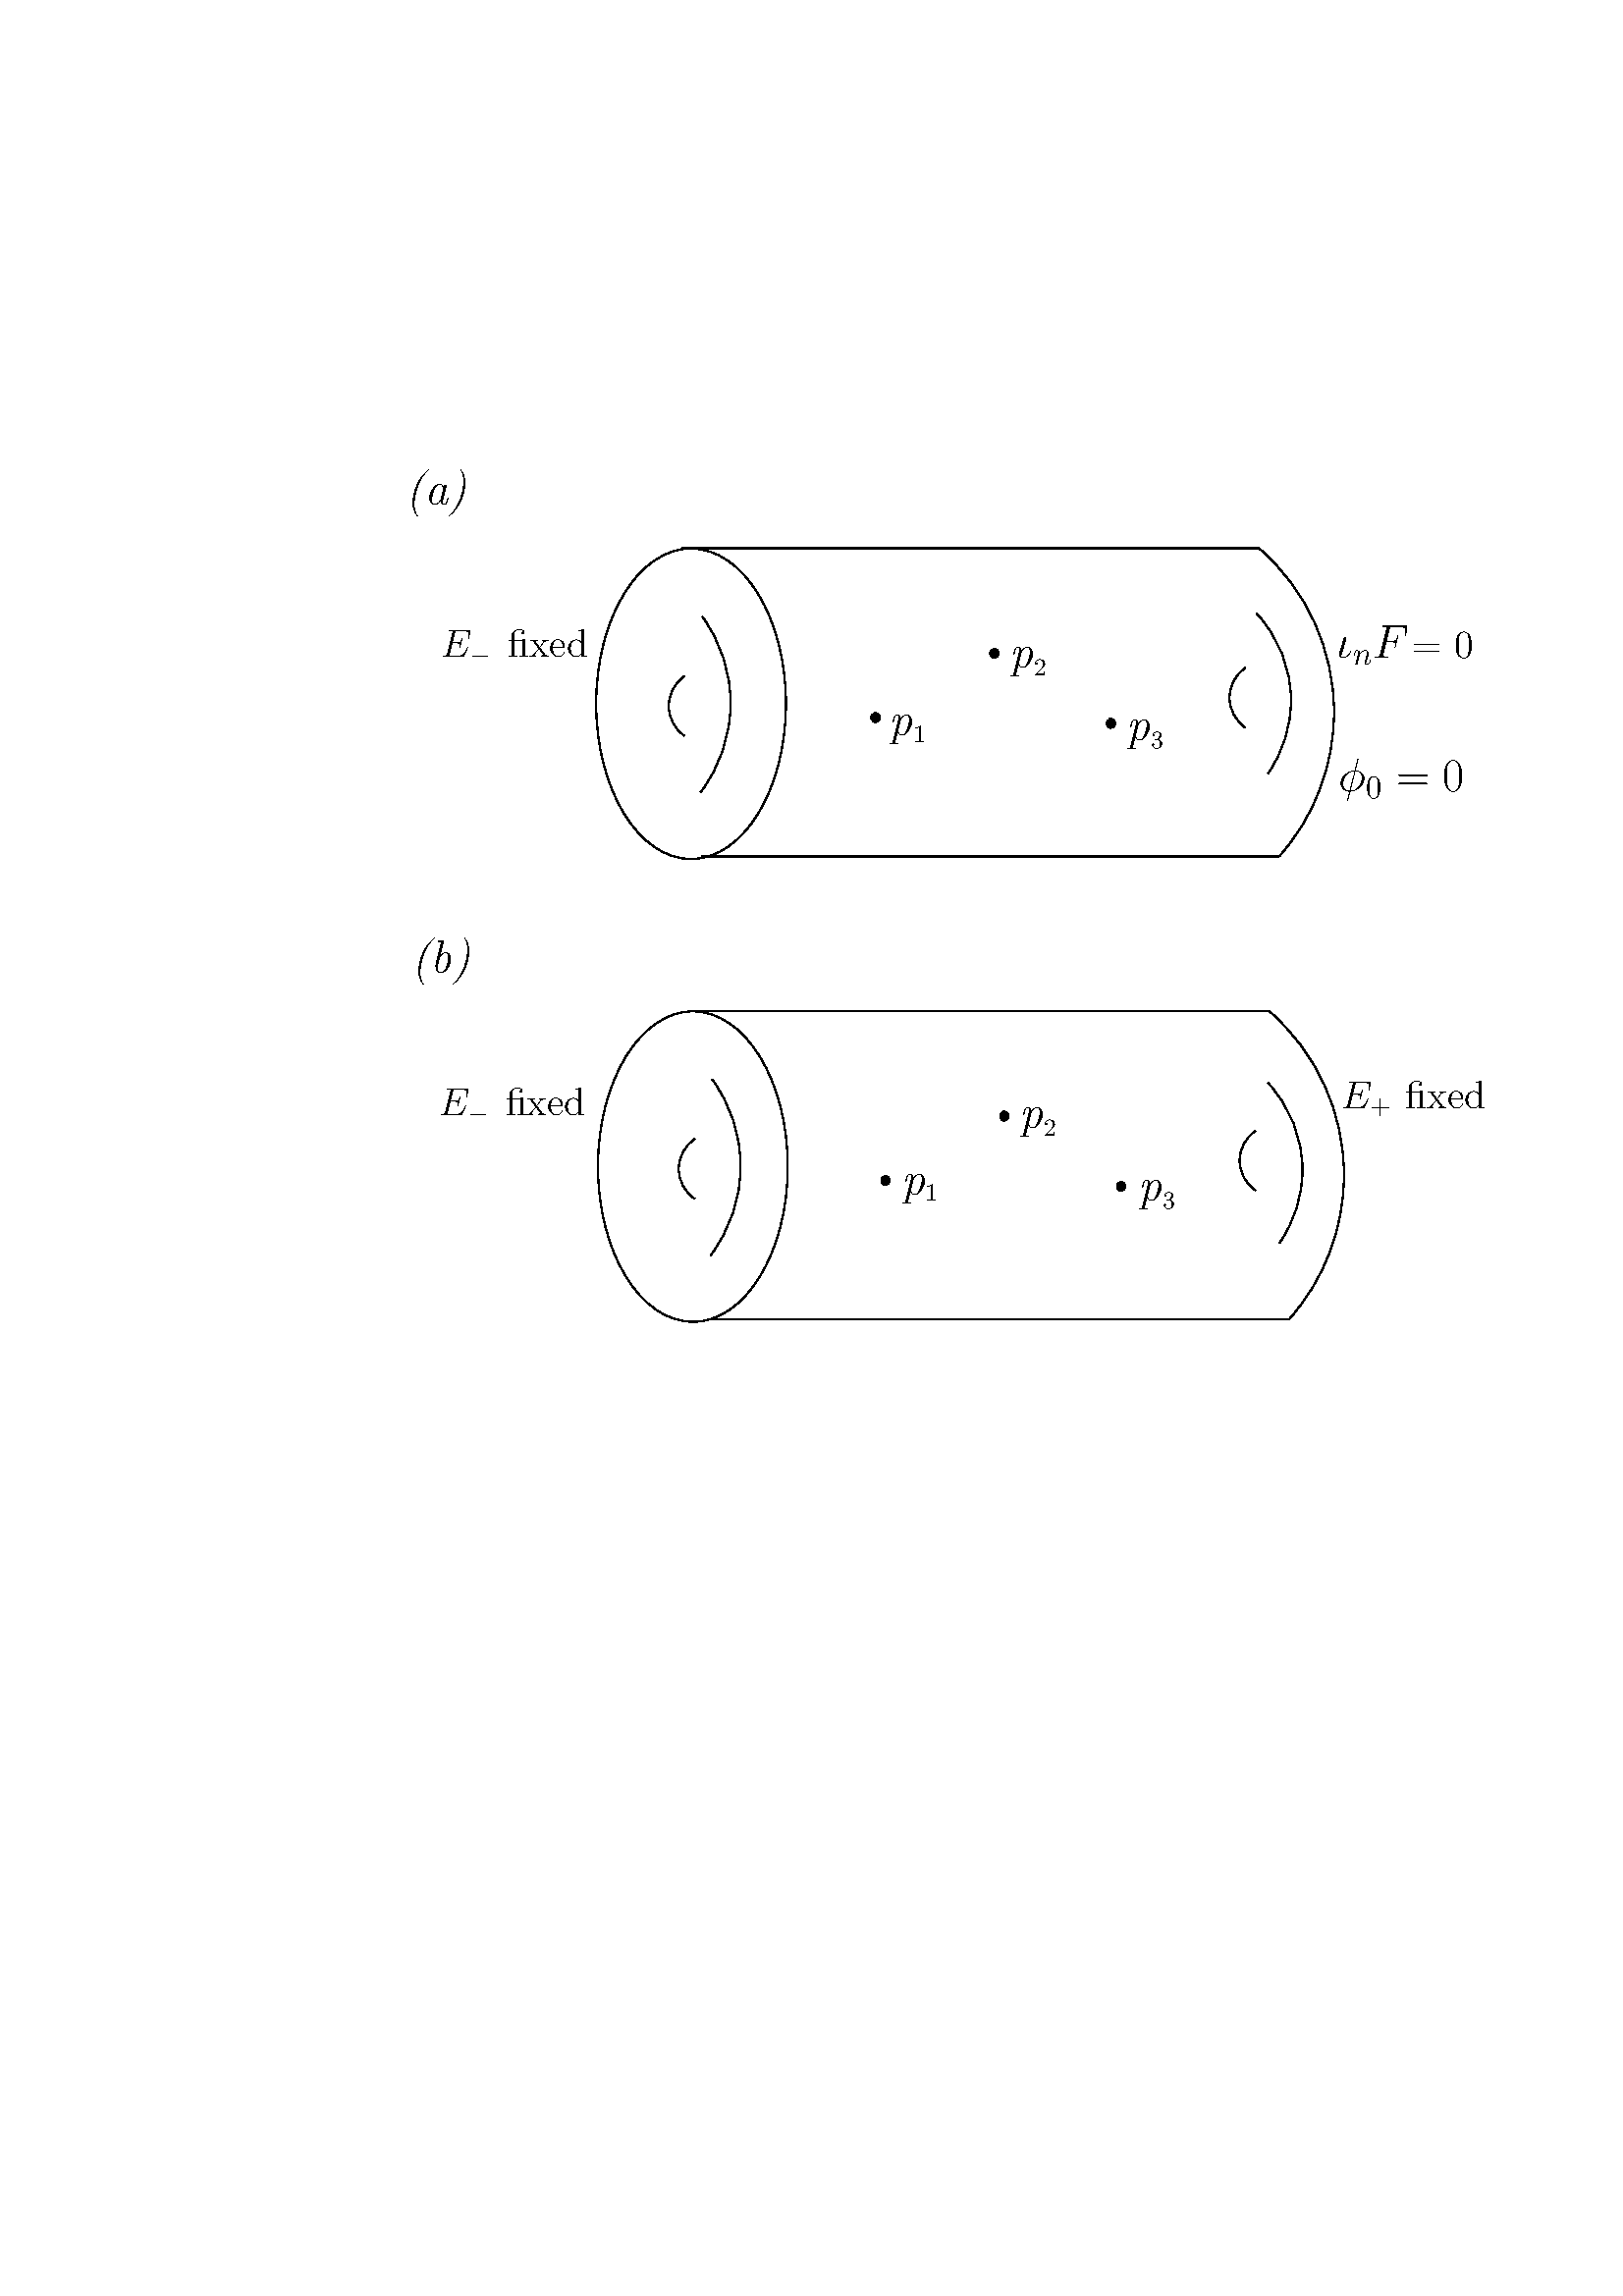
\includegraphics[width=0.75\linewidth]{figures/gla7-4.png}
\caption{(a) 在带有 't Hooft 算子插入的三维流形 $W=I\times C$ 上，左端指定了一个丛 $E_-$，人们希望确定右端可能出现的 Hecke 修正 $E_+$。左端联络 $A_-$ 满足 Dirichlet 边界条件，$\phi_0$ 未加指定；右端则相反。(b) 为描述 Hecke 对应的纤维，需要同时指定 $E_-$ 与 $E_+$，并在两端都让 $\phi_0$ 未加指定。（原文 Fig.~15）}
\label{fig:utampo}
\end{figure}

我们可能考虑两个密切相关的问题。一个自然的问题是描述 't Hooft/Hecke 算子对丛的作用，第二个是描述 Hecke 对应。

对第一个问题（\utampo(a)），我们在 $W$ 的左端指定一个丛 $E_-$，然后问：通过解带奇点的 Bogomolny 方程，另一端能出现什么样的丛 $E_+$。这样我们应当能重新得到 Hecke 修正空间，如第~\ref{sec:theck}~节 所描述。另一个可选的问题（\utampo(b)）是试图描述 Hecke 对应，它参数化具有适当 Hecke 关系的丛配对。我们将描述适合这两个问题中任何一个的边界条件。

为指定丛 $E_-$，我们指定 $C_-$ 上的规范场 $A_-$。我们要指定的是实际的丛 $E_-$，而不是丛的同构类，所以我们指定 $C_-$ 上一个实际的联络 $A_-$。因此我们只模去那些在 $C_-$ 上为平凡的规范变换。对某些目的而言，方便的做法是假定丛 $E_-$ 稳定，此时可以假定联络 $A_-$ 平坦。我们不假定由解 Bogomolny 方程得到的输出丛 $E_+$ 稳定。

\begin{yizhu}[易错点]
按：这里指定的是 $C_-$ 上一个具体的联络 $A_-$，而不是丛的同构类，因此只模去在 $C_-$ 上为平凡的规范变换；若两端都模去规范变换，得到的对象是 ${\rm Bun}_G$ 上的点而不是给定 $E_-$ 的 Hecke 修正空间。$E_-$ 稳定的假定只是为了能取平坦代表，输出丛 $E_+$ 并未假定稳定。
\end{yizhu}

我们希望 $C_-$ 上的边界条件（在模去规范变换后）是椭圆的。Bogomolny 方程中最简单的椭圆边界条件是：要么对 $A$ 施加 Dirichlet 边界条件（即指定其边界值）而不指定 $\phi_0$ 的边界值，要么反过来。若指定了 $A$ 的边界值，则 Bogomolny 方程会确定 $\phi_0$ 在边界处的法向导数；反之亦然。在 $E_-$ 处，由于我们要指定 $A$，就令 $\phi_0$ 不加指定。若 $A_-$ 平坦，则 Bogomolny 方程要求在 $C_-$ 处 $\phi_0$ 的法向导数为零。

另一方面，在 $C_+$ 处，我们希望允许由 $E_-$ 经解 Bogomolny 方程可能出现的一切 Hecke 修正 $E_+$。所以 $C_+$ 上不指定联络 $A$，而是令 $C_+$ 上 $\phi_0=0$。于是 Bogomolny 方程要求 $A$ 在 $E_+$ 处满足协变 Neumann 边界条件；即其曲率 $F(A)$ 与边界的法向量缩并时为零。我们只关心模去规范变换的输出丛 $E_+$，所以允许规范变换在 $C_+$ 上非平凡。这些边界条件总结在 \utampo(a) 中。在第~\ref{sec:kahstr}~节 中，我们将更深入地理解这些边界条件的自然性。

\begin{yizhu}[物理图像]
按：$C_+$ 端令 $\phi_0=0$ 而让 $A$ 自由（协变 Neumann），与 $C_-$ 端的 Dirichlet 条件恰好互补：Bogomolny 方程是椭圆系统，每端只需在「指定 $A$」与「指定 $\phi_0$」之间二选一，就能得到椭圆问题。$C_+$ 端不指定 $A$，正是为了让所有可能的 Hecke 修正都能出现；若把 $A_+$ 也固定，得到的便是 Hecke 对应在配对 $(A_-,A_+)$ 上的纤维（见下文 \utampo(b)）。
\end{yizhu}

\par\medskip{\it Hecke 对应}

我们刚才描述的是在用 Bogomolny 方程研究 Hecke 算子时一般会采用的边界条件。但我们要停下来讨论一下代数几何中另一种标准表述的微分几何类比。（本文余下部分并不需要这些细节。）与上面把 $E_-$ 看作输入、$E_+$ 看作输出不同，人们可以对称地处理两者，办法是描述「Hecke 对应」。在代数几何的通常表述中，令 ${\rm Bun}_G$ 为 $C$ 上所有 $G$-丛构成的「栈」，不要求稳定。型为 $^L\negthinspace w,z$ 的 Hecke 对应（$^L\negthinspace w$ 是权，$z\in C$ 是点）则是一个簇 ${\cal Q}(^L\negthinspace w,z)$，它映到 ${\rm Bun}_G\times {\rm Bun}_G$。${\cal Q}(^L\negthinspace w,z)$ 在 $E_-\times E_+\in {\rm Bun}_G\times {\rm Bun}_G$ 上的纤维，参数化了在 $z$ 处用型 $^L\negthinspace w$ 的 Hecke 变换把 $E_-$ 变到 $E_+$ 的各种方式。


$E_-$ 与 $E_+$ 之间的关系可以更对称地表述，因为 $C_-$ 与 $C_+$ 由一个保向自同构 ${\cal PT}$ 互换：它在 $C$ 上作用平凡，交换 $I$ 的两端，并且反转时间坐标。这样的自同构把 $\phi$ 映到 ${\cal PT}^*(\phi)$，并把权为 $^L\negthinspace w$ 的 't Hooft 算子映到权为 $^L\negthinspace w'$ 的算子，其中 $^L\negthinspace w'$ 是与 $-{}^L\negthinspace w$ Weyl 共轭的支配权。因此，$E_+$ 由 $E_-$ 经 $z$ 处型 $^L\negthinspace w$ 的 Hecke 变换得到，等价地，$E_-$ 由 $E_+$ 经 $z$ 处型 $^L\negthinspace w'$ 的 Hecke 变换得到。

若权 $^L\negthinspace w$ 较小而 $C$ 的亏格较大，则映到 ${\rm Bun}_G\times {\rm Bun}_G$ 的映射 ${\cal Q}({}^L\negthinspace w,z)$ 的纤维一般是空的。另一方面，若 $^L\negthinspace w$ 足够大，则对任何 $C$ 这个映射一般是纤维化。可以把 ${\cal Q}$ 的定义推广到允许若干具有指定位置与权的 Hecke 算子，此时映射 ${\cal Q}\to {\rm Bun}_G\times {\rm Bun}_G$ 的性质取决于 't Hooft 算子的数目与权。

在微分几何中，${\rm Bun}_G$ 对应于所有联络构成的空间 $\EUA$。$\EUA$ 当然是无穷维的，而 ${\rm Bun}_G$ 是无穷维流形的代数几何类比（它包含任意不稳定的丛，形变空间与自同构群的维数都没有界）。Hecke 对应 ${\cal Q}$ 同样是无穷维的，不会来自椭圆边界条件。Hecke 对应的微分几何版本就是直接把 ${\cal Q}$ 定义为 $W=I\times C$ 上带指定奇点的 Bogomolny 方程所有解构成的空间，模去在两端均为平凡的规范变换。把 ${\cal Q}$ 映到 $\EUA\times \EUA$ 的映射，由把解限制到 $W$ 的两端得到。

${\cal Q}$ 是无穷维的，因为我们在定义它时两端都没有指定 $A$ 或 $\phi_0$；这些边界条件不是椭圆的。在微分几何中，更自然的做法是定义 Hecke 对应在一对联络 $A_-\times A_+\subset \EUA\times \EUA$ 上的纤维。这就是在代数几何中研究映射 ${\cal Q}\to {\rm Bun}_G\times {\rm Bun}_G$ 的纤维的规范理论类比。为此，我们在两端分别固定 $A_-$ 与 $A_+$，并模去在两端均为平凡的规范变换（\utampo(b)）。带这些边界条件的 Bogomolny 方程所有解构成的空间，就是 Hecke 对应在配对 $A_-\times A_+$ 上的纤维。定义这个纤维的边界条件是椭圆的，它相当于在 $W$ 的两端都采用在 \utampo(a) 中只加在 $C_-$ 上的边界条件。

Hecke 对应纤维的虚拟复维数可以用指标理论、通过修改下面给出的讨论来计算。它等于 $-(g-1){\rm dim}(G)$ 加上型 $^L\negthinspace w$ 的 Hecke 修正空间的维数 $\Delta$（也在下面计算）。若虚拟维数是负数 $-d$，意味着 ${\cal Q}$ 一般是 $\EUA\times \EUA$ 中余维为 $d$ 的子簇。若它是正整数 $d'$，意味着 ${\cal Q}$ 一般以维数为 $d'$ 的纤维纤维化于 $\EUA\times \EUA$ 之上。

然而，在余下的分析中，我们集中描述给定丛 $E_-$ 的可能 Hecke 修正构成的空间，因此采用 \utampo(a) 的边界条件。在研究更详细的性质之前，我们先看看能从指标理论学到什么。

\par\medskip{\it 指标理论与虚拟维数}

令 ${\EUZ}$ 为带 \utampo(a) 的椭圆边界条件的 Bogomolny 方程解的模空间。由我们在第~\ref{sec:thooftheckeop}~节 对 't Hooft 算子与 Hecke 算子关系的讨论，可以预期 ${\EUZ}$ 是复流形。我们将在第~\ref{sec:kahstr}~节 证明这一点。Bogomolny 方程的线性化给出 \cite{ref107,ref108} 中研究过的椭圆复形：
% 式 (10.1)
\setcounter{equation}{0}
\begin{equation}\label{eq:tifor}
0\to \Omega^0({\rm
ad}(E))\underarrow{~d_1~}\Omega^1({\rm ad}(E))\oplus \Omega^0({\rm
ad}(E))\underarrow{~d_2~}\Omega^2({\rm ad}(E))\to 0 .
\end{equation}
（这里 $\Omega^i({\rm ad}(E))$ 是取值于 ${\rm ad}(E)$ 的 $i$-形式构成的空间。$d_1$ 是把 $\Omega^0({\rm ad}(E))$（规范变换的 Lie 代数）的元素映到 $A$ 与 $\phi$ 的线性化的映射，其像分别取值于 $\Omega^1({\rm ad}(E))$ 与 $\Omega^0({\rm ad}(E))$。$d_2$ 是 Bogomolny 方程的线性化。）${\EUZ}$ 的切空间是这个复形的一阶上同调群，即 $ H^1={\rm ker}(d_2)/{\rm im}(d_1)$。这个椭圆复形的指标称为 ${\EUZ}$ 的虚拟维数；若其他上同调群 $H^0={\rm ker}(d_1)$ 与 $H^2={\rm coker}(d_2)$ 为零，则它与实际维数一致。$H^0$ 由 $\Omega^0({\rm ad}(E))$ 的协变常值截面组成，它们生成未破缺的规范对称性。在我们的边界条件下，$H^0$ 为零，因为我们要求规范变换在 $W$ 的一端为平凡。如我们将看到的，在 \utampo(a) 的边界条件下，虚拟维数非负。既然如此，$H^2$ 在 ${\EUZ}$ 的奇点之外为零，而 ${\EUZ}$ 的光滑部分是一个流形，其维数等于虚拟维数，即该复形的指标。

\begin{yizhu}[易错点]
按：$H^2$ 的消灭是「虚拟维数＝实际维数」的前提，而 $H^0$ 的消灭则来自边界条件：我们要求规范变换在 $W$ 的一端为平凡，等价于不把两端的规范变换都当作冗余。若在两端都模去规范变换，$H^0$ 会非零，指标与模空间维数就不再一致。另外，$H^2$ 只在 ${\EUZ}$ 的奇点处可能不为零，所以光滑部分确实是维数等于指标的流形。
\end{yizhu}

我们首先分析没有任何 't Hooft 算子时的 Bogomolny 方程。为简单起见，假定 $E_-$ 稳定，并由一个 $F=0$ 的平坦联络代表。（总可以形变到这种情形而不改变指标。）在这种情况下，一种标准的论证表明：带上述任何边界条件的 Bogomolny 方程的解都是从 $C$ 拉回的解，因此特别地 $E_+$ 与 $E_-$ 同构。这其实是第~\ref{sec:vanishing}~节 消灭定理的一个特例，但论证非常简单，我们在此单独给出。

若满足 Bogomolny 方程 $F-\star D\phi_0=0$，则 $0=\int_W\Tr\,(F-\star D\phi_0)\wedge \star (F-\star D\phi_0)$。把它展开并分部积分，得到
% 式 (10.2)
\setcounter{equation}{1}
\begin{equation}\label{eq:notty}
-\int_W\Tr\,\left(F\wedge\star F+D\phi_0 \wedge \star
D\phi_0\right)=-2\int_{\partial W}\Tr\,\phi_0 F.
\end{equation}
边界项在 $\partial W$ 上使 $\phi_0$ 或 $F$ 为零的那个分支上消失。在 \utampo(a) 中，一端有 $F=0$，另一端有 $\phi_0=0$，所以边界项在两端都消失。但 \eqref{eq:notty}\ 的左端是半正定的，只有当 $F=D\phi_0=0$ 时才能为零。因此，在 $E_-$ 平坦的假定下，带这些边界条件且没有 't Hooft 算子的任何 Bogomolny 方程解，都是由从 $C$ 拉回的、$\phi_0=0$ 的平坦联络给出。

特别地，$E_+$ 同构于 $E_-$，而 ${\EUZ}$ 是一个点，维数为零。还可以进一步验证，在带 \utampo(a) 边界条件的这种平凡解附近展开时，$H^2$ 为零。所以在这种情况下，${\EUZ}$ 的虚拟维数与实际维数相同，即零。那么，若把 't Hooft 算子包括进来会怎样？与 't Hooft 算子 $T(^L\negthinspace R)$ 相关联的每个奇点，都把模空间的虚拟维数平移一个量，而这个量只依赖于对偶群的表示 $^L\negthinspace R$（不依赖于 't Hooft 算子所插入的三维流形的细节、丛 $E$ 的拓扑，或其他 't Hooft 算子的可能存在）。这由指标理论的一般切除性质 \cite{ref123} 可得，Pauly \cite{ref124} 证明了它。此外，用我们的语言，Pauly 计算了 't Hooft 算子对模空间维数的贡献，情形为 $G=PSU(2)=SO(3)$、$^L\negthinspace G=SU(2)$。答案\footnote{这是 \cite{ref124} 的定理 I，其中 $k$ 对应于我们所称的 $a/2$。该定理对偶数 $a$ 陈述，因为规范群取为 $G=SU(2)$ 而非 $PSU(2)$，但其证明对奇数 $a$ 也成立，事实上对所有 $G$ 都成立，如我们将讨论的。}是：与最高权 $^L\negthinspace w=(a/2,-a/2)$（$a$ 为正整数）的表示相关联的 't Hooft 算子，把 Bogomolny 方程解的模空间 ${\EUZ}$ 的虚拟（复）维数平移 $a$。

奇点把复维数增加 $a$ 这一事实，与我们第~\ref{sec:spaceheck}~节 通过考察 Hecke 修正空间得到的结果一致。在那里我们证明了：对 $U(2)$ 的权 $(a,0)$，等价地对 $SU(2)$ 的权 $(a/2,-a/2)$，Hecke 修正空间的复维数为 $a$。

Pauly 的证明其实可以直接推广到任意紧 Lie 群 $G$。为解释这一点，我们必须回顾 Pauly 证明背后的技巧，它由 Kronheimer \cite{ref110} 引入。基本想法是考虑四维流形\footnote{Kronheimer 实际上考虑了更一般的情形：把 $\Bbb{C}^2$ 换成更一般的带 $U(1)$ 作用的四维超凯勒流形，并得到 $\Bbb{R}^3$ 上具有更一般奇点集的 Bogomolny 方程解的描述。} $\Bbb{C}^2\cong \Bbb{R}^4$ 上在 ${\EUF}=U(1)$ 作用 $(z_1,z_2)\to (\exp(i\theta)z_1,\exp(i\theta)z_2)$ 下不变的瞬子。商 $\Bbb{C}^2/{\EUF}$ 同构于 $\Bbb{R}^3$。${\EUF}$ 的作用并不自由——它在原点 $z_1=z_2=0$ 处有不动点——但尽管如此，商 $\Bbb{C}^2/{\EUF}$ 仍是流形 $\Bbb{R}^3$。从 $(z_1,z_2)\in \Bbb{C}^2$ 到 $\vec x\in \Bbb{R}^3$ 的映射为

\begin{yizhu}[原文疑误]
按：原文此处脚注写「solutions of the Bogomolny solutions on $\Bbb{R}^3$」，其中第二个 solutions 应为 equations，即「$\Bbb{R}^3$ 上 Bogomolny 方程的解」。译文按后一意思译出；这是作者笔误，语法上也无从解释。
\end{yizhu}

\begin{yizhu}[物理图像]
按：Kronheimer 的技巧把四维的 $U(1)$-不变瞬子与三维的 Bogomolny 方程解对应起来：$U(1)$ 在 $\Bbb{C}^2$ 上的作用有不动点，商 $\Bbb{C}^2/U(1)\cong\Bbb{R}^3$，而不动点纤维上的同态 $\rho:U(1)\to G$ 决定 't Hooft 算子的型。Pauly 据此把「奇点对指标的贡献」化为「不动点对等变指标的贡献」，这是等变指标定理的固定点公式（局部化）的标准应用。
\end{yizhu}
% 式 (10.3)
\setcounter{equation}{2}
\begin{equation}\label{eq:nigo}
\vec x=\bar z\vec\sigma z,
\end{equation}
其中 $\vec\sigma$ 是 $2\times 2$ 无迹 Hermite 矩阵（归一化为 $\Tr\,\sigma_i\sigma_j=2\delta_{ij}$，即著名的 Pauli 自旋矩阵）。这提示 $\Bbb{C}^2$ 上 ${\EUF}$-不变的瞬子可能与 $\Bbb{R}^3$ 上有趣的对象有关，但应当预期在 $\Bbb{R}^3$ 的原点（对应于 $\Bbb{C}^2$ 原点处的不动点）会发生某种特别的事情。

$\Bbb{C}^2$ 上 ${\EUF}$-不变瞬子的描述有些微妙。若把 ${\EUF}$ 在 $\Bbb{C}^2$ 上的作用提升为对 $G$-丛 $\hat E\to \Bbb{C}^2$ 的作用，则特别地 ${\EUF}$ 作用在 $\hat E$ 于不动点处的纤维 $\hat E_{0}$ 上。这样的作用由同态 $\rho:{\EUF}\cong U(1)\to G$ 刻画。我们回忆，这样的同态可以解释为 $^L\negthinspace G$ 的一个权，并确定一个 't Hooft 算子 $T(\rho)$。Kronheimer 考虑 $\Bbb{C}^2$ 上给定 $\rho$ 的 ${\EUF}$-不变瞬子，并证明它们等价于 $\Bbb{R}^3$ 上在原点有奇点的 Bogomolny 方程解，而这个奇点用我们的语言表示算子 $T(\rho)$ 的插入。

Pauly 进而证明：型为 $\rho$ 的奇点对 ${\EUZ}$ 虚拟维数的贡献 $\Delta_\rho$，可以由 $\Bbb{C}^2$ 原点处不动点对「计算 $\Bbb{C}^2$ 上瞬子形变的线性算子」的 ${\EUF}$-等变指标的贡献算出。令 ${\rm ad}(\hat E)$ 为由 $\hat E$ 导出的伴随丛，${\rm ad}(\hat E)_0$ 记它在原点的纤维。不动点对指标的贡献涉及 ${\rm ad}(\hat E)_0$ 中的一个迹。（伴随表示出现，是因为瞬子的形变理论涉及一个作用在伴随丛上的椭圆算子。）按照 Pauly 在第 4.2 节中的计算，结果可以描述如下。${\EUF}\cong U(1)$ 在 ${\rm ad}(\hat E)_0$ 上的作用（由 $\rho:{\EUF}\to G$ 与 $G$ 的伴随表示复合得到）分解为特征之和。${\EUF}$ 的任何特征都形如 $\exp(i\theta)\to \exp(im\theta)$，其中 $m$ 是某个整数。由于 $G$ 的伴随表示是实表示，$\rho$ 分解成特征时出现的非零整数成对出现 $c_k,-c_k$，其中可取 $c_k$ 为正。于是 't Hooft 算子 $T(\rho)$ 对 ${\EUZ}$ 虚拟维数的贡献为
% 式 (10.4)
\setcounter{equation}{3}
\begin{equation}\label{eq:xinon}
\Delta_\rho=\sum_kc_k.
\end{equation}
这推广了 $G=PSU(2)$ 的情形，那里只出现一个整数 $c$。Pauly 的分析立刻从 $SU(2)$ 推广到任意 $G$，因为等变指标定理对任意 $G$ 都成立。计算涉及 Lie 代数中的一个迹，由此得到 \eqref{eq:xinon}。

完全不带 't Hooft 算子时，我们的边界条件下的虚拟维数为零。所以带单个 't Hooft 算子 $T(\rho)$ 时，虚拟维数为 $\Delta_\rho$。但带单个 't Hooft 算子时，${\EUZ}$ 恰好就是型为 $\rho$ 的 Hecke 修正空间 ${{\EUY}}(\rho)$。Hecke 修正空间维数的公式 \eqref{eq:xinon}\ 与 $U(N)$（或 $SU(N)$ 或 $PSU(N)$）的结果 \eqref{eq:ydro}\ 一致，并将它推广到任意的紧群 $G$。

由于 't Hooft 算子对指标理论的贡献是局部的，我们可以立刻写出下述一般结果：带任意指定的一组 't Hooft 算子插入时，Bogomolny 方程解的模空间 ${\EUZ}(\rho_1,\dots,\rho_n)$ 的维数。若没有 't Hooft 算子，${\EUZ}$ 的维数为零。每个与同态 $\rho_i:U(1)\to G$ 相关联的 't Hooft 算子 $T(\rho_i)$ 对维数贡献 $\Delta_{\rho_i}$，所以一般地 ${\EUZ}(\rho_1,\dots,\rho_n)$ 的维数为
% 式 (10.5)
\setcounter{equation}{4}
\begin{equation}\label{eq:migoty}
\Delta=\sum_i\Delta_{\rho_i}.
\end{equation}

%% ============================================================
%% 分片 27：原文第 10 节「The Bogomolny Equations And The Space Of Hecke Modifications」（原文 glshort.tex 起于第 8120 行）
%% 由 tools/harvmac2tex.py 从 arXiv 源码（hep-th/0604151v3）自动生成。
%% 只译英文散文；公式、编号、\label、\cite 一律不改。
%% ============================================================

\subsection{单极子冒泡} \label{sec:monbub}

在第~\ref{sec:spaceheck}~节中我们发现，对某个给定类型
$^L\negthinspace w$ 的 Hecke 修正空间
${{\EUY}}(^L\negthinspace w)$，其自然紧化
$\bar {{\EUY}}(^L\negthinspace w)$ 是这样实现的：把若干相伴类型的、
权重更小的 Hecke 修正一并包含进来。

现在我们就能从 Bogomolny 方程的角度看出这一点的缘由。考虑
$\Bbb{R}^3$ 上在原点处具有指定奇异性的一个 Bogomolny 方程解。它
对应于 $\Bbb{C}^2\cong \Bbb{R}^4$ 上的一个等变瞬子。$\Bbb{R}^4$
上的瞬子方程是尺度不变的，因此会出现数学文献中称为「冒泡」
（bubbling）的现象：一个瞬子可以收缩成一点。对于
${\EUF}$-等变瞬子，这个点必然就是 $\Bbb{C}^2$ 的原点。

借助等变瞬子与三维中具有点奇异性的 Bogomolny 方程解之间的
关系 \cite{ref110}（我们把这种解解释为 't Hooft 算子），把上述
图像放到三维来看，就得到一种或可称为「单极子冒泡」（monopole
bubbling）的现象。单极子冒泡（Kronheimer 在未发表的工作中也
独立发现了它，与 \cite{ref110} 有关）之所以相对陌生，是因为它
对于 $\Bbb{R}^3$（或其他完备黎曼流形）上满足通常边界条件的光滑
Bogomolny 方程解并不会发生。恰恰相反，$\Bbb{R}^3$ 上的光滑
单极子具有离散的拓扑分类与特征尺寸，后者涉及 $\Bbb{R}^3$ 上
无穷远处的渐近行为。单极子冒泡只能出现在有 't Hooft 算子存在的
情形；它是一个过程：一个量子化的电荷单位集中到一点（即
't Hooft 算子所在的位置）并随之消失。

下面我们非常简略地利用 $\Bbb{R}^4\cong \Bbb{C}^2$ 上瞬子的
ADHM 构造（ADHM construction）\cite{ref125}，来确定当规范群为
$G=SU(N)$ 时，等变瞬子的冒泡——换言之，单极子冒泡——如何影响
't Hooft 算子的权 $^L\negthinspace w$。（对于其他存在 ADHM
构造的群，即经典群 $SO(N)$ 与 $Sp(N)$，也可以作类似的分析。但
例外群没有 ADHM 构造。）我们将看到，冒泡对权的改变恰好与预期
相符。

我们将沿用 \cite{ref126} 第 3.3 节。为描述 $\Bbb{R}^4$ 上的
$SU(N)$ 瞬子，设 $U$ 是一个二维向量空间（它作为 $\Bbb{R}^4$ 的
旋量丛之一出现），${\EUF}$ 在它上面按矩阵 % 式 (10.6)
\setcounter{equation}{5}
\begin{equation}\label{eq:normalo}
\left(\begin{matrix}e^{i\theta}
& 0 \\ 0 & e^{-i\theta}\\\end{matrix}\right).
\end{equation}
作用。对任何带有 ${\EUF}$ 作用的向量空间 $V$，记 $\chi(V)$ 为
${\EUF}$ 的特征；例如
$\chi(U)=e^{i\theta}+e^{-i\theta}$。为构造瞬子数为 $k$ 的瞬子，
设 ${{\EUH}}$ 是一个 $k$ 维向量空间。再设 $E_\infty$ 是一个
秩为 $N$ 的向量空间（它实际上是瞬子丛在无穷远处的纤维）。瞬子
由如下一个特殊类型的复形
% 式 (10.7)
\setcounter{equation}{6}
\begin{equation}\label{eq:onnos}
0\,\underarrow{~~~~}\,{{\EUH}}\underarrow{\,\,\alpha(z)\,\,}{{\EUH}}\otimes
U\oplus E_\infty\underarrow{\,\,\beta(z)\,\,}
{{\EUH}}\,\underarrow{~~~~}\, 0,
\end{equation}
 其中 $\beta(z)\alpha(z)=0$。就我们此处的有限目的而言，并不需要
这些细节。$\alpha(z)$ 与 $\beta(z)$ 线性依赖于 $\Bbb{C}^2$ 的
复坐标 $z_1,z_2$。对于光滑瞬子，该复形对任何
$z=(z_1,z_2)\in \Bbb{C}^2$ 唯一非零的上同调群是
$H^1(z)={\rm ker}\,\beta(z)/{\rm im}\,\alpha(z)$。由 ADHM 数据
得到的瞬子丛 $E$ 在 $z$ 处的纤维就是 $E_z=H^1(z)$。

为了得到 ${\EUF}$-等变瞬子，我们选取 ${\EUF}$ 在 $E_\infty$ 与
${{\EUH}}$ 上的作用，并要求复形 \eqref{eq:onnos}\ 是
${\EUF}$-等变的。瞬子丛在原点的纤维（记作 $E_0$）特别地就是
相应复形的第一上同调群：
% 式 (10.8)
\setcounter{equation}{7}
\begin{equation}\label{eq:otonos}
0\longrightarrow{{\EUH}}\underarrow{\,\,\alpha(0)\,\,}{{\EUH}}\otimes
U\oplus E_\infty\underarrow{\,\,\beta(0)\,\,}
{{\EUH}}\longrightarrow 0,
\end{equation}
 对一个仅在 $H^1$ 处有非零上同调的等变复形
$0\underarrow{~~~} V_0\underarrow{\,\,\alpha\,\,}
V_1\underarrow{\,\,\beta\,\,} V_2\underarrow{~~~} 0$，其 $H^1$ 的
特征可以写成
$\chi(H^1)=-\chi(V_0)+\chi(V_1)-\chi(V_2)$。特别地
% 式 (10.9)
\setcounter{equation}{8}
\begin{equation}\label{eq:onsno}
\chi(E_0)=\chi(E_\infty)+\chi({{\EUH}})(e^{i\theta}+e^{-i\theta}-2).
\end{equation}

$\chi(E_0)$ 之所以重要，是因为按照 Kronheimer 的构造，当把该
等变瞬子放到三维中解释时，它决定了出现在
$\Bbb{R}^3=\Bbb{C}^2/{\EUF}$ 原点的 't Hooft 算子的权。若
$\chi(E_0)=\sum_{i=1}^N\exp({im_i\theta})$，则这些权为
$^L\negthinspace w=(m_1,m_2,\dots,m_N)$。

当 $\alpha$ 与 $\beta $ 变动到如下情形时，瞬子冒泡就会发生：对
某个分解 ${{\EUH}}={{\EUH}}_1\oplus
{{\EUH}}_2$，复形 \eqref{eq:onnos}\ 分解为两个复形的直和——一个
零复形 % 式 (10.10)
\setcounter{equation}{9}
\begin{equation}\label{eq:teto}
0\,\underarrow{~~~~}\,
{{\EUH}}_1\underarrow{\,\,\,0\,\,\,}{{\EUH}}_1\otimes
U\underarrow{\,\,\,0\,\,\,}{{\EUH}}_1\,\underarrow{~~~~}\, 0
\end{equation}
 与一个复形
% 式 (10.11)
\setcounter{equation}{10}
\begin{equation}\label{eq:ponos}
0\,\underarrow{~~~~}\,{{\EUH}}_2\underarrow{\,\,\alpha(z)\,\,}{{\EUH}}_2\otimes
U\oplus E_\infty\underarrow{\,\,\beta(z)\,\,}
{{\EUH}}_2\,\underarrow{~~~~}\, 0
\end{equation}
 的直和，而后者的上同调只出现在 1 次。所谓「冒泡后的」瞬子丛
$E'$，其瞬子数比原来少了 ${{\EUH}}_1$ 的秩，它以这第二个复形的
第一上同调群为纤维；与 \eqref{eq:onsno}\ 类似，它在原点的纤维
的特征为
$\chi(E'_0)=\chi(E_\infty)+\chi({{\EUH}}_2)(e^{i\theta}+e^{-i\theta}-2)$。
于是
% 式 (10.12)
\setcounter{equation}{11}
\begin{equation}\label{eq:ponzo}
\chi(E'_0)=\chi(E_0)+\chi({{\EUH}}_1)(2-e^{i\theta}-e^{-i\theta}).
\end{equation}

这个公式决定了瞬子冒泡下权的改变。$E_0$ 的权 $m_i$ 与 $E'_0$ 的
权 $m'_i$ 之间满足
% 式 (10.13)
\setcounter{equation}{12}
\begin{equation}\label{eq:yhog}
\sum_{i=1}^N\exp({im'_i\theta})=
\sum_{i=1}^N\exp({im_i\theta})+\chi({{\EUH}}_1)(2-e^{i\theta}-e^{-i\theta}).
\end{equation}

例如，若 ${{\EUH}}_1$ 是一维的、特征为 $\exp(im\theta)$（$m$ 为
某个整数），则 $E_0$ 的权表必须包含 $m+1$ 与 $m-1$（因为
$\chi(E'_0)$ 是系数非负的 Fourier 级数）。\eqref{eq:yhog}\ 表明，
在这次冒泡过程中恰好有两个权发生变化，即
$(m+1,m-1)\to (m,m)$。这对应于我们在第~\ref{sec:spaceheck}~节
讨论过的 't Hooft/Hecke 算子的最简单退化。再举一例：设
${{\EUH}}_1$ 的秩为二，特征为 $\exp({im
\theta})+\exp({im'\theta})$。若 $|m-m'|>1$，我们只是得到上述
类型的一对移动，即把权 $(m+1,m-1,m'+1,m'-1)$ 换成
$(m,m,m',m')$。但若 $m'=m+1$，则 \eqref{eq:yhog}\ 还允许另一种
移动：把权 $(m+2,m-1)$ 换成 $(m+1,m)$。这对应于另一种预期的
't Hooft/Hecke 算子退化。更一般地，若 ${{\EUH}}_1$ 的秩为 $s$、
权为 $m,m+1,\dots,m+s-1$，则 \eqref{eq:yhog}\ 导致一次移动%
\footnote{要实现这次移动，取 ${{\EUH}}={{\EUH}}_1$、
${{\EUH}}_2=0$，并令 $E'$ 为以 $E_\infty$ 为纤维的平凡丛，
即可得到一个具有适当 ADHM 形式的复形。在正文已给出 $E'_0$ 与
${{\EUH}}_1$ 的特征的情况下，满足 \cite{ref126}\ 的式 (3.3.11)
并且给出一个光滑的、瞬子数为 $s$、能通过冒泡退化为 $E'$ 的
瞬子丛 $E$ 的 $\tau_1,\tau_2,\sigma,$ 与 $\pi$ 的
${\EUF}$-不变选取，本质上是唯一的。}：其中 $E_0$ 的权
$(m+s,m-1)$ 被换成 $E'_0$ 的权 $(m+s-1,m)$。对于 $G=SU(N)$，
't Hooft/Hecke 算子的预期退化全都是这种类型移动的复合。对于
一般的 $G$，预期的退化可以由嵌入 $G$ 的各个子群中的 $SU(2)$
瞬子的冒泡生成。

特别要注意：在不要求 ${\EUF}$-不变时，可以认为瞬子是一个一个地
冒泡的；但一旦施加 ${\EUF}$-不变性，情况就不再如此。存在一些
不可约的过程，其中任意多个 ${\EUF}$-不变瞬子同时冒泡。关于
$\Bbb{R}^3$ 上某些 Bogomolny 模空间的详细描述（在适当的极限下
可以从中看到单极子冒泡现象），参见 \cite{ref112,ref113}。

\par\medskip{\it 奇点处的超凯勒结构}

在第~\ref{sec:spaceheck}~节中，我们曾用一个例子指出：给定类型
$^L\negthinspace w$ 的 Hecke 修正的紧化空间
$\bar {{\EUY}}(^L\negthinspace w)$ 虽然不是超凯勒流形，但它的
奇点确实具有超凯勒结构。现在我们可以解释其中的缘由。这些奇点
来自单极子冒泡，而单极子冒泡由 $\Bbb{C}^2=\Bbb{R}^4$ 上
${\EUF}$-等变瞬子的模空间所支配。但 $\Bbb{R}^4$ 上的瞬子模空间
从 $\Bbb{R}^4$ 的超凯勒结构继承了一个超凯勒结构（这一点在 ADHM
构造中是显然的）。由于群 ${\EUF}$ 保持 $\Bbb{R}^4$ 的超凯勒
结构，${\EUF}$-等变瞬子的空间也是超凯勒的（同样，ADHM 构造使
这一点显而易见）。

我们也可以完全在三维的语言中论证——不动用与四维等变瞬子的
联系——单极子冒泡、从而 $\bar {{\EUZ}}({}^L\negthinspace
w_1,\dots,{}^L\negthinspace w_n)$ 的奇点，是由一个超凯勒模空间
支配的。诚然，$\Bbb{R}^3$ 上 Bogomolny 方程解的模空间是超凯勒的
\cite{ref109}。\footnote{这可以用我们稍后为说明 $W=I\times C$ 上
Bogomolny 方程解的模空间具有 Kähler 结构而使用的那类论证来证明。
那些论证在把 $I$ 换成 $\Bbb{R}$ 时同样有效。如果再取
$C=\Bbb{R}^2$，则 $W=\Bbb{R}^3$ 可以有许多种方式写成
$\Bbb{R}^2\times \Bbb{R}$，于是得到的是超凯勒结构，而不只是我们
在第~\ref{sec:kahstr}~节得到的那种 Kähler 结构。} 而
$\bar {{\EUZ}}({}^L\negthinspace w_1,\dots,{}^L\negthinspace
w_n)$ 的空间并不来自 $\Bbb{R}^3$ 上 Bogomolny 方程的解，而是来自
更复杂的三维流形 $W=I \times C$，并带有相当特别的边界条件。所以
$\bar {{\EUZ}}({}^L\negthinspace w_1,\dots,{}^L\negthinspace
w_n)$ 不是超凯勒的。然而，单极子冒泡是一个局部现象。当一个
单极子电荷单位收缩到一点时，其局部结构并不依赖于发生这一过程的
三维流形的细节。因此奇点附近的结构是超凯勒的，就如同身处
$\Bbb{R}^3$ 上一样。

关于这些超凯勒奇点的形变与消解，我们马上还要给出更多细节。

\begin{yizhu}[易错点]
按：本片反复出现的 $^L\negthinspace w$ 中，左上角的 $L$ 表示这是
Langlands 对偶群 ${}^LG$ 的权，而不是某个普通上标；负细空格命令只是
排版用的，不含数学内容。${\EUF}$ 是 macros.tex 里为绕原点的相位旋转
群 $U(1)$ 预留的花体字母宏（harvmac 习惯用 ${\EUS}$、${\EUF}$ 之类表示
「特殊」群），本片中「${\EUF}$-等变」即「$U(1)$-等变」，不要误当作
与 $F$ 有关的对象。另外，$G=SU(N)$ 的对偶群是 $PSU(N)$，所以权
$(m_1,\dots,m_N)$ 只定义到给所有 $m_i$ 同时加同一个常数（差一个中心
特征）；(10.13) 两边作为权表可以整体平移而不改变等式，正文比较
Fourier 系数时用的正是这一自由度。
\end{yizhu}

\begin{yizhu}[含糊点拨]
按：$\chi(H^1)=-\chi(V_0)+\chi(V_1)-\chi(V_2)$ 其实是三项复形的
Euler 特征 $\sum_i(-1)^i\chi(H^i)$；这里只有 $H^1$ 非零，故二者相等。
要点在于右端只依赖复形的项 $V_i$，与微分 $\alpha,\beta$ 无关；因此
即使 $H^1(z)$ 随 $z$ 变动而发生跳跃（这正是冒泡时发生的事），它的
特征仍可由 $E_\infty$ 与 ${{\EUH}}$ 的特征算出。原文「对光滑瞬子只有
$H^1$ 非零」一句省略了 ADHM 数据的非奇异性条件（即实瞬时方程与
稳定性条件，使 $\ker\alpha$ 与 $\mathrm{coker}\,\beta$ 不出现）；缺了它，复形
可以有 $H^0=\ker\alpha$ 或 $H^2$ 非零。
\end{yizhu}

\begin{yizhu}[物理图像]
按：「冒泡」的画面可以这样读：$\Bbb{C}^2=\Bbb{R}^4$ 上的等变瞬子有
一个被 $U(1)$ 对称性保住的尺度模，当它缩到原点时，三维图上看到的
就是「一个量子化的单极子电荷单位在 't Hooft 算子所在点被吞掉」。在
Hecke 修正一侧，这对应权表的一次退化 $(m+1,m-1)\to(m,m)$：两个权并成
一个双重权。换言之，Hecke 修正空间的紧化边界正是由这些冒泡构型铺
出来的；$\bar {{\EUY}}$ 的奇点就是气泡收缩的那一瞬间。
\end{yizhu}

\begin{yizhu}[易错点]
按：(10.12) 看似「凭空多出」一些权，但 $E'_0$ 是真实瞬子丛在原点的
纤维，其特征 $\sum_i\exp(im'_i\theta)$ 的系数必须是非负整数，因此
$\chi(E_0)+\chi({{\EUH}}_1)(2-e^{i\theta}-e^{-i\theta})$ 必须能写成
系数非负的 Fourier 级数；这正是正文用来反推「$E_0$ 必须含有 $m\pm1$」
的依据。注意 $2-e^{i\theta}-e^{-i\theta}$ 的系数 $(1,-1,-1)$ 并非全正，
所以冒泡只会朝「权更集中」的方向发生，不能从虚空中产生权。
\end{yizhu}

\begin{yizhu}[物理图像]
按：奇点为什么是超凯勒的？ADHM 构造把 $\Bbb{R}^4$ 上瞬子模空间写成
超凯勒商（三个 moment map 同时取零再取商），而 ${\EUF}$ 保持
$\Bbb{R}^4$ 的超凯勒结构，故等变瞬子空间继承超凯勒结构；单极子冒泡
由这个空间支配，因此 $\bar {{\EUY}}$ 的奇点局部是超凯勒的。
$\bar {{\EUY}}$ 整体反而不是超凯勒的，因为它来自带边界条件的三维
流形 $W=I\times C$ 上的 Bogomolny 解，而冒泡只是局部现象——原文最后
一段正是这个论证。
\end{yizhu}

%% ============================================================
%% 分片 28：原文第 10 节「The Bogomolny Equations And The Space Of Hecke Modifications」（原文 glshort.tex 起于第 8120 行）
%% 由 tools/harvmac2tex.py 从 arXiv 源码（hep-th/0604151v3）自动生成。
%% 只译英文散文；公式、编号、\label、\cite 一律不改。
%% ============================================================

\subsection{Kähler 结构与 moment map}

\label{sec:kahstr}

我们的下一个目标是证明 ${\EUZ}({}^L\negthinspace
w_1,\dots,{}^L\negthinspace w_n)$ 是一个 Kähler 流形，并且使其复
结构与第~\ref{sec:thooftheckeop}~节所述、相应的 Hecke 修正模空间
一致。这一分析会使许多事情变得更清楚。它将为我们定义 ${\EUZ}$ 时
所采用的边界条件的选择提供新的动机；它将为理解 't Hooft 算子与
Hecke 算子之间的关系提供更精确的框架；它还将使 Hecke 修正空间的
奇点性质变得更加透明。

\begin{figure}[htbp]
\centering
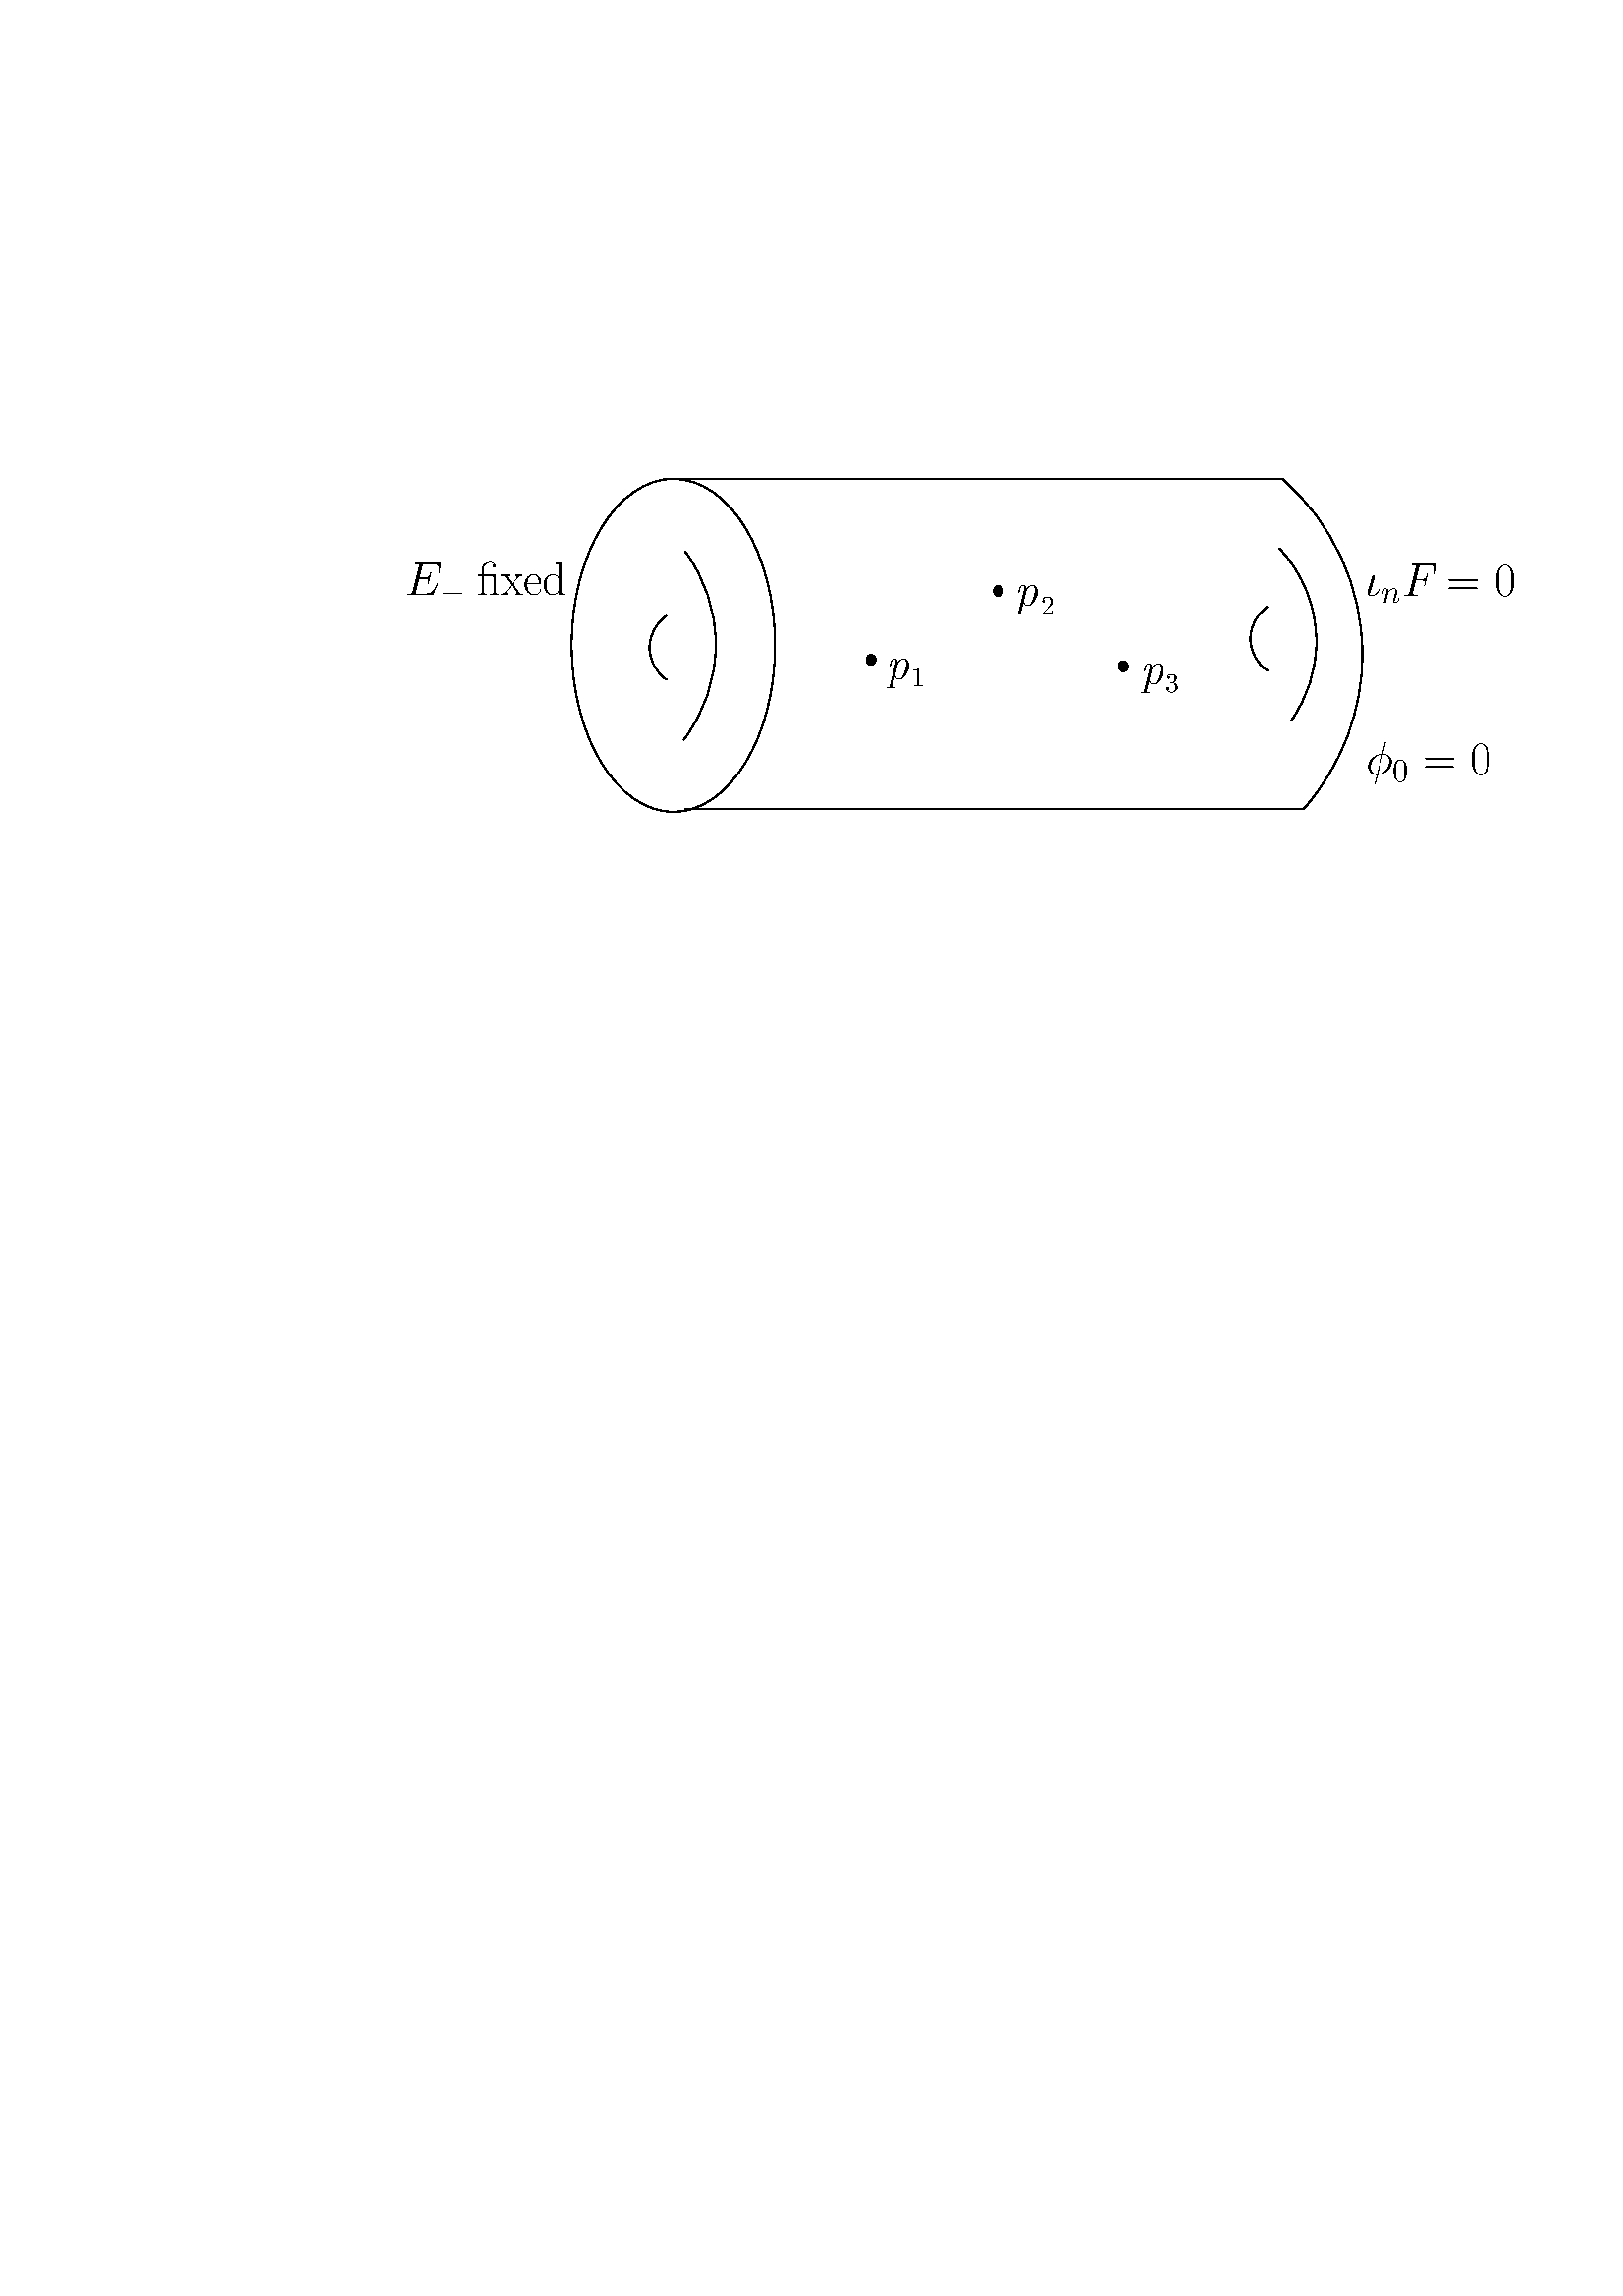
\includegraphics[width=0.75\linewidth]{figures/gla7-5.png}
\caption{在三流形 $W=I\times C$ 上比较 't Hooft 算子与 Hecke 算子。左端给定了联络 $A$ 与丛 $E_-$，并要求规范变换为平凡；右端置 $\phi_0=0$ 并对 $E_+$ 求解。（原文 Fig.~16）}
\label{fig:xutampo}
\end{figure}

正如第~\ref{sec:thooftheckeop}~节引言中那样，我们取三流形
$W=I\times C$ 的度量为 $ds^2=h|dz|^2+dy^2$ 的形式，其中
$z=x^2+ix^3$ 是 $C$ 上的局部复坐标，$y$ 参数化 $I$。我们考虑
Bogomolny 方程 $F=\star D\phi_0$，其中 $F$ 是 $G$-丛 $E$ 上联络
$A$ 的曲率。在 $W$ 的左端，我们指定一个平坦 $G$-丛 $E_-$，并且
只对在边界上等于 1 的规范变换取商；在右端，我们要求
$\phi_0=0$，并对所有规范变换取商。

我们把联络展开为
$A=A_z dz+A_{\bar z}d\bar z+A_ydy=A_2dx^2+A_3
dx^3+A_ydy$。改写 \eqref{eq:noffo}\ 与 \eqref{eq:jungol} 之后，
Bogomolny 方程在这些坐标下可以写成一个复方程 % 式 (10.14)
\setcounter{equation}{13}
\begin{equation}\label{eq:mirot}
\left[D_y-i\phi_0, D_{\bar z}\right]=0
\end{equation}
 与一个实方程 % 式 (10.15)
\setcounter{equation}{14}
\begin{equation}\label{eq:irot}
F_{23}=hD_y\phi_0.
\end{equation}

在域 $(A,\phi_0)$ 构成的空间 ${\EUC}$ 上，我们引入复结构
${\cal I}$，其复坐标为 $A_{\bar z}$ 与 $B=A_y-i\phi_0$。这样
选择的理由是：\eqref{eq:mirot}\ 中的复方程在这个复结构下是全纯
的。此外，我们给 ${\EUC}$ 赋予辛结构 % 式 (10.16)
\setcounter{equation}{15}
\begin{equation}\label{eq:uryt}
\omega=\int_{W}\Tr\Bigl(\delta A_2\wedge
\delta A_3-h\,\delta A_1\wedge \delta\phi_0\Bigr) dx^2\,dx^3\,dy.
\end{equation}

复结构 ${\cal I}$ 与辛结构 $\omega$ 合起来构成一个 Kähler 结构，
其 Kähler 度量为
% 式 (10.17)
\setcounter{equation}{16}
\begin{equation}\label{eq:ryt}
-\int_W\Tr\Bigl( \delta A_2\otimes \delta A_2+\delta
A_3\otimes \delta A_3+h\,\delta A_y\otimes \delta A_y+h\,\delta
\phi_0\otimes \delta \phi_0\Bigr)dx^2\,dx^3\,dy.
\end{equation}

现在我们来求规范群作用的 moment map $\mu$。照例，辛向量场 $v$
的 moment map $\mu(v)$ 由
% 式 (10.18)
\setcounter{equation}{17}
\begin{equation}\label{eq:charby}
d\mu(v)=\iota_v\omega,
\end{equation}
 刻画，其中 $\iota_v$ 是「与 $v$ 缩并」的运算。对于由无穷小
规范变换 $\delta A=-D\epsilon$ 与
$\delta\phi_0 =[\epsilon,\phi_0]$（其中
$\epsilon\in \Omega^0(C,{\rm ad}(E))$）所刻画的向量场，求得
moment map 为 % 式 (10.19)
\setcounter{equation}{18}
\begin{equation}\label{eq:prigo}
\mu(\epsilon)=\int_W\Tr\left(\epsilon(
\,F_{23}-hD_y\phi_0)\right)dx^2\,dx^3\,dy+ \int_{\partial
W}\,\Tr\,(\epsilon\phi_0) \,h\,dx^2\,dx^3.
\end{equation}
 计算与推导式 \eqref{eq:joget} 时类似，只是分部积分时会多出一个
边界项。

当在点 $p_i\in W$ 处有 't Hooft 算子时，我们略微修改这些定义。
要求 $A$ 与 $\phi_0$ 在 $p_i$ 附近具有指定的奇异性。并且约束
$\epsilon$ 在 $p_i$ 附近生成保持所选奇异性不变的规范变换。在这种
情形下，我们的 moment map 公式仍然成立。

我们希望把实 Bogomolny 方程 \eqref{eq:irot}\ 解释为 moment map
取零。事实上，$\mu(\epsilon)$ 为零确实给出 \eqref{eq:irot}，
并附带另一个条件：$\Tr\,\epsilon\phi_0$ 必须在边界上为零。在
$W$ 的任一边界分支 $C_\pm$ 上，有两种简单办法保证
$\Tr\,\epsilon\phi_0=0$。可以令边界上 $\epsilon=0$，也就是只允许
在该边界分支上为平凡的规范变换；也可以令 $\phi_0=0$。为定义模
空间 ${\EUZ}$，我们（\xutampo）在 $C_-$ 上用了其中一种边界条件，
在 $C_+$ 上用了另一种。这样我们就为边界条件找到了新的理由：它们
是最简单的、能把 Bogomolny 方程解释为一个全纯方程加 moment map
取零的条件。

现在我们可以援引辛商与复商之间通常的对应。设 ${\EUC}_0$ 是
${\EUC}$ 中由全纯 Bogomolny 方程 \eqref{eq:mirot}\ 的零点所刻画
的子空间。模空间 ${\EUZ}$ 定义为令 $\mu$ 为零并对 $G$-值规范
变换群 ${\cal G}$ 取商。我们可以把它与
${\EUZ}'={\EUC}_0/{\cal G}_{\Bbb{C}}$ 相比较，后者是 ${\EUC}_0$
对 $G_{\Bbb{C}}$-值规范变换构成的复化群
${\cal G}_{\Bbb{C}}$ 的商。

当然，由于边界条件，${\cal G}$ 是在 $W$ 左端为平凡的规范变换群；
同样，${\cal G}_{\Bbb{C}}$ 是在该端为平凡的
$G_{\Bbb{C}}$-值规范变换群。

通常，在把辛商与相应的复商作比较时，必须担心可能出现的不稳定与
半稳定轨道。然而在本情形中，由于规范变换被限制为在 $W$ 的一端
平凡，这类问题不会出现。${\cal G}_{\Bbb{C}}$ 自由作用且轨道是
闭的，所以所有轨道都是稳定的，从而 ${\EUZ}={\EUZ}'$。

分析 ${\EUZ}'$ 是直截了当的。事实上，我们在
第~\ref{sec:theck}~节中已经基本上做了这件事。对任何远离某个
't Hooft 算子所在位置的 $y\in I$，置
$E_y=E|_{ \{y\}\times C}$。复 Bogomolny 方程表明，只要不越过
't Hooft 算子的位置，$E_y$ 的全纯型就与 $y$ 无关。而且，在没有
't Hooft 算子的区间内，这个全纯型是唯一的
${\cal G}_{\Bbb{C}}$-不变量。在跨过 't Hooft 算子时，$E_y$ 经历
Hecke 修正。所以 ${\EUZ}'$ 就是 $E_-$ 在指定奇异性作用下的
Hecke 修正空间。

这样一来，复商与辛商的比较为理解 't Hooft 算子与 Hecke 算子之间
的关系提供了一个精确的框架——我们在第~\ref{sec:theck}~节中只是
不那么正式地作过这种比较。此外，它还将使我们更好地理解
第~\ref{sec:spaceheck}~节中描述过的 Hecke 修正空间的某些性质。

\par\medskip{\it 改变复结构与辛结构}

我们把 $W=I\times C$ 中插入 't Hooft 算子的点 $p_i$ 记作
$y_i\times z_i$，其中 $y_i\in I$、$z_i\in C$。我们想了解模空间
${\EUZ}$ 对点 $p_i$ 的依赖关系。

引入修正后的联络 $A'=A-i\phi_0 dy$ 会很方便。其想法是：若把
$A'=dz\,A'_z+d\bar z \,A'_{\bar z} +dy\, A'_y$ 展开，
则 $A'{}_y$ 与 $A'{}_{\bar z}$ 在复结构 ${\cal I}$ 下是全纯的，
尽管 $A'_z$ 不是。由于 $A$ 是实的，即取值于 $G$ 的实李代数，
$A'_z$（它等于 $A_z$）是 $A'_{\bar z}$ 的复共轭；当然，$A'_y$
不受任何实性条件约束。要描述群在 $(A,\phi_0)$ 对构成的空间
${\EUC}$（它与修正联络 $A'$ 的空间相同）上的全纯作用，只需描述
$A'_{\bar z}$ 与 $A'_y$ 如何变换。$A'_z$ 的变换则由它是
$A'_{\bar z}$ 的复共轭这一事实确定。

把 $W=I\times C$ 看作 $C$ 上的纤维丛，设 $D_I$ 是 $W$ 的保持该
纤维化的微分同胚群。这样的微分同胚在保持 $z$ 不动的同时把 $y$
映到 $\tilde y(y;z,\bar z)$，其中 $\tilde y$ 在 $W$ 的边界上与
$y$ 一致，且 $\partial \tilde y/\partial y>0$。我们如下定义
$D_I$ 在 ${\EUC}$ 上的作用：直接说 $A'_{\bar z}$ 与 $A'_y$ 按
「拉回」的自然方式变换。

注意，我们不能用拉回来变换 $A'$；对 $\beta\in D_I$，运算
$A'\to \beta^*(A')$ 不会保持 $A'_z$ 与 $A'_{\bar z}$ 互为复共轭
这一事实。我们改而定义
$\beta(A')=\beta^*(A')+dz\,\varepsilon$，其中 $\varepsilon$ 由
保持 $A'_z$ 与 $A'_{\bar z}$ 互为复共轭这一条件确定。

$D_I$ 在 $(A,\phi_0)$ 对构成的空间 ${\EUC}$ 上的这个作用保持复
结构 ${\cal I}$。它也保持复 Bogomolny 方程，因而保持该方程解的
空间 ${\EUC}_0$。这些陈述依赖于 $D_I$ 中微分同胚保持 $z$ 不动
这一事实。因此它们保持由 $\partial/\partial y$ 与
$\partial/\partial \bar z$ 生成的叶状结构，而「沿该叶状结构的叶
平坦」这一断言——正是复 Bogomolny 方程的内容——是不变的。此外，
$D_I$ 把 ${\EUC}$ 的 $G_{\Bbb{C}}$-值规范变换群
${\cal G}_{\Bbb{C}}$ 映到自身。所以由
${\EUZ}={\EUC}_0/{\cal G}_{\Bbb{C}}$ 定义为复流形的 ${\EUZ}$
在 $D_I$ 下不变。

然而，${\EUC}$ 上的辛形式 $\omega$ 肯定不是 $D_I$-不变的，
相应地，${\cal G}$ 作用的 moment map 以及实 Bogomolny 方程也
不再具有不变性。所以，把 ${\EUZ}$ 理解为用辛结构 $\omega$ 对
${\EUC}_0$ 作 ${\cal G}$ 作用的辛商时，它不是 $D_I$-不变的。

结论是：${\EUZ}$ 的复结构是 $D_I$-不变的，但其辛结构不是。

现在考虑位于点 $p_i=y_i\times z_i$ 的 't Hooft 算子。群 $D_I$
可以沿 $y$ 方向上下滑动这些 $p_i$，方式任意，只有一个限制：若
两个 $p_i$ 处于同一个 $z$ 值，则它们在 $y$ 方向上的顺序是
$D_I$-不变的。结论是：沿 $y$ 方向滑动这些 $p_i$（同时不让 $z$
相同的两个点互相越过）会改变 ${\EUZ}$ 的辛结构，但不改变其复
结构。

这件事有一个反向的版本。${\EUC}$ 辛结构的定义只用到 $C$ 的面积
形式，而不用其复结构。因此 moment map $\mu$ 也同样如此。于是，
只给定 $C$ 的面积形式，我们就可以定义辛商
${\EUC}/\negthinspace/{\cal G}=\mu^{-1}(0)/{\cal G}$。这是一个
无穷维辛流形，其辛结构只依赖于 $C$ 的面积形式。一般而言，在辛
流形中，由一族变动的方程所定义的一族辛子流形具有固定的辛结构。
在我们的应用中，变动的这族方程是复 Bogomolny 方程，它们依赖于
$C$ 的复结构。所以当复结构与各点的位置变动时，${\EUZ}$ 的复
结构可以改变，但辛结构不变。

若 't Hooft 算子插入在点 $p_i=y_i\times z_i\in I\times C$，则在
固定 $y_i$ 的前提下改变 $z_i$（并且不改变任一对 $i,j$ 是否有
$z_i=z_j$），等价于改变 $C$ 的复结构的一个特例。所以这样改变
$z_i$ 会改变 ${\EUZ}$ 的复结构，但不改变其辛结构。

\par\medskip{\it 与全纯结果的比较}

我们可以利用这些观察，对第~\ref{sec:spaceheck}~节中描述过的一些
事实获得新的视角。

\begin{figure}[htbp]
\centering
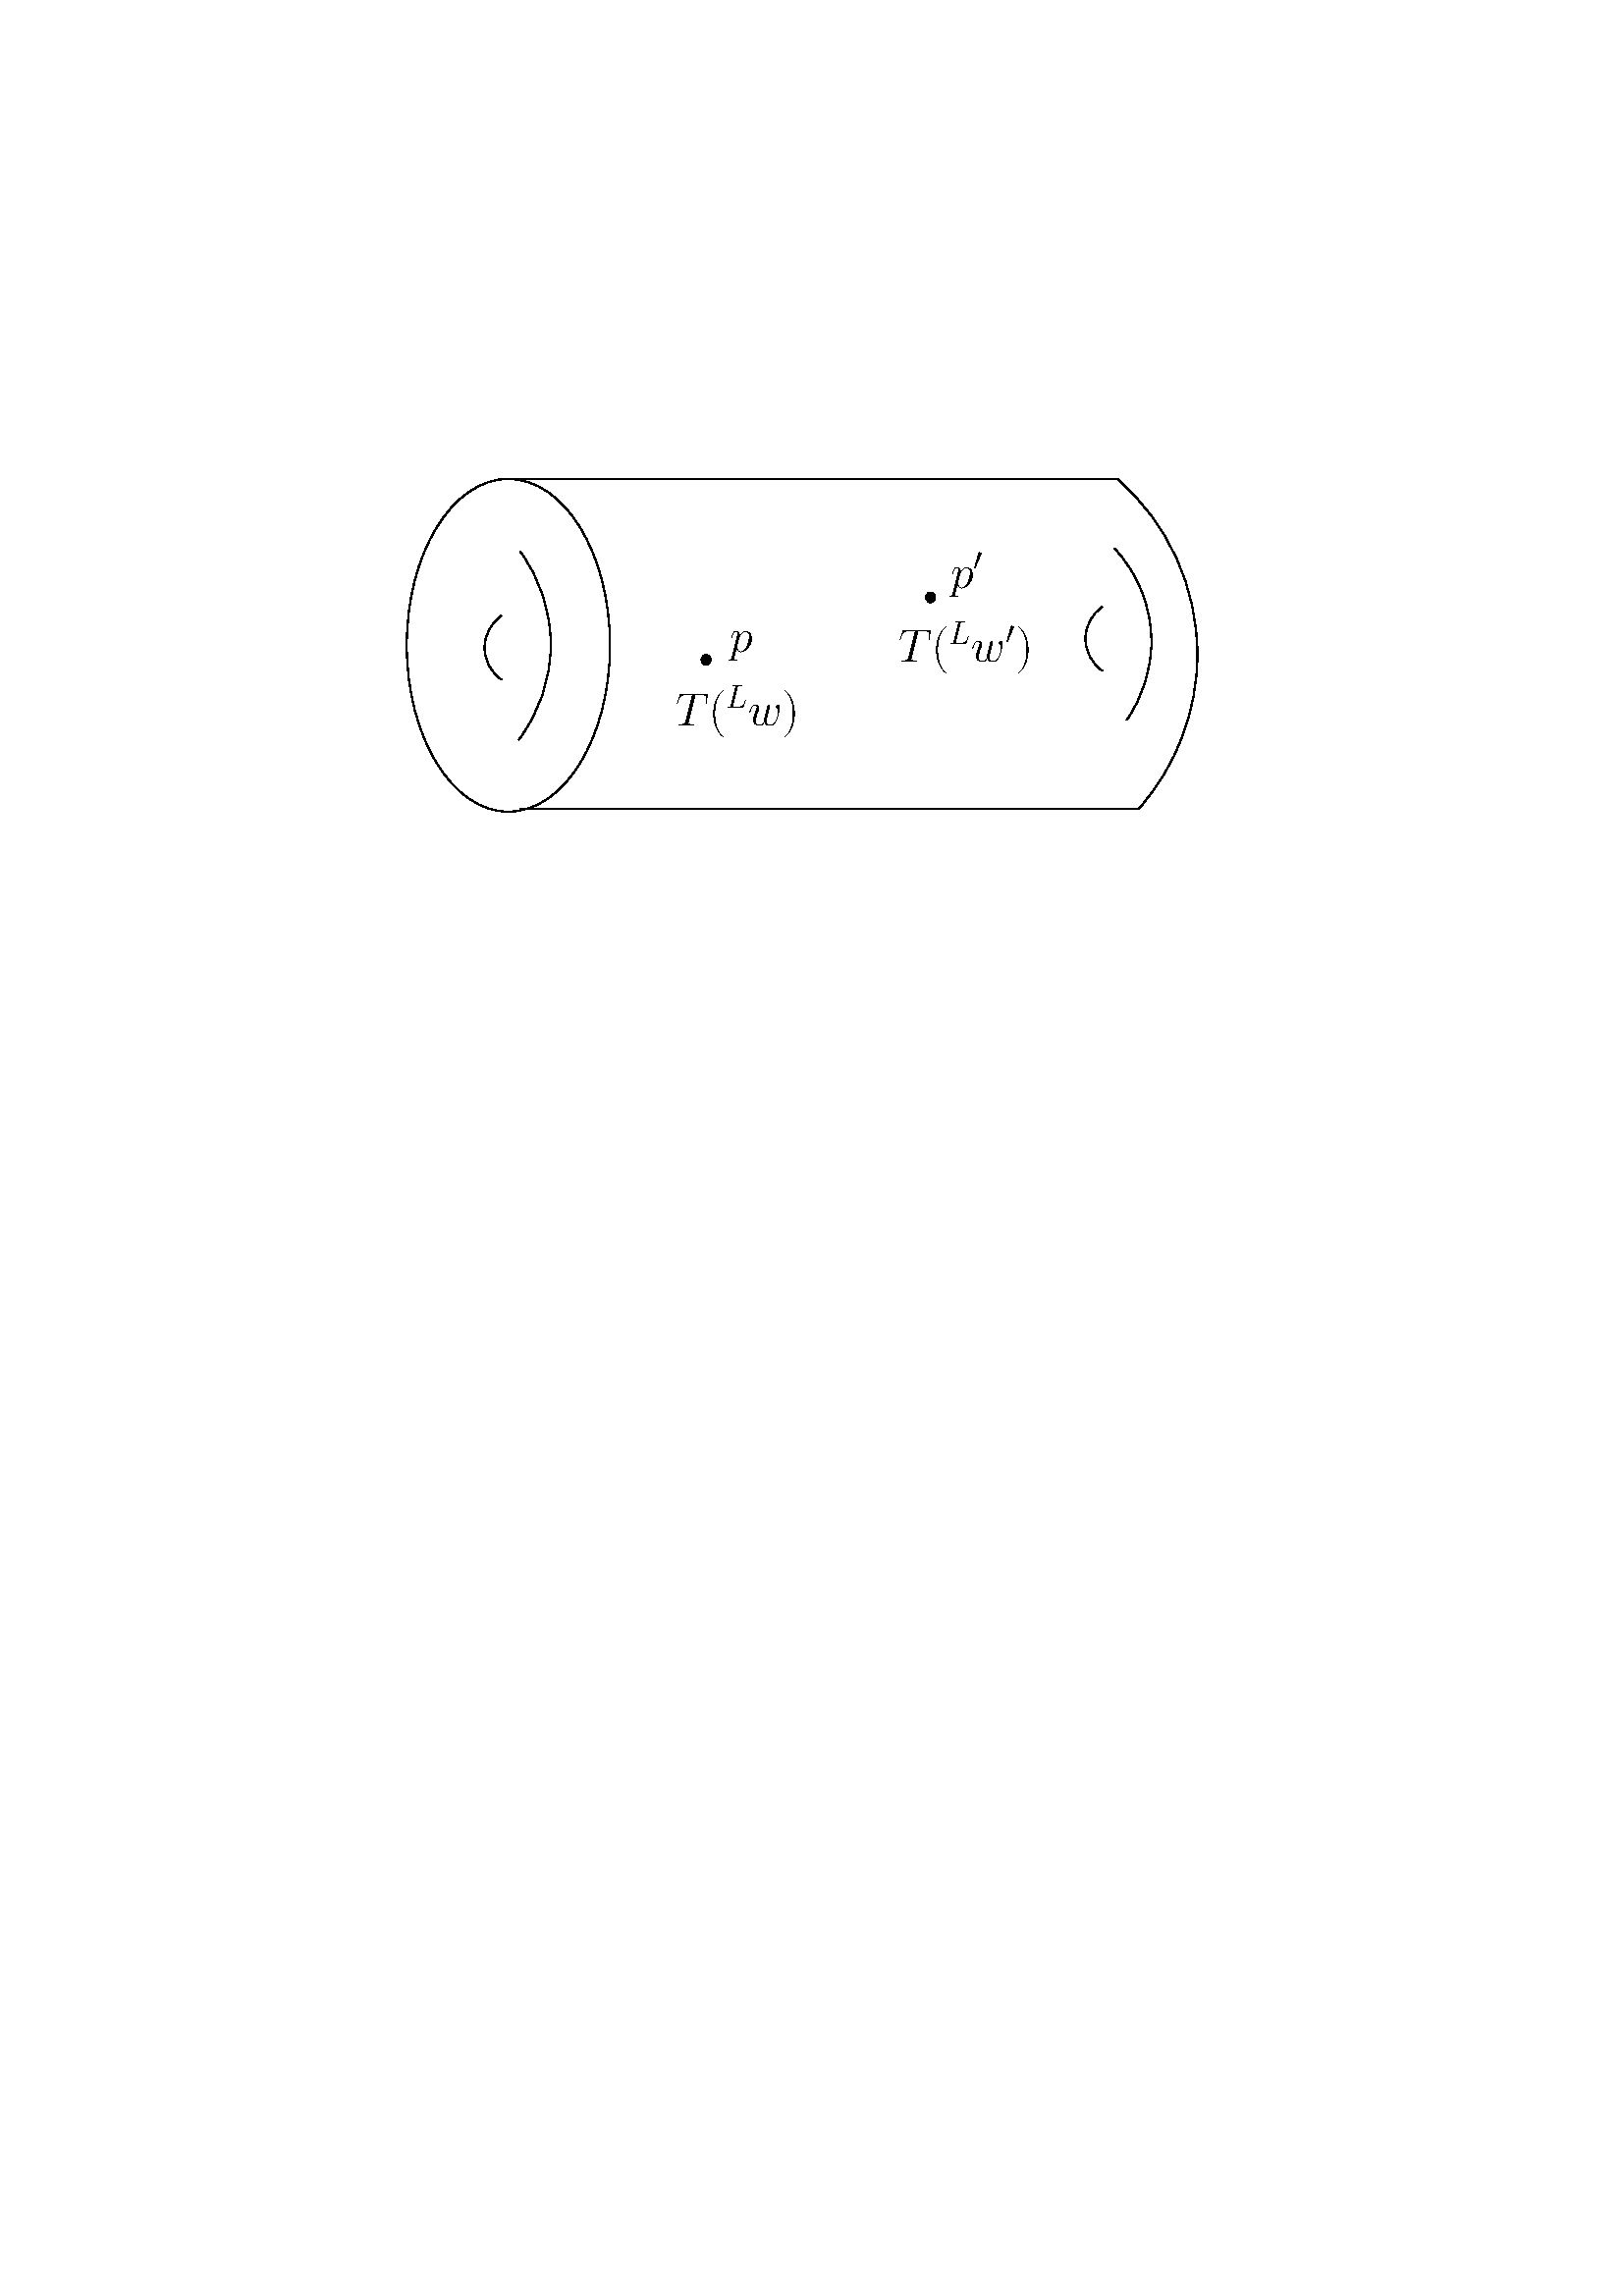
\includegraphics[width=0.75\linewidth]{figures/gla7-6.png}
\caption{在点 $p,p'\in W$ 处插入两个权为 $^L\negthinspace w$ 与 $^L\negthinspace w'$ 的 't Hooft 算子。（原文 Fig.~17）}
\label{fig:xtampo}
\end{figure}

考虑 $W=I\times C$，在其中插入两个指定权的 't Hooft 算子
$T(^L\negthinspace w,p)$ 与 $T(^L\negthinspace w',p')$，插入点为
$p=y\times z$ 与 $p'=y'\times z'$（\xtampo）。我们把相应的紧化
模空间（在 $W$ 左端取某个指定的丛 $E_-$）记作
$\bar{\EUZ}(^L\negthinspace w,p;{}^L\negthinspace w',p')$，或更
简短地记作 $\bar{\EUZ}(p;p')$；同样，把只有一个奇点的类似
Bogomolny 模空间记作 $\bar{\EUZ}(^L\negthinspace w,p)$。

我们可以通过沿 $I$ 方向移动各点（保持到 $C$ 的投影不变）来改变
$\bar\EUZ(p;p')$ 的辛结构；也可以通过沿 $C$ 方向移动各点（保持
到 $I$ 的投影不变）来改变其复结构。

一般来说，$\bar\EUZ(p;p')$ 是奇异的。甚至与单个 't Hooft 算子
（例如 $T(^L\negthinspace w_1)$ 或 $T(^L\negthinspace w_2)$）
相伴的 Hecke 修正模空间也一般是奇异的，正如我们在
第~\ref{sec:spaceheck}~节所讨论的。例外情形对应于
$^L\negthinspace G$ 的极小表示（minuscule representation）。

所以即使 $p\not= p'$，$\bar{\EUZ}(p;p')$ 通常也是奇异的。但当
$p'\to p$ 时它变得更奇异（若原先光滑则产生奇点）。我们把
$p'\to p$ 时的奇异极限记作 $\bar\EUZ{}^*$。我们可以通过沿 $I$
方向移动各点来部分消解 $\bar\EUZ{}^*$ 的奇点，也可以沿 $C$ 方向
移动各点来部分形变这些奇点（\xdtampo）。这种奇点的部分形变与
部分消解在拓扑上是等价的，因为我们可以同时在 $I$ 与 $C$ 两个
方向上移动 $p$ 与 $p'$。

若 $z\not=z'$，则作为复流形 $\bar\EUZ(p;p')$ 是简单乘积
$\bar\EUZ({}^L\negthinspace w,p)\times
\bar\EUZ({}^L\negthinspace w',p')$，它参数化 $C$ 中两个点 $z$ 与
$z'$ 处彼此独立的 Hecke 变换。若 $z=z'$ 且 $y<y'$，则它是
$\bar\EUZ({}^L\negthinspace w,p)$ 上的纤维丛，纤维为
$\bar\EUZ({}^L\negthinspace w',p')$，描述 $E_-$ 在点
$z\in C$ 处依次进行权为 $^L\negthinspace w$ 与
$^L\negthinspace w'$ 的 Hecke 修正。若 $z=z'$ 且 $y'<y$，则
$\bar\EUZ(p;p')$ 仍是纤维丛，只是 $^L\negthinspace w$ 与
$^L\negthinspace w'$ 的角色互换。

\begin{figure}[htbp]
\centering
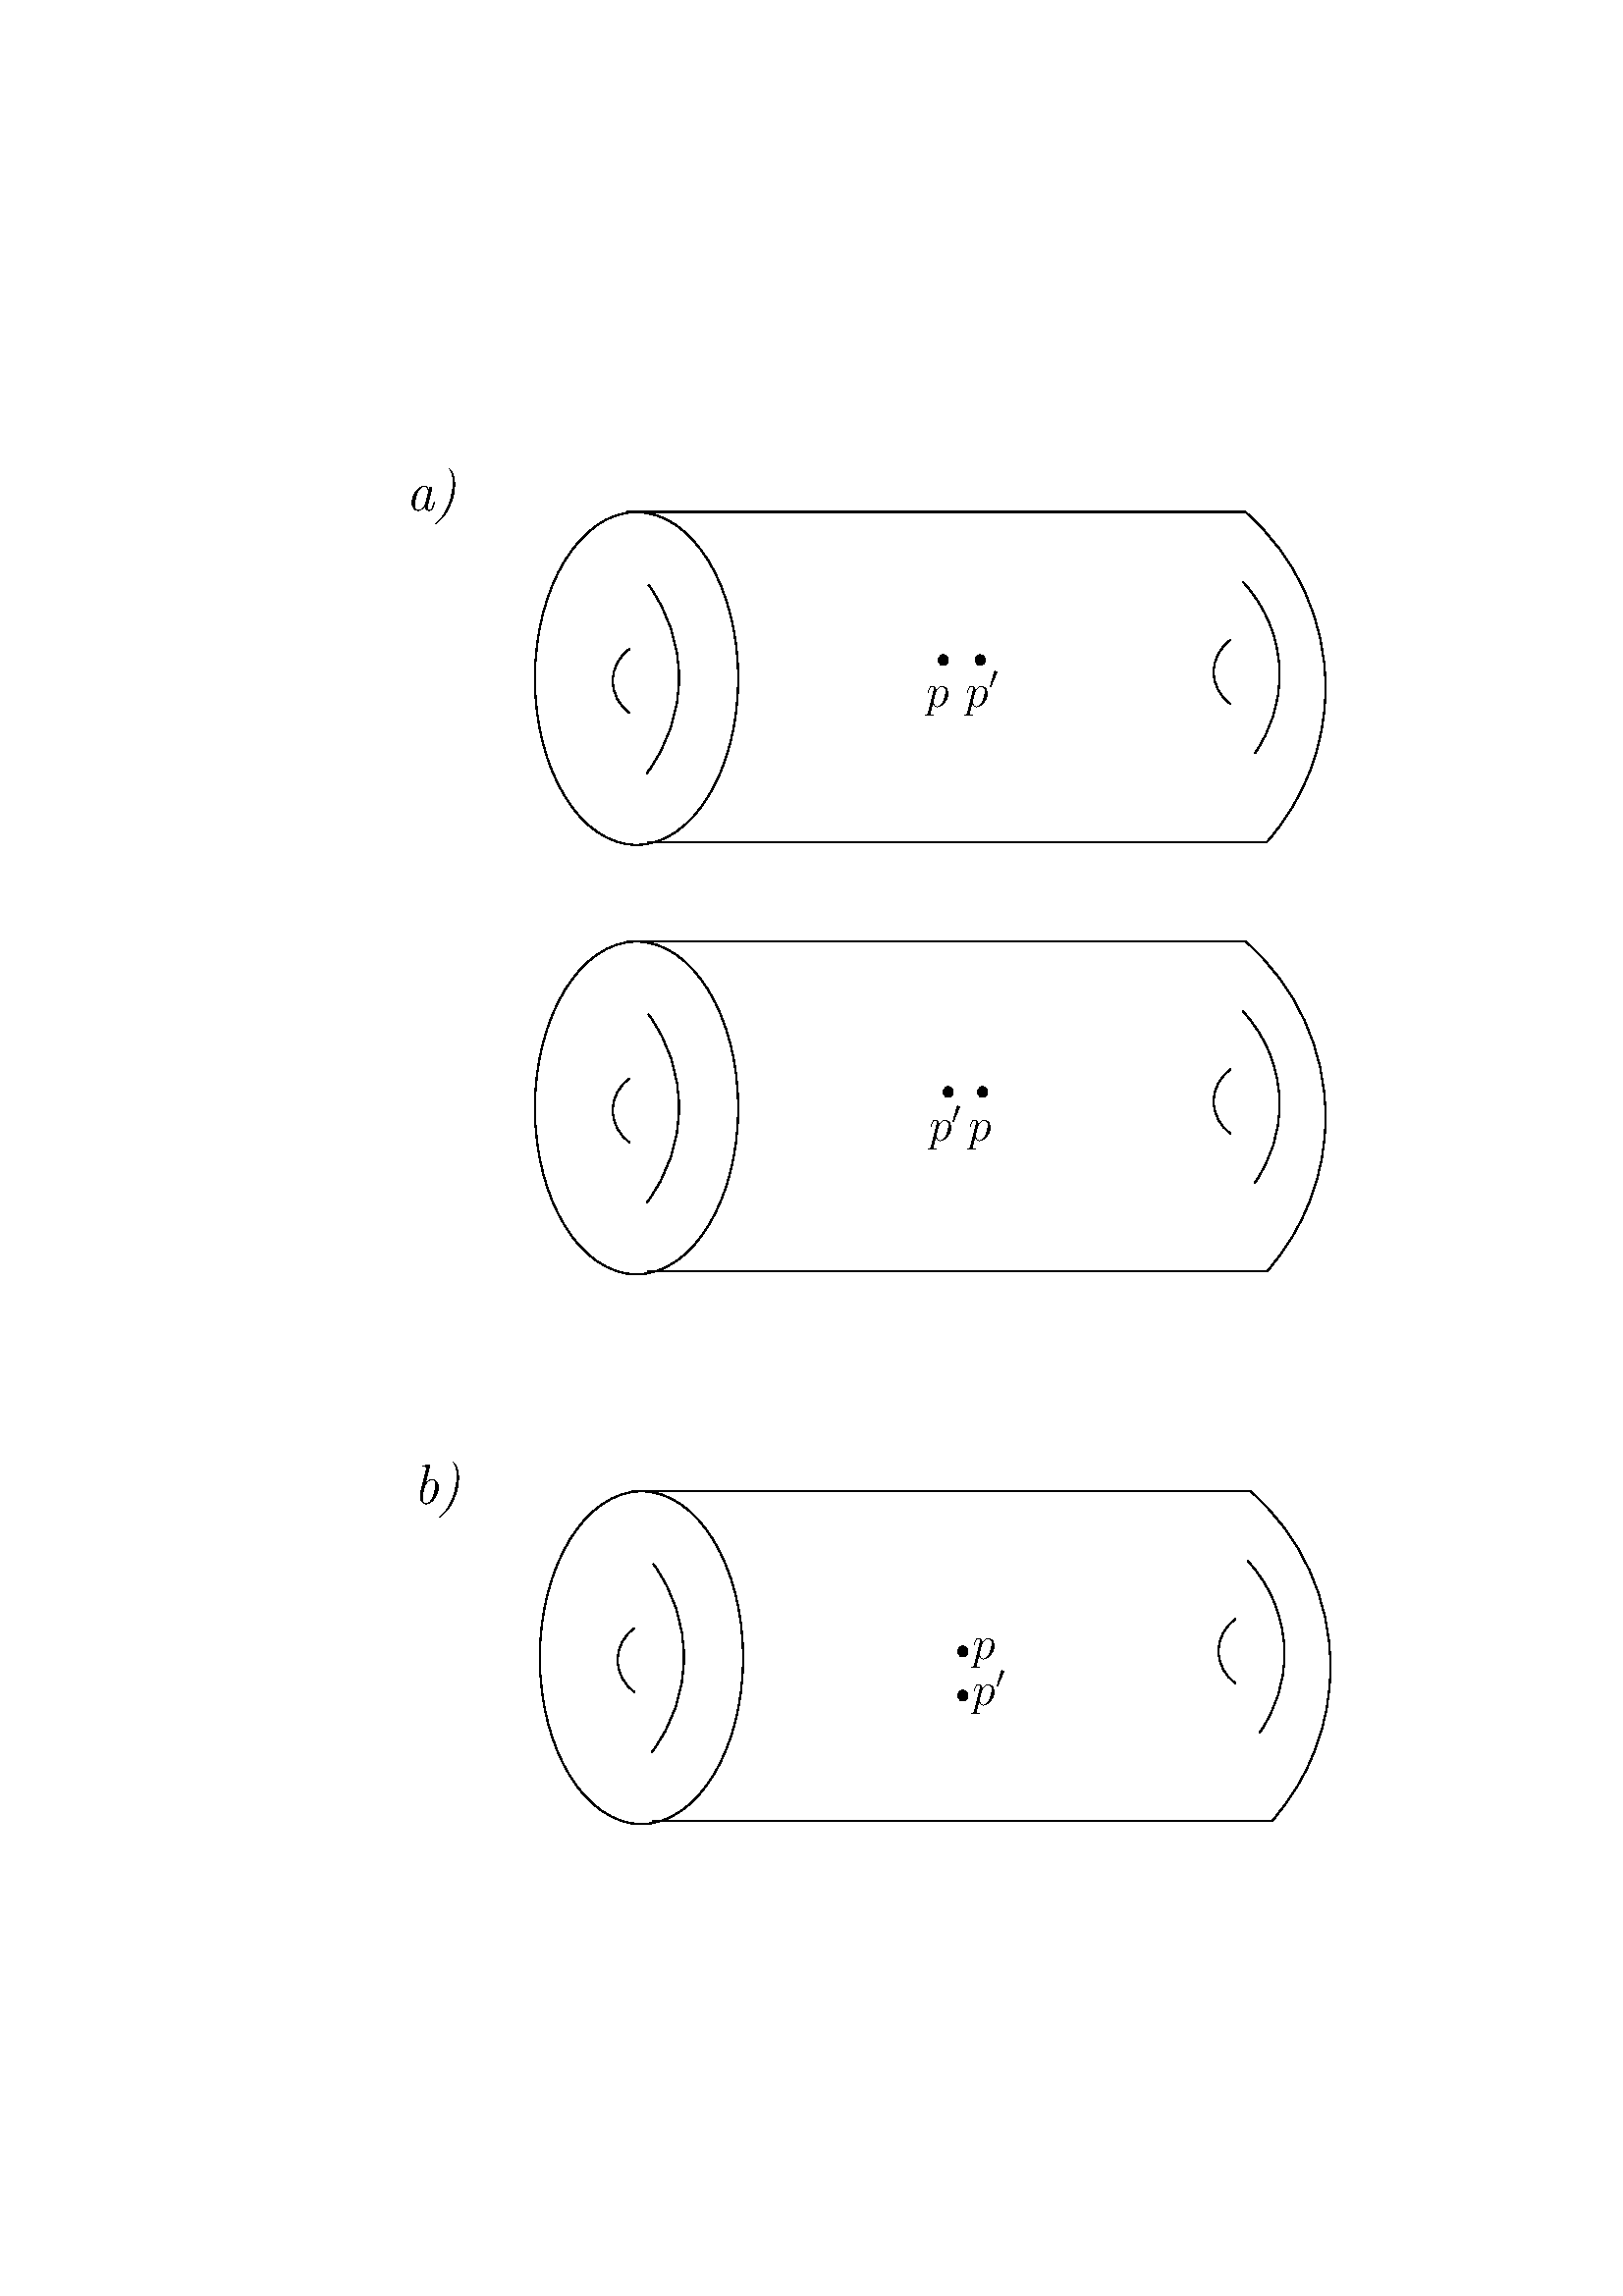
\includegraphics[width=0.75\linewidth]{figures/gla7-7.png}
\caption{（a）奇点的两种部分消解。模空间是一个纤维丛，参数化同一个点 $z\in C$ 处相继的 Hecke 修正。（b）奇点的一种部分形变。模空间是一个乘积，参数化不同点 $z,z'\in C$ 处彼此独立的 Hecke 修正。（原文 Fig.~18）}
\label{fig:xdtampo}
\end{figure}

刚刚描述的、兼有形变与消解的空间 $\bar\EUZ{}^*$ 究竟是什么？
它实际上是 $\bar{\EUZ}(^L\bar w,p')$，即存在单个权为
$^L\bar w={}^L\negthinspace w+{}^L\negthinspace w'$ 的 't Hooft
算子时 Bogomolny 方程解的紧化模空间。

从物理的角度看，这个陈述是算子 $T(^L\negthinspace w,p)$ 与
$T(^L\negthinspace w',p')$ 的算子乘积展开的一部分。我们在
第~\ref{sec:lineop}~节中讨论过这种展开的一些一般性质。那里解释
的简单论证足以说明：乘积 $T(^L\negthinspace w,p)\cdot
T(^L\negthinspace w',p')$ 可以展开为
$\sum_{i\in \EUR}c_i T(^L\negthinspace w_i,p')$，其中
$^L\negthinspace w_i$ 取某个权集 $\EUR$，$c_i$ 为系数。$S$-对偶
预言了该展开的具体形式（它应当与 $^L\negthinspace G$ 的表示环
相吻合），但直接验证这一预言很困难。不过，
第~\ref{sec:lineop}~节中的简单论证确实足以说明：当 $p\to p'$ 时，
展开的形式为
% 式 (10.20)
\setcounter{equation}{19}
\begin{equation}\label{eq:hittor}
T({}^L\negthinspace w,p)\cdot T({}^L\negthinspace
w,p')\to T({}^L\bar w,p')+\sum_{i\in \EUR'} c_i
T({}^L\negthinspace w_i,p'),
\end{equation}
 其中 $^L\bar w={}^L\negthinspace
w+{}^L\negthinspace w'$，而权 $^L\negthinspace
w_i,\,i\in \EUR'$ 是使得 $^L\bar
w-{}^L\negthinspace w_i$ 也为主权的那些主权的权。这意味着
$^L\negthinspace w_i$ 就是我们所说的 $^L\bar w$ 的相伴权重
（associated weight）。

公式 \eqref{eq:xinon} 表明，$\bar\EUZ(^L\bar
w,p')$ 的维数恰好等于
$\bar\EUZ(^L\negthinspace w,p;{}^L\negthinspace w',p')$ 的维数。
这与「前者是后者在 $p\to p'$ 时的极限」这一陈述是一致的。其他
空间 $\bar\EUZ(^L\negthinspace w_i,p')$（$i\in \EUR'$）的维数
严格更小。事实上，在某种意义上，所有空间
$\bar\EUZ(^L\negthinspace w_i,p')$ 都出现在
$\bar\EUZ(^L\negthinspace w,p;{}^L\negthinspace w',p')$ 当
$p\to p'$ 时的极限中。由于这些 $^L\negthinspace w_i$ 是
$^L\bar w_i$ 的相伴权重，按类型 $^L\bar w$ 的 Hecke 修正空间的
自然紧化 $\bar {{\EUY}}(^L\bar w)$ 就包含了所有
$i\in \EUR'$ 的、类型为 $^L\negthinspace w_i$ 的 Hecke 修正空间
$\bar {{\EUY}}(^L\negthinspace w_i)$。用 Bogomolny 模空间的
语言说，这意味着所有空间
$\bar\EUZ(^L\negthinspace w_i,p')$ 都包含在
$\bar\EUZ(^L\bar w,p')$ 的奇异「单极子冒泡」轨迹之中。

这就是为什么确定 't Hooft 算子的算子乘积展开很困难：\eqref{eq:hittor}
中的次领头项全都来自 $\bar\EUZ(^L\bar w,p')$ 的奇点。在
第~\ref{sec:opprod}~节中，我们将解释某些数学结果
\cite{ref97,ref98}，从物理观点看它们等价于确定完整的算子乘积
展开。

不过，我们首先想回顾第~\ref{sec:spaceheck}~节中分析过的一个
例子，它很好地说明了上述论证。取 $G=PSU(2)$、$\LG=SU(2)$、
$^L\negthinspace w={}^L\negthinspace
w'=(1/2,-1/2),$ 以及 $^L\bar w={}^L\negthinspace
w+{}^L\negthinspace w'=(1,-1)$。权 $^L\negthinspace w$ 与
$^L\bar w$ 分别对应于 $\LG=SU(2)$ 的二维表示与伴随表示。正如
我们在第~\ref{sec:spaceheck}~节所知，空间
$\bar {{\EUZ}}(^L\negthinspace w,z)$ 与
$\bar {{\EUZ}}(^L\negthinspace w',z)$ 都是 $\Bbb{CP}^1$ 的拷贝。
空间 $\bar\EUZ{}^*=\bar {{\EUZ}}(^L\bar w,z)$ 是加权射影平面
$\Bbb{WCP}^2(1,1,2)$，具有一个轨形奇点。我们已经发现，这个奇异
空间可以形变为乘积 $\Bbb{CP}^1\times\Bbb{CP}^1$，也可以消解为
一个 Hirzebruch 曲面（它是 $\Bbb{CP}^1$ 上的 $\Bbb{CP}^1$-丛）。
我们还看到，消解与形变是相容的，意思是该 Hirzebruch 曲面可以
形变为 $\Bbb{CP}^1\times\Bbb{CP}^1$。所有这些都与上面的一般论证
相符。（不过在这个特定例子中 $^L\negthinspace w={}^L\negthinspace
w'$，所以两种消解是等价的。）

在这个例子中，把 $^L\bar w$ 写成非零正权之和只有一种方式。一般
地，这样的写法会有若干种，因此沿这些思路对
$\bar {{\EUZ}}(^L\bar w,z)$ 作部分消解与去奇异化就有若干种选择。
对于秩为 $r$ 的单李群 $^L\negthinspace G$，有 $r$ 个基本权
$^L\negthinspace w_\gamma$（$\gamma=1,\dots,r$），使得任何主
权 $^L\bar w$ 都可以用某些非负整数 $t_\gamma$ 唯一地展开为
$^L\bar w=\sum_{\gamma=1}^r t_\gamma {}^L\negthinspace w_\gamma$。
（例如，若 $^L\negthinspace G=SU(r+1)$，则
$^L\negthinspace w_\gamma$ 就是极小表示
$\wedge^\gamma \VV$（$\gamma=1,\dots r$）的最高权。这些表示称为
基本表示。）用 Bogomolny 方程所能做到的、对
$\bar {{\EUY}}(^L\bar w,z)$ 的最大部分消解与去奇异化，就是把它
与一个模空间联系起来：该模空间带有 $t_\gamma$ 个类型为
$^L\negthinspace w_\gamma$ 的 't Hooft 算子插入
（$\gamma=1,\dots,r$）。对 $SU(r+1)$，由于基本表示都是极小的，
这就给出了任意给定权的 Hecke 修正空间的奇点的完全消解或完全
形变。

对其他群，我们能做的最好就是化归为具有基本权的 't Hooft 算子
$T({}^L\negthinspace w_\gamma)$ 的乘积的奇点。这种算子的 Hecke
修正空间带有与单极子冒泡相关的奇点，这些奇点可以局部地用一个
超凯勒流形来模拟，但是对这些奇点没有明显的超凯勒消解。

\begin{yizhu}[易错点]
按：${\cal I}$ 下的复坐标是 $A_{\bar z}$ 与 $B=A_y-i\phi_0$；注意取作
全纯坐标的是 $A_{\bar z}$ 而不是 $A_z$，这与 (10.14) 中 $D_{\bar z}$
所扮演的角色一致。Kähler 度量 (10.17) 带整体负号，是因为 $A$ 与
$\phi_0$ 取值于紧群 $G$ 的李代数，$\Tr$ 在基本表示下负定；只有加上
负号，$\int\Tr(\delta A_i\otimes\delta A_i)$ 才是正定的场空间度量。
另外，(10.16) 中写的是 $\delta A_1$，而 (10.17) 中写的是
$\delta A_y$；由于 $x^1=y$，二者是同一个分量，原文只是记号混用。
\end{yizhu}

\begin{yizhu}[含糊点拨]
按：$\mu(\epsilon)$ 中的边界项
$\int_{\partial W}\Tr(\epsilon\phi_0)h\,dx^2\,dx^3$ 来自分部积分；
正因为有它，$\mu=0$ 才不只给出实 Bogomolny 方程 (10.15)，还要求
边界上 $\Tr\,\epsilon\phi_0=0$。这就是为什么定义 ${\EUZ}$ 时必须
在每个边界分支上二选一：一端令 $\epsilon=0$（只允许平凡的规范
变换），另一端令 $\phi_0=0$。原文只说「有两种简单办法」，其来源
正是这个边界项；而正是这种不对称的选取使得 ${\cal G}_{\Bbb{C}}$
自由作用、轨道闭，从而辛商与复商相等。
\end{yizhu}

\begin{yizhu}[物理图像]
按：$D_I$ 的作用给出「沿 $y$ 移动 = 变辛结构，沿 $z$ 移动 = 变复
结构」的清晰图像。翻成几何语言：把两个 't Hooft 算子在 $C$ 中的
位置分开（$z\ne z'$）得到乘积／形变，把它们重合（$z=z'$）得到
纤维丛／消解。这正对应镜像对称中复结构与辛结构互换的图景：一侧
看到的是复结构的形变，另一侧看到的是辛结构的变分；而
Bogomolny 方程恰好同时提供这两种视角。
\end{yizhu}

\begin{yizhu}[原文疑误]
按：原文「we require $\phi_0=0$ with and divide by all gauge
transformations」中多出一个 with（arXiv v3 源码亦如此），应读作
「require $\phi_0=0$ and divide by all gauge transformations」。
译文按后一读法处理，特此说明。
\end{yizhu}

\begin{yizhu}[原文疑误]
按：本片另有两处原文笔误，均照录：(1) 式 (10.20) 左端第二因子写作
$T({}^L\negthinspace w,p')$，但按上下文（乘积
$T(^Lw,p)\cdot T(^Lw',p')$ 的展开，且 $^L\bar
w={}^Lw+{}^Lw'$）应为 $T({}^L\negthinspace w',p')$；
(2)「Since the $^L\negthinspace w_i$ are associated weights of
$^L\bar w_i$」中的 $^L\bar w_i$ 应为 $^L\bar w$——$\bar w_i$ 在
全文中并无定义，所指的显然是 $^L\bar w$。
\end{yizhu}

\begin{yizhu}[物理图像]
按：'t Hooft 算子的 OPE 有清晰的几何来源：当两个算子互相靠近时，
模空间 $\bar\EUZ(p;p')$ 的极限就是单个算子的模空间
$\bar\EUZ(^L\bar w,p')$，因此领头项是权相加的算符
$T(^L\bar w,p')$；而次领头项来自 $\bar\EUZ(^L\bar w,p')$ 的奇异
轨迹（正是单极子冒泡的所在），故其系数无法由简单论证确定，需要
$S$-对偶／表示环的信息。参见 Frenkel 2009 综述：'t Hooft 函子是
四维 't Hooft 圈算子的二维影子，由「只保持 Higgs 场的那些 Hecke
修正」定义，这与本片边界条件的选取相呼应。
\end{yizhu}

\begin{yizhu}[易错点]
按：极小表示（minuscule）指最高权 $\lambda$ 满足
$\langle\lambda,\alpha^\vee\rangle\le 1$（对一切正根 $\alpha$）
的不可约表示。$SU(r+1)$ 的基本表示 $\wedge^\gamma\VV$ 都是极小的，
故对应的 't Hooft 算子奇点最轻，可由 Bogomolny 方程完全消解。对
一般单李群，基本表示不必极小，于是只能把奇点化归为若干基本权
算子的乘积，而不能再进一步消解——这正是原文最后两段的结论。
\end{yizhu}

%% ============================================================
%% 分片 29：原文第 10 节「The Bogomolny Equations And The Space Of Hecke Modifications」（原文 glshort.tex 起于第 8120 行）
%% 由 tools/harvmac2tex.py 从 arXiv 源码（hep-th/0604151v3）自动生成。
%% 只译英文散文；公式、编号、\label、\cite 一律不改。
%% ============================================================

\subsection{'t Hooft 算子的算子乘积展开}

\label{sec:opprod}

让我们把 $^L\negthinspace G$ 的表示的张量积写成
% 式 (10.21)
\setcounter{equation}{20}
\begin{equation}\label{eq:yurgo}
^L\negthinspace R\otimes {}^L\negthinspace
R'=\bigoplus_{\alpha\in \EUR}\left(N_\alpha \otimes{}^L\negthinspace R_\alpha\right).
\end{equation}

这里 $N_\alpha$ 是向量空间 $N_\alpha={\rm Hom}_G({}^L\neg R\otimes {}^L\neg{R'},{}^L\neg R_\alpha)$，其中 ${\rm Hom}_G$ 指 $G$-不变线性变换构成的空间。集合 $\EUR$ 由那些使 $N_\alpha$ 非零的表示组成。为方便起见，我们还用 $n_\alpha$ 记向量空间 $N_\alpha$ 的维数这个整数。

正如我们在第~\ref{sec:lineop}~节所讨论的，表示的张量积恰好反映在 Wilson 算子的算子乘积展开中。在式~\eqref{eq:tryo} 中，我们用 $c$-数系数 $n_\alpha$ 写出了 Wilson {\it 圈}算子的算子乘积展开。然而，对于静态 Wilson {\it 线}算子——我们把它视为量子化问题的一部分，而不是作用在量子态上的算子——可以写出一个密切相关且更精确的陈述：
% 式 (10.22)
\setcounter{equation}{21}
\begin{equation}\label{eq:docus}
W({}^L\neg R,p)\cdot W({}^L\neg\tilde R,p')\to
\bigoplus_{\alpha\in\EUR}\left(N_\alpha\otimes W({}^L\neg
R_\alpha,p')\right).
\end{equation}

这里我们取规范群为 $^L\neg G$，$p$ 与 $p'$ 是静态 Wilson 算子的位置。\eqref{eq:docus}\ 给出了如下构造的方子：在带有标号为 $^L\neg R$ 与 $^L\neg R'$ 的两个 Wilson 算子时，量子 Hilbert 空间是若干贡献的直和；每一份贡献是在带有一个标号为 $^L\neg R_\alpha$ 的 Wilson 算子时量子化所得量子 Hilbert 空间与向量空间 $N_\alpha$ 的张量积。\eqref{eq:docus}\ 的依据是：在量子理论中，静态 Wilson 算子的效果是引入相应表示中的外源电荷。若有两个静态 Wilson 算子，就有两个外源电荷；把相应表示的张量积分解为不可约表示的直和之后，就得到 \eqref{eq:docus}。

由 $S$-对偶，我们预期 't Hooft 线算子的相应算子乘积展开取同样的形式
% 式 (10.23)
\setcounter{equation}{22}
\begin{equation}\label{eq:zurgo}
T({}^L\negthinspace R,p)\cdot T({}^L\negthinspace
R',p')\to \bigoplus_{\alpha\in \EUR}\left(N_\alpha \otimes T({}^L\negthinspace
R_\alpha,p')\right).
\end{equation}

正如第~\ref{sec:lineop}~节那样，即使不用 $S$-对偶，由于在 $\Psi=0$ 处 't Hooft 算子是唯一的线算子，像 \eqref{eq:zurgo}\ 这样的关系必须以某个表示集合 $\EUR$（它依赖于 $^L\negthinspace R$ 与 $^L\negthinspace R'$）以及某些向量空间 $N_\alpha$ 成立。此外，用简单的论证就足以确定集合 $\EUR$，它依赖于 $^L\negthinspace R$ 与 $^L\negthinspace R'$。所以问题在于描述 $N_\alpha$。

若专门考虑普通的、可以作用在量子态上的 't Hooft 圈算子（相对于会改变量子 Hilbert 空间定义的静态线算子），则算子乘积展开中的系数是普通的 $c$-数 $n_\alpha$，而不是向量空间 $N_\alpha$。实现这种专门化的一种办法是把「时间」方向取成一个圆。这样会对所有量子 Hilbert 空间取迹，向量空间 $N_\alpha$ 便换成了它的整数维数 $n_\alpha$。静态 't Hooft 线算子变成环形的 't Hooft 圈算子（如果改把另一个方向解释为量子化的「时间」方向，它就能作用在量子态上），于是我们得知：'t Hooft 圈算子、乃至拓扑场论中任何圈算子的算子乘积展开系数都是整数。

换一种略有不同的说法，让我们回到 Wilson 算子的情形。闭合 Wilson 圈算子通过和乐（holonomy）的迹来定义。取迹把向量空间换成了它的维数。而开 Wilson 算子（对我们重要的例子是静态 Wilson 线算子）用和乐本身来定义，即把它看作某个向量空间上的算子。在分解这类算子的张量积时，「系数」是向量空间 $N_\alpha$，而非整数 $n_\alpha$。就某些目的而言，这一区别并不重要，可以把 $N_\alpha$ 换成它的维数。

\par\medskip{\it 一些有用的膜}

一旦把场景布置妥当，$N_\alpha$ 的确定便是一门数学理论的推论。这门理论发端于 Lusztig 的工作 \cite{ref98}，它把 $G$ 的不可约表示张量积中的重数与 $^L\neg G$ 上仿射 Schubert 簇的相交上同调复形（intersection cohomology complexes）的卷积联系起来；后经 Ginzburg \cite{ref96} 以及 Mirkovic 与 Vilonen \cite{ref97} 提炼为张量范畴的等价。用物理语言说，这一提炼关乎 't Hooft 算子乘积展开的一种描述：其中「系数」是向量空间 $N_\alpha$（如我们的式~\eqref{eq:zurgo}），而不是更传统的、只考虑闭环算子并把 $N_\alpha$ 换成其整数维数 $n_\alpha$ 的描述（如我们的式~\eqref{eq:tryo}）。我们将先为分析搭好框架，在不借助数学的情况下尽可能用纯物理推理推进，然后再尝试阐明相应的数学理论。

\begin{figure}[htbp]
\centering
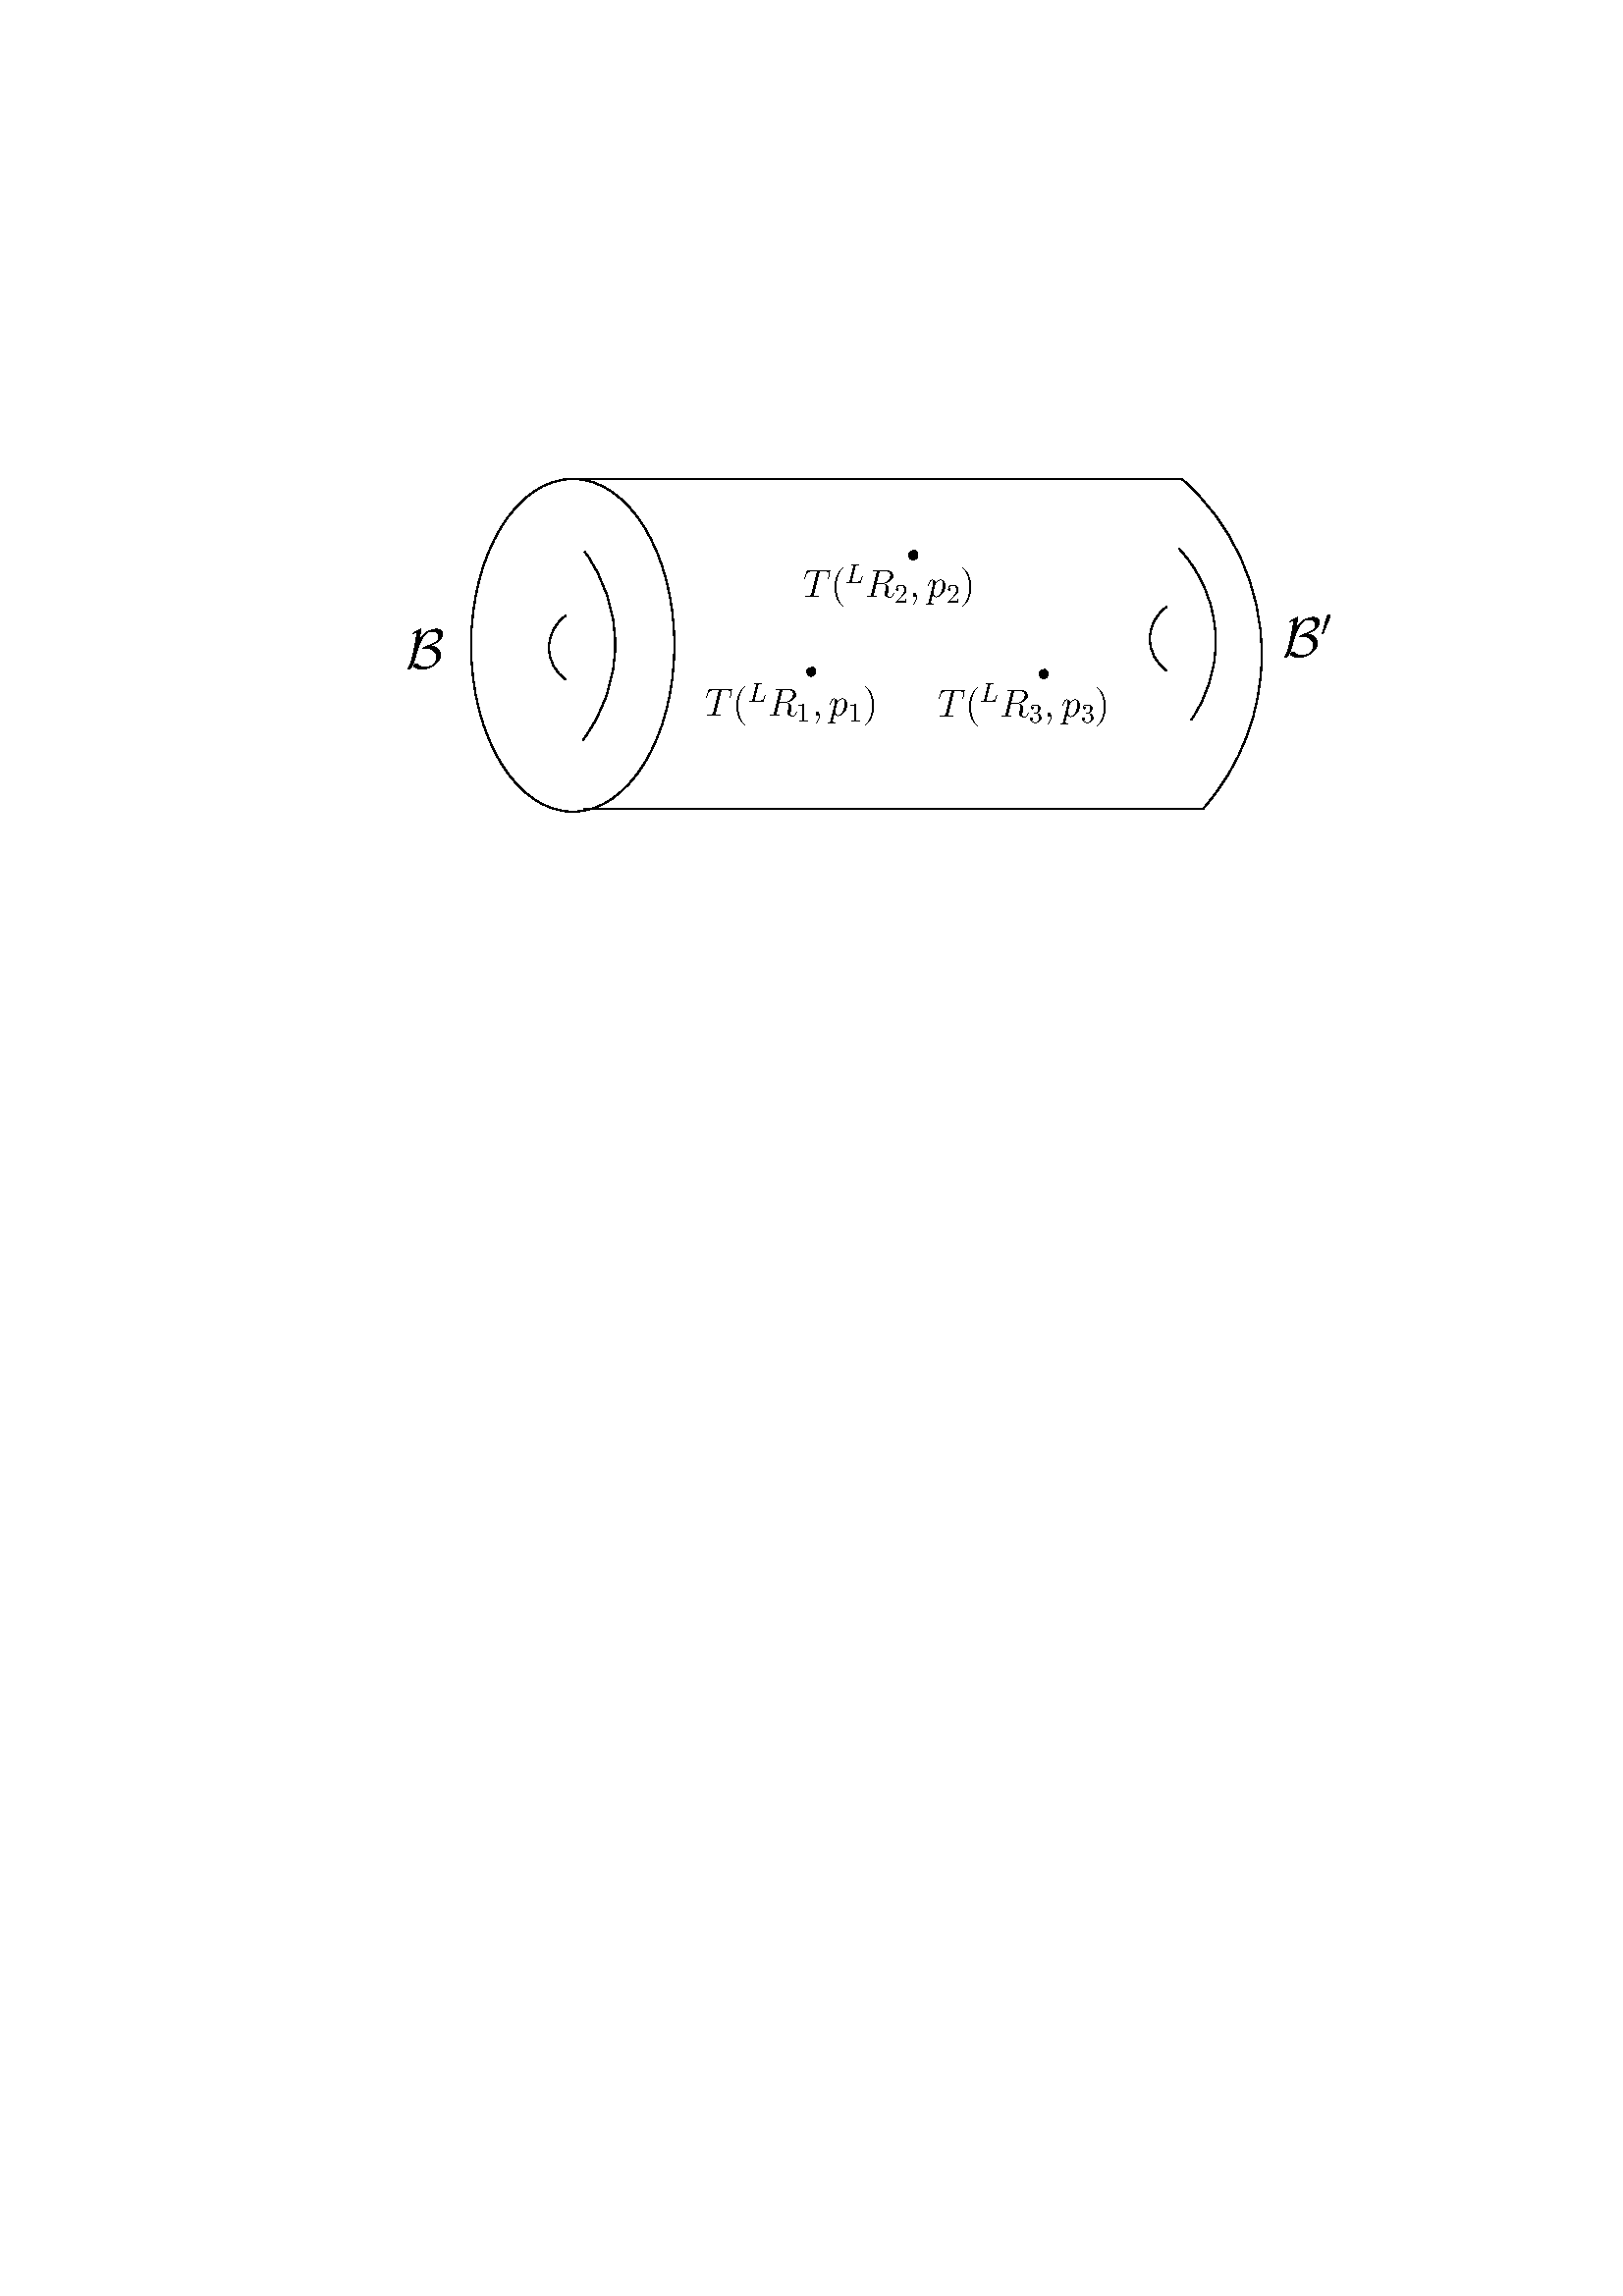
\includegraphics[width=0.75\linewidth]{figures/gla7-8.png}
\caption{Insertion of several 't Hooft operators $T({}^L\negthinspace R_i,p_i)$, with a brane ${\cal B}$ on the left that specifies an ``initial'' bundle $E_-$, and a brane ${\cal B}'$ on the right that sets $\varphi=0$.（原文 Fig.~19）}
\label{fig:xitampo}
\end{figure}

 要确定 $N_\alpha$，只需考虑任意一类方便且足够丰富的、其中静态 't Hooft 算子起作用的计算即可。为此，我们在熟悉的三维流形 $W=I\times C$ 中考虑两个或更多 't Hooft 算子，并在两端选取适当的膜 ${\cal B}$ 与 ${\cal B}'$。我们希望选取那些能使计算简化的膜。

't Hooft 算子保持 $(B,A,A)$ 型超对称，因此最自然的是取 ${\cal B}$ 与 ${\cal B}'$ 为该类型的膜。为此，我们可以取 ${\cal B}$ 与 ${\cal B}'$ 的支撑为 Hitchin 模空间 $\MH$ 中的子簇 $U$ 与 $U'$，它们在复结构 $I$ 中全纯，并且相对于该复结构中为 $(2,0)$ 型的辛形式 $\Omega_I$ 是拉格朗日的。（简言之，$U$ 与 $U'$ 是复结构 $I$ 中的复拉格朗日子流形。）我们给 $U$ 与 $U'$ 配上平凡的 Chan-Paton 线丛。

我们取 $U$ 参数化 Hitchin 对 $(E,\varphi)$，其中要求 $E$ 具有指定的全纯型 $E_-$，而 $\varphi$ 任意。我们要求 $E_-$ 稳定，除此之外 $E_-$ 的选取无关紧要。再取 $U'$ 参数化对 $(E,0)$，其中 $E$ 任意而 $\varphi=0$。

第一点是：$U$ 与 $U'$ 横截相交于唯一一点，对应于 Higgs 丛 $(E_-,0)$。此外，$U$ 与 $U'$ 是复结构 $I$ 中的复辛流形，故 ${\cal B}$ 与 ${\cal B}'$ 是 $(B,A,A)$ 型膜。

最后，我们这样选取 ${\cal B}$ 与 ${\cal B}'$：带这些边界条件、并包含某些 't Hooft 算子时，超对称位形构成的空间恰好就是熟悉的 Bogomolny 方程解的模空间 ${\EUZ}({}^L\negthinspace R_1,p_1;\dots;{}^L\negthinspace R_k,p_k)$。

这个陈述涉及几处微妙之处。首先，超对称位形一般有 $\varphi\not= 0$，必须用第~\ref{sec:thooftheckeop}~节开头描述的扩展 Bogomolny 方程而非普通 Bogomolny 方程来描述。我们甚至还没有分析过扩展 Bogomolny 方程；那将是第~\ref{sec:extbog}~节的主题。到时候我们会看到：若 $\varphi$ 在 $W$ 的一端为零——由于 $U'$ 的选取，这里正是如此——则 $\varphi$ 处处为零，扩展 Bogomolny 方程约化为普通方程。

其次，在描述膜 ${\cal B}$ 与 ${\cal B}'$ 时，我们只描述了以 $\MH$ 为目标的 sigma 模型各场 $(A,\varphi)$ 的边界条件。场 $\phi_0$ 是 Bogomolny 方程的重要组成部分，它出现在规范理论中，却不出现在 sigma 模型中（除奇点处外），因为约化到二维时它是「有质量」的。把第~\ref{sec:zapendix}~节的分析加以推广，可以在规范理论中同时描述膜 ${\cal B}$ 与 ${\cal B}'$ \cite{ref26}，而在那个框架里可以证明：场 $\phi_0$ 的恰当边界条件正是我们所采用的那些。

\par\medskip{\it 物理态的空间}

在 $A$-模型中，没有瞬子修正时（这里不存在瞬子修正，原因见第~\ref{sec:thooftheckeop}~节开头），物理态的空间是时间无关超对称位形空间的上同调。事实上，从物理上理解的 $A$-模型最自然地给出 de Rham 上同调。

换句话说，在膜 ${\cal B}$ 与 ${\cal B}'$ 以及 't Hooft 算子 $T(^L\negthinspace R_i,p_i)$ 之下，物理态的空间就是我们熟悉的、带适当奇点的 Bogomolny 方程解模空间 $\bar\EUZ(^L\negthinspace R_1,p_1;\dots;^L\neg R_k,p_k)$ 的上同调。由于 $\bar\EUZ$ 一般有奇点，这里需要说明所谓的 de Rham 上同调究竟指何种改进。但首先让我们形式地陈述所期待的结果是什么样子。

对每个有限表示集 $^L\negthinspace R_i$（$i=1,\dots,k$），模空间 $\bar\EUZ=\bar\EUZ(^L\negthinspace R_1,p_1;\dots;{}^L\neg R_k,p_k)$ 的上同调给出一个物理态空间 ${\cal H}({}^L\negthinspace R_1,{}^L\negthinspace R_2,\dots,{}^L\negthinspace R_k)=H^*(\bar\EUZ)$。注意，由于底层的四维拓扑场论（TQFT），点 $p_i$ 的选取无关紧要。更确切地说，TQFT 表明：在 $p_i$ 的局部，物理态空间与 $p_i$ 无关（在不同点 $p_i$ 构成的空间上有平坦联络\footnote{移动这些点是改变 $W$ 上度规的特殊情形。度规的改变在 BRST 上同调中是平凡的，这一事实给出该平坦联络。}）。由于三维流形 $W=I\times C$ 中的 $n$ 元组空间是单连通的，也不会有单值性，因此 $p_i$ 无关紧要。所以我们只用表示、而不用点，把物理态空间记为 ${\cal H}({}^L\negthinspace R_1,\dots,{}^L\negthinspace R_k)$。

除开关于奇点的问题，这个论证其实并不需要量子场论。当表示 $^L\negthinspace R_i$ 极小（且 $p_i$ 互异）时，$\bar\EUZ(^L\negthinspace R_1,p_1;\dots;{}^L\neg R_k,p_k)$ 是一族光滑流形。这样一族流形的上同调是局部常值的，正如 TQFT 所预期。在带奇点的一般情形，我们必须确保使用一种能保证这类论证成立的 de Rham 上同调的改进。使这一点成为可能的性质是：$\bar\EUZ(^L\negthinspace R_1,p_1;\dots;{}^L\neg R_k,p_k)$ 虽有奇点，但其奇点结构完全与 $p_i$ 无关。奇点来自单个 Hecke 变换的退化（或单个 't Hooft 算子位置处的单极子冒泡），与其他算子的位置无关。

现在，算子乘积展开说我们可以把 't Hooft 算子的乘积 $T(^L\negthinspace R_1)\cdot T(^L\negthinspace R_2)$ 换成和 $\oplus_{\alpha\in \EUR}C_\alpha\otimes T(^L\negthinspace R_\alpha)$，其中 $\EUR$ 是某个集合，$C_\alpha$ 是某些向量空间。在目前的语境下——针对我们所考虑的膜存在时的物理态空间——这意味着必须有一族同构 % 式 (10.24)
\setcounter{equation}{23}
\begin{equation}\label{eq:mitrox}
{\cal
H}({}^L\negthinspace R_1,{}^L\negthinspace
R_2,\dots,{}^L\negthinspace R_k)\cong\oplus_{\alpha\in
\EUR}\left(C_\alpha \otimes{\cal H}({}^L\negthinspace
R_\alpha,{}^L\negthinspace R_3,\dots,{}^L\negthinspace R_k)\right).
\end{equation}

由于左端只依赖于表示构成的无序集合 $^L\negthinspace R_i$，\eqref{eq:mitrox}\ 中的同构自动与结合律相容，也就是与「反复取算子乘积以进一步减少表示数目」相容。

$S$-对偶表明：集合 $\EUR$ 与向量空间 $C_\alpha$ 应当就是 $^L\negthinspace R$ 的表示张量积中出现的那一组：
% 式 (10.25)
\setcounter{equation}{24}
\begin{equation}\label{eq:omigron}
^L\negthinspace R_1\otimes {}^L\negthinspace
R_2=\oplus_{\alpha\in \EUR}\left(N_\alpha\otimes{} ^L\negthinspace R_\alpha\right).
\end{equation}

其实我们可以更具体一些，只要回忆起\footnote{这些断言与点 $p_i\in W$ 无关，故略去。}：${\cal H}({}^L\negthinspace R_1,^L\negthinspace R_2,\dots,^L\negthinspace R_k)$ 是 $\bar\EUZ({}^L\negthinspace R_1,{}^L\negthinspace R_2,\dots,{}^L\negthinspace R_k)$ 的上同调，而且从拓扑上看 $\bar\EUZ({}^L\negthinspace R_1,{}^L\negthinspace R_2,\dots,{}^L\negthinspace R_k)$ 就是简单乘积 $\prod_{i=1}^k\bar\EUZ({}^L\negthinspace R_i)$。（而 $\bar\EUZ({}^L\negthinspace R_i)$ 等同于 ${}^L\negthinspace R_i$ 型 Hecke 修正的紧化空间 $\bar {{\EUY}}({}^L\negthinspace R_i)$。）乘积的 de Rham 上同调是各因子上同调之积，于是得到 % 式 (10.26)
\setcounter{equation}{25}
\begin{equation}\label{eq:kipro}
{\cal H}({}^L\negthinspace
R_1,{}^L\negthinspace R_2,\dots,{}^L\negthinspace
R_k)=\otimes_{i=1}^k {\cal H}({}^L\negthinspace R_i).
\end{equation}
 这意味着 \eqref{eq:mitrox}\ 必定真正来自一族同构 % 式 (10.27)
\setcounter{equation}{26}
\begin{equation}\label{eq:gitrox}
{\cal H}({}^L\negthinspace R_1)\otimes
{\cal H}({}^L\negthinspace R_2)=\oplus_{\alpha\in \EUR}N_\alpha\otimes
{\cal H}({}^L\negthinspace R_\alpha).
\end{equation}

把 \eqref{eq:omigron}\ 与 \eqref{eq:gitrox} 相比较，我们看到 ${\cal H}({}^L\negthinspace R_i)$ 服从与 $^L\negthinspace R_i$ 相同的张量积代数。这提示存在 ${\cal H}({}^L\negthinspace R_i)$ 与 $^L\negthinspace R_i$ 之间的同构，它给出两个代数之间的自同构。事实上，可以证明 \cite{ref127}：对于有限维向量空间族 $^L\negthinspace R_i$ 与 ${\cal H}(^L\negthinspace R_i)$ 来说，这是它们具有相同张量积代数的唯一途径。${\cal H}({}^L\negthinspace R_i)$ 与 $^L\negthinspace R_i$ 之间的同构在相差 $^L\negthinspace G$ 中元素的共轭意义下唯一。

\par\medskip{\it 按鬼数分次}

由于 $^L\negthinspace G$ 当然以一种与张量积相容的方式作用在 $^L\negthinspace R_i$ 上，这意味着 $^L\negthinspace G$ 也相应地作用在 ${\cal H}({}^L\negthinspace R_i)$ 上（在相差共轭意义下定义）。从物理观点看，这意味着什么是神秘的，因为在 $\Psi=0$ 处 $^L\negthinspace G$ 并不是规范群为 $G$ 的整个 $A$-模型的对称性，而只是我们为分析算子乘积展开所考察的那一小块的对称性。（如果能理解构造中所用膜 ${\cal B}$ 与 ${\cal B}'$ 的 $S$-对偶，事情也许会变得更清楚。）然而，整个 $A$-模型确实有一个相关的对称性。

这就是「鬼数」对称性 ${\EUK}$，它在 ${\EUN}=4$ 超对称杨–米尔斯理论的拓扑扭化中的起源已在第~\ref{sec:twisting}~节解释过。在 $A$-模型中，鬼数粗略地说就是上同调类的次数或维数。\footnote{对 Kähler 目标，Hodge 分解 $H^d(X)=\oplus_{p+q=d}\,H^{p,q}(X)$ 一般会给出 $A$-模型的进一步精细化。然而这与我们目前的讨论无关，因为空间 $\bar \EUZ({}^L\negthinspace R_1,\dots,{}^L\neg R_k)$ 的上同调全为 $(p,p)$ 型。}不过，有一处关键的微妙之处。对复维数为 $n$ 的复流形 $X$，微分形式的次数通常理解为从 $0$ 取到 $2n$。但 $A$-模型的物理态空间有一个费米子共轭对称性\footnote{这里所说的对称性是二维 CPT 对称性。它是具有 $(2,2)$ 超对称、目标为 $X$ 的物理超对称 sigma 模型的精确对称性。在非平坦 Riemann 面 $\Sigma$ 上，这一对称性会被定义 $A$-模型的拓扑扭化破坏。但物理态空间是在平坦流形 $\Bbb{R}\times S^1$ 上量子化 sigma 模型得到的，不受该扭化影响。}，它把维数为 $d$ 的类与维数为 $2n-d$ 的类互换，并把 ${\EUK}\to -{\EUK}$。与次数为 $d$ 的上同调类相应的态，其鬼数实际上是\footnote{为完整起见，我们指出：若 $X$ 是 Calabi-Yau 流形，则 $A$-模型中从态到算子的映射涉及一个谱流，它给 ${\EUK}$ 加上 $\dim_{\Bbb{C}}(X)$。因此若 $\psi$ 是 $X$ 的 $d$ 维上同调中的一个类，则对应于 $\psi$ 的 $A$-模型态满足 ${\EUK}=d-{\rm dim}_{\Bbb{C}}(X)$，而相应的算子 ${\EUO}_\psi$ 满足 ${\EUK}=d$。然而空间 $\bar \EUZ({}^L\negthinspace R_1,\dots,{}^L\neg R_k)$ 并非 Calabi-Yau，更重要的是，我们关于膜与 't Hooft 算子的讨论针对的是物理态，而非相应的算子。} % 式 (10.28)
\setcounter{equation}{27}
\begin{equation}\label{eq:insno}
{\EUK}=d-{\rm dim}_{\Bbb{C}}(X).
\end{equation}

在从 $^L\negthinspace R_i$ 到 ${\cal H}(^L\negthinspace R_i)$ 的映射中，$A$-模型的对称性 ${\EUK}$ 必须对应于 $^L\negthinspace G$ 的表示张量代数的一个导子（即某个自同构的生成元）。任何这样的导子实际上都是复化李代数 $^L\negthinspace \frak{g}$ 的元素。对应于 ${\EUK}$ 的 $^L\negthinspace \frak{g}$ 元素在相差共轭意义下是良定义的。

对给定的 $^L\negthinspace G$，可以通过考察一个具体例子来找出正确的共轭类。例如，对 $^L\negthinspace G=SU(N)$，考虑 $N$ 维表示 $\VV$。相应的 Hecke 修正空间是 $\bar {{\EUY}}(\VV)\cong \Bbb{CP}^{N-1}$，正如我们在第~\ref{sec:spaceheck}~节所学到的。$\Bbb{CP}^{N-1}$ 的 de Rham 上同调是 $N$ 维的。这一维数与 $\VV$ 的维数相符，正是对应 $^L\negthinspace R\leftrightarrow {\cal H}({}^L\negthinspace R)$ 的一个例子。$\Bbb{CP}^{N-1}$ 的复维数为 $N-1$，其非零上同调出现在次数 $d=0,2,4,\dots,2N-2$。所以对应于 ${\EUK}$ 的 $^L\negthinspace \frak{g}$ 元素在表示 $\VV$ 中的本征值为 $N-1,N-3,N-5,\dots,-(N-1)$： % 式 (10.29)
\setcounter{equation}{28}
\begin{equation}\label{eq:unosn}
\EUK=\left(\begin{matrix}N-1& &&& \\ & N-3 &&&\\ &&
N-5 &&\\ &&&\ddots & \\ &&&& -(N-1)\\\end{matrix}\right).
\end{equation}
 对 $^L\negthinspace G=SU(2)$，${\EUK}$ 的共轭类就是 % 式 (10.30)
\setcounter{equation}{29}
\begin{equation}\label{eq:mitlgo}
{\EUK}\cong\left(\begin{matrix}1 & 0 \\ 0 & -1
\\\end{matrix}\right).
\end{equation}

\par\medskip{\it 相交上同调}

一门由 Lusztig 开创 \cite{ref98}、后经 Ginzburg \cite{ref96} 以及 Mirkovic 与 Vilonen \cite{ref97} 提炼的数学理论，实际上确定了 't Hooft 算子乘积展开中的「系数」。详述这些结果的任务最好留给别人。作为替代，我们在此尝试用物理学家可能觉得有启发的语言表达其中一些想法。


首先，该定理所用的上同调理论是相交上同调 \cite{ref128,ref129}。粗略地说，并在标准猜想成立的前提下，代数簇 $X$ 的相交上同调就是 $X$ 光滑部分的 ${\Bbb{L}}^2$ 上同调。人们考虑 $X$ 光滑部分上的平方可积微分形式。相交上同调 $IH^*(X)$ 就是外微分算子 $d$ 在这种平方可积形式空间中的上同调。（它未必能表为调和形式。）为把相交上同调与量子场论对应起来，方便的做法是作 $A$-模型中自然出现的那种维数平移：我们给 $IH^*(X)$ 定义分次，使得一个 $d$-形式的 ${\Bbb{L}}^2$ 上同调类被认为具有次数 $\EUK=d-{\rm dim}_{{\Bbb C}}(X)$。

更确切地说，$X$ 光滑部分的 ${\Bbb{L}}^2$ 上同调是 $X$ 相对于其标准相交上同调复形的相交上同调。我们可以把它记为 $IH^*(X,IC_X)$。在 $X$ 上还定义别的相交上同调复形。我们真正需要的只是最简单的构造。若 $Y\subset X$ 是子簇，则定义一个支撑在 $Y$ 上的相交上同调复形 $IC_Y$，使得 $H^*(X,IC_Y)$ 是 $Y$ 光滑部分的 ${\Bbb{L}}^2$ 上同调作维数平移 $-{\rm dim}_{\Bbb{C}}(Y)$ 后的结果。因此，$IC_Y$ 就是 $Y$ 的标准相交上同调复形，只不过嵌入到 $X$ 中（并在离开 $Y\subset X$ 处「以零延拓」）。

在 Hecke 修正空间 $\bar {{\EUY}}({}^L\bar w)$ 的情形，所关心的子簇是空间 $\bar {{\EUY}}({}^L\negthinspace w_\alpha)$，其中 $^L\negthinspace w_\alpha$ 是联系到 $^L\negthinspace\,\bar w$ 的一个权。于是对每个伴随权，定义支撑在 $\bar {{\EUY}}({}^L\bar w)$ 中「单极子冒泡把权从 $^L\bar w$ 降到 $^L\negthinspace w_\alpha$」的子空间上的相交上同调复形 $IC({}^L\negthinspace w_\alpha)$。我们同样把 $\bar {{\EUY}}({}^L\negthinspace\,\bar w)$ 的标准相交上同调复形记为 $IC({}^L\negthinspace\,\bar w)$。

这里回顾一下我们对 Hecke 修正空间的了解、并考察一个简单例子（其相关性质已在第~\ref{sec:spaceheck}~节详述），会有助于理解。取 $^L\negthinspace G=SU(2)$，令 $^L \bar w=(1,-1)$ 为伴随表示对应的权。则紧化的 Hecke 修正空间是加权射影空间 $\bar {{\EUY}}({}^L\negthinspace\bar w)=\Bbb{WCP}^2(1,1,2)$。该空间是轨形，故其 de Rham 上同调有良好定义（无须动用 ${\Bbb{L}}^2$ 上同调）。上同调是三维的，生成元在次数 $d=0,2,4$。于是 ${\EUK}=d-{\rm dim}_{\Bbb{C}}(\Bbb{WCP}^2(1,1,2))=d-2$ 的取值为 ${\EUK}=2,0,-2$。这与预期相符：$SU(2)$ 的伴随表示是三维的，而用 \eqref{eq:mitlgo}\ 中二维表示定义的李代数元素 ${\EUK}$，在伴随表示中的本征值确实是 $2,0,-2$。

\begin{figure}[htbp]
\centering
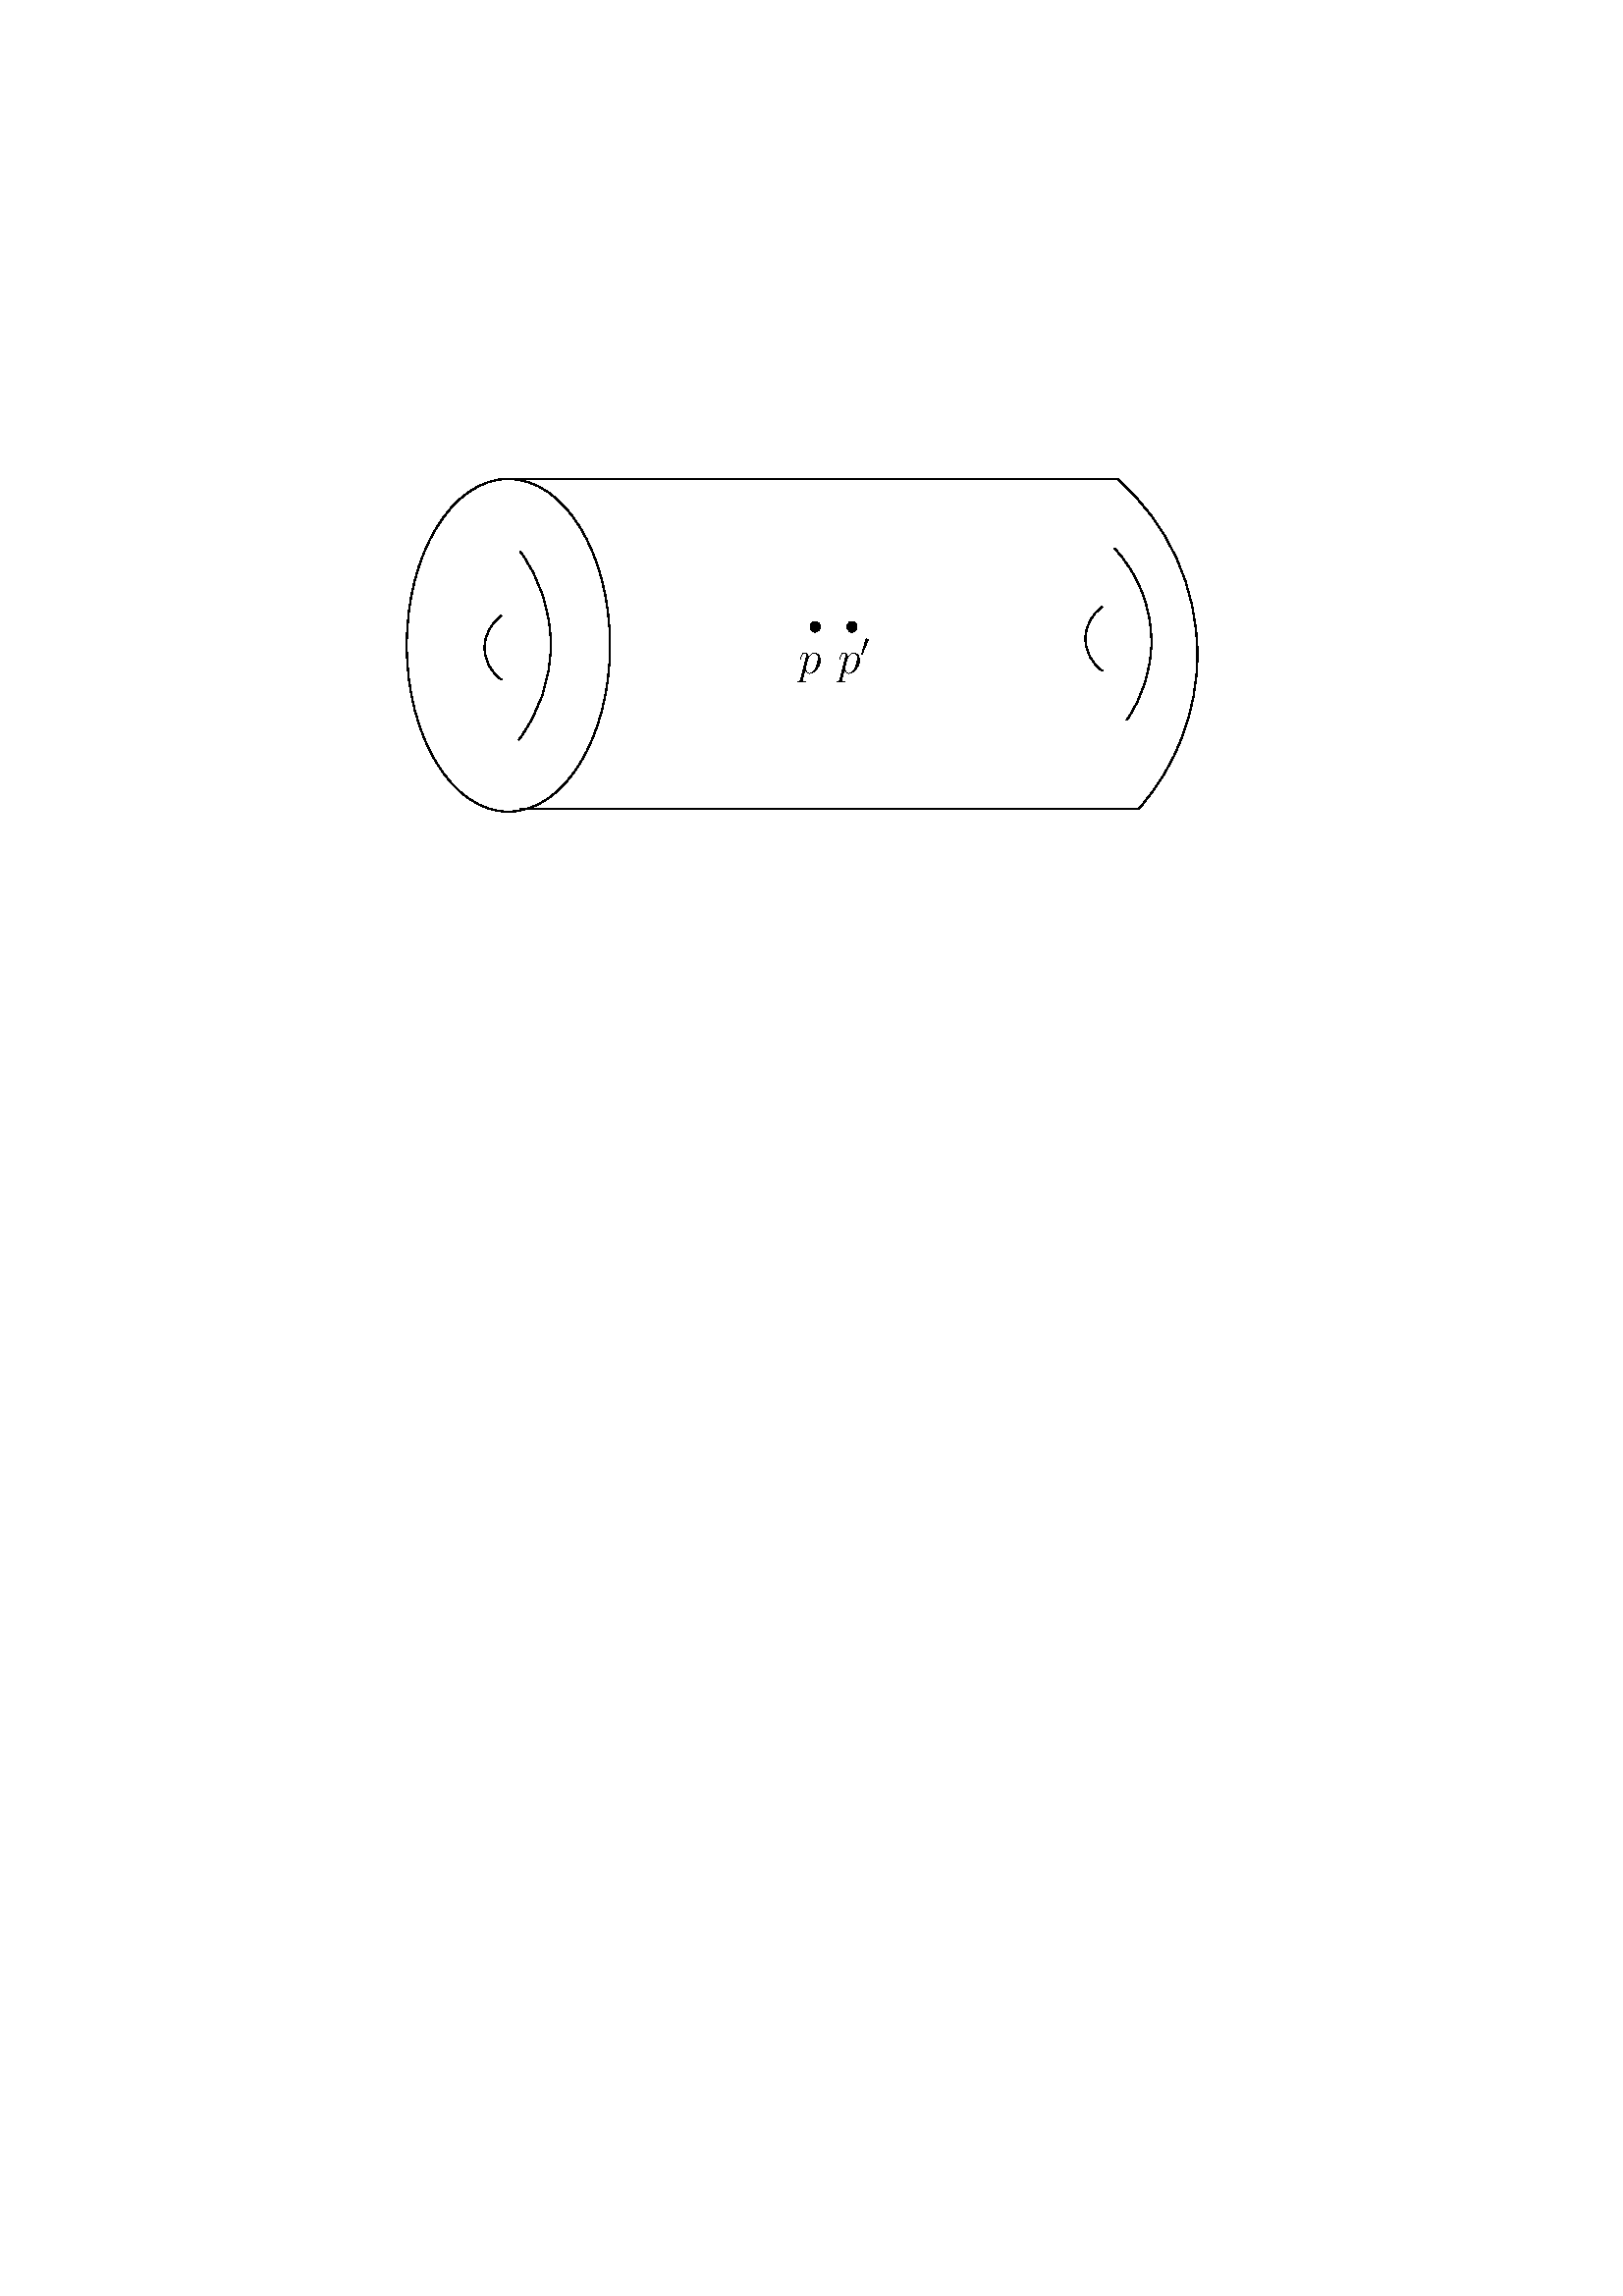
\includegraphics[width=0.75\linewidth]{figures/gla7-9.png}
\caption{A pair of Hecke modifications made at the same value of $z$ but at distinct points in $I$.（原文 Fig.~20）}
\label{fig:xytampo}
\end{figure}

但到此为止我们还没有说到任何依赖于加权射影空间奇点的地方。为看清奇点的作用，令 $^L\negthinspace w=(1/2,-1/2)$ 为对应于二维表示的权。相应的 Wilson 算子与自身的算子乘积展开应当读作
% 式 (10.31)
\setcounter{equation}{30}
\begin{equation}\label{eq:murtog}
T({}^L\negthinspace w)\cdot T({}^L\negthinspace
w)=T({}^L\negthinspace\bar w)\oplus T(0),
\end{equation}
 其中 $0$ 是零权，$T(0)=1$ 是相应的平凡 't Hooft 算子。（系数实际上是某个一维向量空间，但我们把它略去了。）让我们看看这是如何发生的。$^L\negthinspace w$ 型 Hecke 修正的空间同构于 $\Bbb{CP}^1$。若（\xytampo）我们在同一点 $z\in C$、但在 $I$ 中不同点处反复作 $^L\negthinspace w$ 型的 Hecke 修正，就得到模空间 $\bar\EUZ({}^L\negthinspace w,z,y;{}^L\negthinspace w,z,y')$，它是 $\Bbb{CP}^1$ 上的 $\Bbb{CP}^1$ 丛。其上同调是四维的，非零类出现在维数 $d=0,2,2,4$，故 $\EUK$ 的本征值为 $-2,0,0,2$。

现在让我们试着取 $y\to y'$ 的极限。对任意 $y<y'$，我们可以用 Hodge 理论；$\bar\EUZ$ 上调和形式的空间是四维的。在 $y=y'$ 处出现一个 $A_1$ 轨形奇点；局部结构看起来像 $\Bbb{R}^4/\Bbb{Z}_2$。当 $y$ 略小于 $y'$ 时（与区间 $I$ 的长度相比），这个奇点被消解。该消解可在局部用超凯勒流形 $\EUWW$（由 \cite{ref130} 发现）作为模型，它在一个复结构中可以等同于 $T^*\Bbb{CP}^1$。$\EUWW$ 上的度规是完备的，而且在无穷远处渐近于 $\Bbb{R}^4/\Bbb{Z}_2$ 上的平坦度规。

对我们至关重要的是，$\EUWW$ 上 ${\Bbb{L}}^2$ 调和形式的空间是一维的，由一个二形式 $\omega$ 生成 \cite{ref130}。（注意这里 ${\Bbb{L}}^2$ 条件涉及无穷远处的行为，而在相交上同调的定义中它涉及奇点附近的行为。）由于属于 ${\Bbb{L}}^2$，这个形式支撑在例外除子附近；当 $y\to y'$（例外除子收缩）时，它收敛为在奇点处有 delta 函数支撑的形式。它有 $d=2$，故对应于鬼数 $\EUK=0$ 的上同调类，而这个值对应于 $^L\negthinspace G=SU(2)$ 的平凡表示。$\EUWW$ 上这个 ${\Bbb{L}}^2$ 调和二形式之所以存在，是出于可用 \cite{ref131} 中论证理解的拓扑原因。

现在我们可以理解算子乘积关系 \eqref{eq:murtog} 的含义了。左端联系着反复 Hecke 修正的空间 $\bar\EUZ$。当 $y<y'$ 时，它是 $\Bbb{CP}^1$ 上的 $\Bbb{CP}^1$ 丛，有四维的调和形式空间，即物理 Hilbert 空间 ${\cal H}$。这个空间的一个三维子空间由这样的调和形式组成：它们当 $y\to y'$ 时收敛为 $\bar\EUZ{}^*=\Bbb{WCP}^2(1,1,2)$（即 $\bar\EUZ$ 在 $y\to y'$ 时的极限）光滑部分上的 ${\Bbb{L}}^2$ 调和形式。它们反映了 $T({}^L\negthinspace\bar w)$ 对 ${\cal H}$ 的贡献。第四个调和形式在 $y$ 接近 $y'$ 时可用 $\EUWW$ 上的 $\Bbb{L}^2$ 调和形式来近似，并且支撑在例外除子附近。这第四个调和形式的支撑当 $y\to y'$ 时收敛到 $\bar\EUZ{}^*$ 的奇点，而后者是权 $^L\negthinspace w=0$ 的 Hecke 修正空间。它是 $T(0)$ 对 ${\cal H}$ 的贡献。$T(0)$ 的系数为 1，这件事表达了：当 $y\to y'$ 时收敛到奇点的调和二形式空间恰好是一维的。更确切地说，$T(0)$ 的系数就是这个一维的调和形式空间。

更一般地，设给定任意一对权 $^L\negthinspace w$、$^L\negthinspace w'$。我们要描述算子乘积 $T({}^L\negthinspace w)\cdot T({}^L\negthinspace w')$，预期它具有如下形式
% 式 (10.32)
\setcounter{equation}{31}
\begin{equation}\label{eq:mitory}
T({}^L\negthinspace w)\cdot T({}^L\negthinspace
w')=T({}^L\negthinspace\,\bar w)\oplus\left(\oplus_{\alpha\in \EUR'}\,N_\alpha
\otimes T({}^L\negthinspace w_\alpha)\right),
\end{equation}
 其中 $^L\negthinspace\,\bar w={}^L\negthinspace w+{}^L\negthinspace w'$，求和遍历联系到 $^L\negthinspace\,\bar w$ 的各个权。当 $y\to y'$ 时，$\bar\EUZ({}^L\negthinspace w,y,z;{}^L\negthinspace w,y',z)$ 作为空间收敛到 $\bar\EUZ({}^L\negthinspace\,\bar w,y,z)$（后者对 $y$ 与 $z$ 的依赖无关紧要）。模空间上的一些 ${\Bbb{L}}^2$ 调和形式收敛为 $\bar\EUZ({}^L\negthinspace\,\bar w)$ 光滑部分上的这类形式。这些是 $T({}^L\negthinspace\,\bar w)$ 在算子乘积展开中的贡献。另一些则收敛为在 $\bar\EUZ({}^L\negthinspace w_\alpha)$（对 $^L\negthinspace\bar w$ 的某个伴随权 $^L\negthinspace w_\alpha$）上有 delta 函数支撑的形式。当 $y\to y'$ 时支撑在 $\bar\EUZ({}^L\negthinspace w_\alpha)$ 上、而不支撑在任何 $^L\negthinspace w_\alpha$ 的伴随权 $^L\negthinspace w_\beta$ 对应的 $\bar\EUZ({}^L\negthinspace w_\beta)$ 上的那些形式，就是 $T({}^L\negthinspace w_\alpha)$ 在算子乘积中的贡献。

最后，我们简要说明这一想法在数学上是如何表述的 \cite{ref97,ref98}。模空间 $\bar\EUZ({}^L\negthinspace w,z,y;{}^L\negthinspace w',z,y')$ 是纤维为 $\bar\EUZ ({}^L\negthinspace w',z,y')$、底为 $\bar\EUZ({}^L\negthinspace w,z,y)$ 的纤维化，正如我们在第~\ref{sec:kahstr}~节所解释的。当 $y\to y'$ 时，这个模空间被「坍缩」（blown down），以得到更奇异的空间 $\bar\EUZ({}^L\negthinspace\,\bar w,z,y')$，后者对 $z$ 与 $y'$ 的依赖无关紧要。这一坍缩是一个有理映射
% [WARN] 公式 \eqn\eqref{eq:normo} 无编号或重复
\begin{equation*}
\tag*{(10.33)}
\pi:\bar\EUZ({}^L\negthinspace w,z,y;{}^L\negthinspace
w',z,y')\to \bar\EUZ({}^L\negthinspace\,\bar w).
\end{equation*}

我们把 $\bar\EUZ({}^L\negthinspace w,z,y;{}^L\negthinspace w',z,y')$ 上的标准相交上同调复形记作 $IC({}^L\negthinspace w)\star IC({}^L\negthinspace w')$。（该记号的动机来自此空间的纤维丛结构。）相交上同调中有推下映射 $\pi_*$。由于层 $IC({}^L\negthinspace w)\star IC({}^L\negthinspace w')$ 在第~\ref{sec:affgrass}~节所谓的群 $GL(N,{\cal O})$（或其他 $G$ 对应的类似群 $G({\cal O})$）之下不变，而 $\pi_*$ 与该作用交换，所以推下 $\pi_*(IC({}^L\negthinspace w)\star IC({}^L\negthinspace w'))$ 同样在 $G({\cal O})$ 下不变。因此可以把它展开为 $\bar\EUZ({}^L\negthinspace\bar w)$ 的标准相交上同调复形 $IC({}^L\negthinspace\bar w)$ 与那些支撑在带权 $^L\negthinspace w_\alpha$（伴随于 $^L\negthinspace\bar w$）的奇异轨道上的复形 $IC({}^L\negthinspace w_\alpha)$ 之和。（这些是 $\bar\EUZ({}^L\negthinspace\bar w)$ 上仅有的 $G({\cal O})$-不变相交上同调复形。）

于是我们必须有\footnote{我们已把所有复形作维数平移，使其在正维数与负维数之间对称。映射 $\pi_*$ 保持这一对称性。因此我们不必担心进一步的平移。}
% 式 (10.34)
\setcounter{equation}{33}
\begin{equation}\label{eq:yrox}
\pi_*\left(IC({}^L\negthinspace w)\star
IC({}^L\negthinspace w')\right)=IC({}^L\negthinspace\bar
w)\oplus \left(\bigoplus_\alpha\, \tilde N_\alpha \otimes \,IC({}^L\negthinspace w_\alpha)\right).
\end{equation}
 首项 $IC({}^L\negthinspace\bar w)$ 的「系数」是平凡的一维向量空间（可以略去），因为映射 $\pi$ 在模空间的光滑部分上是同构。首项的这个性质在式~\eqref{eq:hffo} 的讨论中有初等的解释。其余的「系数」是向量空间 $\tilde N_\alpha$。这一表述类似于 't Hooft 算子乘积的一般结构 \eqref{eq:hffo}\ 或 \eqref{eq:zurgo}，其中相交复形 $IC({}^L\negthinspace w_\alpha)$ 代表 't Hooft 算子 $T({}^L\negthinspace w_\alpha)$ 的贡献。当然，证明 \cite{ref97,ref98} 的困难部分在于描述空间 $\tilde N_\alpha$，并建立它们与 \eqref{eq:omigron} 中出现的类似空间 $N_\alpha$ 的同构。

\begin{yizhu}[易错点]
按：本片反复出现的「系数」有两种，读时须分清。第~\ref{sec:lineop}~节用 $c$-数系数 $n_\alpha$ 写出的是 Wilson {\it 圈}算子的算子乘积展开（式~\eqref{eq:tryo}）；而静态 Wilson {\it 线}算子处理的是一段带边界的时间演化，其算子乘积展开 \eqref{eq:docus} 的系数是向量空间 $N_\alpha$ 而非整数。二者之间只差一个取迹：把时间方向紧致化为圆、对和乐取迹，$N_\alpha$ 就退化为它的维数 $n_\alpha$。这也解释了拓扑场论中圈算子算子乘积系数恒为整数的来源——那个整数其实是某个向量空间的维数。
\end{yizhu}

\begin{yizhu}[物理图像]
按：「一些有用的膜（Some Useful Branes）」一段的要点是：不必真的去量子化带 't Hooft 算子的四维规范理论，而应把边界条件翻译成二维 sigma 模型的膜。取 $B$ 支撑在 $\EUZ$ 上、固定全纯型 $E_-$ 而让 $\varphi$ 任意，取 $B'$ 支撑在 $\varphi=0$ 的那部分上，两膜横截于 $(E_-,0)$ 一点；于是超对称位形空间恰好就是 Bogomolny 模空间 $\EUZ$。时间分量 $\phi_0$ 在四维理论中是「有质量」的，在 sigma 模型中没有可供指定的边界条件，只能作为源出现在方程中——这正是本片开头要强调「选取合适的膜」的原因。
\end{yizhu}

\begin{yizhu}[易错点]
按：$\bar\EUZ$ 一般带有奇点（单极子冒泡的降权处），因此物理态空间不能取普通 de Rham 上同调，必须用相交上同调；后者（在标准猜想成立的前提下）可粗略地理解为光滑部分的 ${\Bbb{L}}^2$ 上同调，并作 $A$-模型式的维数平移 $\EUK=d-{\rm dim}_{{\Bbb C}}(X)$。物理上真正用到的性质是：$\bar\EUZ$ 的奇点结构不依赖于膜的位置 $p_i$，正因如此，才能用拓扑场论的论证说明 Hilbert 空间与 $p_i$ 无关，也才能把它当作一个只依赖边界条件的向量空间来用。
\end{yizhu}

\begin{yizhu}[物理图像]
按：$y\to y'$ 时出现 $A_1$ 轨形奇点 $\Bbb{R}^4/\Bbb{Z}_2$，它由超凯勒流形 $\EUWW$（Eguchi--Hanson 空间，在某些复结构下即 $T^*\Bbb{CP}^1$）解消；$\EUWW$ 上恰有一个 ${\Bbb{L}}^2$ 调和二形式 $\omega$，它支撑在例外除子附近，当例外除子收缩时收敛为奇点处的 delta 形式。$\omega$ 的次数为 $2$，故鬼数为 $0$，对应于 $^L\negthinspace G=SU(2)$ 的平凡表示，这正解释了 \eqref{eq:murtog} 中 $T(0)$ 的系数为何是 $1$。注意「${\Bbb{L}}^2$」在两处含义不同：在相交上同调的定义中它约束奇点附近的行为，而在 $\EUWW$ 上它约束的是无穷远处的行为。
\end{yizhu}

\begin{yizhu}[原文疑误]
按：「相应的 Wilson 算子与自身的算子乘积展开应当读作」一句，原文作 “the corresponding Wilson operator”，但紧随其后的式~\eqref{eq:murtog} 左端是 $T({}^L\negthinspace w)\cdot T({}^L\negthinspace w)$、右端首项是 $T(0)$，全段讲的都是 't Hooft 算子；Wilson 算子在这里只是作为电磁对偶的对照物出现。故此处应读作「相应的 't Hooft 算子」。译文照录原文的用词，并在此标出。
\end{yizhu}

\begin{yizhu}[易错点]
按：片中有两条单独成行的文献引用（分别指向相交同调理论的经典文献），位于「首先，该定理所用的上同调理论是相交上同调」之前。这是原文排版中的引用行，并非排版错误，已原样保留在两段之间，其命令与位置均未改动。
\end{yizhu}

\begin{yizhu}[含糊点拨]
按：数学上 \eqref{eq:yrox} 的推下与展开正是 Lusztig、Ginzburg、Mirković--Vilonen 的相交上同调卷积（即本片末尾所引的三项工作）：两两相交复形的卷积被推下后，按 $G({\cal O})$-不变性分解为各 $IC({}^L\negthinspace w_\alpha)$ 之和，系数即向量空间 $\tilde N_\alpha$。真正困难的部分不是这个分解形式，而是证明 $\tilde N_\alpha$ 同构于 \eqref{eq:omigron} 中的 $N_\alpha$——那才是几何 Satake 对应与张量积分解在数学上的等号内容。
\end{yizhu}

%% ============================================================
%% 分片 30：原文第 10 节「The Bogomolny Equations And The Space Of Hecke Modifications」（原文 glshort.tex 起于第 8120 行）
%% 由 tools/harvmac2tex.py 从 arXiv 源码（hep-th/0604151v3）自动生成。
%% 只译英文散文；公式、编号、\label、\cite 一律不改。
%% ============================================================

\subsection{扩展的 Bogomolny 方程}

\label{sec:extbog}

迄今为止，在研究 't Hooft 算子对膜的作用时，我们只考虑过不依赖于时间且时间反演不变的超对称解。在这一限制下，BPS 方程 \eqref{eq:oops}\ 约化为普通的 Bogomolny 方程，而 't Hooft 算子约化为通常的几何 Hecke 算子。

不依赖时间的假设其实一般来说是可以论证的，但要求时间反演不变性会对允许的边界条件施加严重限制。只有当我们挑选膜的方式（正如我们在第~\ref{sec:opprod}~节讨论 't Hooft 算子的乘积时所做的）能保证相关解满足 $\varphi=0$ 时，这个要求才是恰当的。对几何 Langlands 对偶而言最重要的那些 $A$-膜（Hitchin 纤维化的一般纤维，以及第~\ref{sec:abranes}~节所描述的 c.c. 膜），其支撑并不限于 $\varphi=0$；因此，为了研究 't Hooft 算子对它们的作用，我们需要放弃时间反演不变性这一条件。这正是下面讨论的目的。远为详尽的内容将另文给出 \cite{ref26}。

我们再次考虑四维流形 $M=\RR\times W$ 上的 BPS 方程，并把 Higgs 场 $\phi$ 写成 $\phi_0\, dx^0 +\pi^*\tilde\phi$，其中 $\pi$ 是到 $W$ 的投影，$\tilde\phi$ 是 $W$ 上的一形式 Higgs 场。同样，我们把规范场写成 $A=A_0\,dx^0+\tilde A$，其中 $\tilde A$ 是曲率为 $\tilde F$ 的三维联络。$t=1$ 时，不依赖于时间的 BPS 方程为
% 式 (10.35)
\setcounter{equation}{34}
\begin{equation}\label{eq:BPSstaticgen}
\begin{aligned}\tilde F-\tilde\phi\wedge\tilde\phi&=
\star\left(D\phi_0-[A_0,\tilde\phi]\right),\\ \star
D\tilde\phi&=[\phi_0,\tilde\phi]+D A_0,\\
D^*\tilde\phi+[A_0,\phi_0]&=0.\end{aligned}
\end{equation}
 这里外微分 $D$、Hodge 星算子 $\star$ 以及算子 $D^*=\star D\star$ 都按三维意义理解。

这些方程借助适当的消灭定理可以大大简化。事实上，用与时间反演不变情形相同的论证和同类型的假设（回忆式~\eqref{eq:wungo}），可以证明 $\phi_1=A_0=0$。

于是我们令 $\phi_1=A_0=0$，在 $C$ 上取局部复坐标 $z=x^2+ix^3$，记 $y=x^1$，并取规范 $\tilde A_y=0$。我们从此还把记号中的波浪号去掉。并且，正如第~\ref{sec:theck}~节的做法，我们取 $W$ 上的度规为 $ds^2=h |dz|^2+ dy^2$，其中 $h$ 是某个函数。于是扩展的 Bogomolny 方程 \eqref{eq:BPSstaticgen}\ 约化为
% 式 (10.36)
\setcounter{equation}{35}
\begin{equation}\label{eq:BPSextsimple}
\begin{aligned}D_\bz\phi_z&=0,\\
\partial_y A_\bz&=-i D_\bz \phi_0,\\
\partial_y\phi_z&=-i[\phi_z,\phi_0],\\
F_{z\bz}-[\phi_z,\phi_\bz]&={ih\over 2}\partial_y\phi_0.\end{aligned}
\end{equation}

\eqref{eq:BPSextsimple} 的第一式表明：对任意 $y\in I$，限制在 $C_y=\{y\}\times C$ 上的 $\varphi=\phi_z\,dz$ 是 $\End(E)\otimes K_C$ 的全纯截面。于是，若把由 $\bar\partial$ 算子 $\bar D=d\bar z(\partial_{\bar z}+A_{\bar z})$ 在 $C_y$ 上定义的全纯丛记作 $E$，则对任意 $y$，$(E,\varphi)$ 都是一个 Higgs 丛。接下来两式的解释，根据我们在第~\ref{sec:theck}~节处理普通 Bogomolny 方程的经验，应当不难预料：它们说的是，沿 $y$ 方向的演化只以规范变换的方式改变 Higgs 对 $(E,\varphi)$。因此，在遇到与 't Hooft 算子相联系的奇点之前，扩展 Bogomolny 方程的一个解所决定的 $\MH$ 中的点与 $y$ 无关。

现在设有一个权为 $^L\negthinspace w$ 的 't Hooft 算子，位于（比方说）$y=y_0$、$z=z_0$。当 $y$ 增大越过 $y=y_0$ 时，丛 $E$ 经历一次普通的 Hecke 修正，正如第~\ref{sec:theck}~节所描述的那样。事实上，$A_{\bar z}$ 的演化方程与第~\ref{sec:theck}~节中的相同，由 't Hooft 算子引起的奇点也相同。对 $(E,\varphi)$ 同样发生我们将称为 Hecke 修正的变化。然而 $\varphi$ 的作用与 $E$ 的作用大不相同。

全纯丛可以在单个点上被修正而保持全纯性，Hecke 算子或 't Hooft 算子所做的正是这件事。这种可能的修正构成一个模空间，即大家熟悉的、参数化 Bogomolny 方程奇异解的空间 $\bar {\EUY}({}^L\negthinspace w;z_0)$（它同构于一个 Schubert 簇）。但一个全纯场——在此情形是 ${\rm ad}(E)\otimes K_C$ 的全纯截面 $\varphi$——不能在一点被修正而保持全纯性。因此，如果 $\varphi$ 在 $z=0$ 之外给定，那么越过 $z=0$ 它至多只有唯一一个全纯延拓。

所以，把 $\varphi$ 包括进来，并不会使 't Hooft 算子引起的 Hecke 修正依赖于额外的参数。恰恰相反，一般地，包括 $\varphi$ 会消去一些参数。原因在于：即使 $\varphi$ 在 $y<y_0$ 时于 $z=z_0$ 处全纯，在 $y>y_0$ 时它一般也会在 $z=z_0$ 处出现极点。为看清这一点，我们取 $G=U(N)$，考虑权为 $^L\negthinspace w=(m_1,\ldots,m_N)$ 的 't Hooft 算子。越过 $y=y_0$ 时丛 $E$ 的全纯型发生跳变；我们把「之前」与「之后」的丛分别记为 $E_-$ 和 $E_+$。相对于某个局部分解 $E_-\cong \oplus_{i=1}^N \cL_i,$ 丛 $E_+$ 有局部分解 $\oplus_{i=1}^N\cL_i\otimes \CO(z_0)^{m_i}$。也就是说，若 $\cL_i$ 局部由全纯截面 $s_i$ 生成（$i=1,\ldots,N$），则 $E_+$ 由全纯截面 % 式 (10.37)
\setcounter{equation}{36}
\begin{equation}\label{eq:zilfog}
t_i=(z-z_0)^{-m_i} s_i.
\end{equation}
 这里我们对 $z\neq 0$ 利用了 $E_+$ 与 $E_-$ 之间的一个自然同构。

设 $\varphi$ 在 $y<y_0$ 时于 $z_0$ 处全纯。乘积 $\varphi \,s_i$ 是 $E_- \otimes K_C$ 的全纯截面（因为可以在 $z=z_0$ 附近把它平凡化，$K_C$ 在此不起本质作用），故可按 $s_i$ 展开：
% 式 (10.38)
\setcounter{equation}{37}
\begin{equation}\label{eq:bongo}
\varphi\cdot s_i=\sum_j f_i{}^j\,s_j.
\end{equation}
  $\varphi$ 在 $y<y_0$ 时于 $z=z_0$ 处全纯，这一事实说明 $f_i{}^j$（它们是 $K_C$ 的截面）在 $z=z_0$ 处全纯。它们不再受其他约束。

同样，对 $y>y_0$，我们可以把 $\varphi\,t_i$ 展开为 $t_j$ 的线性组合。给定 $s_i$ 与 $t_i$ 之间的关系 \eqref{eq:zilfog}\ 后，我们可以立即写出展开式的形式： % 式 (10.39)
\setcounter{equation}{38}
\begin{equation}\label{eq:bzongo}
\varphi\cdot t_i=\sum_j
(z-z_0)^{m_j-m_i}f_i{}^j\,t_j.
\end{equation}
 要使 $\varphi$ 在 $y>y_0$ 时全纯，函数 $(z-z_0)^{m_j-m_i}f_i{}^j$ 必须在 $z=z_0$ 处全部正则。若把 $m_i$ 按通常方式排序为 $m_1\geq m_2\geq\dots\geq m_N$，则对 $f_i{}^j$ 在 $z=z_0$ 附近的 Taylor 级数系数所要施加的条件数目为 $\sum_{i<j}(m_i-m_j)$。

这与式~\eqref{eq:ydro} 所确定的丛的 Hecke 修正空间的维数相同。这强烈提示：与丛的 Hecke 修正情形形成鲜明对照，Higgs 丛 $(E,\varphi)$ 的 Hecke 修正一般构成有限集。事实上，只要 $\varphi(z_0)$ 正则且半单（对 $G=U(N)$ 而言即它可对角化且本征值互异），情形就是如此。对结果最系统的描述是：$\varphi$ 在参数化 $E$ 于 $z_0$ 处 $^L\negthinspace w$ 型 Hecke 修正的簇 $\bar {\EUY}({}^L\negthinspace w,z_0)$ 上确定一个向量场；该向量场的零点就是 $(E,\varphi)$ 的可能的 Hecke 修正。（这个向量场并不完全由典范方式确定，但它的零点是。）

把详细解释留待 \cite{ref26}，我们简要描述 $G=U(2)$、$^L\negthinspace w=(1,0)$ 的例子。在这个例子中，正如我们在第~\ref{sec:spaceheck}~节所学到的，若取丛 $E_-$ 为平凡丛，则 $E_+$ 可以这样刻画：$E_+$ 在 $z=0$ 处全纯的截面具有形式 % 式 (10.40)
\setcounter{equation}{39}
\begin{equation}\label{eq:hxonxno}
s_+=(z-z_0)^{-1}
u+(h_1(z),h_2(z)),
\end{equation}
  其中 $u$ 是 $\Bbb{C}^2$ 的某个非零元素，$h_1$ 与 $h_2$ 在 $z=z_0$ 附近全纯。在模去 $\Bbb{C}^*$ 的伸缩后，$u$ 参数化了 $E$ 的可能的 Hecke 修正所构成的空间，在本例中它就是 $\Bbb{CP}^1$。$\varphi$ 在 $y>y_0$ 时于 $z=z_0$ 处全纯，当且仅当乘积 $\varphi\cdot s_+$ 具有同样的形式，换言之，当且仅当 $\varphi u$ 是 $u$ 的倍数。在正则半单情形，这意味着 $u$ 必须是 $\varphi$ 的两个特征向量之一。

回到扩展的 Bogomolny 方程 \eqref{eq:BPSextsimple}，由关系 $\partial_y\phi_z=-i[\phi_z,\phi_0]$ 立即得到：若 $\phi_z$ 在某个 $y$ 处为零，则它处处为零。我们在第~\ref{sec:opprod}~节分析 't Hooft 算子的乘积时假设了这一点。同一方程的又一个推论是：$\varphi$ 的特征多项式与 $y$ 无关，即使在越过一个 't Hooft 算子时也是如此。因此，Higgs 丛的 Hecke 变换把 Hitchin 纤维化的每根纤维映入它自身。

现在考虑一根缠在 Hitchin 纤维化某根纤维上、并带有平坦 Chan-Paton 丛的膜。按照 $S$-对偶，这类膜必是磁特征膜。由上一段所述，这种膜的支撑在 Hecke 变换下不变。这一观察是向着不依赖 $S$-对偶而直接证明这类膜是磁特征膜迈出的一步，细节将另文给出 \cite{ref26}。

\par\medskip{\it Higgs 丛的 Hecke 对应}

正如我们在讨论普通 Bogomolny 方程时那样，我们可以考虑给定 Higgs 丛 $(E,\varphi)$ 的可能的 Hecke 修正——这也是我们迄今的观点——也可以更对称地描述初态与末态，即描述 Higgs 丛空间上的一个 Hecke 对应 ${\EUQ}$。我们这样来定义 ${\EUQ}$：在 $W=I\times C$ 上求解扩展 Bogomolny 方程，在两端取适当的边界条件，并在指定 't Hooft 算子的存在下求解。我们在 $W$ 的两端同时指定 $A$ 与 $\varphi$（但不指定 $\phi_0$），并且只模去在每一端均为平凡的规范变换。

设 $\EUW_0$ 为 $C$ 上满足 $\bar D\varphi=0$ 的规范场与 Higgs 场构成的全体对 $(A,\varphi)$ 的空间。那么 $\EUW_0$ 就是全体 Higgs 丛的「栈（stack）」${\rm Higgs}_G$ 的规范场论版本，正如全体联络的空间是全体 $G$-丛的栈 ${\rm Bun}_G$ 的规范场论版本。把扩展 Bogomolny 方程的解限制到其边界值，${\EUQ}$ 便有一对到 $\EUW_0$ 的映射，换言之，一个到 $\EUW_0\times \EUW_0$ 的映射。这就是 Higgs 丛的 Hecke 对应。

${\EUQ}$ 一般而言非常复杂，具有各种不同维数的分支。然而，如果只限于 $\EUW_0$ 的一个良好区域（其中每个 Higgs 丛在模去规范变换后只有有限多个给定类型的可能 Hecke 修正），那么 ${\EUQ}$ 可视为 $\EUW_0\times \EUW_0$ 的子流形。此外，在这个良好区域中我们可以模去规范变换，${\EUQ}$ 就成为 $\MH\times\MH$ 的中间维数子流形。

't Hooft 算子保持 $(B,A,A)$ 型超对称，正如我们在第~\ref{sec:lineop}~节末所解释的。这意味着必须能把 ${\EUQ}$ 解释为 $\MH\times \MH$ 中的 $(B,A,A)$ 型膜。特别地，它必须在复结构 $I$ 中全纯，并且相对于复结构 $J$ 与 $K$——等价地，相对于式~\eqref{eq:ninto} 所定义的全纯辛形式 $\Omega_I=\omega_J+i\omega_K$——是拉格朗日的\footnote{在中间维数以上，存在不是拉格朗日的 $A$-膜 \cite{ref80}。但在良好区域中，${\EUQ}$ 是中间维数的，故必是拉格朗日的。}。更确切地说，若 $\pi_i:{\EUQ}\to\MH\times\MH$（$i=1,2$）是两个投影，则 ${\EUQ}$ 必须相对于 $\MH\times \MH$ 上的全纯辛形式 $\Omega=\pi_1^*(\Omega_I)-\pi_2^*(\Omega_I)$ 是拉格朗日的。这里的负号保证了 $\MH\times \MH$ 中的对角——即没有 't Hooft 算子的平凡 Hecke 对应——是拉格朗日的。

记 $C_+$ 与 $C_-$ 为 $W=I\times C$ 的两端，我们可以把 $\Omega$ 在 ${\EUQ}$ 上的限制写成
% 式 (10.41)
\setcounter{equation}{40}
\begin{equation}\label{eq:symplevolume}
{1\over\pi}\left(\int_{C_+}
-\int_{C_-}\right)|d^2 z|\,\Tr\left(\delta\phi_z\wedge \delta
A_\bz\right)={1\over \pi}\int_Idy\int_C|d^2z|\,
\partial_y \Tr\left(\delta\phi_z\wedge\delta A_\bz\right).
\end{equation}

为计算这个形式在 $\EUQ$ 上的限制，我们可以假定变分 $\delta\phi_z$ 与 $\delta A_\bz$ 满足 \eqref{eq:BPSextsimple}\ 的线性化。\eqref{eq:BPSextsimple}\ 中前三式的线性化给出
% 式 (10.42)
\setcounter{equation}{41}
\begin{equation}\label{eq:BPSlin}
\begin{aligned}D_\bz\delta\phi_z&=-[\delta
A_\bz,\phi_z],\\
\partial_y\delta A_\bz&=-iD_\bz\delta\phi_0 - i [\delta
A_\bz,\phi_0]\\
\partial_y\delta\phi_z&=-i[\delta\phi_z,\phi_0]-i[\phi_z,\delta\phi_0]
.\\\end{aligned}
\end{equation}
 利用这些方程、Jacobi 恒等式以及分部积分，可以验证 \eqref{eq:symplevolume}\ 为零，因此 ${\EUQ}$ 如预期的那样是复拉格朗日的。

\begin{yizhu}[原文疑误]
按：本片有一处 $z=0$ 照录原文，实应为 $z=z_0$。原文说“若 $\varphi$ 在 $z=0$ 之外给定，则越过 $z=0$ 它至多只有唯一一个全纯延拓”，但全段讨论的 't Hooft 算子位于 $z=z_0$，奇点空间也记作 $\bar {\EUY}({}^L\negthinspace w;z_0)$；紧随其后的段落写“即使 $\varphi$ 在 $y<y_0$ 时于 $z=z_0$ 处全纯……在 $y>y_0$ 时它一般也会在 $z=z_0$ 处出现极点”，可见前两处 $z=0$ 是 $z=z_0$ 的笔误。照录并标出，读者按 $z=z_0$ 理解即可，数学内容不受影响。
\end{yizhu}

\begin{yizhu}[易错点]
按：不要把 \eqref{eq:BPSstaticgen}\ 与第~\ref{sec:theck}~节的普通 Bogomolny 方程混为一谈：普通情形靠时间反演不变性可以证明 $\phi_1=A_0=0$，只剩 $W$ 上的方程；而“扩展”情形只是令 $t=1$、保留时间分量 $\phi_0$ 与 $A_0$ 作为待解的场，方程 \eqref{eq:BPSstaticgen}\ 中的 $D$、$\star$、$D^*=\star D\star$ 都是三维 $W$ 上的算子，$A_0$、$\phi_0$ 以“源”的形式出现在右端（如 $\partial_yA_{\bar z}=-iD_{\bar z}\phi_0$）。只有再借助消灭定理才可令 $\phi_1=A_0=0$，得到 \eqref{eq:BPSextsimple}。
\end{yizhu}

\begin{yizhu}[易错点]
按：本片最反直觉的一点是：丛的 Hecke 修正带参数（模空间 $\bar {\EUY}({}^L\negthinspace w;z_0)$ 的维数为 $\sum_{i<j}(m_i-m_j)$），而把 $\varphi$ 一起纳入后修正反而“消去参数”、一般只有有限多个。原因是对比的对象不同：全纯丛可以在单点被扭化而保持全纯（这正是 Hecke 修正），而全纯截面不能在单点修改还保持全纯，所以 $\varphi$ 在 $y>y_0$ 侧的全纯性对 $f_i{}^j$ 的 Taylor 系数施加了恰好 $\sum_{i<j}(m_i-m_j)$ 个条件——数目与丛的修正空间维数相同。当 $\varphi(z_0)$ 正则半单时该向量场零点有限，故可能的 Hecke 修正构成有限集。
\end{yizhu}

\begin{yizhu}[物理图像]
按：可把 $\varphi$ 想成 Schubert 簇 $\bar {\EUY}({}^L\negthinspace w,z_0)$ 上的一个向量场，其零点就是“允许的”修正；这比逐条数 Taylor 系数更几何。更关键的物理后果是特征多项式与 $y$ 无关，即使越过 't Hooft 算子也不变，故 $\varphi$ 所在的 Hitchin 纤维被保持：缠在 Hitchin 纤维上的膜（带平坦 Chan-Paton 丛者）在 Hecke 变换下支撑不变。这正是“磁特征膜”的直观内容，也是本片末尾要在 $\MH\times\MH$ 上构造 Hecke 对应 ${\EUQ}$ 的动机。
\end{yizhu}

\begin{yizhu}[易错点]
按：$\Omega=\pi_1^*(\Omega_I)-\pi_2^*(\Omega_I)$ 中的负号不是任意约定。限制到对角 $\Delta\subset\MH\times\MH$ 上，两项相消给出 $0$，于是平凡 Hecke 对应（无 't Hooft 算子）的支撑是拉格朗日的；若换成加号，拉回将是 $2\Omega_I$，对角就辛而非拉格朗日。另外 $(B,A,A)$ 型的读法是：在复结构 $I$ 中全纯（$B$ 的首字母），在 $J$、$K$ 中均为 $A$-型（即相对于 $\Omega_I=\omega_J+i\omega_K$ 拉格朗日）；\eqref{eq:symplevolume}\ 的验证只用到 \eqref{eq:BPSextsimple}\ 的线性化、Jacobi 恒等式与分部积分，故 ${\EUQ}$ 在该良好区域确实是复拉格朗日的。
\end{yizhu}

%% ============================================================
%% 分片 31：原文第 11 节「$A$-膜与 ${\cal D}$-模」（原文 glshort.tex 起于第 9938 行）
%% 由 tools/harvmac2tex.py 从 arXiv 源码（hep-th/0604151v3）自动生成。
%% 只译英文散文；公式、编号、\label、\cite 一律不改。
%% ============================================================

\section{$A$-膜与 ${\cal D}$-模}
\label{sec:abranes}

\begin{keytakeaways}
  \begin{itemize}[leftmargin=1.4em,itemsep=2pt,topsep=2pt]
    \item \textbf{物理图像}：几何 Langlands 对应的左端已知是电特征膜（即 $\pi_1(C)\to{}^L\negthinspace G$ 的同态），其对偶是缠在 Hitchin 纤维上、带平坦 Chan-Paton 丛的磁特征膜；但通常表述的右端并不是 $\MH$ 上的 $(A,B,A)$ 型膜，而是 $G$-丛模空间上的 ${\cal D}$-模。本节的物理任务就是补上这最后一段翻译。
    \item \textbf{数学工具}：${\cal D}$-模是微分算子层的模；把 $\M(G,C)$ 上的 ${\cal D}$-模看成其余切丛的非交换形变上的 $B$-膜，则 $A$-膜的范畴与这类 $B$-膜范畴的等价（原文引 Kapustin 的论证）使「$A$-膜给出 ${\cal D}$-模」成为该等价的一个特例。
    \item \textbf{关键结论}：$\MH(G,C)$ 上复结构 $K$ 中的每个 $A$-膜都自动给出（粗略地说）$\M(G,C)$ 上的一个 ${\cal D}$-模；这就是所谓 A-膜到 D-模的翻译器，是几何 Langlands 纲领与规范理论对偶之间缺失的一环。
    \item \textbf{边界与展望}：严格处理不能只停留在稳定丛的模空间 $\M(G,C)$，而要在所有 $G$-丛的叠 ${\rm Bun}_G(C)$ 上构造 ${\cal D}$-模（Hecke 算子的作用方式要求如此）；相应地，所关心的膜必须能在底层规范理论中定义，而不只是在靶空间为 $\MH(G,C)$ 的 sigma 模型中定义，这一点在第~\ref{sec:zapendix}~节证明。
  \end{itemize}
\end{keytakeaways}


迄今所讲的内容还缺一个关键要素。按照几何 Langlands 纲领，$\pi_1(C)$ 到 $^L\negthinspace G$ 的同态与 ${\EUM}(G,C)$ 上的 Hecke 特征层之间存在自然的对应，而这些特征层同时也是 ${\cal D}$-模。所谓 ${\cal D}$-模，就是微分算子层的模；这个概念下面还会进一步说明。

至于对应式的左端，我们在第~\ref{sec:electricbranes}~节已经知道：$\pi_1(C)$ 到 $^L\negthinspace G$ 的同态对应于电特征膜。它们的对偶因此必定是磁特征膜；这些对偶是 ${\CMF}$ 型膜，即缠在 Hitchin 纤维化的一条纤维上、带平坦 Chan-Paton 丛的膜。这一陈述可由 $S$-对偶得到，也可以借助谱覆盖构造所提供的阿贝尔化直接验证 \cite{ref26}。

然而，这样得到的磁特征膜是 $\MH(G,C)$ 上的 $(A,B,A)$ 型膜；而在几何 Langlands 对应的通常表述中，右端应当涉及的却是（粗略地说）$G$-丛的模空间 $\M(G,C)$ 上的 ${\cal D}$-模。

本节的任务就是补上这缺失的一环。我们将证明：$\MH(G,C)$ 上复结构 $K$ 中的每一个 $A$-膜都自动给出（粗略地说）$\M(G,C)$ 上的一个 ${\cal D}$-模。

人们可以把 $\M(G,C)$ 上的 ${\cal D}$-模看作 $\M(G,C)$ 的余切丛的非交换形变上的 $B$-膜。此前已有论证 \cite{ref41}：对某一类全纯辛流形，$A$-膜的范畴等价于同一流形的非交换形变上 $B$-膜的范畴。$\MH(G,C)$ 上的 $A$-膜与 $\M(G,C)$ 上的 ${\cal D}$-模之间的联系，可以看作这一点的一个特例。

事实上，在几何 Langlands 纲领中，只在稳定丛的模空间 $\M(G,C)$ 上工作是不够的（而且由于 Hecke 算子的作用方式，也不可能这样做）。人们改而在 $C$ 上所有 $G$-丛构成的「叠」 ${\rm Bun}_G(C)$ 上构造 ${\cal D}$-模。所有 $G$-丛构成的叠在规范理论中的类比物，就是所有联络构成的空间。通常的说法是「${\cal D}$-模定义在 ${\rm Bun}_G(C)$ 上」；在我们的构造中与之对应的说法是：所关心的膜可以在底层的规范理论中定义，而不只是在靶空间为 $\MH(G,C)$ 的 sigma 模型中定义。对重要的膜证明这一点，实际上正是第~\ref{sec:zapendix}~节的目标。

\begin{yizhu}[含糊点拨]
按：本片两处「粗略地说」（roughly speaking）值得留意。一处修饰「$\M(G,C)$ 上的 ${\cal D}$-模」：严格的对象其实是 ${\rm Bun}_G(C)$ 上的（扭化）${\cal D}$-模，只因 Hecke 算子会把稳定丛变出稳定丛之外，才不能只停在 $\M(G,C)$ 上。另一处修饰「每个 $A$-膜都自动给出一个 ${\cal D}$-模」：翻译器的精确定义还要选取合适的 $A$-膜范畴（含余各向同性的对象）并对 ${\cal D}$-模作相应的扭化，所以原文才说「粗略地说」。
\end{yizhu}

\begin{yizhu}[易错点]
按：本片出现三个容易混淆的空间：$\MH(G,C)$ 是超凯勒的 Hitchin 模空间，膜（包括磁特征膜）住在这里，其复结构 $K$ 中的 $A$-膜是本片的主角；$\M(G,C)$ 是稳定 $G$-丛的模空间，${\cal D}$-模粗略地说住在这里；${\rm Bun}_G(C)$ 则是所有 $G$-丛构成的叠，才是 ${\cal D}$-模严格的家。镜像对称的三角中三条边分别是：$\MH({}^L\negthinspace G)$ 上的 $A$-膜、$\MH(G,C)$ 上的 $B$-膜、以及 ${\rm Bun}_G(C)$ 上的 ${\cal D}$-模；本片补的正是「$A$-膜 $\to$ ${\cal D}$-模」这一条边。
\end{yizhu}

\begin{yizhu}[物理图像]
按：把 ${\cal D}$-模想成余切丛上的 $B$-膜是理解本片的关键：$\M$ 的局部坐标 $x^i$ 与其对偶 $p_i$ 若实现为 $x^i$ 与 $\partial/\partial x^i$，就不再对易，于是 $T^*\M$ 变成一个非交换空间，而 ${\cal D}$-模恰是它上面的「$B$-膜」。$\MH$ 包含 $T^*\M^{st}$ 作为 Zariski 开集，因此 $\MH$ 上的 $A$-膜与 $\M$ 上的 ${\cal D}$-模之间的关系自然被期待为「同一块非交换几何的两个侧面」；本片正是把这一期待落实为具体构造的起点。
\end{yizhu}

\begin{yizhu}[物理图像]
按：「所有 $G$-丛构成的叠」在规范理论中的类比物是「所有联络构成的空间」，这句话解释了对偶为什么必须离开半稳定丛：'t Hooft 算子（Hecke 算子）在四维规范理论中作用于所有联络，而不只作用于满足稳定性条件的解；因此「${\cal D}$-模定义在 ${\rm Bun}_G(C)$ 上」这一数学事实，对应的是「所关心的膜可以在底层规范理论中定义，而不只是在靶空间为 $\MH(G,C)$ 的 sigma 模型中定义」。
\end{yizhu}

\begin{yizhu}[含糊点拨]
按：原文说 $A$-膜范畴与「某类全纯辛流形的非交换形变上 $B$-膜范畴」的等价「此前已有论证」，这是指 Kapustin 关于 A-膜与非交换几何的工作（本片此处的引用即该文）。注意原文用的动词是「argued（论证）」而非「proved（证明）」：这一等价在原文写作时还只是物理论证，并非定理；若读者要引用严格结果，须另找关于这类范畴等价的数学文献。
\end{yizhu}

%% ============================================================
%% 分片 32：原文第 11 节「$A$-Branes and ${\cal D}$-Modules」（原文 glshort.tex 起于第 9938 行）
%% 由 tools/harvmac2tex.py 从 arXiv 源码（hep-th/0604151v3）自动生成。
%% 只译英文散文；公式、编号、\label、\cite 一律不改。
%% ============================================================

\subsection{典范余各向同性 $A$-膜}

我们的出发点是 \cite{ref80} 中的一个观察：对一般的辛流形 $X$，可能存在
不支撑在 Lagrange 子流形上、而支撑在更一般的余各向同性子流形上的
$A$-膜。辛流形 $X$ 的余各向同性子流形 $Y$ 是指局部由第一类约束定义的
子流形；换言之，它局部由若干 Poisson 对易的函数 $f_i$，$i=1,\dots,d$
的零点集定义。$X$ 上独立的 Poisson 对易函数的最大数目是 $X$ 维数的一半，
所以 $Y$ 的维数至少是 $X$ 维数的一半。若 $Y$ 的维数恰好是 $X$ 维数的
一半，则 $Y$ 是 Lagrange 的，而支撑在 $Y$ 上的 $A$-膜就是通常的
Lagrange $A$-膜。支撑维数高于中维的余各向同性 $A$-膜一般也存在，不过
它们存在的条件相当特殊。

我们只需要 $Y=X$ 且 $A$-膜秩为一的情形。于是其 Chan-Paton 丛是
$U(1)$ 丛 ${\cal L}\to X$。Chan-Paton 规范场取值于 $U(1)$ 的李代数，
而这是一个一维实向量空间。因此该规范场局部就是普通的实一形式 $A$，
其协变微分为 $D=d+A$；曲率定义为 $F=dA$。在 $U(1)$ 的酉表示中，
李代数 $\frak{u}(1)$ 的元素 $1$ 通过 $1\times 1$ 的反厄米矩阵 $-in$
作用，$n$ 为某个整数，而平行移动为 $\exp(in\int A)$。我们把 $X$ 上的
Chan-Paton 丛解释为与表示 $n=1$ 相伴的线丛。对 sigma 模型的映射
$\Phi:\Sigma\to X$，世界面路径积分中与 Chan-Paton 丛相关的因子，是
$\Phi^*(A)$ 沿 $\partial\Sigma$ 在 $n=1$ 表示中的和乐（holonomy），即
$\exp(i\oint_{\partial\Sigma}\Phi^*(A))$。

对一个 $Y=X$、Chan-Paton 线丛为 ${\cal L}$ 的膜，要成为 $A$-膜，其曲率
$F$ 必须满足
% 式 (11.1)
\setcounter{equation}{0}
\begin{equation}\label{eq:coisobrane}
(\omega^{-1}F)^2=-1.
\end{equation}
 也就是说，$(1,1)$ 张量 $\omega^{-1}F$ 是一个近复结构。形式 $F$ 与
$\omega$ 都是闭的，与 \eqref{eq:coisobrane} 一起可推出近复结构
$\hat N=\omega^{-1}F$ 是可积的 \cite{ref80}。容易看出，$\omega$ 与 $F$
关于 $\hat N$ 都是 $(2,0)\oplus(0,2)$ 型的。此外，复形式 $\omega-iF$
是 $(2,0)$ 型的，因而是 $X$ 上的一个全纯辛形式。所以这类余各向同性
$A$-膜只有在 $\omega$ 是某个全纯辛形式的实部时才可能存在。关于在
广义复几何中构造这类膜，另见 \cite{ref67}。

我们感兴趣的是 $\MH(G,C)$ 上辛结构为 $\omega=(\Im\tau)\,\omega_K$ 的
$A$-模型。此时式 \eqref{eq:coisobrane} 有一个显然的解： % 式 (11.2)
\setcounter{equation}{1}
\begin{equation}\label{eq:yetro}
F=
(\Im\tau)\,\omega_J,\quad \hat N=\omega_K^{-1}\omega_J= I.
\end{equation}

（也存在把 $F$ 与 $\hat N$ 的符号反过来的第二个解。）二形式 $\omega_J$
是恰当的，正如我们在第~\ref{sec:mhhyper}~节中所解释的，所以 $F$ 是平凡
线丛 ${\cal N}\to\MH(G,C)$ 上某个联络的曲率二形式。联络形式为 % 式 (11.3)
\setcounter{equation}{2}
\begin{equation}\label{eq:exactcc}
\alpha={\Im\tau\over {2\pi}}\int_C |d^2z|\,
\Tr \left(\phi_z\delta A_\bz +\phi_\bz \delta A_z\right)
\end{equation}
 且 $F=d\alpha$。虽然更一般的二形式 % 式 (11.4)
\setcounter{equation}{3}
\begin{equation}\label{eq:lombo}
(\Im\tau)\left(a\omega_J+b\omega_I\right), \quad a^2+b^2=1,
\end{equation}
 也满足式 \eqref{eq:coisobrane}，但它在 $b\neq 0$ 时不是恰当的，
并且对一般的 $\tau$ 值，其周期不是 $2\pi$ 的整数倍。所以在一般情况下，
这个形式不是任何联络的曲率二形式，不能用来构造 $A$-膜。

我们把 $\MH$ 上满足 $F=(\Im\tau)\,\omega_J$ 的 $A$-膜称为典范余各向同性
膜，简称 c.c. 膜。我们有时也把它记作 ${\cal B}_{c.c.}$。若 $G$ 单连通，
则 $\MH(G,C)$ 也单连通，此时 c.c. 膜是唯一的；否则，它唯一到把其
Chan-Paton 丛扭化一个平坦线丛为止。

关于 c.c. 膜的第一个观察是：它是一个 $(A,B,A)$-膜，即在复结构 $I$ 与
$K$ 中是 $A$-膜、在复结构 $J$ 中是 $B$-膜。要验证它在复结构 $I$ 中是
$A$-膜，我们只需要恒等式
% [WARN] 公式 \eqn\eqref{eq:hombo} 无编号或重复
\begin{equation*}
\tag*{(11.5)}
(\omega_I^{-1}\omega_J)^2=-1.
\end{equation*}
 这意味着 c.c. 膜在复结构 $I$ 中满足余各向同性膜的条件，正如它在复结构
$K$ 中一样。要验证它在复结构 $J$ 中是 $B$-膜，只需注意膜上规范场的曲率
是 $\omega_J$ 的倍数，而 $\omega_J$ 在复结构 $J$ 中是 $(1,1)$ 型的。

这些公式其实只在 $\MH$ 的光滑部分定义了 c.c. 膜。不过，c.c. 膜可以由
底层规范理论中的边界条件来定义；详见第~\ref{sec:xgoto}~节。这一论断在
量子场论上等价于说：该构造在整个 $G$-丛的「栈」上都成立。

接下来，我们想理解两端都落在 c.c. 膜上的拓扑开弦。它们由 BRST 不变的
边界算子插入来代表。一般而言，正如我们在第~\ref{sec:comptwo}~节 的
\dunamp\ 中所概述的，对任何膜 ${\cal B}$，$({\cal B},{\cal B})$ 弦构成
一个结合代数（但未必交换）。用数学语言说，这就是把膜 ${\cal B}$ 视为
$\MH(G,C)$ 上膜范畴的一个对象时的自同态代数。我们想对 c.c. 膜的情形
计算这个自同态代数。

作为第一步，我们要论证世界面瞬子对计算没有贡献。在 sigma 模型中定义
余各向同性膜的边界条件 \cite{ref80} 说：端点落在像我们这里所考虑的、
填满整个空间的余各向同性膜上的弦，必须满足 % 式 (11.6)
\setcounter{equation}{5}
\begin{equation}\label{eq:melbo}
G_{IJ}\partial_1\Phi^J=-i
F_{IJ}\partial_0\Phi^J,
\end{equation}
 其中 $\partial_1$ 与 $\partial_0$ 分别是世界面边界处的法向导数与切向
导数。再施加瞬子方程（即映射 $\Phi$ 应在复结构 $K$ 中全纯），以便把
$\partial_1\Phi$ 与 $\partial_0 \Phi$ 联系起来，我们得到 % 式 (11.7)
\setcounter{equation}{6}
\begin{equation}\label{eq:zimbolo}
(\omega-iF)\partial_0\Phi=0.
\end{equation}
 由于 $\omega$ 与 $F$ 都是非退化的，瞬子在边界上必须是常数。但由
解析性，它必须在处处为常数，从而是平凡的。

既然没有瞬子修正，有趣的东西就都必须来自世界面微扰论。但世界面微扰论
在 $\hbar$ 的任意阶都会生成靶空间局部的 sigma 模型算子与耦合的修正。
因此，至少在世界面微扰论的所有阶，很自然要考虑只在靶空间中局部定义的
边界可观测量。这样的可观测量构成靶空间上的一个层，于是我们得到的不是
可观测量代数，而是在微扰论所有阶都更强的东西：一个代数层。（在闭弦
情形，这种靶空间中的局部化曾在 \cite{ref133,ref134,ref135} 中讨论过，
那里解释的是更早的数学工作 \cite{ref136}。）在微扰论中分析这个层的
同时，我们也会讨论精确理论中会发生什么。

对任意余各向同性 $A$-膜 $Y$，BRST 不变的边界算子空间已在经典极限下于
\cite{ref80,ref132} 中确定。就我们的目的而言，只需考虑鬼数为零的边界
算子。于是在 $Y=X$ 的情形，这样的可观测量就是 $X$ 上的全纯函数，其中
$X$ 被看作带有复结构 $\hat N$ 的复流形。特殊化到这一情形并在靶空间中
局部化，我们得到：作为加性群（忽略环结构），c.c. 膜的拓扑边界算子层
就是 $\MH(G,C)$ 上关于复结构 $I$ 全纯的函数层。注意，虽然我们在复结构
$K$ 的 $A$-模型中工作，但这里相关的复结构是 $\hat N=I$。局部地，边界
算子层没有更高阶上同调，也不能形变，因此不可能有量子修正。但整体上它
有量子修正，我们将对此进行分析。

 \cite{ref137}  $\MH$ 上的全纯函数层有一个显然的交换代数结构，这正是
经典极限下正确的结构。在「物理的」弦理论背景下，当规范场强 $F$ 存在
时，开弦代数会变得非交换 \cite{ref137}。

让我们先非正式地讨论一下这在当前语境下会如何运作。通常的非交换参数
（在 \cite{ref137} 中称为 $\theta$）是 $(g+F)^{-1}$ 的反对称部分。在
当前语境中，它成为 $\omega_J^{-1}$ 的倍数。$\omega_J$ 是 $\Omega_I$ 的
实部，而 $\Omega_I$ 是复结构 $I$ 中的全纯 $(2,0)$-形式。当我们相乘由
关于复结构 $I$ 全纯的函数（它们正是拓扑可观测量）所导出的可观测量时，
$\omega_J^{-1}$ 可以换成 $\Omega_I^{-1}$。所以这类可观测量的乘法按照
由 $\Omega_I$ 导出的 Poisson 括号来形变，这一点我们马上就会看到。

在物理弦理论中，对任何 $F\not=0$，开弦的乘法都含有来自 $(g+F)^{-1}$ 的
非交换相位，但一般还有许多其他弦论效应。用靶空间上函数代数的非交换
形变来精确描述，通常只在 $|F|>>|g|$ 时才出现 。在当前
问题中我们并不处于这个极限；相反，我们有 $|F|=|g|$。不过，一旦限制到
拓扑可观测量，我们就会得到一种简化，类似于物理弦理论中 $|F|>>|g|$ 时
通常发生的情形。在 $B$-型拓扑弦的语境中，这一点最早在 \cite{ref71} 中
讨论过。实质上，物理弦理论中只有在 $|F|>>|g|$ 时才发生的弦激发消除，
在这里是由于限制到拓扑可观测量而出现的。

现在我们转向拓扑理论的更精确分析。圆盘上 $A$-模型的作用量可以写成
如下形式 % 式 (11.8)
\setcounter{equation}{7}
\begin{equation}\label{eq:mortop}
S=\int_\Sigma \Phi^*(\omega-iF)+\int_\Sigma d^2\sigma \{Q,V\},
\end{equation}
 其中 $Q$ 是 BRST 算子或拓扑超荷。在我们的情形中，形式
$\omega-iF=-i \Omega_I \Im\tau$ 是恰当的（当然这一点局部总是成立）。
若引入 $\Omega_I$ 的势 $\varpi$，使得 $\Omega_I=d\varpi$，则作用量取
形式 % 式 (11.9)
\setcounter{equation}{8}
\begin{equation}\label{eq:ortop}
S=-i\,\Im\tau\int_{\partial\Sigma}\Phi^*(\varpi) +\int_\Sigma
d^2\sigma \{Q,V\}.
\end{equation}
 此外，$\varpi$ 是 $\M_H(G,C)$ 上典范全纯一形式的倍数： % 式 (11.10)
\setcounter{equation}{9}
\begin{equation}\label{eq:honop}
\varpi={1\over \pi}\int |d^2 z|\, \Tr \left(\phi_z\delta
A_\bz\right).
\end{equation}
  若限制到 $T^*\M(G,C)$，我们可以写得更具体。若 $q^\alpha$ 是
$\M(G,C)$ 上的局部全纯坐标，$p_\alpha$ 是 $T^*\M(G,C)$ 的纤维上与
$\phi_\alpha$ 典范共轭的线性函数，则
$\varpi=\sum_\alpha \,p_\alpha\,dq^\alpha$，且
$S=-i\,{\rm Im}\,\tau\int p_\alpha\,dq^\alpha+\{Q,\dots\}$。于是，
在模去 $Q$-恰当项的意义下，$A$-模型的作用量就是粒子在 $\cM(G,C)$ 上
运动的量子力学作用量的全纯版本（哈密顿量为零）。

我们无疑会因特殊化到 $T^*\M\subset \MH$ 而失去一些重要结构，因为
c.c. 膜是在整个 $\MH$ 上定义的，甚至在四维规范理论中也不只是在
$T^*\M$ 上定义。但让我们看看作了这一特殊化之后还剩下什么结构。

式 \eqref{eq:ortop} 中作用量的形式是标准的，结果也是熟悉的：在
${1/ {\rm Im}\,\tau}$ 的一阶，微扰的效果是按照由该作用量导出的
Poisson 括号来形变局部定义的全纯函数的交换代数。所以在
${1/{\rm Im}\,\tau}$ 的微扰论中，c.c. 弦（更严格地说，
$({\cal B}_{c.c.},{\cal B}_{c.c.})$ 弦）构成非交换代数的层。但究竟
得到哪个层？

一个有力的工具是本文第~\ref{sec:complexstr}~节 末尾引入、并在后文多处
使用的 $\CC^*$ 群 ${\cal U}$。它按 % 式 (11.11)
\setcounter{equation}{10}
\begin{equation}\label{eq:utyp}
\phi_z\to \lambda
\phi_z
\end{equation}
 作用，而可观测量空间上相应的分次曾在第~\ref{sec:sdualhitfib}~节 中
用来分析 $S$-对偶对零膜的作用。$\varpi$ 在这一标度变换下的次数为 1；
因此，若把次数 $1$ 赋给 ${1/{\rm Im}\,\tau}$，也就是赋给相应量子力学
问题中的普朗克常数 $\hbar$，就可以把 ${\cal U}$ 提升为量子理论的
对称性。

在经典层面，可观测量的乘法保持 ${\cal U}$ 的分次；次数为 $m$ 与 $n$
的可观测量之积是次数为 $m+n$ 的可观测量。在量子层面，乘积中还可能
出现次数更低的项，只要它们带上普朗克常数的正幂。因此量子可观测量的
代数只是带滤过的，而不是分次的。

为了有效地利用 $\Bbb{C}^*$ 对称性来分析这个代数，我们需要考虑在
$\Bbb{C}^*$-不变开集上定义的可观测量。为此，取开集
${{\cal V}}\subset {\EUM}$，并考虑定义在 $T^*{{\cal V}}\subset \MH$ 上
的可观测量。于是我们只对端点落在 c.c. 膜上的弦的空间作部分层化，只
允许 $\MH$ 中这种形式的开集。这种部分层化的好处是它非微扰地成立，
这一点我们马上就会看到。若对任意开集 ${\cal W}\subset \MH$ 都定义
可观测量的结合代数，这样完全层化在 $1/{\rm Im}\,\tau$ 的所有阶都运行
良好，但指望它在精确理论中也成立是不现实的。关于这类问题的普遍讨论，
见 \cite{ref138}。

为了理解为什么一般存在阻碍，使形变量子化不能超出微扰论来层化，考虑
一个简单例子：坐标为 $x,y$、辛形式为 $dx\wedge dy$ 的 $\Bbb{C}^{2}$ 上
的形变量子化。此时若把自己限制在 $\Bbb{C}^{2}$ 上的多项式函数，形变
量子化可以用 Moyal-Wigner 乘积精确定义\footnote{他们的论文重印本、许多
其他原始论文以及一篇综述，见 \cite{ref139}。}。要层化这一情形，需取
开集 ${\cal W}\subset\Bbb{C}^{2}$，并试图定义在 ${\cal W}$ 中全纯的
函数的 Moyal-Wigner 乘积。到 $\hbar$ 的任何有限阶都没有问题，但
Moyal-Wigner 乘积涉及无穷求和这一事实，使得要得到精确结果就出了问题。
为看出问题所在，尝试在原点计算函数 $1/(x-a)$ 与 $1/(y-b)$ 的
Moyal-Wigner 乘积，二者各自在 $\Bbb{C}^2$ 中适当的开集上全纯。

所以我们把自己限制在部分层化：考虑 $\MH$ 中形如 $T^*{{\cal V}}$ 的开集，
其中 ${{\cal V}}\subset\M$。此外，我们只考虑 $T^*{{\cal V}}$ 上沿投影
$T^*{{\cal V}}\to{{\cal V}}$ 的纤维有多项式增长的函数。这样的函数构成
的代数由次数小于或等于 $1$ 的元素生成，也就是由沿纤维至多线性的函数
生成。

次数为 $0$ 的元素就是 ${{\cal V}}$ 上的全纯函数。这类函数的乘法代数
是无法形变的，因为 $T^*{{\cal V}}$ 中没有负次数的可观测量。由于
$\hbar$ 的次数为 1，对次数 $0$ 的函数的乘法作修正，必须涉及一个
负次数的可观测量。

次数为 $1$ 的元素是余切丛纤维上的线性函数。于是若 $q^\alpha$ 是
${{\cal V}}$ 上的局部坐标，$p_\alpha$ 是纤维上与之共轭的线性函数，
则次数 $1$ 的元素形如 $\kappa=\sum_\alpha p_\alpha\, V^\alpha(q)$，
并与 $\cM$ 上的全纯向量场 $\sum_\alpha
V^\alpha{\partial\over\partial q^\alpha}$ 自然对应。在相乘一个次数
$0$ 的对象 $f$ 与一个次数 $1$ 的对象 $\kappa$ 时，只有「空间」容纳
一阶形变——因为乘积中 $\hbar^2$ 阶的项又会乘上负次数的算子。一阶形变
由 Poisson 括号刻画 % 式 (11.12)
\setcounter{equation}{11}
\begin{equation}\label{eq:hembo}
[\kappa,
f]=-i(\Im\tau)^{-1}\kappa(f).
\end{equation}

为继续下去，我们用 $\hat w$ 表示对应于 $T^*{{\cal V}}$ 上全纯函数 $w$
的开弦态。公式 \eqref{eq:hembo} 决定了对应于 $f$ 与 $\kappa$ 的环元素
$\hat f$、$\hat\kappa$ 的 $\star$ 乘积（即开弦乘法的代数），但并不完全
唯一，因为（在保持代数滤过方式不变的前提下）我们可以给 $\hat\kappa$
加上一个次数为零的可观测量。若对 $\kappa=V^\alpha(q) p_\alpha$，定义
$\hat\kappa =\hat V^\alpha\star \hat p_\alpha$，则代数就唯一确定了，它
就是 % 式 (11.13)
\setcounter{equation}{12}
\begin{equation}\label{eq:yembo}
\begin{aligned}\hat f\star\hat\kappa&
=\hat{f\kappa}\\ \hat\kappa\star \hat f&
 =\hat{f\kappa}-i(\Im\tau)^{-1}\hat{\kappa(f)}.\\\end{aligned}
\end{equation}

 当然，$\hat{ f\kappa}$ 与 $\hat{\kappa(f)}$ 是对应于函数 $f\kappa$ 与
$\kappa(f)=V^\alpha\,\partial f/\partial q^\alpha$ 的环元素。我们还没有
完全用完重新定义 $\hat\kappa$ 的自由；剩下的自由是：对余切丛上的线性
函数 $p_\alpha$，我们可以作替换 % 式 (11.14)
\setcounter{equation}{13}
\begin{equation}\label{eq:remob}
\hat p_\alpha\to \hat p_\alpha+\hat A_\alpha
\end{equation}
 其中 $A_\alpha(q)$ 是某些函数。

当我们相乘两个次数均为 $1$ 的函数 $\kappa$ 与 $\kappa'$ 时，会出现
新东西。有一阶形变，它仍由 Poisson 括号给出，但现在也有容纳二阶形变
的空间。$p_\alpha$ 与 $p_\beta$ 的 Poisson 括号为零，但 $\star$ 代数
中的对易子 $[\hat p_\alpha,\hat p_\beta]$ 可能等于
$\hbar^2 F_{\alpha\beta}(q)$，其中 $F_{\alpha\beta}$ 是某些函数。利用
代数的结合性可以证明，二形式
$F_{\alpha\beta}dq^\alpha\,dq^\beta$ 是闭的，因而（对小开集
${{\cal V}}$）可以通过变换 \eqref{eq:remob} 置为零。

因此，对小开集 ${\cal V}\subset \MH$，与 $T^*{{\cal V}}$ 相伴的代数
同构于 ${{\cal V}}$ 上的全纯微分算子代数，其中 $\M$ 上的函数按乘法
作用，且 % 式 (11.15)
\setcounter{equation}{14}
\begin{equation}\label{eq:mebolo}
\hat p_\alpha=-{i\over {\rm
Im}\,\tau}{\partial\over\partial q^\alpha}.
\end{equation}

现在假设用开集 ${{\cal V}}^{(i)}$ 覆盖 $\M$。在重叠区域
${{\cal V}}^{(i)}\cap {{\cal V}}^{(j)}$ 中，次数为零的环元素 $\hat f$
必须一致，但次数 $1$ 的元素 $\hat p_\alpha^{(i)}$ 与
$\hat p_\alpha^{(j)}$ 可以相差一个变换 \eqref{eq:remob}。由于我们在
每个开集中要求 $[\hat p_\alpha,\hat p_\beta]=0$，它们必须通过
% 式 (11.16)
\setcounter{equation}{15}
\begin{equation}\label{eq:hecox}
\hat p_\alpha^{(i)}=\hat
p_\alpha^{(j)}+{1\over {\rm Im}\,\tau}\hat{\partial s^{(ij)}\over
\partial q^\alpha}
\end{equation}
 相联系，其中 $s^{(ij)}$ 是 ${{\cal V}}^{(i)}\cap {{\cal V}}^{(j)}$ 上
的某些局部全纯函数。这一关系的相容性推出：在三重重叠中，量
$c^{(ijk)}=s^{(ij)}+s^{(jk)}+s^{(ki)}$ 是复常数。此外，它们自动满足
上闭链条件，并定义了 $H^2({\EUM},\Bbb{C})$ 的一个元素。

若这些常数取值于 $2\pi\Bbb{Z}$，则量 $\exp(-is^{(ij)})$ 是复线丛
${\cal L}\to \MH$ 的转移函数。此时，开弦代数层就是作用在 ${\cal L}$ 的
截面上的微分算子层。我们把这个代数层记作 ${\cal D}_{\cal L}$。

${\cal L}$ 并不完全唯一。一般地，代数层 ${\cal D}_{\cal L}$ 在把
${\cal L}$ 扭化一个平坦线丛之下不变，因为平坦线丛有常数转移函数，
与动量 $\hat p_\alpha$ 对易。

没有理由认为常数 $c^{(ijk)}$ 必须适当量子化，即必须取值于
$2\pi\Bbb{Z}$。例如，从一个导致线丛 ${\cal L}$ 上微分算子层
${\cal D}_{\cal L}$ 的适当量子化的情形出发，我们可以把 $s^{(ij)}$ 乘以
一个复数 $\gamma$，从而定义一个新的层 ${\cal D}_{{\cal L}^\gamma}$。
若 ${\cal L}$ 拓扑非平凡，则线丛 ${\cal L}^\gamma$ 不存在（$\gamma$ 取
整数或也许有理数时除外），但相应的代数层
${\cal D}_{{\cal L}^\gamma}$ 确实存在。

由于 $H^2({\EUM}(G,C),\Bbb{C})$ 是一维的，在这个具体例子中，由这类
构造可能得到的最一般的代数层形如 ${\cal D}_{{{\frak L}}^\gamma}$，
其中 $\gamma$ 是复数，${{\frak L}}$ 是 $\EUM$ 上的基本线丛——我们
笼统地称之为行列式线丛。如果把 $\EUM$ 换成更一般的空间 $X$，则还可能
有略微的推广，涉及线丛复幂的乘积。

无论如何，正如我们将看到的，几何 Langlands 纲领的基本情形涉及某个
普通线丛上的微分算子。但我们在第~\ref{sec:genotics}~节 中考虑的一个
推广确实涉及线丛的复幂。

注意，在上述分析中，不存在微扰论是否收敛的问题，因为一切都由二阶发生
的事情决定。倘若我们试图完全层化，即对 $\MH$ 中每个开集都配上一个
代数，我们就会在微扰论的收敛性上遇到麻烦。

\par\medskip\emph{时间反演对称性}

这些多少有些抽象的想法并不能完全确定 c.c. 弦的代数层。它是某个线丛
（或线丛的复幂）上的微分算子层，但究竟是哪一个？为确定它，我们将利用
时间反演对称性。从时间反演对称性得到额外约束是很自然的，因为正如我们
在式 \eqref{eq:zongor} 中看到的，它恰好在我们目前讨论所用的值 $t=1$
处才是扭化拓扑场论的对称性。

在规范理论中，时间反演（我们记作 ${\EUT}$）反转四维流形 $M$ 的时间
坐标，而在空间坐标上平凡地作用。若 $M=\Bbb{R}\times I\times C$，则
${\EUT}$ 就通过 $\Bbb{R}$ 上的 $-1$ 作用。在有效二维理论中，${\EUT}$
是世界面 $\Sigma$ 的一个定向反转对称，它把 $\Sigma$ 的边界映到自身，
同时反转边界的定向。由于我们的考虑是局部的，可以假定 $\Sigma$ 或 $M$
具有这样的对称性。

在 ${\EUT}$ 下，玻色子 $(A,\phi)$ 变换为
$({\EUT}^*A,-{\EUT}^*\phi)$，正如我们在式 \eqref{eq:yoro} 中看到的。
若 ${\EUT}$ 把 $\phi$ 映为 ${\EUT}^*\phi$，则 \eqref{eq:mortop} 与
\eqref{eq:ortop} 中涉及 $\omega$、$F$ 与 $\varpi$ 的项在世界面定向
反转下会是奇的。但有了额外的负号，这些项就不变了。

时间反演反转世界面边界上算子插入的顺序，因此它把 c.c. 弦的代数映到其
「相反」代数，其中元素相同但乘法顺序相反。于是对代数 ${\eurm C}$ 的
每个元素 $x$，相反代数 ${\eurm C}^{op}$ 有元素 $x^{op}$，满足
$(x\star y)^{op}=y^{op}\star^{op} x^{op}$。这里 $\star$ 是
${\eurm C}$ 中的乘法，$\star^{op}$ 是 ${\eurm C}^{op}$ 中的乘法。

复流形 $X$ 上线丛 $\cL$ 上的微分算子代数的相反代数，同构于
$\cL^{-1}\otimes K_X$ 上的微分算子代数 \cite{ref140}，其中 $K_X$ 是
$X$ 的典范线丛（即最高次全纯形式丛）。为看出这一点，令 $s$ 与 $u$
分别为 $\cL$ 与 $\cL^{-1}\otimes K_X$ 的紧支撑截面（不必全纯），并令
${\eurm F}$ 是作用在 $\cL$ 上的全纯微分算子。则
$s\, {{\eurm F}}u$ 是 $K_X$ 的截面。$K_X$ 的截面是中间维数的微分形式，
可在 $X$ 的任何实切片 $Z$ 上积分。此外，通过分部积分，可以构造
「转置」算子 ${{\eurm F}}^t$，它作用在 $\cL^{-1}\otimes K_X$ 的截面上，
并对所有 $u$ 与 $s$ 满足
$\int_Z u\,{{\eurm F}} s=\int_Z ({\eurm F}^t u)s$。${{\eurm F}}^t$ 与
${{\eurm F}}$ 一样是带全纯系数的微分算子，且不依赖于 $Z$ 的选取。
映射 ${{\eurm F}}\to {{\eurm F}}^t$ 反转乘法顺序，这证明
${\cal D}_{\cal L}$ 的相反代数层是
${\cal D}_{{\cal L}^{-1}\otimes K_X}$。

c.c. 膜的时间反演对称性意味着：由端点落在 c.c. 膜上的开弦得到的代数层
必须同构于其相反代数。这一点，再加上它是作用在某个线丛上的微分算子层
这一事实，推出该代数必须是 ${\cal D}_{K_{\EUM}^{1/2}}$，即作用在
$K_{\EUM}^{1/2}$（$\M$ 的典范丛的平方根）上的微分算子层。$\M$ 实际上
是自旋流形，所以 $K_\M^{1/2}$ 是普通线丛。$\M$ 的自旋结构未必唯一，
但由于作用在线丛上的微分算子层在扭化一个平坦线丛之下不变，代数层
${\cal D}_{K_\EUM^{1/2}}$ 不依赖于 $K_{\EUM}^{1/2}$ 的选取。

\par\medskip\emph{拓扑弦的整体代数}

现在我们要讨论\emph{整体}的 c.c. 弦。

如何从可观测量层得到整体可观测量的代数？只需取可观测量层的整体截面，
或者更一般地，取 $\M$ 的取值于该层的上同调。为简单起见，我们只考虑
整体截面，即鬼数或上同调次数为零（但对 $\Bbb{C}^*$ 对称 ${\cal U}$ 有
任意标度次数）的可观测量。

在经典层面，可观测量层就是 $\MH$ 上的全纯函数层，其整体截面就是
$\MH$ 上的整体全纯函数。它们就是可积系统的对易哈密顿量，我们在
第~\ref{sec:hitchfib}~节中描述过。

同样地，在量子层面，要得到整体可观测量，我们必须取局部可观测量层的
整体截面。但定义这个层的粘接律相对于经典情形有量子修正。这一量子修正
在我们的分析中明确地出现在式 \eqref{eq:hecox} 中。所以对整体可观测量的
描述可能有量子修正。

既然已经理解了 c.c. 弦的层是 $\M$ 上的微分算子层，我们就可以具体地
理解这一修正意味着什么。设给定 $\MH$ 上的一个全纯函数，例如一个次数
为三的函数，一旦在 $\M$ 上取定局部复坐标，它看起来像
$w=\sum_{\alpha,\beta,\gamma} f^{\alpha\beta\gamma}(q)p_\alpha
p_\beta p_\gamma$。要把它提升为整体的 $({\cal
B}_{c.c.},{\cal B}_{c.c.})$ 弦，我们需要找到 $\M$ 上一个三阶微分算子
$\hat w$，其「符号」为 $w$。换句话说，我们希望 $\hat w=(-i/{\rm
Im}\,\tau)^3\,f^{\alpha\beta\gamma}\partial^3 /\partial
q^\alpha\partial q^\beta\partial q^\gamma+\dots$，其中省略号指二阶或
更低阶的微分算子。由于 $\M$ 上没有典范的局部复坐标 $q^\alpha$，这样
的算子局部并不唯一，整体上也可能不存在。

若符号为 $w$ 的全纯微分算子 $\hat w$ 确实存在，我们就说函数 $w$ 可以
「量子化」。$\MH$ 上的对易哈密顿量都可以量子化。对次数为二的函数，这
最先由 Hitchin \cite{ref141} 证明；对任意次数的函数，则由 Beilinson 与
Drinfeld \cite{ref5} 证明；这一结果也是他们论文标题的理据之一。\footnote{他们的论证基于二维共形场论，更确切地说，基于群 $G$
在水平 $k=-h$ 的流代数，其中 $h$ 是 $G$ 的对偶 Coxeter 数。} 我们将
给出一个论证，其中进一步用到时间反演对称性 ${\EUT}$。这一论证还表明
所得的微分算子相互对易，这一点最先在上述文献中证明。

我们用到的事实是：$({\cal B}_{c.c},{\cal B}_{c.c.})$ 弦对应于可以
插入到由 c.c. 膜标记的边界上的边界算子。此外，这些边界可观测量可以
从四维规范理论的算子导出，这是一个有力的工具，因为它具有局部性，而
这种局部性在约化到二维时会丢失。这将使我们能给出一个简单的论证。
事实上，正如我们在第~\ref{sec:hitchfib}~节中回顾的，对易哈密顿量形如
$\int_C \alpha\,{\cal P}(\varphi)$，其中 ${\cal P}$ 是某个次数 $k$ 的
齐次规范不变多项式，$\alpha\in H^1(C,K_C^{1-k})$。要证明这样的算子
$Q$-不变，只需证明局部算子 ${\cal P}(\varphi)$ 是 $Q$-不变的。我们在
第~\ref{sec:xgoto}~节中通过分类可能的算子并使用时间反演对称性来做这
件事。从这个观点看，显然通过量子化两个经典表达式
$\int_C \alpha \,{\cal P}(\varphi)$ 与 $\int_C\tilde
\alpha \,\tilde {\cal P}(\varphi)$ 得到的微分算子相互对易，因为可以取
$\alpha$ 与 $\tilde\alpha$ 有不相交的支集。

为了说明「$\MH$ 上的经典全纯函数可以量子化为 $K_\M^{1/2}$ 上的微分
算子」这一事实的非平凡性，让我们指出 \cite{ref141,ref5}：它们不能
量子化为除 $K_\cM^{1/2}$ 以外任何线丛上的微分算子。它们能量子化为
\emph{相互对易}的微分算子这一事实意味着：$\MH$ 上 Hitchin 的经典
可积系统可以「量子化」为 $\M$ 上的量子可积系统。

\begin{yizhu}[易错点]
按：式 \eqref{eq:coisobrane} 与式 \eqref{eq:yetro} 是同一件事的两种写法，
符号容易看错。在复结构 $K$ 中，$\hat N=\omega_K^{-1}\omega_J=I$ 本身就是
近复结构，故 $(\omega^{-1}F)^2=-1$ 自动成立（此即 (11.2)；注意这里的
$I$ 是复结构，$I^2=-1$，不要读成恒等矩阵）。在复结构 $I$ 中作 $A$-模型
时，辛形式取 $(\Im\tau)\omega_I$，而 $F=(\Im\tau)\omega_J$，于是
$\omega^{-1}F=\omega_I^{-1}\omega_J$，$\Im\tau$ 因子相消，余各向同性条件
正是 (11.5) 的 $(\omega_I^{-1}\omega_J)^2=-1$。易错之处：不要以为
$\Im\tau$ 的标度在条件中起作用（它在 $\omega^{-1}F$ 中约掉）；也不要漏掉
「$F$ 与 $\hat N$ 同时反号」的第二个解 $F=-(\Im\tau)\omega_J$、
$\hat N=-I$，它对应把 Chan-Paton 线丛换成其逆（即相反定向的膜），正文
括号中一句带过。
\end{yizhu}

\begin{yizhu}[含糊点拨]
按：「没有瞬子修正」的论证值得慢慢看。边界条件 (11.6) 加上 $K$ 中的
瞬子方程，把法向导数 $\partial_1\Phi$ 用切向导数 $\partial_0\Phi$ 表示
出来，于是 (11.7) 变成 $(\omega-iF)\partial_0\Phi=0$。由于
$\omega-iF=-i\Omega_I\Im\tau$ 非退化（$\Omega_I$ 是全纯辛形式），只得
$\partial_0\Phi=0$；即瞬子在边界上为常数，再由 $K$-解析性（全纯映射的
唯一延拓）得它处处为常数。这里用的瞬子方程属于复结构 $K$，与 (11.8)
中作用量里的 $\omega$、$F$ 一致；不要误以为论证用的是 $I$ 或 $J$。
另外，「填满整个空间的膜」指 $Y=X$ 的情形，此时边界条件只在弦的端点处
施加，与膜内部的拓扑无关。
\end{yizhu}

\begin{yizhu}[含糊点拨]
按：为什么只作「部分层化」（只对 $T^*{\cal V}$、${\cal V}\subset\M$
型开集作层化）？因为完整的形变量子化层化在精确理论中会失效：
Moyal-Wigner 乘积是 $\hbar$ 的无穷级数，对一般的全纯函数并不收敛。原文
请读者试算 $1/(x-a)$ 与 $1/(y-b)$ 的 Moyal-Wigner 乘积来体会这一点：这两
个函数各自在 $\Bbb C^2$ 的适当开集上全纯，但乘积的无穷级数每一阶都给出
$1/(x-a)^m(y-b)^n$ 型项而不能截断，在极点附近没有意义。限制到
$T^*{\cal V}$ 并只取沿纤维多项式增长的函数后，代数由次数 $\le 1$ 的元素
生成；次数为 $m$ 与 $n$ 的元素之积若出现更低次项，须带 $\hbar$ 的正幂，
而 $\hbar$ 的次数为 $1$，故二阶以上的修正项无处安放。于是整个代数被二阶
数据完全确定，微扰论自动截断，不再有收敛问题。这正是原文说「一切都由二
阶发生的事情决定」的意思。
\end{yizhu}

\begin{yizhu}[物理图像]
按：c.c. 膜的 $(A,B,A)$ 性质可以这样记。在复结构 $K$ 中，$\omega_K$ 是
实的 $(1,1)$ 形式，而 $F=(\Im\tau)\omega_J$ 关于 $K$ 是
$(2,0)\oplus(0,2)$ 型的，故余各向同性条件 $(\omega^{-1}F)^2=-1$ 成立，
其中 $\hat N=\omega_K^{-1}\omega_J=I$ 是复结构。在复结构 $J$ 中，$\omega_J$
是 $(1,1)$ 形式，$F$ 因而是 $(1,1)$ 型，故规范场满足 $B$-膜（全纯）条件。
在复结构 $I$ 中，$\omega_I$ 是 $(1,1)$ 形式，$\omega-iF=-i\Omega_I\Im\tau$
是 $(2,0)$ 型的全纯辛形式，故它又是余各向同性 $A$-膜，条件即 (11.5)。从
二维场论看，c.c. 弦的代数就是 $\M$ 上的微分算子层
${\cal D}_{K_\M^{1/2}}$；它的用处是提供几何 Langlands 纲领所需的
${\cal D}$-模：$({\cal B}_{c.c.},{\cal B}_{c.c.})$ 弦给出环层，其它复结构
$K$ 中的 $A$-膜给出该环层上的模层，这些模层就是 $\M$ 上的 ${\cal D}$-模
（参见 Witten 2008 综述的相应讨论）。
\end{yizhu}

\begin{yizhu}[易错点]
按：时间反演把代数映到相反代数，这一步只用到「反转边界上算子插入的
顺序」，与四维的 $\EUT$ 如何作用在场上无关；后者只用来保证该对称性在
$t=1$ 的扭化理论中确实存在。由 ${\cal D}_{\cL}^{op}\cong
{\cal D}_{\cL^{-1}\otimes K_X}$，自相反的条件是
${\cal L}\cong{\cal L}^{-1}\otimes K_X$，即 ${\cal L}^2\cong K_X$，
故取 ${\cal L}=K_X^{1/2}$。注意这里「自相反」是代数层的同构，而不是
把 $A$-模型映到 $B$-模型的镜像对称；$K^{1/2}$ 的出现纯属代数上的
要求，与自旋结构的存在性无关（$\M$ 恰是自旋流形，故平方根存在）。
\end{yizhu}

\begin{yizhu}[原文疑误]
按：末段「the sheaf of c.c. strings is the sheaf of differential
operators on $\MH$」一语中的 $\MH$ 应为 $\M$。理由有三：其一，紧接着
说 $\hat w$ 是 $\M$ 上的三阶微分算子、其符号是 $\MH$ 上全纯函数的
$p_\alpha p_\beta p_\gamma$ 项；其二，前文刚刚确定的层是
${\cal D}_{K_{\EUM}^{1/2}}$，它是作用在 $\M$ 的典范丛平方根上的；
其三，本段标题的「整体代数」是取 $\M$ 的整体截面，而非 $\MH$ 的。
原文此处的 $\MH$ 应是笔误（或排版时漏掉了 $H$ 的下标改法），译文
照录，请读者按 $\M$ 理解。
\end{yizhu}

\begin{yizhu}[物理图像]
按：整体代数与量子可积系统的对应是本节的落点。$\MH$ 上 Hitchin
纤维化的对易哈密顿量，即 $\int_C\alpha\,{\cal P}(\varphi)$ 型的整体
全纯函数，经典上相互对易；把它们量子化为 $\M$ 上相互对易的微分算子，
就得到 $\M$ 上的量子可积系统。Beilinson--Drinfeld 的证明来自二维共形
场论在水平 $k=-h$ 的流代数（$h$ 为对偶 Coxeter 数，即 $k$ 取临界
水平），这一点与几何 Langlands 中「Hecke 特征层」的构造同源。原文
指出这些函数不能量子化为除 $K_\M^{1/2}$ 以外任何线丛上的微分算子，
说明这种量子化不是随意选取线丛就能做到的；而 $K_\M^{1/2}$ 正是时间
反演对称性挑出的那个。
\end{yizhu}

%% ============================================================
%% 分片 33：原文第 11 节「$A$-Branes and ${\cal D}$-Modules」（原文 glshort.tex 起于第 9938 行）
%% 由 tools/harvmac2tex.py 从 arXiv 源码（hep-th/0604151v3）自动生成。
%% 只译英文散文；公式、编号、\label、\cite 一律不改。
%% ============================================================

\subsection{对应于 $A$-膜的 ${\cal D}$-模}
\label{sec:dmab}

c.c. 膜的存在意味着：复结构 $K$ 中的每个 $A$-膜都是 $K_\M^{1/2}$ 上微分
算子层的一个模。事实上，一般地，若 ${\cal B}$ 与 ${\cal B}'$ 是任意两个
膜，则 $({\cal B},{\cal B}')$ 弦构成 $({\cal B},{\cal B})$ 弦之代数的
一个模。这一想法在第~\ref{sec:comptwo}~节 的 \dunamp\ 中作过说明，
并且是开-闭拓扑场论通常公理的一部分 \cite{ref142,ref143}。在层化可行的
范围内，$({\cal B},{\cal B})$ 弦构成一个代数\emph{层}，而不只是一个
代数，且 $({\cal B},{\cal B}')$ 弦构成该代数层的一个模层。这一陈述的
意思只是：环结构与模结构可以对仅在靶空间中某个适当开集内正则的开弦
定义。

我们想把这一构造应用到 ${\cal B}={\cal B}_{c.c.}$ 为典范余各向同性膜的
情形。在此情形，我们断言：对任何在复结构 $K$ 中为 $A$-型的膜
${\cal B}$，$({\cal B}_{c.c.},{\cal B}')$ 弦都没有瞬子修正。这一论证
也适用于涉及 c.c. 膜的高阶拓扑耦合（如三次 Yukawa 耦合）。无瞬子修正
这一点可以按与完全落在 c.c. 膜上的弦大致相同的方式论证。相关的圆盘
瞬子有一部分边界落在 c.c. 膜上，而在这部分边界上瞬子必须是常数。但由
解析性，该瞬子必须处处为常数。

从先前的讨论我们还知道，何种层化是可行的。我们可以把一个代数与一个模
联系到 $\MH$ 中形如 $T^*{{\cal V}}$、${{\cal V}}\subset \M$ 的开集上，
但未必能联系到更一般的开集上。因此，复结构 $K$ 中 $\MH(G,C)$ 上的一个
$A$-膜给出 $\M$ 上代数层 ${\cal D}_{K_{
\EUM}^{1/2}}$ 的一个模层。

现在我们给出几个例子。（关于涉及余各向同性膜的开弦量子化的若干详细
例子，见 \cite{ref144}。）

我们的第一个例子是由条件 $\varphi=0$ 定义、且 Chan-Paton 丛平凡的
$A$-膜 ${\cal B}'$。该子流形是 $\cM(G,C)$ 的一个拷贝，在复结构 $K$ 与
$J$ 中是 Lagrange 子流形，在复结构 $I$ 中是复子流形。因此 ${\cal B}'$
是一个 $(B,A,A)$-膜的例子。（我们在第~\ref{sec:opprod}~节中分析
't Hooft 算子的算子乘积展开时用过这个膜。）为简单起见，我们取
${\cal B}'$ 上的平坦 Chan-Paton 联络为平凡联络。如式
\eqref{eq:exactcc} 所述，c.c. 膜有一个 Chan-Paton 线丛 ${\cal N}$，
它拓扑平凡，但带有非平凡的联络。

要计算经典层面的开弦谱，可以把超对称 sigma 模型约化为超对称量子力学，
即只保留零模。在这一近似下，具有 $({\cal B}_{c.c.},{\cal B}')$ 边界
条件的开弦态，是某个向量丛与 ${\cal N}^{-1}$ 的张量积的截面，该向量丛
由对费米零模空间作量子化得到。${\cal N}$ 上的联络限制到 $\varphi=0$
时为零，所以可以略去 ${\cal N}^{-1}$ 这个因子。费米零模空间就是
$\M\subset \MH$ 的切空间（与 $\M$ 的法向相伴的费米子在弦的两端满足
相反的边界条件，因而没有零模）。对费米零模空间作量子化，就得到 $\M$
上的旋量。把 $\M$ 看作复流形，它的旋量丛就是
$K_\M^{1/2}\otimes(\oplus_{i=0}^{{\rm dim}\,\M}\Omega^{0,j}(\M))$。
这里 $\Omega^{0,j}$ 是 $\M$ 上 $(0,j)$-形式的层。

在此情形，BRST 算子或拓扑超对称 $Q$ 就是作用在取值于 $K_\M^{1/2}$ 的
$(0,j)$-形式上的 $\bar\partial$ 算子。因此，物理的
$({\cal B}_{c.c.},{\cal B}')$ 弦的层，就是\footnote{$j>0$ 的
$\Omega^j$ 形式对足够小的开集 ${{\cal V}}$ 上的上同调没有贡献，故在此
可以略去。} $K_\M^{1/2}$ 的全纯截面层。这当然是环层
${\cal D}_{K_{ \EUM}^{1/2}}$ 的一个模层；事实上，这个环层正是通过它
（作为其模层）来定义的。这一构造也许更直接地解释了为什么由 c.c. 膜
导出的环层恰好是 ${\cal D}_{K_{ \EUM}^{1/2}}$，而不是对某个别的
${\cal L}$ 的 ${\cal D}_{\cal L}$。

我们声称费米零模空间的量子化恰好给出 $\M$ 上的旋量、而不是取值于某个
线丛 ${\cal L}$ 的旋量，这看起来也许又隐含地用到了时间反演对称性
$\EUT$。其实，对这一点我们可以给出另一个论证，尽管它用到该理论的另一
个离散对称性。在定义于 $M=\Bbb{R}\times I\times C$ 的四维超对称规范
理论中，膜 ${\cal B}_{c.c.}$ 与 ${\cal B}'$ 是物理上合理的酉膜；这里
$\Bbb{R}$ 是时间方向，$I$ 是一个区间，其两端的边界条件分别由
${\cal B}_{c.c.}$ 与 ${\cal B}'$ 定义。为在 $M$ 上定义该理论，需要
一些扭化以在 $C$ 上的紧化中保持超对称，但没有涉及时间方向的扭化。
所以除了拓扑超对称 $Q$ 之外，$M$ 上的理论还在伴随超对称 $Q^\dagger$
下不变（二者满足 $\{Q,Q^\dagger\}=H$，$H$ 为哈密顿量）。物理理论具有
一个「电荷共轭」对称性，它交换 $Q$ 与 $Q^\dagger$。在这一对称性下
不变，意味着对费米零模作量子化得到的 Chan-Paton 丛恰好是 $\CM$ 的
旋量丛，而不是旋量丛与某个额外线丛的张量积。\footnote{若 $\pi_1(G)$
非平凡，可以修改该构造：取膜 ${\cal B}'$ 上的 Chan-Paton 丛为一个平坦
线丛。于是我们得到 $\M$ 上取值于一个平坦线丛的旋量；作为特例，这给出
$\M$ 上所有可能的自旋结构。由于 $D$-膜与 $K$-理论的关系
\cite{ref102}，$\M$ 的自旋结构的选取实际上是膜 ${\cal B}'$ 的
Chan-Paton 丛的细致描述的一部分。} 这类论证最早出现在
\cite{ref145}，用于量子化孤立子。

注意，在这一计算中重要的是：${\cal B}'$ 的支撑不仅是关于 $\omega_K$
的 Lagrange 子流形，而且还是关于由 c.c. 膜确定的复结构 $\hat N=I$ 的复
子流形。否则，拓扑超荷或 BRST 算子就不会化为复结构 $I$ 中的
$\bar\partial$ 算子。

我们的第二个例子是对几何 Langlands 纲领重要的情形：一个 $\CMF$ 型膜，
即支撑在 Hitchin 纤维化的一条纤维 $\CMF$ 上、带平坦 Chan-Paton 线丛的
膜 ${\cal B}_{\CMF}$。这是一个 $(A,B,A)$-型膜，所以特别地，它是复结构
$K$ 中的 $A$-膜。因此，它给出 ${\cal D}_{K_{ \EUM}^{1/2}}$ 的一个模层。
我们在第~\ref{sec:genotics}~节 末尾将通过进一步的基本论证，说明如何把
它变成 $\cal D$（即 $\M$ 上通常微分算子层）的一个模层。所以
$\CMF$ 型膜具有两个关键性质：它是磁特征膜，因为它是零膜的 $S$-对偶；
并且它给出 $\M$ 上 ${\cal D}$-模的层。这些正是几何 Langlands 纲领的
基本主张。

显式描述来自 $\CMF$ 型膜的 ${\cal D}$-模层或
${\cal D}_{K_{ \EUM}^{1/2}}$-模层是困难的。但在交换情形 $G=U(1)$ 中
我们可以做到这一点。在这一特殊情形，sigma 模型是自由场论，且边界条件
是线性的，所以开弦的谱与模结构的计算是直接的。

对 $G=U(1)$，我们可以把 $A$ 与 $\phi$ 看作实一形式（当然 $A$ 只在
规范变换下定义，而 $\phi$ 是规范不变的）。$A$ 与 $\phi$ 的 Hitchin
方程解耦，而在复结构 $I$ 中，Hitchin 模空间是 $C$ 的 Jacobi 簇
${\rm Jac}(C)$（即 $C$ 上拓扑平凡的全纯线丛的模空间）与向量空间
${\EUBB}=H^0(C,\Omega^1)$ 的乘积。${\rm Jac}(C)$ 是维数为 $g_C$
（$C$ 的亏格）的复环面，而 Hitchin 模空间
${\rm Jac}(C)\times {\EUBB}$ 可以等同于它的余切丛。Hitchin 纤维化就是
到 ${\EUBB}$ 的投影。

给定 $p\in {\EUBB}$ 以及 Hitchin 纤维化相应的纤维
${\CMF}_p\simeq {\rm Jac}(C)$，我们可以像上一个例子那样计算
$({\cal B}_{c.c.},{\cal B}_{{\CMF}_p})$ 弦的空间。一个差别是：虽然膜
${\cal B}_{{\CMF}_p}$ 的 Chan-Paton 线丛 $\cL\to{\CMF}_p$ 仍然拓扑
平凡，但我们现在允许它带有任意的酉平坦联络。另一个差别是：c.c. 膜的
Chan-Paton 线丛 ${\cal N}$ 限制到 ${\CMF}_p$ 上时，一般是全纯非平凡的。
另一方面，由于 ${\CMF}_p$ 是环面，其典范丛 $K_{{\CMF}_p}$ 是平凡的。
因此，鬼数为零的 BRST 不变开弦态是
$T_p=\cL\otimes {\cal N}^{-1}\vert_{{\CMF}_p}$ 的全纯截面。

但是，$({\cal B}_{c.c.},{\cal B}_{c.c.})$ 弦的层是如何作用在 $T_p$ 的
截面上的呢？我们下面回答这个问题。我们在 $\RR\times I$ 上工作，左边界
落在膜 ${\cal B}_{c.c.}$ 上，右边界落在 ${\cal B}_{{\CMF}_p}$ 上。
Hitchin 纤维化的纤维 $p$ 由 $\phi=\upsilon$ 定义，其中
$\upsilon=\upsilon_z\,dz+\upsilon_\bz\,d\bz$ 是一个实调和一形式。膜
${\cal B}_{{\CMF}_p}$ 的 Chan-Paton 线丛 ${\cal L}\to{\CMF}_p$ 有一个
平坦酉联络，它可以方便地表示为 % 式 (11.17)
\setcounter{equation}{16}
\begin{equation}\label{eq:zoncob}
\beta={1\over
{2\pi}}\int_C |d^2 z|\left(a_z \delta A_\bz+a_\bz \delta
A_z\right)
\end{equation}
 其中 $a=a_z\,dz+a_\bz\,d\bz$ 是 $C$ 上的实调和一形式。类似地，c.c. 膜
上线丛 ${\cal N}$ 的联络是\footnote{为得到这一公式及下一个公式，我们
使用式~\eqref{eq:tomog} 中关于 $\omega_J$ 与 $\omega_K$ 的表达式。在
式~\eqref{eq:tomog} 中，${\rm Tr}$ 表示 $U(N)$ 的 $N$ 维表示中的迹，
且 $A$ 与 $\phi$ 被理解为反厄米的。由于这里我们把 $A$ 与 $\phi$ 看作
实一形式，必须补上一个负号。} % 式 (11.18)
\setcounter{equation}{17}
\begin{equation}\label{eq:homifly}
\alpha=-{\Im\,\tau\over
2\pi}\int_C |d^2 z|\left(\phi_z \delta A_\bz+\phi_\bz \delta
A_z\right).
\end{equation}
 最后，辛形式 $\omega=({\Im}\,\tau)\omega_K$ 是如下一形式的外微分 % 式 (11.19)
\setcounter{equation}{18}
\begin{equation}\label{eq:nomigly}
\zeta=-{i\,
\Im\,\tau\over 2\pi}\int_C |d^2 z|\left(\phi_\bz \delta A_z-\phi_z
\delta A_\bz\right).
\end{equation}

$A$-模型的作用量在模去 $Q$-恰当项之后，是 $\Sigma$ 边界上的积分。
作用量中来自右边界（我们称之为 $\partial_R\Sigma$）的贡献是 % 式 (11.20)
\setcounter{equation}{19}
\begin{equation}\label{eq:omitro}
\int_{\partial_R\Sigma}
\Phi^*(\zeta -i\beta)={i\,\Im\,\tau\over 2\pi}\int_{\partial_R\Sigma}
\left(\left(\upsilon_z-(\Im\,\tau)^{-1}a_z\right) \dot{A}_\bz
-\left(\upsilon_\bz+(\Im\,\tau)^{-1}a_\bz\right) \dot{A}_z\right)ds.
\end{equation}

这里我们用了右边界上 $\phi=\upsilon$ 这一事实。此外，$s$ 是
$\Sigma=\Bbb{R}\times I$ 上的「时间」坐标，$\dot A=\partial A/\partial s$。
左边界 $\partial_L\Sigma$ 的定向相反，其贡献为
% 式 (11.21)
\setcounter{equation}{20}
\begin{equation}\label{eq:bofloc}
-\int_{\partial_L\Sigma} \Phi^*(\zeta-i\alpha)=-{i\,\Im\,\tau\over \pi}\int_{\partial_L\Sigma}
 \phi_z
\dot{A}_\bz\,ds.
\end{equation}

超对称弦态来自沿弦方向的零模，所以为确定它们，$\partial_L\Sigma$ 与
$\partial_R\Sigma$ 的区分并不重要，我们只需把两项贡献加到作用量中。
总作用量因而为
% 式 (11.22)
\setcounter{equation}{21}
\begin{equation}\label{eq:nofloc}
{i\,\Im\,\tau\over \pi}\int \left(-\phi_z+{1\over
2}(\upsilon_z-(\Im\,\tau)^{-1}a_z)\right)\dot{A}_\bz \,ds-{i\,\Im\,\tau\over
2\pi}\int(\upsilon_\bz+(\Im\,\tau)^{-1}a_\bz) \dot{A}_z\,ds.
\end{equation}

我们看到，作用量依赖参数 $\upsilon_z,\upsilon_\bz,a_z,a_\bz$ 的组合
% 式 (11.23)
\setcounter{equation}{22}
\begin{equation}\label{eq:numiko}
\upsilon_z-(\Im\,\tau)^{-1}a_z,\ \upsilon_\bz+(\Im\,\tau)^{-1}a_\bz.
\end{equation}

式~\eqref{eq:nofloc} 中的第一项在量子化后告诉我们 $\phi_z$ 如何作用：
% 式 (11.24)
\setcounter{equation}{23}
\begin{equation}\label{eq:xococox}
\phi_z\to -i\pi(\Im\,\tau)^{-1}\left({\delta\over\delta
A_\bz}+{i\,\Im\,\tau\over 2\pi}\upsilon_z-{i\over 2\pi} a_z\right).
\end{equation}

这是 ${\rm Jac}(C)$ 上某个拓扑平凡线丛上的协变 $\partial$ 算子。第二项
表明波函数是一个拓扑平凡但全纯非平凡的线丛
$T_p\to{\rm Jac}(C)$ 的截面，这个线丛实际上就是我们先前认出的同一个
线丛 $T_p=\cL\otimes {\cal N}^{-1}\vert_{{\CMF}_p}$。事实上，这一项是
全导数，所以若把它吸收到初态与末态的波函数中，我们就会发现波函数不再
与 $A_z$ 无关，而是被如下算子零化
% 式 (11.25)
\setcounter{equation}{24}
\begin{equation}\label{eq:bilbox}
{\delta\over\delta A_z}-{i\,\Im\,\tau\over 2\pi}\upsilon_\bz-{i\over
2\pi} a_\bz .
\end{equation}

这是 ${\rm Jac}(C)$ 上平凡线丛上的协变 $\bpartial$ 算子。显然，这两个
算子定义了 ${\rm Jac}(C)$ 上的一个平坦联络。它酉当且仅当 $\upsilon=0$。

总之，对 $({\cal B}_{c.c.},{\cal B}_{{\CMF}_p})$ 弦作量子化，给了我们
一个 ${\cal D}$-模，它对应于 ${\rm Jac}(C)$ 上平凡线丛的一个复平坦联络
的选取。另一方面，$S$-对偶把这一族 $A$-膜等同于 $\MH(U(1),C)$ 上所有
零膜的集合，而 $\MH(U(1),C)$ 在复结构 $J$ 下是 $C$ 上平坦
$\Bbb{C}^*$-丛的模空间。换言之，在交换情形，$S$-对偶在 $C$ 上平坦
$\CC^*$ 联络的规范等价类与 ${\rm Jac}(C)$ 上平坦 $\CC^*$ 联络的规范
等价类之间建立了一个自然对应。

这一对应可以直接看出。流形 $M$ 上的平坦 $\CC^*$ 联络等同于从
$H_1(M,\Bbb{Z})$ 到 $\CC^*$ 的一个同态。因此只需证明
$H_1(C,\Bbb{Z})$ 同构于 $H_1({\rm Jac}(C),\Bbb{Z})$。但由于
${\rm Jac}(C)\simeq H^1(C,\RR)/H^1(C,\Bbb{Z})$，这等同于证明
$H_1(C,\Bbb{Z})\simeq H^1(C,\Bbb{Z})$，而这就是 Poincaré 对偶。

\begin{yizhu}[易错点]
按：第一段要分清「环层」与「模层」两个方向。c.c. 膜对自身给出的是
\emph{环}层 ${\cal D}_{K_\M^{1/2}}$，即 $({\cal B}_{c.c.},
{\cal B}_{c.c.})$ 弦；而任意 $K$ 中 $A$-型膜 ${\cal B}$（或
${\cal B}'$）给出的是该环层上的\emph{模}层，即
$({\cal B}_{c.c.},{\cal B})$ 弦。原文「每个 $A$-膜都是微分算子层的一个
模」说的正是这个模层方向，切勿反过来说「c.c. 膜是某膜的模」。此外，
层化只在 $T^*{{\cal V}}\subset\MH$（${{\cal V}}\subset\M$）型开集上
可行，这一点承接前一节的部分层化，并不是全局层化。
\end{yizhu}

\begin{yizhu}[易错点]
按：式 \eqref{eq:homifly} 的负号来自约定而非笔误，脚注已作说明：前文
式~\eqref{eq:tomog} 把 $A,\phi$ 取为反厄米、${\rm Tr}$ 取 $N$ 维表示
中的迹；本片为方便把 $A,\phi$ 当作实一形式，所以要补一个负号。注意
式 \eqref{eq:zoncob} 的 $\beta$ 就没有负号（它来自 $C$ 上的实调和
一形式 $a$），而式 \eqref{eq:homifly} 的 $\alpha$ 带负号，与前一节的
式~\eqref{eq:exactcc}（32 片中的 (11.3)）恰好差一个符号。三式对照着看
可避免把符号当成排版错误。
\end{yizhu}

\begin{yizhu}[原文疑误]
按：旋量丛的分解
$K_\M^{1/2}\otimes(\oplus_{i=0}^{{\rm dim}\,\M}\Omega^{0,j}(\M))$ 中，
求和指标写作 $i$ 而项中却用 $j$，二者不一致；按上下文（$\Omega^{0,j}$
是 $(0,j)$-形式的层，$j$ 从 $0$ 到 ${\rm dim}\,\M$），求和应为
$\oplus_{j=0}^{{\rm dim}\,\M}\Omega^{0,j}(\M)$。译文照录原文，请读者
按 $j$ 理解。此式给的是复流形 $\M$ 的旋量丛：$\M$ 是凯勒流形，
$K_\M^{1/2}$ 配上 $(0,j)$-形式正是旋量丛的分解。
\end{yizhu}

\begin{yizhu}[原文疑误]
按：本片另有两处英文笔误。其一，交换情形一段写作「in the the abelian
case」，冠词重复；其二，回答 $({\cal B}_{c.c.},{\cal B}_{c.c.})$ 弦
如何作用时写作「the sheaf of ... strings acts」（主语为 sheaf，却用
复数动词 acts）。译文按正确语法处理，特此说明，以免读者以为原文另有所
指。
\end{yizhu}

\begin{yizhu}[含糊点拨]
按：何以外围费米子没有零模？因为 $\M\subset\MH$ 的切向费米子在弦的
两端满足同一边界条件，可以有无零模的常值模式；但法向费米子（对应于
$\M$ 在 $\MH$ 中的法向）在两端满足相反的边界条件，只能取零。于是费米
零模空间就是切空间 $T\M$，量子化它得到 $\M$ 上的旋量。还有一个隐含
要点：$Q$ 要在这一步化为复结构 $I$ 中的 $\bar\partial$，必须让 ${\cal
B}'$ 的支撑 $\M$ 关于 $\hat N=I$ 是复子流形（同时它已是关于
$\omega_K$ 的 Lagrange 子流形）。这正是原文强调「otherwise ... would
not reduce to the $\bar\partial$ operator in complex structure $I$」
的原因，也是 ${\cal B}'$ 为 $(B,A,A)$-膜这一事实的另一面。
\end{yizhu}

\begin{yizhu}[物理图像]
按：第二个例子是本文的主线：$\CMF$ 型膜支撑在 Hitchin 纤维化的一条
纤维 $\CMF$（紧致复环面）上、带平坦 Chan-Paton 线丛。它有双重身份：
一方面它是零膜的 $S$-对偶，即磁特征膜；另一方面它给出 $\M$ 上
${\cal D}$-模的层。原文说这两点「正是几何 Langlands 纲领的基本主张」，
因为几何 Langlands 的核心对应是：$C$ 上平坦 ${}^L G$-丛（局部系统）
对应于 $G$-丛的模空间 $\M(G,C)$ 上具 Hecke 特征的 ${\cal D}$-模。注意 $\CMF$ 是
Hitchin 纤维（粗体 $\cmmib F$），不要与 $\MH$、$\M$ 或膜符号
${\cal B}$ 混淆；参见 Frenkel 2009 综述中关于本文与几何 Langlands 对应的
讨论。
\end{yizhu}

\begin{yizhu}[物理图像]
按：交换情形的对应链条值得记住：$({\cal B}_{c.c.},
{\cal B}_{{\CMF}_p})$ 弦的量子化给出 ${\rm Jac}(C)$ 上平凡线丛的复
平坦联络所对应的 ${\cal D}$-模；$S$-对偶把它等同于 $\MH(U(1),C)$ 上
全部零膜的集合，而在复结构 $J$ 下 $\MH(U(1),C)$ 就是 $C$ 上平坦
$\CC^*$-丛的模空间。于是 $S$-对偶在「$C$ 上的平坦 $\CC^*$ 联络」与
「${\rm Jac}(C)$ 上的平坦 $\CC^*$ 联络」之间建立自然对应。最后一段
把这个对应化归为同调层面的恒等式：平坦 $\CC^*$ 联络等同于
$H_1(M,\Bbb{Z})\to\CC^*$ 的同态，而
${\rm Jac}(C)\simeq H^1(C,\RR)/H^1(C,\Bbb{Z})$，故只需
$H_1(C,\Bbb{Z})\simeq H_1({\rm Jac}(C),\Bbb{Z})$，即 Poincaré 对偶
$H_1(C,\Bbb{Z})\simeq H^1(C,\Bbb{Z})$。这正是「$S$-对偶归结为 $T$-对偶」
在交换情形的最简单体现。另外注意式~\eqref{eq:xococox} 与
\eqref{eq:bilbox} 给出的协变 $\partial$、$\bar\partial$ 算子定义了
${\rm Jac}(C)$ 上的平坦联络，它仅在 $\upsilon=0$ 时才是酉的，这也是
把这一族 $A$-膜与零膜对应的一个技术要点。
\end{yizhu}

%% ============================================================
%% 分片 34：原文第 11 节「$A$-Branes and ${\cal D}$-Modules」（原文 glshort.tex 起于第 9938 行）
%% 由 tools/harvmac2tex.py 从 arXiv 源码（hep-th/0604151v3）自动生成。
%% 只译英文散文；公式、编号、\label、\cite 一律不改。
%% ============================================================

\subsection{典范余各向同性（c.c.）膜的推广与扭化微分算子}\label{sec:genotics}

我们已经看到，几何 Langlands 对偶可以理解为交换 $\Psi=0$ 与
$\Psi=\infty$ 的 $S$-变换的结果。更一般地，变换 $S$ 把规范群为
$G$、典范参数为 $\Psi$ 的规范场论映为规范群为 $\LG$、典范参数为
$-1/n_{\frak g}\Psi$ 的规范场论（其中，正如我们在
第~\ref{sec:reviewsd}~节所解释的，若 $G$ 是单连通型，则
$n_{\frak g}=1$，否则 $n_{\frak
g}=2$ 或 $3$）。我们在此的目标是描述：当我们偏离
$\Psi=0,\infty$ 时，会出现何种形式的
几何 Langlands 纲领的推广。（关于经由共形场论的这一推广的讨论，
见 \cite{ref9} 第 6.3 与 8.6 节；阿贝尔情形见 \cite{ref146}。）

我们将要探讨的几何 Langlands 纲领的这种推广，或许在 $\Psi$ 取
有理数值时最为有趣，因为正如我们在第~\ref{sec:tophooft}~节所见，
正是在这一情形才存在有意思的线算子。此外，完整的
$S$-对偶群——正如我们在第~\ref{sec:canonpar}~节所证明的，它由
$T:\Psi\to\Psi+1$ 连同 $S:\Psi\to -1/n_{\frak
g}\Psi$ 生成——把 $\Psi$ 的有理值映为有理值。事实上，$\Psi$
的一切有理值都被这个群联系在一起；这一点也保证了在 $\Psi$ 取
有理值时存在大量膜，正如在 $\Psi=0$ 与 $\Psi=\infty$ 时那样。

不过，这一对偶对一切复值的 $\Psi$ 都成立。但为简单起见，这里
我们取 $\Psi$ 为实数。只要令 $t=1$ 并让 $\theta$ 角任意，就能得到
$\Psi$ 的任意实数值： % 式 (11.26)
\setcounter{equation}{25}
\begin{equation}\label{eq:melo}
\Psi={\theta\over
{2\pi}}=\Re\tau.
\end{equation}
 $S$-对偶一般会变换 ${\rm
Re}\,\tau=\theta$、${\rm Im}\,\tau=4\pi/e^2$ 以及 $t$。但 $\Psi$
才是唯一重要的参数，所以只要 $\Psi$ 是实数，
我们就可以把 $S$-对偶看作只作用在 $\theta$ 上。在这一设置下，
「电」理论与「磁」理论看起来对称得多：两者都有 $t=1$，但它们的
$\theta$ 角互为反比。在黎曼面 $C$ 上紧化之后，便得到复结构 $K$
中以 $\MH(G,C)$ 为靶的 $A$-模型，以及 $B$-场 % 式 (11.27)
\setcounter{equation}{26}
\begin{equation}\label{eq:pelbo}
B=-\omega_I \Re\tau,
\end{equation}
 正如式 \eqref{eq:palooka} 所说明的。$S$-变换的实现方式是
把 $\Re\tau$ 换成 $-1/n_{\frak g}\Re\tau$、把 $G$ 换成
$^L\negthinspace G$。

由 \eqref{eq:pelbo}\ 给出的 $B$-场沿 Hitchin 纤维化的纤维并不平坦；
事实上，它是复结构 $I$ 中 Kähler 形式的一个倍数，因而限制到
一条纤维上是非退化的。一个重要的推论是：对一般的 $\Psi$，
Hitchin 纤维化的纤维不再是有效的 $A$-膜。为解释这一点，
回忆一下：靶为 $X$ 的 sigma 模型在存在一个包裹于子流形 $Y$ 上的
$D$-膜时，在如下规范变换下保持不变 % 式 (11.28)
\setcounter{equation}{27}
\begin{equation}\label{eq:zebol}
B\to
B-d\lambda,\quad A\to A+\lambda\vert_Y,\quad \lambda\in
\Omega^1(X).
\end{equation}
 规范不变的组合是 $F+B\vert_Y$。现在
假设 $X$ 是辛流形、$Y$ 是 Lagrangian 子流形。若 $B=0$，则包裹在
$Y$ 上的单个 $D$-膜只有当 $F=0$ 时才能是 $A$-膜。
这一条件的规范不变推广（对 $B\neq 0$ 也成立）是 % 式 (11.29)
\setcounter{equation}{28}
\begin{equation}\label{eq:subol}
F+B\vert_Y=0.
\end{equation}
 若
$B|_Y/2\pi$ 的上同调类不是整的，那么这个方程对任何 $U(1)$ 规范场
都无法满足，因此单个 $A$-膜不能包裹在 $Y$ 上。在我们的
情形，这意味着当 $\theta\neq 2\pi n$ 时，Hitchin 纤维化的纤维不是
有效的 $A$-膜，无论怎样选取 Chan-Paton 丛。

因此，当 $\Psi$ 非整数时，研究对象将不是支撑在 Hitchin 纤维化的
一条纤维上的秩一膜。
 作为一致性检验，注意它们朴素的 $T$-对偶，即
$\MH(\LG,C)$ 上的点，在 $t=1$ 且 $\theta\neq 0$ 时也不是有效的
拓扑膜。事实上，点永远不是 $A$-膜，因为 $A$-膜的支撑总是至少
中间维数的。当 $\Psi$ 为有理数时，存在支撑在 Hitchin 纤维化的
一条纤维上的有限秩 $A$-膜；我们可以从 $\Psi=0$ 出发沿对偶走一遍，
找出它们是什么。
无论如何，$S$-对偶仍然把 $\MH(G,C)$ 的 $A$-膜映为
$\MH(\LG,C)$ 的 $A$-膜，尽管 $A$-膜的例子可能很稀少。

但当 $\Psi\not=0$ 时，关于 $A$-膜我们能说些什么，才能推广我们在
$\Psi=0$ 时得到的结果呢？在本小节的剩余部分，我们将回答这个问题。
 我们将在经典极限 $e^2\to
0,\ \Im\,\tau\to \infty$ 附近做全部计算，但由于理论只依赖于
$\Psi=\Re\tau$，所得结果对一切 $e^2$ 值都成立。

我们将看到，对一切 $\Psi$ 都存在典范余各向同性（c.c.）膜的类比物。
我们将把这个膜称为 ${\cal B}_{c.c.}^\Psi$。它的开弦代数
将是 ${\cal
D}_{K_{\EUM}^{1/2}\otimes {{{\frak L}}}^\Psi}$，也就是
$K_\M^{1/2}\otimes{\frak
L}^\Psi$ 上全纯微分算子的层，其中 ${\frak L}$ 是
$\cM(G,C)$ 上的行列式线丛（见对式 \eqref{eq:frox} 的讨论）。给定
$\MH(G,C)$ 上任何其他 $A$-膜 ${\cal B}'$，$({\cal
B}_{c.c.}^\Psi,{\cal B}')$ 弦的层是 ${\cal D}_{K_{
\EUM}^{1/2}\otimes {{{\frak L}}}^\Psi}$ 的一个模。因此，一般 $\Psi$
下的一个 $A$-膜给出此代数的一个模层。正如在
$\Psi=0$ 时一样，这一构造实际上来自四维
规范场论；用代数几何的话说，这意味着这些扭化
${\cal D}$-模可以延拓到所有
$G$-丛构成的叠上。$S$-对偶于是把 $G$ 的扭化 ${\cal D}$-模
映为 $^L\negthinspace G$ 的相应对象，同时作替换 $\Psi\to
-1/n_{\frak g}\Psi$。

充满空间的 $A$-膜上的规范场必须解方程 % 式 (11.30)
\setcounter{equation}{29}
\begin{equation}\label{eq:juko}
(\omega^{-1}(F+B))^2=-1,
\end{equation}
 其中
$\omega=(\Im\tau)\, \omega_K$。一个显然的解是 % 式 (11.31)
\setcounter{equation}{30}
\begin{equation}\label{eq:uko}
F=
\Im\tau\, (\cos{\eurm q})\, \omega_J,\quad \sin{\eurm q}=-{{\Re\,
\tau}\over {\Im\, \tau}}.
\end{equation}
  我们取这个解来定义膜 ${\cal B}_{c.c.}^\Psi$。注意，由于
${\Im\,\tau}$ 可以任意大，${\eurm q}$ 极其小，最终有意思的效应
都将线性地依赖于 $\Psi=\Re\,\tau$，而它是 ${\eurm q}$ 阶的量。

如果忽略代数结构，那么开弦层局部同构于复结构\footnote{与式 \eqref{eq:wyre} 比较，
我们看到 $I(\Psi)$ 与 $w=i\tan({\eurm
q}/2)$ 时的 $I_w$ 相同。} % 式 (11.32)
\setcounter{equation}{31}
\begin{equation}\label{eq:muko}
I(\Psi)=\omega^{-1}(F+B)=I \cos{\eurm q} -
J\sin{\eurm q}.
\end{equation}
 下 $\MH(G,C)$ 上全纯函数的层。相应的全纯坐标
是 % 式 (11.33)
\setcounter{equation}{32}
\begin{equation}\label{eq:suko}
A'_\bz=A_\bz - i \tan{{\eurm q}\over
2}\, \phi_\bz,\quad \phi'_z=\phi_z+i\tan{{\eurm q}\over 2}\, A_z.
\end{equation}

照例，$A$ 是 $G$-丛 $E\to C$ 上的联络，$\phi$ 是取值于
${\rm ad}(E)$ 的一形式。我们在第~\ref{sec:hitchfib}~节所称的
Hitchin 第二纤维化，就是遗忘映射
% 式 (11.34)
\setcounter{equation}{33}
\begin{equation}\label{eq:xnonko}
\pi_0: (A_\bz,\phi_z)\to A_\bz
\end{equation}
 从 $\MH$ 到 $\M$。显然，除 $\Psi=0$ 外，$\pi_0$ 关于 $I(\Psi)$
不是全纯的。为纠正这一状况，我们在 $E$ 上定义一个新的
$\bpartial$-联络 % 式 (11.35)
\setcounter{equation}{34}
\begin{equation}\label{eq:hoxo}
D'_\bz=D_\bz-i
\tan{{\eurm q}\over 2}\,\phi_\bz=\partial_\bz+A_\bz - i
\tan{{\eurm q}\over 2}\,\phi_\bz,
\end{equation}
 并把对 $(A,\phi)$ 映入由 $D'_\bz$ 定义的 $C$ 上全纯丛。让我们
把这个映射记为 $\pi_\Psi$；它显然关于 $I(\Psi)$ 全纯，且在
$\Psi=0$ 时约化为 $\pi_0$。照例，我们把这一纤维化限制到如下的
Higgs 丛子集上：$E$ 配以修改后的 $\bar\partial$ 算子后是稳定的。

映射 $\pi_\Psi$ 的纤维是什么样子？为理解这一点，注意纤维坐标的
显然候选者 $\phi_z+i\tan{{\eurm q}\over 2}\, A_z$ 在规范变换下非齐次
地变换。齐次变换的对象是 % 式 (11.36)
\setcounter{equation}{35}
\begin{equation}\label{eq:gyko}
D'_z=\phi_z+i\tan{{\eurm
q}\over 2}\, D_z,
\end{equation}
 其中 $D_z$ 是 $E$ 上的全纯协变导数。差一个因子
$i\tan{{\eurm q}\over 2}$，$D'_z$ 是丛 $E$ 上的一个
$\partial$-联络。我们选择不除以 $i\tan{{\eurm q}\over 2}$，
因为我们希望这些公式即使在 $\Psi=0$ 时也有意义。于是 $D'_z$
就是所谓 $E$ 上的全纯 $\lambda$-联络，其中
$\lambda=i\tan{{\eurm q}\over 2}$。对任何复流形 $X$，全纯丛
$E\to X$ 上的全纯 $\lambda$-联络是一个线性映射
$\nabla: \Gamma(E)\ra \Gamma(E\ot T^*X)$，它与 $E$ 的
$\bar\partial$ 算子交换，并且对任何函数 $f$ 与 $E$ 的任何截面
$s$ 满足
% 式 (11.37)
\setcounter{equation}{36}
\begin{equation}\label{eq:hyfo}
\nabla (f\cdot s)=f\nabla s + \lambda
\partial f\wedge s,
\end{equation}
 当 $\lambda=1$ 时，$\lambda$-联络就是 $E$ 上普通的
$\partial$ 算子；当 $\lambda=0$ 时，它是 $\End(E)\ot T^*X$ 的
一个截面。

借助 Hitchin 方程，$D'_z$ 与 $D'_\bz$ 交换（这与
第~\ref{sec:complexstr}~节末尾关于复结构 $I_w$ 的讨论密切相关），
因此定义了全纯丛 $E'=\pi_\Psi(E,\phi)$ 上的全纯
$\lambda$-联络。按通常的逻辑，这意味着 $E'$ 上的纤维是全纯
$\lambda$-联络的模空间。

固定向量丛 $E'\to C$ 上全纯 $\lambda$-联络的空间，自然地是一个
仿射空间，它以 $\End(E')\ot K_C$ 的全纯截面空间为模型空间，其中
$K_C$ 是 $C$ 的典范线丛。（这句话的意思是：我们可以给一个全纯
$\lambda$-联络加上 $\End(E')\otimes K_C$ 的一个全纯截面，而任何
两个全纯 $\lambda$-联络都以这种方式相联系。）空间
$H^0(C,\End(E')\ot K_C)$ 可以等同于 $\cM(G,C)$ 在点 $E'$ 处的
余切空间。于是在复结构 $I(\Psi)$ 中，模空间 $\MH(G,C)$ 看起来
像是 $T^*\cM(G,C)$ 的仿射形变；换句话说，它是仿射空间的丛，其
底层的向量丛是 $T^*\CM(G,C)$。总之，如果忽略代数结构，
$({\cal B}_{c.c.}^\Psi,{\cal B}_{c.c.}^\Psi)$ 弦的层是
$\cM(G,C)$ 的一个「扭化」余切丛上全纯函数的层。

剩下的问题是确定 $({\cal B}_{c.c}^\Psi,{\cal B}_{c.c.}^\Psi)$ 弦的
层的代数结构。我们把自己限制在沿仿射丛的纤维至多多项式增长的
那些函数上。\footnote{这一限制相当于在赋以复结构 $I(\Psi)$ 的
$\MH$ 上选取一个特定的代数结构。在这一代数结构中，它被称为带有
$\lambda$-联络的 $G$-丛的模空间。还有一个与同一复结构相容的
第二种代数结构，即在其中 $\MH$ 等价于稳定同态
$\pi_1(C)\to G_{\Bbb{C}}$ 的模空间。在这第二种代数结构里，
holonomy 的迹被当作代数函数。我们刚刚遇到的情形，是本文中唯一
一处必须在与 $\MH$ 上固定复结构相容的不同代数结构之间作选择的
地方。这一选择在几何 Langlands 纲领的其他进路中扮演着更突出的
角色。} 我们可以遵循与 $\Psi=0$ 时相同的逻辑。
 局部地说，我们量子化的是扭化余切丛而不是普通余切丛，这一点
无关紧要。整体地说，它可能会（而且正如我们将看到的，确实会）
修改 \eqref{eq:hecox} 中的转移函数。于是在任何 $\Psi$ 下，c.c.
弦的层都是作用在 $\cM(G,C)$ 上某个全纯线丛的某个幂上的全纯
微分算子层。

若 $\Psi$ 是整数，我们可以说得更精确。把 $\Psi$ 平移
$\Psi+n$ 会把 $B$-场——更确切地说 $B/2\pi$——平移线丛
${{{\frak L}}}^{-n}$ 的第一 Chern 类。（我们可以从
\eqref{eq:palooka} 看出这一点；平移 $\Psi\to \Psi+n$，即
$\theta\to\theta+2\pi n$，把 $B$ 平移 $-n\omega_I$，其中
$\omega_I/2\pi$ 是 ${\frak L}$ 的第一 Chern 类。）这一观察使
我们能够在复结构 $K$ 中定义一个方便的 $A$-膜。在 $\Psi=0$ 时，
重要的膜之一是支撑在 $\phi=0$ 处、带平凡 Chan-Paton 丛的膜
${\cal B}_0$。在 $\Psi=n$ 时，我们同样可以取支撑在 $\phi=0$ 处的
膜 ${\cal B}_n$，但此时 Chan-Paton 丛为 ${{{\frak L}}}^n$，并配以
其自然联络。它满足 \eqref{eq:subol}，因而是复结构 $K$ 中的
$A$-膜。

既然设 $\Psi=n$，我们就写 ${\cal B}_{c.c.}^n$ 而不用
${\cal B}_{c.c.}^\Psi$。现在我们来量子化 $({\cal
B}_{c.c.}^n,{\cal B}_n)$ 弦。一切都和从前一样，只是必须把膜
${\cal B}_n$ 的 Chan-Paton 丛包括进来。因此物理态现在是
$K_{\EUM}^{1/2}\otimes {\frak
L}^n\otimes\left(\oplus_{j=0}^n\Omega^{0,j}(\M)\right)$ 的截面。它是
${\cal D}_{K_{\EUM}^{1/2}\otimes {{{\frak L}}}^n}$ 的一个模，而不是
对任何其他 $m$ 的
${\cal D}_{K_{\EUM}^{1/2}\otimes {{{\frak L}}}^m}$ 的模。所以
$({\cal B}_{c.c.}^n,{\cal B}_{c.c.}^n)$ 弦的代数层恰好是
${\cal D}_{K_{\EUM}^{1/2}\otimes {{{\frak L}}}^n}$。

如果 $\Psi$ 不是整数，会发生什么？我们不能指望对一般的 $\Psi$
找到这样一个膜，它给出的模由
$K_{\EUM}^{1/2}\otimes {{{\frak L}}}^\Psi$ 的截面组成，因为除非
$\Psi$ 是整数，这样的模并不存在。然而，我们知道任何 $\Psi$ 下
c.c. 弦的代数都是作用在 ${K_{\EUM}^{1/2}}\otimes
{\frak L}^{f(\Psi)}$ 上的微分算子层，其中 $f(\Psi)$ 是某个函数。
于是，如果我们能证明 $f(\Psi)$ 是线性函数，那么这一点连同
「整数 $\Psi$ 时 $f(\Psi)=\Psi$」这一事实，就蕴含对一切 $\Psi$
都有 $f(\Psi)=\Psi$。

为说明 $f(\Psi)$ 是线性的，考虑 sigma 模型的欧氏作用量：% 式 (11.38)
\setcounter{equation}{37}
\begin{equation}\label{eq:cumber}
S=\int_\Sigma\Phi^*
(\omega-iF-iB)=-i\,\Im\tau \int_\Sigma \Phi^*\left(\cos{\eurm q}\,
\omega_J+\sin{\eurm q}\, \omega_I + i\omega_K\right).
\end{equation}
 （我们略去了形如 $\{Q,V\}$ 的项。）
 当 $\Psi=0$ 时，${\eurm q}=0$，被积式中的二形式在
$T^*\cM(G,C)$ 上成为恰当二形式。相应的一形式势 $\varpi$ 差一个
数值因子就是典范一形式 $p_\alpha\, dq^\alpha$。当
$\Psi\neq 0$ 时，我们能做的最好是把此二形式写成
$T^*\cM(G,C)$ 上的恰当形式加上从 $\cM(G,C)$ 拉回的闭二形式
之和：% 式 (11.39)
\setcounter{equation}{38}
\begin{equation}\label{eq:hexo}
\Omega'={{\Im\tau}\over
\pi}\delta\int_C \,\Tr\left(\phi_z \delta A'_\bz\right)-
i\,\Re\tau \int_C\, \Tr\left(\delta A'_z\delta A'_\bz\right),
\end{equation}

这里我们把 $A'_z$ 定义为 $A'_\bz$ 的 Hermite 共轭的负值。此式中
的第二项是 $\Re\tau$ 乘以 $\M(G,C)$ 上的一个 $(1,1)$-形式，它闭
但不恰当。它是自然线丛 ${\frak L}\to\M$ 的曲率的一个倍数。为
计算转移函数 \eqref{eq:hecox}，我们用传播子展开微扰论，该传播子
是形式 $\Omega'$ 的逆。\eqref{eq:hecox}\ 是由对易子
$[\hat p_\alpha,\hat p_\beta]$ 推出的，它正比于 $\hbar^2$ 或
${1/ ({\rm Im}\,\tau)^2}$。因此我们需要把微扰论做到
$1/({\rm Im}\,\tau)^2$ 阶。在这一阶上，微扰论线性地依赖于
$\Psi={\rm Re}\,\tau$，因为 $\Omega'$ 的逆可以按
${\rm Re}\,\tau$ 与 ${\rm Im}\,\tau$ 展开为级数，其形式概略为
$\sum_{k\geq 0}a_k({\rm Re}\,\tau)^k/({\rm Im}\,\tau)^{k+1}$。
论证到此完成。

$\cM(G,C)$ 上的典范线丛同构于 ${\frak L}^{-2h}$，其中 $h$ 是 $G$
的对偶 Coxeter 数 \cite{ref141}。因此我们也可以说，在任意给定的
$\Psi$ 值下，c.c. 弦的代数都是线丛 ${\frak L}^{\Psi-h}$ 上全纯
微分算子的层。特别地，若令 $\Psi=h$，c.c. 弦的代数就是普通
微分算子层，即作用在函数上的微分算子。由此可见，把 $S$-对偶与
平移 $T^h$（它把 $\Psi$ 平移 $h$）组合起来，我们就能把
$\MH(\LG,C)$ 上的零膜映为 $\cM(G,C)$ 上普通的（未扭化的）
${\cal D}$-模。这是几何 Langlands 对偶更为标准的表述。对某些
$G$，它也是更精确的陈述，只要仔细考虑 \cite{ref5,ref26} 中关于
$C$ 的自旋结构的依赖关系，就能看出这一点。

\begin{yizhu}[易错点]
按：式 (11.26) 把典范参数 $\Psi$ 与 $\theta$ 角、复耦合 $\tau$
联系起来，这里有三套记号容易混淆：$\tau=\theta/2\pi+4\pi
i/e^2$，故 $\Re\tau=\theta/2\pi=\Psi$；而 $t$ 是扭化参数，本节
开头取 $t=1$，之后才允许 $\Psi$ 变动。原文紧接着说「$S$-对偶
一般会变换 ${\rm Re}\,\tau=\theta$」，其中把 $\theta$ 直接写成
${\rm Re}\,\tau$ 是原文的略写，严格地说是 $\theta=2\pi{\rm
Re}\,\tau$；照录于此，读者按上式换算即可。另需注意本节固定
$t=1$、让 $\theta$ 变动，这与第~\ref{sec:canonpar}~节用 $\Psi$
统一参数化的做法一致。
\end{yizhu}

\begin{yizhu}[物理图像]
按：$B$-场 (11.27) 正比于 $\omega_I$，而 Hitchin 纤维在复结构
$I$ 下是复环面、$\omega_I$ 在其上非退化，所以 $B$ 在纤维上的
限制不为零。这正是「一般 $\Psi$ 下 Hitchin 纤维不再是有效
$A$-膜」的根源：包裹该纤维的膜须满足 $F+B|_Y=0$，而
$[B|_Y/2\pi]$ 非整时这对任何 $U(1)$ 联络都无解。物理上可以
说，$\Psi\neq 0$ 时穿透 Hitchin 纤维的磁通量把原来在 $\Psi=0$
处可用的纤维膜「挤掉」了；真正的膜数据须由对偶纤维上的平坦
$U(1)$ 丛给出（参见 Witten 2008 综述关于 Hitchin 纤维化与
$T$-对偶的讨论）。
\end{yizhu}

\begin{yizhu}[易错点]
按：$\lambda$-联络 (11.37) 的定义中，$\lambda$ 只作用在 $\partial
f$ 上（不是 $\bar\partial f$），因此 $\lambda=1$ 给出 $E$ 上的
$\partial$ 算子、$\lambda=0$ 给出 $\End(E)\otimes T^*X$ 的截面。
本节取 $\lambda=i\tan({\eurm q}/2)$；当 $\Psi=0$ 即 ${\eurm q}=0$
时 $\lambda=0$，$D'_z$ 就退化为 Higgs 场 $\phi_z$ 本身。另注意
(11.32) 脚注里的 $w=i\tan({\eurm q}/2)$ 与这里的 $\lambda$ 数值
相同，但二者含义不同：$w$ 参数化复结构 $I_w$，$\lambda$
参数化联络，切勿混为一谈。
\end{yizhu}

\begin{yizhu}[含糊点拨]
按：$f(\Psi)$ 的线性性并非显然，论证结构值得记住。关键量是对易子
$[\hat p_\alpha,\hat p_\beta]\propto\hbar^2\propto 1/({\rm
Im}\,\tau)^2$，故转移函数 (11.39) 只需微扰到 $1/({\rm
Im}\,\tau)^2$ 阶；而在 $\Omega'^{-1}$ 的展开中，${\rm Re}\,\tau$
每出现一次就伴随一个 $1/{\rm Im}\,\tau$ 的因子，于是该阶上的结果
线性依赖于 $\Psi={\rm Re}\,\tau$。再结合整数点 $\Psi=n$ 处已
精确算出的 $f(n)=n$，便得 $f(\Psi)=\Psi$ 对一切 $\Psi$ 成立。
这里「先用微扰论定出函数形式，再用可精确计算的点固定常数」是
本节最有代表性的论证方式。
\end{yizhu}

\begin{yizhu}[物理图像]
按：末段给出本节的总结性图像：一般 $\Psi$ 下 c.c. 弦的代数就是
线丛 ${\frak L}^{\Psi-h}$ 上全纯微分算子的层；当 $\Psi=h$（$h$
为对偶 Coxeter 数）时指数为零，退化为作用在函数上的普通微分
算子。再复合 $T^h$ 平移，就把 $\MH(\LG,C)$ 上的零膜化成
$\cM(G,C)$ 上未扭化的 ${\cal D}$-模，这正是几何 Langlands 对偶
通常的陈述形式。换言之，$\Psi$ 扮演「扭化量」的角色，而 $h$ 是
使扭化恰好被典范线丛的权抵消的临界值；这与正文在 $\Psi=0$ 用
${\cal B}_0$、在 $\Psi=n$ 用 ${\cal B}_n$ 的构造相互印证。
\end{yizhu}

\begin{yizhu}[原文疑误]
按：本片有两处原文笔误，均照录：(1) 讨论 $({\cal
B}_{c.c}^\Psi,{\cal B}_{c.c.}^\Psi)$ 弦的代数结构的那一句中，
左端写作 ${\cal B}_{c.c}^\Psi$（少一个点），按上下文应为
${\cal B}_{c.c.}^\Psi$；(2) 同段把开弦层的下标先写作
$K_{\EUM}^{1/2}$、随后又写作 $K_\M^{1/2}$，$\EUM$ 与 $\M$ 是本文
中同一模空间 $\cM(G,C)$ 的不同宏写法，非笔误但极易误读。另外
(11.31) 下方的文字「${\Im\,\tau}$ 可以任意大，${\eurm q}$ 极其
小」中，${\eurm q}$ 由 $\sin{\eurm q}=-{\Re\,\tau}/{\Im\,\tau}$
确定，需 $\Re\tau$ 有界、$\Im\tau$ 很大时才确实很小。
\end{yizhu}

%% ============================================================
%% 分片 35：原文第 12 节「Branes From Gauge Theory」（原文 glshort.tex 起于第 11186 行）
%% 由 tools/harvmac2tex.py 从 arXiv 源码（hep-th/0604151v3）自动生成。
%% 只译英文散文；公式、编号、\label、\cite 一律不改。
%% ============================================================

\section{规范场论中的膜}
\label{sec:zapendix}

\begin{keytakeaways}
\begin{itemize}[leftmargin=1.4em,itemsep=2pt,topsep=2pt]
\item \textbf{物理图像}：本文关心的几类膜——零膜（$(B,B,B)$）、Hitchin 纤维（$(B,A,A)$）、典范余各向同性膜（$(A,B,A)$）——都可以提升为四维 ${\EUN}=4$ 超 Yang-Mills 理论中的边界条件。边界条件保持超对称的判据是超流的法向分量在边界上为零；由于约化到二维并扭化会再砍掉一半超荷，规范场论中保持四分之一超对称的膜，在 sigma 模型语言里称作 $1/2$ BPS 膜。
\item \textbf{数学工具}：用十个 $\Gamma_I$ 与 $\Gamma_{2367}$ 把超荷投影到扭化后保留下来的子空间，边界条件写成 $T\epsilon=\epsilon$、$\Gamma_{2367}\epsilon=\epsilon$；由费米子的边条件反推玻色子的边条件，再验证 $\bar\epsilon J_1=0$ 与 $\delta\lambda$、$\delta A_I$ 的变分相容；边界值上的 Hitchin 方程由 $F_{IJ}$ 在特定子空间内自对偶而自然出现。
\item \textbf{关键结论}：取 $T=\Gamma_{04}$ 并要求 $T\lambda\vert=\lambda\vert$，会推出 $F_{0I}+F_{4I}=0$（$I\neq0,4$）与 Hitchin 方程 $F_{23}=F_{67}$ 等，于是规范场在边界上的取值在 $\MH$ 中挑出一点 $p$，得到支撑在 $p$ 的零膜。改用 $\tilde T=T\Gamma_{2367}$ 可得另一构造：它在平坦时空中只保四个超荷，但在 $\MH$ 的光滑点处与旧构造在低能理论中等价。
\item \textbf{边界与展望}：当 $p$ 对应可约 Higgs 丛时，两种零膜构造未必等价（$A_4,A_5,A_8,A_9$ 的零模给出 Higgs 丛的对称性）；另一半超对称边界条件只在远离奇点处才与二维图像相符。事实上提升到规范场论并不唯一，本文只给出足以展示关键膜的少数简单构造。
\end{itemize}
\end{keytakeaways}

至此我们一直在靶为 $\MH$ 的有效二维 sigma 模型中考虑膜。本结论节的目标是
说明：重要的膜其实可以在四维规范场论中定义。

任何有价值的膜总是至少保持一个超对称。例如，它们是复结构 $J$ 中的
$B$-膜或复结构 $K$ 中的 $A$-膜。但对几何 Langlands 对偶重要的膜，关于
三个复结构都有特殊的性质。例如，$\MH(\LG,C)$ 上的零膜是一个
$(B,B,B)$-膜：它关于复结构 $I,J,K$ 都是 $B$-膜。它的镜像对象是
Hitchin 纤维化的一条纤维，该纤维关于 $I$ 是全纯的、关于 $J$ 与 $K$ 是
Lagrangian 的。因此它是 $(B,A,A)$-膜。典范余各向同性膜是
$(A,B,A)$-膜，它的镜像对象也是。这些类型中任何一种膜都保持两个拓扑
超荷（它们的线性组合例如对 $(B,B,B)$ 型膜给出复结构 $I$、$J$、$K$ 中
所需的 $B$-型超对称）。

我们将集中讨论这四类膜，并描述规范场论中相应的边界条件。提升到规范
场论并不一定唯一；事实上，在某些情形我们会描述规范场论中若干不同的
边界条件，它们在约化到二维后显然变得等价——至少远离奇点时如此。

为把扭化后的理论讨论为拓扑场论，人们把四维 Minkowski 空间换成一般的
四维流形 $M$。在拓扑场论中，最方便的是取 $M$ 具有欧氏号差，理由如下。
走向一般四维流形时，为保持一些超对称，人们通过把前四个标量场
$\phi_0,\dots,\phi_3$ 解释为 $M$ 的切丛的一个截面来做「扭化」。由于标量
场天然具有正号差，若 $M$ 取欧氏号差，这一扭化就自然得多。（另一种做法
也许是在 $\phi$ 空间做 Wick 转动，但这似乎并不妥当。）此外，任何紧四维
流形都容许正号差的度量，而容许 Lorentz 号差度量则是严重的拓扑限制。

就目前的讨论而言，我们将在更受限的情形考虑膜。照例，我们在黎曼面 $C$
上紧化到二维。这给出一个有效二维理论，而我们要理解这个理论中的膜如何
能在底层的四维规范场论中得到解释。在边界附近存在一个自然的「时间」
方向（垂直于 $C$、切于边界），做 Wick 转动并无太大好处。相反，我们愿意
避免 Wick 转动，以便清楚地表明我们所考虑的一切膜都是物理上合理且酉的。

既然如此，只要拓扑超荷 $Q$ 被我们的边界条件保持，其伴随 $Q^\dagger$ 也
被保持。它们服从物理的超对称代数 $\{Q,Q^\dagger\}=H$，其中 $H$ 是
哈密顿量。由于我们的边界条件保持两个拓扑超荷，它们共保持四个超对称。
这是 ${\EUN}=4$ 超 Yang-Mills 理论 16 个整体超对称的四分之一，因此这类
膜称为 $1/4$ BPS 膜。从 sigma 模型（其超对称只有一半）的角度看，它们
称为 $1/2$ BPS 膜。然而回到规范场论，在某些情形我们在规范场论中的边界
条件沿 $C$ 局部保持八个超对称，而约化为四个超对称来自 $C$ 的扭化与曲率。

为描述二维有效理论中的膜，我们在（比如）$\Bbb{R}^2_+$ 上表述该理论，
坐标为 $x^0$、$x^1$，其中 $-\infty< x^0< \infty$，$0\leq x^1 <\infty$。
超对称膜通过在 $x^1=0$ 上指定一个超对称边界条件而得到。要从底层四维
规范场论得到这样的构造，我们只需在 $M=\Bbb{R}^2_+\times C$ 上考虑该
理论，并同样在 $x^1=0$ 处描述超对称边界条件。

我们用 $x^2,x^3$ 表示 $C$ 上的局部坐标。由于取 $\Bbb{R}^2_+$ 为平坦的，
扭化只影响两个标量场 $\phi_2,\phi_3$（或 $A_6$, $A_7$；记号已在
第~\ref{sec:reviewsym}~节解释过）。紧化与扭化未破缺的超对称由那些在
适当意义下于 $C$ 上协变常数的旋量 $\epsilon$ 生成。在扭化后的理论中，
条件简单地就是 $\epsilon$ 应满足 % 式 (12.1)
\setcounter{equation}{0}
\begin{equation}\label{eq:ucuv}
\Gamma_{2367}\epsilon=\epsilon,
\end{equation}
 正如式 \eqref{eq:ytytag} 那样。

\subsection{边界条件的一般性质}

首先让我们回忆关于边界条件应当是什么的若干一般性事实。

边界条件以这样一种方式约束场的值（对服从二阶运动方程的玻色子，还约束
其法向导数），使得运动方程中的边界项为零。例如，对具有号差
$-++\dots+$ 的度量 $g$ 的 $n$ 维流形 $M$ 上的规范场，最小作用量为 % 式 (12.2)
\setcounter{equation}{1}
\begin{equation}\label{eq:upco}
{{\cmmib I}}_B={1\over 2e^2}\int_M
d^nx \sqrt g\,\Tr \,F_{IJ}F^{IJ}.
\end{equation}
 $M$ 是 $n$ 维流形，以 $x^0$ 为「时间」方向，边界由 $x^1=0$ 定义。
作用量 $\delta {{\cmmib I}}_B$ 的变分中的边界项是 % 式 (12.3)
\setcounter{equation}{2}
\begin{equation}\label{eq:ofof}
(\delta {\cmmib
I}_B)_{bdry}={2\over e^2}\int_{\partial M}d^{n-1}x \sqrt
g\,\Tr\left(g^{IJ}\sum_{I,J\not=1}\delta A_I F_{1J}\right).
\end{equation}
 边界条件必须把 $F_{I1}$ 与 $\delta A_I$（$I\not= 1$）的边界值的某个
线性组合置零，使得 $(\delta {{\cmmib I}}_B)_{bdry}=0$。对某个 $I$ 置
$\delta A_I=0$ 的含义是：指定 $A_I$ 的边界值，换言之，在 $A_I$ 上施加
Dirichlet 边界条件（边界值取定）。反过来，在 $M$ 边界附近取 $A_1=0$ 的
规范时，条件 $F_{I1}=0$ 意味着 $A_I$ 的法向导数为零。所以 $F_{I1}=0$
相当于 $A_I$ 上 Neumann 边界条件的规范不变版本。为便于量子化，我们
不想过度约束边界值，因此把 $\delta A_I$ 与 $F_{I1}$ 的一个最小线性
组合置零，使得 $(\delta {{\cmmib I}}_B)_{bdry}=0$。（因此边界条件在
适当意义上定义了边界数据的一个 Lagrangian 子流形。）也还可以给
${{\cmmib I}}_B$ 添加边界项，从而修改 $(\delta {{\cmmib I}}_B)_{bdry}$；
边界条件总是定义允许的边界值（$A_I$ 与 $F_{I1}$，$I\not= 1$）的最大
子空间，使得 $(\delta {{\cmmib I}}_B)_{bdry}=0$。我们把这样的边界条件
称为双曲边界条件。

费米子当然也有类似的故事。最小作用量为 % 式 (12.4)
\setcounter{equation}{3}
\begin{equation}\label{eq:olpo}
{{\cmmib I}}_F=-{i\over e^2}\int_M d^nx \sqrt
g\,\Tr\,{\bar\lambda} \Gamma^I D_I\lambda,
\end{equation}
 人们可以给它添加额外的边界项。用最小作用量时，$\delta {{\cmmib
I}}_F$ 中的边界项是 % 式 (12.5)
\setcounter{equation}{4}
\begin{equation}\label{eq:rolpo}
\delta
{{\cmmib I}}_F=-{i\over e^2}\int_{\partial M}d^{n-1}x\sqrt
g\,\Tr\,{\bar \lambda} \Gamma_1\delta\lambda.
\end{equation}
 对费米子，合适的边界条件把 $\lambda$ 的一半分量的边界值（从而
$\delta\lambda$ 的一半分量）置零，使得 ${\bar \lambda}
\Gamma_1\delta\lambda=0$。

在体理论中，超对称意味着（当 $M$ 平坦时，或当 $M$ 弯曲而做了适当扭化
后）存在守恒的超流 $J_I$。对超对称 Yang-Mills 理论，
% 式 (12.6)
\setcounter{equation}{5}
\begin{equation}\label{eq:noggin}
J_I={1\over 2}\G^{KL}F_{KL}\G_I\lambda.
\end{equation}
 在存在边界时，边界条件与超对称相容的条件是 $J$ 的法向分量在边界上
为零，从而超流的通量不会在边界处消失。更精确地说，条件是 % 式 (12.7)
\setcounter{equation}{6}
\begin{equation}\label{eq:hobbo}
\bar \epsilon J_1=0
\end{equation}
 对适当的超对称生成元 $\epsilon$。

这自动保证了边界条件与玻色子、费米子的超对称变分都相容。因此，如果
已经知道要在玻色子和费米子上取什么边界条件，$J_1=0$ 就是基本的条件。
实际上，由于一开始并不知道想要什么边界条件，我们将先假定费米子上有
一个简单的边界条件（选得使 ${\bar \lambda}\Gamma_1\delta\lambda=0$），
再推出玻色子上相应的边界条件以保证费米子的边界条件在超对称下保持，
然后验证 $J_1=0$。

若 $J_1=0$，我们就找到了能够定义守恒超荷的边界条件（当 $M$ 平坦时；
当 $M$ 弯曲时，则在适当扭化的理论中）。然而我们还想要更多。如果目标是
研究超对称态或拓扑场论（其中只关心超对称态），那么迫使超对称自发破缺
的边界条件就不太有意义。玻色子的 Dirichlet 边界条件一般与未破缺的
超对称不相容。如我们所讨论的，Dirichlet 边界条件意味着规范场的某些
分量 $A_I$ 的边界值、从而（可能）场强的某些分量 $F_{IJ}$ 的边界值被
指定。我们主要关心这样的边界条件：$F_{IJ}$ 的边界值以一种与未破缺
超对称相容的方式被固定，即要求超对称变分
% 式 (12.8)
\setcounter{equation}{7}
\begin{equation}\label{eq:undop}
\delta\lambda =\half\G^{IJ}F_{IJ}\epsilon
\end{equation}
 对适当的超对称生成元 $\epsilon$ 为零。

\subsection{$(B,B,B)$ 型膜}

我们要构造的膜总是保持那些生成元满足适当条件 $T\epsilon=\epsilon$
以及\footnote{把条件 $T\epsilon=\epsilon$ 换成
$T\epsilon=-\epsilon$ 不会有本质上的新东西，因为理论中总存在使 $T$
变号的对称性。例如在我们的第一个例子里 $T=\Gamma_{04}$，这样的对称性
就是 $49$ 平面内的反射。} $\Gamma_{2367}\epsilon=\epsilon$ 的超对称。
两个条件合起来将允许四个超对称。$T$ 将与 $\Gamma_{2367}$ 交换。在某些
例子中，$T$ 的选取使 $T^2=1$。此时 $T\epsilon=\epsilon$ 这一条件本身
允许八个超对称，而边界条件将保持这八个超对称。即便如此，紧化到二维
以及「扭化」会把第二个条件 $\Gamma_{2367}\epsilon=\epsilon$ 加在未破缺
的超对称上，在低能理论中只留下四个超对称。

我们将说明一些能给出各类膜的 $T$ 的示例性选择。我们当然不声称描述了
四维规范场论中所有有意思的膜的构造，只描述若干简单的构造，它们足以
在规范场论中展示本文最重要的那些膜。

要得到 $(B,B,B)$ 型膜，我们先取 $T=\G_{04}$ 并施加边界条件 % 式 (12.9)
\setcounter{equation}{8}
\begin{equation}\label{eq:unvu}
T\lambda\vert
=\lambda\vert.
\end{equation}
 对任何场 $\Phi$，我们用 $\Phi|$ 表示 $\Phi$ 在 $x^1=0$ 上的限制。
（不过，当不太可能引起混淆时，我们省略这个符号。）$\lambda$ 上的这个
边界条件只与这样的超对称相容：超对称变换
$\lambda\to \lambda+\delta\lambda$ 保持条件
$T\lambda\vert=\lambda\vert$。要求就是 $(T-1)\delta\lambda=0$。由于
$\delta\lambda=\half\G^{IJ}F_{IJ}\epsilon$ 且
$T\epsilon=\epsilon$，我们有 % 式 (12.10)
\setcounter{equation}{9}
\begin{equation}\label{eq:bogus}
(T-1)\delta\lambda =\half [T,\G^{IJ}F_{IJ}]\epsilon.
\end{equation}

计算对易子后，我们发现需要
% 式 (12.11)
\setcounter{equation}{10}
\begin{equation}\label{eq:nogus}
\sum_{I\not=0,4}(\Gamma_{0I}F_{4I}-\Gamma_{4I}F_{0I})\epsilon=0.
\end{equation}

由于 $\epsilon$ 恰好受 $\Gamma_0\Gamma_4\epsilon=\epsilon$ 约束，这一
条件等价于 % 式 (12.12)
\setcounter{equation}{11}
\begin{equation}\label{eq:hogus}
F_{0I}+F_{4I}=0~~{\rm for}~I\not=0,4.
\end{equation}

为选取与上述描述相容的双曲边界条件，我们（在适当的规范下）把
$A_0+A_4$ 的边界值置零，而对 $A_I$（$I\not= 0,1,4$）施加 Dirichlet
边界条件，其边界值取定且不依赖时间。最后，\eqref{eq:hogus}\ 告诉我们
$F_{01}+F_{41}=0$，这对应于 $A_0+A_4$ 上规范不变的 Neumann 边界条件。
（由于 $A_0+A_4$ 对应一个「零」方向，在双曲边界条件中可以同时把
$A_0+A_4$ 及其法向导数置零。这依赖于号差中的负号，即
\eqref{eq:ofof} 中 $g^{IJ}={\rm diag}(-1,1,1,\dots,1)$ 这一事实。）

到目前为止，我们从费米子上的边界条件出发，猜测了玻色子上应有的边界
条件。在这个阶段，我们可以验证基本条件：超流的法向分量在边界上为零：
% 式 (12.13)
\setcounter{equation}{12}
\begin{equation}\label{eq:jolygo}
{\bar\epsilon}\G^{MN}F_{MN}\G_1\lambda=0.
\end{equation}
 由于 $\G_{04}\lambda=\lambda$ 且 $\G_{04}\epsilon=\eps$，只有那些
$F_{MN}$ 中恰有一个指标等于 $0$ 或 $4$ 的分量才有贡献；利用这一点可以
验证：若 $F_{0I}+F_{4I}=0$（$I\not= 0,4$），则 \eqref{eq:jolygo}\ 成立。

这意味着费米子与玻色子上的边界条件都与超对称相容。对费米子我们已
看到这一点，对玻色子也可直接验证。玻色子的超对称变分
% 式 (12.14)
\setcounter{equation}{13}
\begin{equation}\label{eq:guffo}
\delta A_I=i\bar\epsilon\Gamma_I\lambda
\end{equation}
 连同 $(\Gamma_{04}-1)\lambda=(\G_{04}-1)\epsilon=0$ 蕴含：对
$I\not= 0,4$ 有 $\delta A_I=0$，且 $\delta A_0+\delta A_4=0$，从而
$\delta(F_{0I}+F_{4I})=0$（$I\not=0,4$）。因此我们的条件
$F_{0I}+F_{4I}=0$（$I\not= 0,4$）与超对称相容。

到此为止，我们得到了一个保证守恒超荷存在的边界条件。我们还希望边界
条件容许可存在超对称态。为此，$A_I$（$I\not=0,1,4$）上的 Dirichlet
边界条件受到高度约束。给定超对称变分 $\delta \lambda= \half
\sum_{IJ}\Gamma^{IJ}F_{IJ}\epsilon$，我们希望选取边界值使得 % 式 (12.15)
\setcounter{equation}{14}
\begin{equation}\label{eq:humbo}
\sum_{I,J\not=
0,1,4}\G^{IJ}F_{IJ}\epsilon=0.
\end{equation}
 如果这对所有 $\epsilon$ 都要成立，我们就得置 $F_{IJ}=0$
（$I,J\not= 0,1,4$）。由于 $\epsilon$ 被约束为
$\Gamma_{2367}\epsilon=T\epsilon=\epsilon$，对 $F$ 的约束就没那么强。
取 $F$ 在由 $x^2,x^3,x^6$ 与 $x^7$ 生成的子空间内自对偶即可。于是
我们必须施加 Hitchin 方程，用这里的记号写出即
% 式 (12.16)
\setcounter{equation}{15}
\begin{equation}\label{eq:ibob}
\begin{aligned}F_{23}-F_{67}& =0\\ F_{27}-F_{36}& = 0 \\
 F_{26}-F_{73}& = 0 . \\\end{aligned}
\end{equation}
  于是规范场的边界值定义了 Higgs 丛模空间 $\MH$ 中的一点 $p$。一旦
施加 \eqref{eq:ibob}，则只要再要求：除非 $I$ 与 $J$ 都属于集合
${\EUR}=\{2,3,6,7\}$，否则 $F_{IJ}|=0$，\eqref{eq:humbo}\ 就成立。
特别地，对 $I\in {\EUR}$、$J\notin {\EUR}$ 有 $F_{IJ}|=0$，这蕴含
$A_J|$（$J=5,8,9$）在（局部坐标为 $x^2,x^3$ 的黎曼面 $C$ 上）协变常数，
并与 Higgs 场交换，而后者的分量为 $\phi_2=A_6 $ 与 $\phi_3=A_7$。
若 $p$ 是 $\MH$ 中对应于不可约 Higgs 丛的光滑点，这些条件蕴含对
$J=5,8,9$ 有 $A_J|=0$。这又进一步蕴含对 $I,J\notin {\EUR}$ 有
$F_{IJ}|=0$。所以对不可约 Higgs 丛，（这一类型的）边界条件被唯一确定。
若 $p$ 对应可约 Higgs 丛，则一般只能得知 $A_5,$ $A_8$ 与 $A_9$ 生成该
Higgs 丛的对称性，且彼此交换。

到目前为止得到的边界条件对应于 $\MH$ 上支撑在点 $p$ 的零膜。这是
$(B,B,B)$-膜的基本类型。正如所料，若 $p$ 对应 $\MH$ 的光滑点，这样的
膜是唯一的。

\par\medskip\emph{零膜的另一种构造}

有点令人意外的是，$\MH$ 上的零膜还有另一种规范场论构造。只要身处
$\MH$ 的光滑点，它在低能理论中似乎给出同一个膜；但对支撑在 $\MH$ 的
奇点处的零膜，它可能给出新的东西。

让我们把 $T$ 换成 $\tilde T = T
\Gamma_{2367}=\Gamma_{023467}$。此时边界条件保持的超对称，其生成元
满足 $\tilde T\epsilon=\epsilon$。于是四维规范场论中的边界条件将保持
一组与先前不同的八个超荷。然而，低能理论中未破缺的超对称是那些满足
组合条件 $T\epsilon=\Gamma_{2367}\epsilon=\epsilon$ 的超对称。这些条件
在把 $T$ 换成 $\tilde T$ 下不变，所以边界条件的改变不会改变低能理论
中未破缺的超对称，而这一构造将给出一个新的 $(B,B,B)$-膜。

我们把费米子上的边界条件取为
$\tilde T\lambda\vert = -\lambda\vert$。要求这一条件在超对称下不变，
我们需要 $\{\Gamma^{IJ}F_{IJ},\tilde T\}\epsilon=0$。让我们再假定
$\Gamma_{2367}\eps=\eps$。于是超对称条件在如下两式成立时满足：% 式 (12.17)
\setcounter{equation}{16}
\begin{equation}\label{eq:kipo}
\sum_{I,J\in
\{0,2,3,4,6,7\}}\Gamma^{IJ}F_{IJ}\vert\epsilon=0
\end{equation}
 以及
% 式 (12.18)
\setcounter{equation}{17}
\begin{equation}\label{eq:kipok}
\sum_{I,J\in
\{1,5,8,9\}}\Gamma^{IJ}F_{IJ}\vert\epsilon=0.
\end{equation}
 若 $A_I$ 满足 Dirichlet 边界条件、$A_4\vert=0$，并且 $A_I$
（$I\in \{2,3,6,7\}$）的边界值被约束为满足 Hitchin 方程
\eqref{eq:ibob}，则 \eqref{eq:kipo}\ 成立。

注意，若 $\eps$ 不满足 $\Gamma_{2367}\eps=\eps$，超对称约束一般不能
满足。这意味着即使在平坦时空中，这个 $(B,B,B)$-膜也只保持四个超荷。

为满足 \eqref{eq:kipok}，我们\emph{不能}要求 $F_{IJ}|=0$
（$I,J\in \{1,5,8,9\}$），因为这些条件是超定的。的确，
$F_{15}|=F_{18}|=0$ 意味着 $A_5$ 与 $A_8$ 满足 Neumann 边界条件、可以
在边界上自由涨落；既然如此，我们就不能再要求 $F_{58}|=0$。然而，
条件 $\tilde T\epsilon=\epsilon$ 连同十维超 Yang-Mills 理论的手征条件
$\hat\Gamma\epsilon=\epsilon$（这里
$\hat\Gamma=\Gamma_0\Gamma_1\cdots \Gamma_9$）蕴含
$\Gamma_{1589}\epsilon=-\epsilon$。在这一对 $\epsilon$ 的约束下，
\eqref{eq:kipok}\ 等价于 $1589$ 平面内边界值上的一个反自对偶条件：
% 式 (12.19)
\setcounter{equation}{18}
\begin{equation}\label{eq:ubb}
\begin{aligned}F_{15}\vert+F_{89}\vert & = 0 \\
                  F_{18}\vert+F_{95}\vert & = 0 \\
                  F_{19}\vert+F_{58}\vert & = 0. \\\end{aligned}
\end{equation}

这是 $A_5,$ $A_8$ 与 $A_9$ 上 Neumann 边界条件的一个修改版本，并且
\emph{不}是超定的。

由于 $A_2,A_3, A_6$ 与 $A_7$ 满足由 Hitchin 方程的某个特定解所确定的
Dirichlet 边界条件，我们这样得到的是支撑在 $\MH$ 中点 $p$ 的零膜。它
与先前零膜构造的区别在于 $A_4,A_5,A_8$ 与 $A_9$ 上的边界条件，以及
在平坦时空中前者保持的超对称只有后者的一半这一点。若 $p$ 是 $\MH$ 中
对应于不可约 Higgs 丛的光滑点，则无论微观边界条件如何，场
$A_4,A_5,A_8$ 与 $A_9$ 都没有零模，并在低能理论中消失。因此，只要 $p$
是 $\MH$ 中的光滑点，零膜的新构造就应与旧构造等价。若 $p$ 对应可约
Higgs 丛，且其稳定化子是 $G$ 的正秩子群，则 $A_4$, $A_5$, $A_8$ 与
$A_9$ 确实有零模——它们生成该 Higgs 丛的对称性——此时没有理由指望
两个零膜等价。

把费米子的边界条件取为 $\tilde T\lambda\vert =
\lambda\vert$，还能得到又一个 $(B,B,B)$-膜。结果表明它对应一个带平坦
规范场的充满空间的膜。由于这个膜在本文中不起主要作用，我们略去细节。

\begin{yizhu}[易错点]
按：$1/4$ BPS 与 $1/2$ BPS 的称呼容易混淆，区别只在比较的基准：四维
${\EUN}=4$ 超 Yang-Mills 有 16 个整体超荷，边界条件保持 4 个，故在
规范场论语言中称 $1/4$ BPS 膜；而紧化后的 sigma 模型只有 8 个超荷，
保持 4 个即占一半，故在同一篇文章的二维语言中称 $1/2$ BPS 膜。读到
后文时务必注意所指的是哪一套记账方式。
\end{yizhu}

\begin{yizhu}[物理图像]
按：本节的物理判据只有一条：边界条件保超对称，当且仅当超流的法向分量
在边界上为零，即 $\bar\epsilon J_1=0$，从而超流通量不会「漏」到边界外。
实际操作顺序是：先对费米子提出简单边条件（保证
${\bar\lambda}\Gamma_1\delta\lambda=0$），由超对称变分推出玻色子边
条件，再回头验证 $J_1=0$。这也解释了为什么边界数据最终落在 Hitchin
方程上：只有满足 Hitchin 方程的边界值，才能让 $\delta\lambda$ 在未破缺
的 $\epsilon$ 上为零。
\end{yizhu}

\begin{yizhu}[易错点]
按：Neumann 与 Dirichlet 在扭化理论中的对应关系与通常场论相反地绕：
$\delta A_I=0$ 是 Dirichlet（固定 $A_I$ 的边界值），而 $F_{I1}=0$ 才是
Neumann 的规范不变版本（$A_1=0$ 规范下即 $A_I$ 法向导数为零）。$A_0+A_4$
是「零」方向：由于号差中含负号（\eqref{eq:ofof} 中
$g^{IJ}={\rm diag}(-1,1,1,\dots,1)$），双曲边界条件可以同时把
$A_0+A_4$ 的值与法向导数置零，这不违反双曲性。
\end{yizhu}

\begin{yizhu}[含糊点拨]
按：本片有两处引用了第 5 节的式子：式 (12.1) 那句「正如式
\eqref{eq:ytytag} 那样」中的 \eqref{eq:ytytag} 指向
skel/11-s05.tex 中带标签 eq:ytytag 的式子，即
$\Gamma_{2367}\epsilon=\epsilon$（按：此处应读作式 (5.3)）；该标签所在
公式在骨架中编号未落定（生成时留有 WARN 注释），因此在全书标签统一
修正前可能显示为 ??，读者按第~\ref{sec:reviewsym}~节的相关讨论理解即可。
\end{yizhu}

\begin{yizhu}[物理图像]
按：$(B,B,B)$ 型膜的规范场论实现可以一句话概括：边界值是 Hitchin 方程
的一个解，因而定义了 $\MH$ 中的一点 $p$，膜就支撑在 $p$ 上。对不可约
Higgs 丛边界条件唯一确定；对可约 Higgs 丛，$A_5,A_8,A_9$ 只被确定为
生成 Higgs 丛的对称性（零模），这正是不唯一性的来源，也解释了为什么
在奇异点处两种构造可能给出不同的膜。
\end{yizhu}

\begin{yizhu}[原文疑误]
按：本片有两处原文问题，均照录并说明。(1) 第 49 行 "unfelicitous" 应为
"infelicitous"（不妥当的）。(2) 倒数第二段「在平坦时空中前者保持的
超对称只有后者的一半」一句，若按英文 former/latter 的字面指代
（former = 先前构造，latter = 新构造），则与前文「新构造即使在平坦
时空中也只保持四个超荷」的论述相反：先前的 $T=\G_{04}$ 构造在平坦时空
中保八个超荷，新构造只保四个。故此处 former/latter 疑为颠倒，或作者
笔下的指代与本段开头「it 与 the previous construction」的顺序不一致；
译文保留原文语序。
\end{yizhu}

\subsection{$(B,A,A)$ 型膜}

对 $(B,B,B)$ 型膜施加 $S$-对偶，便得到 $(B,A,A)$ 型膜。一般说来，
如何把某个特定的膜在 $S$-对偶下作变换可能并不清楚，但把未破缺的
超对称在 $S$-对偶下作变换却毫无困难。由式 \eqref{eq:tokio} 可见，
在 $S$ 变换下（取 ${\rm Re}\,\tau=0$），超对称的生成元 $\epsilon_{\ell,r}$
变换为 % 式 (12.20)
\setcounter{equation}{19}
\begin{equation}\label{eq:bilj}
\epsilon_\ell\to
\epsilon_\ell\cdot\exp\left(-{i\pi\over 4}\right),\quad
\epsilon_r\to \epsilon_r\cdot\exp\left({i\pi\over 4}\right),
\end{equation}
 或者等价地 % 式 (12.21)
\setcounter{equation}{20}
\begin{equation}\label{eq:yogo}
\epsilon\to\epsilon'={1+\HG\over \sqrt
2}\epsilon
\end{equation}
 其中 $\HG=\Gamma_0\Gamma_1\Gamma_2\Gamma_3$ 度量四维手征性。若
$T\epsilon=\epsilon$，则
$\epsilon'={1+\HG\over \sqrt 2}\epsilon={1+\HG\over \sqrt
2}T\epsilon={1+\HG\over \sqrt 2}T{1-\HG\over \sqrt 2}\epsilon'$，
于是 $T'\epsilon'=\epsilon'$，其中 % 式 (12.22)
\setcounter{equation}{21}
\begin{equation}\label{eq:uvuf}
T'={1+\HG\over \sqrt
2}T{1-\HG\over \sqrt 2}.
\end{equation}
 若 $T=\Gamma_0\Gamma_4$，则
% 式 (12.23)
\setcounter{equation}{22}
\begin{equation}\label{eq:polyo}
T'=\Gamma_1\Gamma_2\Gamma_3\Gamma_4.
\end{equation}

我们在费米子上施加边界条件 $T'\lambda|=-\lambda|$。于是超对称要求
$\{T',\Gamma^{IJ}F_{IJ}\}\epsilon=0$，即
% 式 (12.24)
\setcounter{equation}{23}
\begin{equation}\label{eq:bngo}
\left(\sum_{I,J\in
\{1,2,3,4\}}\Gamma^{IJ}F_{IJ}+\sum_{I,J\notin
\{1,2,3,4\}}\G^{IJ}F_{IJ}\right)\epsilon=0.
\end{equation}

这一条件意味着对 $I>4$ 有 $F_{0I}|=0$，因此我们对 $I>4$ 的 $A_I$
施加 Dirichlet 边界条件。我们干脆令 $A_I\vert=0$（$I=5,8,9$），
并寻找使「Higgs 场」$\phi_2=A_6,$ $\phi_3=A_7$ 取非零值的边界
条件。假定 \eqref{eq:bngo} 应对所有满足
$\Gamma_{1234}\epsilon=\epsilon$ 的 $\epsilon$ 成立（不再附带
$\G_{2367}\epsilon=\epsilon$ 这一条件），则该式意味着
$[\phi_2,\phi_3]=F_{67}=0$。在此基础上，$\phi_2$ 与 $\phi_3$ 的
规范不变内容体现在 $\phi_z={1\over 2}(\phi_2-i\phi_3)$ 的特征
多项式中。我们选取 Dirichlet 边界条件，规定该特征多项式。

另一方面，$A_{2}$, $A_{3}$, $A_{4}$ 满足修正的 Neumann 边界条件 % 式 (12.25)
\setcounter{equation}{24}
\begin{equation}\label{eq:yimgo}
\begin{aligned} F_{12}\vert -
F_{34}\vert
 &=0\\
 F_{13}\vert - F_{42}\vert
 &=0\\
 F_{14}\vert - F_{23}\vert
 &=0,\\\end{aligned}
\end{equation}

它们来自对 \eqref{eq:bngo} 施加 $\Gamma_{1234}\epsilon=\epsilon$。

我们还要求满足 $\Gamma_{2367}\eps=\eps$ 的超对称不被破坏。这给
满足 Dirichlet 条件的场的边界值加上限制。要求费米子的超对称
变分在边界上为零，得到
% 式 (12.26)
\setcounter{equation}{25}
\begin{equation}\label{eq:dirbaa}
\begin{aligned}F_{26}|-F_{73}|&=0,\\ F_{27}|-F_{36}|&=0.\end{aligned}
\end{equation}

这些方程等价于 $D_\bz\phi_z=0$，即「复」Hitchin 方程。

这些边界条件意味着：在由 $(A_{\bar z},\phi_z)$ 对确定的 Higgs 丛
$E$ 中，决定 $E$ 全纯结构的场 $A_{\bar z}$ 可以涨落，而 $\phi_z$ 的
特征多项式保持固定。很可能相应的膜支撑在 Hitchin 映射
$\pi:\MH\to {\EUBB}$ 的一个纤维上。这给了我们一个原型的
$(B,A,A)$ 型膜。

这一经典分析中出现的条件 $[\phi_2,\phi_3]=0$ 并不是定义 $\MH$
的 Hitchin 方程之一。我们本应有 $[\phi_2,\phi_3]-F_{23}=0$。
很可能这一额外项是在向红外重整化群流的过程中作为某种量子修正
出现的。

在规范场论退化为二维 sigma 模型的极限下，$S$-对偶把缠绕 Hitchin
纤维化纤维的 $(B,A,A)$ 型膜映为 $(B,B,B)$ 型零膜。在阿贝尔情形，
可以直接验证我们为这些膜描述的边界条件互为 $S$-对偶。

我们还可以把 $T'$ 换成 $T''=T'\G_{2367}=-\G_{1467}$，构造另一种
看似同样支撑在 Hitchin 纤维化纤维上的 $(B,A,A)$ 型膜。施加
$T''\epsilon=\epsilon$ 与 $T''\lambda\vert=\lambda\vert$，我们得到
% 式 (12.27)
\setcounter{equation}{26}
\begin{equation}\label{eq:loppo}
[\G^{IJ}F_{IJ},T'']\epsilon=0,
\end{equation}
 这再次意味着对 $A_6=\phi_2$ 与 $A_7=\phi_3$ 的 Dirichlet 边界
条件，以及对 $A_2$ 与 $A_3$ 的 Neumann 边界条件。

当然，对 Hitchin 纤维化 $\pi:\MH\to{{\cmmib B}}$ 的给定纤维
${\CMF}$，应当有许多膜，它们与 ${\CMF}$ 上可能的平坦线丛相联系。
我们给出了两种构造，但由于时间反演对称性，它们各自给出的都是
平凡的 Chan-Paton 线丛（至多是二阶的）。我们希望能修改规范场论
的构造，使该丛可以变动。

\subsection{$(A,B,A)$ 型膜}\label{sec:xgoto}

下一个目标是从规范场论构造一些 $(A,B,A)$ 型膜。其中最令人关注
的是典范余各向同性膜。作为准备，我们引入缩写
$\Gamma_{\pm I\pm J}=(\pm \G_I\pm \G_J)/\sqrt 2$。类似地，取
$F_{\pm I\pm J,K}=(\pm F_{IK}\pm F_{JK})/\sqrt 2$，等等。

让我们定义 % 式 (12.28)
\setcounter{equation}{27}
\begin{equation}\label{eq:jokko}
T'=-\Gamma_{15}\Gamma_{2-7}\Gamma_{3+6}.
\end{equation}

稍后就会看到，这一选择导出 $(A,B,A)$ 型膜。这个定义的一个要点
是：$T'$ 在 $x^2-x^3$ 平面与 $x^6-x^7$ 平面同时旋转下不变。因此在
扭化理论中，只要坐标彼此正交，$T'$ 就不依赖 $x^2,x^3$ 的具体
选取。同理，若在 $M=\RR_+^2\times C$ 上考虑扭化理论，$T'$ 只依赖
$C$ 上的度规，而不依赖具体的坐标选择。我们用 $T'$ 构造的膜只
依赖度规的共形类，即 $C$ 上的复结构。

我们仍可构造两类膜，其边界条件分别为 $T'\lambda|=\lambda|$ 与
$T'\lambda|=-\lambda|$。在前一情形，超对称按通常方式给出
$[\G^{IJ}F_{IJ},T']\epsilon=0$。这告诉我们：若 $I,J$ 之一落在由
$1,5,2-7,$ 与 $3+6$ 方向生成的子空间中，另一个与该子空间正交，
则 $F_{IJ}=0$。特别地，对 $I=5,2-7,3+6$ 有 $F_{0I}|=0$，我们对
这些 $I$ 施加 Dirichlet 边界条件。而对 $I=2+7,3-6,4,8,9$ 有
$F_{1I}=0$，我们对这些 $I$ 的 $A_I$ 施加 Neumann 边界条件。

在这样一类膜中，$A_2-\phi_3$ 与 $A_3+\phi_2$ 有指定的边界值，而
$A_2+\phi_3$ 与 $A_3-\phi_2$ 可以自由涨落。为理解这一结果，回顾
复结构 $J$ 中的全纯坐标是有帮助的：
$2(A_z+i\phi_z)=(A_2-i A_3)+i(\phi_2-i\phi_3)=(A_2+\phi_3)-i(
A_3-\phi_2)$ 与
$2(A_{\bar z}+i\phi_{\bar z})=(A_2+i
A_3)+i(\phi_2+i\phi_3)=(A_2-\phi_3)+i( A_3+\phi_2)$。因此我们的
结果表明，对这类膜，${\cal A}_{\bar
z}=A_{\bar z}+i\phi_{\bar z}$ 被固定，而 ${\cal A}_{ z}=A_{
z}+i\phi_{ z}$ 不受约束。这定义了 $\MH$ 的一个子流形 $W'$，它
显然是复结构 $J$ 下的复子流形。此外，从全纯辛形式
$\Omega_J=(-i/4\pi)\int_C\Tr\, \delta {\cal A}\wedge \delta {\cal
A}$ 的角度看，$W'$ 是 Lagrangian 的。确实，$W'$ 是中间维数的，且
$\Omega_J$ 在 $W'$ 上为零，因为 $W'$ 由
$\delta {\cal A}_{\bar z}=0$ 刻画。于是支撑在 $W'$ 上、带平凡
Chan-Paton 丛的膜就是 $(A,B,A)$ 型膜，符合预期。$W'$ 可刻画为
$\MH$ 中由具有指定全纯结构的平坦 $G_{{\Bbb{C}}}$ 丛组成的
子流形。

对另一类膜，$T'\lambda|=-\lambda|$，超对称要求
$\{\G^{IJ}F_{IJ},T'\}\epsilon=0$。这导出两个条件。第一个是：若
$I,J$ 落在与方向 $1,5,2-7,$ 及 $3+6$ 正交的子空间中，则
$F_{IJ}=0$。特别地，若方向 $I$ 在这个子空间中，则 $F_{0I}=0$，我们
对这样的 $I$ 施加 Dirichlet 边界条件。因此特别地，$A_2+\phi_3$ 与
$A_3-\phi_2$ 满足 Dirichlet 边界条件。$\{\G^{IJ}F_{IJ},T'\}\epsilon=0$
的第二个推论是：$F$ 限制在由方向 $1,5,2-7,3+6$ 生成的子空间上时
必须反自对偶。这导出修正的 Neumann 边界条件（作用于 $A_5,$
$A_{2-7}$, 与 $A_{3+6}$） % 式 (12.29)
\setcounter{equation}{28}
\begin{equation}\label{eq:nono}
\begin{aligned}
F_{15}+F_{2-7,3+6}&=0\\ F_{1,2-7}+F_{3+6,5} & =0\\
F_{1,3+6}+F_{5,2-7}&=0.\\\end{aligned}
\end{equation}

对这种膜，$A_{2+7}$ 与 $A_{3-6}$ 在边界上被固定，而 $A_{2-7}$ 与
$A_{3+6}$ 可以自由涨落。因此从低能看，与 $T'\lambda|=\lambda|$ 的
膜相比，$\CA_z$ 与 $\CA_{\bar z}$ 的角色互换了。于是我们得到支撑
在 $\MH$ 的子流形 $W''$ 上的膜，$W''$ 参数化具有固定反全纯结构
的平坦 $G_{\Bbb{C}}$ 丛。这仍是 $(A,B,A)$ 型膜。

还有另一种更平凡的办法交换 $\CA_z$ 与 $\CA_{\bar z}$ 的角色：把
$\phi_2$ 与 $\phi_3$ 变号，换言之把 $T'$ 换成
$T''=-\Gamma_{15}\Gamma_{2+7}\Gamma_{3-6}$。所以我们实际上有两族
膜，分别支撑在参数化固定全纯结构或反全纯结构的丛的流形上。这两
族的差别在于对远离 $\MH$ 奇点处有质量的模式所加的条件；在 $\MH$
的奇点处它们可能不同。

\par\medskip\emph{$S$-对偶与典范余各向同性膜}

对刚才构造的例子施加 $S$-对偶，可以得到新的膜，它们同样是
$(A,B,A)$ 型。我们知道如何对未破缺超对称的条件施加 $S$-对偶：
$T'\epsilon=\epsilon$ 被换成 $\hat T\epsilon=\epsilon$，其中 % 式 (12.30)
\setcounter{equation}{29}
\begin{equation}\label{eq:nofo}
\hat T ={1+\HG\over \sqrt
2}T'{1-\HG\over \sqrt 2}=-{\Gamma_{15}\over
2}\left((\Gamma_{26}+\Gamma_{37})-\HG(\Gamma_{23}+\Gamma_{67})\right).
\end{equation}

要以这种方式得到新的 $(A,B,A)$ 型膜，我们必须构造出保持满足
$\hat T\epsilon=\Gamma_{2367}\epsilon=\epsilon$ 的超对称的边界
条件。

我们寻找一个满足 $\hat T\lambda|=-\lambda|$ 的超对称膜。经过一段
颇长的计算，从超对称条件 $\{\G^{IJ}F_{IJ},\hat T\}\epsilon=0$ 推出，
玻色子上的边界条件必须是
% 式 (12.31)
\setcounter{equation}{30}
\begin{equation}\label{eq:tomgo}
\begin{aligned}F_{15}+F_{26}+F_{37}& = 0 \\
                    F_{12}+F_{06}-F_{56}& = 0 \\
                    F_{13}+F_{07}-F_{57}& = 0 \\
                    F_{16}+F_{52}-F_{02}& = 0 \\
                    F_{17}+F_{53}-F_{03}& = 0 ,\\\end{aligned}
\end{equation}

同时还有对 $J=4,8,9$ 的 $F_{0J}=0$。

我们在边界上把有质量的场 $A_J,\,J=4,8,9$ 取为零。除此之外，所有场
满足修正的 Neumann 边界条件，在边界上可自由涨落，所以这样得到的
$(A,B,A)$ 型膜是空间充满的膜，其靶空间是整个 $\MH$。

我们以前见过混合的 Neumann-Dirichlet 边界条件，但这里有一个
关键差别。在先前的例子里，如果把远离奇点处不参与低能理论的场
$A_4,A_5,A_8$, 与 $A_9$ 取为零，边界条件就变成纯 Dirichlet 或纯
Neumann，因此在膜的有效二维场论中无关紧要。在当前的例子里却
并非如此。丢掉「有质量」场并选取规范 $A_1=0$ 后，边界条件变为 % 式 (12.32)
\setcounter{equation}{31}
\begin{equation}\label{eq:bdrycc}
\begin{aligned}
D_0\phi_2+\partial_1 A_2&=0,\\ D_0\phi_3+\partial_1 A_3&=0,\\
F_{02}-\partial_1\phi_2&=0,\\ F_{03}-\partial_1\phi_3&=0.\end{aligned}
\end{equation}

当膜上的规范场不是平坦的时候，sigma 模型场就会出现混合的
Dirichlet-Neumann 边界条件；具体地说，边界条件为 % 式 (12.33)
\setcounter{equation}{32}
\begin{equation}\label{eq:zembro}
f_{MN}\partial_0 X^N+g_{MN}\partial_1 X^N=0,
\end{equation}
 其中 $f$ 是靶空间规范场的场强，$g$ 是靶空间度规。与
\eqref{eq:bdrycc} 比较，我们得到 % 式 (12.34)
\setcounter{equation}{33}
\begin{equation}\label{eq:membro}
f={1\over 2\pi}\int_C |d^2z| \Tr\, \left(\delta \phi_z\wedge\delta
A_\bz+\delta\phi_\bz\wedge \delta A_z\right)=\omega_J.
\end{equation}
 这正是靶空间为 $\MH(G,C)$ 的 sigma 模型中典范余各向同性
$(A,B,A)$ 型膜的靶空间规范场。所以这就是我们找到的膜。

\par\medskip\emph{典范余各向同性膜的边界可观测元}

现在我们对典范余各向同性膜的边界可观测元作一个简单的观察。
考虑插入在 $M$ 边界上一点 $P$ 处的局部算子 ${\EUO}$。边界当然
看起来像 $\Bbb{R}\times C$。我们要考虑复结构 $K$ 中 $A$-模型的
拓扑超荷 $Q$ 作用在插入于 $\Bbb{R}\times C$ 中一点 $s\times p$ 的
局部算子上的上同调。$C$ 的度规模 $\{Q,\dots\}$ 无关，故可设 $C$
在 $p$ 附近平坦。

我们可以按局部算子的维数、以及它们在 $p$ 点周围 $C$ 的旋转下
变换的「自旋」来分类。（讨论是局部的，所以 $C$ 的整体结构通常
破坏旋转对称这一点并无妨碍。）扭化理论中的自然维数：$A,\phi,
\psi,\tilde\psi$ 为 1，$\chi,\eta,\tilde\eta$ 为 2。

我们考虑维数为 $n$、自旋为 $n$ 的 $Q$-不变算子。要具有这些量子
数，规范不变算子只能由 $\phi_z$, $\psi_z$, $\tilde\psi_z$ 与协变
导数 $D_z$ 构造。但算子要 $Q$-不变，$D_z$ 就不能出现，因为即使
在边界上 $A_z$ 也不是 $Q$-不变的。边界条件 $\hat T\psi|=-\psi|$
意味着
% 式 (12.35)
\setcounter{equation}{34}
\begin{equation}\label{eq:bdrry}
\begin{aligned}\psi_2|&=-i\tilde\psi_3|\\
\psi_3|&=i\tilde\psi_2|.\\\end{aligned}
\end{equation}
 由 $\psi_z=(\psi_2-i\psi_3)/2$ 得到
$\psi_z|=\tilde\psi_z|$。因此维数为 $n$、自旋为 $n$ 的 $Q$-不变
边界可观测元只是 $\phi_z$ 与 $\psi_z$ 的函数，不含任何导数。

场 $\phi_z$ 与 $\psi_z$ 的鬼数分别为 $\EUK=0$ 与 $\EUK=1$。所以
这类算子若还满足 $\EUK=0$，就只是 $\phi_z$ 的规范不变函数，例如
${\EUO}=\Tr\,\phi_z^n$（某个 $n$）。$\EUK=1$ 的典型算子是
${\EUO}'={\rm Tr}\,\phi_z^{n-1}\psi_z$。

经典地，边界条件保证在边界上 $[Q,\phi_z\,]=\{Q,\psi_z\,\}=0$，所以
刚才描述的所有算子 ${\EUO}$ 与 ${\EUO}'$ 都是 $Q$ 上同调中的非零
元。量子力学上会怎样？$Q$ 的作用会不会有量子修正，使得精确的
量子公式为 $[Q,{\EUO}]=\epsilon{\EUO}'$（某个 $\epsilon$）？若如此，
在量子层面 ${\EUO}$ 与 ${\EUO}'$ 就会配对并从同调中消失。

可以用时间反演对称性论证这不会发生。我们定义一个反定向的对称性
${\EUT}$，它把时间坐标 $x^0$ 变号，并平凡地作用在 $M$ 的其它坐标
上。考虑到 ${\EUT}$ 作用在 $\phi$ 上会带一个负号（见式
\eqref{eq:yoro}），${\EUT}$ 是定义典范余各向同性膜的边界条件的
对称性。${\EUT}$ 与复结构 $K$ 中 $A$-模型的拓扑超荷对易，因为
$t=1$ 是 ${\EUT}$ 的不动点（见式 \eqref{eq:zongor}）。又由
\eqref{eq:yoro}，$\phi_z$ 在 ${\EUT}$ 下为奇，但 \eqref{eq:zoro}
加上边界条件 $\psi_z|=\tilde\psi_z|$ 意味着 $\psi_z|$ 在 ${\EUT}$
下为偶。所以算子 ${\EUO}$ 与 ${\EUO}'$ 不可能在 $Q$ 的作用下配对，
必须在上同调中存活。更一般地，考虑维数与自旋为 $n$、鬼数为 $k$
的局部边界算子，它在经典层面是 $Q$-不变的。这样的算子由规范不变
函数 $F(\phi_z,\psi_z)$ 决定，它在 $\phi_z$ 中的次数为 $n-k$，在
$\psi_z$ 中的次数为 $k$。它在 ${\EUT}$ 下按 $(-1)^{n-k}$ 变换。
若 $Q$ 在量子层面要非平凡地作用在这样的算子上，它必须保持 $n$
不变并把 $k$ 增加 1。这会使 ${\EUT}$ 的本征值反号，因此不可能。
于是 $Q$ 在维数与自旋为 $n$ 的局部算子空间中的上同调与经典结果
一致，正是规范不变函数 $F(\phi_z,\psi_z)$ 构成的空间。

\begin{yizhu}[易错点]
$S$-对偶把 $T$ 换成 $T'$ 时，投影算子的次序不可交换：
$T'={1+\HG\over\sqrt 2}\,T\,{1-\HG\over\sqrt 2}$（式 \eqref{eq:uvuf}），
两个因子的 $\pm$ 不能随手写成同一个号；上式成立的前提是
$T\epsilon=\epsilon$，此时 $T'$ 才作用在 $\epsilon'$ 上满足
$T'\epsilon'=\epsilon'$。由此 $T=\Gamma_0\Gamma_4$（$(B,B,B)$ 型膜的
标准选择）给出 $T'=\Gamma_1\Gamma_2\Gamma_3\Gamma_4$（式
\eqref{eq:polyo}），后者的四个方向全是「$A$ 型」方向，这正是
$(B,A,A)$ 型膜出现的原因：$S$-对偶把原来的两个 Neumann 方向
$0,4$ 换成了 $1,2,3,4$ 中的三个外加一个共同的 $\Gamma_4$。
\end{yizhu}

\begin{yizhu}[易错点]
本片有两类容易混淆的边界数据。其一是场强与势：$F_{0I}|=0$ 是
场强分量的 Dirichlet 型条件，而 $A_I\vert=0$ 是势本身取零，原文
对 $I=5,8,9$ 直接令 $A_I\vert=0$，对 $I=6,7$ 则只固定
$\phi_z={1\over 2}(\phi_2-i\phi_3)$ 的特征多项式（而非把
$A_6,A_7$ 取零），所以 $A_6,A_7$ 仍是「Dirichlet 型」的：它们的
边界值被指定，但不是零。其二是（12.25）的修正 Neumann 条件给出
的是 $F_{12}\vert-F_{34}\vert=0$ 这类分量之差为零，而不是单个
$F_{ij}$ 消失；这正是缠绕 Hitchin 纤维所需的条件。
\end{yizhu}

\begin{yizhu}[含糊点拨]
原文说 $D_\bz\phi_z=0$ 是「复」Hitchin 方程，引号不可省：真正的
Hitchin 方程是 $F-\phi\wedge\phi=0$ 与 $D\phi=D\star\phi=0$，而这里
只用到复结构 $J$ 中方程的一个全纯半支，且（12.26）只是两个实
方程。按：这个「半支」性质正是该膜支撑在 Hitchin 纤维上、而不
在 $\MH$ 内部的原因；它与第~\ref{sec:xgoto}~节后面关于 $W'$、$W''$
是 Lagrange 子流形的论断相呼应。
\end{yizhu}

\begin{yizhu}[含糊点拨]
（12.28）引入的 $\Gamma_{\pm I\pm J}$ 与随后大量出现的指标记法
（如 $F_{2-7,3+6}$、$A_{2-7}$）中，$2-7$ 表示方向 $2$ 与方向 $7$
的组合 $\Gamma_2-\Gamma_7$，是缩写而非减法；同理 $3+6$ 表示
$\Gamma_3+\Gamma_6$。读（12.29）时必须按这一约定展开，否则会把
$2-7$ 误读成第七维以外的某个负指标。
\end{yizhu}

\begin{yizhu}[物理图像]
（12.34）给出的是膜的「靶空间规范场」$f$：把（12.33）的一般
混合 Dirichlet-Neumann 条件与（12.32）对比，可见在靶空间为
$\MH(G,C)$ 的 sigma 模型中，典范余各向同性 $(A,B,A)$ 型膜对应的
正是 $f=\omega_J$（复结构 $J$ 下的 Kähler 形式）。按：这就是
「典范余各向同性」一名的来源——膜的支撑流形是空间充满的，而
其上的 B-场/规范场取为辛形式本身；它与第~\ref{sec:zapendix}~节中
用 $A=\mathrm{Hom}(A_{c.c.},A)$ 定义典范余各向同性膜的说法一致。
\end{yizhu}

\begin{yizhu}[物理图像]
最后一段的时间反演论证值得记住其逻辑顺序：${\EUT}$ 是定义
典范余各向同性膜的边界条件的对称性（故可用来约束边界可观测
元），它与复结构 $K$ 中 $A$-模型的拓扑超荷对易（因为 $t=1$ 是
不动点），而 $\phi_z$ 在 ${\EUT}$ 下为奇、$\psi_z$ 为偶，于是
$F(\phi_z,\psi_z)$ 按 $(-1)^{n-k}$ 变换。任何量子修正若要非平凡
地作用，必须把 $k$ 加一，从而翻转该本征值，故不可能发生。按：
这一论证说明边界可观测元的上同调是「经典的」，不含量子修正，
因此 $\Tr\phi_z^n$ 这类算子可以当作 $(A,B,A)$ 型膜的真正边界
自由度。
\end{yizhu}

\begin{yizhu}[原文疑误]
两处照录并说明。（1）式 \eqref{eq:membro} 右端把 $C$ 上的积分
直接等同于辛形式 $\omega_J$，而左端的 $f$ 在（12.33）中是靶空间
规范场（二维场的场强），原文未交代 $2\pi$ 因子与量纲的来历，
按：这里应理解为一个定义式的写法，$f:=\omega_J$ 才是实质内容。
（2）"archetypical" 一词通常作 "archetypal"；又本片与上一片
交替使用宏 \verb|\eps| 与 \verb|\epsilon| 表示同一超对称参数，
原文如此，译文照录。
\end{yizhu}



%% 参考文献：由 harvmac 的 \nref 条目自动抽取，编号 = 原文 [N]
\begin{thebibliography}{146}
\bibitem{ref1} R. Langlands, ``Problems In The Theory Of Automorphic Forms,'' in Lect. Notes in Math. \textbf{170} (Springer-Verlag, 1970), pp. 18-61; ``Where Stands Functoriality Today?'' in \emph{Representation Theory And Automorphic Forms}, Proc. Symp. Pure Math. \textbf{61} (American Mathematical Society, 1997), pp. 457-471.
\bibitem{ref2} V. Drinfeld, ``Langlands Conjecture For $GL(2)$ Over Function Field,'' Proc. Int. Congress. Math. (Helsinki, 1978), pp. 565-574; ``Two-Dimensional $l$-Adic Representations Of The Fundamental Group Of A Curve Over A Finite Field And Automorphic Forms On $GL(2)$,'' Amer. J. Math. \textbf{105} (1983) 85-114.
\bibitem{ref3} L. Lafforgue, ``Chtoucas de Drinfeld et Correspondance de Langlands,'' Invent. Math. \textbf{147} (2002) 1-241.
\bibitem{ref4} G. Laumon, ``Correspondance de Langlands Geometrique Pour Les Corps de Fonctions,'' Duke. Math. J. \textbf{54} (1987) 309-359.
\bibitem{ref5} A. Beilinson and V. Drinfeld, ``Quantization Of Hitchin's Integrable System And Hecke Eigensheaves,'' preprint (ca. 1995), http://www.math.uchicago.edu/~arinkin/langlands/.
\bibitem{ref6} E. Frenkel, D. Gaitsgory and K. Vilonen, ``On The Geometric Langlands Conjecture,'' Journal of the AMS \textbf{15} (2001) 367-417.
\bibitem{ref7} D. Gaitsgory, ``On A Vanishing Conjecture Appearing In The Geometric Langlands Correspondence,'' Ann. of Math. (2) \textbf{160} (2004) 617-182, math.AG/0204081.
\bibitem{ref8} A. Braverman and R. Bezrukavnikov, ``Geometric Langlands Correspondence For ${\cal D}$-Modules in Prime Characteristic: The $GL(n)$ Case,'' math.AG/0602255.
\bibitem{ref9} E. Frenkel, ``Lectures On The Langlands Program And Conformal Field Theory,'' arXiv:hep-th/0512172.
\bibitem{ref10} P. Goddard, J. Nuyts, and D. I. Olive, ``Gauge Theories And Magnetic Charge,'' Nucl. Phys. \textbf{B125} (1977) 1-28.
\bibitem{ref11} F. Englert and P. Windey, ``Quantization Condition For 't Hooft Monopoles In Compact Simple Lie Groups,'' Phys. Rev. \textbf{D14} (1976) 2728-2731.
\bibitem{ref12} C. Montonen and D. I. Olive, ``Magnetic Monopoles As Gauge Particles?'' Phys. Lett. \textbf{B72} (1977) 117-120.
\bibitem{ref13} D. I. Olive and E. Witten, ``Supersymmetry Algebras That Include Topological Charges,'' Phys. Lett. \textbf{B78} (1978) 97-101.
\bibitem{ref14} H. Osborn, ``Topological Charges For ${\EUN}=4$ Supersymmetric Gauge Theories And Monopoles Of Spin 1,'' Phys. Lett. \textbf{B83} (1979) 321-326.
\bibitem{ref15} J. Cardy and E. Rabinovici, ``Phase Structure Of $\Bbb{Z}_p$ Models In The Presence Of A Theta Parameter,'' Nucl. Phys. \textbf{B205} (1982) 1-16; J. Cardy, ``Duality And The Theta Parameter In Abelian Lattice Models,'' Nucl. Phys. \textbf{B205} (1982) 17-26.
\bibitem{ref16} A. Shapere and F. Wilczek, ``Selfdual Models With Theta Terms,'' Nucl. Phys. \textbf{B320} (1989) 669-695.
\bibitem{ref17} J. H. Schwarz and A. Sen, ``Duality Symmetries Of $4-D$ Heterotic Strings,'' Phys. Lett. \textbf{312B} (1993) 105-114, ``Duality Symmetric Actions,'' Nucl. Phys. \textbf{B411} (1994) 35-63, arXiv:hep-th/9304154.
\bibitem{ref18} M. Bershadsky, A. Johansen, V. Sadov, and C. Vafa, ``Topological Reduction Of $4-D$ SYM To $2-D$ Sigma Models,'' Nucl. Phys. \textbf{B448} (1995) 166-186, arXiv:hep-th/9501096.
\bibitem{ref19} J. A. Harvey, G. W. Moore, and A. Strominger, ``Reducing $S$ Duality To $T$ Duality,'' Phys. Rev. \textbf{D52} (1995) 7161-7167.
\bibitem{ref20} N. Hitchin, ``The Self-Duality Equations On A Riemann Surface,'' Proc. London Math. Soc. (3) \textbf{55} (1987) 59-126
\bibitem{ref21} T. Hausel and M. Thaddeus, ``Mirror Symmetry, Langlands Duality, And The Hitchin System,'' Invent. Math. \textbf{153} (2003) 197-229, math.AG/0205236.
\bibitem{ref22} R. Donagi and D. Gaitsgory, ``The Gerbe Of Higgs Bundles,'' Transform. Groups \textbf{7} (2002) 109-153, math.AG/0005132.
\bibitem{ref23} R. Donagi and T. Pantev, ``Torus Fibrations, Gerbes, and Duality,'' math.AG/0306213.
\bibitem{ref24} D. Arinkin, ``Moduli Of Connections With A Small Parameter On A Curve,'' math.AG/0409373.
\bibitem{ref25} E. Witten, ``Topological Quantum Field Theory,'' Commun. Math. Phys. \textbf{117} (1988) 353-386.
\bibitem{ref26} E. Witten, \emph{Gauge Theory And The Geometric Langlands Program}, to appear.
\bibitem{ref27} E. Frenkel, ``Affine Algebras, Langlands Duality, And Bethe Ansatz,'' in the Proceedings of the XIth International Congress of Mathematical Physics, Paris, 1994, ed. D. Iagolnitzer (International Press, 1995) 606-642, q-alg/9506003.
\bibitem{ref28} A. Beilinson And V. Drinfeld, \emph{Chiral Algebras}, American Mathematical Society Colloquium Publications \textbf{51} (American Mathematical Society, 2004).
\bibitem{ref29} E. Frenkel and D. Ben-Zvi, \emph{Vertex Algebras And Algebraic Curves}, Mathematical Surveys And Monographs \textbf{88}, second edition (American Mathematical Society, 2004).
\bibitem{ref30} E. Frenkel and D. Gaitsgory, ``Local Geometric Langlands Correspondence And Affine Kac-Moody Algebras,'' math.RT/0508382.
\bibitem{ref31} E. Witten, ``Free Fermions On An Algebraic Curve,'' in \emph{The Mathematical Heritage Of Hermann Weyl}, ed. R. Wells (American Mathematical Society, Durham, 1988) pp. 329-344, ``Quantum Field Theory, Grassmannians, And Algebraic Curves,'' Commun. Math. Phys. \textbf{113} (1988) 529-600.
\bibitem{ref32} A. Neveu and J. Scherk, ``Parameter-Free Regularization Of One-Loop Unitary Dual Diagram,'' Phys. Rev. \textbf{D1} (1970) 2355-2359.
\bibitem{ref33} D. J. Gross, A. Neveu, J. Scherk, and J. H. Schwarz, ``Renormalization And Unitarity In The Dual-Resonance Model,'' Phys. Rev. \textbf{D2} (1970) 697-710.
\bibitem{ref34} P. Goddard and D. Olive, ``Algebras, Lattices, And Strings,'' in \emph{Vertex Operators In Mathematics And Physics} (1985), ed. J. Lepowsky et. al.
\bibitem{ref35} J. Harvey and G. Moore, ``Algebras, BPS States, And Strings,'' Nucl. Phys. \textbf{B463} (1996) 315-368, arXiv:hep-th/9510182, ``Exact Gravitational Threshold Correction in the FHSV Model,'' Phys. Rev. \textbf{D57} (1998) 2329-2336, arXiv:hep-th/9611176.
\bibitem{ref36} R. Dijkgraaf, E. Verlinde, and H. Verlinde, ``Counting Dyons In ${\EUN}=4$ String Theory,'' Nucl. Phys. \textbf{B484} (1997) 543-561, arXiv:hep-th/9607026.
\bibitem{ref37} M. B. Green and S. Sethi, ``Supersymmetry Constraints On Type IIB Supergravity,'' Phys. Rev. \textbf{D59} (1999) 046006, hep-th/9808061.
\bibitem{ref38} H. Nicolai, B. Pioline, J. Plefka and A. Waldron, ``$R^4$ Couplings, the Fundamental Membrane and Exceptional Theta Correspondences," JHEP \textbf{03} (2001) 036, hep-th/0102123.
\bibitem{ref39} M. Gunaydin, A. Neitzke, B. Pioline, and A. Waldron, ``BPS Black Holes, Quantum Attractor Flows, And Automorphic Forms,'' arXiv:hep-th/0512296.
\bibitem{ref40} R. Schimmrigk, ``The Langlands Program and String Modular K3 Surfaces,'' arXiv:hep-th/0603234.
\bibitem{ref41} A. Kapustin, ``$A$-Branes And Noncommutative Geometry,'' arXiv:hep-th/0502212.
\bibitem{ref42} L. Brink, J. H. Schwarz, and J. Scherk, ``Supersymmetric Yang-Mills Theories,'' Nucl. Phys. \textbf{B121} (1977) 77-92.
\bibitem{ref43} W. Nahm, ``Supersymmetries And Their Representations,'' Nucl. Phys. \textbf{B135} (1978) 149-166.
\bibitem{ref44} S. Weinberg, \emph{Quantum Theory of Fields, II} (Cambridge University Press, 1996).
\bibitem{ref45} C. Vafa and E. Witten, ``A Strong Coupling Test Of $S$ Duality,'' Nucl. Phys. \textbf{B431} (1994) 3-77, arXiv:hep-th/9408074.
\bibitem{ref46} N.~Dorey, C.~Fraser, T.~J.~Hollowood and M.~A.~C.~Kneipp, ``$S$-Duality in ${\EUN}=4$ Supersymmetric Gauge Theories With Arbitrary Gauge Group,'' Phys.\ Lett.\ B \textbf{383}, 422-428 (1996), arXiv:hep-th/9605069.
\bibitem{ref47} P. Argyres, A. Kapustin, N. Seiberg, ``On $S$-Duality For Non-Simply-Laced Gauge Groups,'' arXiv:hep-th/0603048.
\bibitem{ref48} C.~Vafa, ``Geometric Origin of Montonen-Olive Duality,'' Adv.\ Theor.\ Math.\ Phys.\ \textbf{1}, 158-166 (1997), arXiv:hep-th/9707131.
\bibitem{ref49} E.~Witten, ``Baryons and Branes in Anti de Sitter Space,'' JHEP \textbf{9807}, 006 (1998), arXiv:hep-th/9805112.
\bibitem{ref50} E.~Witten, ``Dyons Of Charge $e\theta/ 2 \pi$,'' Phys.\ Lett.\ \textbf{B86} (1979) 283-287.
\bibitem{ref51} S. Weinberg, \emph{Gravitation And Cosmology} (WIley, 1972).
\bibitem{ref52} J. P. Yamron, ``Topological Actions {}From Twisted Supersymmetric Theories,'' Phys. Lett. \textbf{B213} (1988) 325-330.
\bibitem{ref53} N. Marcus, ``The Other Topological Twisting Of ${\cal N}=4$ Yang-Mills,'' Nucl. Phys. \textbf{B452} (1995) 331-345, arXiv:hep-th/9506002.
\bibitem{ref54} M. Blau and G. Thompson, ``Aspects Of $N_T\geq 2$ Topological Gauge Theories And $D$-Branes,'' Nucl. Phys. \textbf{B492} (1997) 545-590, arXiv:hep-th/9612143.
\bibitem{ref55} J. M. F. Labastida and C. Lozano, ``Mathai-Quillen Formulation Of Twisted ${\EUN}=4$ Supersymmetric Gauge Theories In Four Dimensions,'' Nucl. Phys. \textbf{B502} (1997) 741-790.
\bibitem{ref56} C. Lozano, ``Duality In Topological Quantum Field Theories,'' arXiv:hep-th/9907123.
\bibitem{ref57} J. M. F. Labastida and C. Lozano, ``Duality In Twisted ${\EUN}=4$ Supersymmetric Gauge Theories In Four Dimensions,'' Nucl. Phys. \textbf{B537} (1999) 203-242.
\bibitem{ref58} K. Corlette, ``Flat $G$-Bundles With Canonical Metrics,'' J. Diff. Geom. \textbf{28} (1988)361-382.
\bibitem{ref59} E. Witten, ``Introduction To Cohomological Field Theories,'' Int. J. Mod. Phys.\textbf{A6} (1991) 2775-2792.
\bibitem{ref60} D.~Quillen, ``Determinants Of Cauchy-Riemann Operators Over A Riemann Surface,'' Funct.\ Anal.\ Appl.\ \textbf{19}, 31-34 (1985).
\bibitem{ref61} N. J. Hitchin, A. Karlhede, U. Lindstrom, and M. Rocek, ``Hyperkahler Metrics and Supersymmetry,'' Commun. Math. Phys. \textbf{108} (1987) 535-589.
\bibitem{ref62} N. Hitchin, ``Stable Bundles And Integrable Systems,'' Duke Math. J. \textbf{54} (1987) 91-114.
\bibitem{ref63} A. Gorsky and N. Nekrasov, ``Elliptic Calogero-Moser System From Two-Dimensional Current Algebra,'' arXiv:hep-th/9401021; ``Relativistic Calogero-Moser Model As Gauged WZW Theory,'' Nucl. Phys. \textbf{B436} (1995) 582-608.
\bibitem{ref64} R. Donagi and E. Markman, ``Spectral Covers, Algebraically Completely Integrable Hamiltonian Systems, And Moduli Of Bundles,'' in \emph{Integrable Systems And Quantum Groups}, Lecture Notes in Math. \textbf{1620} (Springer-Verlag, 1996) pp. 1-119, alg-geom/9507017.
\bibitem{ref65} L. Alvarez-Gaum\'e and D. Z. Freedman, ``Geometrical Structure And Ultraviolet Finiteness In The Supersymmetric Sigma Model,'' Commun. Math. Phys. \textbf{80} (181) 443.
\bibitem{ref66} S. J. Gates, C. M. Hull, and M. Rocek, ``Twisted Multiplets And New Supersymmetric Nonlinear Sigma Models,'' Nucl. Phys. \textbf{B248} (1984) 157-186.
\bibitem{ref67} M. Gualtieri, ``Generalized Complex Geometry,'' D. Phil. thesis, Oxford University, math.DG/0401221.
\bibitem{ref68} V. Pestun, ``Topological Strings In Generalized Complex Space,'' arXiv:hep-th/0603145.
\bibitem{ref69} N. Hitchin, ``Generalized Calabi-Yau Manifolds,'' Q. J. Math. \textbf{54} (2003) 281-308, math.DG/0209099.
\bibitem{ref70} E. Witten, ``Mirror Manifolds And Topological Field Theory,'' in \emph{Mirror Symmetry I}, S. T. Yau, ed. (American Mathematical Society, 1998) pp. 121-160, arXiv:hep-th/9112056.
\bibitem{ref71} A. Kapustin, ``Topological Strings On Noncommutative Manifolds,'' Int. J. Geom. Meth. Mod. Phys. \textbf{1} (2004) 49-81, arXiv:hep-th/0310057.
\bibitem{ref72} A. Kapustin and Y. Li, `` Topological Sigma Models With $H$ Flux And Twisted Generalized Complex Manifolds,'' arXiv:hep-th/0407249.
\bibitem{ref73} U.~Lindstrom, R.~Minasian, A.~Tomasiello and M.~Zabzine, ``Generalized Complex Manifolds and Supersymmetry,'' Commun.\ Math.\ Phys.\ \textbf{257} (2005) 235, hep-th/0405085.
\bibitem{ref74} A.~Bredthauer, U.~Lindstrom, J.~Persson and M.~Zabzine, ``Generalized Kahler Geometry from Supersymmetric Sigma Models,'' hep-th/0603130.
\bibitem{ref75} M. Grana, R. Minasian, M. Petrini, and A. Tomasiello, ``Supersymmetric Backgrounds From Generalized Calabi-Yau Manifolds,'' JHEP 0408:046 (2004), arXiv:hep-th/0406137; ``Type II Strings And Generalized Calabi-Yau Manifolds,'' Comptes Rendus Physique \textbf{5} (2004) 979-986, arXiv:hep-th/0409176.
\bibitem{ref76} M. Grana, R. Minasian, M. Petrini, and A. Tomasiello, ``Generalized Structures Of ${\EUN}=1$ Vacua,'' JHEP 0511:020 (2005), arXiv:hep-th/0505212.
\bibitem{ref77} M. Grana, J. Louis, and D. Waldram, JHEP 0601:008 (2006), arXiv:hep-th/0505264.
\bibitem{ref78} W. Lerche, C. Vafa, and N. Warner, ``Chiral Rings In ${\EUN}=2$ Superconformal Theories,'' Nucl. Phys. \textbf{B324} (1989) 427-474
\bibitem{ref79} A. Strominger, S.-T. Yau, and E. Zaslow, ``Mirror Symmetry Is $T$ Duality,'' Mucl. Phys. \textbf{B479} (1996) 243-259.
\bibitem{ref80} A. Kapustin and D. Orlov, ``Remarks On $A$-Branes, Mirror Symmetry, and the Fukaya Category,'' J. Geom. Phys. \textbf{48} (2003) 84-99, arXiv:hep-th/019098
\bibitem{ref81} N. Hitchin, ``Langlands Duality And $G_2$ Spectral Curves,'' math.AG/0611524.
\bibitem{ref82} R. Donagi and T. Pantev, ``Langlands Duality For Hitchin Systems,'' math.AG/0604617.
\bibitem{ref83} G. Faltings, ``Stable $G$-Bundles And Projective Connections,'' J. Alg. Geom. \textbf{2} (1993) 507.
\bibitem{ref84} M. Blau and G. Thompson, ``Aspects Of $N_T\geq 2$ Topological Gauge Theories And $D$-Branes,'' Nucl. Phys. \textbf{B492} (1997) 545-590, arXiv:hep-th/9612143.
\bibitem{ref85} L. Baulieu, A. Losev, and N. Nekrasov, ``Chern-Simons And Twisted Supersymmetry In Various Dimensions,'' Nucl. Phys. \textbf{B522} (1998) 82-104, arXiv:hep-th/9707174.
\bibitem{ref86} J. Maldacena, ``Wilson Loops In Large $N$ Field Theories,'' Phys. Rev. Lett. \textbf{80} (1998) 4859-4862, arXiv:hep-th/9803002.
\bibitem{ref87} S.-J. Rey and J.-T. Yee, ``Macroscopic Strings As Heavy Quarks In Large $N$ Gauge Theory And Anti-de Sitter Supergravity,'' Eur. Phys. J. \textbf{C22} (2001) 379-394, hep-th/9803001.
\bibitem{ref88} K. Zarembo, ``Supersymmetric Wilson Loops,'' Nucl. Phys. \textbf{B643} (2002) 157-171, arXiv:hep-th/0205160.
\bibitem{ref89} E. Witten, ``Lectures On Quantum Field Theory,'' Lecture 10, in P. Deligne et. al, eds., \emph{Quantum Fields And Strings: A Course For Mathematicians}, vol. 2 (American Mathematical Society, 1999).
\bibitem{ref90} A. Kapustin, ``Wilson-'t Hooft Operators In Four-Dimensional Gauge Theories And $S$-Duality,'' arXiv:hep-th/0501015.
\bibitem{ref91} M. F. Atiyah and R. Bott, ``Yang-Mills Equations Over Riemann Surfaces,'' Phil. Trans. R. Soc. Lond. \textbf{A308} (1983) 523-615.
\bibitem{ref92} M. Henningson, ``Wilson-'t Hooft Operators And The Theta Angle,'' arXiv:hep-th/0603188.
\bibitem{ref93} E. Wong and I. Affleck, ``Tunneling In Quantum Wires: A Boundary Conformal Field Theory Approach,'' Nucl. Phys. \textbf{B417} (1994) 403-438.
\bibitem{ref94} M. Oshikawa and I. Affleck, ``Boundary Conformal Field Theory Approach To The Critical Two-Dimensional Ising Model With A Defect Line,'' Nucl. Phys. \textbf{B495} (1997) 533-582, cond-mat/9612187.
\bibitem{ref95} C. Bachas, J. de Boer, R. Dijkgraaf, and H. Ooguri, ``Permeable Conformal Walls And Holography,'' JHEP \textbf{6} (2002) 1-32, arXiv:hep-th/0111210.
\bibitem{ref96} V. Ginzburg, ``Perverse Sheaves On A Loop Group And Langlands Duality,'' alg-geom/9511007.
\bibitem{ref97} I. Mirkovic and K. Vilonen, ``Perverse Sheaves On Affine Grassmannians And Langlands Duality,'' Math. Res. Lett. \textbf{7} (2000) 13-24, math.AG/9911050.
\bibitem{ref98} G. Lusztig, ``Singularities, Character Formula, And A $q$-Analog Of Weight Multiplicities,'' in \emph{Analyse et Topologie Sur Les Espace Singuliers II-III}, Asterisque vol. 101-2 (1981) 208-229.
\bibitem{ref99} I. Runkel, J. Fuchs, and C. Schweigert, ``Categorification And Correlation Functions In Conformal Field Theory,'' math.CT/0602079.
\bibitem{ref100} G. Moore, ``$K$-Theory From A Physical Perspective,'' hep-th/0304018.
\bibitem{ref101} G. 't Hooft, ``On The Phase Transition Towards Permanent Quark Confinement,'' Nucl. Phys. \textbf{B138} (1978) 1-25, ``A Property Of Electric And Magnetic Flux In Nonabelian Gauge Theories,'' Nucl. Phys. \textbf{B153} (1979) 141-160.
\bibitem{ref102} E. Witten, ``$D$-Branes And $K$-Theory,'' JHEP 9812:019,1998, arXiv:hep-th/9810188.
\bibitem{ref103} M. R. Douglas, B. Fiol, and C. Romelsberger, ``Stability And BPS Branes,'' JHEP \textbf{006} (2005) 1-14, arXiv:hep-th/0002037.
\bibitem{ref104} M. R. Douglas, ``$D$-Branes, Categories, and ${\EUN}=1$ Supersymmetry,'' J. Math. Phys. \textbf{42} (2001) 2818-2843, arXiv:hep-th/0011017.
\bibitem{ref105} E. B. Bogomolny, ``Stability Of Classical Solutions,'' Sov. J. Nucl. Phys. \textbf{24} (1976) 449-454.
\bibitem{ref106} M. K. Prasad and C. Sommerfield, ``An Exact Classical Solution For The 't Hooft Monopole And The Julia-Zee Dyon,'' Phys. Rev. Lett. \textbf{35} (1975) 760-762.
\bibitem{ref107} E. J. Weinberg, ``Parameter Counting For Multi-Monopole Solutions,'' Phys. Rev. \textbf{D20} (1979) 936-944, ``Fundamental Monopoles And Multi-Monopole Solutions For Arbitrary Simple Gauge Groups,'' Nucl. Phys. \textbf{B167} (1980) 500-524.
\bibitem{ref108} C. H. Taubes, ``Stability In Yang-Mills Theories,'' Commun. Math. Phys. \textbf{91} (1983) 235-263.
\bibitem{ref109} M. F. Atiyah and N. Hitchin, \emph{The Geometry And Dynamics Of Magnetic Monopoles} (Princeton University Press, 1988).
\bibitem{ref110} P. Kronheimer, MSc. thesis (Oxford University, 1986), unpublished.
\bibitem{ref111} E. J. Weinberg, ``A Continuous Family Of Magnetic Monopole Solutions,'' Phys. Lett. \textbf{B119} (1982) 151-154.
\bibitem{ref112} K.-M. Lee, E. J. Weinberg, and P. Yi, ``Massive And Massless Monopoles With Nonabelian Magnetic Charges, Phys. Rev. \textbf{D54} (1996) 6351-6371; E. J. Weinberg, and P. Yi, ``Explicit Multimonopole Solutions In $SU(N)$ Gauge Theory,'' Phys. Rev. \textbf{D58} (1998) 046001, arXiv:hep-th/9803164.
\bibitem{ref113} C. J. Houghton and E. J. Weinberg, ``Multicloud Solutions With Massless And Massive Monopoles,'' Phys. Rev. \textbf{D66} (2002) 125002, arXiv:hep-th/0207141.
\bibitem{ref114} F. A. Bais and B. J. Schroers, ``Quantization Of Monopoles With Nonabelian Magnetic Charge,'' Nucl. Phys. \textbf{B512} (1998) 250-294, arXiv:hep-th/9708004.
\bibitem{ref115} A. Hanany and E. Witten, ``Type IIB Superstrings, BPS Monopoles, And Three-Dimensional Gauge Dynamics,'' Nucl. Phys. \textbf{B492} (1997) 152-190, arXiv:hep-th/9611230.
\bibitem{ref116} S. A. Cherkis and A. Kapustin, ``Singular Monopoles And Supersymmetric Gauge Theories In Three-Dimensions,'' Nucl. Phys. \textbf{B525} (1998) 215-234, hep-th/9711145.
\bibitem{ref117} S. A. Cherkis and A. Kapustin, ``$D(k)$ Gravitational Instantons And Nahm Equations,'' Adv. Theor. Math. Phys. \textbf{2} (1999) 1287-1306, hep-th/9803112.
\bibitem{ref118} S. A. Cherkis and A. Kapustin, ``Periodic Monopoles With Singularities And $N=2$ Super QCD,'' Commun. Math. Phys. \textbf{234} (2003) 1-35, arXiv:hep-th/0011081.
\bibitem{ref119} R. Donagi, unpublished.
\bibitem{ref120} A.Levin, M.Olshanetsky, and A.Zotov, ``Hitchin Systems -- Symplectic Hecke Correspondence and Two-dimensional Version,'' Commun. Math. Phys. \textbf{236} (2003) 93-133, nlin.SI/0110045.
\bibitem{ref121} P. Kronheimer, ``The Construction Of ALE Spaces As Hyper-Kahler Quotients,'' J. Diff. Geom. \textbf{29} (1989) 665-683.
\bibitem{ref122} A.~Pressley and G.~Segal, \emph{Loop Groups,} (Oxford University Press, 1988).
\bibitem{ref123} M. F. Atiyah and I. M. Singer, ``The Index Of Elliptic Operators (I),'' Annals of Mathematics \textbf{87} (1968) 484-530.
\bibitem{ref124} M. Pauly, ``Monopole Moduli Spaces For Compact 3-Manifolds,'' Math. Ann. \textbf{311} (1998) 125-146.
\bibitem{ref125} M. F. Atiyah, V. Drinfeld, N. J. Hitchin, and Yu. I. Manin, ``Construction Of Instantons,'' Phys. Lett. \textbf{65A} (1978) 185-87.
\bibitem{ref126} S. Donaldson and P. B. Kronheimer, \emph{The Geometry Of Four-Manifolds} (Oxford University Press, 1990).
\bibitem{ref127} P. Deligne and J. Milne, ``Tannakian Categories,'' Lect. Notes in Math \textbf{900} (1982) 101-228.
\bibitem{ref128} M. Goresky and R. MacPherson, ``Intersection Homology Theory,'' Topology \textbf{19} (1980) 135-162.
\bibitem{ref129} F. Kirwan, \emph{An Introduction To Intersection Homology Theory} (Longman, Harlow, 1988).
\bibitem{ref130} T. Eguchi and A. J. Hansen, ``Selfdual Solutions To Euclidean Gravity,'' Ann. Phys. \textbf{120} (1979) 82-106.
\bibitem{ref131} G. Segal and A. Selby, ``The Cohomology Of The Space Of Magnetic Monopoles,'' Commun. Math. Phys. \textbf{177} (1996) 775-787; G. Segal, ``Topology Of The Space Of $SU(2)$-Monopoles In $\Bbb{R}^3$,'' in \emph{Geometry And Physics}, ed. J. E. Anderson et. al. (Marcel Dekker, New York, 1997) 141-147.
\bibitem{ref132} A.~Kapustin and Y.~Li, ``Open String BRST Cohomology for Generalized Complex Branes,'' arXiv:hep-th/0501071.
\bibitem{ref133} E.~Witten, ``Two-Dimensional Models With (0,2) Supersymmetry: Perturbative Aspects,'' arXiv:hep-th/0504078.
\bibitem{ref134} A.~Kapustin, ``Chiral de Rham Complex and the Half-Twisted Sigma-Model,'' arXiv:hep-th/0504074.
\bibitem{ref135} N. Nekrasov, ``Lectures On Curved Beta-Gamma Systems, Pure Spinors, And Anomalies,'' arXiv:hep-th/0511008.
\bibitem{ref136} F. Malikov, V. Schechtman, and A. Vaintrob, ``Chiral de Rham Complex,'' Commun. Math. Phys. \textbf{204} (1999) 439-473, math.AG/9803041.
\bibitem{ref137} N. Seiberg and E. Witten, ``String Theory And Noncommutative Geometry,'' JHEP 9909:032,1999 arXiv:hep-th/9908142.
\bibitem{ref138} M. Kontsevich, ``Deformation Quantization Of Algebraic Varieties,'' Lett. Math. Phys. \textbf{56} (2001) 271-294, math.AG/0106006.
\bibitem{ref139} C. K. Zachos, D. B. Fairlie, and T. L. Curtwright, \emph{Quantum Mechanics In Phase Space: An Overview With Selected Papers} (World-Scientific, 2005).
\bibitem{ref140} A. Beilinson and J. Bernstein, ``A Proof of Jantzen's Conjectures,'' I. M. Gelfand Seminar, 1-50, Adv. Sov. Math. 16, Part 1, AMS, 1993.
\bibitem{ref141} N.~J.~Hitchin, ``Flat Connections And Geometric Quantization,'' Commun.\ Math.\ Phys.\ \textbf{131} (1990) 347-380.
\bibitem{ref142} C.~I.~Lazaroiu, ``On the Structure of Open-Closed Topological Field Theory in Two Dimensions,'' Nucl.\ Phys.\ B \textbf{603}, 497-530 (2001), arXiv:hep-th/0010269.
\bibitem{ref143} G. Moore and G. Segal, ``$D$-Branes And $K$-Theory In 2D Topological Field Theory,'' hep-th/0609042; see also lectures by G. Moore, at http://online.itp.ucsb.edu/online/mp01.
\bibitem{ref144} M. Aldi and E. Zaslow, ``Coisotropic Branes, Noncommutativity, and the Mirror Correspondence,'' JHEP \textbf{0506} (2005) 019, arXiv:hep-th/0501247.
\bibitem{ref145} R.~Jackiw and C.~Rebbi, ``Solitons With Fermion Number 1/2,'' Phys.\ Rev.\ D \textbf{13} (1976) 3398-3409.
\bibitem{ref146} A. Polishchuk and M. Rothstein, ``Fourier Transform For ${\cal D}$-Algebras,'' Duke Math. J. \textbf{109} (2001) 123-146.
\end{thebibliography}


\end{document}
